%
% content.tex -- Buch zum mathematischen Seminar Variationsprinzipien
%
% (c) 2023 Prof. Dr. Andreas Mueller, OST Ostschweizer Fachhochschule
%
\documentclass{book}
%
% packages.tex -- packages required by the paper planet
%
% (c) 2019 Prof Dr Andreas Müller, Hochschule Rapperswil
%

% if your paper needs special packages, add package commands as in the
% following example
%\usepackage{packagename}

\usepackage{cleveref}

% additional packages used by the individual papers, add a line for
% each paper
%
% addpackages.tex -- file to add all paper packages files
%
% (c) 2023 Prof Dr Andreas Müller, OST Ostschweizer Fachhochschule
%
%
% packages.tex -- packages required by the paper planet
%
% (c) 2019 Prof Dr Andreas Müller, Hochschule Rapperswil
%

% if your paper needs special packages, add package commands as in the
% following example
%\usepackage{packagename}

\usepackage{cleveref}
%
% packages.tex -- packages required by the paper planet
%
% (c) 2019 Prof Dr Andreas Müller, Hochschule Rapperswil
%

% if your paper needs special packages, add package commands as in the
% following example
%\usepackage{packagename}

\usepackage{cleveref}
%
% packages.tex -- packages required by the paper planet
%
% (c) 2019 Prof Dr Andreas Müller, Hochschule Rapperswil
%

% if your paper needs special packages, add package commands as in the
% following example
%\usepackage{packagename}

\usepackage{cleveref}
%
% packages.tex -- packages required by the paper planet
%
% (c) 2019 Prof Dr Andreas Müller, Hochschule Rapperswil
%

% if your paper needs special packages, add package commands as in the
% following example
%\usepackage{packagename}

\usepackage{cleveref}
%
% packages.tex -- packages required by the paper planet
%
% (c) 2019 Prof Dr Andreas Müller, Hochschule Rapperswil
%

% if your paper needs special packages, add package commands as in the
% following example
%\usepackage{packagename}

\usepackage{cleveref}
%
% packages.tex -- packages required by the paper planet
%
% (c) 2019 Prof Dr Andreas Müller, Hochschule Rapperswil
%

% if your paper needs special packages, add package commands as in the
% following example
%\usepackage{packagename}

\usepackage{cleveref}
%
% packages.tex -- packages required by the paper planet
%
% (c) 2019 Prof Dr Andreas Müller, Hochschule Rapperswil
%

% if your paper needs special packages, add package commands as in the
% following example
%\usepackage{packagename}

\usepackage{cleveref}
%
% packages.tex -- packages required by the paper planet
%
% (c) 2019 Prof Dr Andreas Müller, Hochschule Rapperswil
%

% if your paper needs special packages, add package commands as in the
% following example
%\usepackage{packagename}

\usepackage{cleveref}
%
% packages.tex -- packages required by the paper planet
%
% (c) 2019 Prof Dr Andreas Müller, Hochschule Rapperswil
%

% if your paper needs special packages, add package commands as in the
% following example
%\usepackage{packagename}

\usepackage{cleveref}
%
% packages.tex -- packages required by the paper planet
%
% (c) 2019 Prof Dr Andreas Müller, Hochschule Rapperswil
%

% if your paper needs special packages, add package commands as in the
% following example
%\usepackage{packagename}

\usepackage{cleveref}
%
% packages.tex -- packages required by the paper planet
%
% (c) 2019 Prof Dr Andreas Müller, Hochschule Rapperswil
%

% if your paper needs special packages, add package commands as in the
% following example
%\usepackage{packagename}

\usepackage{cleveref}
%
% packages.tex -- packages required by the paper planet
%
% (c) 2019 Prof Dr Andreas Müller, Hochschule Rapperswil
%

% if your paper needs special packages, add package commands as in the
% following example
%\usepackage{packagename}

\usepackage{cleveref}
%
% packages.tex -- packages required by the paper planet
%
% (c) 2019 Prof Dr Andreas Müller, Hochschule Rapperswil
%

% if your paper needs special packages, add package commands as in the
% following example
%\usepackage{packagename}

\usepackage{cleveref}


% PDF info
\hypersetup{
pdftitle={Mathematisches Seminar Variationsprinzipien},
pdfauthor={Andreas Müller}
}

% workaround for biblatex bug
\makeatletter
\def\blx@maxline{77}
\makeatother
\addbibresource{../chapters/references.bib}

% Bibresources for each article
%
% addbibresources.tex -- file to add all bib resources
%
% (c) 2020 Prof Dr Andreas Müller, Hochschule Rapperswil
%
\addbibresource{../papers/doppelpendel/references.bib}
\addbibresource{../papers/kettenlinie/references.bib}
\addbibresource{../papers/balken/references.bib}
\addbibresource{../papers/relativ/references.bib}
\addbibresource{../papers/maxwell/references.bib}
\addbibresource{../papers/geodaeten/references.bib}
\addbibresource{../papers/minimalflaechen/references.bib}
\addbibresource{../papers/leo/references.bib}
\addbibresource{../papers/circuit/references.bib}
\addbibresource{../papers/antennen/references.bib}
\addbibresource{../papers/fem/references.bib}
\addbibresource{../papers/schwimmen/references.bib}
\addbibresource{../papers/planet/references.bib}
\addbibresource{../papers/varalg/references.bib}
\addbibresource{../papers/cahnhilliard/references.bib}
\addbibresource{../papers/luke/references.bib}
\addbibresource{../papers/widerstand/references.bib}


% make sure the last index starts on an odd page
\AtEndDocument{\clearpage\ifodd\value{page}\else\null\clearpage\fi}
\makeindex

%\pgfplotsset{compat=1.12}
\setlength{\headheight}{15pt} % fix headheight warning
\DeclareGraphicsRule{*}{mps}{*}{}
\begin{document}

% cover page
\ifthenelse{\boolean{includecover}}{
\incgraph[documentpaper][width=\paperwidth,height=\paperheight]{../cover/front2.jpg}
\newpage\null\thispagestyle{empty}\newpage
}{}

%
% titlepage.tex
%
\pagestyle{fancy}
\frontmatter
\newcommand\HRule{\noindent\rule{\linewidth}{1.5pt}}
\begin{titlepage}
\vspace*{\stretch{1}}
\HRule
\vspace*{5pt}
\begin{flushright}
{
\LARGE
Mathematisches Seminar\\
\vspace*{20pt}
\Huge
Variationsprinzipien%
}%
\vspace*{5pt}
\end{flushright}
\HRule
\begin{flushright}
\vspace{60pt}
\Large
Leitung: Andreas Müller\\
\vspace{40pt}
\Large
%
% teilnehmer.tex -- Liste der Seminarteilnehmer auf der Titelseite
%
% (c) 2023 Prof Dr Andreas Müller, OST Ostschweizer Fachhochschule
%
Sofia Aaltonen,		% B
Flurin Brechbühler,	% E
Baris Catan,		% E
Maurin Doswald%	% E
\\
Jakob Gierer,		% E
Jannis Gull,		% E
Lisbeth Haldemann,	% B
Andrin Kälin%		% E
\\
Shaarujan Kmalanathan,	% E
Kevin Kempf,		% I
Tobias Locher%,		% I
\\
Ana Milovjevic,		% B
Nicolas Müller,		% EEU
Marco Niederberger%,	% E
\\
Stephan Oseghale,	% E
David Peter,		% E
Anna Pietak,		% E
Marco Rouge%,		% E
\\
Lukas Schöpf,		% E
Joel Stohler,		% E
Nico Tuscano,		% I
Damian Ulrich%		% B

\end{flushright}
\vspace*{\stretch{2}}
\begin{center}
OST Ostschweizer Fachhochschule, Rapperswil, 2024
\end{center}
\end{titlepage}


% add common macros
%
% macros.tex -- some common macro definitions
%
% (c) 2021 Prof Dr Andreas Müller, OST Ostschweizer Fachhochschule
%
\hypersetup{
    linktoc=all,
    linkcolor=blue
}
\newcounter{beispiel}
\newenvironment{beispiele}{
\bgroup\smallskip\parindent0pt\bf Beispiele\egroup

\begin{list}{\arabic{beispiel}.}
  {\usecounter{beispiel}
  \setlength{\labelsep}{5mm}
  \setlength{\rightmargin}{0pt}
}}{\end{list}}
\newcounter{uebungsaufgabezaehler}
% environment fuer uebungsaufgaben
\newenvironment{uebungsaufgaben}{%
}{%
\vfill\pagebreak}
\newenvironment{teilaufgaben}{
\begin{enumerate}
\renewcommand{\theenumi}{\alph{enumi})}
%\renewcommand{\labelenumi}{\alph{enumi})}
\renewcommand{\labelenumi}{\theenumi}
}{\end{enumerate}}
% Aufgabe
\newcounter{problemcounter}[chapter]
\def\aufgabenpath{chapters/uebungsaufgaben/}
\def\ainput#1{\input\aufgabenpath/#1}
\def\verbatimainput#1{\expandafter\verbatiminput{\aufgabenpath/#1}}
\def\aufgabetoplevel#1{%
\expandafter\def\expandafter\inputpath{#1}%
\let\aufgabepath=\inputpath
}
\def\includeagraphics[#1]#2{\expandafter\includegraphics[#1]{\aufgabepath#2}}
% \aufgabe
\renewcommand\theproblemcounter{\thechapter.\arabic{problemcounter}}
\newcommand{\uebungsaufgabe}[1]{%
\refstepcounter{problemcounter}%
\label{#1}%
\bigskip{\parindent0pt\strut}\hbox{\bf\theproblemcounter. }%
\expandafter\def\csname aufgabenpath\endcsname{\inputpath/}%
\expandafter\input{\aufgabenpath/#1.tex}
}
% linsys
\newcolumntype{\linsysR}{>{$}r<{$}}
\newcolumntype{\linsysL}{>{$}l<{$}}
\newcolumntype{\linsysC}{>{$}c<{$}}
\newenvironment{linsys}[1]{%
\begin{tabular}{*{#1}{\linsysR@{\;}\linsysC}@{\;}\linsysR}}%
{\end{tabular}}

% Loesung
\def\swallow#1{
%nothing
}
\NewEnviron{loesung}[1][Lösung]{%
\begin{proof}[#1]%
\renewcommand{\qedsymbol}{$\bigcirc$}
\BODY
\end{proof}
}
\NewEnviron{bewertung}{%
\begin{proof}[Bewertung]%
\renewcommand{\qedsymbol}{}
\BODY
\end{proof}
}
\NewEnviron{diskussion}{%
\begin{proof}[Diskussion]%
\renewcommand{\qedsymbol}{}
\BODY
\end{proof}
}
\NewEnviron{hinweis}{%
\begin{proof}[Hinweis]%
\renewcommand{\qedsymbol}{}
\BODY
\end{proof}
}
\def\keineloesungen{%
\RenewEnviron{loesung}{\relax}
\RenewEnviron{bewertung}{\relax}
\RenewEnviron{diskussion}{\relax}
}
\newenvironment{beispiel}{%
\refstepcounter{satz}
\begin{proof}[Beispiel \arabic{chapter}.\arabic{satz}]%
\renewcommand{\qedsymbol}{$\bigcirc$}
}{\end{proof}}

\allowdisplaybreaks

\lhead{Inhaltsverzeichnis}
\rhead{}
\tableofcontents
\newtheorem{satz}{Satz}[chapter]
\newtheorem{hilfssatz}[satz]{Hilfssatz}
\newtheorem{korollar}[satz]{Korollar}
\newtheorem{lemma}[satz]{Lemma}
\newtheorem{definition}[satz]{Definition}
\newtheorem{annahme}[satz]{Annahme}
\newtheorem{frage}[satz]{Frage}
\newtheorem{problem}[satz]{Problem}
\newtheorem{aufgabe}[satz]{Aufgabe}
\newtheorem{prinzip}[satz]{Prinzip}
\newtheorem*{problem*}{Problem}
\newtheorem{forderung}{Forderung}[chapter]
\newtheorem{konsequenz}[satz]{Konsequenz}
\newtheorem{algorithmus}[satz]{Algorithmus}

% English variants
\newtheorem{theorem}[satz]{Theorem}

\renewcommand{\floatpagefraction}{0.7}

\definecolor{darkgreen}{rgb}{0,0.6,0}
\definecolor{darkred}{rgb}{0.8,0,0}
\definecolor{orange}{rgb}{1,0.6,0}
\definecolor{gelb}{rgb}{1,0.8,0}
%
% Kopfzeilen
%
\fancyfoot{}
\fancyhead{}
%\def\kopfrechts#1{
%\edef\theshortsection{\arabic{section}}
%\rhead{\theshortsection. #1}}
%\def\kopflinks#1{\lhead{\thechapter. #1}
%\rhead{}}
\def\kopfrechts#1{
\global\def\kopfinhalt{#1}
\xdef\theshortsection{\thechapter.\arabic{section}}
\fancyhead[LO]{\theshortsection. #1}}
%
\def\kopflinks#1{
\global\def\kapitelinhalt{#1}
\fancyhead[RE]{\thechapter. #1}
\thispagestyle{empty}
\fancyhead[LO]{}}
%
%
% Uebungsaufgaben
%
\def\uebungsabschnitt{%
\begingroup

\bigskip

\noindent
\vbox to0.3cm{\hbox to\textwidth{\normalfont\large\bfseries Übungsaufgaben}\vfill}
\keineloesungen%
\nopagebreak%
\fancyhead[RE]{\thechapter. \kapitelinhalt}%
\fancyhead[LE]{\thepage}%
\fancyhead[LO]{Übungsaufgaben}%
\fancyhead[RO]{\thepage}%
\addcontentsline{toc}{section}{Übungsaufgaben}%
}
\def\enduebungsabschnitt{
\endgroup
\bigskip
}
%
\fancyhead[LE]{\thepage}
\fancyhead[RO]{\thepage}
% Transposition
\def\transpose#1{{{#1}^t}}
% Real- und Imaginaerteil
\def\Re{\operatorname{Re}}
\def\Im{\operatorname{Im}}
\def\tr{\operatorname{tr}}
\def\sign{\operatorname{sign}}
\def\grad{\operatorname{grad}}
\def\supp{\operatorname{supp}}%


\mainmatter
%
% part1.tex
%
% (c) 2018 Prof Dr Andreas Müller, Hochschule Rapperswil
%
\begin{refsection}
%
% vorwort.tex -- Vorwort zum Buch zum Seminar
%
% (c) 2019 Prof Dr Andreas Mueller, Hochschule Rapperswil
%
\chapter*{Vorwort}


Dieses Buch entstand im Rahmen des Mathematischen Seminars
im Frühjahrssemester 2024 an der OST Ostschweizer Fachhochschule in Rapperswil.
Die Teilnehmer, Studierende der Studiengänge für Elektrotechnik, Informatik%,
%Erneuerbare Energien und Umwelttechnik
und Bauingenieurwesen
der OST, erarbeiteten nach einer Einführung in das Themengebiet jeweils
einzelne Aspekte des Gebietes in Form einer Seminararbeit, über
deren Resultate sie auch in einem Vortrag informierten. 

Im Frühjahr 2024 waren Variationsprinzipien das Thema des Seminars.
Die Variationsrechnung als Aufgabenstellung wurde berühmt durch
das Brachistochronenproblem, welches Johann Bernoulli 1696 in der
Zeitschrift {\em Acta eruditorum} der mathematischen Öffentlichkeit
stellte.
Newton beteiligte sich unter einem Pseudonym, seine Lösung war aber nicht
seine einzige Beschäftigung mit einem Variationsproblem.
Man findet bei ihm auch eine Lösung des Problems, einen Rotationskörper
minimalen Luftwiderstandes zu finden.
Sie geht allerdings von unrealistischen Voraussetzungen aus und ist
nur für stark verdünnte Gase sinnvoll.
Dieses Beispiel wird neben vielen technischen Anwendungen und 
der Geschichte der Variationsrechnung in dem ausführlichen Lehrbuch
\cite{buch:funk} von Paul Funk dargestellt, welche dem ersten Teil
des Buches oft als Inspiration diente.

Eine systematische Lösungsmethode für Variationsprobleme entsteht unter
den Händen von Euler und Lagrange.
Eulers Herleitung basiert auf einer anschaulichen Diskretisierung,
die die Methoden der Theorie der Extrema von Funktionen mehrerer
Variablen anwendet.
Diese Methoden welche in Kapitel~\ref{buch:chapter:fuvar}
zusammengefasst.

Eulers Herleitung erfüllt heutige Standards an mathematische
Strenge nicht mehr.
Daher wird die Euler-Lagrange-Differentialgleichung in
Kapitel~\ref{buch:chapter:variation} mithilfe des
Fundamentallemmas~\ref{buch:variation:fundamentallemma:satz:fundamentallemma}
bewiesen.
Es wird aber auch die Kritik von Weierstrass ernstgenommen und
in Kapitel~\ref{buch:chapter:nichtdiff} die
Herleitung für nicht differenzierbare Lösungen nach Dubois-Reymond
dargestellt und die weierstrass-ermannsche Eckenbedingung abgeleitet.

Von besonderer wissenschaftshistorischer Bedeutung war die Beobachtung
von Maupertuis, dass physikalischen Gesetzen oft Extremalprinzipien zu
Grunde liegen.
Die La\-grange- und die Hamilton-Mechanik kanonisieren diese Sicht und geben
der klassische Mechanik die heutige Form, sie werden in
Kapitel~\ref{buch:chapter:hamiltonjacobi}
und
Kapitel~\ref{buch:chapter:mechanik}
dargestellt.
Das Buch \cite{buch:levi} entwickelt die klassische Mechanik systematisch
aus Variationsideen.

Im zweiten Teil des Buches werden einzelne Probleme der Naturwissenschaften
und der Technik von den Seminarteilnehmern bearbeitet.
Darunter findet man sowohl klassische Probleme, wie das schon von
Euler gelöste Problem, wie man einen Fluss (Kapitel~\ref{chapter:schwimmen})
am effizientesten durchschwimmen
kann, aber auch ganz moderne Probleme wie die Frage, wie ein
Raumschiff mit dem kleinsten Treibstoffbudget eine Erdumlaufbahn
erreichen kann (Kapitel~\ref{chapter:leo}).
Es werden auch Grundlagenfragen adressiert, zum Beispiel wie
die Maxwell-Gleichungen aus einem Variationsprinzip abgeleitet werden
können (Kapitel~\ref{chapter:maxwell}).
Detailliertere Angaben zu den Seminararbeiten findet der Leser in der
Einleitung zum zweiten Teil auf Seite~\pageref{buch:part2:anwendungen}.

In einigen Arbeiten wurde auch Code zur Demonstration der 
besprochenen Methoden und Resultate geschrieben, soweit
möglich und sinnvoll wurde dieser Code im Github-Repository
\index{Github-Repository}%
dieses Kurses%
\footnote{\url{https://github.com/AndreasFMueller/SeminarVariation.git}}
\cite{buch:repo}
abgelegt.
Im genannten Repository findet sich auch der Source-Code dieses
Skriptes, es wird hier unter einer Creative Commons Lizenz
zur Verfügung gestellt.


\part{Grundlagen}

%%
% chapter.tex
%
% (c) 2023 Prof Dr Andreas Müller
%
\chapter{Erste Variation
\label{buch:chapter:variation}}
\kopflinks{Erste Variation}
In Kapitel~\ref{buch:chapter:fuvar} wurde gezeigt, wie Extremalprobleme
für Funktionen mehrerer Variablen mit Hilfe der Richtungsableitung
gelöst werden können.
Die Unbekannte war ein Vektor in einem endlichdimensionalen $\mathbb{R}^n$.
Die Variationsrechnung verallgemeinert die Fragestellung auf das Problem,
eine Funktion zu finden, die eine von der Funktion abhängige Grösse
minimiert.
Die Menge der Funktion bilden wie die Vektoren in $\mathbb{R}^n$
einen Vektorraum, der aber keine endliche Basis mehr hat.
Die Idee der partiellen Ableitung nach ``Basisrichtungen'' ist
damit nicht mehr anwendbar, es muss ein alternativer Ansatz gefunden
werden.
Es wird sich zeigen, dass die Idee der Richtungsableitung anwendbar
bleibt.
Wie im endlichdimensionalen Fall entsteht eine Bedingung, die sich
mit dem Skalarprodukt formulieren lässt.
Das Fundamentallemma in
Abschnitt~\ref{buch:variation:section:fundamentallemma}
schliesst dann aus dem Verschwinden aller Richtungsableitungen 
auf das Verschwinden einer Funktion, was auf die
Euler-Lagrange-Differentialgleichung und damit auf eine allgemeine
Methode zur Lösung von Variationsproblemen führt.

%
% 1-problem.tex
%
% (c) 2023 Prof Dr Andreas Müller
%
\section{Problemstellung
\label{buch:variation:section:problemstellung}}
\kopfrechts{Problemstellung}
Das Brachistochronenproblem, welches Johann Bernoulli im Jahr 1696
gestellt hat, war nicht das erste Optimierungsproblem für eine 
gesuchte Funktion, welches Physiker betrachtet haben.
Aber es darf als Ausgangspunkt für die Entwicklung der Variationsrechnung
betrachtet werden.
Alle diese Probleme zeichnen sich dadurch aus, dass Extremwerte
einer Grösse, die von allen Werten einer unbekannten Funktion abhängt,
gefunden werden sollen.
Die von Euler und Lagrange entwickelte Theorie zeigt, dass eine
Lösung für diese globale Eigenschaft immer auf eine lokale Bedingungen,
genauer auf eine Differentialgleichung reduziert werden kann, für deren
Lösung bereits eine ausgefeilte Theorie existiert.

%
% Der Anfang: das Brachistochronenproblem von Bernoulli
%
\subsection{Der Anfang: Das Brachistochronenproblem von Bernoulli
\label{buch:variation:problem:subsection:brachistochrone}}
\input{chapters/020-variation/fig/brachistochronenproblem.tex}
Im Jahr 1696 publiziert der Basler Mathematiker Johann Bernoulli, damals
Professor für Mathematik in Groningen das folgende Problem in der
von Leibniz herausgegebenen Zeitschrift {\em Acta eruditorum}:
\begin{center}
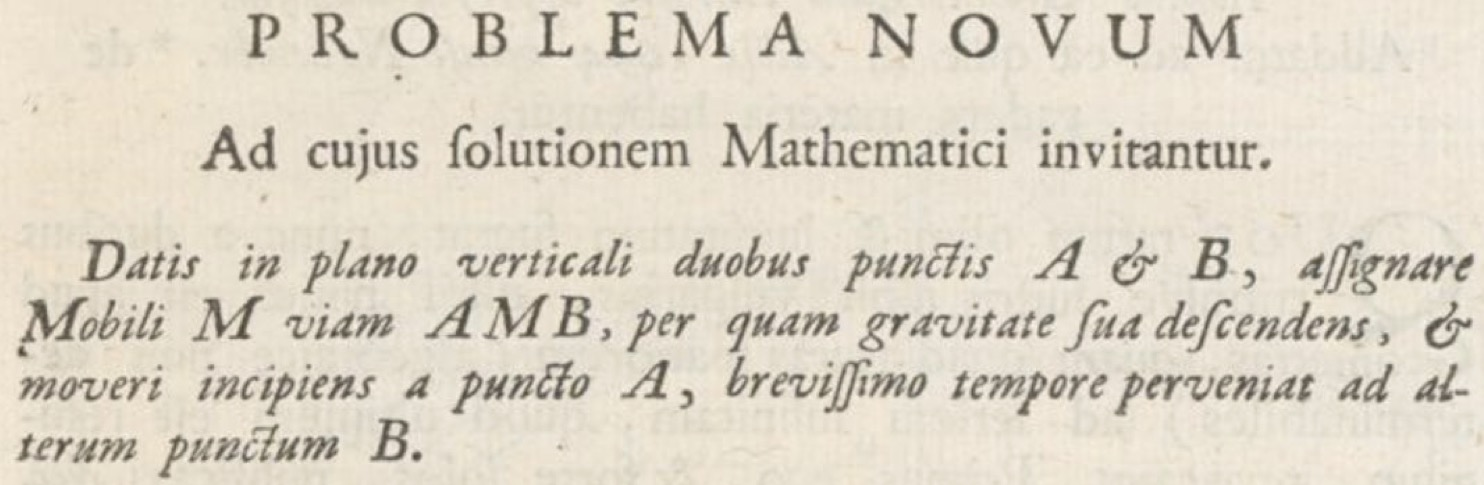
\includegraphics[width=0.8\textwidth]{chapters/020-variation/images/latein.jpg}
\end{center}
Zu deutsch:
\begin{quote}
Neue Aufgabe, zu deren Lösung die Mathematiker eingeladen werden.
Gegeben zwei Punkte $A$ und $B$ in einer vertikalen Ebene, finde
die Bahn $AMB$ eines Punktes $M$, der unter der Wirkung seines
Gewichtes in kürzester Zeit vom Punkt $A$ zum anderen Punkt $B$ absteigt.
\end{quote}
Die Situation der Aufgabenstellung ist in
Abbildung~\ref{buch:variation:fig:brachistochronenproblem}
dargestellt.
Bernoulli hat als Lösung gefunden, dass die Kurve eine Ausschnitt
aus einer Zykloide (in der Abbildung grau) sein muss.
Seine Lösung beruhte auf der Beobachtung, dass sich das Problem analog
zu einem Lichtausbreitungsproblem ist, für welches Fermat bereits
eine Lösung gefunden hat.

Da die Reibung vernachlässigt wird, ist die Energie des Massepunktes
erhalten.
Sie setzt sich aus der potenziellen und der kinetischen Energie
zusammen.
Die potenzielle Energie ist $-mgy$, die kinetische Energie ist
$\frac12mv^2$.
Die Energieerhaltung wird daher zu
\[
E=\frac12mv^2-mgy
\qquad\Rightarrow\qquad
v
=
\sqrt{2g}\!\sqrt{\frac{E}{gm}+y}
=
\!\sqrt{2(C+y)}.
\]
Durch Wahl einer anderen Zeiteinheit kann die Gleichung noch weiter
vereinfacht zu
\(
v = \sqrt{C+y}
\)
vereinfacht werden.
Gesucht ist also die zeitlich kürzeste Bahn eines Teilchens, 
dessen Geschwindigkeit auf bekannte Art $v(y)$ von der vertikalen
Koordinate abhängt.

%
% Das Fermat-Problem
%
\subsection{Das Fermat-Prinzip}
Bereits Fermat hat erkannt, dass das Brechnungsgesetz von Snellius
als Lösung eines Extremalproblems verstanden werden kann.

\begin{satz}[Fermat]
Sie $c/n_i$ die Geschwindigkeit, mit der sich Licht im Medium $M_i$
ausbreitet.
Ein Lichtstrahl von $A_1$ nach $A_2$ geht durch denjenigen Punkt $B$ 
auf der Grenzfläche zwischen den Medien, für den sich die Sinus der
Winkel $\alpha_i$ zwischen den Strahlen und der Normalen zur Grenzfläche
umgekehrt wie die $n_i$ verhalten, wenn also das Brechungsgesetz
\[
\frac{\sin\alpha_1}{\sin\alpha_2}
=
\frac{n_2}{n_1}
\]
gilt.
\end{satz}

\begin{proof}
Ohne der Beschränkung der Allgmeinheit können wir auf die Betrachtung
einer Ebene beschränken, die die beiden Punkte $A_i$ enthält und senkrecht
auf der Grenzfläche steht.
Wir dürfen weiter annehmen, dass die $x$-Achse in der Grenzfläche liegt 
und die Punkte $A_i$ die Koordinaten $(x_i,y_i)$ und der Punkt $B$ die
Koordinaten $(x,0)$ hat.
Es ist derjenige Punkt $x$ zu bestimmen, für den die Lichtzeit entlang 
des Pfades $A_1BA_2$ minimal wird.
Diese Zeit ist
\begin{align*}
t
&=
\frac{\overline{A_1B}}{c/n_1}
+
\frac{\overline{BA_2}}{c/n_2}
\\
ct
&=
n_1\overline{A_1B}
+
n_2\overline{A_2B}
\\
&=
n_1\!\sqrt{(x-x_1)^2 + y_1^2}
+
n_2\!\sqrt{(x_2-x)^2 + y_2^2}
\end{align*}
Das Minimum wird bei einer Nullstelle der Ableitung nach $x$ gefunden,
also bei einer Lösung der Gleichung
\begin{align*}
0
&=
n_1\frac{2(x_1-x)x}{\sqrt{(x_1-x)^2+y_1^2}}
+
n_2\frac{-2(x-x_2)x}{\sqrt{(x_2-x)^2+y_2^2}}.
\intertext{Indem man den zweiten Term auf der rechten Seite auf die linke
Seite bringt und durch $x$ dividiert, erhält man}
n_1
\frac{x_1-x}{\sqrt{(x_1-x)^2+y_1^2}}
&=
n_2
\frac{x-x_2}{\sqrt{(x_2-x)^2+y_2^2}}.
\end{align*}
Der Nenner ist auf beiden Seiten die Hypothenuse eines rechtwinkligen
Dreiecks, welches als Ankathete die Normale zur Grenzfläche hat.
Der Zähler ist die Gegenkathete des Winkels $\alpha_i$ zwischen der
Hypothenuse und der Normalen.
Daher ist der Quotient der Sinus des Winkels oder
\begin{equation}
n_1 \sin\alpha_1 = n_2 \sin\alpha_2.
\label{buch:variation:problem:eqn:snelliusinvariante}
\end{equation}
Die Gleichung~\eqref{buch:variation:problem:eqn:snelliusinvariante}
ist gleichbedeutend mit dem Brechungsgesetz
\[
\frac{\sin\alpha_1}{\sin\alpha_2}
=
\frac{n_2}{n_1}
\]
von Snellius.
\end{proof}

Der Satz von Fermat etabliert das Brechungsgsetz also Lösung eines
Extremalproblems.
Die Natur wählt für einen Lichtstrahl den zeitlich kürzesten Weg.
Der Beweis des Satzes von Fermat zeigt, dass entlang des Lichtstrahls
an jeder Grenzfläche zwischen Medien die Bedingung
\eqref{buch:variation:problem:eqn:snelliusinvariante}
erfüllt.
Wenn die optische Dichte $n$ eine Funktion von $n(y)$ ist, dann
wird der Lichtstrahl nicht nur in diskreten Punkten geknickt, sondern
entlang des ganzen Strahles gekrümmt.
Folgt der Strahl der Kurve $x(y)$, die mit der vertikalen den Winkel
$x'(y) = \tan\alpha(y)$ einschliesst.
Damit lässt sich auch die Sinus-Funktion ausdrücken, es gilt
\[
\sin\alpha(y)
=
\frac{x'(y)}{\pm\!\sqrt{x'(y)^2+1}}.
\]
Aus der Form~\eqref{buch:variation:problem:eqn:snelliusinvariante}
des Brechungsgesetztes wird dann die Gleichung
\begin{equation}
n_1\sin\alpha(y)
=
\frac{n_1(y)x'(y)}{\pm\!\sqrt{x'(y)^2+1}}
=
\operatorname{const}
\qquad\Rightarrow\qquad
\frac{n_1(y)^2x'(y)^2}{x'(y)^2+1}=C.
\label{buch:variation:eqn:fermatdgl}
\end{equation}
Dies ist eine Differentialgleichung für die Funktion $x(y)$.
Sie kann auch in die Form
\[
x'(y)^2
=
\frac{C}{(n_1(y)^2-C)}
\]
gebracht werden.

%
% Das Brachistochronenproblem als Lichtausbreitungsproblem
%
\subsubsection{Das Brachistochronenproblem als Lichtausbreitungsproblem}
Das Fermat-Prinzip besagt, dass ein Lichtstrahl, der sich in einem Medium
mit der Geschwindigkeit $c/n(y)$ ausbreitet, die Gleichung 
\eqref{buch:variation:eqn:fermatdgl} erfüllt.
Beim Brachistochronenproblem ist die Geschwindigkeit $v(y)=\!\sqrt{C-y}$ und 
damit $n(y) = c/\!\sqrt{C-y}$.
Eine Brachistochrone ist also eine Kurve, die die aus
\eqref{buch:variation:eqn:fermatdgl} folgende Gleichung
\begin{equation}
\frac{x'(y)^2}{(1+x'(y)^2)(C-y)} = K
\label{buch:variation:problem:eqn:bernoullidgl}
\end{equation}
erfüllen.

%
% Die Bernoullische Lösung
%
\subsubsection{Die Bernoullische Lösung}
Bernoulli hat gefunden, dass die Brachistochrone ein Zykloidenbogen ist.
Dies lässt sich dadurch verifizieren, dass man die Parametrisierung
einer Zykloide in die
Gleichung~\eqref{buch:variation:problem:eqn:bernoullidgl}
einsetzt.
Die Zykloide hat die Parametrisierung
\[
\left.
\begin{aligned}
x &= r(\varphi - \sin\varphi) 
\\
y &= r(1-\cos\varphi)
\end{aligned}
\right\}
\quad
\text{mit der Ableitung}
\quad
\left\{
\begin{aligned}
\dot{x}(\varphi) &= r(1-\cos\varphi)\\
\dot{y}(\varphi) &= r\sin\varphi
\end{aligned}
\right.
\]
für $\varphi\in\mathbb{R}$.
Die Ableitung ist
\[
x'(y)
=
\frac{\dot{x}(\varphi)}{\dot{y}(\varphi)}
=
\frac{1-\cos\varphi}{\sin\varphi}.
\]
Eingesetzt in \eqref{buch:variation:problem:eqn:bernoullidgl}
wird daraus
\[
\frac{\dot{x}(\varphi)^2}{
(\dot{y}(\varphi)^2 +\dot{x}(\varphi)^2)
(C-r(1-\cos\varphi))
}
=
\frac{(1-\cos\varphi)^2}{
((1-\cos\varphi)^2+\sin^2\varphi)
(C-r+r\cos\varphi)
}
=
K.
\]
Ausmultiplizieren im Nenner ergibt
\[
\frac{(1-\cos\varphi)^2}{
(1-2\cos\varphi+\cos^2\varphi+\sin^2\varphi)
(C-r+r\cos\varphi)
}
=
\frac{1-\cos\varphi}{
2(C-r+r\cos\varphi)
}
\]

%
% Das Brachistochronenproblem als Variationsproblem
%
\subsection{Das Brachistochronenproblem als Variationsproblem
\label{buch:variation:problem:subsection:variationsproblem}}
Die Bernoullische Lösung des Brachistochronenproblems verwendet die
Analogie zum Fermat-Prinzip.
Eine solche Analogie ist nur selten möglich, daher soll das Problem
jetzt in eine Form gebracht werden, in die auch viele ähnliche
Optimierungsproblem gebracht werden können.

Wir erinnern daran, dass die Geschwindigkeit des Massepunktes durch
$v(y)=\sqrt{C-y}$ gegeben ist.
Damit lässt sich die Zeit berechnen, die der Massepunkt entlang der
Lösungskurve braucht, wenn man diese als Funktion $y(x)$ mit beschreibt.
Die Punkte $A$ und $B$ sollen die $x$-Koordinaten $a$ bzw.~$b$ haben.
Für das Kurvenstück zwischen den $x$-Koordinaten $x$ und $x+\Delta x$
braucht der Massepunkt die Zeit
\[
\frac{ \sqrt{\Delta x^2 + \Delta y^2} }{v(y)}
=
\frac{ \sqrt{1 + y'(x)^2} }{ v(y) } \Delta x.
\]
Die Zeit ist das Integral
\begin{equation}
t
=
\int_a^b \frac{\sqrt{1+y'(x)^2}}{v(y(x))}\,dx
=
\int_a^b \sqrt{\frac{1+y'(x)^2}{C-y(x)}}\,dx.
\label{buch:variation:problem:eqn:brachint}
\end{equation}
Der Integrand auf der rechten Seite hängt nur von den Funktion $y(x)$
und $y'(x)$ ab.
Dies kommt vor allem daher, dass die Geschwindigkeit nur von $y$ abhängt,
nicht auch noch von $x$.
Im Allgemeinen wird man also davon ausgehen müssen, dass der Integrand
auch noch von $x$ abhängt.
Die Variationsrechnung befasst sich mit Problemen, in denen Funktionen
gefunden werden müssen, die ein Integral wie das in
\eqref{buch:variation:problem:eqn:brachint}
minimiert oder maximiert werden müssen.

\begin{definition}[Lagrange-Funktion des Brachistochronenproblems]
Die Lagrange-Funk\-tion des Brachistochronenproblems ist der
Integrand des Integrals
\eqref{buch:variation:problem:eqn:brachint},
\index{Lagrange-Funktion}%
also die Funktion
\[
L(x,y,y')
=
\sqrt{\frac{1+y^{\prime 2}}{C-y}}.
\]
\end{definition}

%
% Funktionale
%
\subsection{Funktionale
\label{buch:variation:problem:subsection:funktionale}}
Die Variationsrechnung löst Optimierungsproblem, die von einer
Funktion abhängen.
Um dies mathematisch präzis zu fassen, ist zunächst nötig, die Menge
der in Frage kommenden Funktionen so einzuschränken, dass die interessierende
Grösse überhaupt wohldefiniert ist.

%
% Vektorräume
%
\subsubsection{Vektorräume}
Zunächst sind die gemeinsamen algebraischen Eigenschaften zu charakterisieren,
die wir von den für unsere Untersuchungen zweckmässigen Funktionenmengen
erwarten.

\begin{definition}[Vektorraum]
Ein Vektorraum über den reellen Zahlen $\mathbb{R}$ ist einem Menge $V$ mit
zwei Operationen, der Addition und der Multiplikation mit Skalaren
\begin{align*}
    +\colon V\times V         &\to V : (u,v)\mapsto u+v
&
\cdot\colon \mathbb{R}\times V&\to V : (\lambda,v) \mapsto\lambda v
\end{align*}
mit den folgenden Eigenschaften.
\begin{enumerate}
\item
Es gelten die Assoziativgesetze
\begin{align*}
(u+v)+w&=u+(v+w)&&\text{für alle $u,v,w\in V$}\\
(\lambda \mu)v&=\lambda(\mu v)&&\text{für alle $\lambda,\mu\in\mathbb{R},\;v\in V$.}
\end{align*}
\item
Es gibt einen Vektor $0\in V$ mit der Eigenschaft $0+v=v$ für alle
Vektoren $v\in V$.
\item
Zu jedem Vektor $v\in V$ gibt es den entgegengesetzten Vektor $-v\in V$
mit der Eigenschaft, dass $-v+v=0$ ist.
\item
Die Addition von Vektoren ist kommutativ: $u+v=v+u$ für alle $u,v\in V$.
\item
Es gelten die Distributivgesetze 
\begin{align*}
(\lambda + \mu) v &= \lambda v + \mu v
	&\quad\text{für alle $\lambda,\mu\in\mathbb{R},\;v\in V$}\\
\lambda(u+v)      &= \lambda u + \lambda v
	&\quad\text{für alle $\lambda\in\mathbb{R},\;u,v\in V$}
\end{align*}
\end{enumerate}
\end{definition}

Die Mengen $\mathbb{R}^n$ erfüllen die genannten Eigenschaften, sind
also Vektorräume.
Die Definition eines Vektorraums ist aber viel allgemeiner, insbesondere
gehören dazu auch Mengen von Funktionen.
Damit wird es möglich, die Berechnungen in $\mathbb{R}^n$ auf Funktionen
auszudehnen.
Zum Beispiel bilden die stetigen Funktionen auf einem Intervall einen
Vektorraum, wie das folgende Beispiel zeigt.

\begin{beispiel}
Die Menge
\[
C([a,b])
=
\{f\colon[a,b]\to\mathbb{R}\mid \text{$f$ ist stetig}\}
\]
der stetigen Funktionen bildet einen Vektorraum.
Die Operationen sind die punktweise Addition von Funktionen und die
Multiplikation der Werte mit Skalaren, für $f,g\in C([a,b])$ und
$\lambda\in \mathbb{R}$ ist
\begin{align*}
(f+g)(x) &= f(x)+g(x)
&&\text{und}&
(\lambda f)(x) &= \lambda f(x).
\end{align*}
Entscheidend ist, dass die Addition von Funktionen und die Multiplikation
mit Skalaren nicht aus der Menge herausführt.
Tatsächlich wird in der Analysis gezeigt, dass die Summe stetiger Funktionen
wieder stetig ist und dass die Funktion $x\mapsto \lambda f(x)$ stetig,
wenn $f$ stetig ist.
Die übrigen Eigenschaften sind ebenfalls erfüllt, da sie bereits für die
Funktionswerte erfüllt sind.
\end{beispiel}

%
% Norm und Grenzwerte
%
\subsubsection{Norm und Grenzwerte}
Um Analysis zu betreiben, muss man ausdrücken können, dass eine Folge
von Funktionen konvergiert.
Dazu ist ein Abstandsbegriff zwischen Funktionen nötig.

\begin{definition}[Norm, normierter Raum]
Eine {\em Norm} auf einem Vektorraum $V$ ist eine Abbildung
\index{Norm}%
$\|\cdot\|\colon V\to\mathbb{R}^+_0$ mit nichtnegativen reellen Werten
und den folgenden Eigenschaften
\begin{itemize}
\item Definitheit: $\|v\|\ge 0$ für $v\in V$ mit Gleichheit 
genau dann, wenn $v=0$.
\index{Definitheit}%
\item Absolute Homogenität: Für alle Vektoren $v\in V$ und
\index{Homogenität}%
$\lambda\in\mathbb{R}$ gilt $\|\lambda v\| = |\lambda|\, \|v\|$.
\item Dreiecksungleichung: für alle Vektoren $u,v\in V$ gilt
\index{Dreiecksungleichung}%
$\|u+v\|\le \|u\|+\|v\|$.
\end{itemize}
Ein {\em normierter Raum} ist ein Vektorraum mit einer Norm.
\index{normierter Raum}%
\end{definition}

\begin{beispiel}
Der Vektorraum der stetigen Funktionen kann mit der Supremum-Norm
\[
\|f\| = \sup_{x\in[a,b]} |f(x)|
\]
zu einem normierten Raum gemacht werden.
Die Definitheit ist durch die Definition offensichtlich sichersgtellt.
Für $\|\lambda f\|$ finden wir
\[
\|\lambda f\|
=
\sup_{x\in[a,b]} |\lambda f(x)|
=
|\lambda|\,
\sup_{x\in[a,b]} |f(x)|
=
|\lambda|\, \|f\|,
\]
was die Homogenität zeigt.
Die Dreiecksungleichung folgt aus
\begin{align*}
\|f+g\|
&=
\sup_{x\in[a,b]} |f(x)+g(x)|
\\
&\le
\sup_{x\in[a,b]} (|f(x)|+|g(x)|)
\\
&\le
\sup_{x\in[a,b], y\in[a,b]} (|f(x)|+|g(y)|)
\\
&=
\sup_{x\in[a,b]} |f(x)|
+
\sup_{y\in[a,b]} |g(y)|
=
\|f\| + \|g\|.
\qedhere
\end{align*}
\end{beispiel}

Mit einer Norm ist es jetzt möglich, die Konvergenz von Folgen und den
Begriff des Grenzwertes zu definieren.

\begin{definition}[Cauchy-Folge, Grenzwert]
Eine Folge $(x_n)_{n\in\mathbb{N}}$ in $V$ in einem normierten Raum $V$
mit der Norm $\|\cdot\|$
heisst eine Cauchy-Folge, wenn es für jedes $\varepsilon>0$ eine
\index{Cauchy-Folge}%
$N\in \mathbb{N}$ gibt derart, dass
\[
\| x_n - x_m \| < \varepsilon
\quad\forall n,m\ge N.
\]
Der Vektor $x\in V$ heisst {\em Grenzwert} der Folge $(x_n)_{n\in\mathbb{N}}$,
\index{Grenzwert}%
wenn es zu jedem $\varepsilon > 0$ ein $N\mathbb{N}$ gibt derart, dass
\[
\|x_n-x\| < \varepsilon 
\quad\forall n\ge N.
\]
Die Folge $(x_n)_{n\in\mathbb{N}}$  in $V$ heisst {\em konvergent}, wenn
\index{konvergent}%
$x$ der Grenzwert von $(x_n)_{n\in\mathbb{N}}$ ist.
\end{definition}

Der durch die Supremum-Norm definierte Konvergenzbegriff ist die gleichmässige
Konvergenz.
Zur Erinnerung:
Eine Folge $f_n$ von Funktionen heisst gleichmässig konvergent gegen die
Funktion $f$, wenn es zu jedem
$\varepsilon >0$ ein $N\in\mathbb{N}$ gibt derart, dass
\[
|f_n(x) - f(x)|<\varepsilon\quad\forall n>N\text{ und }x\in [a,b].
\]
Die Supremum-Norm ist
\[
\|f_n(x) - f(x)\|
=
\sup_{x\in[a,b]} |f_n(x)-f(x)| < \varepsilon
\]
für alle $n>N$.
Dies ist genau die Konvergenz in der Norm $\|\cdot\|$.
Aus der Analysis ist bekannt, dass eine gleichmässig konvergente 
Funktionenfolge gegen eine stetige Funktion konvergiert.

\begin{definition}[Banach-Raum]
Ein normierter Raum $V$ heisst ein {\em Banach-Raum},
\index{Banach-Raum}%
wenn jede Cauchy-Folge in $V$ einen Grenzwert hat.
\end{definition}

\begin{beispiel}
Die Menge $C^1([0,2])$
der stetigen Funktionen auf dem Intervall $[0,2]$ ist ein normierter
Raum mit der Norm
\[
\|f\|_1
=
\int_0^2 |f(x)|\,dx,
\]
die auch die $L^1$-Norm heisst.
\index{L1-Norm@$L^1$-Norm}%
Zunächst ist nachzuprüfen, dass dies tatsächlich eine Norm ist.
Die Definitheit und die Homogenität von $\|\cdot\|_1$ ist klar, nur
die Dreiecksungleichung erfordert etwas Arbeit.
Für Funktionen $f,g\in L^1([0,2])$ gilt
\begin{align*}
\|f+g\|_1
&=
\int_0^2 |f(x)+g(x)|\,dx
\\
&\le 
\int_0^2 |f(x)|+|g(x)|\,dx
=
\int_0^2 |f(x)|\,dx
+
\int_0^2 |g(x)|\,dx
=
\|f\|_1+\|g\|_1,
\end{align*}
was die Dreeicksungleichung beweist.

Eine Cauchy-Folge in der $L^1$-Norm muss aber nicht unbedingt einen
stetigen Grenzwert haben.
Die Funktionen
\(
f_n(x) =
\begin{cases}
x^n&\quad x< 1\\
1&\quad x\ge 1
\end{cases}
\)
haben die $L^1$-Norm
\begin{align*}
\|f_n-f_m\|_1
=
\int_0^2 |f_n(x)-f_m|\,dx
\\
&=
\biggl|\int_0^1 x^n-x^m\,dx\biggr|
=
\biggl[
\biggl|
\frac{1}{n+1}x^{n+1}
-
\frac{1}{m+1}x^{m+1}
\biggr|
\biggr]_0^1
\\
&=
\biggl|
\frac{1}{n+1}
-
\frac{1}{m+1}\biggr|.
\end{align*}
Wegen
\[
\|f_n-f_m\|_1
<\varepsilon
\]
für $n,m>2/\varepsilon$ ist $f_n$ eine Cauchy-Folge in $L^1$.
In $L^1$ konvergiert die Folge $f_n$ gegen die Funktion
\[
f(x)
=
\begin{cases}
0&\quad x< 1\\
1&\quad x\ge 1.
\end{cases}
\]
Diese Funktion ist aber nicht stetig, da sie bei $x=1$ einen
Sprung hat.
Bezüglich der $L^1$-Norm ist $C^1([a,b])$ als im Allgemeinen
kein Banach-Raum.
\end{beispiel}

%
% Stetige und differenzierbare Funktionen
%
\subsubsection{Stetige und differenzierbare Funktionen}
Mit der Norm lässt sich auch die Stetigkeit von Abbildungen zwischen
normierten Räumen definieren.

\begin{definition}[Stetigkeit]
Eine Funktion $f\colon U\to V$ zwischen normierten Räumen heisst
{\em stetig im Punkt} $x\in U$, wenn es zu jedem $\varepsilon > 0$
\index{stetig in einem Punkt}%
ein $\delta > 0$
gibt derart, dass
\(
\|f(x)-f(y)\| < \delta
\)
wenn
\(
\|x-y\|<\varepsilon
\).
Eine Funktion $f\colon U\to V$ heisst {\em stetig}, wenn sie in
jedem Punkt von $U$ stetig ist.
\end{definition}

Das Bild einer Folge $x_n\in U$, die gegen $x_0\in U$ konvergiert,
ist eine Folge $f(x_n)$ in $V$.
Man sagt, $y\in V$ sei der Grenzwert von $f(x)$ für $x\to x_0$,
wenn $f(x_n)$ für jede solche Folge $x_n$ gegen $y$ konvergiert.
Der Grenzwert wird auch
\[
\lim_{x\to x_0} f(x)
=
y
\]
geschrieben.
Stetige Funktionen zeichnen sich wie in der Analysis der Funktionen
einer Variablen dadurch aus, dass der Grenzwert der Werte der Funktion
auf einer konvergenten Folge mit dem Funktionswert des Grenzwertes
übereinstimmt.

\begin{satz}
Eine Funktion $f\colon U\to V$ ist genau dann stetig im Punkt $x\in U$,
wenn für jede Folge $x_n$ in $U$ mit Grenzwert $x$ die Folge $f(x_n)$
konvergent ist und
\[
\lim_{n\to\infty} f(x_n) = f(x).
\]
Eine lineare Funktion $f\colon U\to V$ ist genau dann stetig,
wenn für jede Nullfolge $x_n$ in $U$ 
\[
\lim_{n\to \infty} f(x_n) = 0
\]
gilt.
\end{satz}

\begin{definition}
Eine Funktion $f\colon U\to V$ zwischen normierten Räumen heisst
differenzierbar im Punkt $x\in U$ wenn es eine lineare Funktion
$Df(x_0)\colon U\to V$ gibt derart, dass
\[
f(x+v) =f(x) + Df(x_0)\cdot v + o(v),
\]
wobei $o(v)$ bedeutet, dass für diese Funktion
\[
\frac{o(v)}{|v|}\to 0
\quad\text{für $v\to 0$}
\]
gilt.
\end{definition}

Funktionen auf einem Vektorraum mit reellen Werten weren auch
{\em Funktionale} genannt.
\index{Funktional}
Vor dem 20.~Jahrhundert wurde häufig ein Untersschied zwischen
Funktionen von endlich vielen reellen Variablen und Funktionen
von einem unendlichdimensionalen Vektorraum gemacht.
Die Entwicklungen dieses  Abschnittes haben gezeigt, dass eine
solche Unterscheidung nicht gerechtfertigt ist.
Es ist lediglich notwendig, die Definitionen allgemein genug zu
fassen und sich jederzeit über die Funktionenmenge und die zu
verwendende Norm Rechenschaft abzulegen.


%
% 2-fundamtenallemma.tex
%
% (c) 2023 Prof Dr Andreas Müller
%
\section{Das Fundamentallemma
\label{buch:variation:section:fundamentallemma}}
\kopfrechts{Das Fundamentallemma}
Im Fall des endlichdimensionalen Extremalproblems ist aus der
Forderung, dass alle Richtungsableitung verschwinden müssen, 
die Bedingung geworden, dass
\[
v\cdot\grad f = 0
\]
sein muss für alle Vektoren $v\in\mathbb{R}^n$.
Wir haben daraus geschlossen, dass der Gradient $\grad f=0$
sein muss.
Wir hatten dies das endlichdimensionale Fundamentallemma genannt,
wegen $e_k\cdot \grad f = D_kf$ war es eine ziemliche Selbstverständlichkeit.
Bei der Lösung von Variationsproblemen, wo es nicht um endlichdimensionale
Vektoren und das Skalarprodukt, sondern um Funktionen und Integrale
geht, brauchen wir eine ähnliche Aussage für Funktionen.

%
% Positive glatte Funktionen mit kompaktem Träger
%
\subsection{Positive glatte Funktionen mit kompaktem Träger}
Die Aussage des Fundamentallemmas für endlichdimensionale Vektoren 
folgte sofort aus der Tatsache, dass es für jedes $k$ einen Vektor
$e_k$ gibt, der nur in der Koordinaten $k$ von $0$ verschieden ist.
Natürlich gibt es auch Funktionen, die nur in genau einem Punkt
von $0$ verschieden sind.
Eine solche Funktion ist aber im allgemeinen nicht differenzier-
oder integrierbar.
In diesem Abschnitt soll daher gezeigt werden, dass es unendlich
oft stetig differnzierbare Funktionen gibt, die nur in einem beliebig
kleinen vorgegebenen Intervall $\ge 0$ sind.

\begin{definition}[Träger]
Der {\em Träger} einer Funktion $f\colon X\to\mathbb{R}$ ist die Menge
\index{Träger}%
\[
\supp f = \{ x\in X\mid f(x)\ne \}.
\]
\end{definition}

Gesucht ist also eine beliebig oft stetig differenzierbare Funktion,
deren Träger in einem vorgegebenen Intervall $[a,b]$ enthalten ist.
Wir konstruieren so eine Funktion in zwei Schritten.

\input{chapters/020-variation/fig/f.tex}

\begin{satz}
\label{buch:variation:fundamentallemma:satz:glatt}
Die Funktion
\[
f(x)
=
\begin{cases}
e^{-1/x}&\qquad x>0\\
0&\qquad x\le 0
\end{cases}
\]
(siehe auch Abbildung~\ref{buch:variation:fundamentallemma:fig:glatt})
ist beliebig oft stetig differenzierbar.
\end{satz}

\begin{proof}
Es ist klar, dass die Funktion $f$ beliebig oft stetig differenzierbar
ist in jedem Punkt $x\ne 0$.
Es ist also nur nachzuweisen, dass $f(x)$ im Punkt $0$ beliebig
oft stetig differenzierbar ist.

Die ersten drei Ableitungen von $f(x)$ sind
\begin{align}
f'(x) &= \frac{1}{x^2} f(x)
\label{buch:variation:fundamentallemma:eqn:f1}
\\
f''(x) &= \frac{1-2x}{x^4}f(x)
\notag
\\
f'''(x) &= \frac{6x^2-6x+1}{x^6}f(x).
\notag
\end{align}
Daraus lässt sich die Vermutung ableiten, dass
\begin{equation}
f^{(n)}(x)
=
\frac{p_{n-1}(x)}{x^{2n}} f(x)
\label{buch:variation:fundamentallemma:eqn:fabl}
\end{equation}
ist, wobei $p_k(x)$ ein Polynom vom Grad $k$ ist.
Wir beweisen diese Vermutung mit Hilfe von vollständiger Induktion.
Die Induktionsverankerung für die $0$-te Ableitung ist trivial.

Wir nehmen jetzt im Sinne der Induktionsannahme an, dass die $n$-te
Ableitung die Form \eqref{buch:variation:fundamentallemma:eqn:fabl}
hat.
Wir müssen zeigen, dass dann auch $f^{(n+1)}(x)$ diese Form hat.
Dazu berechnen wir
\begin{align}
f^{(n+1)}(x)
&=
\frac{d}{dx}
\frac{p_n(x)}{x^{2n}} f(x)
\notag
\\
&=
\frac{p_n'(x)}{x^{2n}} f(x)
-2n
\frac{p_n(x)}{x^{2n+1}} f(x)
+
\frac{p_n(x)}{x^{2n}} f'(x).
\notag
\intertext{Mit der ersten Ableitung
\eqref{buch:variation:fundamentallemma:eqn:f1} wird dies zu}
&=
\frac{p_n'(x)}{x^{2n}} f(x)
-2n
\frac{p_n(x)}{x^{2n+1}} f(x)
+
\frac{p_n(x)}{x^{2n}} \frac{1}{x^2}f(x)
\notag
\\
&=
\frac{x^2p_n'(x) -2nxp_n(x)+p_n(x)}{x^{2n+2}} f(x).
\label{buch:variation:fundamentallemma:eqn:induktionsschritt}
\end{align}
Die Ableitung $p_n'(x)$ ist ein Polynom vom Grad $n-1$ und damit
ist $x^2p_n'(x)$ ein Polynom vom Grad $n+1$.
Ebenso ist $xp_n(x)$ ein Polynom vom Grad $n+1$ während
$p_n(x)$ ein Polynom vom Grad $n$ ist.
Der Zähler von
\eqref{buch:variation:fundamentallemma:eqn:induktionsschritt}
ist
\[
p_{n+1}(x)
=
x^2p_n'(x)+(1 -2nx)p_n(x),
\]
ein Polynom vom Grad $n+1$.
Damit ist der Induktionsschritt erfolgreich und die Behauptung betreffend
die Form von $f^{(n)}(x)$ ist bewiesen.

Es ist jetzt nur noch zu zeigen, dass der Grenzwert von $f^{(n)}(x)$
für $x\to 0+$ verschwindet.
Da das Polynom $p_n(x)$ stetig ist, folgt
\[
\lim_{x\to 0}
f^{(n)}(x)
=
\lim_{x\to 0}\frac{p_n(x)}{x^{2n}}f(x)
=
p_n(0) \lim_{t\to\infty} t^{2n} e^{-t}
=
0.
\]
Damit ist die beliebige stetige Differenzierbarkeit an der Stelle
$x=0$ gezeigt.
\end{proof}

Die Funktion $f(x)$ von 
Satz~\ref{buch:variation:fundamentallemma:satz:glatt} 
erfüllt noch nicht die Forderung, dass sie nur in einem vorgegebenen
Intervall von $0$ verschieden ist.

\input{chapters/020-variation/fig/g.tex}

\begin{satz}
\label{buch:variation:fundamentallemma:satz:gab}
Sei $f(x)$ die Funktion von
Satz~\ref{buch:variation:fundamentallemma:satz:glatt}.
Dann ist
\[
g_{a,b}(x)
=
f(x-a) f(b-x)
\]
eine unendlich oft stetig differenzierbare, nichtnegative Funktion mit Träger
$\supp g_{a,b}=(a,b)$.
\end{satz}

Die Funktionen $g_{a,b}(x)$ sind beliebig oft differenzierbar und nur im
Intervall $[a,b]$ von $0$ verschieden und sogar positiv.
Weil sie stetig sind, sind sie auch integrierbar, man kann also das
Integral über $\mathbb{R}$ berechnen und die Funktion damit normieren.
Die neue Funktion
\[
\frac{1}{N}
\tilde{g}_{a,b}(x)
\qquad\text{mit}\;
N
=
\int_{-\infty}^{\infty}g_{a,b}(x)\,dx
=
\int_a^b g_{a,b}(x)\,dx
\]
ist immer noch beliebig oft stetig differenzierbar und hat zusätzlich die
Eigenschaft
\[
\int_{-\infty}^{\infty}
\tilde{g}_{a,b}(x)\,dx
=
\int_a^b
\tilde{g}_{a,b}(x)\,dx
=
1.
\]
Wir formulieren dieses Resultat als Satz.

\begin{satz}
\label{buch:variation:satz:gabeins}
Zu jedem Intervall $[a,b]$ gibt es eine beliebig oft stetig
differenzierbare Funktion $g(x)$, genau das Intervall $[a,b]$
als Träger hat und deren Integral über $[a,b]$ den Wert $1$ hat.
\end{satz}

%
% Das Fundamentallemma
%
\subsection{Das Fundamentallemma}
Mit der Funktion $g_{a,b}(x)$ von
Satz~\ref{buch:variation:fundamentallemma:satz:gab}
lässt sich jetzt das Fundamentallemma in der folgenden Form
leicht beweisen.

\begin{satz}[Fundamentallemma]
\label{buch:variation:fundamentallemma:satz:fundamentallemma}
Wenn für die stetige Funktion $f\colon[a,b]\to\mathbb{R}$ 
\begin{equation}
\int_a^b f(x)\varphi(x)\,dx = 0
\label{buch:variation:fundamentallemma:eqn:fundamentalbed}
\end{equation}
gilt für jede beliebig oft stetig differenzierbare Funktion $\varphi(x)$ 
dann ist $f(x)=0$.
Das Resultat gilt selbst dann, wenn
\eqref{buch:variation:fundamentallemma:eqn:fundamentalbed}
nur für beliebig oft stetig differenzierbare Funktionen $\varphi(x)$ 
gilt, die ausserdem an den Intervallenden verschwinden:
$\varphi(a)=\varphi(b)=0$.
\end{satz}

\begin{proof}
Wir zeigen mit Hilfe eines Widerspruchs, dass es keinen Punkt $x_0\in[a,b]$
geben kann, für den $f(x_0)\ne 0$ ist.
Dazu nehmen wir also an, dass $f(x_0)\ne 0$ ist.
Falls $f(x_0)<0$ ist, ersetzen wir $f$ durch $-f$, 
die Bedingung
\eqref{buch:variation:fundamentallemma:eqn:fundamentalbed}
ändert sich dadurch nicht.
\input{chapters/020-variation/fig/fundamentallemma.tex}
Wir dürfen daher annehmen, dass $f(x_0)>0$ ist
(Abbildung~\ref{buch:variation:fundamentallemma:fig:beweis}).
Da $f$ stetig ist, gibt es ein Intervall $[x_0-\varepsilon,x_0+\varepsilon]$
derart, dass $f(x)> \frac12 f(x_0)$ für
$x\in[x_0-\varepsilon,x_0+\varepsilon]$ gilt.
Dann gilt für das Integral
\[
\int_a^b
f(x)
g_{x_0-\varepsilon,x_0+\varepsilon} (x)
\,dx
>
\frac{f(x_0)}{2}
\int_a^b
g_{x_0-\varepsilon,x_0+\varepsilon} (x)
\,dx
>
0
\]
im Widerspruch zur Bedingung
\eqref{buch:variation:fundamentallemma:eqn:fundamentalbed}.
Der Widerspruch zeigt, dass $f(x)=0$ sein muss.
\end{proof}

%
% Skalarproduktformulierung des Fundamentallemmas
%
\subsection{Skalaproduktformulierung des Fundamentallemmas}
Die Richtungsableitung einer Funktion endlich vieler Variablen 
konnte als Skalarprodukt mit dem Gradienten geschrieben werden und
das Fundamentallemma hat besagt, dass der Gradient verschwindet,
wenn alle Richtungsableitungen verschwinden.
Diese Schlussweise ist auch für Funktionen möglich, wenn man Funktionen
ein Skalarprodukt definieren kann.

\begin{definition}[$L^2$-Skalarprodukt]
Das {\em Skalarprodukt} zweier quadratintegrierbarer Funktion $f$ und $g$
auf dem Intervall $[a,b]$ ist definiert durch
\[
\langle f,g\rangle
=
\int_a^b f(x)g(x)\,dx.
\]
\end{definition}

\begin{satz}[Fundamentallemma, Skalarproduktform]
Wenn für eine stetige Funktion $f\colon[a,b]\to\mathbb{R}$ das Skalarprodukt
\[
\langle f,\varphi\rangle = 0
\]
ist für jede unendlich oft differenzierbare Funktion $\varphi$ auf dem
Intervall $[a,b]$, dann ist $f=0$.
\end{satz}



%
% 3-eulerlagrange.tex
%
% (c) 2023 Prof Dr Andreas Müller
%
\section{Die Euler-Lagrange Differentialgleichung
\label{buch:variation:section:eulerlagrange}}
\kopfrechts{Die Euler-Lagrange Differentialgleichung}
Das Neuartige an der Aufgabenstellung des Brachistochronenproblems
war, dass eine Funktion gesucht war, so dass ein damit gebildetes
Integral eine Minimaleigenschaft erfüllt.
Für die damalige Mathematik war die Aufgabe, eine Funktion zu finden,
nicht neu.
Die Theorie der Differentialgleichungen war bereits entwickelt,
Newton hat die Infinitesimalrechnung ja erfunden, um damit die
Bewegungsgleichungen der Physik zu formulieren und zu lösen.
In einer Differentialgleichung werden Werte und Ableitungen einer
Funktion an einer einzigen Stelle miteinander verbunden.
Etwas salop formuliert sagt die Differentialgleichung in jedem
Punkt, in welche Richtung und mit welcher Krümmung die Funktionskurve
weiter zu zeichnen ist.

Im Brachistochronenproblem tragen aber alle Werte der gesuchten
Funktion zum Integral bei, es scheint daher auf den ersten Blick
nicht möglich, das Problem durch schrittweise Konstruktion
``von Punkt zu Punkt'' der Lösungskurve zu konstruieren.

Bernoullis Lösung des Brachistochrononproblems beruht auf der
Beobachtung, dass sich die Bedinung für die schnellste Bahn
durch eine Bedingung ersetzen lässt, die in jedem einzelnen
Punkt ausgewertet werden kann.
Das von ihm verwendete Fermat-Prinzip wurde ursprünglich ebenfalls
als eine globale Eigenschaft eines Lichtstrahls formuliert.
Aus dem Fermat-Prinzip folgt aber das Brechungsgesetz, welches
sagt, dass die Richtung eines Strahls in einem Punkt genau dann
ändert, wenn sich dort auch der Brechungsindex der beiden Medien
ändert.
Das Fermat-Prinzip ist also ein Beispiel dafür, wie eine globale
Bedingung erfüllt werden kann, indem einer lokalen Regel in jedem
Punkt gefolgt wird.

Es ist das Verdienst von Euler und Lagrange, zu erkennen, dass diese
Übersetzung eines globalen Variationsproblems in ein lokales 
Problem immer möglich ist.
Es entsteht dabei die Euler-Lagrange-Differentialgleichung, welche
die Problemstellung auf die Lösung einer Differentialgleichung
reduziert.
Damit ist ein allgemein anwendbares Lösungsverfahren gefunden.
Zu einem Variationsproblem lässt sich immer eine Differentialgleichung
finden, welche die gesuchte Funktion als Lösung hat.

In diesem Abschnitt soll dieser indirekte Weg der Lösung von
Variationsaufgaben dargestellt werden.
Wir werden später zeigen, dass diese Vorgehensweise nicht immer
erfolgreich sein kann.
Zum Beispiel werden wir in Kapitel~\ref{buch:chapter:nichtdiff}
Variationsprobleme kennenlernen, deren Lösungskurven nicht
differenzierbar sind und daher auch nicht von einer Differentialgleichung
gefunden werden können.
Im Kapitel~\ref{buch:chapter:direkt} werden daher die sogenannten
direkten Methodn vorgestellt, die den Umweg über eine
Differentialgleichung vermeiden.

%
% Die Lagrange-Funktion
%
\subsection{Die Lagrange-Funktion
\label{buch:variation:eulerlagrange:subsection:lagrange-funktion}}
Wir betrachten Variationsproblem der folgenden Art.
Gesucht ist eine auf dem Intervall $[x_0,x_1]$ definirte
Funktion $y(x)$, die das Integral
\begin{equation}
I(y)
=
\int_{x_0}^{x_1}
F(x, y(x), y'(x))
\,dx
\label{buch:variation:eulerlagrange:eqn:funktional}
\end{equation}
maximiert oder minimiert.
Der Ausdruck~\eqref{buch:variation:eulerlagrange:eqn:funktional}
wird ein Funktional genannt.
Die Funktion
\[
F
\colon
\mathbb{R}\times
\mathbb{R}\times
\mathbb{R}
\to
\mathbb{R}
\]
von drei Variablen heisst die {\em Lagrange-Funktion}
des Funktionals \eqref{buch:variation:eulerlagrange:eqn:funktional}.

\begin{beispiel}
Die Lagrange-Funktion des Brachistochronenproblems ist
\[
F(x,y,y')
=
\sqrt{ \frac{1+y^{\prime 2}}{y} }.
\]
Die Funktion hängt nicht von $x$ ab, was bedeutet, dass eine
Verschiebung in $x$-Richtung die Form der Lösungsfunktion des
Variationsproblems nicht ändert.
\end{beispiel}

\begin{beispiel}
\label{buch:variation:eulerlagrange:beispiel:gerade}
Wir formulieren die Aufgabe, die kürzeste Verbindung der Punkte
$(x_0,y_0)$ und $(x_1,y_1)$ in einer Ebene zu finden, als Variationsproblem.
Die Länge einer Kurve $y(x)$ ist das Integral
\[
l(y)
=
\int_{x_0}^{x_1}
\sqrt{1+y'(x)^2}\,dx.
\]
Daraus lesen wir ab, dass die Lagrange-Funktion dieses Variationsproblems
\begin{equation}
F(x,y,y') = \sqrt{1+y^{\prime 2}}
\label{buch:variation:eulerlagrange:eqn:geradeL}
\end{equation}
ist.
Die Funktion hängt weder von $x$ noch von $y$ ab.
Dies ist auch zu erwarten, denn die Länge einer Kurve hängt nicht davon
ob, wo in der Ebene sie platziert ist.
Eine Verschiebung in $x$-Richtung würde das $x$-Argument ändern,
eine Verschiebung in $y$-Richtung die $y$-Werte.
Wäre $F$ von $x$ oder $y$ abhängig, könnte auch die Länge der Kurve
davon abhängen.
\end{beispiel}

%
% Euler-Lagrange_Differentialgleichung
%
\subsection{Euler-Lagrange-Differentialgleichung
\label{buch:variation:eulerlagrange:subsection:dgl}}
\input{chapters/020-variation/fig/variation0.tex}
Das Maximum oder Minimum einer Funktionen mehrere Variablen wurde
gefunden, indem die Richtungsableitung berechnet und $=0$ gesetzt
wurde.
Um die Funktion zu bestimmen, die ein Funktional $I(y)$ zu einem
Maximum oder Minimum macht, versuchen wir, die Idee der Richtungsableitung
für ein Funktional nachzuahmen.
Wir nehmen daher an, dass $y(x)$ eine Funktion ist, die das Funktional
$I(y)$ zu einem Minimum macht.
Für die Richtungsableitung addieren wir ein Vielfaches einer
Funktion $\eta(x)$, die Summe $y(x)+\varepsilon\eta(x)$ entspricht
dann einer Geraden mit Richtung $\eta(x)$ im Funktionenraum
(Abbildung~\ref{buch:variation:fig:variation0}).
Die Funktionen $y(x)+\varepsilon\eta(x)$ sind aber nur dann Kandidaten
für eine Lösung des Problems, wenn immer noch
\begin{align*}
y(x_0) + \varepsilon \eta(x_0) &= y_0
&&\text{und}&
y(x_1) + \varepsilon \eta(x_1) &= y_1
\end{align*}
gilt.
Dies ist nur möglich, wenn $\eta(x_0)=\eta(x_1)=0$ ist.

Wir berechnen jetzt die Ableitung der Funktion
$\varepsilon\mapsto I(y+\varepsilon\eta )$ an der Stelle $\varepsilon=0$.
Da die Intervallgrenzen nicht von $\varepsilon$ abhängen, können wir
die Ableitung unter das Integral nehmen:
\begin{align*}
\frac{d}{d\varepsilon}
I(y+\varepsilon\eta)
&=
\int_{x_0}^{x_1}
\frac{d}{d\varepsilon}
F(x,y(x)+\varepsilon\eta(x),y(x)+\varepsilon\eta'(x))
\,dx.
\intertext{Da $F$ differenzierbar ist, kann die Ableitung mit der
Kettenregel berechnet werden, sie ist}
&=
\int_{x_0}^{x_1}
\frac{\partial F}{\partial y}
(x,y(x)+\varepsilon\eta(x),y(x)+\varepsilon\eta'(x))
\eta(x)
\\
&\qquad
+
\frac{\partial F}{\partial y'}
(x,y(x)+\varepsilon\eta(x),y(x)+\varepsilon\eta'(x))
\eta'(x)
\,dx.
\intertext{Uns interessiert aber nur der Wert an der Stelle $\varepsilon=0$,
er ist}
\frac{d}{d\varepsilon}
I(y+\varepsilon\eta)
\bigg|_{\varepsilon=0}
&=
\int_{x_0}^{x_1}
\frac{\partial F}{\partial y}
(x,y(x),y'(x))
\,
\eta(x)
+
\frac{\partial F}{\partial y'}
(x,y(x),y'(x))
\,
\eta'(x)
\,dx
=0.
\end{align*}
Das Integral hängt von den verschiedenen Faktoren $\eta(x)$ und
von $\eta'(x)$ in den beiden Termen unter dem Integral ab.
Wir integrieren den zweiten Term partiell 
\begin{align*}
\int_{x_0}^{x_1}
\frac{\partial F}{\partial y'}(x,y(x),y'(x))\,\eta'(x)\,dx
&=
\biggl[
\frac{\partial F}{\partial y'}(x,y(x),y'(x))\,\eta(x)
\biggr]_{x_0}^{x_1}
\\
&\qquad
-
\int_{x_0}^{x_1}
\frac{d}{dx}
\frac{\partial F}{\partial y'}(x,y(x),y'(x))\,\eta(x)\,dx.
\end{align*}
Da $\eta(x_0)=\eta(x_1)=0$ verschwindet der erste Term
auf der rechten Seite, es bleibt
\[
\frac{d}{d\varepsilon}
I(y+\varepsilon\eta)
\bigg|_{\varepsilon=0}
=
\int_{x_0}^{x_1}
\biggl(
\frac{\partial F}{\partial y}
(x,y(x),y'(x))
-
\frac{d}{dx}
\frac{\partial F}{\partial y'}
(x,y(x),y'(x))
\biggr)
\eta(x)
\,dx.
\]
Dies kann auch als Skalarprodukt
\[
\biggl\langle 
\frac{\partial F}{\partial y}
(x,y(x),y'(x))
-
\frac{d}{dx}
\frac{\partial F}{\partial y'}
(x,y(x),y'(x))
,
\eta(x)
\biggr\rangle
=
0
\]
geschrieben werden.
Da dies für jede differenzierbare Funktion $\eta$ mit Randwerten
$\eta(x_0)=\eta(x_1)$ gelten muss, folgt nach dem
Fundamentallemma~\ref{buch:variation:fundamentallemma:satz:fundamentallemma},
der folgende Satz. 

\begin{satz}[Euler-Lagrange]
\label{buch:variation:eulerlagrange:satz:eulerlagrange}
Wenn die mindestens zweimal stetig differenzierbare Funktion $y(x)$
unter allen solchen Funktionen mit $y(x_0)=y_0$ und $y(x_1)=y_1$
das Funktional
\[
I(y)
=
\int_{x_0}^{x_1}
F(x,y(x),y'(x))\,dx
\]
zu einem Maximum oder Minimum macht, dann ist $y(x)$ eine Lösung der
gewöhnlichen Differentialgleichung
\begin{equation}
\frac{d}{dx}
\frac{\partial F}{\partial y'}(x,y(x),y'(x))
-
\frac{\partial F}{\partial y}(x,y(x),y'(x))
=
0.
\label{buch:variation:eulerlagrange:eqn:eulerlagrange}
\end{equation}
Sie heisst die {\em Euler-Lagrange-Differentialgleichung}.
\end{satz}

Eine Lösung des Variationsproblems kann also als Lösung der
Euler-Lagrange-Dif\-fe\-ren\-tial\-glei\-chung mit den Randwerten
$y(x_0)=x_0$ und $y(x_1)=y_1$ gefunden werden.
Die Bedingung ist notwendig, aber nicht hinreichend.
Wie bei der Bestimmung eines Extremums bei Funktionen endlich
vieler Variablen garantiert das Verschwinden der Richtungsableitung
nicht, dass auch tatsächlich ein Extremum vorliegt.
Man sagt daher auch, dass eine Lösung $y(x)$ der
Euler-Lagrange-Differentialgleichung das Funktional $I(y)$
stationär macht.

Eine weitere Einschränkung ist, dass die Herleitung der
Euler-Lagrange-Differential\-gleichung vorausgesetzt hat,
dass die Lösungsfunktion $y(x)$ mindestens zweimal 
stetig differenzierbar ist.
Es gibt aber durchaus Variationsprobleme, deren Lösungen
nicht differenzierbar sind, dazu mehr im Kapitel~\ref{buch:chapter:nichtdiff}.

\begin{beispiel}
\label{buch:variation:eulerlagrange:beispiel:gerade}
Wir lösen das Variationsproblem von Beispiel
\ref{buch:variation:eulerlagrange:beispiel:gerade}
mit der Lagrange-Funk\-tion
\eqref{buch:variation:eulerlagrange:eqn:geradeL}.
Da die Lagrange-Funktion nicht von $y$ abhängt, bleibt von der 
Euler-Lagrange-Gleichung nur
\[
\frac{d}{dx}
\frac{\partial L}{\partial y'}(x,y(x),y'(x))
=
0
\]
übrig.
Berechnung der Ableitung liefert
\begin{equation}
\frac{\partial}{\partial y'}
\sqrt{1+y^{\prime 2}}
=
\frac{y'}{\sqrt{1+y^{\prime 2}}}.
\label{buch:variation:eulerlagrange:eqn:ableitungFyp}
\end{equation}
Die Ableitung nach $x$ ergibt
\begin{align*}
\frac{d}{dx}
\frac{\partial}{\partial y'}
\sqrt{1+y^{\prime 2}}
&=
\frac{d}{dx}
\frac{y'}{\sqrt{1+y^{\prime 2}}}
\\
&=
\frac{
y''\sqrt{1+y^{\prime 2}}-y'\cdot \frac{y'y''}{\sqrt{1+y^{\prime 2}}}
}{
1+y^{\prime 2}
}
\\
&=
y''
\frac{
1+y^{\prime 2}-y^{\prime 2}
}{
(1+y^{\prime 2})^{\frac32}
}.
\intertext{Die Euler-Lagrange-Differentialgleichung ist daher}
0
&=
\frac{y''}{(1+y^{\prime 2})^{\frac32}} .
\end{align*}
Der Nenner auf der rechten Seite ist immer $\ge 1$, die Gleichung kann
also nur erfüllt sein, wenn $y''=0$ ist.
Die Funktion $y(x)$ muss also eine lineare Funktion $y=ax+b$ sein.
Die Randbedingung wird erfüllt für die Geradengleichung
\[
y(x)
=
\frac{y_1-y_0}{x_1-x_0}(x-x_0) + y_0.
\]
Kürzeste Verbindungen in der Ebene sind daher Geraden.
\end{beispiel}

%
% Freie Randbedingungen
%
\subsection{Freie Randbedingungen
\label{buch:variation:eulerlagrange:subsection:freierb}}
In der Herleitung der Euler-Lagrange-Differentialgleichung wurde angenommen,
dass die Endpunkte der Lösungsfunktion durch $y(x_0)=y_0$ und $y(x_1)=y_1$
fest vorgegeben sind.
Diese Voraussetzung soll in diesem Abschnitt abgeschwächt werden.
Die Funktionswerte in den Endpunkten sollen also nicht mehr fest
vorgegeben sein.

\begin{beispiel}
\label{buch:variation:eulerlagrange:beispiel:freiegerade}
Im Beispiel~\ref{buch:variation:eulerlagrange:beispiel:gerade}
wurde die kürzeste Kurve zwischen zwei Punkten in der Ebene
gesucht und wie erwartet eine Gerade als Lösung gefunden.
Wenn die Werte $y_0$ und $y_1$ jetzt nicht mehr vorgegeben sind,
wird die kürzeste Verbindung zwischen den beiden Geraden
$x=x_0$ und $x=x_1$ gesucht.
Die Lösung dieses Problems ist nicht eindeutig, jede horizontale
Strecke mit $y_0=y_1$ ist eine Lösung.
\end{beispiel}

Das Beispiel zeigt, dass es im Allgemeinen immer noch die Vorgabe
eines der beiden Randwerte braucht, um die Lösung eindeutig zu
bestimmen.
Wir lösen daher die folgende Aufgabe.

\begin{aufgabe}
Gesucht ist eine zweimal stetig differnzierbare Funktion $y(x)$ auf
dem Intervall $[x_0,x_1]$ mit $y(x_0)=y_0$, die das Integral
\[
I(y)
=
\int_{x_0}^{x_1} F(x,y(x),y'(x))\,dx
\]
zu einem Extremum macht.
Am rechten Ende des Intervalls ist der Funktion $y(x)$ keine
Randbedingung auferlegt.
\end{aufgabe}

\begin{proof}[Lösung]
\input{chapters/020-variation/fig/variation1.tex}
Sei $y(x)$ eine Lösung der Aufgabe und sei $y_1:=y(x_1)$ der Wert
der Lösung am rechten Rand des Intervalls.
Wir berechnen wieder die Variation von $I(y)$ mit Hilfe von
stetig differenzierbaren Funktionen $\eta(x)$, die jetzt aber 
nur noch die Bedingungn $\eta(x_0)=0$ erfüllen müssen
(Abbildung~\ref{buch:variation:fig:variation1}).
Die Richtungsableitung ist wie früher
\begin{align*}
\frac{d}{d\varepsilon}
I(y+\varepsilon\eta)
\bigg|_{\varepsilon=0}
&=
\frac{d}{d\varepsilon}
\int_{x_0}^{x_1}
F(x,y(x)+\varepsilon\eta(x),y'(x)+\varepsilon\eta'(x))\,dx
\\
&=
\int_{x_0}^{x_1}
\frac{\partial F}{\partial y}(x,y(x),y'(x)) 
\eta(x)
+
\frac{\partial F}{\partial y'}
(x,y(x),y'(x))
\eta'(x)
\,dx
\intertext{und mit partieller Integration}
&=
\biggl[
\frac{\partial F}{\partial y'}(x,y(x),y'(x)) \eta(x)
\biggr]_{x_0}^{x_1}
\\
&\qquad
+
\int_{x_0}^{x_1}
\biggl(
\frac{\partial F}{\partial y}(x,y(x),y'(x))
-
\frac{d}{dx}
\frac{\partial F}{\partial y'}(x,y(x),y'(x))
\biggr)
\,
\eta(x)
\,dx.
\end{align*}
Im Gegensatz zu früher können wir jetzt aber nicht mehr
schliessen, dass der erste Term verschwindet, da $y(x_1)$ nicht
mehr als $=0$ verausgesetzt wird.
Vielmehr erhalten wir für die erste Variation
\begin{equation*}
\delta I(y)
=
\frac{\partial F}{\partial y'} (x_1,y(x_1),y'(x_1)) \eta(x_1)+
\int_{x_0}^{x_1}
\biggl(
\frac{\partial F}{\partial y}(x,y(x),y'(x))
-
\frac{d}{dx}
\frac{\partial F}{\partial y'}(x,y(x),y'(x))
\biggr)
\,
\eta(x)
\,dx.
\end{equation*}
Die Klammer im Integral ist von der Euler-Lagrange-Differentialgleichung
her bekannt, aber es ist ein weiterer hinzugekommen, der genau dann
verschwindet wenn auch $\eta(x_1)=0$ ist.

Dann ist $y(x)$ natürlich erst recht eine Lösung des Problems, das
Funktional $I(y)$ mit den {\em zwei} Randbedingungen
$y(x_0)=y_0$ und $y(x_1)=y_1$ zu einem Extremum zu machen, also
muss die Funktion $y(x)$ sicher die Euler-Lagrange-Differentialgleichung
erfüllen.
Die Klammer im Integral wird daher verschwinden, die Variation
reduziert sich auf den ersten Term
\[
\delta I(y)
=
\frac{\partial F}{\partial y'} (x_1,y(x_1),y'(x_1)) \eta(x_1)
=
0.
\]
Sie verschwindet nur dann für alle zulässigen Funktionen $\eta(x)$, wenn
\begin{equation*}
\frac{\partial F}{\partial y'}(x_1,y(x_1),y'(x_1))=0
\end{equation*}
gilt.
Dies ist eine zusätzliche Randbedingung für die Funktion $y(x)$, geschrieben
in einer impliziten Form.
\end{proof}

Wir halten das Resultat der Aufgabenlösung als Satz fest:

\begin{satz}
\label{buch:variation:eulerlagrange:satz:zusaetzlicherb}
Wenn die zweimal stetig differenzierbare Funktion $y(x)$ mit dem
Randwert $y(x_0)=y_0$ das Integral
\[
I(y)
=
\int_{x_0}^{x_1} F(x,y(x),y'(x))\,dx
\]
zu einem Extremum macht, dann erfüllt sie am rechten Intervallende
die Randbedingung
\begin{equation}
\frac{\partial F}{\partial y'}(x_1,y(x_1),y'(x_1))=0.
\label{buch:variation:eulerlagrange:eqn:zusaetzlicherb}
\end{equation}
zusätzlich zur Euler-Lagrange-Gleichung für die Lagrange-Funktion $F$.
\end{satz}

\begin{beispiel}
\label{buch:variation:eulerlagrange:beispiel:einseitigegerade}
Wir betrachten wieder das Funktional
\[
I(y)
=
\int_{x_0}^{x_1}
\sqrt{1+y^{\prime 2}(x)}
\,dx
\]
mit der einzigen Randbedingung $y(x_0)=y_0$, der Funktionswert auf 
der rechten Seite ist nicht vorgebeben.
Der Satz~\eqref{buch:variation:eulerlagrange:satz:zusaetzlicherb}
besagt zunächst, dass die Lösungsfunktion wieder eine Gerade sein
muss, da die Euler-Lagrange-Gleichung erfüllt sein muss.
Zusätzlich muss aber auch die Randbedingung
\eqref{buch:variation:eulerlagrange:eqn:zusaetzlicherb}
am rechten Ende des Intervalls erfüllt sein.
Die Ableitung der Lagrange-Funktion ist in diesem Fall durch
\eqref{buch:variation:eulerlagrange:eqn:ableitungFyp}
gegeben, es muss also
\[
\frac{y'(x_1)}{\sqrt{1+y'(x_1)^2}}
=
0
\qquad\Rightarrow\qquad y'(x_1)=0
\]
gelten.
Die Lösung ist daher wie erwartet eine horizontale Strecke.
\end{beispiel}



%
% 5-hoehereableitungen.tex
%
% (c) 2023 Prof Dr Andreas Müller
%
\section{Höhere Ableitungen
\label{buch:variation:section:hoehereableitungen}}
\kopfrechts{Höhere Ableitungen}
Das Beispiel der Spline-Interpolation in
Abschnitt~\ref{buch:nichtdiff:section:splines}
zeigt, dass es manchmal
nötig ist, höhere Ableitungen als die erste in einem Funktional
zu berücksichtigen.
In diesem Abschnitt wird die Theorie der ersten Variation auf
Funktionale erweitert, die von beliebigen Ableitungen der Funktion $y(x)$
abhängen.

%
% Lagrange-Funktion mit höheren Ableitungen
%
\subsection{Lagrange-Funktion mit höheren Ableitungen}
Die Euler-Lagrange-Differentialgleichung wurde bisher für Funktionale
hergeleitet, deren Lagrange-Funktion von $x$, der Funktion $y(x)$ und
der ersten Ableitung $y'(x)$ abhängen.

\begin{definition}
Eine Funktion $L(x,y,y',\dots,y^{(n)})$ heisst eine Lagrange-Funktion
der Ordnung $n$.
\index{Lagrange-Funktion $n$-ter Ordnung}%
\end{definition}

\begin{beispiel}
Das Variationsproblem für die Spline-Integration hat die Lagrange-Funktion
zweiter Ordnung
\[
L(x,y,y',y'') = y^{\prime\prime 2}
\]
verwendet.
\end{beispiel}

Ein elastischer Stab speichert bei Verbiegung Energie, deren Dichte
entlang des Stabes proportional zur Krümmung ist.
Ist $s\mapsto \gamma(s)\in\mathbb{R}^2$ eine differenzierbare
Parametrisierung einer ebenen Kurve, die die Form eines dünnen elastischen
Stabes beschreibt, dann ist die Gesamtenergie des Stabes bis auf
eine Konstante durch das Integral
\[
E
=
\int_a^b \kappa(s)^2 \,ds
\]
gegeben
Ist $s$ ein Bogenlängenparameter, also $|\dot{\gamma}(s)|=1$, dann ist
die Krümmung die zweite Ableitung, also
\[
I = \int_a^b \ddot{\gamma}(s)^2\,ds.
\]
Diese Parameterdarstellung ist aber nicht die Form, in der wir bis jetzt
Kurven in der Ebene beschreiben konnten.

Sei $y(x)$ eine Funktion, deren Graph einen elastisch verbogenen Stab
in der Ebene beschreibt.
Die Krümmung des Graphen kann nach
\[
\kappa(x)
=
\frac{y''(x)}{(1+y'(x)^2)^{\frac32}}
\]
berechnet werden.
Die Energie des Stabes wird dann
\[
E
=
\int_a^b \frac{y''(x)^2}{(1+y'(x)^2)^3}\,dx.
\]
Die Lagrange-Funktion des Problems der Biegung eines Stabes ist daher
\[
L(x,y,y',y'')
=
\frac{y^{\prime\prime 2}}{(1+y^{\prime 2})^3}.
\]

%
% Die verallgemeinerte Euler-Lagrange-Differentialgleichung
%
\subsection{Die verallgemeinerte Euler-Lagrange-Differentialgleichung}
Auch für ein Variationsproblem mit einer Lagrange-Funktion, die höhere
Ableitungen enthält, lässt sich mit der mehr oder weniger gleichen
Vorgehensweise eine Differentialgleichung für die gesuchte Funktion
$y(x)$ herleiten.
Wie auch im Beispiel zur Spline-Interpolation in
Abschnitt~\ref{buch:nichtdiff:section:splines} angedeutet, wird es
notwendig sein, mehrmals partiell zu integrieren.

Sei also $L(x,y,y',\dots,y^{(n)})$ eine Lagrange-Funktion $n$-ter Ordnung
und sei eine Funktion $y(x)$ gesucht, die ein kritischer Punkt des Funktionals
\[
I(y)
=
\int_a^b L\bigl(x,y(x),y'(x),\dots,y^{(n)}(x)\bigr)\,dx
\]
ist.
Wir berechnen wieder die erste Variation mit Hilfe einer beliebig
oft differenzierbaren Funktion $\eta(x)$, welche in den Endpunkten
des Intervalls zusammen mit allen Ableitungen verschwindet.
Die Variation ist definiert als die Richtungsableitung in Richtung
von $\eta(x)$ als
\begin{align*}
\delta I
&=
\frac{d}{dt}
\int_a^b
L\bigl(x,y(x)+t\eta(x),y'(x)+t\eta'(x),\dots,y^{(n)}(x)+t\eta^{(n)}(x)\bigr)
\,dx\biggl|_{t=0}.
\intertext{Durch Ableitung nach $t$ finden wir}
&=
\int_a^b
\frac{\partial L}{\partial y}\bigl(x,y(x),y'(x),\dots,y^{(n)}(x)\bigr)
\,
\eta(x)
+
\frac{\partial L}{\partial y'}\bigl(x,y(x),y'(x),\dots,y^{(n)}(x)\bigr)
\,
\eta'(x)
\\
&\qquad
+
\dots
+
\frac{\partial L}{\partial y^{(n)}}\bigl(x,y(x),y'(x),\dots,y^{(n)}(x)\bigr)
\,
\eta^{(n)}(x)
\,dx.
\end{align*}
Die Terme mit Ableitungen von $\eta(x)$ können durch partielle
Integration in Terme umgewandelt werden, die nur die Funktion 
$\eta(x)$ enthalten:
\begin{align*}
\delta I
&=
\int_a^b
\frac{\partial L}{\partial y^{(k)}}
\bigl(x,y(x),y'(x),\dots,y^{(n)}(x)\bigr)
\,
\eta^{(k)}(x)
\,dx
\\
&=
\biggl[
\frac{\partial L}{\partial y^{(k)}}
\bigl(x,y(x),y'(x),\dots,y^{(n)}(x)\bigr)
\,
\eta^{(k-1)}(x)
\biggr]_a^b
\\
&\qquad
-
\int_a^b
\frac{d}{dx}
\frac{\partial L}{\partial y^{(k)}}
\bigl(x,y(x),y'(x),\dots,y^{(n)}(x)\bigr)
\,
\eta^{(k-1)}(x)
\,dx.
\intertext{Da die Ableitungen von $\eta(x)$ in den Intervallenden
verschwinden, ist dies gleichbedeutend mit}
&=
-\int_a^b \frac{d}{dx} \frac{\partial L}{\partial y^{(k)}}
\bigl(x,y(x),y'(x),\dots,y^{(n)}(x)\bigr)
\,
\eta^{(k-1)}(x)
\,dx.
\intertext{Durch Iterieren dieser Rechnung erhalten wir}
&=
(-1)^{k}
\int_a^b
\frac{d^k}{dx^k}
\frac{\partial L}{\partial y^{(k)}}
\bigl(x,y(x),y'(x),\dots,y^{(n)}(x)\bigr)
\,
\eta(x)
\,dx.
\end{align*}
Die Variation kann jetzt als
\begin{align*}
\delta I
&=
\int_a^b
\biggl(
\frac{\partial L}{\partial y}
-
\frac{d}{dx}
\frac{\partial L}{\partial y'}
+
\frac{d^2}{dx^2}
\frac{\partial L}{\partial y''}
-
\dots
+
(-1)^n
\frac{d^n}{dx^n}
\frac{\partial L}{\partial y^{(n)}}
\biggr)
\,
\eta(x)
\,dx
\end{align*}
geschrieben werden.
Die Variation $\delta I$ muss für jede Wahl von $\eta(x)$ verschwinden,
daher folgt aus dem Fundamentallemma, dass $y(x)$ die Differentialgleichung
\begin{equation}
\frac{\partial L}{\partial y}
-
\frac{d}{dx}
\frac{\partial L}{\partial y'}
+
\frac{d^2}{dx^2}
\frac{\partial L}{\partial y''}
-
\dots
+
(-1)^n
\frac{d^n}{dx^n}
\frac{\partial L}{\partial y^{(n)}}
=
0
\label{buch:variation:hohere:eqn:eulerlagrange}
\end{equation}
erfüllen muss.
Man beachte, dass wir in dieser Rechnung stillschweigend annehmen,
dass die Funktion $y(x)$ genügend oft stetig differenzierbar ist,
so dass die einzelnen Terme der Differentialgleichung
\eqref{buch:variation:hohere:eqn:eulerlagrange} wohldefiniert sind.

\begin{satz}[Euler-Lagrange-Differentialgleichung]
Eine genügend oft differenzierbare Funktion $y(x)$ ist ein stationärer
Punkt des Integrals
\[
I
=
\int_a^b
L\bigl(x,y(x),y'(x),\dots,y^{(n)}(x)\bigr)
\,dx
\]
mit der Lagrange-Funktion $n$-ter Ordnung $L(x,y,y',\dots,y^{(n)})$,
wenn sie die die Euler-Lagrange-Differentialgleichung
\eqref{buch:variation:hohere:eqn:eulerlagrange} erfüllt.
\end{satz}



%
% 6-mehrerefunktionen.tex
%
% (c) 2023 Prof Dr Andreas Müller
%
\section{Varationsproblem für mehrere Funktionen
\label{buch:variation:section:mehrerefunktionen}}
\kopfrechts{Mehrere Funktionen}
Nur sehr spezielle Kurven können dargestellt werden als Graphen
einer Funktion $y(x)$.
Als Lösung des isoperimetrischen Problems wird ein Kreis erwartet,
der sich sicher nicht so darstellen lässt.
Die natürliche Darstellung eines Kreises ist eine Parameterdarstellung
$t\mapsto(\cos t,\sin t)$, auf die die bisherige Theorie nicht
vorbereitet ist.

%
% Lagrange-Funktion für mehrere Funktionen
%
\subsection{Lagrange-Funktion für mehrere Funktionen
\label{buch:variation:mehrerefunction:subsection:lagrangefunktion}}
Eine Parameterdarstellung einer Kurve ist ein Vektor von Funktionen
$y_1(x),\dots,y_n(x)$.
Wir schreiben auch
\[
y(x)
=
\begin{pmatrix}
y_1(x)\\
\vdots\\
y_n(x)
\end{pmatrix}
\qquad\text{und}\qquad
y'(x)
=
\frac{d}{dx}
\begin{pmatrix}
y_1(x)\\
\vdots\\
y_n(x)
\end{pmatrix}
=
\begin{pmatrix}
y_1'(x)\\
\vdots\\
y_n'(x)
\end{pmatrix}
\]
für die Vektorfunktion und ihre erste Ableitung.

Eine {\em Lagrange-Funktion} für ein Variationsproblem wird von
der unabhängigen Variablen $x$, den Funktionswerten aller Funktionen
$y_1(x),\dots,y_n(x)$ und den Ableitungen $y'_1(x),\dots,y'_n(x)$
abhängen.
Sie ist also eine Funktion von $2n+1$ Variablen, die wir als
\begin{equation*}
F
\colon
\mathbb{R}^{2n+1}\to\mathbb{R}
:
(x,y_1,\dots,y_n,y'_1,\dots,y'_n)\mapsto F(x,y_1,\dots,y_n,y'_1,\dots,y'_n)
\end{equation*}
Mit dieser Schreibweise wird das Funktional, das extremal gemacht 
werden soll.
\[
I(y)
=
\int_{x_0}^{x_1}
F(x,y_1(x),\dots,y_n(x),y'_1(x),\dots,y'_n(x))\,dx.
\]
Der Fall $n=1$ ist der bereits früher behandelte.

Besonders elegant lässt sich die Theorie formulieren, wenn wir
die Lagrange-Funktion als Funktion der vektorwertigen Argumente
$y$ und $y'$ schreiben:
\begin{equation}
F
\colon
\mathbb{R}\times\mathbb{R}^n\times\mathbb{R}^n
\to
\mathbb{R}
:
(x,y,y')
\mapsto F(x,y,y').
\label{buch:variation:mehrerefunktionen:eqn:Fvektor}
\end{equation}
Das zu varierende Integral wird dann
\[
I(y)
=
\int_{x_0}^{x_1}
F(x,y(x),y'(x))
\,dx
\]
In dieser Schreibweise unterscheidet sich das Problem formal
nicht mehr vom bereits behandelten.
Es kann in dieser Form aber nicht mit der bereits hergeleiteten
Euler-Lagrange-Differentialgleichung gelöst werden, da die
Ableitung $\partial F/\partial y$ nach einem Vektor $y$ nicht
definiert ist.

%
% Ableitungen nach den Vektorargumenten
%
\subsection{Ableitungen nach den Vektorargumenten
\label{buch:variation:mehrerefunktionen:subsection:vektorableitung}}
Sei $F$ eine Lagrange-Funktion der Form
\eqref{buch:variation:mehrerefunktionen:eqn:Fvektor}.
Wir möchten die Ableitung nach den Vektorargument $y$ und $y'$ 
definieren, damit wir später im
Abschnitt~\ref{buch:variation:mehrerefunktionen:subsection:eulerlagrange}
die Euler-Lagrange-Gleichungen so kompakt wie möglich schreiben können.

Da der Vektor $y$ aus den Variablen $y_1,\dots,y_n$ besteht und $y'$
aus den $y'_1,\dots,y'_n$, ist jede der Ableitungen
\[
\frac{\partial F}{\partial y_k}
\qquad\text{und}\qquad
\frac{\partial F}{\partial y'_k}
\]
wohldefiniert.
Sie bilden zwei Vektoren, die wir als
\begin{equation}
\frac{\partial}{\partial y}
F(x,y,y')
=
\begin{pmatrix}
\frac{\partial}{\partial y_1}F(x,y,y')\\
\vdots\\
\frac{\partial}{\partial y_n}F(x,y,y')
\end{pmatrix}
\qquad\text{und}\qquad
\frac{\partial}{\partial y'} F(x,y,y')
=
\begin{pmatrix}
\frac{\partial}{\partial y'_1}F(x,y,y')\\
\vdots\\
\frac{\partial}{\partial y'_n}F(x,y,y')
\end{pmatrix}
\end{equation}
schreiben wollen.
Ist $\eta(x)$ eine vektorwertige Funktion mit Komponenten
$\eta_k(x)$, dann kann man jetzt 
die in der Variation von
$f(\varepsilon) = F(x,y(x)+\varepsilon\eta(x),y(x)+\varepsilon\eta(x))$
benötigte Ableitung nach $\varepsilon$ schreiben:
\begin{align*}
\frac{d}{d\varepsilon}f(\varepsilon)
&=
\sum_{k=1}^n
\frac{\partial}{\partial y_k}
F(x,y(x)+\varepsilon\eta(x),y'(x)+\varepsilon\eta'(x))
\eta_k(x)
\\
&\qquad
+
\frac{\partial}{\partial y'_k}
F(x,y(x)+\varepsilon\eta(x),y'(x)+\varepsilon\eta'(x))
\eta_k'(x)
\\
&=
\frac{\partial}{\partial y}
F(x,y(x),y'(x))\cdot \eta(x)
+
\frac{\partial}{\partial y'}
F(x,y(x),y'(x))\cdot \eta'(x)
\end{align*}
Der einzige Unterschied in der Notation gegenüber dem skalaren Fall
ist, dass jeweils das Skalarprodukt zur Multiplikation mit $\eta(x)$
bzw.~$\eta'(x)$ verwendet werden muss.

%
% Die Euler-Lagrange-Differentialgleichung
%
\subsection{Die Euler-Lagrange-Differentialgleichung
\label{buch:variation:mehrerefunktionen:subsection:eulerlagrange}}
Für eine Lagrange-Funktion für $r$ Funktionen $y_1(x),\dots,y_r(x)$
lässt sich die Variation des Integrals
\[
I
=
\int_a^b L(x,y_1(x),y_1'(x),\dots,y_r(x),y_r'(x))\,dx
\]
ganz analog zur einer Lagrange-Funktion
mit nur einer Funktion berechnen.
Dazu verwenden wir Funktionen $\eta_1(x),\dots,\eta_r(x)$, die
in den Endpunkten verschwinden und berechnen die Variation
\begin{align}
\delta I
&=
\frac{d}{dt}
\int_a^b
L(x,y_1(x)+t\eta_1(x),y_1'(x)+t\eta_1'(x),\dots,
y_r(x)+t\eta_r(x),y_r'(x)+t\eta_r'(x))
\,dx
\bigg|_{t=0}
\notag
\\
&=
\int_a^b
\frac{\partial L}{\partial y_1}\eta_1(x)
+
\frac{\partial L}{\partial y'_1}\eta'_1(x)
+
\dots
\frac{\partial L}{\partial y_r}\eta_r(x)
+
\frac{\partial L}{\partial y'_r}\eta'_r(x)
\,dx
\notag
\intertext{Die Terme mit Ableitungen von $\eta'_i(x)$ können durch partielle
Integration umgeformt werden:}
&=
\int_a^b
\frac{\partial L}{\partial y_1}\eta_1(x)
+\dots+
\frac{\partial L}{\partial y_r}\eta_r(x)
\,dx
+
\biggl[
\frac{\partial L}{\partial y'_1}\eta_1(x)
+
\frac{\partial L}{\partial y'_r}\eta_r(x)
\biggr]_a^b
\\
&\qquad
-
\int_a^b
\frac{d}{dx}
\frac{\partial L}{\partial y'_1}
\eta_1(x)
+
\dots
+
\frac{d}{dx}
\frac{\partial L}{\partial y'_r}
\eta_r(x).
\notag
\intertext{Der mittlere Term verschwindet, weil die Funktionen
$\eta_i(x)$ an den Intervallenden verschwinden.
Die Variation ist daher}
\delta I
&=
\int_a^b
\biggl(
\frac{\partial L}{\partial y_1}-\frac{d}{dx}\frac{\partial L}{\partial y'_1}
\biggr)\eta_1(x)
\,dx
+
\dots
+
\int_a^b
\biggl(
\frac{\partial L}{\partial y_r}-\frac{d}{dx}\frac{\partial L}{\partial y'_r}
\biggr)\eta_r(x)
\,dx.
\label{buch:variation:mehrere:eqn:summe}
\end{align}
Da die Funktionen $\eta_i(x)$ alle bis auf eine $=0$ gewählt werden können,
muss jedes der Integrale in \eqref{buch:variation:mehrere:eqn:summe}
verschwinden muss.
Nach dem Fundamentallemma folgt daher der folgende Satz.

\begin{satz}
\label{buch:variation:mehrere:satz:rfunktionen}
Das Integral
\[
\int_a^b L(x,y_1(x),y_1'(x),\dots,y_r(x),y'_r(x))\,dx
\]
mit einer Lagrange-Funktion für $r$ Funktionen $y_1(x),\dots,y_r(x)$
nimmt einen stationären Wert an für Funktionen %$y_1(x),\dots,y_r(x)$,
welche das Differentialgiechungssystem
\begin{equation}
\frac{\partial L}{\partial y_k}(x,y_1(x),y'_1(x),\dots,y_r(x),y'_r(x))
-
\frac{d}{dx}
\frac{\partial L}{\partial y'_k}(x,y_1(x),y'_1(x),\dots,y_r(x),y'_r(x))
=
0,
\label{buch:variation:mehrerefunktionen:eqn:reulerlagrange}
\end{equation}
$k=1,\dots,r$ erfüllen.
\end{satz}

In einen Variationsproblem sind im Allgemeinen geeignete Randbedingungen
notwendig, die die Lösung des Differentialgleichungssystems
\eqref{buch:variation:mehrerefunktionen:eqn:reulerlagrange}
eindeutig festlegen.

%
% Vektorform der Euler-Lagrange-Differentialgleichung
%
\subsubsection{Vektorform der Euler-Lagrange-Differentialgleichung}
Die Lagrange-Funktion $L(x,y_1,y'_1,\dots,y_r,y'_r)$ kann auch als
eine Funktion
\[
L\colon
\mathbb{R}\times\mathbb{R}^r \times \mathbb{R}^r
\to
\mathbb{R}
\]
geschrieben werden.
Die Ableitung $D_2L$ ist die Ableitung nach den Variablen $y_1,\dots,y_r$
während $D_3L$ die Ableitung nach den Variablen $y'_1,\dots,y'_r$ ist.
Gesucht ist wie früher ein stationärer Punkt des Integrals
\[
I
=
\int_a^b L(x,y(x),y'(x))\,dx,
\]
wobei $y\colon[a,b]\to\mathbb{R}^r$ eine vektorwertige Funktion ist.
Um die Variation zu bilden, brauchen wir eine vektorwertige Funktion
$\eta\colon[a,b]\to\mathbb{R}$, deren Komponenten in den Endpunkten
des Intervalls verschwinden.
Die Variation ist dann
\begin{align*}
\delta I
&=
\frac{d}{dx}
\int_a^b L(x, y(x)+t\eta(x), y'(x)+t\eta'(x))\,dx
\bigg|_{t=0}
\\
&=
\int_a^b
D_2L(x,y(x),y'(x)) \eta(x)
+
D_3L(x,y(x),y'(x)) \eta'(x)
\,dx
\intertext{$D_2L$ ist eine Linearform, die auf den Vektor $\eta(x)$ 
angewendet wird, und analog für $D_3L$.
Für den Term mit $\eta'(x)$ verwenden wir wieder partielle Integration}
&=
\int_a^b D_2L(x,y(x),y'(x))\eta(x)\,dx
+
\biggl[L(x,y(x),y'(x))\biggr]_a^b
\\
&\qquad
-
\int_a^b \frac{d}{dx}D_eL(x,y(x),y'(x)) \eta(x)\,dx.
\intertext{Da die Komponenten von $\eta(x)$ an den Intervallenden
verschwinden, fällt der mittlere Term weg und es bleibt}
&=
\int_a^b \bigl(D_2L(x,y(x),y'(x))-\frac{d}{dx}D_3L(x,y(x),y'(x))\bigr)
\eta(x)\,dx.
\end{align*}
Nach dem Fundamentallemma folgt die $r$-dimensionale
Vektor-Differentialgleichung
\[
D_2L(x,y(x),y'(x)) - \frac{d}{dx}D_3L(x,y(x),y'(x)) = 0.
\]
Beide Terme sind Linearformen auf $\mathbb{R}^r$, ihre Koeffizienten
sind die einzelnen Differentialgleichungen von
Satz~\ref{buch:variation:mehrere:satz:rfunktionen}.

%
% Parameterdarstellung von Kurven
%
\subsection{Parameterdarstellung von Kurven
\label{buch:variation:mehrerefunktionen:subsection:kurven}}
Ein Kurve im $r$-dimensionalen Raum $\mathbb{R}^r$ ist eine differenzierbare
Abbildung
\[
\gamma
\colon
\mathbb{R} \to \mathbb{R}^r
:
t \mapsto \gamma(t).
\]
Die Koordinaten von $\gamma(t)$ bilden $r$ Funktionen $\gamma_i(t)$
für $i=1,\dots,r$.
Die Ableitung nach dem Kurvenparameter $t$ ist der Tangentialvektor
\[
\frac{d}{dt}\gamma(t) = \dot{\gamma}(t),
\]
er wird mit dem Punkt bezeichnet.

Ein Variationsproblem für eine Kurve basiert auf einer Lagrange-Funktion
\[
L
\colon
\mathbb{R}\times\mathbb{R}^r\times\mathbb{R}^r
:
(t,x,\dot{x})
\mapsto
L(t,x,\dot{x}),
\]
aus der das Funktional
\begin{equation}
I(\gamma)
=
\int_{t_0}^{t_1}
L(t,\gamma(t),\dot{\gamma}(t))
\,dt
\label{buch:variation:mehrerefunktionen:eqn:funktionalkurve}
\end{equation}
abgeleitet werden kann.
Dies ist natürlich ein Variationsproblem für die $r$ Komponentenfunktionen
des Vektors $\gamma(t)$.

Die Euler-Lagrange-Differentialgleichung für das Funktional
\eqref{buch:variation:mehrerefunktionen:eqn:funktionalkurve}
ist die $r$-dimensionale Vektordifferentialgleichung
\begin{equation}
\frac{\partial L}{\partial x}(t,\gamma(t), \dot{\gamma}(t))
-
\frac{d}{dt}
\frac{\partial L}{\partial \dot{x}}(t,\gamma(t),\dot{\gamma}(t))
=
0.
\label{buch:variation:mehrerefunktionen:eqn:eulerlagrangekurve}
\end{equation}
Zusätzlich sind Randbedingungen notwendig, um die Lösung 
eindeutig festzulegen.
Lösungen der Differentialgleichung
\eqref{buch:variation:mehrerefunktionen:eqn:eulerlagrangekurve}
sind stationäre Punkte des Funktionals
\eqref{buch:variation:mehrerefunktionen:eqn:funktionalkurve}.

%
% Das homogene Problem
%
\subsection{Das homogene Variationsproblem
\label{buch:variation:mehrerefunktionen:subsection:homogen}}







%
% 6-allgemein.tex
%
% (c) 2024 Prof Dr Andreas Müller
%
\section{Die allgemeine Theorie der ersten Variation
\label{buch:variation:section:allgemein}}
\kopfrechts{Die allgemeine Theorie der ersten Variation}
In Abschnitt~\ref{buch:variation:eulerlagrange:subsection:freierb}
wurde gezeigt, wie sich in einem Variationsproblem mit vorgegebenem
Randwert nur an einem Ende des Intervalls aus der ersten Variation
automatisch eine zusätzliche Randbedingung am anderen Ende des
Intervalls ergibt.
Die Endpunkte $x_0$ und $x_1$ des Intervalls waren aber immer noch 
fest.
In diesem Abschnitt soll gezeigt werden, wie sich diese Einschränkung
aufheben lässt.

%
% Allgemeine Variation einer Funktion
%
\subsection{Allgemeine Variation einer Funktion $y(x)$
\label{buch:variation:allgemein:subsection:vary}}
In Abschnitt~\ref{buch:variation:section:eulerlagrange} wurde die
erste Variation mit Hilfe von Funktionen der Form
\begin{equation}
x
\mapsto
y(x)+\varepsilon\eta(x)
\label{buch:variation:allgemein:eqn:ansatz}
\end{equation}
konstruiert.
Mit diesem Ansatz ist es nicht möglich, die Endpunkte $x_0$ und $x_1$
des Intervalls zu varieren.
Es war zwar möglich, die $y$-Werte zu varieren, was auf die zusätzliche
Randbedingung von
Satz~\ref{buch:variation:eulerlagrange:satz:zusaetzlicherb}
geführt hat.
Wir möchten aber sogar die Intervallgrenzen varieren können, dieser
Fall wird von den bisherigen Entwicklungen nicht abgedeckt.

%
% Verallgemeinerung des Variationsansatzes
%
\subsubsection{Verallgemeinerung des Variationsansatzes}
\input{chapters/020-variation/fig/variation.tex}%
Statt des Ansatzes~\eqref{buch:variation:allgemein:eqn:ansatz}
verwenden wir jetzt eine Parametrisierung
\begin{equation}
y
\colon
[x_0(\varepsilon),x_1(\varepsilon)]
\to
\mathbb{R}
:
x\mapsto y(x,\varepsilon)
\label{buch:variation:allgemein:eqn:ansatz2}
\end{equation}
für $\varepsilon$-Werte in einer Umgebung von $0$
(Abbildung~\ref{buch:variation:fig:variation}).
Damit
\eqref{buch:variation:allgemein:eqn:ansatz2}
eine Variation der einer Funktion $y(x)$ beschreibt, soll
$y(x) = y(x,0)$ sein.
Die Funktionen $x_0(\varepsilon)$ und $x_1(\varepsilon)$ beschreiben
die Endpunkte des Definitionsintervalls der partiellen Funktion
$x\mapsto y(x,\varepsilon)$.

Der ursprüngliche Ansatz~\eqref{buch:variation:allgemein:eqn:ansatz}
ist in \eqref{buch:variation:allgemein:eqn:ansatz2} enthalten, wenn
man $x_0(\varepsilon)=x_0$, $x_1(\varepsilon)=x_1$ und
\[
y(x,\varepsilon) = y(x) + \varepsilon \eta(x)
\]
setzt.
In der Herleitung der Euler-Lagrange-Differentialgleichung wurde
entscheidend verwendet, dass man diese Funktion nach $\varepsilon$
ableiten kann.
Dass dies möglich ist, ist nach den bisherigen Forderungen an
$y(x,\varepsilon)$ nicht garantiert.
Es muss also zusätzlich Differenzierbarkeit nach $\varepsilon$
gefordert werden.

\begin{definition}[Allgemeine Variation einer Funktion]
\label{buch:variation:allgemein:def:variation}
Eine stetig nach beiden Variablen differenzierbare Funktion $y(x,\varepsilon)$
ist eine {\em allgemeine Variation} der Funktion $y(x)$, wenn es stetig
differenzierbare Funktionen
$x_0(\varepsilon)$ und $x_1(\varepsilon)$ gibt derart, dass
die partielle Funktion $x\mapsto y(x,\varepsilon)$ auf dem
Intervall $[x_0(\varepsilon),x_1(\varepsilon)]$ stetig differenzierbar
ist und für $\varepsilon=0$ mit $y(x)$ übereinstimmt: $y(x)=y(x,0)$.
Der Einfachheit halber wird die partielle Ableitung von $y(x,\varepsilon)$
nach $x$ auch
\[
y'(x,\varepsilon) = \frac{\partial y}{\partial x}(x,\varepsilon)
\]
geschrieben.
Für die Werte an den Endpunkten schreiben wir abkürzend
\begin{align*}
x_i &= x_i(0),
&
y_i &= y(x_i(0),0) = y(x_i)
&&\text{und}&
y_i'
=
y'(x_i(0),0)
=
\frac{\partial y'(x(\varepsilon),\varepsilon)}{\partial\varepsilon}
\bigg|_{\varepsilon=0}
\end{align*}
für $i=0,1$.
\end{definition}

%
% Kurven, auf denen sich die Endpunkte bewegen
%
\subsubsection{Kurven, auf denen sich die Endpunkte bewegen}
Der Ansatz~\eqref{buch:variation:allgemein:eqn:ansatz2} beschreibt
Kurven, die die beiden Punkte
\begin{align*}
P_0(\varepsilon)
&=
(x_0(\varepsilon),y(x_0(\varepsilon),\varepsilon))
&&\text{und}&
P_1
&=
(x_1(\varepsilon),y(x_1(\varepsilon),\varepsilon))
\end{align*}
miteinander verbinden.
Die Endpunkte der Kurve bewegen sich also auf den Kurven
\begin{align*}
\varepsilon
&\mapsto
P_0(\varepsilon)
=
(x_0(\varepsilon),y(x_0(\varepsilon),\varepsilon)
&&\text{und}&
\varepsilon
&\mapsto
P_1(\varepsilon)
=
(x_1(\varepsilon),y(x_1(\varepsilon),\varepsilon).
\end{align*}
Da alle beteiligten Funktionen als differenzierbar vorausgesetzt wurden,
lassen sich auch die Tangenten dieser Kurven bestimmen.
Der Richtungsvektor der Tangente im Punkt $x_i=x_i(0)$ ist
\begin{align}
\vec{r}_i(\varepsilon)
=
\frac{d}{d\varepsilon}
\begin{pmatrix}
x_i(\varepsilon)\\
y(x_i(\varepsilon),\varepsilon)
\end{pmatrix}
\bigg|_{\varepsilon=0}
\label{buch:variation:allgemein:eqn:tangential}
\end{align}
für $i=0,1$.
Die Kurve $\varepsilon\mapsto P_i(\varepsilon)$ lässt sich daher für
genügend kleine $\varepsilon$ beliebig genau durch
\[
x\mapsto
\begin{pmatrix}
x_0(0)\\
y(x,0) 
\end{pmatrix}
+
\varepsilon
\frac{d}{d\varepsilon}
\begin{pmatrix}
x_i(\varepsilon)\\
y(x_i(\varepsilon),\varepsilon)
\end{pmatrix}
\bigg|_{\varepsilon=0}
\]
approximieren.

%
% Erste Variation
%
\subsection{Erste Variation einer einzelnen Funktion
\label{buch:variation:allgemein:subsection:var1}}
Wir betrachten jetzt wieder das Funktional
\[
I(y)
=
\int_{x_0}^{x_1} F(x,y(x),y'(x)) \,dx
\]
für die Lagrange-Funktion $f(x,y,y')$.
Eine allgemeine Variation der Funktion $y(x)$ im Sinne der
Definition~\ref{buch:variation:allgemein:def:variation} macht aus
$I(y)$ eine Funktion 
\[
I(y,\varepsilon)
=
\int_{x_0(\varepsilon)}^{x_1(\varepsilon)}
F(x,y(x,\varepsilon),y'(x,\varepsilon))
\,dx
\]
von $\varepsilon$.
Davon ist wieder die Ableitung nach $\varepsilon$ an der Stelle
$\varepsilon=0$ zu ermitteln.
Sie ist
\begin{align*}
\frac{\partial}{\partial\varepsilon}I(y,\varepsilon)
&=
F(x_1(\varepsilon),y(x_1(\varepsilon),\varepsilon),
y'(x_1(\varepsilon),\varepsilon))
\frac{dx_1(\varepsilon)}{d\varepsilon}
-
F(x_0(\varepsilon),y(x_0(\varepsilon),\varepsilon),
y'(x_0(\varepsilon),\varepsilon))
\frac{dx_0(\varepsilon)}{d\varepsilon}
\\
&\qquad
+
\int_{x_0(\varepsilon)}^{x_1(\varepsilon)}
\frac{\partial F}{\partial y}(x, y(x,\varepsilon), y'(x,\varepsilon))
\frac{\partial y}{\partial \varepsilon}(x,\varepsilon)
\,dx
\\
&\qquad
+
\int_{x_0(\varepsilon)}^{x_1(\varepsilon)}
\frac{\partial F}{\partial y'}(x, y(x,\varepsilon), y'(x,\varepsilon))
\frac{\partial^2 y}{\partial x\,\partial\varepsilon}(x,\varepsilon)
\,dx
\end{align*}
An der Stelle $\varepsilon=0$ vereinfacht sich die Variation zu
\begin{align}
\delta I(y)
&=
F(x_1,y(x_1),y'(x_1))
\frac{dx_0(0)}{d\varepsilon}
-
F(x_0,y(x_0),y'(x_0))
\frac{dx_1(0)}{d\varepsilon}
\notag
\\
&\qquad
+
\int_{x_0}^{x_1}
\frac{\partial F}{\partial y}(x,y(x),y'(x))
\frac{\partial y}{\partial \varepsilon}(x,0)
\,dx
\notag
\\
&\qquad
+
\int_{x_0}^{x_1}
\frac{\partial F}{\partial y'}(x,y(x),y'(x))
\frac{\partial^2 y}{\partial x\,\partial\varepsilon}(x,0)
\,dx.
\label{buch:variation:allgemein:eqn:var1}
\end{align}
Die Ableitung $y'$ im zweiten Integral kann mit partieller Integration 
vereinfacht werden:
\begin{align*}
\int_{x_0}^{x_1}
\frac{\partial F}{\partial y'}(x,y(x),y'(x))
\frac{\partial y'}{\partial \varepsilon}(x,0)
\,dx
&=
\biggl[
\frac{\partial F}{\partial y'}(x,y(x),y'(x))
\frac{\partial y}{\partial\varepsilon}(x,0)
\biggr]_{x_0}^{x_1}
\\
&\qquad
-
\int_{x_0}^{x_1}
\frac{d}{dx}
\frac{\partial F}{\partial y'}(x,y(x),y'(x))
\frac{\partial y}{\partial\varepsilon}(x,0)
\,dx.
\end{align*}
Eingesetzt in 
\eqref{buch:variation:allgemein:eqn:var1}
ist die allgemeine Variation des Funktionals $I(y)$ daher
\begin{equation}
\begin{aligned}
\delta I(y)
&=
F(x_1,y(x_1),y'(x_1))
\frac{dx_0(0)}{d\varepsilon}
-
F(x_0,y(x_0),y'(x_0))
\frac{dx_1(0)}{d\varepsilon}
\\
&\qquad
+
\biggl[
\frac{\partial F}{\partial y'}(x,y(x),y'(x))
\frac{\partial y}{\partial\varepsilon}(x,0)
\biggr]_{x_0}^{x_1}
\\
&\qquad
+
\int_{x_0}^{x_1}
\biggl(
\frac{\partial F}{\partial y}(x,y(x),y'(x))
-
\frac{d}{dx}\frac{\partial F}{\partial y'}(x,y(x),y'(x))
\biggr)
\frac{\partial y}{\partial \varepsilon}(x,0)
\,dx.
\end{aligned}
\label{buch:variation:allgemein:eqn:variation}
\end{equation}

Sei jetzt $y(x)$ eine Funktion, die das Funktional $I(y)$ stationär macht,
für jede Wahl einer Variation von $y(x)$ ist also $\delta I(y)=0$.
Dies gilt insbesondere auch für alle Variationen, die Endpunkte der
Kurve unverändert lassen.
Für eine solche Variation verschwinden die ersten drei Terme, es bleibt
nur das Integral.
Wie früher folgt daher, dass der Ausdruck in der Klammer im Integral
verschwinden muss.
Eine Lösung des Variationsproblems muss also die
Euler-Lagrange-Differentialgleichung erfüllen.

Die verbleibenden Terme in \eqref{buch:variation:allgemein:eqn:variation}
drücken aus, wie sich das Funktional $I(y)$ ändert, wenn sich die
Endpunkte der Kurve verschieben.
Die ersten zwei Terme behandeln offensichtlich den Fall, dass die 
Intervalgrenzen verschoben werden.
Der dritte Term behandelt die Änderung, die ausschliesslich von der
Änderung des zweiten Parameters von $y(x,\varepsilon)$ ausgeht.
Der $y$-Wert kann sich auch dadurch ändern, dass $x$ variert wird.
\begin{align*}
\frac{dy(x_i(\varepsilon),\varepsilon)}{d\varepsilon}
&=
\frac{\partial y(x_i(\varepsilon),\varepsilon)}{\partial x}
\frac{dx_i(\varepsilon)}{d\varepsilon}
+
\frac{\partial y(x_i(\varepsilon), \varepsilon)}{\partial \varepsilon}
\intertext{oder an der Stelle $\varepsilon=0$}
\frac{dy(x_i(0),0)}{d\varepsilon}
&=
\frac{\partial y(x_i(0),0)}{\partial x}
\frac{dx_i(0)}{d\varepsilon}
+
\frac{\partial y(x_i(0), 0)}{\partial \varepsilon}
\intertext{Aufgelöst nach dem letzten Term ist dies}
\frac{\partial y(x_i(0), 0)}{\partial \varepsilon}
&=
\frac{dy(x_i(0),0)}{d\varepsilon}
-
\frac{\partial y(x_i(0),0)}{\partial x}
\frac{dx_i(0)}{d\varepsilon}
\end{align*}
Dies können wir in die Variation
\eqref{buch:variation:allgemein:eqn:variation}
einsetzen und erhalten
\begin{equation}
\begin{aligned}
\delta I(y)
&=
\biggl(
F(x_1,y(x_1),y'(x_1))
-
\frac{\partial y(x_1(0),0)}{\partial x}
\frac{\partial F}{\partial y'}(x_1,y(x_1),y'(x_1))
\biggr)
\frac{dx_1(0)}{d\varepsilon}
\\
&\qquad
+
\frac{\partial F}{\partial y'}(x_1,y(x_1),y'(x_1))
\frac{dy(x_1(0),0)}{d\varepsilon}
\\
&\qquad
-
\biggl(
F(x_0,y(x_0),y'(x_0))
-
\frac{\partial y(x_0(0),0)}{\partial x}
\frac{\partial F}{\partial y'}(x_0,y(x_0),y'(x_0))
\biggr)
\frac{dx_0(0)}{d\varepsilon}
\\
&\qquad
-
\frac{\partial F}{\partial y'}(x_0,y(x_0),y'(x_0))
\frac{dy(x_0(0),0)}{d\varepsilon}
\\
&\qquad
+
\int_{x_0}^{x_1}
\biggl(
\frac{\partial F}{\partial y}(x,y(x),y'(x))
-
\frac{d}{dx}\frac{\partial F}{\partial y'}(x,y(x),y'(x))
\biggr)
\frac{\partial y}{\partial \varepsilon}(x,0)
\,dx.
\end{aligned}
\label{buch:variation:allgemein:eqn:variation}
\end{equation}
Von den ersten vier Terme lassen sich jeweils zwei als ein Skalarprodukt
des Vektors
\[
\vec{f}_i
=
\begin{pmatrix}
\displaystyle
F(x_i,y(x_i),y'(x_i))
-
\frac{\partial F}{\partial y'}(x_i,y(x_i),y'(x_i))
\frac{\partial y(x_i(0),0)}{\partial\varepsilon}
\\[3pt]
\displaystyle
\frac{\partial F}{\partial y'}(x_i,y(x_i),y'(x_i))
\end{pmatrix}
\]
mit dem Richtungsvektor  $\vec{r}_i(0)$ von
\eqref{buch:variation:allgemein:eqn:tangential} schreiben.
Mit dieser Notation erhält die allgemeinste Form der ersten Variation
die Form
\begin{equation}
\delta I(y)
=
\vec{f}_1\cdot \vec{r}_i(0)
-
\vec{f}_0\cdot \vec{r}_0(0)
+
\int_{x_0}^{x_1}
\biggl(
\frac{\partial F}{\partial y}(x,y(x),y'(x))
-
\frac{d}{dx}\frac{\partial F}{\partial y'}(x,y(x),y'(x))
\biggr)
\frac{\partial y}{\partial \varepsilon}(x,0)
\,dx.
\end{equation}

\begin{satz}[Allgemeine Variationsformel]
\label{buch:variation:allgemein:satz:allgemeinvariation1}
Sei $y(x,\varepsilon)$ eine Variation der zweimal stetig differenzierbaren
Funktion $y(x)$ und sei
\[
\vec{r}_i(0)
=
\frac{d}{d\varepsilon}
\begin{pmatrix}
x_i(\varepsilon)\\
y(x_i(\varepsilon),\varepsilon)
\end{pmatrix}\bigg|_{\varepsilon=0}
\]
der Tangentialvektor an die Kurve
$\varepsilon\mapsto P_i(\varepsilon) = (x_i(\varepsilon),y(x_i(\varepsilon)))$,
auf der sich der Endpunkt $P_i$ der Kurve während der Variation
bewegt.
Dann ist die Variation
\begin{equation}
\delta I(y)
=
\vec{f}_1\cdot\vec{r}_1(0)
-
\vec{f}_0\cdot\vec{r}_0(0)
+
\int_{x_0}^{x_1}
\biggl(
\frac{\partial F}{\partial y}(x,y(x),y'(x))
-
\frac{d}{dx}\frac{\partial F}{\partial y'}(x,y(x),y'(x))
\biggr)
\frac{\partial y}{\partial \varepsilon}(x,0)
\,dx
\label{buch:variation:allgemein:eqn:allgemeinvariation1}
\end{equation}
mit
\[
\vec{f}_i
=
\begin{pmatrix}
\displaystyle
F(x_i,y(x_i),y'(x_i))
-
y'(x_i)
\frac{\partial F}{\partial y'}(x_i,y(x_i),y'(x_i))
\\[3pt]
\displaystyle
\frac{\partial F}{\partial y'}(x_i,y(x_i),y'(x_i))
\end{pmatrix}.
\]
\end{satz}

Beliebige Variationen der Endpunkte sind nicht sinnvoll, denn
wären die Endpunkte beliebig wählbar, dann lässt sich $I(y)$ kleiner
(oder grösser) machen, indem der Weg geeignet verkürzt wird.
Das einzig mögliche Minimum für das Funktional wird dann für eine
Funktion erreicht, bei der $x_0=x_1$ gilt.
Es sind daher nur Variationen zielführend, die tangential an eine
Kurve in der $x$-$y$-Ebene sind.
Die Skalarprodukte in 
\eqref{buch:variation:allgemein:eqn:allgemeinvariation1}
bedeuten liefern dann Randbedingungen für $y(x)$.

%
% Erste Variation für mehrere Funktionen 
%
\subsection{Erste Variation mehrere Funktionen
\label{buch:variation:allgemein:subsection:var1n}}
Die Entwicklung des letzten Abschnitts lässt sich auch für mehrere
Funktionen $y_1(x),\dots,y_n(x)$ durchführen.
Seien also $y_k(x,\varepsilon)$ Variationen der Funktionen $y_k(x)$
mit der Variation $x_0(\varepsilon)$ und $x_1(\varepsilon)$ der 
Intervallenden.
Die Endpunkte der Kurven
\[
x\mapsto
=
(x
y_1(x,\varepsilon),\dots
y_n(x,\varepsilon))
\in \mathbb{R}^{n+1}
\]
bewegen sich jetzt auf der Kurve
\[
\varepsilon
\mapsto
P_i(\varepsilon)
=
(x_i(\varepsilon),
y_1(x_i(\varepsilon),\varepsilon),
\dots
y_n(x_i(\varepsilon),\varepsilon))
\]
mit dem Tangentialvektor
\[
\vec{r}_i(\varepsilon)
=
\frac{d}{d\varepsilon}
\begin{pmatrix}
x_i(\varepsilon)\\
y_1(x_i(\varepsilon),\varepsilon)\\
\vdots\\
y_n(x_i(\varepsilon),\varepsilon)
\end{pmatrix}
\]
für $i=0,1$.

Dem Vektor $\vec{f}_i$ im Falle einer Funktion entspricht der Vektor
\[
\vec{f}_i
=
\begin{pmatrix}
F(x_i,y_1(x_i),y'_1(x_i),\dots,y_n(x_i),y_n'(x_i))
-
\sum_{k=1}^n y'_k(x_i) \frac{\partial F}{\partial y_k'}
(x_i,y_1(x_i),y'_1(x_i),\dots,y_n(x_i),y_n'(x_i))
\\
\frac{\partial F}{\partial y_1}
(x_i,y_1(x_i),y'_1(x_i),\dots,y_n(x_i),y_n'(x_i))
\\
\vdots
\\
\frac{\partial F}{\partial y_n}
(x_i,y_1(x_i),y'_1(x_i),\dots,y_n(x_i),y_n'(x_i))
\end{pmatrix}.
\]

Diese Notation ist nicht wirklich lesbar, wir greifen daher wieder
zurück auf die vektorielle Schreibweise, in der 
$y(x)$ und die Variation $y(x,\varepsilon)$ die $n$-dimensionalen
Vektoren
\[
y(x)
=
\begin{pmatrix}
y_1(x)\\
\vdots\\
y_n(x)
\end{pmatrix}
\qquad
\text{und}
\qquad
y(x,\varepsilon)
=
\begin{pmatrix}
y_1(x,\varepsilon)\\
\vdots\\
y_n(x,\varepsilon)
\end{pmatrix}
\]
sind.
Auch die Funktion $F$ können wir jetzt wie in Abschnitt
kompakter als
Funktion
\[
F\colon
\mathbb{R}\times \mathbb{R}^n\times\mathbb{R}^n
\to
\mathbb{R}
:
(x,y,y')
\mapsto
F(x,y,y')
\]
schreiben.
Die unteren $n$ Komponenten der Richtungsvektoren sind einfach
die Ableitung des Vektors
$y(x(\varepsilon),\varepsilon)$ nach $\varepsilon$.

Die unteren $n$ Komponenten von $\vec{r}_i$ und $\vec{f}_i$ bilden jeweils
einen Vektor.
Im Falle von $\vec{r}_i$ schreiben wir
\[
\vec{r}_i(\varepsilon)
=
\frac{d}{d\varepsilon}
\begin{pmatrix}
x_i(\varepsilon)\\
y(x_i(\varepsilon),\varepsilon)
\end{pmatrix}.
\]
Im Falle von $\vec{f}_i$ sind die unteren $n$ Komponenten
die Ableitungen von $F$ nach den $n$ Variablen $y_1,\dots,y_n$.
Dafür wurde in
Abschnitt~\ref{buch:variation:mehrerefunktionen:subsection:vektorableitung}
die Notation $\partial F/\partial y$ eingeführt.
Analog können wir den Vektor der Ableitungen von $F$ nach den
$y_k'$ als $\partial F/\partial y'$.
Mit dieser Notation bekommen wir die sehr kompakte Form
\[
\vec{f}_i
=
\begin{pmatrix}
\displaystyle
F(x_i,y(x_i),y'(x_i)) - \frac{\partial}{\partial y'}(x_i,y(x_i),y'(x_i))
\\[5pt]
\displaystyle
\frac{\partial}{\partial y} F(x_i,y(x_i),y'(x_i))
\end{pmatrix}
\]
für $i=0,1$.

Für die Variation finden wir dann
\begin{align*}
\delta I(y)
&=
\vec{f}_1\cdot \vec{r}_1(0)
-
\vec{f}_0\cdot \vec{r}_0(0)
\\
&\qquad
+
\int_{x_0}^{x_1}
\biggl(
\frac{\partial}{\partial y}F(x,y(x),y'(x))
-
\frac{d}{dx}
\frac{\partial}{\partial y'}F(x,y(x),y'(x))
\biggr)
\cdot
\frac{\partial y}{\partial\varepsilon}(x,0)
\,dx
\end{align*}
Damit die Variation verschwindet, müssen also die
Euler-Lagrange-Differentialgleichungen erfüllt sein.
Zusätzlich müssen aber die Skalarprodukte
$\vec{f}_1\cdot \vec{r}_1(0)$
und
$\vec{f}_0\cdot \vec{r}_0(0)$
verschwinden.
Dies bedeutet, dass die Vektoren $\vec{f}_i$ auf den erlaubten
Tangentialvektoren $\vec{r}_i(0)$ orthogonal sind.


%
% Erste Variation mit höheren Ableitungen
%
\subsection{Erste Variation mit höheren Ableitungen
\label{buch:variation:allgemein:subsection:var2h}}






%%
% chapter.tex
%
% (c) 2023 Prof Dr Andreas Müller
%
\chapter{Erste Variation
\label{buch:chapter:variation}}
\kopflinks{Erste Variation}
In Kapitel~\ref{buch:chapter:fuvar} wurde gezeigt, wie Extremalprobleme
für Funktionen mehrerer Variablen mit Hilfe der Richtungsableitung
gelöst werden können.
Die Unbekannte war ein Vektor in einem endlichdimensionalen $\mathbb{R}^n$.
Die Variationsrechnung verallgemeinert die Fragestellung auf das Problem,
eine Funktion zu finden, die eine von der Funktion abhängige Grösse
minimiert.
Die Menge der Funktion bilden wie die Vektoren in $\mathbb{R}^n$
einen Vektorraum, der aber keine endliche Basis mehr hat.
Die Idee der partiellen Ableitung nach ``Basisrichtungen'' ist
damit nicht mehr anwendbar, es muss ein alternativer Ansatz gefunden
werden.
Es wird sich zeigen, dass die Idee der Richtungsableitung anwendbar
bleibt.
Wie im endlichdimensionalen Fall entsteht eine Bedingung, die sich
mit dem Skalarprodukt formulieren lässt.
Das Fundamentallemma in
Abschnitt~\ref{buch:variation:section:fundamentallemma}
schliesst dann aus dem Verschwinden aller Richtungsableitungen 
auf das Verschwinden einer Funktion, was auf die
Euler-Lagrange-Differentialgleichung und damit auf eine allgemeine
Methode zur Lösung von Variationsproblemen führt.

%
% 1-problem.tex
%
% (c) 2023 Prof Dr Andreas Müller
%
\section{Problemstellung
\label{buch:variation:section:problemstellung}}
\kopfrechts{Problemstellung}
Das Brachistochronenproblem, welches Johann Bernoulli im Jahr 1696
gestellt hat, war nicht das erste Optimierungsproblem für eine 
gesuchte Funktion, welches Physiker betrachtet haben.
Aber es darf als Ausgangspunkt für die Entwicklung der Variationsrechnung
betrachtet werden.
Alle diese Probleme zeichnen sich dadurch aus, dass Extremwerte
einer Grösse, die von allen Werten einer unbekannten Funktion abhängt,
gefunden werden sollen.
Die von Euler und Lagrange entwickelte Theorie zeigt, dass eine
Lösung für diese globale Eigenschaft immer auf eine lokale Bedingungen,
genauer auf eine Differentialgleichung reduziert werden kann, für deren
Lösung bereits eine ausgefeilte Theorie existiert.

%
% Der Anfang: das Brachistochronenproblem von Bernoulli
%
\subsection{Der Anfang: Das Brachistochronenproblem von Bernoulli
\label{buch:variation:problem:subsection:brachistochrone}}
\input{chapters/020-variation/fig/brachistochronenproblem.tex}
Im Jahr 1696 publiziert der Basler Mathematiker Johann Bernoulli, damals
Professor für Mathematik in Groningen das folgende Problem in der
von Leibniz herausgegebenen Zeitschrift {\em Acta eruditorum}:
\begin{center}
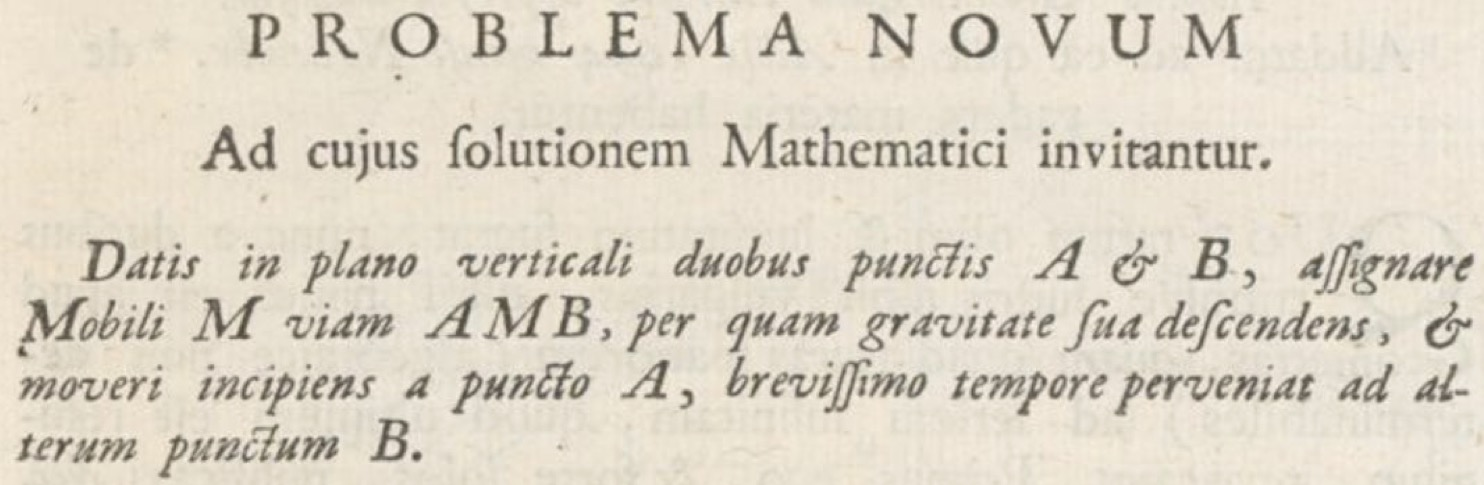
\includegraphics[width=0.8\textwidth]{chapters/020-variation/images/latein.jpg}
\end{center}
Zu deutsch:
\begin{quote}
Neue Aufgabe, zu deren Lösung die Mathematiker eingeladen werden.
Gegeben zwei Punkte $A$ und $B$ in einer vertikalen Ebene, finde
die Bahn $AMB$ eines Punktes $M$, der unter der Wirkung seines
Gewichtes in kürzester Zeit vom Punkt $A$ zum anderen Punkt $B$ absteigt.
\end{quote}
Die Situation der Aufgabenstellung ist in
Abbildung~\ref{buch:variation:fig:brachistochronenproblem}
dargestellt.
Bernoulli hat als Lösung gefunden, dass die Kurve eine Ausschnitt
aus einer Zykloide (in der Abbildung grau) sein muss.
Seine Lösung beruhte auf der Beobachtung, dass sich das Problem analog
zu einem Lichtausbreitungsproblem ist, für welches Fermat bereits
eine Lösung gefunden hat.

Da die Reibung vernachlässigt wird, ist die Energie des Massepunktes
erhalten.
Sie setzt sich aus der potenziellen und der kinetischen Energie
zusammen.
Die potenzielle Energie ist $-mgy$, die kinetische Energie ist
$\frac12mv^2$.
Die Energieerhaltung wird daher zu
\[
E=\frac12mv^2-mgy
\qquad\Rightarrow\qquad
v
=
\sqrt{2g}\!\sqrt{\frac{E}{gm}+y}
=
\!\sqrt{2(C+y)}.
\]
Durch Wahl einer anderen Zeiteinheit kann die Gleichung noch weiter
vereinfacht zu
\(
v = \sqrt{C+y}
\)
vereinfacht werden.
Gesucht ist also die zeitlich kürzeste Bahn eines Teilchens, 
dessen Geschwindigkeit auf bekannte Art $v(y)$ von der vertikalen
Koordinate abhängt.

%
% Das Fermat-Problem
%
\subsection{Das Fermat-Prinzip}
Bereits Fermat hat erkannt, dass das Brechnungsgesetz von Snellius
als Lösung eines Extremalproblems verstanden werden kann.

\begin{satz}[Fermat]
Sie $c/n_i$ die Geschwindigkeit, mit der sich Licht im Medium $M_i$
ausbreitet.
Ein Lichtstrahl von $A_1$ nach $A_2$ geht durch denjenigen Punkt $B$ 
auf der Grenzfläche zwischen den Medien, für den sich die Sinus der
Winkel $\alpha_i$ zwischen den Strahlen und der Normalen zur Grenzfläche
umgekehrt wie die $n_i$ verhalten, wenn also das Brechungsgesetz
\[
\frac{\sin\alpha_1}{\sin\alpha_2}
=
\frac{n_2}{n_1}
\]
gilt.
\end{satz}

\begin{proof}
Ohne der Beschränkung der Allgmeinheit können wir auf die Betrachtung
einer Ebene beschränken, die die beiden Punkte $A_i$ enthält und senkrecht
auf der Grenzfläche steht.
Wir dürfen weiter annehmen, dass die $x$-Achse in der Grenzfläche liegt 
und die Punkte $A_i$ die Koordinaten $(x_i,y_i)$ und der Punkt $B$ die
Koordinaten $(x,0)$ hat.
Es ist derjenige Punkt $x$ zu bestimmen, für den die Lichtzeit entlang 
des Pfades $A_1BA_2$ minimal wird.
Diese Zeit ist
\begin{align*}
t
&=
\frac{\overline{A_1B}}{c/n_1}
+
\frac{\overline{BA_2}}{c/n_2}
\\
ct
&=
n_1\overline{A_1B}
+
n_2\overline{A_2B}
\\
&=
n_1\!\sqrt{(x-x_1)^2 + y_1^2}
+
n_2\!\sqrt{(x_2-x)^2 + y_2^2}
\end{align*}
Das Minimum wird bei einer Nullstelle der Ableitung nach $x$ gefunden,
also bei einer Lösung der Gleichung
\begin{align*}
0
&=
n_1\frac{2(x_1-x)x}{\sqrt{(x_1-x)^2+y_1^2}}
+
n_2\frac{-2(x-x_2)x}{\sqrt{(x_2-x)^2+y_2^2}}.
\intertext{Indem man den zweiten Term auf der rechten Seite auf die linke
Seite bringt und durch $x$ dividiert, erhält man}
n_1
\frac{x_1-x}{\sqrt{(x_1-x)^2+y_1^2}}
&=
n_2
\frac{x-x_2}{\sqrt{(x_2-x)^2+y_2^2}}.
\end{align*}
Der Nenner ist auf beiden Seiten die Hypothenuse eines rechtwinkligen
Dreiecks, welches als Ankathete die Normale zur Grenzfläche hat.
Der Zähler ist die Gegenkathete des Winkels $\alpha_i$ zwischen der
Hypothenuse und der Normalen.
Daher ist der Quotient der Sinus des Winkels oder
\begin{equation}
n_1 \sin\alpha_1 = n_2 \sin\alpha_2.
\label{buch:variation:problem:eqn:snelliusinvariante}
\end{equation}
Die Gleichung~\eqref{buch:variation:problem:eqn:snelliusinvariante}
ist gleichbedeutend mit dem Brechungsgesetz
\[
\frac{\sin\alpha_1}{\sin\alpha_2}
=
\frac{n_2}{n_1}
\]
von Snellius.
\end{proof}

Der Satz von Fermat etabliert das Brechungsgsetz also Lösung eines
Extremalproblems.
Die Natur wählt für einen Lichtstrahl den zeitlich kürzesten Weg.
Der Beweis des Satzes von Fermat zeigt, dass entlang des Lichtstrahls
an jeder Grenzfläche zwischen Medien die Bedingung
\eqref{buch:variation:problem:eqn:snelliusinvariante}
erfüllt.
Wenn die optische Dichte $n$ eine Funktion von $n(y)$ ist, dann
wird der Lichtstrahl nicht nur in diskreten Punkten geknickt, sondern
entlang des ganzen Strahles gekrümmt.
Folgt der Strahl der Kurve $x(y)$, die mit der vertikalen den Winkel
$x'(y) = \tan\alpha(y)$ einschliesst.
Damit lässt sich auch die Sinus-Funktion ausdrücken, es gilt
\[
\sin\alpha(y)
=
\frac{x'(y)}{\pm\!\sqrt{x'(y)^2+1}}.
\]
Aus der Form~\eqref{buch:variation:problem:eqn:snelliusinvariante}
des Brechungsgesetztes wird dann die Gleichung
\begin{equation}
n_1\sin\alpha(y)
=
\frac{n_1(y)x'(y)}{\pm\!\sqrt{x'(y)^2+1}}
=
\operatorname{const}
\qquad\Rightarrow\qquad
\frac{n_1(y)^2x'(y)^2}{x'(y)^2+1}=C.
\label{buch:variation:eqn:fermatdgl}
\end{equation}
Dies ist eine Differentialgleichung für die Funktion $x(y)$.
Sie kann auch in die Form
\[
x'(y)^2
=
\frac{C}{(n_1(y)^2-C)}
\]
gebracht werden.

%
% Das Brachistochronenproblem als Lichtausbreitungsproblem
%
\subsubsection{Das Brachistochronenproblem als Lichtausbreitungsproblem}
Das Fermat-Prinzip besagt, dass ein Lichtstrahl, der sich in einem Medium
mit der Geschwindigkeit $c/n(y)$ ausbreitet, die Gleichung 
\eqref{buch:variation:eqn:fermatdgl} erfüllt.
Beim Brachistochronenproblem ist die Geschwindigkeit $v(y)=\!\sqrt{C-y}$ und 
damit $n(y) = c/\!\sqrt{C-y}$.
Eine Brachistochrone ist also eine Kurve, die die aus
\eqref{buch:variation:eqn:fermatdgl} folgende Gleichung
\begin{equation}
\frac{x'(y)^2}{(1+x'(y)^2)(C-y)} = K
\label{buch:variation:problem:eqn:bernoullidgl}
\end{equation}
erfüllen.

%
% Die Bernoullische Lösung
%
\subsubsection{Die Bernoullische Lösung}
Bernoulli hat gefunden, dass die Brachistochrone ein Zykloidenbogen ist.
Dies lässt sich dadurch verifizieren, dass man die Parametrisierung
einer Zykloide in die
Gleichung~\eqref{buch:variation:problem:eqn:bernoullidgl}
einsetzt.
Die Zykloide hat die Parametrisierung
\[
\left.
\begin{aligned}
x &= r(\varphi - \sin\varphi) 
\\
y &= r(1-\cos\varphi)
\end{aligned}
\right\}
\quad
\text{mit der Ableitung}
\quad
\left\{
\begin{aligned}
\dot{x}(\varphi) &= r(1-\cos\varphi)\\
\dot{y}(\varphi) &= r\sin\varphi
\end{aligned}
\right.
\]
für $\varphi\in\mathbb{R}$.
Die Ableitung ist
\[
x'(y)
=
\frac{\dot{x}(\varphi)}{\dot{y}(\varphi)}
=
\frac{1-\cos\varphi}{\sin\varphi}.
\]
Eingesetzt in \eqref{buch:variation:problem:eqn:bernoullidgl}
wird daraus
\[
\frac{\dot{x}(\varphi)^2}{
(\dot{y}(\varphi)^2 +\dot{x}(\varphi)^2)
(C-r(1-\cos\varphi))
}
=
\frac{(1-\cos\varphi)^2}{
((1-\cos\varphi)^2+\sin^2\varphi)
(C-r+r\cos\varphi)
}
=
K.
\]
Ausmultiplizieren im Nenner ergibt
\[
\frac{(1-\cos\varphi)^2}{
(1-2\cos\varphi+\cos^2\varphi+\sin^2\varphi)
(C-r+r\cos\varphi)
}
=
\frac{1-\cos\varphi}{
2(C-r+r\cos\varphi)
}
\]

%
% Das Brachistochronenproblem als Variationsproblem
%
\subsection{Das Brachistochronenproblem als Variationsproblem
\label{buch:variation:problem:subsection:variationsproblem}}
Die Bernoullische Lösung des Brachistochronenproblems verwendet die
Analogie zum Fermat-Prinzip.
Eine solche Analogie ist nur selten möglich, daher soll das Problem
jetzt in eine Form gebracht werden, in die auch viele ähnliche
Optimierungsproblem gebracht werden können.

Wir erinnern daran, dass die Geschwindigkeit des Massepunktes durch
$v(y)=\sqrt{C-y}$ gegeben ist.
Damit lässt sich die Zeit berechnen, die der Massepunkt entlang der
Lösungskurve braucht, wenn man diese als Funktion $y(x)$ mit beschreibt.
Die Punkte $A$ und $B$ sollen die $x$-Koordinaten $a$ bzw.~$b$ haben.
Für das Kurvenstück zwischen den $x$-Koordinaten $x$ und $x+\Delta x$
braucht der Massepunkt die Zeit
\[
\frac{ \sqrt{\Delta x^2 + \Delta y^2} }{v(y)}
=
\frac{ \sqrt{1 + y'(x)^2} }{ v(y) } \Delta x.
\]
Die Zeit ist das Integral
\begin{equation}
t
=
\int_a^b \frac{\sqrt{1+y'(x)^2}}{v(y(x))}\,dx
=
\int_a^b \sqrt{\frac{1+y'(x)^2}{C-y(x)}}\,dx.
\label{buch:variation:problem:eqn:brachint}
\end{equation}
Der Integrand auf der rechten Seite hängt nur von den Funktion $y(x)$
und $y'(x)$ ab.
Dies kommt vor allem daher, dass die Geschwindigkeit nur von $y$ abhängt,
nicht auch noch von $x$.
Im Allgemeinen wird man also davon ausgehen müssen, dass der Integrand
auch noch von $x$ abhängt.
Die Variationsrechnung befasst sich mit Problemen, in denen Funktionen
gefunden werden müssen, die ein Integral wie das in
\eqref{buch:variation:problem:eqn:brachint}
minimiert oder maximiert werden müssen.

\begin{definition}[Lagrange-Funktion des Brachistochronenproblems]
Die Lagrange-Funk\-tion des Brachistochronenproblems ist der
Integrand des Integrals
\eqref{buch:variation:problem:eqn:brachint},
\index{Lagrange-Funktion}%
also die Funktion
\[
L(x,y,y')
=
\sqrt{\frac{1+y^{\prime 2}}{C-y}}.
\]
\end{definition}

%
% Funktionale
%
\subsection{Funktionale
\label{buch:variation:problem:subsection:funktionale}}
Die Variationsrechnung löst Optimierungsproblem, die von einer
Funktion abhängen.
Um dies mathematisch präzis zu fassen, ist zunächst nötig, die Menge
der in Frage kommenden Funktionen so einzuschränken, dass die interessierende
Grösse überhaupt wohldefiniert ist.

%
% Vektorräume
%
\subsubsection{Vektorräume}
Zunächst sind die gemeinsamen algebraischen Eigenschaften zu charakterisieren,
die wir von den für unsere Untersuchungen zweckmässigen Funktionenmengen
erwarten.

\begin{definition}[Vektorraum]
Ein Vektorraum über den reellen Zahlen $\mathbb{R}$ ist einem Menge $V$ mit
zwei Operationen, der Addition und der Multiplikation mit Skalaren
\begin{align*}
    +\colon V\times V         &\to V : (u,v)\mapsto u+v
&
\cdot\colon \mathbb{R}\times V&\to V : (\lambda,v) \mapsto\lambda v
\end{align*}
mit den folgenden Eigenschaften.
\begin{enumerate}
\item
Es gelten die Assoziativgesetze
\begin{align*}
(u+v)+w&=u+(v+w)&&\text{für alle $u,v,w\in V$}\\
(\lambda \mu)v&=\lambda(\mu v)&&\text{für alle $\lambda,\mu\in\mathbb{R},\;v\in V$.}
\end{align*}
\item
Es gibt einen Vektor $0\in V$ mit der Eigenschaft $0+v=v$ für alle
Vektoren $v\in V$.
\item
Zu jedem Vektor $v\in V$ gibt es den entgegengesetzten Vektor $-v\in V$
mit der Eigenschaft, dass $-v+v=0$ ist.
\item
Die Addition von Vektoren ist kommutativ: $u+v=v+u$ für alle $u,v\in V$.
\item
Es gelten die Distributivgesetze 
\begin{align*}
(\lambda + \mu) v &= \lambda v + \mu v
	&\quad\text{für alle $\lambda,\mu\in\mathbb{R},\;v\in V$}\\
\lambda(u+v)      &= \lambda u + \lambda v
	&\quad\text{für alle $\lambda\in\mathbb{R},\;u,v\in V$}
\end{align*}
\end{enumerate}
\end{definition}

Die Mengen $\mathbb{R}^n$ erfüllen die genannten Eigenschaften, sind
also Vektorräume.
Die Definition eines Vektorraums ist aber viel allgemeiner, insbesondere
gehören dazu auch Mengen von Funktionen.
Damit wird es möglich, die Berechnungen in $\mathbb{R}^n$ auf Funktionen
auszudehnen.
Zum Beispiel bilden die stetigen Funktionen auf einem Intervall einen
Vektorraum, wie das folgende Beispiel zeigt.

\begin{beispiel}
Die Menge
\[
C([a,b])
=
\{f\colon[a,b]\to\mathbb{R}\mid \text{$f$ ist stetig}\}
\]
der stetigen Funktionen bildet einen Vektorraum.
Die Operationen sind die punktweise Addition von Funktionen und die
Multiplikation der Werte mit Skalaren, für $f,g\in C([a,b])$ und
$\lambda\in \mathbb{R}$ ist
\begin{align*}
(f+g)(x) &= f(x)+g(x)
&&\text{und}&
(\lambda f)(x) &= \lambda f(x).
\end{align*}
Entscheidend ist, dass die Addition von Funktionen und die Multiplikation
mit Skalaren nicht aus der Menge herausführt.
Tatsächlich wird in der Analysis gezeigt, dass die Summe stetiger Funktionen
wieder stetig ist und dass die Funktion $x\mapsto \lambda f(x)$ stetig,
wenn $f$ stetig ist.
Die übrigen Eigenschaften sind ebenfalls erfüllt, da sie bereits für die
Funktionswerte erfüllt sind.
\end{beispiel}

%
% Norm und Grenzwerte
%
\subsubsection{Norm und Grenzwerte}
Um Analysis zu betreiben, muss man ausdrücken können, dass eine Folge
von Funktionen konvergiert.
Dazu ist ein Abstandsbegriff zwischen Funktionen nötig.

\begin{definition}[Norm, normierter Raum]
Eine {\em Norm} auf einem Vektorraum $V$ ist eine Abbildung
\index{Norm}%
$\|\cdot\|\colon V\to\mathbb{R}^+_0$ mit nichtnegativen reellen Werten
und den folgenden Eigenschaften
\begin{itemize}
\item Definitheit: $\|v\|\ge 0$ für $v\in V$ mit Gleichheit 
genau dann, wenn $v=0$.
\index{Definitheit}%
\item Absolute Homogenität: Für alle Vektoren $v\in V$ und
\index{Homogenität}%
$\lambda\in\mathbb{R}$ gilt $\|\lambda v\| = |\lambda|\, \|v\|$.
\item Dreiecksungleichung: für alle Vektoren $u,v\in V$ gilt
\index{Dreiecksungleichung}%
$\|u+v\|\le \|u\|+\|v\|$.
\end{itemize}
Ein {\em normierter Raum} ist ein Vektorraum mit einer Norm.
\index{normierter Raum}%
\end{definition}

\begin{beispiel}
Der Vektorraum der stetigen Funktionen kann mit der Supremum-Norm
\[
\|f\| = \sup_{x\in[a,b]} |f(x)|
\]
zu einem normierten Raum gemacht werden.
Die Definitheit ist durch die Definition offensichtlich sichersgtellt.
Für $\|\lambda f\|$ finden wir
\[
\|\lambda f\|
=
\sup_{x\in[a,b]} |\lambda f(x)|
=
|\lambda|\,
\sup_{x\in[a,b]} |f(x)|
=
|\lambda|\, \|f\|,
\]
was die Homogenität zeigt.
Die Dreiecksungleichung folgt aus
\begin{align*}
\|f+g\|
&=
\sup_{x\in[a,b]} |f(x)+g(x)|
\\
&\le
\sup_{x\in[a,b]} (|f(x)|+|g(x)|)
\\
&\le
\sup_{x\in[a,b], y\in[a,b]} (|f(x)|+|g(y)|)
\\
&=
\sup_{x\in[a,b]} |f(x)|
+
\sup_{y\in[a,b]} |g(y)|
=
\|f\| + \|g\|.
\qedhere
\end{align*}
\end{beispiel}

Mit einer Norm ist es jetzt möglich, die Konvergenz von Folgen und den
Begriff des Grenzwertes zu definieren.

\begin{definition}[Cauchy-Folge, Grenzwert]
Eine Folge $(x_n)_{n\in\mathbb{N}}$ in $V$ in einem normierten Raum $V$
mit der Norm $\|\cdot\|$
heisst eine Cauchy-Folge, wenn es für jedes $\varepsilon>0$ eine
\index{Cauchy-Folge}%
$N\in \mathbb{N}$ gibt derart, dass
\[
\| x_n - x_m \| < \varepsilon
\quad\forall n,m\ge N.
\]
Der Vektor $x\in V$ heisst {\em Grenzwert} der Folge $(x_n)_{n\in\mathbb{N}}$,
\index{Grenzwert}%
wenn es zu jedem $\varepsilon > 0$ ein $N\mathbb{N}$ gibt derart, dass
\[
\|x_n-x\| < \varepsilon 
\quad\forall n\ge N.
\]
Die Folge $(x_n)_{n\in\mathbb{N}}$  in $V$ heisst {\em konvergent}, wenn
\index{konvergent}%
$x$ der Grenzwert von $(x_n)_{n\in\mathbb{N}}$ ist.
\end{definition}

Der durch die Supremum-Norm definierte Konvergenzbegriff ist die gleichmässige
Konvergenz.
Zur Erinnerung:
Eine Folge $f_n$ von Funktionen heisst gleichmässig konvergent gegen die
Funktion $f$, wenn es zu jedem
$\varepsilon >0$ ein $N\in\mathbb{N}$ gibt derart, dass
\[
|f_n(x) - f(x)|<\varepsilon\quad\forall n>N\text{ und }x\in [a,b].
\]
Die Supremum-Norm ist
\[
\|f_n(x) - f(x)\|
=
\sup_{x\in[a,b]} |f_n(x)-f(x)| < \varepsilon
\]
für alle $n>N$.
Dies ist genau die Konvergenz in der Norm $\|\cdot\|$.
Aus der Analysis ist bekannt, dass eine gleichmässig konvergente 
Funktionenfolge gegen eine stetige Funktion konvergiert.

\begin{definition}[Banach-Raum]
Ein normierter Raum $V$ heisst ein {\em Banach-Raum},
\index{Banach-Raum}%
wenn jede Cauchy-Folge in $V$ einen Grenzwert hat.
\end{definition}

\begin{beispiel}
Die Menge $C^1([0,2])$
der stetigen Funktionen auf dem Intervall $[0,2]$ ist ein normierter
Raum mit der Norm
\[
\|f\|_1
=
\int_0^2 |f(x)|\,dx,
\]
die auch die $L^1$-Norm heisst.
\index{L1-Norm@$L^1$-Norm}%
Zunächst ist nachzuprüfen, dass dies tatsächlich eine Norm ist.
Die Definitheit und die Homogenität von $\|\cdot\|_1$ ist klar, nur
die Dreiecksungleichung erfordert etwas Arbeit.
Für Funktionen $f,g\in L^1([0,2])$ gilt
\begin{align*}
\|f+g\|_1
&=
\int_0^2 |f(x)+g(x)|\,dx
\\
&\le 
\int_0^2 |f(x)|+|g(x)|\,dx
=
\int_0^2 |f(x)|\,dx
+
\int_0^2 |g(x)|\,dx
=
\|f\|_1+\|g\|_1,
\end{align*}
was die Dreeicksungleichung beweist.

Eine Cauchy-Folge in der $L^1$-Norm muss aber nicht unbedingt einen
stetigen Grenzwert haben.
Die Funktionen
\(
f_n(x) =
\begin{cases}
x^n&\quad x< 1\\
1&\quad x\ge 1
\end{cases}
\)
haben die $L^1$-Norm
\begin{align*}
\|f_n-f_m\|_1
=
\int_0^2 |f_n(x)-f_m|\,dx
\\
&=
\biggl|\int_0^1 x^n-x^m\,dx\biggr|
=
\biggl[
\biggl|
\frac{1}{n+1}x^{n+1}
-
\frac{1}{m+1}x^{m+1}
\biggr|
\biggr]_0^1
\\
&=
\biggl|
\frac{1}{n+1}
-
\frac{1}{m+1}\biggr|.
\end{align*}
Wegen
\[
\|f_n-f_m\|_1
<\varepsilon
\]
für $n,m>2/\varepsilon$ ist $f_n$ eine Cauchy-Folge in $L^1$.
In $L^1$ konvergiert die Folge $f_n$ gegen die Funktion
\[
f(x)
=
\begin{cases}
0&\quad x< 1\\
1&\quad x\ge 1.
\end{cases}
\]
Diese Funktion ist aber nicht stetig, da sie bei $x=1$ einen
Sprung hat.
Bezüglich der $L^1$-Norm ist $C^1([a,b])$ als im Allgemeinen
kein Banach-Raum.
\end{beispiel}

%
% Stetige und differenzierbare Funktionen
%
\subsubsection{Stetige und differenzierbare Funktionen}
Mit der Norm lässt sich auch die Stetigkeit von Abbildungen zwischen
normierten Räumen definieren.

\begin{definition}[Stetigkeit]
Eine Funktion $f\colon U\to V$ zwischen normierten Räumen heisst
{\em stetig im Punkt} $x\in U$, wenn es zu jedem $\varepsilon > 0$
\index{stetig in einem Punkt}%
ein $\delta > 0$
gibt derart, dass
\(
\|f(x)-f(y)\| < \delta
\)
wenn
\(
\|x-y\|<\varepsilon
\).
Eine Funktion $f\colon U\to V$ heisst {\em stetig}, wenn sie in
jedem Punkt von $U$ stetig ist.
\end{definition}

Das Bild einer Folge $x_n\in U$, die gegen $x_0\in U$ konvergiert,
ist eine Folge $f(x_n)$ in $V$.
Man sagt, $y\in V$ sei der Grenzwert von $f(x)$ für $x\to x_0$,
wenn $f(x_n)$ für jede solche Folge $x_n$ gegen $y$ konvergiert.
Der Grenzwert wird auch
\[
\lim_{x\to x_0} f(x)
=
y
\]
geschrieben.
Stetige Funktionen zeichnen sich wie in der Analysis der Funktionen
einer Variablen dadurch aus, dass der Grenzwert der Werte der Funktion
auf einer konvergenten Folge mit dem Funktionswert des Grenzwertes
übereinstimmt.

\begin{satz}
Eine Funktion $f\colon U\to V$ ist genau dann stetig im Punkt $x\in U$,
wenn für jede Folge $x_n$ in $U$ mit Grenzwert $x$ die Folge $f(x_n)$
konvergent ist und
\[
\lim_{n\to\infty} f(x_n) = f(x).
\]
Eine lineare Funktion $f\colon U\to V$ ist genau dann stetig,
wenn für jede Nullfolge $x_n$ in $U$ 
\[
\lim_{n\to \infty} f(x_n) = 0
\]
gilt.
\end{satz}

\begin{definition}
Eine Funktion $f\colon U\to V$ zwischen normierten Räumen heisst
differenzierbar im Punkt $x\in U$ wenn es eine lineare Funktion
$Df(x_0)\colon U\to V$ gibt derart, dass
\[
f(x+v) =f(x) + Df(x_0)\cdot v + o(v),
\]
wobei $o(v)$ bedeutet, dass für diese Funktion
\[
\frac{o(v)}{|v|}\to 0
\quad\text{für $v\to 0$}
\]
gilt.
\end{definition}

Funktionen auf einem Vektorraum mit reellen Werten weren auch
{\em Funktionale} genannt.
\index{Funktional}
Vor dem 20.~Jahrhundert wurde häufig ein Untersschied zwischen
Funktionen von endlich vielen reellen Variablen und Funktionen
von einem unendlichdimensionalen Vektorraum gemacht.
Die Entwicklungen dieses  Abschnittes haben gezeigt, dass eine
solche Unterscheidung nicht gerechtfertigt ist.
Es ist lediglich notwendig, die Definitionen allgemein genug zu
fassen und sich jederzeit über die Funktionenmenge und die zu
verwendende Norm Rechenschaft abzulegen.


%
% 2-fundamtenallemma.tex
%
% (c) 2023 Prof Dr Andreas Müller
%
\section{Das Fundamentallemma
\label{buch:variation:section:fundamentallemma}}
\kopfrechts{Das Fundamentallemma}
Im Fall des endlichdimensionalen Extremalproblems ist aus der
Forderung, dass alle Richtungsableitung verschwinden müssen, 
die Bedingung geworden, dass
\[
v\cdot\grad f = 0
\]
sein muss für alle Vektoren $v\in\mathbb{R}^n$.
Wir haben daraus geschlossen, dass der Gradient $\grad f=0$
sein muss.
Wir hatten dies das endlichdimensionale Fundamentallemma genannt,
wegen $e_k\cdot \grad f = D_kf$ war es eine ziemliche Selbstverständlichkeit.
Bei der Lösung von Variationsproblemen, wo es nicht um endlichdimensionale
Vektoren und das Skalarprodukt, sondern um Funktionen und Integrale
geht, brauchen wir eine ähnliche Aussage für Funktionen.

%
% Positive glatte Funktionen mit kompaktem Träger
%
\subsection{Positive glatte Funktionen mit kompaktem Träger}
Die Aussage des Fundamentallemmas für endlichdimensionale Vektoren 
folgte sofort aus der Tatsache, dass es für jedes $k$ einen Vektor
$e_k$ gibt, der nur in der Koordinaten $k$ von $0$ verschieden ist.
Natürlich gibt es auch Funktionen, die nur in genau einem Punkt
von $0$ verschieden sind.
Eine solche Funktion ist aber im allgemeinen nicht differenzier-
oder integrierbar.
In diesem Abschnitt soll daher gezeigt werden, dass es unendlich
oft stetig differnzierbare Funktionen gibt, die nur in einem beliebig
kleinen vorgegebenen Intervall $\ge 0$ sind.

\begin{definition}[Träger]
Der {\em Träger} einer Funktion $f\colon X\to\mathbb{R}$ ist die Menge
\index{Träger}%
\[
\supp f = \{ x\in X\mid f(x)\ne \}.
\]
\end{definition}

Gesucht ist also eine beliebig oft stetig differenzierbare Funktion,
deren Träger in einem vorgegebenen Intervall $[a,b]$ enthalten ist.
Wir konstruieren so eine Funktion in zwei Schritten.

\input{chapters/020-variation/fig/f.tex}

\begin{satz}
\label{buch:variation:fundamentallemma:satz:glatt}
Die Funktion
\[
f(x)
=
\begin{cases}
e^{-1/x}&\qquad x>0\\
0&\qquad x\le 0
\end{cases}
\]
(siehe auch Abbildung~\ref{buch:variation:fundamentallemma:fig:glatt})
ist beliebig oft stetig differenzierbar.
\end{satz}

\begin{proof}
Es ist klar, dass die Funktion $f$ beliebig oft stetig differenzierbar
ist in jedem Punkt $x\ne 0$.
Es ist also nur nachzuweisen, dass $f(x)$ im Punkt $0$ beliebig
oft stetig differenzierbar ist.

Die ersten drei Ableitungen von $f(x)$ sind
\begin{align}
f'(x) &= \frac{1}{x^2} f(x)
\label{buch:variation:fundamentallemma:eqn:f1}
\\
f''(x) &= \frac{1-2x}{x^4}f(x)
\notag
\\
f'''(x) &= \frac{6x^2-6x+1}{x^6}f(x).
\notag
\end{align}
Daraus lässt sich die Vermutung ableiten, dass
\begin{equation}
f^{(n)}(x)
=
\frac{p_{n-1}(x)}{x^{2n}} f(x)
\label{buch:variation:fundamentallemma:eqn:fabl}
\end{equation}
ist, wobei $p_k(x)$ ein Polynom vom Grad $k$ ist.
Wir beweisen diese Vermutung mit Hilfe von vollständiger Induktion.
Die Induktionsverankerung für die $0$-te Ableitung ist trivial.

Wir nehmen jetzt im Sinne der Induktionsannahme an, dass die $n$-te
Ableitung die Form \eqref{buch:variation:fundamentallemma:eqn:fabl}
hat.
Wir müssen zeigen, dass dann auch $f^{(n+1)}(x)$ diese Form hat.
Dazu berechnen wir
\begin{align}
f^{(n+1)}(x)
&=
\frac{d}{dx}
\frac{p_n(x)}{x^{2n}} f(x)
\notag
\\
&=
\frac{p_n'(x)}{x^{2n}} f(x)
-2n
\frac{p_n(x)}{x^{2n+1}} f(x)
+
\frac{p_n(x)}{x^{2n}} f'(x).
\notag
\intertext{Mit der ersten Ableitung
\eqref{buch:variation:fundamentallemma:eqn:f1} wird dies zu}
&=
\frac{p_n'(x)}{x^{2n}} f(x)
-2n
\frac{p_n(x)}{x^{2n+1}} f(x)
+
\frac{p_n(x)}{x^{2n}} \frac{1}{x^2}f(x)
\notag
\\
&=
\frac{x^2p_n'(x) -2nxp_n(x)+p_n(x)}{x^{2n+2}} f(x).
\label{buch:variation:fundamentallemma:eqn:induktionsschritt}
\end{align}
Die Ableitung $p_n'(x)$ ist ein Polynom vom Grad $n-1$ und damit
ist $x^2p_n'(x)$ ein Polynom vom Grad $n+1$.
Ebenso ist $xp_n(x)$ ein Polynom vom Grad $n+1$ während
$p_n(x)$ ein Polynom vom Grad $n$ ist.
Der Zähler von
\eqref{buch:variation:fundamentallemma:eqn:induktionsschritt}
ist
\[
p_{n+1}(x)
=
x^2p_n'(x)+(1 -2nx)p_n(x),
\]
ein Polynom vom Grad $n+1$.
Damit ist der Induktionsschritt erfolgreich und die Behauptung betreffend
die Form von $f^{(n)}(x)$ ist bewiesen.

Es ist jetzt nur noch zu zeigen, dass der Grenzwert von $f^{(n)}(x)$
für $x\to 0+$ verschwindet.
Da das Polynom $p_n(x)$ stetig ist, folgt
\[
\lim_{x\to 0}
f^{(n)}(x)
=
\lim_{x\to 0}\frac{p_n(x)}{x^{2n}}f(x)
=
p_n(0) \lim_{t\to\infty} t^{2n} e^{-t}
=
0.
\]
Damit ist die beliebige stetige Differenzierbarkeit an der Stelle
$x=0$ gezeigt.
\end{proof}

Die Funktion $f(x)$ von 
Satz~\ref{buch:variation:fundamentallemma:satz:glatt} 
erfüllt noch nicht die Forderung, dass sie nur in einem vorgegebenen
Intervall von $0$ verschieden ist.

\input{chapters/020-variation/fig/g.tex}

\begin{satz}
\label{buch:variation:fundamentallemma:satz:gab}
Sei $f(x)$ die Funktion von
Satz~\ref{buch:variation:fundamentallemma:satz:glatt}.
Dann ist
\[
g_{a,b}(x)
=
f(x-a) f(b-x)
\]
eine unendlich oft stetig differenzierbare, nichtnegative Funktion mit Träger
$\supp g_{a,b}=(a,b)$.
\end{satz}

Die Funktionen $g_{a,b}(x)$ sind beliebig oft differenzierbar und nur im
Intervall $[a,b]$ von $0$ verschieden und sogar positiv.
Weil sie stetig sind, sind sie auch integrierbar, man kann also das
Integral über $\mathbb{R}$ berechnen und die Funktion damit normieren.
Die neue Funktion
\[
\frac{1}{N}
\tilde{g}_{a,b}(x)
\qquad\text{mit}\;
N
=
\int_{-\infty}^{\infty}g_{a,b}(x)\,dx
=
\int_a^b g_{a,b}(x)\,dx
\]
ist immer noch beliebig oft stetig differenzierbar und hat zusätzlich die
Eigenschaft
\[
\int_{-\infty}^{\infty}
\tilde{g}_{a,b}(x)\,dx
=
\int_a^b
\tilde{g}_{a,b}(x)\,dx
=
1.
\]
Wir formulieren dieses Resultat als Satz.

\begin{satz}
\label{buch:variation:satz:gabeins}
Zu jedem Intervall $[a,b]$ gibt es eine beliebig oft stetig
differenzierbare Funktion $g(x)$, genau das Intervall $[a,b]$
als Träger hat und deren Integral über $[a,b]$ den Wert $1$ hat.
\end{satz}

%
% Das Fundamentallemma
%
\subsection{Das Fundamentallemma}
Mit der Funktion $g_{a,b}(x)$ von
Satz~\ref{buch:variation:fundamentallemma:satz:gab}
lässt sich jetzt das Fundamentallemma in der folgenden Form
leicht beweisen.

\begin{satz}[Fundamentallemma]
\label{buch:variation:fundamentallemma:satz:fundamentallemma}
Wenn für die stetige Funktion $f\colon[a,b]\to\mathbb{R}$ 
\begin{equation}
\int_a^b f(x)\varphi(x)\,dx = 0
\label{buch:variation:fundamentallemma:eqn:fundamentalbed}
\end{equation}
gilt für jede beliebig oft stetig differenzierbare Funktion $\varphi(x)$ 
dann ist $f(x)=0$.
Das Resultat gilt selbst dann, wenn
\eqref{buch:variation:fundamentallemma:eqn:fundamentalbed}
nur für beliebig oft stetig differenzierbare Funktionen $\varphi(x)$ 
gilt, die ausserdem an den Intervallenden verschwinden:
$\varphi(a)=\varphi(b)=0$.
\end{satz}

\begin{proof}
Wir zeigen mit Hilfe eines Widerspruchs, dass es keinen Punkt $x_0\in[a,b]$
geben kann, für den $f(x_0)\ne 0$ ist.
Dazu nehmen wir also an, dass $f(x_0)\ne 0$ ist.
Falls $f(x_0)<0$ ist, ersetzen wir $f$ durch $-f$, 
die Bedingung
\eqref{buch:variation:fundamentallemma:eqn:fundamentalbed}
ändert sich dadurch nicht.
\input{chapters/020-variation/fig/fundamentallemma.tex}
Wir dürfen daher annehmen, dass $f(x_0)>0$ ist
(Abbildung~\ref{buch:variation:fundamentallemma:fig:beweis}).
Da $f$ stetig ist, gibt es ein Intervall $[x_0-\varepsilon,x_0+\varepsilon]$
derart, dass $f(x)> \frac12 f(x_0)$ für
$x\in[x_0-\varepsilon,x_0+\varepsilon]$ gilt.
Dann gilt für das Integral
\[
\int_a^b
f(x)
g_{x_0-\varepsilon,x_0+\varepsilon} (x)
\,dx
>
\frac{f(x_0)}{2}
\int_a^b
g_{x_0-\varepsilon,x_0+\varepsilon} (x)
\,dx
>
0
\]
im Widerspruch zur Bedingung
\eqref{buch:variation:fundamentallemma:eqn:fundamentalbed}.
Der Widerspruch zeigt, dass $f(x)=0$ sein muss.
\end{proof}

%
% Skalarproduktformulierung des Fundamentallemmas
%
\subsection{Skalaproduktformulierung des Fundamentallemmas}
Die Richtungsableitung einer Funktion endlich vieler Variablen 
konnte als Skalarprodukt mit dem Gradienten geschrieben werden und
das Fundamentallemma hat besagt, dass der Gradient verschwindet,
wenn alle Richtungsableitungen verschwinden.
Diese Schlussweise ist auch für Funktionen möglich, wenn man Funktionen
ein Skalarprodukt definieren kann.

\begin{definition}[$L^2$-Skalarprodukt]
Das {\em Skalarprodukt} zweier quadratintegrierbarer Funktion $f$ und $g$
auf dem Intervall $[a,b]$ ist definiert durch
\[
\langle f,g\rangle
=
\int_a^b f(x)g(x)\,dx.
\]
\end{definition}

\begin{satz}[Fundamentallemma, Skalarproduktform]
Wenn für eine stetige Funktion $f\colon[a,b]\to\mathbb{R}$ das Skalarprodukt
\[
\langle f,\varphi\rangle = 0
\]
ist für jede unendlich oft differenzierbare Funktion $\varphi$ auf dem
Intervall $[a,b]$, dann ist $f=0$.
\end{satz}



%
% 3-eulerlagrange.tex
%
% (c) 2023 Prof Dr Andreas Müller
%
\section{Die Euler-Lagrange Differentialgleichung
\label{buch:variation:section:eulerlagrange}}
\kopfrechts{Die Euler-Lagrange Differentialgleichung}
Das Neuartige an der Aufgabenstellung des Brachistochronenproblems
war, dass eine Funktion gesucht war, so dass ein damit gebildetes
Integral eine Minimaleigenschaft erfüllt.
Für die damalige Mathematik war die Aufgabe, eine Funktion zu finden,
nicht neu.
Die Theorie der Differentialgleichungen war bereits entwickelt,
Newton hat die Infinitesimalrechnung ja erfunden, um damit die
Bewegungsgleichungen der Physik zu formulieren und zu lösen.
In einer Differentialgleichung werden Werte und Ableitungen einer
Funktion an einer einzigen Stelle miteinander verbunden.
Etwas salop formuliert sagt die Differentialgleichung in jedem
Punkt, in welche Richtung und mit welcher Krümmung die Funktionskurve
weiter zu zeichnen ist.

Im Brachistochronenproblem tragen aber alle Werte der gesuchten
Funktion zum Integral bei, es scheint daher auf den ersten Blick
nicht möglich, das Problem durch schrittweise Konstruktion
``von Punkt zu Punkt'' der Lösungskurve zu konstruieren.

Bernoullis Lösung des Brachistochrononproblems beruht auf der
Beobachtung, dass sich die Bedinung für die schnellste Bahn
durch eine Bedingung ersetzen lässt, die in jedem einzelnen
Punkt ausgewertet werden kann.
Das von ihm verwendete Fermat-Prinzip wurde ursprünglich ebenfalls
als eine globale Eigenschaft eines Lichtstrahls formuliert.
Aus dem Fermat-Prinzip folgt aber das Brechungsgesetz, welches
sagt, dass die Richtung eines Strahls in einem Punkt genau dann
ändert, wenn sich dort auch der Brechungsindex der beiden Medien
ändert.
Das Fermat-Prinzip ist also ein Beispiel dafür, wie eine globale
Bedingung erfüllt werden kann, indem einer lokalen Regel in jedem
Punkt gefolgt wird.

Es ist das Verdienst von Euler und Lagrange, zu erkennen, dass diese
Übersetzung eines globalen Variationsproblems in ein lokales 
Problem immer möglich ist.
Es entsteht dabei die Euler-Lagrange-Differentialgleichung, welche
die Problemstellung auf die Lösung einer Differentialgleichung
reduziert.
Damit ist ein allgemein anwendbares Lösungsverfahren gefunden.
Zu einem Variationsproblem lässt sich immer eine Differentialgleichung
finden, welche die gesuchte Funktion als Lösung hat.

In diesem Abschnitt soll dieser indirekte Weg der Lösung von
Variationsaufgaben dargestellt werden.
Wir werden später zeigen, dass diese Vorgehensweise nicht immer
erfolgreich sein kann.
Zum Beispiel werden wir in Kapitel~\ref{buch:chapter:nichtdiff}
Variationsprobleme kennenlernen, deren Lösungskurven nicht
differenzierbar sind und daher auch nicht von einer Differentialgleichung
gefunden werden können.
Im Kapitel~\ref{buch:chapter:direkt} werden daher die sogenannten
direkten Methodn vorgestellt, die den Umweg über eine
Differentialgleichung vermeiden.

%
% Die Lagrange-Funktion
%
\subsection{Die Lagrange-Funktion
\label{buch:variation:eulerlagrange:subsection:lagrange-funktion}}
Wir betrachten Variationsproblem der folgenden Art.
Gesucht ist eine auf dem Intervall $[x_0,x_1]$ definirte
Funktion $y(x)$, die das Integral
\begin{equation}
I(y)
=
\int_{x_0}^{x_1}
F(x, y(x), y'(x))
\,dx
\label{buch:variation:eulerlagrange:eqn:funktional}
\end{equation}
maximiert oder minimiert.
Der Ausdruck~\eqref{buch:variation:eulerlagrange:eqn:funktional}
wird ein Funktional genannt.
Die Funktion
\[
F
\colon
\mathbb{R}\times
\mathbb{R}\times
\mathbb{R}
\to
\mathbb{R}
\]
von drei Variablen heisst die {\em Lagrange-Funktion}
des Funktionals \eqref{buch:variation:eulerlagrange:eqn:funktional}.

\begin{beispiel}
Die Lagrange-Funktion des Brachistochronenproblems ist
\[
F(x,y,y')
=
\sqrt{ \frac{1+y^{\prime 2}}{y} }.
\]
Die Funktion hängt nicht von $x$ ab, was bedeutet, dass eine
Verschiebung in $x$-Richtung die Form der Lösungsfunktion des
Variationsproblems nicht ändert.
\end{beispiel}

\begin{beispiel}
\label{buch:variation:eulerlagrange:beispiel:gerade}
Wir formulieren die Aufgabe, die kürzeste Verbindung der Punkte
$(x_0,y_0)$ und $(x_1,y_1)$ in einer Ebene zu finden, als Variationsproblem.
Die Länge einer Kurve $y(x)$ ist das Integral
\[
l(y)
=
\int_{x_0}^{x_1}
\sqrt{1+y'(x)^2}\,dx.
\]
Daraus lesen wir ab, dass die Lagrange-Funktion dieses Variationsproblems
\begin{equation}
F(x,y,y') = \sqrt{1+y^{\prime 2}}
\label{buch:variation:eulerlagrange:eqn:geradeL}
\end{equation}
ist.
Die Funktion hängt weder von $x$ noch von $y$ ab.
Dies ist auch zu erwarten, denn die Länge einer Kurve hängt nicht davon
ob, wo in der Ebene sie platziert ist.
Eine Verschiebung in $x$-Richtung würde das $x$-Argument ändern,
eine Verschiebung in $y$-Richtung die $y$-Werte.
Wäre $F$ von $x$ oder $y$ abhängig, könnte auch die Länge der Kurve
davon abhängen.
\end{beispiel}

%
% Euler-Lagrange_Differentialgleichung
%
\subsection{Euler-Lagrange-Differentialgleichung
\label{buch:variation:eulerlagrange:subsection:dgl}}
\input{chapters/020-variation/fig/variation0.tex}
Das Maximum oder Minimum einer Funktionen mehrere Variablen wurde
gefunden, indem die Richtungsableitung berechnet und $=0$ gesetzt
wurde.
Um die Funktion zu bestimmen, die ein Funktional $I(y)$ zu einem
Maximum oder Minimum macht, versuchen wir, die Idee der Richtungsableitung
für ein Funktional nachzuahmen.
Wir nehmen daher an, dass $y(x)$ eine Funktion ist, die das Funktional
$I(y)$ zu einem Minimum macht.
Für die Richtungsableitung addieren wir ein Vielfaches einer
Funktion $\eta(x)$, die Summe $y(x)+\varepsilon\eta(x)$ entspricht
dann einer Geraden mit Richtung $\eta(x)$ im Funktionenraum
(Abbildung~\ref{buch:variation:fig:variation0}).
Die Funktionen $y(x)+\varepsilon\eta(x)$ sind aber nur dann Kandidaten
für eine Lösung des Problems, wenn immer noch
\begin{align*}
y(x_0) + \varepsilon \eta(x_0) &= y_0
&&\text{und}&
y(x_1) + \varepsilon \eta(x_1) &= y_1
\end{align*}
gilt.
Dies ist nur möglich, wenn $\eta(x_0)=\eta(x_1)=0$ ist.

Wir berechnen jetzt die Ableitung der Funktion
$\varepsilon\mapsto I(y+\varepsilon\eta )$ an der Stelle $\varepsilon=0$.
Da die Intervallgrenzen nicht von $\varepsilon$ abhängen, können wir
die Ableitung unter das Integral nehmen:
\begin{align*}
\frac{d}{d\varepsilon}
I(y+\varepsilon\eta)
&=
\int_{x_0}^{x_1}
\frac{d}{d\varepsilon}
F(x,y(x)+\varepsilon\eta(x),y(x)+\varepsilon\eta'(x))
\,dx.
\intertext{Da $F$ differenzierbar ist, kann die Ableitung mit der
Kettenregel berechnet werden, sie ist}
&=
\int_{x_0}^{x_1}
\frac{\partial F}{\partial y}
(x,y(x)+\varepsilon\eta(x),y(x)+\varepsilon\eta'(x))
\eta(x)
\\
&\qquad
+
\frac{\partial F}{\partial y'}
(x,y(x)+\varepsilon\eta(x),y(x)+\varepsilon\eta'(x))
\eta'(x)
\,dx.
\intertext{Uns interessiert aber nur der Wert an der Stelle $\varepsilon=0$,
er ist}
\frac{d}{d\varepsilon}
I(y+\varepsilon\eta)
\bigg|_{\varepsilon=0}
&=
\int_{x_0}^{x_1}
\frac{\partial F}{\partial y}
(x,y(x),y'(x))
\,
\eta(x)
+
\frac{\partial F}{\partial y'}
(x,y(x),y'(x))
\,
\eta'(x)
\,dx
=0.
\end{align*}
Das Integral hängt von den verschiedenen Faktoren $\eta(x)$ und
von $\eta'(x)$ in den beiden Termen unter dem Integral ab.
Wir integrieren den zweiten Term partiell 
\begin{align*}
\int_{x_0}^{x_1}
\frac{\partial F}{\partial y'}(x,y(x),y'(x))\,\eta'(x)\,dx
&=
\biggl[
\frac{\partial F}{\partial y'}(x,y(x),y'(x))\,\eta(x)
\biggr]_{x_0}^{x_1}
\\
&\qquad
-
\int_{x_0}^{x_1}
\frac{d}{dx}
\frac{\partial F}{\partial y'}(x,y(x),y'(x))\,\eta(x)\,dx.
\end{align*}
Da $\eta(x_0)=\eta(x_1)=0$ verschwindet der erste Term
auf der rechten Seite, es bleibt
\[
\frac{d}{d\varepsilon}
I(y+\varepsilon\eta)
\bigg|_{\varepsilon=0}
=
\int_{x_0}^{x_1}
\biggl(
\frac{\partial F}{\partial y}
(x,y(x),y'(x))
-
\frac{d}{dx}
\frac{\partial F}{\partial y'}
(x,y(x),y'(x))
\biggr)
\eta(x)
\,dx.
\]
Dies kann auch als Skalarprodukt
\[
\biggl\langle 
\frac{\partial F}{\partial y}
(x,y(x),y'(x))
-
\frac{d}{dx}
\frac{\partial F}{\partial y'}
(x,y(x),y'(x))
,
\eta(x)
\biggr\rangle
=
0
\]
geschrieben werden.
Da dies für jede differenzierbare Funktion $\eta$ mit Randwerten
$\eta(x_0)=\eta(x_1)$ gelten muss, folgt nach dem
Fundamentallemma~\ref{buch:variation:fundamentallemma:satz:fundamentallemma},
der folgende Satz. 

\begin{satz}[Euler-Lagrange]
\label{buch:variation:eulerlagrange:satz:eulerlagrange}
Wenn die mindestens zweimal stetig differenzierbare Funktion $y(x)$
unter allen solchen Funktionen mit $y(x_0)=y_0$ und $y(x_1)=y_1$
das Funktional
\[
I(y)
=
\int_{x_0}^{x_1}
F(x,y(x),y'(x))\,dx
\]
zu einem Maximum oder Minimum macht, dann ist $y(x)$ eine Lösung der
gewöhnlichen Differentialgleichung
\begin{equation}
\frac{d}{dx}
\frac{\partial F}{\partial y'}(x,y(x),y'(x))
-
\frac{\partial F}{\partial y}(x,y(x),y'(x))
=
0.
\label{buch:variation:eulerlagrange:eqn:eulerlagrange}
\end{equation}
Sie heisst die {\em Euler-Lagrange-Differentialgleichung}.
\end{satz}

Eine Lösung des Variationsproblems kann also als Lösung der
Euler-Lagrange-Dif\-fe\-ren\-tial\-glei\-chung mit den Randwerten
$y(x_0)=x_0$ und $y(x_1)=y_1$ gefunden werden.
Die Bedingung ist notwendig, aber nicht hinreichend.
Wie bei der Bestimmung eines Extremums bei Funktionen endlich
vieler Variablen garantiert das Verschwinden der Richtungsableitung
nicht, dass auch tatsächlich ein Extremum vorliegt.
Man sagt daher auch, dass eine Lösung $y(x)$ der
Euler-Lagrange-Differentialgleichung das Funktional $I(y)$
stationär macht.

Eine weitere Einschränkung ist, dass die Herleitung der
Euler-Lagrange-Differential\-gleichung vorausgesetzt hat,
dass die Lösungsfunktion $y(x)$ mindestens zweimal 
stetig differenzierbar ist.
Es gibt aber durchaus Variationsprobleme, deren Lösungen
nicht differenzierbar sind, dazu mehr im Kapitel~\ref{buch:chapter:nichtdiff}.

\begin{beispiel}
\label{buch:variation:eulerlagrange:beispiel:gerade}
Wir lösen das Variationsproblem von Beispiel
\ref{buch:variation:eulerlagrange:beispiel:gerade}
mit der Lagrange-Funk\-tion
\eqref{buch:variation:eulerlagrange:eqn:geradeL}.
Da die Lagrange-Funktion nicht von $y$ abhängt, bleibt von der 
Euler-Lagrange-Gleichung nur
\[
\frac{d}{dx}
\frac{\partial L}{\partial y'}(x,y(x),y'(x))
=
0
\]
übrig.
Berechnung der Ableitung liefert
\begin{equation}
\frac{\partial}{\partial y'}
\sqrt{1+y^{\prime 2}}
=
\frac{y'}{\sqrt{1+y^{\prime 2}}}.
\label{buch:variation:eulerlagrange:eqn:ableitungFyp}
\end{equation}
Die Ableitung nach $x$ ergibt
\begin{align*}
\frac{d}{dx}
\frac{\partial}{\partial y'}
\sqrt{1+y^{\prime 2}}
&=
\frac{d}{dx}
\frac{y'}{\sqrt{1+y^{\prime 2}}}
\\
&=
\frac{
y''\sqrt{1+y^{\prime 2}}-y'\cdot \frac{y'y''}{\sqrt{1+y^{\prime 2}}}
}{
1+y^{\prime 2}
}
\\
&=
y''
\frac{
1+y^{\prime 2}-y^{\prime 2}
}{
(1+y^{\prime 2})^{\frac32}
}.
\intertext{Die Euler-Lagrange-Differentialgleichung ist daher}
0
&=
\frac{y''}{(1+y^{\prime 2})^{\frac32}} .
\end{align*}
Der Nenner auf der rechten Seite ist immer $\ge 1$, die Gleichung kann
also nur erfüllt sein, wenn $y''=0$ ist.
Die Funktion $y(x)$ muss also eine lineare Funktion $y=ax+b$ sein.
Die Randbedingung wird erfüllt für die Geradengleichung
\[
y(x)
=
\frac{y_1-y_0}{x_1-x_0}(x-x_0) + y_0.
\]
Kürzeste Verbindungen in der Ebene sind daher Geraden.
\end{beispiel}

%
% Freie Randbedingungen
%
\subsection{Freie Randbedingungen
\label{buch:variation:eulerlagrange:subsection:freierb}}
In der Herleitung der Euler-Lagrange-Differentialgleichung wurde angenommen,
dass die Endpunkte der Lösungsfunktion durch $y(x_0)=y_0$ und $y(x_1)=y_1$
fest vorgegeben sind.
Diese Voraussetzung soll in diesem Abschnitt abgeschwächt werden.
Die Funktionswerte in den Endpunkten sollen also nicht mehr fest
vorgegeben sein.

\begin{beispiel}
\label{buch:variation:eulerlagrange:beispiel:freiegerade}
Im Beispiel~\ref{buch:variation:eulerlagrange:beispiel:gerade}
wurde die kürzeste Kurve zwischen zwei Punkten in der Ebene
gesucht und wie erwartet eine Gerade als Lösung gefunden.
Wenn die Werte $y_0$ und $y_1$ jetzt nicht mehr vorgegeben sind,
wird die kürzeste Verbindung zwischen den beiden Geraden
$x=x_0$ und $x=x_1$ gesucht.
Die Lösung dieses Problems ist nicht eindeutig, jede horizontale
Strecke mit $y_0=y_1$ ist eine Lösung.
\end{beispiel}

Das Beispiel zeigt, dass es im Allgemeinen immer noch die Vorgabe
eines der beiden Randwerte braucht, um die Lösung eindeutig zu
bestimmen.
Wir lösen daher die folgende Aufgabe.

\begin{aufgabe}
Gesucht ist eine zweimal stetig differnzierbare Funktion $y(x)$ auf
dem Intervall $[x_0,x_1]$ mit $y(x_0)=y_0$, die das Integral
\[
I(y)
=
\int_{x_0}^{x_1} F(x,y(x),y'(x))\,dx
\]
zu einem Extremum macht.
Am rechten Ende des Intervalls ist der Funktion $y(x)$ keine
Randbedingung auferlegt.
\end{aufgabe}

\begin{proof}[Lösung]
\input{chapters/020-variation/fig/variation1.tex}
Sei $y(x)$ eine Lösung der Aufgabe und sei $y_1:=y(x_1)$ der Wert
der Lösung am rechten Rand des Intervalls.
Wir berechnen wieder die Variation von $I(y)$ mit Hilfe von
stetig differenzierbaren Funktionen $\eta(x)$, die jetzt aber 
nur noch die Bedingungn $\eta(x_0)=0$ erfüllen müssen
(Abbildung~\ref{buch:variation:fig:variation1}).
Die Richtungsableitung ist wie früher
\begin{align*}
\frac{d}{d\varepsilon}
I(y+\varepsilon\eta)
\bigg|_{\varepsilon=0}
&=
\frac{d}{d\varepsilon}
\int_{x_0}^{x_1}
F(x,y(x)+\varepsilon\eta(x),y'(x)+\varepsilon\eta'(x))\,dx
\\
&=
\int_{x_0}^{x_1}
\frac{\partial F}{\partial y}(x,y(x),y'(x)) 
\eta(x)
+
\frac{\partial F}{\partial y'}
(x,y(x),y'(x))
\eta'(x)
\,dx
\intertext{und mit partieller Integration}
&=
\biggl[
\frac{\partial F}{\partial y'}(x,y(x),y'(x)) \eta(x)
\biggr]_{x_0}^{x_1}
\\
&\qquad
+
\int_{x_0}^{x_1}
\biggl(
\frac{\partial F}{\partial y}(x,y(x),y'(x))
-
\frac{d}{dx}
\frac{\partial F}{\partial y'}(x,y(x),y'(x))
\biggr)
\,
\eta(x)
\,dx.
\end{align*}
Im Gegensatz zu früher können wir jetzt aber nicht mehr
schliessen, dass der erste Term verschwindet, da $y(x_1)$ nicht
mehr als $=0$ verausgesetzt wird.
Vielmehr erhalten wir für die erste Variation
\begin{equation*}
\delta I(y)
=
\frac{\partial F}{\partial y'} (x_1,y(x_1),y'(x_1)) \eta(x_1)+
\int_{x_0}^{x_1}
\biggl(
\frac{\partial F}{\partial y}(x,y(x),y'(x))
-
\frac{d}{dx}
\frac{\partial F}{\partial y'}(x,y(x),y'(x))
\biggr)
\,
\eta(x)
\,dx.
\end{equation*}
Die Klammer im Integral ist von der Euler-Lagrange-Differentialgleichung
her bekannt, aber es ist ein weiterer hinzugekommen, der genau dann
verschwindet wenn auch $\eta(x_1)=0$ ist.

Dann ist $y(x)$ natürlich erst recht eine Lösung des Problems, das
Funktional $I(y)$ mit den {\em zwei} Randbedingungen
$y(x_0)=y_0$ und $y(x_1)=y_1$ zu einem Extremum zu machen, also
muss die Funktion $y(x)$ sicher die Euler-Lagrange-Differentialgleichung
erfüllen.
Die Klammer im Integral wird daher verschwinden, die Variation
reduziert sich auf den ersten Term
\[
\delta I(y)
=
\frac{\partial F}{\partial y'} (x_1,y(x_1),y'(x_1)) \eta(x_1)
=
0.
\]
Sie verschwindet nur dann für alle zulässigen Funktionen $\eta(x)$, wenn
\begin{equation*}
\frac{\partial F}{\partial y'}(x_1,y(x_1),y'(x_1))=0
\end{equation*}
gilt.
Dies ist eine zusätzliche Randbedingung für die Funktion $y(x)$, geschrieben
in einer impliziten Form.
\end{proof}

Wir halten das Resultat der Aufgabenlösung als Satz fest:

\begin{satz}
\label{buch:variation:eulerlagrange:satz:zusaetzlicherb}
Wenn die zweimal stetig differenzierbare Funktion $y(x)$ mit dem
Randwert $y(x_0)=y_0$ das Integral
\[
I(y)
=
\int_{x_0}^{x_1} F(x,y(x),y'(x))\,dx
\]
zu einem Extremum macht, dann erfüllt sie am rechten Intervallende
die Randbedingung
\begin{equation}
\frac{\partial F}{\partial y'}(x_1,y(x_1),y'(x_1))=0.
\label{buch:variation:eulerlagrange:eqn:zusaetzlicherb}
\end{equation}
zusätzlich zur Euler-Lagrange-Gleichung für die Lagrange-Funktion $F$.
\end{satz}

\begin{beispiel}
\label{buch:variation:eulerlagrange:beispiel:einseitigegerade}
Wir betrachten wieder das Funktional
\[
I(y)
=
\int_{x_0}^{x_1}
\sqrt{1+y^{\prime 2}(x)}
\,dx
\]
mit der einzigen Randbedingung $y(x_0)=y_0$, der Funktionswert auf 
der rechten Seite ist nicht vorgebeben.
Der Satz~\eqref{buch:variation:eulerlagrange:satz:zusaetzlicherb}
besagt zunächst, dass die Lösungsfunktion wieder eine Gerade sein
muss, da die Euler-Lagrange-Gleichung erfüllt sein muss.
Zusätzlich muss aber auch die Randbedingung
\eqref{buch:variation:eulerlagrange:eqn:zusaetzlicherb}
am rechten Ende des Intervalls erfüllt sein.
Die Ableitung der Lagrange-Funktion ist in diesem Fall durch
\eqref{buch:variation:eulerlagrange:eqn:ableitungFyp}
gegeben, es muss also
\[
\frac{y'(x_1)}{\sqrt{1+y'(x_1)^2}}
=
0
\qquad\Rightarrow\qquad y'(x_1)=0
\]
gelten.
Die Lösung ist daher wie erwartet eine horizontale Strecke.
\end{beispiel}



%
% 5-hoehereableitungen.tex
%
% (c) 2023 Prof Dr Andreas Müller
%
\section{Höhere Ableitungen
\label{buch:variation:section:hoehereableitungen}}
\kopfrechts{Höhere Ableitungen}
Das Beispiel der Spline-Interpolation in
Abschnitt~\ref{buch:nichtdiff:section:splines}
zeigt, dass es manchmal
nötig ist, höhere Ableitungen als die erste in einem Funktional
zu berücksichtigen.
In diesem Abschnitt wird die Theorie der ersten Variation auf
Funktionale erweitert, die von beliebigen Ableitungen der Funktion $y(x)$
abhängen.

%
% Lagrange-Funktion mit höheren Ableitungen
%
\subsection{Lagrange-Funktion mit höheren Ableitungen}
Die Euler-Lagrange-Differentialgleichung wurde bisher für Funktionale
hergeleitet, deren Lagrange-Funktion von $x$, der Funktion $y(x)$ und
der ersten Ableitung $y'(x)$ abhängen.

\begin{definition}
Eine Funktion $L(x,y,y',\dots,y^{(n)})$ heisst eine Lagrange-Funktion
der Ordnung $n$.
\index{Lagrange-Funktion $n$-ter Ordnung}%
\end{definition}

\begin{beispiel}
Das Variationsproblem für die Spline-Integration hat die Lagrange-Funktion
zweiter Ordnung
\[
L(x,y,y',y'') = y^{\prime\prime 2}
\]
verwendet.
\end{beispiel}

Ein elastischer Stab speichert bei Verbiegung Energie, deren Dichte
entlang des Stabes proportional zur Krümmung ist.
Ist $s\mapsto \gamma(s)\in\mathbb{R}^2$ eine differenzierbare
Parametrisierung einer ebenen Kurve, die die Form eines dünnen elastischen
Stabes beschreibt, dann ist die Gesamtenergie des Stabes bis auf
eine Konstante durch das Integral
\[
E
=
\int_a^b \kappa(s)^2 \,ds
\]
gegeben
Ist $s$ ein Bogenlängenparameter, also $|\dot{\gamma}(s)|=1$, dann ist
die Krümmung die zweite Ableitung, also
\[
I = \int_a^b \ddot{\gamma}(s)^2\,ds.
\]
Diese Parameterdarstellung ist aber nicht die Form, in der wir bis jetzt
Kurven in der Ebene beschreiben konnten.

Sei $y(x)$ eine Funktion, deren Graph einen elastisch verbogenen Stab
in der Ebene beschreibt.
Die Krümmung des Graphen kann nach
\[
\kappa(x)
=
\frac{y''(x)}{(1+y'(x)^2)^{\frac32}}
\]
berechnet werden.
Die Energie des Stabes wird dann
\[
E
=
\int_a^b \frac{y''(x)^2}{(1+y'(x)^2)^3}\,dx.
\]
Die Lagrange-Funktion des Problems der Biegung eines Stabes ist daher
\[
L(x,y,y',y'')
=
\frac{y^{\prime\prime 2}}{(1+y^{\prime 2})^3}.
\]

%
% Die verallgemeinerte Euler-Lagrange-Differentialgleichung
%
\subsection{Die verallgemeinerte Euler-Lagrange-Differentialgleichung}
Auch für ein Variationsproblem mit einer Lagrange-Funktion, die höhere
Ableitungen enthält, lässt sich mit der mehr oder weniger gleichen
Vorgehensweise eine Differentialgleichung für die gesuchte Funktion
$y(x)$ herleiten.
Wie auch im Beispiel zur Spline-Interpolation in
Abschnitt~\ref{buch:nichtdiff:section:splines} angedeutet, wird es
notwendig sein, mehrmals partiell zu integrieren.

Sei also $L(x,y,y',\dots,y^{(n)})$ eine Lagrange-Funktion $n$-ter Ordnung
und sei eine Funktion $y(x)$ gesucht, die ein kritischer Punkt des Funktionals
\[
I(y)
=
\int_a^b L\bigl(x,y(x),y'(x),\dots,y^{(n)}(x)\bigr)\,dx
\]
ist.
Wir berechnen wieder die erste Variation mit Hilfe einer beliebig
oft differenzierbaren Funktion $\eta(x)$, welche in den Endpunkten
des Intervalls zusammen mit allen Ableitungen verschwindet.
Die Variation ist definiert als die Richtungsableitung in Richtung
von $\eta(x)$ als
\begin{align*}
\delta I
&=
\frac{d}{dt}
\int_a^b
L\bigl(x,y(x)+t\eta(x),y'(x)+t\eta'(x),\dots,y^{(n)}(x)+t\eta^{(n)}(x)\bigr)
\,dx\biggl|_{t=0}.
\intertext{Durch Ableitung nach $t$ finden wir}
&=
\int_a^b
\frac{\partial L}{\partial y}\bigl(x,y(x),y'(x),\dots,y^{(n)}(x)\bigr)
\,
\eta(x)
+
\frac{\partial L}{\partial y'}\bigl(x,y(x),y'(x),\dots,y^{(n)}(x)\bigr)
\,
\eta'(x)
\\
&\qquad
+
\dots
+
\frac{\partial L}{\partial y^{(n)}}\bigl(x,y(x),y'(x),\dots,y^{(n)}(x)\bigr)
\,
\eta^{(n)}(x)
\,dx.
\end{align*}
Die Terme mit Ableitungen von $\eta(x)$ können durch partielle
Integration in Terme umgewandelt werden, die nur die Funktion 
$\eta(x)$ enthalten:
\begin{align*}
\delta I
&=
\int_a^b
\frac{\partial L}{\partial y^{(k)}}
\bigl(x,y(x),y'(x),\dots,y^{(n)}(x)\bigr)
\,
\eta^{(k)}(x)
\,dx
\\
&=
\biggl[
\frac{\partial L}{\partial y^{(k)}}
\bigl(x,y(x),y'(x),\dots,y^{(n)}(x)\bigr)
\,
\eta^{(k-1)}(x)
\biggr]_a^b
\\
&\qquad
-
\int_a^b
\frac{d}{dx}
\frac{\partial L}{\partial y^{(k)}}
\bigl(x,y(x),y'(x),\dots,y^{(n)}(x)\bigr)
\,
\eta^{(k-1)}(x)
\,dx.
\intertext{Da die Ableitungen von $\eta(x)$ in den Intervallenden
verschwinden, ist dies gleichbedeutend mit}
&=
-\int_a^b \frac{d}{dx} \frac{\partial L}{\partial y^{(k)}}
\bigl(x,y(x),y'(x),\dots,y^{(n)}(x)\bigr)
\,
\eta^{(k-1)}(x)
\,dx.
\intertext{Durch Iterieren dieser Rechnung erhalten wir}
&=
(-1)^{k}
\int_a^b
\frac{d^k}{dx^k}
\frac{\partial L}{\partial y^{(k)}}
\bigl(x,y(x),y'(x),\dots,y^{(n)}(x)\bigr)
\,
\eta(x)
\,dx.
\end{align*}
Die Variation kann jetzt als
\begin{align*}
\delta I
&=
\int_a^b
\biggl(
\frac{\partial L}{\partial y}
-
\frac{d}{dx}
\frac{\partial L}{\partial y'}
+
\frac{d^2}{dx^2}
\frac{\partial L}{\partial y''}
-
\dots
+
(-1)^n
\frac{d^n}{dx^n}
\frac{\partial L}{\partial y^{(n)}}
\biggr)
\,
\eta(x)
\,dx
\end{align*}
geschrieben werden.
Die Variation $\delta I$ muss für jede Wahl von $\eta(x)$ verschwinden,
daher folgt aus dem Fundamentallemma, dass $y(x)$ die Differentialgleichung
\begin{equation}
\frac{\partial L}{\partial y}
-
\frac{d}{dx}
\frac{\partial L}{\partial y'}
+
\frac{d^2}{dx^2}
\frac{\partial L}{\partial y''}
-
\dots
+
(-1)^n
\frac{d^n}{dx^n}
\frac{\partial L}{\partial y^{(n)}}
=
0
\label{buch:variation:hohere:eqn:eulerlagrange}
\end{equation}
erfüllen muss.
Man beachte, dass wir in dieser Rechnung stillschweigend annehmen,
dass die Funktion $y(x)$ genügend oft stetig differenzierbar ist,
so dass die einzelnen Terme der Differentialgleichung
\eqref{buch:variation:hohere:eqn:eulerlagrange} wohldefiniert sind.

\begin{satz}[Euler-Lagrange-Differentialgleichung]
Eine genügend oft differenzierbare Funktion $y(x)$ ist ein stationärer
Punkt des Integrals
\[
I
=
\int_a^b
L\bigl(x,y(x),y'(x),\dots,y^{(n)}(x)\bigr)
\,dx
\]
mit der Lagrange-Funktion $n$-ter Ordnung $L(x,y,y',\dots,y^{(n)})$,
wenn sie die die Euler-Lagrange-Differentialgleichung
\eqref{buch:variation:hohere:eqn:eulerlagrange} erfüllt.
\end{satz}



%
% 6-mehrerefunktionen.tex
%
% (c) 2023 Prof Dr Andreas Müller
%
\section{Varationsproblem für mehrere Funktionen
\label{buch:variation:section:mehrerefunktionen}}
\kopfrechts{Mehrere Funktionen}
Nur sehr spezielle Kurven können dargestellt werden als Graphen
einer Funktion $y(x)$.
Als Lösung des isoperimetrischen Problems wird ein Kreis erwartet,
der sich sicher nicht so darstellen lässt.
Die natürliche Darstellung eines Kreises ist eine Parameterdarstellung
$t\mapsto(\cos t,\sin t)$, auf die die bisherige Theorie nicht
vorbereitet ist.

%
% Lagrange-Funktion für mehrere Funktionen
%
\subsection{Lagrange-Funktion für mehrere Funktionen
\label{buch:variation:mehrerefunction:subsection:lagrangefunktion}}
Eine Parameterdarstellung einer Kurve ist ein Vektor von Funktionen
$y_1(x),\dots,y_n(x)$.
Wir schreiben auch
\[
y(x)
=
\begin{pmatrix}
y_1(x)\\
\vdots\\
y_n(x)
\end{pmatrix}
\qquad\text{und}\qquad
y'(x)
=
\frac{d}{dx}
\begin{pmatrix}
y_1(x)\\
\vdots\\
y_n(x)
\end{pmatrix}
=
\begin{pmatrix}
y_1'(x)\\
\vdots\\
y_n'(x)
\end{pmatrix}
\]
für die Vektorfunktion und ihre erste Ableitung.

Eine {\em Lagrange-Funktion} für ein Variationsproblem wird von
der unabhängigen Variablen $x$, den Funktionswerten aller Funktionen
$y_1(x),\dots,y_n(x)$ und den Ableitungen $y'_1(x),\dots,y'_n(x)$
abhängen.
Sie ist also eine Funktion von $2n+1$ Variablen, die wir als
\begin{equation*}
F
\colon
\mathbb{R}^{2n+1}\to\mathbb{R}
:
(x,y_1,\dots,y_n,y'_1,\dots,y'_n)\mapsto F(x,y_1,\dots,y_n,y'_1,\dots,y'_n)
\end{equation*}
Mit dieser Schreibweise wird das Funktional, das extremal gemacht 
werden soll.
\[
I(y)
=
\int_{x_0}^{x_1}
F(x,y_1(x),\dots,y_n(x),y'_1(x),\dots,y'_n(x))\,dx.
\]
Der Fall $n=1$ ist der bereits früher behandelte.

Besonders elegant lässt sich die Theorie formulieren, wenn wir
die Lagrange-Funktion als Funktion der vektorwertigen Argumente
$y$ und $y'$ schreiben:
\begin{equation}
F
\colon
\mathbb{R}\times\mathbb{R}^n\times\mathbb{R}^n
\to
\mathbb{R}
:
(x,y,y')
\mapsto F(x,y,y').
\label{buch:variation:mehrerefunktionen:eqn:Fvektor}
\end{equation}
Das zu varierende Integral wird dann
\[
I(y)
=
\int_{x_0}^{x_1}
F(x,y(x),y'(x))
\,dx
\]
In dieser Schreibweise unterscheidet sich das Problem formal
nicht mehr vom bereits behandelten.
Es kann in dieser Form aber nicht mit der bereits hergeleiteten
Euler-Lagrange-Differentialgleichung gelöst werden, da die
Ableitung $\partial F/\partial y$ nach einem Vektor $y$ nicht
definiert ist.

%
% Ableitungen nach den Vektorargumenten
%
\subsection{Ableitungen nach den Vektorargumenten
\label{buch:variation:mehrerefunktionen:subsection:vektorableitung}}
Sei $F$ eine Lagrange-Funktion der Form
\eqref{buch:variation:mehrerefunktionen:eqn:Fvektor}.
Wir möchten die Ableitung nach den Vektorargument $y$ und $y'$ 
definieren, damit wir später im
Abschnitt~\ref{buch:variation:mehrerefunktionen:subsection:eulerlagrange}
die Euler-Lagrange-Gleichungen so kompakt wie möglich schreiben können.

Da der Vektor $y$ aus den Variablen $y_1,\dots,y_n$ besteht und $y'$
aus den $y'_1,\dots,y'_n$, ist jede der Ableitungen
\[
\frac{\partial F}{\partial y_k}
\qquad\text{und}\qquad
\frac{\partial F}{\partial y'_k}
\]
wohldefiniert.
Sie bilden zwei Vektoren, die wir als
\begin{equation}
\frac{\partial}{\partial y}
F(x,y,y')
=
\begin{pmatrix}
\frac{\partial}{\partial y_1}F(x,y,y')\\
\vdots\\
\frac{\partial}{\partial y_n}F(x,y,y')
\end{pmatrix}
\qquad\text{und}\qquad
\frac{\partial}{\partial y'} F(x,y,y')
=
\begin{pmatrix}
\frac{\partial}{\partial y'_1}F(x,y,y')\\
\vdots\\
\frac{\partial}{\partial y'_n}F(x,y,y')
\end{pmatrix}
\end{equation}
schreiben wollen.
Ist $\eta(x)$ eine vektorwertige Funktion mit Komponenten
$\eta_k(x)$, dann kann man jetzt 
die in der Variation von
$f(\varepsilon) = F(x,y(x)+\varepsilon\eta(x),y(x)+\varepsilon\eta(x))$
benötigte Ableitung nach $\varepsilon$ schreiben:
\begin{align*}
\frac{d}{d\varepsilon}f(\varepsilon)
&=
\sum_{k=1}^n
\frac{\partial}{\partial y_k}
F(x,y(x)+\varepsilon\eta(x),y'(x)+\varepsilon\eta'(x))
\eta_k(x)
\\
&\qquad
+
\frac{\partial}{\partial y'_k}
F(x,y(x)+\varepsilon\eta(x),y'(x)+\varepsilon\eta'(x))
\eta_k'(x)
\\
&=
\frac{\partial}{\partial y}
F(x,y(x),y'(x))\cdot \eta(x)
+
\frac{\partial}{\partial y'}
F(x,y(x),y'(x))\cdot \eta'(x)
\end{align*}
Der einzige Unterschied in der Notation gegenüber dem skalaren Fall
ist, dass jeweils das Skalarprodukt zur Multiplikation mit $\eta(x)$
bzw.~$\eta'(x)$ verwendet werden muss.

%
% Die Euler-Lagrange-Differentialgleichung
%
\subsection{Die Euler-Lagrange-Differentialgleichung
\label{buch:variation:mehrerefunktionen:subsection:eulerlagrange}}
Für eine Lagrange-Funktion für $r$ Funktionen $y_1(x),\dots,y_r(x)$
lässt sich die Variation des Integrals
\[
I
=
\int_a^b L(x,y_1(x),y_1'(x),\dots,y_r(x),y_r'(x))\,dx
\]
ganz analog zur einer Lagrange-Funktion
mit nur einer Funktion berechnen.
Dazu verwenden wir Funktionen $\eta_1(x),\dots,\eta_r(x)$, die
in den Endpunkten verschwinden und berechnen die Variation
\begin{align}
\delta I
&=
\frac{d}{dt}
\int_a^b
L(x,y_1(x)+t\eta_1(x),y_1'(x)+t\eta_1'(x),\dots,
y_r(x)+t\eta_r(x),y_r'(x)+t\eta_r'(x))
\,dx
\bigg|_{t=0}
\notag
\\
&=
\int_a^b
\frac{\partial L}{\partial y_1}\eta_1(x)
+
\frac{\partial L}{\partial y'_1}\eta'_1(x)
+
\dots
\frac{\partial L}{\partial y_r}\eta_r(x)
+
\frac{\partial L}{\partial y'_r}\eta'_r(x)
\,dx
\notag
\intertext{Die Terme mit Ableitungen von $\eta'_i(x)$ können durch partielle
Integration umgeformt werden:}
&=
\int_a^b
\frac{\partial L}{\partial y_1}\eta_1(x)
+\dots+
\frac{\partial L}{\partial y_r}\eta_r(x)
\,dx
+
\biggl[
\frac{\partial L}{\partial y'_1}\eta_1(x)
+
\frac{\partial L}{\partial y'_r}\eta_r(x)
\biggr]_a^b
\\
&\qquad
-
\int_a^b
\frac{d}{dx}
\frac{\partial L}{\partial y'_1}
\eta_1(x)
+
\dots
+
\frac{d}{dx}
\frac{\partial L}{\partial y'_r}
\eta_r(x).
\notag
\intertext{Der mittlere Term verschwindet, weil die Funktionen
$\eta_i(x)$ an den Intervallenden verschwinden.
Die Variation ist daher}
\delta I
&=
\int_a^b
\biggl(
\frac{\partial L}{\partial y_1}-\frac{d}{dx}\frac{\partial L}{\partial y'_1}
\biggr)\eta_1(x)
\,dx
+
\dots
+
\int_a^b
\biggl(
\frac{\partial L}{\partial y_r}-\frac{d}{dx}\frac{\partial L}{\partial y'_r}
\biggr)\eta_r(x)
\,dx.
\label{buch:variation:mehrere:eqn:summe}
\end{align}
Da die Funktionen $\eta_i(x)$ alle bis auf eine $=0$ gewählt werden können,
muss jedes der Integrale in \eqref{buch:variation:mehrere:eqn:summe}
verschwinden muss.
Nach dem Fundamentallemma folgt daher der folgende Satz.

\begin{satz}
\label{buch:variation:mehrere:satz:rfunktionen}
Das Integral
\[
\int_a^b L(x,y_1(x),y_1'(x),\dots,y_r(x),y'_r(x))\,dx
\]
mit einer Lagrange-Funktion für $r$ Funktionen $y_1(x),\dots,y_r(x)$
nimmt einen stationären Wert an für Funktionen %$y_1(x),\dots,y_r(x)$,
welche das Differentialgiechungssystem
\begin{equation}
\frac{\partial L}{\partial y_k}(x,y_1(x),y'_1(x),\dots,y_r(x),y'_r(x))
-
\frac{d}{dx}
\frac{\partial L}{\partial y'_k}(x,y_1(x),y'_1(x),\dots,y_r(x),y'_r(x))
=
0,
\label{buch:variation:mehrerefunktionen:eqn:reulerlagrange}
\end{equation}
$k=1,\dots,r$ erfüllen.
\end{satz}

In einen Variationsproblem sind im Allgemeinen geeignete Randbedingungen
notwendig, die die Lösung des Differentialgleichungssystems
\eqref{buch:variation:mehrerefunktionen:eqn:reulerlagrange}
eindeutig festlegen.

%
% Vektorform der Euler-Lagrange-Differentialgleichung
%
\subsubsection{Vektorform der Euler-Lagrange-Differentialgleichung}
Die Lagrange-Funktion $L(x,y_1,y'_1,\dots,y_r,y'_r)$ kann auch als
eine Funktion
\[
L\colon
\mathbb{R}\times\mathbb{R}^r \times \mathbb{R}^r
\to
\mathbb{R}
\]
geschrieben werden.
Die Ableitung $D_2L$ ist die Ableitung nach den Variablen $y_1,\dots,y_r$
während $D_3L$ die Ableitung nach den Variablen $y'_1,\dots,y'_r$ ist.
Gesucht ist wie früher ein stationärer Punkt des Integrals
\[
I
=
\int_a^b L(x,y(x),y'(x))\,dx,
\]
wobei $y\colon[a,b]\to\mathbb{R}^r$ eine vektorwertige Funktion ist.
Um die Variation zu bilden, brauchen wir eine vektorwertige Funktion
$\eta\colon[a,b]\to\mathbb{R}$, deren Komponenten in den Endpunkten
des Intervalls verschwinden.
Die Variation ist dann
\begin{align*}
\delta I
&=
\frac{d}{dx}
\int_a^b L(x, y(x)+t\eta(x), y'(x)+t\eta'(x))\,dx
\bigg|_{t=0}
\\
&=
\int_a^b
D_2L(x,y(x),y'(x)) \eta(x)
+
D_3L(x,y(x),y'(x)) \eta'(x)
\,dx
\intertext{$D_2L$ ist eine Linearform, die auf den Vektor $\eta(x)$ 
angewendet wird, und analog für $D_3L$.
Für den Term mit $\eta'(x)$ verwenden wir wieder partielle Integration}
&=
\int_a^b D_2L(x,y(x),y'(x))\eta(x)\,dx
+
\biggl[L(x,y(x),y'(x))\biggr]_a^b
\\
&\qquad
-
\int_a^b \frac{d}{dx}D_eL(x,y(x),y'(x)) \eta(x)\,dx.
\intertext{Da die Komponenten von $\eta(x)$ an den Intervallenden
verschwinden, fällt der mittlere Term weg und es bleibt}
&=
\int_a^b \bigl(D_2L(x,y(x),y'(x))-\frac{d}{dx}D_3L(x,y(x),y'(x))\bigr)
\eta(x)\,dx.
\end{align*}
Nach dem Fundamentallemma folgt die $r$-dimensionale
Vektor-Differentialgleichung
\[
D_2L(x,y(x),y'(x)) - \frac{d}{dx}D_3L(x,y(x),y'(x)) = 0.
\]
Beide Terme sind Linearformen auf $\mathbb{R}^r$, ihre Koeffizienten
sind die einzelnen Differentialgleichungen von
Satz~\ref{buch:variation:mehrere:satz:rfunktionen}.

%
% Parameterdarstellung von Kurven
%
\subsection{Parameterdarstellung von Kurven
\label{buch:variation:mehrerefunktionen:subsection:kurven}}
Ein Kurve im $r$-dimensionalen Raum $\mathbb{R}^r$ ist eine differenzierbare
Abbildung
\[
\gamma
\colon
\mathbb{R} \to \mathbb{R}^r
:
t \mapsto \gamma(t).
\]
Die Koordinaten von $\gamma(t)$ bilden $r$ Funktionen $\gamma_i(t)$
für $i=1,\dots,r$.
Die Ableitung nach dem Kurvenparameter $t$ ist der Tangentialvektor
\[
\frac{d}{dt}\gamma(t) = \dot{\gamma}(t),
\]
er wird mit dem Punkt bezeichnet.

Ein Variationsproblem für eine Kurve basiert auf einer Lagrange-Funktion
\[
L
\colon
\mathbb{R}\times\mathbb{R}^r\times\mathbb{R}^r
:
(t,x,\dot{x})
\mapsto
L(t,x,\dot{x}),
\]
aus der das Funktional
\begin{equation}
I(\gamma)
=
\int_{t_0}^{t_1}
L(t,\gamma(t),\dot{\gamma}(t))
\,dt
\label{buch:variation:mehrerefunktionen:eqn:funktionalkurve}
\end{equation}
abgeleitet werden kann.
Dies ist natürlich ein Variationsproblem für die $r$ Komponentenfunktionen
des Vektors $\gamma(t)$.

Die Euler-Lagrange-Differentialgleichung für das Funktional
\eqref{buch:variation:mehrerefunktionen:eqn:funktionalkurve}
ist die $r$-dimensionale Vektordifferentialgleichung
\begin{equation}
\frac{\partial L}{\partial x}(t,\gamma(t), \dot{\gamma}(t))
-
\frac{d}{dt}
\frac{\partial L}{\partial \dot{x}}(t,\gamma(t),\dot{\gamma}(t))
=
0.
\label{buch:variation:mehrerefunktionen:eqn:eulerlagrangekurve}
\end{equation}
Zusätzlich sind Randbedingungen notwendig, um die Lösung 
eindeutig festzulegen.
Lösungen der Differentialgleichung
\eqref{buch:variation:mehrerefunktionen:eqn:eulerlagrangekurve}
sind stationäre Punkte des Funktionals
\eqref{buch:variation:mehrerefunktionen:eqn:funktionalkurve}.

%
% Das homogene Problem
%
\subsection{Das homogene Variationsproblem
\label{buch:variation:mehrerefunktionen:subsection:homogen}}







%
% 6-allgemein.tex
%
% (c) 2024 Prof Dr Andreas Müller
%
\section{Die allgemeine Theorie der ersten Variation
\label{buch:variation:section:allgemein}}
\kopfrechts{Die allgemeine Theorie der ersten Variation}
In Abschnitt~\ref{buch:variation:eulerlagrange:subsection:freierb}
wurde gezeigt, wie sich in einem Variationsproblem mit vorgegebenem
Randwert nur an einem Ende des Intervalls aus der ersten Variation
automatisch eine zusätzliche Randbedingung am anderen Ende des
Intervalls ergibt.
Die Endpunkte $x_0$ und $x_1$ des Intervalls waren aber immer noch 
fest.
In diesem Abschnitt soll gezeigt werden, wie sich diese Einschränkung
aufheben lässt.

%
% Allgemeine Variation einer Funktion
%
\subsection{Allgemeine Variation einer Funktion $y(x)$
\label{buch:variation:allgemein:subsection:vary}}
In Abschnitt~\ref{buch:variation:section:eulerlagrange} wurde die
erste Variation mit Hilfe von Funktionen der Form
\begin{equation}
x
\mapsto
y(x)+\varepsilon\eta(x)
\label{buch:variation:allgemein:eqn:ansatz}
\end{equation}
konstruiert.
Mit diesem Ansatz ist es nicht möglich, die Endpunkte $x_0$ und $x_1$
des Intervalls zu varieren.
Es war zwar möglich, die $y$-Werte zu varieren, was auf die zusätzliche
Randbedingung von
Satz~\ref{buch:variation:eulerlagrange:satz:zusaetzlicherb}
geführt hat.
Wir möchten aber sogar die Intervallgrenzen varieren können, dieser
Fall wird von den bisherigen Entwicklungen nicht abgedeckt.

%
% Verallgemeinerung des Variationsansatzes
%
\subsubsection{Verallgemeinerung des Variationsansatzes}
\input{chapters/020-variation/fig/variation.tex}%
Statt des Ansatzes~\eqref{buch:variation:allgemein:eqn:ansatz}
verwenden wir jetzt eine Parametrisierung
\begin{equation}
y
\colon
[x_0(\varepsilon),x_1(\varepsilon)]
\to
\mathbb{R}
:
x\mapsto y(x,\varepsilon)
\label{buch:variation:allgemein:eqn:ansatz2}
\end{equation}
für $\varepsilon$-Werte in einer Umgebung von $0$
(Abbildung~\ref{buch:variation:fig:variation}).
Damit
\eqref{buch:variation:allgemein:eqn:ansatz2}
eine Variation der einer Funktion $y(x)$ beschreibt, soll
$y(x) = y(x,0)$ sein.
Die Funktionen $x_0(\varepsilon)$ und $x_1(\varepsilon)$ beschreiben
die Endpunkte des Definitionsintervalls der partiellen Funktion
$x\mapsto y(x,\varepsilon)$.

Der ursprüngliche Ansatz~\eqref{buch:variation:allgemein:eqn:ansatz}
ist in \eqref{buch:variation:allgemein:eqn:ansatz2} enthalten, wenn
man $x_0(\varepsilon)=x_0$, $x_1(\varepsilon)=x_1$ und
\[
y(x,\varepsilon) = y(x) + \varepsilon \eta(x)
\]
setzt.
In der Herleitung der Euler-Lagrange-Differentialgleichung wurde
entscheidend verwendet, dass man diese Funktion nach $\varepsilon$
ableiten kann.
Dass dies möglich ist, ist nach den bisherigen Forderungen an
$y(x,\varepsilon)$ nicht garantiert.
Es muss also zusätzlich Differenzierbarkeit nach $\varepsilon$
gefordert werden.

\begin{definition}[Allgemeine Variation einer Funktion]
\label{buch:variation:allgemein:def:variation}
Eine stetig nach beiden Variablen differenzierbare Funktion $y(x,\varepsilon)$
ist eine {\em allgemeine Variation} der Funktion $y(x)$, wenn es stetig
differenzierbare Funktionen
$x_0(\varepsilon)$ und $x_1(\varepsilon)$ gibt derart, dass
die partielle Funktion $x\mapsto y(x,\varepsilon)$ auf dem
Intervall $[x_0(\varepsilon),x_1(\varepsilon)]$ stetig differenzierbar
ist und für $\varepsilon=0$ mit $y(x)$ übereinstimmt: $y(x)=y(x,0)$.
Der Einfachheit halber wird die partielle Ableitung von $y(x,\varepsilon)$
nach $x$ auch
\[
y'(x,\varepsilon) = \frac{\partial y}{\partial x}(x,\varepsilon)
\]
geschrieben.
Für die Werte an den Endpunkten schreiben wir abkürzend
\begin{align*}
x_i &= x_i(0),
&
y_i &= y(x_i(0),0) = y(x_i)
&&\text{und}&
y_i'
=
y'(x_i(0),0)
=
\frac{\partial y'(x(\varepsilon),\varepsilon)}{\partial\varepsilon}
\bigg|_{\varepsilon=0}
\end{align*}
für $i=0,1$.
\end{definition}

%
% Kurven, auf denen sich die Endpunkte bewegen
%
\subsubsection{Kurven, auf denen sich die Endpunkte bewegen}
Der Ansatz~\eqref{buch:variation:allgemein:eqn:ansatz2} beschreibt
Kurven, die die beiden Punkte
\begin{align*}
P_0(\varepsilon)
&=
(x_0(\varepsilon),y(x_0(\varepsilon),\varepsilon))
&&\text{und}&
P_1
&=
(x_1(\varepsilon),y(x_1(\varepsilon),\varepsilon))
\end{align*}
miteinander verbinden.
Die Endpunkte der Kurve bewegen sich also auf den Kurven
\begin{align*}
\varepsilon
&\mapsto
P_0(\varepsilon)
=
(x_0(\varepsilon),y(x_0(\varepsilon),\varepsilon)
&&\text{und}&
\varepsilon
&\mapsto
P_1(\varepsilon)
=
(x_1(\varepsilon),y(x_1(\varepsilon),\varepsilon).
\end{align*}
Da alle beteiligten Funktionen als differenzierbar vorausgesetzt wurden,
lassen sich auch die Tangenten dieser Kurven bestimmen.
Der Richtungsvektor der Tangente im Punkt $x_i=x_i(0)$ ist
\begin{align}
\vec{r}_i(\varepsilon)
=
\frac{d}{d\varepsilon}
\begin{pmatrix}
x_i(\varepsilon)\\
y(x_i(\varepsilon),\varepsilon)
\end{pmatrix}
\bigg|_{\varepsilon=0}
\label{buch:variation:allgemein:eqn:tangential}
\end{align}
für $i=0,1$.
Die Kurve $\varepsilon\mapsto P_i(\varepsilon)$ lässt sich daher für
genügend kleine $\varepsilon$ beliebig genau durch
\[
x\mapsto
\begin{pmatrix}
x_0(0)\\
y(x,0) 
\end{pmatrix}
+
\varepsilon
\frac{d}{d\varepsilon}
\begin{pmatrix}
x_i(\varepsilon)\\
y(x_i(\varepsilon),\varepsilon)
\end{pmatrix}
\bigg|_{\varepsilon=0}
\]
approximieren.

%
% Erste Variation
%
\subsection{Erste Variation einer einzelnen Funktion
\label{buch:variation:allgemein:subsection:var1}}
Wir betrachten jetzt wieder das Funktional
\[
I(y)
=
\int_{x_0}^{x_1} F(x,y(x),y'(x)) \,dx
\]
für die Lagrange-Funktion $f(x,y,y')$.
Eine allgemeine Variation der Funktion $y(x)$ im Sinne der
Definition~\ref{buch:variation:allgemein:def:variation} macht aus
$I(y)$ eine Funktion 
\[
I(y,\varepsilon)
=
\int_{x_0(\varepsilon)}^{x_1(\varepsilon)}
F(x,y(x,\varepsilon),y'(x,\varepsilon))
\,dx
\]
von $\varepsilon$.
Davon ist wieder die Ableitung nach $\varepsilon$ an der Stelle
$\varepsilon=0$ zu ermitteln.
Sie ist
\begin{align*}
\frac{\partial}{\partial\varepsilon}I(y,\varepsilon)
&=
F(x_1(\varepsilon),y(x_1(\varepsilon),\varepsilon),
y'(x_1(\varepsilon),\varepsilon))
\frac{dx_1(\varepsilon)}{d\varepsilon}
-
F(x_0(\varepsilon),y(x_0(\varepsilon),\varepsilon),
y'(x_0(\varepsilon),\varepsilon))
\frac{dx_0(\varepsilon)}{d\varepsilon}
\\
&\qquad
+
\int_{x_0(\varepsilon)}^{x_1(\varepsilon)}
\frac{\partial F}{\partial y}(x, y(x,\varepsilon), y'(x,\varepsilon))
\frac{\partial y}{\partial \varepsilon}(x,\varepsilon)
\,dx
\\
&\qquad
+
\int_{x_0(\varepsilon)}^{x_1(\varepsilon)}
\frac{\partial F}{\partial y'}(x, y(x,\varepsilon), y'(x,\varepsilon))
\frac{\partial^2 y}{\partial x\,\partial\varepsilon}(x,\varepsilon)
\,dx
\end{align*}
An der Stelle $\varepsilon=0$ vereinfacht sich die Variation zu
\begin{align}
\delta I(y)
&=
F(x_1,y(x_1),y'(x_1))
\frac{dx_0(0)}{d\varepsilon}
-
F(x_0,y(x_0),y'(x_0))
\frac{dx_1(0)}{d\varepsilon}
\notag
\\
&\qquad
+
\int_{x_0}^{x_1}
\frac{\partial F}{\partial y}(x,y(x),y'(x))
\frac{\partial y}{\partial \varepsilon}(x,0)
\,dx
\notag
\\
&\qquad
+
\int_{x_0}^{x_1}
\frac{\partial F}{\partial y'}(x,y(x),y'(x))
\frac{\partial^2 y}{\partial x\,\partial\varepsilon}(x,0)
\,dx.
\label{buch:variation:allgemein:eqn:var1}
\end{align}
Die Ableitung $y'$ im zweiten Integral kann mit partieller Integration 
vereinfacht werden:
\begin{align*}
\int_{x_0}^{x_1}
\frac{\partial F}{\partial y'}(x,y(x),y'(x))
\frac{\partial y'}{\partial \varepsilon}(x,0)
\,dx
&=
\biggl[
\frac{\partial F}{\partial y'}(x,y(x),y'(x))
\frac{\partial y}{\partial\varepsilon}(x,0)
\biggr]_{x_0}^{x_1}
\\
&\qquad
-
\int_{x_0}^{x_1}
\frac{d}{dx}
\frac{\partial F}{\partial y'}(x,y(x),y'(x))
\frac{\partial y}{\partial\varepsilon}(x,0)
\,dx.
\end{align*}
Eingesetzt in 
\eqref{buch:variation:allgemein:eqn:var1}
ist die allgemeine Variation des Funktionals $I(y)$ daher
\begin{equation}
\begin{aligned}
\delta I(y)
&=
F(x_1,y(x_1),y'(x_1))
\frac{dx_0(0)}{d\varepsilon}
-
F(x_0,y(x_0),y'(x_0))
\frac{dx_1(0)}{d\varepsilon}
\\
&\qquad
+
\biggl[
\frac{\partial F}{\partial y'}(x,y(x),y'(x))
\frac{\partial y}{\partial\varepsilon}(x,0)
\biggr]_{x_0}^{x_1}
\\
&\qquad
+
\int_{x_0}^{x_1}
\biggl(
\frac{\partial F}{\partial y}(x,y(x),y'(x))
-
\frac{d}{dx}\frac{\partial F}{\partial y'}(x,y(x),y'(x))
\biggr)
\frac{\partial y}{\partial \varepsilon}(x,0)
\,dx.
\end{aligned}
\label{buch:variation:allgemein:eqn:variation}
\end{equation}

Sei jetzt $y(x)$ eine Funktion, die das Funktional $I(y)$ stationär macht,
für jede Wahl einer Variation von $y(x)$ ist also $\delta I(y)=0$.
Dies gilt insbesondere auch für alle Variationen, die Endpunkte der
Kurve unverändert lassen.
Für eine solche Variation verschwinden die ersten drei Terme, es bleibt
nur das Integral.
Wie früher folgt daher, dass der Ausdruck in der Klammer im Integral
verschwinden muss.
Eine Lösung des Variationsproblems muss also die
Euler-Lagrange-Differentialgleichung erfüllen.

Die verbleibenden Terme in \eqref{buch:variation:allgemein:eqn:variation}
drücken aus, wie sich das Funktional $I(y)$ ändert, wenn sich die
Endpunkte der Kurve verschieben.
Die ersten zwei Terme behandeln offensichtlich den Fall, dass die 
Intervalgrenzen verschoben werden.
Der dritte Term behandelt die Änderung, die ausschliesslich von der
Änderung des zweiten Parameters von $y(x,\varepsilon)$ ausgeht.
Der $y$-Wert kann sich auch dadurch ändern, dass $x$ variert wird.
\begin{align*}
\frac{dy(x_i(\varepsilon),\varepsilon)}{d\varepsilon}
&=
\frac{\partial y(x_i(\varepsilon),\varepsilon)}{\partial x}
\frac{dx_i(\varepsilon)}{d\varepsilon}
+
\frac{\partial y(x_i(\varepsilon), \varepsilon)}{\partial \varepsilon}
\intertext{oder an der Stelle $\varepsilon=0$}
\frac{dy(x_i(0),0)}{d\varepsilon}
&=
\frac{\partial y(x_i(0),0)}{\partial x}
\frac{dx_i(0)}{d\varepsilon}
+
\frac{\partial y(x_i(0), 0)}{\partial \varepsilon}
\intertext{Aufgelöst nach dem letzten Term ist dies}
\frac{\partial y(x_i(0), 0)}{\partial \varepsilon}
&=
\frac{dy(x_i(0),0)}{d\varepsilon}
-
\frac{\partial y(x_i(0),0)}{\partial x}
\frac{dx_i(0)}{d\varepsilon}
\end{align*}
Dies können wir in die Variation
\eqref{buch:variation:allgemein:eqn:variation}
einsetzen und erhalten
\begin{equation}
\begin{aligned}
\delta I(y)
&=
\biggl(
F(x_1,y(x_1),y'(x_1))
-
\frac{\partial y(x_1(0),0)}{\partial x}
\frac{\partial F}{\partial y'}(x_1,y(x_1),y'(x_1))
\biggr)
\frac{dx_1(0)}{d\varepsilon}
\\
&\qquad
+
\frac{\partial F}{\partial y'}(x_1,y(x_1),y'(x_1))
\frac{dy(x_1(0),0)}{d\varepsilon}
\\
&\qquad
-
\biggl(
F(x_0,y(x_0),y'(x_0))
-
\frac{\partial y(x_0(0),0)}{\partial x}
\frac{\partial F}{\partial y'}(x_0,y(x_0),y'(x_0))
\biggr)
\frac{dx_0(0)}{d\varepsilon}
\\
&\qquad
-
\frac{\partial F}{\partial y'}(x_0,y(x_0),y'(x_0))
\frac{dy(x_0(0),0)}{d\varepsilon}
\\
&\qquad
+
\int_{x_0}^{x_1}
\biggl(
\frac{\partial F}{\partial y}(x,y(x),y'(x))
-
\frac{d}{dx}\frac{\partial F}{\partial y'}(x,y(x),y'(x))
\biggr)
\frac{\partial y}{\partial \varepsilon}(x,0)
\,dx.
\end{aligned}
\label{buch:variation:allgemein:eqn:variation}
\end{equation}
Von den ersten vier Terme lassen sich jeweils zwei als ein Skalarprodukt
des Vektors
\[
\vec{f}_i
=
\begin{pmatrix}
\displaystyle
F(x_i,y(x_i),y'(x_i))
-
\frac{\partial F}{\partial y'}(x_i,y(x_i),y'(x_i))
\frac{\partial y(x_i(0),0)}{\partial\varepsilon}
\\[3pt]
\displaystyle
\frac{\partial F}{\partial y'}(x_i,y(x_i),y'(x_i))
\end{pmatrix}
\]
mit dem Richtungsvektor  $\vec{r}_i(0)$ von
\eqref{buch:variation:allgemein:eqn:tangential} schreiben.
Mit dieser Notation erhält die allgemeinste Form der ersten Variation
die Form
\begin{equation}
\delta I(y)
=
\vec{f}_1\cdot \vec{r}_i(0)
-
\vec{f}_0\cdot \vec{r}_0(0)
+
\int_{x_0}^{x_1}
\biggl(
\frac{\partial F}{\partial y}(x,y(x),y'(x))
-
\frac{d}{dx}\frac{\partial F}{\partial y'}(x,y(x),y'(x))
\biggr)
\frac{\partial y}{\partial \varepsilon}(x,0)
\,dx.
\end{equation}

\begin{satz}[Allgemeine Variationsformel]
\label{buch:variation:allgemein:satz:allgemeinvariation1}
Sei $y(x,\varepsilon)$ eine Variation der zweimal stetig differenzierbaren
Funktion $y(x)$ und sei
\[
\vec{r}_i(0)
=
\frac{d}{d\varepsilon}
\begin{pmatrix}
x_i(\varepsilon)\\
y(x_i(\varepsilon),\varepsilon)
\end{pmatrix}\bigg|_{\varepsilon=0}
\]
der Tangentialvektor an die Kurve
$\varepsilon\mapsto P_i(\varepsilon) = (x_i(\varepsilon),y(x_i(\varepsilon)))$,
auf der sich der Endpunkt $P_i$ der Kurve während der Variation
bewegt.
Dann ist die Variation
\begin{equation}
\delta I(y)
=
\vec{f}_1\cdot\vec{r}_1(0)
-
\vec{f}_0\cdot\vec{r}_0(0)
+
\int_{x_0}^{x_1}
\biggl(
\frac{\partial F}{\partial y}(x,y(x),y'(x))
-
\frac{d}{dx}\frac{\partial F}{\partial y'}(x,y(x),y'(x))
\biggr)
\frac{\partial y}{\partial \varepsilon}(x,0)
\,dx
\label{buch:variation:allgemein:eqn:allgemeinvariation1}
\end{equation}
mit
\[
\vec{f}_i
=
\begin{pmatrix}
\displaystyle
F(x_i,y(x_i),y'(x_i))
-
y'(x_i)
\frac{\partial F}{\partial y'}(x_i,y(x_i),y'(x_i))
\\[3pt]
\displaystyle
\frac{\partial F}{\partial y'}(x_i,y(x_i),y'(x_i))
\end{pmatrix}.
\]
\end{satz}

Beliebige Variationen der Endpunkte sind nicht sinnvoll, denn
wären die Endpunkte beliebig wählbar, dann lässt sich $I(y)$ kleiner
(oder grösser) machen, indem der Weg geeignet verkürzt wird.
Das einzig mögliche Minimum für das Funktional wird dann für eine
Funktion erreicht, bei der $x_0=x_1$ gilt.
Es sind daher nur Variationen zielführend, die tangential an eine
Kurve in der $x$-$y$-Ebene sind.
Die Skalarprodukte in 
\eqref{buch:variation:allgemein:eqn:allgemeinvariation1}
bedeuten liefern dann Randbedingungen für $y(x)$.

%
% Erste Variation für mehrere Funktionen 
%
\subsection{Erste Variation mehrere Funktionen
\label{buch:variation:allgemein:subsection:var1n}}
Die Entwicklung des letzten Abschnitts lässt sich auch für mehrere
Funktionen $y_1(x),\dots,y_n(x)$ durchführen.
Seien also $y_k(x,\varepsilon)$ Variationen der Funktionen $y_k(x)$
mit der Variation $x_0(\varepsilon)$ und $x_1(\varepsilon)$ der 
Intervallenden.
Die Endpunkte der Kurven
\[
x\mapsto
=
(x
y_1(x,\varepsilon),\dots
y_n(x,\varepsilon))
\in \mathbb{R}^{n+1}
\]
bewegen sich jetzt auf der Kurve
\[
\varepsilon
\mapsto
P_i(\varepsilon)
=
(x_i(\varepsilon),
y_1(x_i(\varepsilon),\varepsilon),
\dots
y_n(x_i(\varepsilon),\varepsilon))
\]
mit dem Tangentialvektor
\[
\vec{r}_i(\varepsilon)
=
\frac{d}{d\varepsilon}
\begin{pmatrix}
x_i(\varepsilon)\\
y_1(x_i(\varepsilon),\varepsilon)\\
\vdots\\
y_n(x_i(\varepsilon),\varepsilon)
\end{pmatrix}
\]
für $i=0,1$.

Dem Vektor $\vec{f}_i$ im Falle einer Funktion entspricht der Vektor
\[
\vec{f}_i
=
\begin{pmatrix}
F(x_i,y_1(x_i),y'_1(x_i),\dots,y_n(x_i),y_n'(x_i))
-
\sum_{k=1}^n y'_k(x_i) \frac{\partial F}{\partial y_k'}
(x_i,y_1(x_i),y'_1(x_i),\dots,y_n(x_i),y_n'(x_i))
\\
\frac{\partial F}{\partial y_1}
(x_i,y_1(x_i),y'_1(x_i),\dots,y_n(x_i),y_n'(x_i))
\\
\vdots
\\
\frac{\partial F}{\partial y_n}
(x_i,y_1(x_i),y'_1(x_i),\dots,y_n(x_i),y_n'(x_i))
\end{pmatrix}.
\]

Diese Notation ist nicht wirklich lesbar, wir greifen daher wieder
zurück auf die vektorielle Schreibweise, in der 
$y(x)$ und die Variation $y(x,\varepsilon)$ die $n$-dimensionalen
Vektoren
\[
y(x)
=
\begin{pmatrix}
y_1(x)\\
\vdots\\
y_n(x)
\end{pmatrix}
\qquad
\text{und}
\qquad
y(x,\varepsilon)
=
\begin{pmatrix}
y_1(x,\varepsilon)\\
\vdots\\
y_n(x,\varepsilon)
\end{pmatrix}
\]
sind.
Auch die Funktion $F$ können wir jetzt wie in Abschnitt
kompakter als
Funktion
\[
F\colon
\mathbb{R}\times \mathbb{R}^n\times\mathbb{R}^n
\to
\mathbb{R}
:
(x,y,y')
\mapsto
F(x,y,y')
\]
schreiben.
Die unteren $n$ Komponenten der Richtungsvektoren sind einfach
die Ableitung des Vektors
$y(x(\varepsilon),\varepsilon)$ nach $\varepsilon$.

Die unteren $n$ Komponenten von $\vec{r}_i$ und $\vec{f}_i$ bilden jeweils
einen Vektor.
Im Falle von $\vec{r}_i$ schreiben wir
\[
\vec{r}_i(\varepsilon)
=
\frac{d}{d\varepsilon}
\begin{pmatrix}
x_i(\varepsilon)\\
y(x_i(\varepsilon),\varepsilon)
\end{pmatrix}.
\]
Im Falle von $\vec{f}_i$ sind die unteren $n$ Komponenten
die Ableitungen von $F$ nach den $n$ Variablen $y_1,\dots,y_n$.
Dafür wurde in
Abschnitt~\ref{buch:variation:mehrerefunktionen:subsection:vektorableitung}
die Notation $\partial F/\partial y$ eingeführt.
Analog können wir den Vektor der Ableitungen von $F$ nach den
$y_k'$ als $\partial F/\partial y'$.
Mit dieser Notation bekommen wir die sehr kompakte Form
\[
\vec{f}_i
=
\begin{pmatrix}
\displaystyle
F(x_i,y(x_i),y'(x_i)) - \frac{\partial}{\partial y'}(x_i,y(x_i),y'(x_i))
\\[5pt]
\displaystyle
\frac{\partial}{\partial y} F(x_i,y(x_i),y'(x_i))
\end{pmatrix}
\]
für $i=0,1$.

Für die Variation finden wir dann
\begin{align*}
\delta I(y)
&=
\vec{f}_1\cdot \vec{r}_1(0)
-
\vec{f}_0\cdot \vec{r}_0(0)
\\
&\qquad
+
\int_{x_0}^{x_1}
\biggl(
\frac{\partial}{\partial y}F(x,y(x),y'(x))
-
\frac{d}{dx}
\frac{\partial}{\partial y'}F(x,y(x),y'(x))
\biggr)
\cdot
\frac{\partial y}{\partial\varepsilon}(x,0)
\,dx
\end{align*}
Damit die Variation verschwindet, müssen also die
Euler-Lagrange-Differentialgleichungen erfüllt sein.
Zusätzlich müssen aber die Skalarprodukte
$\vec{f}_1\cdot \vec{r}_1(0)$
und
$\vec{f}_0\cdot \vec{r}_0(0)$
verschwinden.
Dies bedeutet, dass die Vektoren $\vec{f}_i$ auf den erlaubten
Tangentialvektoren $\vec{r}_i(0)$ orthogonal sind.


%
% Erste Variation mit höheren Ableitungen
%
\subsection{Erste Variation mit höheren Ableitungen
\label{buch:variation:allgemein:subsection:var2h}}






%%
% chapter.tex
%
% (c) 2023 Prof Dr Andreas Müller
%
\chapter{Erste Variation
\label{buch:chapter:variation}}
\kopflinks{Erste Variation}
In Kapitel~\ref{buch:chapter:fuvar} wurde gezeigt, wie Extremalprobleme
für Funktionen mehrerer Variablen mit Hilfe der Richtungsableitung
gelöst werden können.
Die Unbekannte war ein Vektor in einem endlichdimensionalen $\mathbb{R}^n$.
Die Variationsrechnung verallgemeinert die Fragestellung auf das Problem,
eine Funktion zu finden, die eine von der Funktion abhängige Grösse
minimiert.
Die Menge der Funktion bilden wie die Vektoren in $\mathbb{R}^n$
einen Vektorraum, der aber keine endliche Basis mehr hat.
Die Idee der partiellen Ableitung nach ``Basisrichtungen'' ist
damit nicht mehr anwendbar, es muss ein alternativer Ansatz gefunden
werden.
Es wird sich zeigen, dass die Idee der Richtungsableitung anwendbar
bleibt.
Wie im endlichdimensionalen Fall entsteht eine Bedingung, die sich
mit dem Skalarprodukt formulieren lässt.
Das Fundamentallemma in
Abschnitt~\ref{buch:variation:section:fundamentallemma}
schliesst dann aus dem Verschwinden aller Richtungsableitungen 
auf das Verschwinden einer Funktion, was auf die
Euler-Lagrange-Differentialgleichung und damit auf eine allgemeine
Methode zur Lösung von Variationsproblemen führt.

%
% 1-problem.tex
%
% (c) 2023 Prof Dr Andreas Müller
%
\section{Problemstellung
\label{buch:variation:section:problemstellung}}
\kopfrechts{Problemstellung}
Das Brachistochronenproblem, welches Johann Bernoulli im Jahr 1696
gestellt hat, war nicht das erste Optimierungsproblem für eine 
gesuchte Funktion, welches Physiker betrachtet haben.
Aber es darf als Ausgangspunkt für die Entwicklung der Variationsrechnung
betrachtet werden.
Alle diese Probleme zeichnen sich dadurch aus, dass Extremwerte
einer Grösse, die von allen Werten einer unbekannten Funktion abhängt,
gefunden werden sollen.
Die von Euler und Lagrange entwickelte Theorie zeigt, dass eine
Lösung für diese globale Eigenschaft immer auf eine lokale Bedingungen,
genauer auf eine Differentialgleichung reduziert werden kann, für deren
Lösung bereits eine ausgefeilte Theorie existiert.

%
% Der Anfang: das Brachistochronenproblem von Bernoulli
%
\subsection{Der Anfang: Das Brachistochronenproblem von Bernoulli
\label{buch:variation:problem:subsection:brachistochrone}}
\input{chapters/020-variation/fig/brachistochronenproblem.tex}
Im Jahr 1696 publiziert der Basler Mathematiker Johann Bernoulli, damals
Professor für Mathematik in Groningen das folgende Problem in der
von Leibniz herausgegebenen Zeitschrift {\em Acta eruditorum}:
\begin{center}
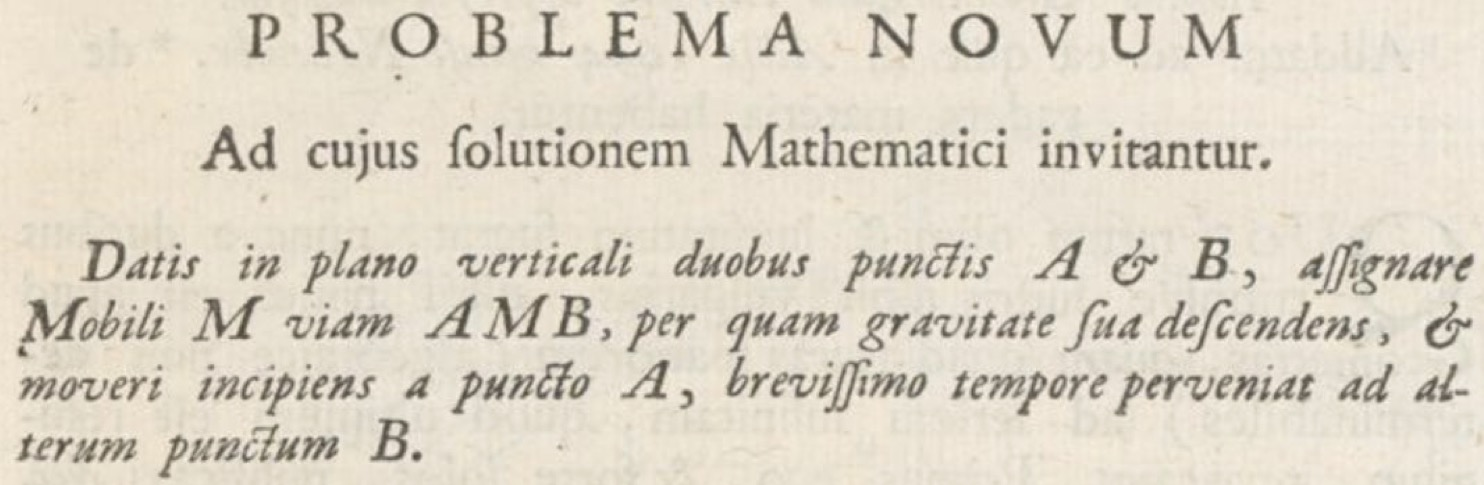
\includegraphics[width=0.8\textwidth]{chapters/020-variation/images/latein.jpg}
\end{center}
Zu deutsch:
\begin{quote}
Neue Aufgabe, zu deren Lösung die Mathematiker eingeladen werden.
Gegeben zwei Punkte $A$ und $B$ in einer vertikalen Ebene, finde
die Bahn $AMB$ eines Punktes $M$, der unter der Wirkung seines
Gewichtes in kürzester Zeit vom Punkt $A$ zum anderen Punkt $B$ absteigt.
\end{quote}
Die Situation der Aufgabenstellung ist in
Abbildung~\ref{buch:variation:fig:brachistochronenproblem}
dargestellt.
Bernoulli hat als Lösung gefunden, dass die Kurve eine Ausschnitt
aus einer Zykloide (in der Abbildung grau) sein muss.
Seine Lösung beruhte auf der Beobachtung, dass sich das Problem analog
zu einem Lichtausbreitungsproblem ist, für welches Fermat bereits
eine Lösung gefunden hat.

Da die Reibung vernachlässigt wird, ist die Energie des Massepunktes
erhalten.
Sie setzt sich aus der potenziellen und der kinetischen Energie
zusammen.
Die potenzielle Energie ist $-mgy$, die kinetische Energie ist
$\frac12mv^2$.
Die Energieerhaltung wird daher zu
\[
E=\frac12mv^2-mgy
\qquad\Rightarrow\qquad
v
=
\sqrt{2g}\!\sqrt{\frac{E}{gm}+y}
=
\!\sqrt{2(C+y)}.
\]
Durch Wahl einer anderen Zeiteinheit kann die Gleichung noch weiter
vereinfacht zu
\(
v = \sqrt{C+y}
\)
vereinfacht werden.
Gesucht ist also die zeitlich kürzeste Bahn eines Teilchens, 
dessen Geschwindigkeit auf bekannte Art $v(y)$ von der vertikalen
Koordinate abhängt.

%
% Das Fermat-Problem
%
\subsection{Das Fermat-Prinzip}
Bereits Fermat hat erkannt, dass das Brechnungsgesetz von Snellius
als Lösung eines Extremalproblems verstanden werden kann.

\begin{satz}[Fermat]
Sie $c/n_i$ die Geschwindigkeit, mit der sich Licht im Medium $M_i$
ausbreitet.
Ein Lichtstrahl von $A_1$ nach $A_2$ geht durch denjenigen Punkt $B$ 
auf der Grenzfläche zwischen den Medien, für den sich die Sinus der
Winkel $\alpha_i$ zwischen den Strahlen und der Normalen zur Grenzfläche
umgekehrt wie die $n_i$ verhalten, wenn also das Brechungsgesetz
\[
\frac{\sin\alpha_1}{\sin\alpha_2}
=
\frac{n_2}{n_1}
\]
gilt.
\end{satz}

\begin{proof}
Ohne der Beschränkung der Allgmeinheit können wir auf die Betrachtung
einer Ebene beschränken, die die beiden Punkte $A_i$ enthält und senkrecht
auf der Grenzfläche steht.
Wir dürfen weiter annehmen, dass die $x$-Achse in der Grenzfläche liegt 
und die Punkte $A_i$ die Koordinaten $(x_i,y_i)$ und der Punkt $B$ die
Koordinaten $(x,0)$ hat.
Es ist derjenige Punkt $x$ zu bestimmen, für den die Lichtzeit entlang 
des Pfades $A_1BA_2$ minimal wird.
Diese Zeit ist
\begin{align*}
t
&=
\frac{\overline{A_1B}}{c/n_1}
+
\frac{\overline{BA_2}}{c/n_2}
\\
ct
&=
n_1\overline{A_1B}
+
n_2\overline{A_2B}
\\
&=
n_1\!\sqrt{(x-x_1)^2 + y_1^2}
+
n_2\!\sqrt{(x_2-x)^2 + y_2^2}
\end{align*}
Das Minimum wird bei einer Nullstelle der Ableitung nach $x$ gefunden,
also bei einer Lösung der Gleichung
\begin{align*}
0
&=
n_1\frac{2(x_1-x)x}{\sqrt{(x_1-x)^2+y_1^2}}
+
n_2\frac{-2(x-x_2)x}{\sqrt{(x_2-x)^2+y_2^2}}.
\intertext{Indem man den zweiten Term auf der rechten Seite auf die linke
Seite bringt und durch $x$ dividiert, erhält man}
n_1
\frac{x_1-x}{\sqrt{(x_1-x)^2+y_1^2}}
&=
n_2
\frac{x-x_2}{\sqrt{(x_2-x)^2+y_2^2}}.
\end{align*}
Der Nenner ist auf beiden Seiten die Hypothenuse eines rechtwinkligen
Dreiecks, welches als Ankathete die Normale zur Grenzfläche hat.
Der Zähler ist die Gegenkathete des Winkels $\alpha_i$ zwischen der
Hypothenuse und der Normalen.
Daher ist der Quotient der Sinus des Winkels oder
\begin{equation}
n_1 \sin\alpha_1 = n_2 \sin\alpha_2.
\label{buch:variation:problem:eqn:snelliusinvariante}
\end{equation}
Die Gleichung~\eqref{buch:variation:problem:eqn:snelliusinvariante}
ist gleichbedeutend mit dem Brechungsgesetz
\[
\frac{\sin\alpha_1}{\sin\alpha_2}
=
\frac{n_2}{n_1}
\]
von Snellius.
\end{proof}

Der Satz von Fermat etabliert das Brechungsgsetz also Lösung eines
Extremalproblems.
Die Natur wählt für einen Lichtstrahl den zeitlich kürzesten Weg.
Der Beweis des Satzes von Fermat zeigt, dass entlang des Lichtstrahls
an jeder Grenzfläche zwischen Medien die Bedingung
\eqref{buch:variation:problem:eqn:snelliusinvariante}
erfüllt.
Wenn die optische Dichte $n$ eine Funktion von $n(y)$ ist, dann
wird der Lichtstrahl nicht nur in diskreten Punkten geknickt, sondern
entlang des ganzen Strahles gekrümmt.
Folgt der Strahl der Kurve $x(y)$, die mit der vertikalen den Winkel
$x'(y) = \tan\alpha(y)$ einschliesst.
Damit lässt sich auch die Sinus-Funktion ausdrücken, es gilt
\[
\sin\alpha(y)
=
\frac{x'(y)}{\pm\!\sqrt{x'(y)^2+1}}.
\]
Aus der Form~\eqref{buch:variation:problem:eqn:snelliusinvariante}
des Brechungsgesetztes wird dann die Gleichung
\begin{equation}
n_1\sin\alpha(y)
=
\frac{n_1(y)x'(y)}{\pm\!\sqrt{x'(y)^2+1}}
=
\operatorname{const}
\qquad\Rightarrow\qquad
\frac{n_1(y)^2x'(y)^2}{x'(y)^2+1}=C.
\label{buch:variation:eqn:fermatdgl}
\end{equation}
Dies ist eine Differentialgleichung für die Funktion $x(y)$.
Sie kann auch in die Form
\[
x'(y)^2
=
\frac{C}{(n_1(y)^2-C)}
\]
gebracht werden.

%
% Das Brachistochronenproblem als Lichtausbreitungsproblem
%
\subsubsection{Das Brachistochronenproblem als Lichtausbreitungsproblem}
Das Fermat-Prinzip besagt, dass ein Lichtstrahl, der sich in einem Medium
mit der Geschwindigkeit $c/n(y)$ ausbreitet, die Gleichung 
\eqref{buch:variation:eqn:fermatdgl} erfüllt.
Beim Brachistochronenproblem ist die Geschwindigkeit $v(y)=\!\sqrt{C-y}$ und 
damit $n(y) = c/\!\sqrt{C-y}$.
Eine Brachistochrone ist also eine Kurve, die die aus
\eqref{buch:variation:eqn:fermatdgl} folgende Gleichung
\begin{equation}
\frac{x'(y)^2}{(1+x'(y)^2)(C-y)} = K
\label{buch:variation:problem:eqn:bernoullidgl}
\end{equation}
erfüllen.

%
% Die Bernoullische Lösung
%
\subsubsection{Die Bernoullische Lösung}
Bernoulli hat gefunden, dass die Brachistochrone ein Zykloidenbogen ist.
Dies lässt sich dadurch verifizieren, dass man die Parametrisierung
einer Zykloide in die
Gleichung~\eqref{buch:variation:problem:eqn:bernoullidgl}
einsetzt.
Die Zykloide hat die Parametrisierung
\[
\left.
\begin{aligned}
x &= r(\varphi - \sin\varphi) 
\\
y &= r(1-\cos\varphi)
\end{aligned}
\right\}
\quad
\text{mit der Ableitung}
\quad
\left\{
\begin{aligned}
\dot{x}(\varphi) &= r(1-\cos\varphi)\\
\dot{y}(\varphi) &= r\sin\varphi
\end{aligned}
\right.
\]
für $\varphi\in\mathbb{R}$.
Die Ableitung ist
\[
x'(y)
=
\frac{\dot{x}(\varphi)}{\dot{y}(\varphi)}
=
\frac{1-\cos\varphi}{\sin\varphi}.
\]
Eingesetzt in \eqref{buch:variation:problem:eqn:bernoullidgl}
wird daraus
\[
\frac{\dot{x}(\varphi)^2}{
(\dot{y}(\varphi)^2 +\dot{x}(\varphi)^2)
(C-r(1-\cos\varphi))
}
=
\frac{(1-\cos\varphi)^2}{
((1-\cos\varphi)^2+\sin^2\varphi)
(C-r+r\cos\varphi)
}
=
K.
\]
Ausmultiplizieren im Nenner ergibt
\[
\frac{(1-\cos\varphi)^2}{
(1-2\cos\varphi+\cos^2\varphi+\sin^2\varphi)
(C-r+r\cos\varphi)
}
=
\frac{1-\cos\varphi}{
2(C-r+r\cos\varphi)
}
\]

%
% Das Brachistochronenproblem als Variationsproblem
%
\subsection{Das Brachistochronenproblem als Variationsproblem
\label{buch:variation:problem:subsection:variationsproblem}}
Die Bernoullische Lösung des Brachistochronenproblems verwendet die
Analogie zum Fermat-Prinzip.
Eine solche Analogie ist nur selten möglich, daher soll das Problem
jetzt in eine Form gebracht werden, in die auch viele ähnliche
Optimierungsproblem gebracht werden können.

Wir erinnern daran, dass die Geschwindigkeit des Massepunktes durch
$v(y)=\sqrt{C-y}$ gegeben ist.
Damit lässt sich die Zeit berechnen, die der Massepunkt entlang der
Lösungskurve braucht, wenn man diese als Funktion $y(x)$ mit beschreibt.
Die Punkte $A$ und $B$ sollen die $x$-Koordinaten $a$ bzw.~$b$ haben.
Für das Kurvenstück zwischen den $x$-Koordinaten $x$ und $x+\Delta x$
braucht der Massepunkt die Zeit
\[
\frac{ \sqrt{\Delta x^2 + \Delta y^2} }{v(y)}
=
\frac{ \sqrt{1 + y'(x)^2} }{ v(y) } \Delta x.
\]
Die Zeit ist das Integral
\begin{equation}
t
=
\int_a^b \frac{\sqrt{1+y'(x)^2}}{v(y(x))}\,dx
=
\int_a^b \sqrt{\frac{1+y'(x)^2}{C-y(x)}}\,dx.
\label{buch:variation:problem:eqn:brachint}
\end{equation}
Der Integrand auf der rechten Seite hängt nur von den Funktion $y(x)$
und $y'(x)$ ab.
Dies kommt vor allem daher, dass die Geschwindigkeit nur von $y$ abhängt,
nicht auch noch von $x$.
Im Allgemeinen wird man also davon ausgehen müssen, dass der Integrand
auch noch von $x$ abhängt.
Die Variationsrechnung befasst sich mit Problemen, in denen Funktionen
gefunden werden müssen, die ein Integral wie das in
\eqref{buch:variation:problem:eqn:brachint}
minimiert oder maximiert werden müssen.

\begin{definition}[Lagrange-Funktion des Brachistochronenproblems]
Die Lagrange-Funk\-tion des Brachistochronenproblems ist der
Integrand des Integrals
\eqref{buch:variation:problem:eqn:brachint},
\index{Lagrange-Funktion}%
also die Funktion
\[
L(x,y,y')
=
\sqrt{\frac{1+y^{\prime 2}}{C-y}}.
\]
\end{definition}

%
% Funktionale
%
\subsection{Funktionale
\label{buch:variation:problem:subsection:funktionale}}
Die Variationsrechnung löst Optimierungsproblem, die von einer
Funktion abhängen.
Um dies mathematisch präzis zu fassen, ist zunächst nötig, die Menge
der in Frage kommenden Funktionen so einzuschränken, dass die interessierende
Grösse überhaupt wohldefiniert ist.

%
% Vektorräume
%
\subsubsection{Vektorräume}
Zunächst sind die gemeinsamen algebraischen Eigenschaften zu charakterisieren,
die wir von den für unsere Untersuchungen zweckmässigen Funktionenmengen
erwarten.

\begin{definition}[Vektorraum]
Ein Vektorraum über den reellen Zahlen $\mathbb{R}$ ist einem Menge $V$ mit
zwei Operationen, der Addition und der Multiplikation mit Skalaren
\begin{align*}
    +\colon V\times V         &\to V : (u,v)\mapsto u+v
&
\cdot\colon \mathbb{R}\times V&\to V : (\lambda,v) \mapsto\lambda v
\end{align*}
mit den folgenden Eigenschaften.
\begin{enumerate}
\item
Es gelten die Assoziativgesetze
\begin{align*}
(u+v)+w&=u+(v+w)&&\text{für alle $u,v,w\in V$}\\
(\lambda \mu)v&=\lambda(\mu v)&&\text{für alle $\lambda,\mu\in\mathbb{R},\;v\in V$.}
\end{align*}
\item
Es gibt einen Vektor $0\in V$ mit der Eigenschaft $0+v=v$ für alle
Vektoren $v\in V$.
\item
Zu jedem Vektor $v\in V$ gibt es den entgegengesetzten Vektor $-v\in V$
mit der Eigenschaft, dass $-v+v=0$ ist.
\item
Die Addition von Vektoren ist kommutativ: $u+v=v+u$ für alle $u,v\in V$.
\item
Es gelten die Distributivgesetze 
\begin{align*}
(\lambda + \mu) v &= \lambda v + \mu v
	&\quad\text{für alle $\lambda,\mu\in\mathbb{R},\;v\in V$}\\
\lambda(u+v)      &= \lambda u + \lambda v
	&\quad\text{für alle $\lambda\in\mathbb{R},\;u,v\in V$}
\end{align*}
\end{enumerate}
\end{definition}

Die Mengen $\mathbb{R}^n$ erfüllen die genannten Eigenschaften, sind
also Vektorräume.
Die Definition eines Vektorraums ist aber viel allgemeiner, insbesondere
gehören dazu auch Mengen von Funktionen.
Damit wird es möglich, die Berechnungen in $\mathbb{R}^n$ auf Funktionen
auszudehnen.
Zum Beispiel bilden die stetigen Funktionen auf einem Intervall einen
Vektorraum, wie das folgende Beispiel zeigt.

\begin{beispiel}
Die Menge
\[
C([a,b])
=
\{f\colon[a,b]\to\mathbb{R}\mid \text{$f$ ist stetig}\}
\]
der stetigen Funktionen bildet einen Vektorraum.
Die Operationen sind die punktweise Addition von Funktionen und die
Multiplikation der Werte mit Skalaren, für $f,g\in C([a,b])$ und
$\lambda\in \mathbb{R}$ ist
\begin{align*}
(f+g)(x) &= f(x)+g(x)
&&\text{und}&
(\lambda f)(x) &= \lambda f(x).
\end{align*}
Entscheidend ist, dass die Addition von Funktionen und die Multiplikation
mit Skalaren nicht aus der Menge herausführt.
Tatsächlich wird in der Analysis gezeigt, dass die Summe stetiger Funktionen
wieder stetig ist und dass die Funktion $x\mapsto \lambda f(x)$ stetig,
wenn $f$ stetig ist.
Die übrigen Eigenschaften sind ebenfalls erfüllt, da sie bereits für die
Funktionswerte erfüllt sind.
\end{beispiel}

%
% Norm und Grenzwerte
%
\subsubsection{Norm und Grenzwerte}
Um Analysis zu betreiben, muss man ausdrücken können, dass eine Folge
von Funktionen konvergiert.
Dazu ist ein Abstandsbegriff zwischen Funktionen nötig.

\begin{definition}[Norm, normierter Raum]
Eine {\em Norm} auf einem Vektorraum $V$ ist eine Abbildung
\index{Norm}%
$\|\cdot\|\colon V\to\mathbb{R}^+_0$ mit nichtnegativen reellen Werten
und den folgenden Eigenschaften
\begin{itemize}
\item Definitheit: $\|v\|\ge 0$ für $v\in V$ mit Gleichheit 
genau dann, wenn $v=0$.
\index{Definitheit}%
\item Absolute Homogenität: Für alle Vektoren $v\in V$ und
\index{Homogenität}%
$\lambda\in\mathbb{R}$ gilt $\|\lambda v\| = |\lambda|\, \|v\|$.
\item Dreiecksungleichung: für alle Vektoren $u,v\in V$ gilt
\index{Dreiecksungleichung}%
$\|u+v\|\le \|u\|+\|v\|$.
\end{itemize}
Ein {\em normierter Raum} ist ein Vektorraum mit einer Norm.
\index{normierter Raum}%
\end{definition}

\begin{beispiel}
Der Vektorraum der stetigen Funktionen kann mit der Supremum-Norm
\[
\|f\| = \sup_{x\in[a,b]} |f(x)|
\]
zu einem normierten Raum gemacht werden.
Die Definitheit ist durch die Definition offensichtlich sichersgtellt.
Für $\|\lambda f\|$ finden wir
\[
\|\lambda f\|
=
\sup_{x\in[a,b]} |\lambda f(x)|
=
|\lambda|\,
\sup_{x\in[a,b]} |f(x)|
=
|\lambda|\, \|f\|,
\]
was die Homogenität zeigt.
Die Dreiecksungleichung folgt aus
\begin{align*}
\|f+g\|
&=
\sup_{x\in[a,b]} |f(x)+g(x)|
\\
&\le
\sup_{x\in[a,b]} (|f(x)|+|g(x)|)
\\
&\le
\sup_{x\in[a,b], y\in[a,b]} (|f(x)|+|g(y)|)
\\
&=
\sup_{x\in[a,b]} |f(x)|
+
\sup_{y\in[a,b]} |g(y)|
=
\|f\| + \|g\|.
\qedhere
\end{align*}
\end{beispiel}

Mit einer Norm ist es jetzt möglich, die Konvergenz von Folgen und den
Begriff des Grenzwertes zu definieren.

\begin{definition}[Cauchy-Folge, Grenzwert]
Eine Folge $(x_n)_{n\in\mathbb{N}}$ in $V$ in einem normierten Raum $V$
mit der Norm $\|\cdot\|$
heisst eine Cauchy-Folge, wenn es für jedes $\varepsilon>0$ eine
\index{Cauchy-Folge}%
$N\in \mathbb{N}$ gibt derart, dass
\[
\| x_n - x_m \| < \varepsilon
\quad\forall n,m\ge N.
\]
Der Vektor $x\in V$ heisst {\em Grenzwert} der Folge $(x_n)_{n\in\mathbb{N}}$,
\index{Grenzwert}%
wenn es zu jedem $\varepsilon > 0$ ein $N\mathbb{N}$ gibt derart, dass
\[
\|x_n-x\| < \varepsilon 
\quad\forall n\ge N.
\]
Die Folge $(x_n)_{n\in\mathbb{N}}$  in $V$ heisst {\em konvergent}, wenn
\index{konvergent}%
$x$ der Grenzwert von $(x_n)_{n\in\mathbb{N}}$ ist.
\end{definition}

Der durch die Supremum-Norm definierte Konvergenzbegriff ist die gleichmässige
Konvergenz.
Zur Erinnerung:
Eine Folge $f_n$ von Funktionen heisst gleichmässig konvergent gegen die
Funktion $f$, wenn es zu jedem
$\varepsilon >0$ ein $N\in\mathbb{N}$ gibt derart, dass
\[
|f_n(x) - f(x)|<\varepsilon\quad\forall n>N\text{ und }x\in [a,b].
\]
Die Supremum-Norm ist
\[
\|f_n(x) - f(x)\|
=
\sup_{x\in[a,b]} |f_n(x)-f(x)| < \varepsilon
\]
für alle $n>N$.
Dies ist genau die Konvergenz in der Norm $\|\cdot\|$.
Aus der Analysis ist bekannt, dass eine gleichmässig konvergente 
Funktionenfolge gegen eine stetige Funktion konvergiert.

\begin{definition}[Banach-Raum]
Ein normierter Raum $V$ heisst ein {\em Banach-Raum},
\index{Banach-Raum}%
wenn jede Cauchy-Folge in $V$ einen Grenzwert hat.
\end{definition}

\begin{beispiel}
Die Menge $C^1([0,2])$
der stetigen Funktionen auf dem Intervall $[0,2]$ ist ein normierter
Raum mit der Norm
\[
\|f\|_1
=
\int_0^2 |f(x)|\,dx,
\]
die auch die $L^1$-Norm heisst.
\index{L1-Norm@$L^1$-Norm}%
Zunächst ist nachzuprüfen, dass dies tatsächlich eine Norm ist.
Die Definitheit und die Homogenität von $\|\cdot\|_1$ ist klar, nur
die Dreiecksungleichung erfordert etwas Arbeit.
Für Funktionen $f,g\in L^1([0,2])$ gilt
\begin{align*}
\|f+g\|_1
&=
\int_0^2 |f(x)+g(x)|\,dx
\\
&\le 
\int_0^2 |f(x)|+|g(x)|\,dx
=
\int_0^2 |f(x)|\,dx
+
\int_0^2 |g(x)|\,dx
=
\|f\|_1+\|g\|_1,
\end{align*}
was die Dreeicksungleichung beweist.

Eine Cauchy-Folge in der $L^1$-Norm muss aber nicht unbedingt einen
stetigen Grenzwert haben.
Die Funktionen
\(
f_n(x) =
\begin{cases}
x^n&\quad x< 1\\
1&\quad x\ge 1
\end{cases}
\)
haben die $L^1$-Norm
\begin{align*}
\|f_n-f_m\|_1
=
\int_0^2 |f_n(x)-f_m|\,dx
\\
&=
\biggl|\int_0^1 x^n-x^m\,dx\biggr|
=
\biggl[
\biggl|
\frac{1}{n+1}x^{n+1}
-
\frac{1}{m+1}x^{m+1}
\biggr|
\biggr]_0^1
\\
&=
\biggl|
\frac{1}{n+1}
-
\frac{1}{m+1}\biggr|.
\end{align*}
Wegen
\[
\|f_n-f_m\|_1
<\varepsilon
\]
für $n,m>2/\varepsilon$ ist $f_n$ eine Cauchy-Folge in $L^1$.
In $L^1$ konvergiert die Folge $f_n$ gegen die Funktion
\[
f(x)
=
\begin{cases}
0&\quad x< 1\\
1&\quad x\ge 1.
\end{cases}
\]
Diese Funktion ist aber nicht stetig, da sie bei $x=1$ einen
Sprung hat.
Bezüglich der $L^1$-Norm ist $C^1([a,b])$ als im Allgemeinen
kein Banach-Raum.
\end{beispiel}

%
% Stetige und differenzierbare Funktionen
%
\subsubsection{Stetige und differenzierbare Funktionen}
Mit der Norm lässt sich auch die Stetigkeit von Abbildungen zwischen
normierten Räumen definieren.

\begin{definition}[Stetigkeit]
Eine Funktion $f\colon U\to V$ zwischen normierten Räumen heisst
{\em stetig im Punkt} $x\in U$, wenn es zu jedem $\varepsilon > 0$
\index{stetig in einem Punkt}%
ein $\delta > 0$
gibt derart, dass
\(
\|f(x)-f(y)\| < \delta
\)
wenn
\(
\|x-y\|<\varepsilon
\).
Eine Funktion $f\colon U\to V$ heisst {\em stetig}, wenn sie in
jedem Punkt von $U$ stetig ist.
\end{definition}

Das Bild einer Folge $x_n\in U$, die gegen $x_0\in U$ konvergiert,
ist eine Folge $f(x_n)$ in $V$.
Man sagt, $y\in V$ sei der Grenzwert von $f(x)$ für $x\to x_0$,
wenn $f(x_n)$ für jede solche Folge $x_n$ gegen $y$ konvergiert.
Der Grenzwert wird auch
\[
\lim_{x\to x_0} f(x)
=
y
\]
geschrieben.
Stetige Funktionen zeichnen sich wie in der Analysis der Funktionen
einer Variablen dadurch aus, dass der Grenzwert der Werte der Funktion
auf einer konvergenten Folge mit dem Funktionswert des Grenzwertes
übereinstimmt.

\begin{satz}
Eine Funktion $f\colon U\to V$ ist genau dann stetig im Punkt $x\in U$,
wenn für jede Folge $x_n$ in $U$ mit Grenzwert $x$ die Folge $f(x_n)$
konvergent ist und
\[
\lim_{n\to\infty} f(x_n) = f(x).
\]
Eine lineare Funktion $f\colon U\to V$ ist genau dann stetig,
wenn für jede Nullfolge $x_n$ in $U$ 
\[
\lim_{n\to \infty} f(x_n) = 0
\]
gilt.
\end{satz}

\begin{definition}
Eine Funktion $f\colon U\to V$ zwischen normierten Räumen heisst
differenzierbar im Punkt $x\in U$ wenn es eine lineare Funktion
$Df(x_0)\colon U\to V$ gibt derart, dass
\[
f(x+v) =f(x) + Df(x_0)\cdot v + o(v),
\]
wobei $o(v)$ bedeutet, dass für diese Funktion
\[
\frac{o(v)}{|v|}\to 0
\quad\text{für $v\to 0$}
\]
gilt.
\end{definition}

Funktionen auf einem Vektorraum mit reellen Werten weren auch
{\em Funktionale} genannt.
\index{Funktional}
Vor dem 20.~Jahrhundert wurde häufig ein Untersschied zwischen
Funktionen von endlich vielen reellen Variablen und Funktionen
von einem unendlichdimensionalen Vektorraum gemacht.
Die Entwicklungen dieses  Abschnittes haben gezeigt, dass eine
solche Unterscheidung nicht gerechtfertigt ist.
Es ist lediglich notwendig, die Definitionen allgemein genug zu
fassen und sich jederzeit über die Funktionenmenge und die zu
verwendende Norm Rechenschaft abzulegen.


%
% 2-fundamtenallemma.tex
%
% (c) 2023 Prof Dr Andreas Müller
%
\section{Das Fundamentallemma
\label{buch:variation:section:fundamentallemma}}
\kopfrechts{Das Fundamentallemma}
Im Fall des endlichdimensionalen Extremalproblems ist aus der
Forderung, dass alle Richtungsableitung verschwinden müssen, 
die Bedingung geworden, dass
\[
v\cdot\grad f = 0
\]
sein muss für alle Vektoren $v\in\mathbb{R}^n$.
Wir haben daraus geschlossen, dass der Gradient $\grad f=0$
sein muss.
Wir hatten dies das endlichdimensionale Fundamentallemma genannt,
wegen $e_k\cdot \grad f = D_kf$ war es eine ziemliche Selbstverständlichkeit.
Bei der Lösung von Variationsproblemen, wo es nicht um endlichdimensionale
Vektoren und das Skalarprodukt, sondern um Funktionen und Integrale
geht, brauchen wir eine ähnliche Aussage für Funktionen.

%
% Positive glatte Funktionen mit kompaktem Träger
%
\subsection{Positive glatte Funktionen mit kompaktem Träger}
Die Aussage des Fundamentallemmas für endlichdimensionale Vektoren 
folgte sofort aus der Tatsache, dass es für jedes $k$ einen Vektor
$e_k$ gibt, der nur in der Koordinaten $k$ von $0$ verschieden ist.
Natürlich gibt es auch Funktionen, die nur in genau einem Punkt
von $0$ verschieden sind.
Eine solche Funktion ist aber im allgemeinen nicht differenzier-
oder integrierbar.
In diesem Abschnitt soll daher gezeigt werden, dass es unendlich
oft stetig differnzierbare Funktionen gibt, die nur in einem beliebig
kleinen vorgegebenen Intervall $\ge 0$ sind.

\begin{definition}[Träger]
Der {\em Träger} einer Funktion $f\colon X\to\mathbb{R}$ ist die Menge
\index{Träger}%
\[
\supp f = \{ x\in X\mid f(x)\ne \}.
\]
\end{definition}

Gesucht ist also eine beliebig oft stetig differenzierbare Funktion,
deren Träger in einem vorgegebenen Intervall $[a,b]$ enthalten ist.
Wir konstruieren so eine Funktion in zwei Schritten.

\input{chapters/020-variation/fig/f.tex}

\begin{satz}
\label{buch:variation:fundamentallemma:satz:glatt}
Die Funktion
\[
f(x)
=
\begin{cases}
e^{-1/x}&\qquad x>0\\
0&\qquad x\le 0
\end{cases}
\]
(siehe auch Abbildung~\ref{buch:variation:fundamentallemma:fig:glatt})
ist beliebig oft stetig differenzierbar.
\end{satz}

\begin{proof}
Es ist klar, dass die Funktion $f$ beliebig oft stetig differenzierbar
ist in jedem Punkt $x\ne 0$.
Es ist also nur nachzuweisen, dass $f(x)$ im Punkt $0$ beliebig
oft stetig differenzierbar ist.

Die ersten drei Ableitungen von $f(x)$ sind
\begin{align}
f'(x) &= \frac{1}{x^2} f(x)
\label{buch:variation:fundamentallemma:eqn:f1}
\\
f''(x) &= \frac{1-2x}{x^4}f(x)
\notag
\\
f'''(x) &= \frac{6x^2-6x+1}{x^6}f(x).
\notag
\end{align}
Daraus lässt sich die Vermutung ableiten, dass
\begin{equation}
f^{(n)}(x)
=
\frac{p_{n-1}(x)}{x^{2n}} f(x)
\label{buch:variation:fundamentallemma:eqn:fabl}
\end{equation}
ist, wobei $p_k(x)$ ein Polynom vom Grad $k$ ist.
Wir beweisen diese Vermutung mit Hilfe von vollständiger Induktion.
Die Induktionsverankerung für die $0$-te Ableitung ist trivial.

Wir nehmen jetzt im Sinne der Induktionsannahme an, dass die $n$-te
Ableitung die Form \eqref{buch:variation:fundamentallemma:eqn:fabl}
hat.
Wir müssen zeigen, dass dann auch $f^{(n+1)}(x)$ diese Form hat.
Dazu berechnen wir
\begin{align}
f^{(n+1)}(x)
&=
\frac{d}{dx}
\frac{p_n(x)}{x^{2n}} f(x)
\notag
\\
&=
\frac{p_n'(x)}{x^{2n}} f(x)
-2n
\frac{p_n(x)}{x^{2n+1}} f(x)
+
\frac{p_n(x)}{x^{2n}} f'(x).
\notag
\intertext{Mit der ersten Ableitung
\eqref{buch:variation:fundamentallemma:eqn:f1} wird dies zu}
&=
\frac{p_n'(x)}{x^{2n}} f(x)
-2n
\frac{p_n(x)}{x^{2n+1}} f(x)
+
\frac{p_n(x)}{x^{2n}} \frac{1}{x^2}f(x)
\notag
\\
&=
\frac{x^2p_n'(x) -2nxp_n(x)+p_n(x)}{x^{2n+2}} f(x).
\label{buch:variation:fundamentallemma:eqn:induktionsschritt}
\end{align}
Die Ableitung $p_n'(x)$ ist ein Polynom vom Grad $n-1$ und damit
ist $x^2p_n'(x)$ ein Polynom vom Grad $n+1$.
Ebenso ist $xp_n(x)$ ein Polynom vom Grad $n+1$ während
$p_n(x)$ ein Polynom vom Grad $n$ ist.
Der Zähler von
\eqref{buch:variation:fundamentallemma:eqn:induktionsschritt}
ist
\[
p_{n+1}(x)
=
x^2p_n'(x)+(1 -2nx)p_n(x),
\]
ein Polynom vom Grad $n+1$.
Damit ist der Induktionsschritt erfolgreich und die Behauptung betreffend
die Form von $f^{(n)}(x)$ ist bewiesen.

Es ist jetzt nur noch zu zeigen, dass der Grenzwert von $f^{(n)}(x)$
für $x\to 0+$ verschwindet.
Da das Polynom $p_n(x)$ stetig ist, folgt
\[
\lim_{x\to 0}
f^{(n)}(x)
=
\lim_{x\to 0}\frac{p_n(x)}{x^{2n}}f(x)
=
p_n(0) \lim_{t\to\infty} t^{2n} e^{-t}
=
0.
\]
Damit ist die beliebige stetige Differenzierbarkeit an der Stelle
$x=0$ gezeigt.
\end{proof}

Die Funktion $f(x)$ von 
Satz~\ref{buch:variation:fundamentallemma:satz:glatt} 
erfüllt noch nicht die Forderung, dass sie nur in einem vorgegebenen
Intervall von $0$ verschieden ist.

\input{chapters/020-variation/fig/g.tex}

\begin{satz}
\label{buch:variation:fundamentallemma:satz:gab}
Sei $f(x)$ die Funktion von
Satz~\ref{buch:variation:fundamentallemma:satz:glatt}.
Dann ist
\[
g_{a,b}(x)
=
f(x-a) f(b-x)
\]
eine unendlich oft stetig differenzierbare, nichtnegative Funktion mit Träger
$\supp g_{a,b}=(a,b)$.
\end{satz}

Die Funktionen $g_{a,b}(x)$ sind beliebig oft differenzierbar und nur im
Intervall $[a,b]$ von $0$ verschieden und sogar positiv.
Weil sie stetig sind, sind sie auch integrierbar, man kann also das
Integral über $\mathbb{R}$ berechnen und die Funktion damit normieren.
Die neue Funktion
\[
\frac{1}{N}
\tilde{g}_{a,b}(x)
\qquad\text{mit}\;
N
=
\int_{-\infty}^{\infty}g_{a,b}(x)\,dx
=
\int_a^b g_{a,b}(x)\,dx
\]
ist immer noch beliebig oft stetig differenzierbar und hat zusätzlich die
Eigenschaft
\[
\int_{-\infty}^{\infty}
\tilde{g}_{a,b}(x)\,dx
=
\int_a^b
\tilde{g}_{a,b}(x)\,dx
=
1.
\]
Wir formulieren dieses Resultat als Satz.

\begin{satz}
\label{buch:variation:satz:gabeins}
Zu jedem Intervall $[a,b]$ gibt es eine beliebig oft stetig
differenzierbare Funktion $g(x)$, genau das Intervall $[a,b]$
als Träger hat und deren Integral über $[a,b]$ den Wert $1$ hat.
\end{satz}

%
% Das Fundamentallemma
%
\subsection{Das Fundamentallemma}
Mit der Funktion $g_{a,b}(x)$ von
Satz~\ref{buch:variation:fundamentallemma:satz:gab}
lässt sich jetzt das Fundamentallemma in der folgenden Form
leicht beweisen.

\begin{satz}[Fundamentallemma]
\label{buch:variation:fundamentallemma:satz:fundamentallemma}
Wenn für die stetige Funktion $f\colon[a,b]\to\mathbb{R}$ 
\begin{equation}
\int_a^b f(x)\varphi(x)\,dx = 0
\label{buch:variation:fundamentallemma:eqn:fundamentalbed}
\end{equation}
gilt für jede beliebig oft stetig differenzierbare Funktion $\varphi(x)$ 
dann ist $f(x)=0$.
Das Resultat gilt selbst dann, wenn
\eqref{buch:variation:fundamentallemma:eqn:fundamentalbed}
nur für beliebig oft stetig differenzierbare Funktionen $\varphi(x)$ 
gilt, die ausserdem an den Intervallenden verschwinden:
$\varphi(a)=\varphi(b)=0$.
\end{satz}

\begin{proof}
Wir zeigen mit Hilfe eines Widerspruchs, dass es keinen Punkt $x_0\in[a,b]$
geben kann, für den $f(x_0)\ne 0$ ist.
Dazu nehmen wir also an, dass $f(x_0)\ne 0$ ist.
Falls $f(x_0)<0$ ist, ersetzen wir $f$ durch $-f$, 
die Bedingung
\eqref{buch:variation:fundamentallemma:eqn:fundamentalbed}
ändert sich dadurch nicht.
\input{chapters/020-variation/fig/fundamentallemma.tex}
Wir dürfen daher annehmen, dass $f(x_0)>0$ ist
(Abbildung~\ref{buch:variation:fundamentallemma:fig:beweis}).
Da $f$ stetig ist, gibt es ein Intervall $[x_0-\varepsilon,x_0+\varepsilon]$
derart, dass $f(x)> \frac12 f(x_0)$ für
$x\in[x_0-\varepsilon,x_0+\varepsilon]$ gilt.
Dann gilt für das Integral
\[
\int_a^b
f(x)
g_{x_0-\varepsilon,x_0+\varepsilon} (x)
\,dx
>
\frac{f(x_0)}{2}
\int_a^b
g_{x_0-\varepsilon,x_0+\varepsilon} (x)
\,dx
>
0
\]
im Widerspruch zur Bedingung
\eqref{buch:variation:fundamentallemma:eqn:fundamentalbed}.
Der Widerspruch zeigt, dass $f(x)=0$ sein muss.
\end{proof}

%
% Skalarproduktformulierung des Fundamentallemmas
%
\subsection{Skalaproduktformulierung des Fundamentallemmas}
Die Richtungsableitung einer Funktion endlich vieler Variablen 
konnte als Skalarprodukt mit dem Gradienten geschrieben werden und
das Fundamentallemma hat besagt, dass der Gradient verschwindet,
wenn alle Richtungsableitungen verschwinden.
Diese Schlussweise ist auch für Funktionen möglich, wenn man Funktionen
ein Skalarprodukt definieren kann.

\begin{definition}[$L^2$-Skalarprodukt]
Das {\em Skalarprodukt} zweier quadratintegrierbarer Funktion $f$ und $g$
auf dem Intervall $[a,b]$ ist definiert durch
\[
\langle f,g\rangle
=
\int_a^b f(x)g(x)\,dx.
\]
\end{definition}

\begin{satz}[Fundamentallemma, Skalarproduktform]
Wenn für eine stetige Funktion $f\colon[a,b]\to\mathbb{R}$ das Skalarprodukt
\[
\langle f,\varphi\rangle = 0
\]
ist für jede unendlich oft differenzierbare Funktion $\varphi$ auf dem
Intervall $[a,b]$, dann ist $f=0$.
\end{satz}



%
% 3-eulerlagrange.tex
%
% (c) 2023 Prof Dr Andreas Müller
%
\section{Die Euler-Lagrange Differentialgleichung
\label{buch:variation:section:eulerlagrange}}
\kopfrechts{Die Euler-Lagrange Differentialgleichung}
Das Neuartige an der Aufgabenstellung des Brachistochronenproblems
war, dass eine Funktion gesucht war, so dass ein damit gebildetes
Integral eine Minimaleigenschaft erfüllt.
Für die damalige Mathematik war die Aufgabe, eine Funktion zu finden,
nicht neu.
Die Theorie der Differentialgleichungen war bereits entwickelt,
Newton hat die Infinitesimalrechnung ja erfunden, um damit die
Bewegungsgleichungen der Physik zu formulieren und zu lösen.
In einer Differentialgleichung werden Werte und Ableitungen einer
Funktion an einer einzigen Stelle miteinander verbunden.
Etwas salop formuliert sagt die Differentialgleichung in jedem
Punkt, in welche Richtung und mit welcher Krümmung die Funktionskurve
weiter zu zeichnen ist.

Im Brachistochronenproblem tragen aber alle Werte der gesuchten
Funktion zum Integral bei, es scheint daher auf den ersten Blick
nicht möglich, das Problem durch schrittweise Konstruktion
``von Punkt zu Punkt'' der Lösungskurve zu konstruieren.

Bernoullis Lösung des Brachistochrononproblems beruht auf der
Beobachtung, dass sich die Bedinung für die schnellste Bahn
durch eine Bedingung ersetzen lässt, die in jedem einzelnen
Punkt ausgewertet werden kann.
Das von ihm verwendete Fermat-Prinzip wurde ursprünglich ebenfalls
als eine globale Eigenschaft eines Lichtstrahls formuliert.
Aus dem Fermat-Prinzip folgt aber das Brechungsgesetz, welches
sagt, dass die Richtung eines Strahls in einem Punkt genau dann
ändert, wenn sich dort auch der Brechungsindex der beiden Medien
ändert.
Das Fermat-Prinzip ist also ein Beispiel dafür, wie eine globale
Bedingung erfüllt werden kann, indem einer lokalen Regel in jedem
Punkt gefolgt wird.

Es ist das Verdienst von Euler und Lagrange, zu erkennen, dass diese
Übersetzung eines globalen Variationsproblems in ein lokales 
Problem immer möglich ist.
Es entsteht dabei die Euler-Lagrange-Differentialgleichung, welche
die Problemstellung auf die Lösung einer Differentialgleichung
reduziert.
Damit ist ein allgemein anwendbares Lösungsverfahren gefunden.
Zu einem Variationsproblem lässt sich immer eine Differentialgleichung
finden, welche die gesuchte Funktion als Lösung hat.

In diesem Abschnitt soll dieser indirekte Weg der Lösung von
Variationsaufgaben dargestellt werden.
Wir werden später zeigen, dass diese Vorgehensweise nicht immer
erfolgreich sein kann.
Zum Beispiel werden wir in Kapitel~\ref{buch:chapter:nichtdiff}
Variationsprobleme kennenlernen, deren Lösungskurven nicht
differenzierbar sind und daher auch nicht von einer Differentialgleichung
gefunden werden können.
Im Kapitel~\ref{buch:chapter:direkt} werden daher die sogenannten
direkten Methodn vorgestellt, die den Umweg über eine
Differentialgleichung vermeiden.

%
% Die Lagrange-Funktion
%
\subsection{Die Lagrange-Funktion
\label{buch:variation:eulerlagrange:subsection:lagrange-funktion}}
Wir betrachten Variationsproblem der folgenden Art.
Gesucht ist eine auf dem Intervall $[x_0,x_1]$ definirte
Funktion $y(x)$, die das Integral
\begin{equation}
I(y)
=
\int_{x_0}^{x_1}
F(x, y(x), y'(x))
\,dx
\label{buch:variation:eulerlagrange:eqn:funktional}
\end{equation}
maximiert oder minimiert.
Der Ausdruck~\eqref{buch:variation:eulerlagrange:eqn:funktional}
wird ein Funktional genannt.
Die Funktion
\[
F
\colon
\mathbb{R}\times
\mathbb{R}\times
\mathbb{R}
\to
\mathbb{R}
\]
von drei Variablen heisst die {\em Lagrange-Funktion}
des Funktionals \eqref{buch:variation:eulerlagrange:eqn:funktional}.

\begin{beispiel}
Die Lagrange-Funktion des Brachistochronenproblems ist
\[
F(x,y,y')
=
\sqrt{ \frac{1+y^{\prime 2}}{y} }.
\]
Die Funktion hängt nicht von $x$ ab, was bedeutet, dass eine
Verschiebung in $x$-Richtung die Form der Lösungsfunktion des
Variationsproblems nicht ändert.
\end{beispiel}

\begin{beispiel}
\label{buch:variation:eulerlagrange:beispiel:gerade}
Wir formulieren die Aufgabe, die kürzeste Verbindung der Punkte
$(x_0,y_0)$ und $(x_1,y_1)$ in einer Ebene zu finden, als Variationsproblem.
Die Länge einer Kurve $y(x)$ ist das Integral
\[
l(y)
=
\int_{x_0}^{x_1}
\sqrt{1+y'(x)^2}\,dx.
\]
Daraus lesen wir ab, dass die Lagrange-Funktion dieses Variationsproblems
\begin{equation}
F(x,y,y') = \sqrt{1+y^{\prime 2}}
\label{buch:variation:eulerlagrange:eqn:geradeL}
\end{equation}
ist.
Die Funktion hängt weder von $x$ noch von $y$ ab.
Dies ist auch zu erwarten, denn die Länge einer Kurve hängt nicht davon
ob, wo in der Ebene sie platziert ist.
Eine Verschiebung in $x$-Richtung würde das $x$-Argument ändern,
eine Verschiebung in $y$-Richtung die $y$-Werte.
Wäre $F$ von $x$ oder $y$ abhängig, könnte auch die Länge der Kurve
davon abhängen.
\end{beispiel}

%
% Euler-Lagrange_Differentialgleichung
%
\subsection{Euler-Lagrange-Differentialgleichung
\label{buch:variation:eulerlagrange:subsection:dgl}}
\input{chapters/020-variation/fig/variation0.tex}
Das Maximum oder Minimum einer Funktionen mehrere Variablen wurde
gefunden, indem die Richtungsableitung berechnet und $=0$ gesetzt
wurde.
Um die Funktion zu bestimmen, die ein Funktional $I(y)$ zu einem
Maximum oder Minimum macht, versuchen wir, die Idee der Richtungsableitung
für ein Funktional nachzuahmen.
Wir nehmen daher an, dass $y(x)$ eine Funktion ist, die das Funktional
$I(y)$ zu einem Minimum macht.
Für die Richtungsableitung addieren wir ein Vielfaches einer
Funktion $\eta(x)$, die Summe $y(x)+\varepsilon\eta(x)$ entspricht
dann einer Geraden mit Richtung $\eta(x)$ im Funktionenraum
(Abbildung~\ref{buch:variation:fig:variation0}).
Die Funktionen $y(x)+\varepsilon\eta(x)$ sind aber nur dann Kandidaten
für eine Lösung des Problems, wenn immer noch
\begin{align*}
y(x_0) + \varepsilon \eta(x_0) &= y_0
&&\text{und}&
y(x_1) + \varepsilon \eta(x_1) &= y_1
\end{align*}
gilt.
Dies ist nur möglich, wenn $\eta(x_0)=\eta(x_1)=0$ ist.

Wir berechnen jetzt die Ableitung der Funktion
$\varepsilon\mapsto I(y+\varepsilon\eta )$ an der Stelle $\varepsilon=0$.
Da die Intervallgrenzen nicht von $\varepsilon$ abhängen, können wir
die Ableitung unter das Integral nehmen:
\begin{align*}
\frac{d}{d\varepsilon}
I(y+\varepsilon\eta)
&=
\int_{x_0}^{x_1}
\frac{d}{d\varepsilon}
F(x,y(x)+\varepsilon\eta(x),y(x)+\varepsilon\eta'(x))
\,dx.
\intertext{Da $F$ differenzierbar ist, kann die Ableitung mit der
Kettenregel berechnet werden, sie ist}
&=
\int_{x_0}^{x_1}
\frac{\partial F}{\partial y}
(x,y(x)+\varepsilon\eta(x),y(x)+\varepsilon\eta'(x))
\eta(x)
\\
&\qquad
+
\frac{\partial F}{\partial y'}
(x,y(x)+\varepsilon\eta(x),y(x)+\varepsilon\eta'(x))
\eta'(x)
\,dx.
\intertext{Uns interessiert aber nur der Wert an der Stelle $\varepsilon=0$,
er ist}
\frac{d}{d\varepsilon}
I(y+\varepsilon\eta)
\bigg|_{\varepsilon=0}
&=
\int_{x_0}^{x_1}
\frac{\partial F}{\partial y}
(x,y(x),y'(x))
\,
\eta(x)
+
\frac{\partial F}{\partial y'}
(x,y(x),y'(x))
\,
\eta'(x)
\,dx
=0.
\end{align*}
Das Integral hängt von den verschiedenen Faktoren $\eta(x)$ und
von $\eta'(x)$ in den beiden Termen unter dem Integral ab.
Wir integrieren den zweiten Term partiell 
\begin{align*}
\int_{x_0}^{x_1}
\frac{\partial F}{\partial y'}(x,y(x),y'(x))\,\eta'(x)\,dx
&=
\biggl[
\frac{\partial F}{\partial y'}(x,y(x),y'(x))\,\eta(x)
\biggr]_{x_0}^{x_1}
\\
&\qquad
-
\int_{x_0}^{x_1}
\frac{d}{dx}
\frac{\partial F}{\partial y'}(x,y(x),y'(x))\,\eta(x)\,dx.
\end{align*}
Da $\eta(x_0)=\eta(x_1)=0$ verschwindet der erste Term
auf der rechten Seite, es bleibt
\[
\frac{d}{d\varepsilon}
I(y+\varepsilon\eta)
\bigg|_{\varepsilon=0}
=
\int_{x_0}^{x_1}
\biggl(
\frac{\partial F}{\partial y}
(x,y(x),y'(x))
-
\frac{d}{dx}
\frac{\partial F}{\partial y'}
(x,y(x),y'(x))
\biggr)
\eta(x)
\,dx.
\]
Dies kann auch als Skalarprodukt
\[
\biggl\langle 
\frac{\partial F}{\partial y}
(x,y(x),y'(x))
-
\frac{d}{dx}
\frac{\partial F}{\partial y'}
(x,y(x),y'(x))
,
\eta(x)
\biggr\rangle
=
0
\]
geschrieben werden.
Da dies für jede differenzierbare Funktion $\eta$ mit Randwerten
$\eta(x_0)=\eta(x_1)$ gelten muss, folgt nach dem
Fundamentallemma~\ref{buch:variation:fundamentallemma:satz:fundamentallemma},
der folgende Satz. 

\begin{satz}[Euler-Lagrange]
\label{buch:variation:eulerlagrange:satz:eulerlagrange}
Wenn die mindestens zweimal stetig differenzierbare Funktion $y(x)$
unter allen solchen Funktionen mit $y(x_0)=y_0$ und $y(x_1)=y_1$
das Funktional
\[
I(y)
=
\int_{x_0}^{x_1}
F(x,y(x),y'(x))\,dx
\]
zu einem Maximum oder Minimum macht, dann ist $y(x)$ eine Lösung der
gewöhnlichen Differentialgleichung
\begin{equation}
\frac{d}{dx}
\frac{\partial F}{\partial y'}(x,y(x),y'(x))
-
\frac{\partial F}{\partial y}(x,y(x),y'(x))
=
0.
\label{buch:variation:eulerlagrange:eqn:eulerlagrange}
\end{equation}
Sie heisst die {\em Euler-Lagrange-Differentialgleichung}.
\end{satz}

Eine Lösung des Variationsproblems kann also als Lösung der
Euler-Lagrange-Dif\-fe\-ren\-tial\-glei\-chung mit den Randwerten
$y(x_0)=x_0$ und $y(x_1)=y_1$ gefunden werden.
Die Bedingung ist notwendig, aber nicht hinreichend.
Wie bei der Bestimmung eines Extremums bei Funktionen endlich
vieler Variablen garantiert das Verschwinden der Richtungsableitung
nicht, dass auch tatsächlich ein Extremum vorliegt.
Man sagt daher auch, dass eine Lösung $y(x)$ der
Euler-Lagrange-Differentialgleichung das Funktional $I(y)$
stationär macht.

Eine weitere Einschränkung ist, dass die Herleitung der
Euler-Lagrange-Differential\-gleichung vorausgesetzt hat,
dass die Lösungsfunktion $y(x)$ mindestens zweimal 
stetig differenzierbar ist.
Es gibt aber durchaus Variationsprobleme, deren Lösungen
nicht differenzierbar sind, dazu mehr im Kapitel~\ref{buch:chapter:nichtdiff}.

\begin{beispiel}
\label{buch:variation:eulerlagrange:beispiel:gerade}
Wir lösen das Variationsproblem von Beispiel
\ref{buch:variation:eulerlagrange:beispiel:gerade}
mit der Lagrange-Funk\-tion
\eqref{buch:variation:eulerlagrange:eqn:geradeL}.
Da die Lagrange-Funktion nicht von $y$ abhängt, bleibt von der 
Euler-Lagrange-Gleichung nur
\[
\frac{d}{dx}
\frac{\partial L}{\partial y'}(x,y(x),y'(x))
=
0
\]
übrig.
Berechnung der Ableitung liefert
\begin{equation}
\frac{\partial}{\partial y'}
\sqrt{1+y^{\prime 2}}
=
\frac{y'}{\sqrt{1+y^{\prime 2}}}.
\label{buch:variation:eulerlagrange:eqn:ableitungFyp}
\end{equation}
Die Ableitung nach $x$ ergibt
\begin{align*}
\frac{d}{dx}
\frac{\partial}{\partial y'}
\sqrt{1+y^{\prime 2}}
&=
\frac{d}{dx}
\frac{y'}{\sqrt{1+y^{\prime 2}}}
\\
&=
\frac{
y''\sqrt{1+y^{\prime 2}}-y'\cdot \frac{y'y''}{\sqrt{1+y^{\prime 2}}}
}{
1+y^{\prime 2}
}
\\
&=
y''
\frac{
1+y^{\prime 2}-y^{\prime 2}
}{
(1+y^{\prime 2})^{\frac32}
}.
\intertext{Die Euler-Lagrange-Differentialgleichung ist daher}
0
&=
\frac{y''}{(1+y^{\prime 2})^{\frac32}} .
\end{align*}
Der Nenner auf der rechten Seite ist immer $\ge 1$, die Gleichung kann
also nur erfüllt sein, wenn $y''=0$ ist.
Die Funktion $y(x)$ muss also eine lineare Funktion $y=ax+b$ sein.
Die Randbedingung wird erfüllt für die Geradengleichung
\[
y(x)
=
\frac{y_1-y_0}{x_1-x_0}(x-x_0) + y_0.
\]
Kürzeste Verbindungen in der Ebene sind daher Geraden.
\end{beispiel}

%
% Freie Randbedingungen
%
\subsection{Freie Randbedingungen
\label{buch:variation:eulerlagrange:subsection:freierb}}
In der Herleitung der Euler-Lagrange-Differentialgleichung wurde angenommen,
dass die Endpunkte der Lösungsfunktion durch $y(x_0)=y_0$ und $y(x_1)=y_1$
fest vorgegeben sind.
Diese Voraussetzung soll in diesem Abschnitt abgeschwächt werden.
Die Funktionswerte in den Endpunkten sollen also nicht mehr fest
vorgegeben sein.

\begin{beispiel}
\label{buch:variation:eulerlagrange:beispiel:freiegerade}
Im Beispiel~\ref{buch:variation:eulerlagrange:beispiel:gerade}
wurde die kürzeste Kurve zwischen zwei Punkten in der Ebene
gesucht und wie erwartet eine Gerade als Lösung gefunden.
Wenn die Werte $y_0$ und $y_1$ jetzt nicht mehr vorgegeben sind,
wird die kürzeste Verbindung zwischen den beiden Geraden
$x=x_0$ und $x=x_1$ gesucht.
Die Lösung dieses Problems ist nicht eindeutig, jede horizontale
Strecke mit $y_0=y_1$ ist eine Lösung.
\end{beispiel}

Das Beispiel zeigt, dass es im Allgemeinen immer noch die Vorgabe
eines der beiden Randwerte braucht, um die Lösung eindeutig zu
bestimmen.
Wir lösen daher die folgende Aufgabe.

\begin{aufgabe}
Gesucht ist eine zweimal stetig differnzierbare Funktion $y(x)$ auf
dem Intervall $[x_0,x_1]$ mit $y(x_0)=y_0$, die das Integral
\[
I(y)
=
\int_{x_0}^{x_1} F(x,y(x),y'(x))\,dx
\]
zu einem Extremum macht.
Am rechten Ende des Intervalls ist der Funktion $y(x)$ keine
Randbedingung auferlegt.
\end{aufgabe}

\begin{proof}[Lösung]
\input{chapters/020-variation/fig/variation1.tex}
Sei $y(x)$ eine Lösung der Aufgabe und sei $y_1:=y(x_1)$ der Wert
der Lösung am rechten Rand des Intervalls.
Wir berechnen wieder die Variation von $I(y)$ mit Hilfe von
stetig differenzierbaren Funktionen $\eta(x)$, die jetzt aber 
nur noch die Bedingungn $\eta(x_0)=0$ erfüllen müssen
(Abbildung~\ref{buch:variation:fig:variation1}).
Die Richtungsableitung ist wie früher
\begin{align*}
\frac{d}{d\varepsilon}
I(y+\varepsilon\eta)
\bigg|_{\varepsilon=0}
&=
\frac{d}{d\varepsilon}
\int_{x_0}^{x_1}
F(x,y(x)+\varepsilon\eta(x),y'(x)+\varepsilon\eta'(x))\,dx
\\
&=
\int_{x_0}^{x_1}
\frac{\partial F}{\partial y}(x,y(x),y'(x)) 
\eta(x)
+
\frac{\partial F}{\partial y'}
(x,y(x),y'(x))
\eta'(x)
\,dx
\intertext{und mit partieller Integration}
&=
\biggl[
\frac{\partial F}{\partial y'}(x,y(x),y'(x)) \eta(x)
\biggr]_{x_0}^{x_1}
\\
&\qquad
+
\int_{x_0}^{x_1}
\biggl(
\frac{\partial F}{\partial y}(x,y(x),y'(x))
-
\frac{d}{dx}
\frac{\partial F}{\partial y'}(x,y(x),y'(x))
\biggr)
\,
\eta(x)
\,dx.
\end{align*}
Im Gegensatz zu früher können wir jetzt aber nicht mehr
schliessen, dass der erste Term verschwindet, da $y(x_1)$ nicht
mehr als $=0$ verausgesetzt wird.
Vielmehr erhalten wir für die erste Variation
\begin{equation*}
\delta I(y)
=
\frac{\partial F}{\partial y'} (x_1,y(x_1),y'(x_1)) \eta(x_1)+
\int_{x_0}^{x_1}
\biggl(
\frac{\partial F}{\partial y}(x,y(x),y'(x))
-
\frac{d}{dx}
\frac{\partial F}{\partial y'}(x,y(x),y'(x))
\biggr)
\,
\eta(x)
\,dx.
\end{equation*}
Die Klammer im Integral ist von der Euler-Lagrange-Differentialgleichung
her bekannt, aber es ist ein weiterer hinzugekommen, der genau dann
verschwindet wenn auch $\eta(x_1)=0$ ist.

Dann ist $y(x)$ natürlich erst recht eine Lösung des Problems, das
Funktional $I(y)$ mit den {\em zwei} Randbedingungen
$y(x_0)=y_0$ und $y(x_1)=y_1$ zu einem Extremum zu machen, also
muss die Funktion $y(x)$ sicher die Euler-Lagrange-Differentialgleichung
erfüllen.
Die Klammer im Integral wird daher verschwinden, die Variation
reduziert sich auf den ersten Term
\[
\delta I(y)
=
\frac{\partial F}{\partial y'} (x_1,y(x_1),y'(x_1)) \eta(x_1)
=
0.
\]
Sie verschwindet nur dann für alle zulässigen Funktionen $\eta(x)$, wenn
\begin{equation*}
\frac{\partial F}{\partial y'}(x_1,y(x_1),y'(x_1))=0
\end{equation*}
gilt.
Dies ist eine zusätzliche Randbedingung für die Funktion $y(x)$, geschrieben
in einer impliziten Form.
\end{proof}

Wir halten das Resultat der Aufgabenlösung als Satz fest:

\begin{satz}
\label{buch:variation:eulerlagrange:satz:zusaetzlicherb}
Wenn die zweimal stetig differenzierbare Funktion $y(x)$ mit dem
Randwert $y(x_0)=y_0$ das Integral
\[
I(y)
=
\int_{x_0}^{x_1} F(x,y(x),y'(x))\,dx
\]
zu einem Extremum macht, dann erfüllt sie am rechten Intervallende
die Randbedingung
\begin{equation}
\frac{\partial F}{\partial y'}(x_1,y(x_1),y'(x_1))=0.
\label{buch:variation:eulerlagrange:eqn:zusaetzlicherb}
\end{equation}
zusätzlich zur Euler-Lagrange-Gleichung für die Lagrange-Funktion $F$.
\end{satz}

\begin{beispiel}
\label{buch:variation:eulerlagrange:beispiel:einseitigegerade}
Wir betrachten wieder das Funktional
\[
I(y)
=
\int_{x_0}^{x_1}
\sqrt{1+y^{\prime 2}(x)}
\,dx
\]
mit der einzigen Randbedingung $y(x_0)=y_0$, der Funktionswert auf 
der rechten Seite ist nicht vorgebeben.
Der Satz~\eqref{buch:variation:eulerlagrange:satz:zusaetzlicherb}
besagt zunächst, dass die Lösungsfunktion wieder eine Gerade sein
muss, da die Euler-Lagrange-Gleichung erfüllt sein muss.
Zusätzlich muss aber auch die Randbedingung
\eqref{buch:variation:eulerlagrange:eqn:zusaetzlicherb}
am rechten Ende des Intervalls erfüllt sein.
Die Ableitung der Lagrange-Funktion ist in diesem Fall durch
\eqref{buch:variation:eulerlagrange:eqn:ableitungFyp}
gegeben, es muss also
\[
\frac{y'(x_1)}{\sqrt{1+y'(x_1)^2}}
=
0
\qquad\Rightarrow\qquad y'(x_1)=0
\]
gelten.
Die Lösung ist daher wie erwartet eine horizontale Strecke.
\end{beispiel}



%
% 5-hoehereableitungen.tex
%
% (c) 2023 Prof Dr Andreas Müller
%
\section{Höhere Ableitungen
\label{buch:variation:section:hoehereableitungen}}
\kopfrechts{Höhere Ableitungen}
Das Beispiel der Spline-Interpolation in
Abschnitt~\ref{buch:nichtdiff:section:splines}
zeigt, dass es manchmal
nötig ist, höhere Ableitungen als die erste in einem Funktional
zu berücksichtigen.
In diesem Abschnitt wird die Theorie der ersten Variation auf
Funktionale erweitert, die von beliebigen Ableitungen der Funktion $y(x)$
abhängen.

%
% Lagrange-Funktion mit höheren Ableitungen
%
\subsection{Lagrange-Funktion mit höheren Ableitungen}
Die Euler-Lagrange-Differentialgleichung wurde bisher für Funktionale
hergeleitet, deren Lagrange-Funktion von $x$, der Funktion $y(x)$ und
der ersten Ableitung $y'(x)$ abhängen.

\begin{definition}
Eine Funktion $L(x,y,y',\dots,y^{(n)})$ heisst eine Lagrange-Funktion
der Ordnung $n$.
\index{Lagrange-Funktion $n$-ter Ordnung}%
\end{definition}

\begin{beispiel}
Das Variationsproblem für die Spline-Integration hat die Lagrange-Funktion
zweiter Ordnung
\[
L(x,y,y',y'') = y^{\prime\prime 2}
\]
verwendet.
\end{beispiel}

Ein elastischer Stab speichert bei Verbiegung Energie, deren Dichte
entlang des Stabes proportional zur Krümmung ist.
Ist $s\mapsto \gamma(s)\in\mathbb{R}^2$ eine differenzierbare
Parametrisierung einer ebenen Kurve, die die Form eines dünnen elastischen
Stabes beschreibt, dann ist die Gesamtenergie des Stabes bis auf
eine Konstante durch das Integral
\[
E
=
\int_a^b \kappa(s)^2 \,ds
\]
gegeben
Ist $s$ ein Bogenlängenparameter, also $|\dot{\gamma}(s)|=1$, dann ist
die Krümmung die zweite Ableitung, also
\[
I = \int_a^b \ddot{\gamma}(s)^2\,ds.
\]
Diese Parameterdarstellung ist aber nicht die Form, in der wir bis jetzt
Kurven in der Ebene beschreiben konnten.

Sei $y(x)$ eine Funktion, deren Graph einen elastisch verbogenen Stab
in der Ebene beschreibt.
Die Krümmung des Graphen kann nach
\[
\kappa(x)
=
\frac{y''(x)}{(1+y'(x)^2)^{\frac32}}
\]
berechnet werden.
Die Energie des Stabes wird dann
\[
E
=
\int_a^b \frac{y''(x)^2}{(1+y'(x)^2)^3}\,dx.
\]
Die Lagrange-Funktion des Problems der Biegung eines Stabes ist daher
\[
L(x,y,y',y'')
=
\frac{y^{\prime\prime 2}}{(1+y^{\prime 2})^3}.
\]

%
% Die verallgemeinerte Euler-Lagrange-Differentialgleichung
%
\subsection{Die verallgemeinerte Euler-Lagrange-Differentialgleichung}
Auch für ein Variationsproblem mit einer Lagrange-Funktion, die höhere
Ableitungen enthält, lässt sich mit der mehr oder weniger gleichen
Vorgehensweise eine Differentialgleichung für die gesuchte Funktion
$y(x)$ herleiten.
Wie auch im Beispiel zur Spline-Interpolation in
Abschnitt~\ref{buch:nichtdiff:section:splines} angedeutet, wird es
notwendig sein, mehrmals partiell zu integrieren.

Sei also $L(x,y,y',\dots,y^{(n)})$ eine Lagrange-Funktion $n$-ter Ordnung
und sei eine Funktion $y(x)$ gesucht, die ein kritischer Punkt des Funktionals
\[
I(y)
=
\int_a^b L\bigl(x,y(x),y'(x),\dots,y^{(n)}(x)\bigr)\,dx
\]
ist.
Wir berechnen wieder die erste Variation mit Hilfe einer beliebig
oft differenzierbaren Funktion $\eta(x)$, welche in den Endpunkten
des Intervalls zusammen mit allen Ableitungen verschwindet.
Die Variation ist definiert als die Richtungsableitung in Richtung
von $\eta(x)$ als
\begin{align*}
\delta I
&=
\frac{d}{dt}
\int_a^b
L\bigl(x,y(x)+t\eta(x),y'(x)+t\eta'(x),\dots,y^{(n)}(x)+t\eta^{(n)}(x)\bigr)
\,dx\biggl|_{t=0}.
\intertext{Durch Ableitung nach $t$ finden wir}
&=
\int_a^b
\frac{\partial L}{\partial y}\bigl(x,y(x),y'(x),\dots,y^{(n)}(x)\bigr)
\,
\eta(x)
+
\frac{\partial L}{\partial y'}\bigl(x,y(x),y'(x),\dots,y^{(n)}(x)\bigr)
\,
\eta'(x)
\\
&\qquad
+
\dots
+
\frac{\partial L}{\partial y^{(n)}}\bigl(x,y(x),y'(x),\dots,y^{(n)}(x)\bigr)
\,
\eta^{(n)}(x)
\,dx.
\end{align*}
Die Terme mit Ableitungen von $\eta(x)$ können durch partielle
Integration in Terme umgewandelt werden, die nur die Funktion 
$\eta(x)$ enthalten:
\begin{align*}
\delta I
&=
\int_a^b
\frac{\partial L}{\partial y^{(k)}}
\bigl(x,y(x),y'(x),\dots,y^{(n)}(x)\bigr)
\,
\eta^{(k)}(x)
\,dx
\\
&=
\biggl[
\frac{\partial L}{\partial y^{(k)}}
\bigl(x,y(x),y'(x),\dots,y^{(n)}(x)\bigr)
\,
\eta^{(k-1)}(x)
\biggr]_a^b
\\
&\qquad
-
\int_a^b
\frac{d}{dx}
\frac{\partial L}{\partial y^{(k)}}
\bigl(x,y(x),y'(x),\dots,y^{(n)}(x)\bigr)
\,
\eta^{(k-1)}(x)
\,dx.
\intertext{Da die Ableitungen von $\eta(x)$ in den Intervallenden
verschwinden, ist dies gleichbedeutend mit}
&=
-\int_a^b \frac{d}{dx} \frac{\partial L}{\partial y^{(k)}}
\bigl(x,y(x),y'(x),\dots,y^{(n)}(x)\bigr)
\,
\eta^{(k-1)}(x)
\,dx.
\intertext{Durch Iterieren dieser Rechnung erhalten wir}
&=
(-1)^{k}
\int_a^b
\frac{d^k}{dx^k}
\frac{\partial L}{\partial y^{(k)}}
\bigl(x,y(x),y'(x),\dots,y^{(n)}(x)\bigr)
\,
\eta(x)
\,dx.
\end{align*}
Die Variation kann jetzt als
\begin{align*}
\delta I
&=
\int_a^b
\biggl(
\frac{\partial L}{\partial y}
-
\frac{d}{dx}
\frac{\partial L}{\partial y'}
+
\frac{d^2}{dx^2}
\frac{\partial L}{\partial y''}
-
\dots
+
(-1)^n
\frac{d^n}{dx^n}
\frac{\partial L}{\partial y^{(n)}}
\biggr)
\,
\eta(x)
\,dx
\end{align*}
geschrieben werden.
Die Variation $\delta I$ muss für jede Wahl von $\eta(x)$ verschwinden,
daher folgt aus dem Fundamentallemma, dass $y(x)$ die Differentialgleichung
\begin{equation}
\frac{\partial L}{\partial y}
-
\frac{d}{dx}
\frac{\partial L}{\partial y'}
+
\frac{d^2}{dx^2}
\frac{\partial L}{\partial y''}
-
\dots
+
(-1)^n
\frac{d^n}{dx^n}
\frac{\partial L}{\partial y^{(n)}}
=
0
\label{buch:variation:hohere:eqn:eulerlagrange}
\end{equation}
erfüllen muss.
Man beachte, dass wir in dieser Rechnung stillschweigend annehmen,
dass die Funktion $y(x)$ genügend oft stetig differenzierbar ist,
so dass die einzelnen Terme der Differentialgleichung
\eqref{buch:variation:hohere:eqn:eulerlagrange} wohldefiniert sind.

\begin{satz}[Euler-Lagrange-Differentialgleichung]
Eine genügend oft differenzierbare Funktion $y(x)$ ist ein stationärer
Punkt des Integrals
\[
I
=
\int_a^b
L\bigl(x,y(x),y'(x),\dots,y^{(n)}(x)\bigr)
\,dx
\]
mit der Lagrange-Funktion $n$-ter Ordnung $L(x,y,y',\dots,y^{(n)})$,
wenn sie die die Euler-Lagrange-Differentialgleichung
\eqref{buch:variation:hohere:eqn:eulerlagrange} erfüllt.
\end{satz}



%
% 6-mehrerefunktionen.tex
%
% (c) 2023 Prof Dr Andreas Müller
%
\section{Varationsproblem für mehrere Funktionen
\label{buch:variation:section:mehrerefunktionen}}
\kopfrechts{Mehrere Funktionen}
Nur sehr spezielle Kurven können dargestellt werden als Graphen
einer Funktion $y(x)$.
Als Lösung des isoperimetrischen Problems wird ein Kreis erwartet,
der sich sicher nicht so darstellen lässt.
Die natürliche Darstellung eines Kreises ist eine Parameterdarstellung
$t\mapsto(\cos t,\sin t)$, auf die die bisherige Theorie nicht
vorbereitet ist.

%
% Lagrange-Funktion für mehrere Funktionen
%
\subsection{Lagrange-Funktion für mehrere Funktionen
\label{buch:variation:mehrerefunction:subsection:lagrangefunktion}}
Eine Parameterdarstellung einer Kurve ist ein Vektor von Funktionen
$y_1(x),\dots,y_n(x)$.
Wir schreiben auch
\[
y(x)
=
\begin{pmatrix}
y_1(x)\\
\vdots\\
y_n(x)
\end{pmatrix}
\qquad\text{und}\qquad
y'(x)
=
\frac{d}{dx}
\begin{pmatrix}
y_1(x)\\
\vdots\\
y_n(x)
\end{pmatrix}
=
\begin{pmatrix}
y_1'(x)\\
\vdots\\
y_n'(x)
\end{pmatrix}
\]
für die Vektorfunktion und ihre erste Ableitung.

Eine {\em Lagrange-Funktion} für ein Variationsproblem wird von
der unabhängigen Variablen $x$, den Funktionswerten aller Funktionen
$y_1(x),\dots,y_n(x)$ und den Ableitungen $y'_1(x),\dots,y'_n(x)$
abhängen.
Sie ist also eine Funktion von $2n+1$ Variablen, die wir als
\begin{equation*}
F
\colon
\mathbb{R}^{2n+1}\to\mathbb{R}
:
(x,y_1,\dots,y_n,y'_1,\dots,y'_n)\mapsto F(x,y_1,\dots,y_n,y'_1,\dots,y'_n)
\end{equation*}
Mit dieser Schreibweise wird das Funktional, das extremal gemacht 
werden soll.
\[
I(y)
=
\int_{x_0}^{x_1}
F(x,y_1(x),\dots,y_n(x),y'_1(x),\dots,y'_n(x))\,dx.
\]
Der Fall $n=1$ ist der bereits früher behandelte.

Besonders elegant lässt sich die Theorie formulieren, wenn wir
die Lagrange-Funktion als Funktion der vektorwertigen Argumente
$y$ und $y'$ schreiben:
\begin{equation}
F
\colon
\mathbb{R}\times\mathbb{R}^n\times\mathbb{R}^n
\to
\mathbb{R}
:
(x,y,y')
\mapsto F(x,y,y').
\label{buch:variation:mehrerefunktionen:eqn:Fvektor}
\end{equation}
Das zu varierende Integral wird dann
\[
I(y)
=
\int_{x_0}^{x_1}
F(x,y(x),y'(x))
\,dx
\]
In dieser Schreibweise unterscheidet sich das Problem formal
nicht mehr vom bereits behandelten.
Es kann in dieser Form aber nicht mit der bereits hergeleiteten
Euler-Lagrange-Differentialgleichung gelöst werden, da die
Ableitung $\partial F/\partial y$ nach einem Vektor $y$ nicht
definiert ist.

%
% Ableitungen nach den Vektorargumenten
%
\subsection{Ableitungen nach den Vektorargumenten
\label{buch:variation:mehrerefunktionen:subsection:vektorableitung}}
Sei $F$ eine Lagrange-Funktion der Form
\eqref{buch:variation:mehrerefunktionen:eqn:Fvektor}.
Wir möchten die Ableitung nach den Vektorargument $y$ und $y'$ 
definieren, damit wir später im
Abschnitt~\ref{buch:variation:mehrerefunktionen:subsection:eulerlagrange}
die Euler-Lagrange-Gleichungen so kompakt wie möglich schreiben können.

Da der Vektor $y$ aus den Variablen $y_1,\dots,y_n$ besteht und $y'$
aus den $y'_1,\dots,y'_n$, ist jede der Ableitungen
\[
\frac{\partial F}{\partial y_k}
\qquad\text{und}\qquad
\frac{\partial F}{\partial y'_k}
\]
wohldefiniert.
Sie bilden zwei Vektoren, die wir als
\begin{equation}
\frac{\partial}{\partial y}
F(x,y,y')
=
\begin{pmatrix}
\frac{\partial}{\partial y_1}F(x,y,y')\\
\vdots\\
\frac{\partial}{\partial y_n}F(x,y,y')
\end{pmatrix}
\qquad\text{und}\qquad
\frac{\partial}{\partial y'} F(x,y,y')
=
\begin{pmatrix}
\frac{\partial}{\partial y'_1}F(x,y,y')\\
\vdots\\
\frac{\partial}{\partial y'_n}F(x,y,y')
\end{pmatrix}
\end{equation}
schreiben wollen.
Ist $\eta(x)$ eine vektorwertige Funktion mit Komponenten
$\eta_k(x)$, dann kann man jetzt 
die in der Variation von
$f(\varepsilon) = F(x,y(x)+\varepsilon\eta(x),y(x)+\varepsilon\eta(x))$
benötigte Ableitung nach $\varepsilon$ schreiben:
\begin{align*}
\frac{d}{d\varepsilon}f(\varepsilon)
&=
\sum_{k=1}^n
\frac{\partial}{\partial y_k}
F(x,y(x)+\varepsilon\eta(x),y'(x)+\varepsilon\eta'(x))
\eta_k(x)
\\
&\qquad
+
\frac{\partial}{\partial y'_k}
F(x,y(x)+\varepsilon\eta(x),y'(x)+\varepsilon\eta'(x))
\eta_k'(x)
\\
&=
\frac{\partial}{\partial y}
F(x,y(x),y'(x))\cdot \eta(x)
+
\frac{\partial}{\partial y'}
F(x,y(x),y'(x))\cdot \eta'(x)
\end{align*}
Der einzige Unterschied in der Notation gegenüber dem skalaren Fall
ist, dass jeweils das Skalarprodukt zur Multiplikation mit $\eta(x)$
bzw.~$\eta'(x)$ verwendet werden muss.

%
% Die Euler-Lagrange-Differentialgleichung
%
\subsection{Die Euler-Lagrange-Differentialgleichung
\label{buch:variation:mehrerefunktionen:subsection:eulerlagrange}}
Für eine Lagrange-Funktion für $r$ Funktionen $y_1(x),\dots,y_r(x)$
lässt sich die Variation des Integrals
\[
I
=
\int_a^b L(x,y_1(x),y_1'(x),\dots,y_r(x),y_r'(x))\,dx
\]
ganz analog zur einer Lagrange-Funktion
mit nur einer Funktion berechnen.
Dazu verwenden wir Funktionen $\eta_1(x),\dots,\eta_r(x)$, die
in den Endpunkten verschwinden und berechnen die Variation
\begin{align}
\delta I
&=
\frac{d}{dt}
\int_a^b
L(x,y_1(x)+t\eta_1(x),y_1'(x)+t\eta_1'(x),\dots,
y_r(x)+t\eta_r(x),y_r'(x)+t\eta_r'(x))
\,dx
\bigg|_{t=0}
\notag
\\
&=
\int_a^b
\frac{\partial L}{\partial y_1}\eta_1(x)
+
\frac{\partial L}{\partial y'_1}\eta'_1(x)
+
\dots
\frac{\partial L}{\partial y_r}\eta_r(x)
+
\frac{\partial L}{\partial y'_r}\eta'_r(x)
\,dx
\notag
\intertext{Die Terme mit Ableitungen von $\eta'_i(x)$ können durch partielle
Integration umgeformt werden:}
&=
\int_a^b
\frac{\partial L}{\partial y_1}\eta_1(x)
+\dots+
\frac{\partial L}{\partial y_r}\eta_r(x)
\,dx
+
\biggl[
\frac{\partial L}{\partial y'_1}\eta_1(x)
+
\frac{\partial L}{\partial y'_r}\eta_r(x)
\biggr]_a^b
\\
&\qquad
-
\int_a^b
\frac{d}{dx}
\frac{\partial L}{\partial y'_1}
\eta_1(x)
+
\dots
+
\frac{d}{dx}
\frac{\partial L}{\partial y'_r}
\eta_r(x).
\notag
\intertext{Der mittlere Term verschwindet, weil die Funktionen
$\eta_i(x)$ an den Intervallenden verschwinden.
Die Variation ist daher}
\delta I
&=
\int_a^b
\biggl(
\frac{\partial L}{\partial y_1}-\frac{d}{dx}\frac{\partial L}{\partial y'_1}
\biggr)\eta_1(x)
\,dx
+
\dots
+
\int_a^b
\biggl(
\frac{\partial L}{\partial y_r}-\frac{d}{dx}\frac{\partial L}{\partial y'_r}
\biggr)\eta_r(x)
\,dx.
\label{buch:variation:mehrere:eqn:summe}
\end{align}
Da die Funktionen $\eta_i(x)$ alle bis auf eine $=0$ gewählt werden können,
muss jedes der Integrale in \eqref{buch:variation:mehrere:eqn:summe}
verschwinden muss.
Nach dem Fundamentallemma folgt daher der folgende Satz.

\begin{satz}
\label{buch:variation:mehrere:satz:rfunktionen}
Das Integral
\[
\int_a^b L(x,y_1(x),y_1'(x),\dots,y_r(x),y'_r(x))\,dx
\]
mit einer Lagrange-Funktion für $r$ Funktionen $y_1(x),\dots,y_r(x)$
nimmt einen stationären Wert an für Funktionen %$y_1(x),\dots,y_r(x)$,
welche das Differentialgiechungssystem
\begin{equation}
\frac{\partial L}{\partial y_k}(x,y_1(x),y'_1(x),\dots,y_r(x),y'_r(x))
-
\frac{d}{dx}
\frac{\partial L}{\partial y'_k}(x,y_1(x),y'_1(x),\dots,y_r(x),y'_r(x))
=
0,
\label{buch:variation:mehrerefunktionen:eqn:reulerlagrange}
\end{equation}
$k=1,\dots,r$ erfüllen.
\end{satz}

In einen Variationsproblem sind im Allgemeinen geeignete Randbedingungen
notwendig, die die Lösung des Differentialgleichungssystems
\eqref{buch:variation:mehrerefunktionen:eqn:reulerlagrange}
eindeutig festlegen.

%
% Vektorform der Euler-Lagrange-Differentialgleichung
%
\subsubsection{Vektorform der Euler-Lagrange-Differentialgleichung}
Die Lagrange-Funktion $L(x,y_1,y'_1,\dots,y_r,y'_r)$ kann auch als
eine Funktion
\[
L\colon
\mathbb{R}\times\mathbb{R}^r \times \mathbb{R}^r
\to
\mathbb{R}
\]
geschrieben werden.
Die Ableitung $D_2L$ ist die Ableitung nach den Variablen $y_1,\dots,y_r$
während $D_3L$ die Ableitung nach den Variablen $y'_1,\dots,y'_r$ ist.
Gesucht ist wie früher ein stationärer Punkt des Integrals
\[
I
=
\int_a^b L(x,y(x),y'(x))\,dx,
\]
wobei $y\colon[a,b]\to\mathbb{R}^r$ eine vektorwertige Funktion ist.
Um die Variation zu bilden, brauchen wir eine vektorwertige Funktion
$\eta\colon[a,b]\to\mathbb{R}$, deren Komponenten in den Endpunkten
des Intervalls verschwinden.
Die Variation ist dann
\begin{align*}
\delta I
&=
\frac{d}{dx}
\int_a^b L(x, y(x)+t\eta(x), y'(x)+t\eta'(x))\,dx
\bigg|_{t=0}
\\
&=
\int_a^b
D_2L(x,y(x),y'(x)) \eta(x)
+
D_3L(x,y(x),y'(x)) \eta'(x)
\,dx
\intertext{$D_2L$ ist eine Linearform, die auf den Vektor $\eta(x)$ 
angewendet wird, und analog für $D_3L$.
Für den Term mit $\eta'(x)$ verwenden wir wieder partielle Integration}
&=
\int_a^b D_2L(x,y(x),y'(x))\eta(x)\,dx
+
\biggl[L(x,y(x),y'(x))\biggr]_a^b
\\
&\qquad
-
\int_a^b \frac{d}{dx}D_eL(x,y(x),y'(x)) \eta(x)\,dx.
\intertext{Da die Komponenten von $\eta(x)$ an den Intervallenden
verschwinden, fällt der mittlere Term weg und es bleibt}
&=
\int_a^b \bigl(D_2L(x,y(x),y'(x))-\frac{d}{dx}D_3L(x,y(x),y'(x))\bigr)
\eta(x)\,dx.
\end{align*}
Nach dem Fundamentallemma folgt die $r$-dimensionale
Vektor-Differentialgleichung
\[
D_2L(x,y(x),y'(x)) - \frac{d}{dx}D_3L(x,y(x),y'(x)) = 0.
\]
Beide Terme sind Linearformen auf $\mathbb{R}^r$, ihre Koeffizienten
sind die einzelnen Differentialgleichungen von
Satz~\ref{buch:variation:mehrere:satz:rfunktionen}.

%
% Parameterdarstellung von Kurven
%
\subsection{Parameterdarstellung von Kurven
\label{buch:variation:mehrerefunktionen:subsection:kurven}}
Ein Kurve im $r$-dimensionalen Raum $\mathbb{R}^r$ ist eine differenzierbare
Abbildung
\[
\gamma
\colon
\mathbb{R} \to \mathbb{R}^r
:
t \mapsto \gamma(t).
\]
Die Koordinaten von $\gamma(t)$ bilden $r$ Funktionen $\gamma_i(t)$
für $i=1,\dots,r$.
Die Ableitung nach dem Kurvenparameter $t$ ist der Tangentialvektor
\[
\frac{d}{dt}\gamma(t) = \dot{\gamma}(t),
\]
er wird mit dem Punkt bezeichnet.

Ein Variationsproblem für eine Kurve basiert auf einer Lagrange-Funktion
\[
L
\colon
\mathbb{R}\times\mathbb{R}^r\times\mathbb{R}^r
:
(t,x,\dot{x})
\mapsto
L(t,x,\dot{x}),
\]
aus der das Funktional
\begin{equation}
I(\gamma)
=
\int_{t_0}^{t_1}
L(t,\gamma(t),\dot{\gamma}(t))
\,dt
\label{buch:variation:mehrerefunktionen:eqn:funktionalkurve}
\end{equation}
abgeleitet werden kann.
Dies ist natürlich ein Variationsproblem für die $r$ Komponentenfunktionen
des Vektors $\gamma(t)$.

Die Euler-Lagrange-Differentialgleichung für das Funktional
\eqref{buch:variation:mehrerefunktionen:eqn:funktionalkurve}
ist die $r$-dimensionale Vektordifferentialgleichung
\begin{equation}
\frac{\partial L}{\partial x}(t,\gamma(t), \dot{\gamma}(t))
-
\frac{d}{dt}
\frac{\partial L}{\partial \dot{x}}(t,\gamma(t),\dot{\gamma}(t))
=
0.
\label{buch:variation:mehrerefunktionen:eqn:eulerlagrangekurve}
\end{equation}
Zusätzlich sind Randbedingungen notwendig, um die Lösung 
eindeutig festzulegen.
Lösungen der Differentialgleichung
\eqref{buch:variation:mehrerefunktionen:eqn:eulerlagrangekurve}
sind stationäre Punkte des Funktionals
\eqref{buch:variation:mehrerefunktionen:eqn:funktionalkurve}.

%
% Das homogene Problem
%
\subsection{Das homogene Variationsproblem
\label{buch:variation:mehrerefunktionen:subsection:homogen}}







%
% 6-allgemein.tex
%
% (c) 2024 Prof Dr Andreas Müller
%
\section{Die allgemeine Theorie der ersten Variation
\label{buch:variation:section:allgemein}}
\kopfrechts{Die allgemeine Theorie der ersten Variation}
In Abschnitt~\ref{buch:variation:eulerlagrange:subsection:freierb}
wurde gezeigt, wie sich in einem Variationsproblem mit vorgegebenem
Randwert nur an einem Ende des Intervalls aus der ersten Variation
automatisch eine zusätzliche Randbedingung am anderen Ende des
Intervalls ergibt.
Die Endpunkte $x_0$ und $x_1$ des Intervalls waren aber immer noch 
fest.
In diesem Abschnitt soll gezeigt werden, wie sich diese Einschränkung
aufheben lässt.

%
% Allgemeine Variation einer Funktion
%
\subsection{Allgemeine Variation einer Funktion $y(x)$
\label{buch:variation:allgemein:subsection:vary}}
In Abschnitt~\ref{buch:variation:section:eulerlagrange} wurde die
erste Variation mit Hilfe von Funktionen der Form
\begin{equation}
x
\mapsto
y(x)+\varepsilon\eta(x)
\label{buch:variation:allgemein:eqn:ansatz}
\end{equation}
konstruiert.
Mit diesem Ansatz ist es nicht möglich, die Endpunkte $x_0$ und $x_1$
des Intervalls zu varieren.
Es war zwar möglich, die $y$-Werte zu varieren, was auf die zusätzliche
Randbedingung von
Satz~\ref{buch:variation:eulerlagrange:satz:zusaetzlicherb}
geführt hat.
Wir möchten aber sogar die Intervallgrenzen varieren können, dieser
Fall wird von den bisherigen Entwicklungen nicht abgedeckt.

%
% Verallgemeinerung des Variationsansatzes
%
\subsubsection{Verallgemeinerung des Variationsansatzes}
\input{chapters/020-variation/fig/variation.tex}%
Statt des Ansatzes~\eqref{buch:variation:allgemein:eqn:ansatz}
verwenden wir jetzt eine Parametrisierung
\begin{equation}
y
\colon
[x_0(\varepsilon),x_1(\varepsilon)]
\to
\mathbb{R}
:
x\mapsto y(x,\varepsilon)
\label{buch:variation:allgemein:eqn:ansatz2}
\end{equation}
für $\varepsilon$-Werte in einer Umgebung von $0$
(Abbildung~\ref{buch:variation:fig:variation}).
Damit
\eqref{buch:variation:allgemein:eqn:ansatz2}
eine Variation der einer Funktion $y(x)$ beschreibt, soll
$y(x) = y(x,0)$ sein.
Die Funktionen $x_0(\varepsilon)$ und $x_1(\varepsilon)$ beschreiben
die Endpunkte des Definitionsintervalls der partiellen Funktion
$x\mapsto y(x,\varepsilon)$.

Der ursprüngliche Ansatz~\eqref{buch:variation:allgemein:eqn:ansatz}
ist in \eqref{buch:variation:allgemein:eqn:ansatz2} enthalten, wenn
man $x_0(\varepsilon)=x_0$, $x_1(\varepsilon)=x_1$ und
\[
y(x,\varepsilon) = y(x) + \varepsilon \eta(x)
\]
setzt.
In der Herleitung der Euler-Lagrange-Differentialgleichung wurde
entscheidend verwendet, dass man diese Funktion nach $\varepsilon$
ableiten kann.
Dass dies möglich ist, ist nach den bisherigen Forderungen an
$y(x,\varepsilon)$ nicht garantiert.
Es muss also zusätzlich Differenzierbarkeit nach $\varepsilon$
gefordert werden.

\begin{definition}[Allgemeine Variation einer Funktion]
\label{buch:variation:allgemein:def:variation}
Eine stetig nach beiden Variablen differenzierbare Funktion $y(x,\varepsilon)$
ist eine {\em allgemeine Variation} der Funktion $y(x)$, wenn es stetig
differenzierbare Funktionen
$x_0(\varepsilon)$ und $x_1(\varepsilon)$ gibt derart, dass
die partielle Funktion $x\mapsto y(x,\varepsilon)$ auf dem
Intervall $[x_0(\varepsilon),x_1(\varepsilon)]$ stetig differenzierbar
ist und für $\varepsilon=0$ mit $y(x)$ übereinstimmt: $y(x)=y(x,0)$.
Der Einfachheit halber wird die partielle Ableitung von $y(x,\varepsilon)$
nach $x$ auch
\[
y'(x,\varepsilon) = \frac{\partial y}{\partial x}(x,\varepsilon)
\]
geschrieben.
Für die Werte an den Endpunkten schreiben wir abkürzend
\begin{align*}
x_i &= x_i(0),
&
y_i &= y(x_i(0),0) = y(x_i)
&&\text{und}&
y_i'
=
y'(x_i(0),0)
=
\frac{\partial y'(x(\varepsilon),\varepsilon)}{\partial\varepsilon}
\bigg|_{\varepsilon=0}
\end{align*}
für $i=0,1$.
\end{definition}

%
% Kurven, auf denen sich die Endpunkte bewegen
%
\subsubsection{Kurven, auf denen sich die Endpunkte bewegen}
Der Ansatz~\eqref{buch:variation:allgemein:eqn:ansatz2} beschreibt
Kurven, die die beiden Punkte
\begin{align*}
P_0(\varepsilon)
&=
(x_0(\varepsilon),y(x_0(\varepsilon),\varepsilon))
&&\text{und}&
P_1
&=
(x_1(\varepsilon),y(x_1(\varepsilon),\varepsilon))
\end{align*}
miteinander verbinden.
Die Endpunkte der Kurve bewegen sich also auf den Kurven
\begin{align*}
\varepsilon
&\mapsto
P_0(\varepsilon)
=
(x_0(\varepsilon),y(x_0(\varepsilon),\varepsilon)
&&\text{und}&
\varepsilon
&\mapsto
P_1(\varepsilon)
=
(x_1(\varepsilon),y(x_1(\varepsilon),\varepsilon).
\end{align*}
Da alle beteiligten Funktionen als differenzierbar vorausgesetzt wurden,
lassen sich auch die Tangenten dieser Kurven bestimmen.
Der Richtungsvektor der Tangente im Punkt $x_i=x_i(0)$ ist
\begin{align}
\vec{r}_i(\varepsilon)
=
\frac{d}{d\varepsilon}
\begin{pmatrix}
x_i(\varepsilon)\\
y(x_i(\varepsilon),\varepsilon)
\end{pmatrix}
\bigg|_{\varepsilon=0}
\label{buch:variation:allgemein:eqn:tangential}
\end{align}
für $i=0,1$.
Die Kurve $\varepsilon\mapsto P_i(\varepsilon)$ lässt sich daher für
genügend kleine $\varepsilon$ beliebig genau durch
\[
x\mapsto
\begin{pmatrix}
x_0(0)\\
y(x,0) 
\end{pmatrix}
+
\varepsilon
\frac{d}{d\varepsilon}
\begin{pmatrix}
x_i(\varepsilon)\\
y(x_i(\varepsilon),\varepsilon)
\end{pmatrix}
\bigg|_{\varepsilon=0}
\]
approximieren.

%
% Erste Variation
%
\subsection{Erste Variation einer einzelnen Funktion
\label{buch:variation:allgemein:subsection:var1}}
Wir betrachten jetzt wieder das Funktional
\[
I(y)
=
\int_{x_0}^{x_1} F(x,y(x),y'(x)) \,dx
\]
für die Lagrange-Funktion $f(x,y,y')$.
Eine allgemeine Variation der Funktion $y(x)$ im Sinne der
Definition~\ref{buch:variation:allgemein:def:variation} macht aus
$I(y)$ eine Funktion 
\[
I(y,\varepsilon)
=
\int_{x_0(\varepsilon)}^{x_1(\varepsilon)}
F(x,y(x,\varepsilon),y'(x,\varepsilon))
\,dx
\]
von $\varepsilon$.
Davon ist wieder die Ableitung nach $\varepsilon$ an der Stelle
$\varepsilon=0$ zu ermitteln.
Sie ist
\begin{align*}
\frac{\partial}{\partial\varepsilon}I(y,\varepsilon)
&=
F(x_1(\varepsilon),y(x_1(\varepsilon),\varepsilon),
y'(x_1(\varepsilon),\varepsilon))
\frac{dx_1(\varepsilon)}{d\varepsilon}
-
F(x_0(\varepsilon),y(x_0(\varepsilon),\varepsilon),
y'(x_0(\varepsilon),\varepsilon))
\frac{dx_0(\varepsilon)}{d\varepsilon}
\\
&\qquad
+
\int_{x_0(\varepsilon)}^{x_1(\varepsilon)}
\frac{\partial F}{\partial y}(x, y(x,\varepsilon), y'(x,\varepsilon))
\frac{\partial y}{\partial \varepsilon}(x,\varepsilon)
\,dx
\\
&\qquad
+
\int_{x_0(\varepsilon)}^{x_1(\varepsilon)}
\frac{\partial F}{\partial y'}(x, y(x,\varepsilon), y'(x,\varepsilon))
\frac{\partial^2 y}{\partial x\,\partial\varepsilon}(x,\varepsilon)
\,dx
\end{align*}
An der Stelle $\varepsilon=0$ vereinfacht sich die Variation zu
\begin{align}
\delta I(y)
&=
F(x_1,y(x_1),y'(x_1))
\frac{dx_0(0)}{d\varepsilon}
-
F(x_0,y(x_0),y'(x_0))
\frac{dx_1(0)}{d\varepsilon}
\notag
\\
&\qquad
+
\int_{x_0}^{x_1}
\frac{\partial F}{\partial y}(x,y(x),y'(x))
\frac{\partial y}{\partial \varepsilon}(x,0)
\,dx
\notag
\\
&\qquad
+
\int_{x_0}^{x_1}
\frac{\partial F}{\partial y'}(x,y(x),y'(x))
\frac{\partial^2 y}{\partial x\,\partial\varepsilon}(x,0)
\,dx.
\label{buch:variation:allgemein:eqn:var1}
\end{align}
Die Ableitung $y'$ im zweiten Integral kann mit partieller Integration 
vereinfacht werden:
\begin{align*}
\int_{x_0}^{x_1}
\frac{\partial F}{\partial y'}(x,y(x),y'(x))
\frac{\partial y'}{\partial \varepsilon}(x,0)
\,dx
&=
\biggl[
\frac{\partial F}{\partial y'}(x,y(x),y'(x))
\frac{\partial y}{\partial\varepsilon}(x,0)
\biggr]_{x_0}^{x_1}
\\
&\qquad
-
\int_{x_0}^{x_1}
\frac{d}{dx}
\frac{\partial F}{\partial y'}(x,y(x),y'(x))
\frac{\partial y}{\partial\varepsilon}(x,0)
\,dx.
\end{align*}
Eingesetzt in 
\eqref{buch:variation:allgemein:eqn:var1}
ist die allgemeine Variation des Funktionals $I(y)$ daher
\begin{equation}
\begin{aligned}
\delta I(y)
&=
F(x_1,y(x_1),y'(x_1))
\frac{dx_0(0)}{d\varepsilon}
-
F(x_0,y(x_0),y'(x_0))
\frac{dx_1(0)}{d\varepsilon}
\\
&\qquad
+
\biggl[
\frac{\partial F}{\partial y'}(x,y(x),y'(x))
\frac{\partial y}{\partial\varepsilon}(x,0)
\biggr]_{x_0}^{x_1}
\\
&\qquad
+
\int_{x_0}^{x_1}
\biggl(
\frac{\partial F}{\partial y}(x,y(x),y'(x))
-
\frac{d}{dx}\frac{\partial F}{\partial y'}(x,y(x),y'(x))
\biggr)
\frac{\partial y}{\partial \varepsilon}(x,0)
\,dx.
\end{aligned}
\label{buch:variation:allgemein:eqn:variation}
\end{equation}

Sei jetzt $y(x)$ eine Funktion, die das Funktional $I(y)$ stationär macht,
für jede Wahl einer Variation von $y(x)$ ist also $\delta I(y)=0$.
Dies gilt insbesondere auch für alle Variationen, die Endpunkte der
Kurve unverändert lassen.
Für eine solche Variation verschwinden die ersten drei Terme, es bleibt
nur das Integral.
Wie früher folgt daher, dass der Ausdruck in der Klammer im Integral
verschwinden muss.
Eine Lösung des Variationsproblems muss also die
Euler-Lagrange-Differentialgleichung erfüllen.

Die verbleibenden Terme in \eqref{buch:variation:allgemein:eqn:variation}
drücken aus, wie sich das Funktional $I(y)$ ändert, wenn sich die
Endpunkte der Kurve verschieben.
Die ersten zwei Terme behandeln offensichtlich den Fall, dass die 
Intervalgrenzen verschoben werden.
Der dritte Term behandelt die Änderung, die ausschliesslich von der
Änderung des zweiten Parameters von $y(x,\varepsilon)$ ausgeht.
Der $y$-Wert kann sich auch dadurch ändern, dass $x$ variert wird.
\begin{align*}
\frac{dy(x_i(\varepsilon),\varepsilon)}{d\varepsilon}
&=
\frac{\partial y(x_i(\varepsilon),\varepsilon)}{\partial x}
\frac{dx_i(\varepsilon)}{d\varepsilon}
+
\frac{\partial y(x_i(\varepsilon), \varepsilon)}{\partial \varepsilon}
\intertext{oder an der Stelle $\varepsilon=0$}
\frac{dy(x_i(0),0)}{d\varepsilon}
&=
\frac{\partial y(x_i(0),0)}{\partial x}
\frac{dx_i(0)}{d\varepsilon}
+
\frac{\partial y(x_i(0), 0)}{\partial \varepsilon}
\intertext{Aufgelöst nach dem letzten Term ist dies}
\frac{\partial y(x_i(0), 0)}{\partial \varepsilon}
&=
\frac{dy(x_i(0),0)}{d\varepsilon}
-
\frac{\partial y(x_i(0),0)}{\partial x}
\frac{dx_i(0)}{d\varepsilon}
\end{align*}
Dies können wir in die Variation
\eqref{buch:variation:allgemein:eqn:variation}
einsetzen und erhalten
\begin{equation}
\begin{aligned}
\delta I(y)
&=
\biggl(
F(x_1,y(x_1),y'(x_1))
-
\frac{\partial y(x_1(0),0)}{\partial x}
\frac{\partial F}{\partial y'}(x_1,y(x_1),y'(x_1))
\biggr)
\frac{dx_1(0)}{d\varepsilon}
\\
&\qquad
+
\frac{\partial F}{\partial y'}(x_1,y(x_1),y'(x_1))
\frac{dy(x_1(0),0)}{d\varepsilon}
\\
&\qquad
-
\biggl(
F(x_0,y(x_0),y'(x_0))
-
\frac{\partial y(x_0(0),0)}{\partial x}
\frac{\partial F}{\partial y'}(x_0,y(x_0),y'(x_0))
\biggr)
\frac{dx_0(0)}{d\varepsilon}
\\
&\qquad
-
\frac{\partial F}{\partial y'}(x_0,y(x_0),y'(x_0))
\frac{dy(x_0(0),0)}{d\varepsilon}
\\
&\qquad
+
\int_{x_0}^{x_1}
\biggl(
\frac{\partial F}{\partial y}(x,y(x),y'(x))
-
\frac{d}{dx}\frac{\partial F}{\partial y'}(x,y(x),y'(x))
\biggr)
\frac{\partial y}{\partial \varepsilon}(x,0)
\,dx.
\end{aligned}
\label{buch:variation:allgemein:eqn:variation}
\end{equation}
Von den ersten vier Terme lassen sich jeweils zwei als ein Skalarprodukt
des Vektors
\[
\vec{f}_i
=
\begin{pmatrix}
\displaystyle
F(x_i,y(x_i),y'(x_i))
-
\frac{\partial F}{\partial y'}(x_i,y(x_i),y'(x_i))
\frac{\partial y(x_i(0),0)}{\partial\varepsilon}
\\[3pt]
\displaystyle
\frac{\partial F}{\partial y'}(x_i,y(x_i),y'(x_i))
\end{pmatrix}
\]
mit dem Richtungsvektor  $\vec{r}_i(0)$ von
\eqref{buch:variation:allgemein:eqn:tangential} schreiben.
Mit dieser Notation erhält die allgemeinste Form der ersten Variation
die Form
\begin{equation}
\delta I(y)
=
\vec{f}_1\cdot \vec{r}_i(0)
-
\vec{f}_0\cdot \vec{r}_0(0)
+
\int_{x_0}^{x_1}
\biggl(
\frac{\partial F}{\partial y}(x,y(x),y'(x))
-
\frac{d}{dx}\frac{\partial F}{\partial y'}(x,y(x),y'(x))
\biggr)
\frac{\partial y}{\partial \varepsilon}(x,0)
\,dx.
\end{equation}

\begin{satz}[Allgemeine Variationsformel]
\label{buch:variation:allgemein:satz:allgemeinvariation1}
Sei $y(x,\varepsilon)$ eine Variation der zweimal stetig differenzierbaren
Funktion $y(x)$ und sei
\[
\vec{r}_i(0)
=
\frac{d}{d\varepsilon}
\begin{pmatrix}
x_i(\varepsilon)\\
y(x_i(\varepsilon),\varepsilon)
\end{pmatrix}\bigg|_{\varepsilon=0}
\]
der Tangentialvektor an die Kurve
$\varepsilon\mapsto P_i(\varepsilon) = (x_i(\varepsilon),y(x_i(\varepsilon)))$,
auf der sich der Endpunkt $P_i$ der Kurve während der Variation
bewegt.
Dann ist die Variation
\begin{equation}
\delta I(y)
=
\vec{f}_1\cdot\vec{r}_1(0)
-
\vec{f}_0\cdot\vec{r}_0(0)
+
\int_{x_0}^{x_1}
\biggl(
\frac{\partial F}{\partial y}(x,y(x),y'(x))
-
\frac{d}{dx}\frac{\partial F}{\partial y'}(x,y(x),y'(x))
\biggr)
\frac{\partial y}{\partial \varepsilon}(x,0)
\,dx
\label{buch:variation:allgemein:eqn:allgemeinvariation1}
\end{equation}
mit
\[
\vec{f}_i
=
\begin{pmatrix}
\displaystyle
F(x_i,y(x_i),y'(x_i))
-
y'(x_i)
\frac{\partial F}{\partial y'}(x_i,y(x_i),y'(x_i))
\\[3pt]
\displaystyle
\frac{\partial F}{\partial y'}(x_i,y(x_i),y'(x_i))
\end{pmatrix}.
\]
\end{satz}

Beliebige Variationen der Endpunkte sind nicht sinnvoll, denn
wären die Endpunkte beliebig wählbar, dann lässt sich $I(y)$ kleiner
(oder grösser) machen, indem der Weg geeignet verkürzt wird.
Das einzig mögliche Minimum für das Funktional wird dann für eine
Funktion erreicht, bei der $x_0=x_1$ gilt.
Es sind daher nur Variationen zielführend, die tangential an eine
Kurve in der $x$-$y$-Ebene sind.
Die Skalarprodukte in 
\eqref{buch:variation:allgemein:eqn:allgemeinvariation1}
bedeuten liefern dann Randbedingungen für $y(x)$.

%
% Erste Variation für mehrere Funktionen 
%
\subsection{Erste Variation mehrere Funktionen
\label{buch:variation:allgemein:subsection:var1n}}
Die Entwicklung des letzten Abschnitts lässt sich auch für mehrere
Funktionen $y_1(x),\dots,y_n(x)$ durchführen.
Seien also $y_k(x,\varepsilon)$ Variationen der Funktionen $y_k(x)$
mit der Variation $x_0(\varepsilon)$ und $x_1(\varepsilon)$ der 
Intervallenden.
Die Endpunkte der Kurven
\[
x\mapsto
=
(x
y_1(x,\varepsilon),\dots
y_n(x,\varepsilon))
\in \mathbb{R}^{n+1}
\]
bewegen sich jetzt auf der Kurve
\[
\varepsilon
\mapsto
P_i(\varepsilon)
=
(x_i(\varepsilon),
y_1(x_i(\varepsilon),\varepsilon),
\dots
y_n(x_i(\varepsilon),\varepsilon))
\]
mit dem Tangentialvektor
\[
\vec{r}_i(\varepsilon)
=
\frac{d}{d\varepsilon}
\begin{pmatrix}
x_i(\varepsilon)\\
y_1(x_i(\varepsilon),\varepsilon)\\
\vdots\\
y_n(x_i(\varepsilon),\varepsilon)
\end{pmatrix}
\]
für $i=0,1$.

Dem Vektor $\vec{f}_i$ im Falle einer Funktion entspricht der Vektor
\[
\vec{f}_i
=
\begin{pmatrix}
F(x_i,y_1(x_i),y'_1(x_i),\dots,y_n(x_i),y_n'(x_i))
-
\sum_{k=1}^n y'_k(x_i) \frac{\partial F}{\partial y_k'}
(x_i,y_1(x_i),y'_1(x_i),\dots,y_n(x_i),y_n'(x_i))
\\
\frac{\partial F}{\partial y_1}
(x_i,y_1(x_i),y'_1(x_i),\dots,y_n(x_i),y_n'(x_i))
\\
\vdots
\\
\frac{\partial F}{\partial y_n}
(x_i,y_1(x_i),y'_1(x_i),\dots,y_n(x_i),y_n'(x_i))
\end{pmatrix}.
\]

Diese Notation ist nicht wirklich lesbar, wir greifen daher wieder
zurück auf die vektorielle Schreibweise, in der 
$y(x)$ und die Variation $y(x,\varepsilon)$ die $n$-dimensionalen
Vektoren
\[
y(x)
=
\begin{pmatrix}
y_1(x)\\
\vdots\\
y_n(x)
\end{pmatrix}
\qquad
\text{und}
\qquad
y(x,\varepsilon)
=
\begin{pmatrix}
y_1(x,\varepsilon)\\
\vdots\\
y_n(x,\varepsilon)
\end{pmatrix}
\]
sind.
Auch die Funktion $F$ können wir jetzt wie in Abschnitt
kompakter als
Funktion
\[
F\colon
\mathbb{R}\times \mathbb{R}^n\times\mathbb{R}^n
\to
\mathbb{R}
:
(x,y,y')
\mapsto
F(x,y,y')
\]
schreiben.
Die unteren $n$ Komponenten der Richtungsvektoren sind einfach
die Ableitung des Vektors
$y(x(\varepsilon),\varepsilon)$ nach $\varepsilon$.

Die unteren $n$ Komponenten von $\vec{r}_i$ und $\vec{f}_i$ bilden jeweils
einen Vektor.
Im Falle von $\vec{r}_i$ schreiben wir
\[
\vec{r}_i(\varepsilon)
=
\frac{d}{d\varepsilon}
\begin{pmatrix}
x_i(\varepsilon)\\
y(x_i(\varepsilon),\varepsilon)
\end{pmatrix}.
\]
Im Falle von $\vec{f}_i$ sind die unteren $n$ Komponenten
die Ableitungen von $F$ nach den $n$ Variablen $y_1,\dots,y_n$.
Dafür wurde in
Abschnitt~\ref{buch:variation:mehrerefunktionen:subsection:vektorableitung}
die Notation $\partial F/\partial y$ eingeführt.
Analog können wir den Vektor der Ableitungen von $F$ nach den
$y_k'$ als $\partial F/\partial y'$.
Mit dieser Notation bekommen wir die sehr kompakte Form
\[
\vec{f}_i
=
\begin{pmatrix}
\displaystyle
F(x_i,y(x_i),y'(x_i)) - \frac{\partial}{\partial y'}(x_i,y(x_i),y'(x_i))
\\[5pt]
\displaystyle
\frac{\partial}{\partial y} F(x_i,y(x_i),y'(x_i))
\end{pmatrix}
\]
für $i=0,1$.

Für die Variation finden wir dann
\begin{align*}
\delta I(y)
&=
\vec{f}_1\cdot \vec{r}_1(0)
-
\vec{f}_0\cdot \vec{r}_0(0)
\\
&\qquad
+
\int_{x_0}^{x_1}
\biggl(
\frac{\partial}{\partial y}F(x,y(x),y'(x))
-
\frac{d}{dx}
\frac{\partial}{\partial y'}F(x,y(x),y'(x))
\biggr)
\cdot
\frac{\partial y}{\partial\varepsilon}(x,0)
\,dx
\end{align*}
Damit die Variation verschwindet, müssen also die
Euler-Lagrange-Differentialgleichungen erfüllt sein.
Zusätzlich müssen aber die Skalarprodukte
$\vec{f}_1\cdot \vec{r}_1(0)$
und
$\vec{f}_0\cdot \vec{r}_0(0)$
verschwinden.
Dies bedeutet, dass die Vektoren $\vec{f}_i$ auf den erlaubten
Tangentialvektoren $\vec{r}_i(0)$ orthogonal sind.


%
% Erste Variation mit höheren Ableitungen
%
\subsection{Erste Variation mit höheren Ableitungen
\label{buch:variation:allgemein:subsection:var2h}}






%%
% chapter.tex
%
% (c) 2023 Prof Dr Andreas Müller
%
\chapter{Erste Variation
\label{buch:chapter:variation}}
\kopflinks{Erste Variation}
In Kapitel~\ref{buch:chapter:fuvar} wurde gezeigt, wie Extremalprobleme
für Funktionen mehrerer Variablen mit Hilfe der Richtungsableitung
gelöst werden können.
Die Unbekannte war ein Vektor in einem endlichdimensionalen $\mathbb{R}^n$.
Die Variationsrechnung verallgemeinert die Fragestellung auf das Problem,
eine Funktion zu finden, die eine von der Funktion abhängige Grösse
minimiert.
Die Menge der Funktion bilden wie die Vektoren in $\mathbb{R}^n$
einen Vektorraum, der aber keine endliche Basis mehr hat.
Die Idee der partiellen Ableitung nach ``Basisrichtungen'' ist
damit nicht mehr anwendbar, es muss ein alternativer Ansatz gefunden
werden.
Es wird sich zeigen, dass die Idee der Richtungsableitung anwendbar
bleibt.
Wie im endlichdimensionalen Fall entsteht eine Bedingung, die sich
mit dem Skalarprodukt formulieren lässt.
Das Fundamentallemma in
Abschnitt~\ref{buch:variation:section:fundamentallemma}
schliesst dann aus dem Verschwinden aller Richtungsableitungen 
auf das Verschwinden einer Funktion, was auf die
Euler-Lagrange-Differentialgleichung und damit auf eine allgemeine
Methode zur Lösung von Variationsproblemen führt.

%
% 1-problem.tex
%
% (c) 2023 Prof Dr Andreas Müller
%
\section{Problemstellung
\label{buch:variation:section:problemstellung}}
\kopfrechts{Problemstellung}
Das Brachistochronenproblem, welches Johann Bernoulli im Jahr 1696
gestellt hat, war nicht das erste Optimierungsproblem für eine 
gesuchte Funktion, welches Physiker betrachtet haben.
Aber es darf als Ausgangspunkt für die Entwicklung der Variationsrechnung
betrachtet werden.
Alle diese Probleme zeichnen sich dadurch aus, dass Extremwerte
einer Grösse, die von allen Werten einer unbekannten Funktion abhängt,
gefunden werden sollen.
Die von Euler und Lagrange entwickelte Theorie zeigt, dass eine
Lösung für diese globale Eigenschaft immer auf eine lokale Bedingungen,
genauer auf eine Differentialgleichung reduziert werden kann, für deren
Lösung bereits eine ausgefeilte Theorie existiert.

%
% Der Anfang: das Brachistochronenproblem von Bernoulli
%
\subsection{Der Anfang: Das Brachistochronenproblem von Bernoulli
\label{buch:variation:problem:subsection:brachistochrone}}
\input{chapters/020-variation/fig/brachistochronenproblem.tex}
Im Jahr 1696 publiziert der Basler Mathematiker Johann Bernoulli, damals
Professor für Mathematik in Groningen das folgende Problem in der
von Leibniz herausgegebenen Zeitschrift {\em Acta eruditorum}:
\begin{center}
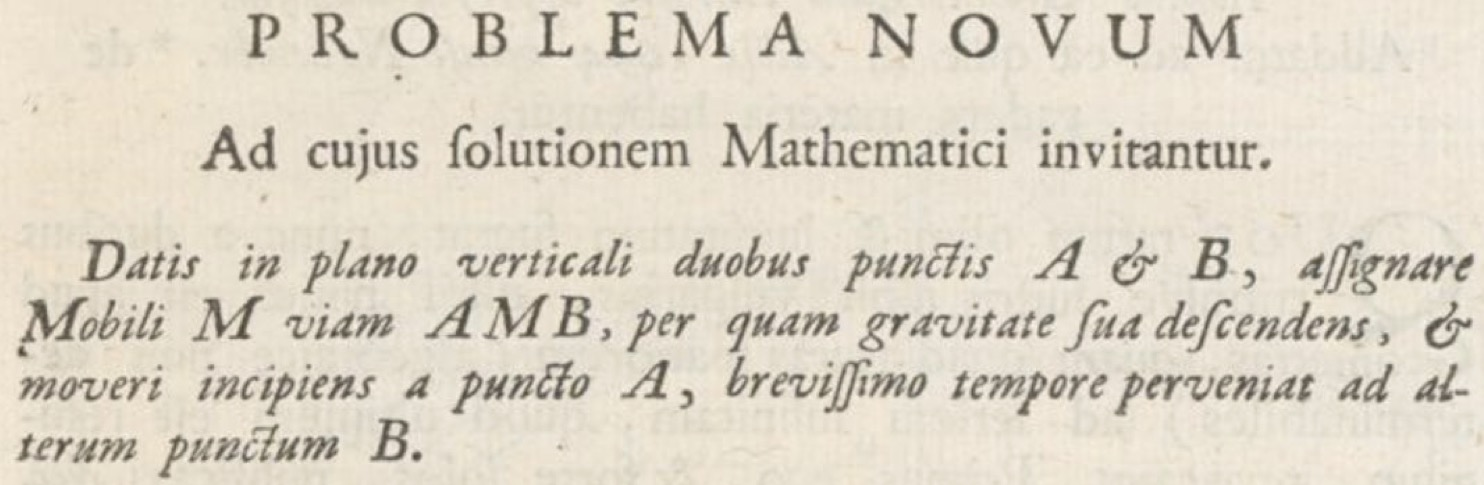
\includegraphics[width=0.8\textwidth]{chapters/020-variation/images/latein.jpg}
\end{center}
Zu deutsch:
\begin{quote}
Neue Aufgabe, zu deren Lösung die Mathematiker eingeladen werden.
Gegeben zwei Punkte $A$ und $B$ in einer vertikalen Ebene, finde
die Bahn $AMB$ eines Punktes $M$, der unter der Wirkung seines
Gewichtes in kürzester Zeit vom Punkt $A$ zum anderen Punkt $B$ absteigt.
\end{quote}
Die Situation der Aufgabenstellung ist in
Abbildung~\ref{buch:variation:fig:brachistochronenproblem}
dargestellt.
Bernoulli hat als Lösung gefunden, dass die Kurve eine Ausschnitt
aus einer Zykloide (in der Abbildung grau) sein muss.
Seine Lösung beruhte auf der Beobachtung, dass sich das Problem analog
zu einem Lichtausbreitungsproblem ist, für welches Fermat bereits
eine Lösung gefunden hat.

Da die Reibung vernachlässigt wird, ist die Energie des Massepunktes
erhalten.
Sie setzt sich aus der potenziellen und der kinetischen Energie
zusammen.
Die potenzielle Energie ist $-mgy$, die kinetische Energie ist
$\frac12mv^2$.
Die Energieerhaltung wird daher zu
\[
E=\frac12mv^2-mgy
\qquad\Rightarrow\qquad
v
=
\sqrt{2g}\!\sqrt{\frac{E}{gm}+y}
=
\!\sqrt{2(C+y)}.
\]
Durch Wahl einer anderen Zeiteinheit kann die Gleichung noch weiter
vereinfacht zu
\(
v = \sqrt{C+y}
\)
vereinfacht werden.
Gesucht ist also die zeitlich kürzeste Bahn eines Teilchens, 
dessen Geschwindigkeit auf bekannte Art $v(y)$ von der vertikalen
Koordinate abhängt.

%
% Das Fermat-Problem
%
\subsection{Das Fermat-Prinzip}
Bereits Fermat hat erkannt, dass das Brechnungsgesetz von Snellius
als Lösung eines Extremalproblems verstanden werden kann.

\begin{satz}[Fermat]
Sie $c/n_i$ die Geschwindigkeit, mit der sich Licht im Medium $M_i$
ausbreitet.
Ein Lichtstrahl von $A_1$ nach $A_2$ geht durch denjenigen Punkt $B$ 
auf der Grenzfläche zwischen den Medien, für den sich die Sinus der
Winkel $\alpha_i$ zwischen den Strahlen und der Normalen zur Grenzfläche
umgekehrt wie die $n_i$ verhalten, wenn also das Brechungsgesetz
\[
\frac{\sin\alpha_1}{\sin\alpha_2}
=
\frac{n_2}{n_1}
\]
gilt.
\end{satz}

\begin{proof}
Ohne der Beschränkung der Allgmeinheit können wir auf die Betrachtung
einer Ebene beschränken, die die beiden Punkte $A_i$ enthält und senkrecht
auf der Grenzfläche steht.
Wir dürfen weiter annehmen, dass die $x$-Achse in der Grenzfläche liegt 
und die Punkte $A_i$ die Koordinaten $(x_i,y_i)$ und der Punkt $B$ die
Koordinaten $(x,0)$ hat.
Es ist derjenige Punkt $x$ zu bestimmen, für den die Lichtzeit entlang 
des Pfades $A_1BA_2$ minimal wird.
Diese Zeit ist
\begin{align*}
t
&=
\frac{\overline{A_1B}}{c/n_1}
+
\frac{\overline{BA_2}}{c/n_2}
\\
ct
&=
n_1\overline{A_1B}
+
n_2\overline{A_2B}
\\
&=
n_1\!\sqrt{(x-x_1)^2 + y_1^2}
+
n_2\!\sqrt{(x_2-x)^2 + y_2^2}
\end{align*}
Das Minimum wird bei einer Nullstelle der Ableitung nach $x$ gefunden,
also bei einer Lösung der Gleichung
\begin{align*}
0
&=
n_1\frac{2(x_1-x)x}{\sqrt{(x_1-x)^2+y_1^2}}
+
n_2\frac{-2(x-x_2)x}{\sqrt{(x_2-x)^2+y_2^2}}.
\intertext{Indem man den zweiten Term auf der rechten Seite auf die linke
Seite bringt und durch $x$ dividiert, erhält man}
n_1
\frac{x_1-x}{\sqrt{(x_1-x)^2+y_1^2}}
&=
n_2
\frac{x-x_2}{\sqrt{(x_2-x)^2+y_2^2}}.
\end{align*}
Der Nenner ist auf beiden Seiten die Hypothenuse eines rechtwinkligen
Dreiecks, welches als Ankathete die Normale zur Grenzfläche hat.
Der Zähler ist die Gegenkathete des Winkels $\alpha_i$ zwischen der
Hypothenuse und der Normalen.
Daher ist der Quotient der Sinus des Winkels oder
\begin{equation}
n_1 \sin\alpha_1 = n_2 \sin\alpha_2.
\label{buch:variation:problem:eqn:snelliusinvariante}
\end{equation}
Die Gleichung~\eqref{buch:variation:problem:eqn:snelliusinvariante}
ist gleichbedeutend mit dem Brechungsgesetz
\[
\frac{\sin\alpha_1}{\sin\alpha_2}
=
\frac{n_2}{n_1}
\]
von Snellius.
\end{proof}

Der Satz von Fermat etabliert das Brechungsgsetz also Lösung eines
Extremalproblems.
Die Natur wählt für einen Lichtstrahl den zeitlich kürzesten Weg.
Der Beweis des Satzes von Fermat zeigt, dass entlang des Lichtstrahls
an jeder Grenzfläche zwischen Medien die Bedingung
\eqref{buch:variation:problem:eqn:snelliusinvariante}
erfüllt.
Wenn die optische Dichte $n$ eine Funktion von $n(y)$ ist, dann
wird der Lichtstrahl nicht nur in diskreten Punkten geknickt, sondern
entlang des ganzen Strahles gekrümmt.
Folgt der Strahl der Kurve $x(y)$, die mit der vertikalen den Winkel
$x'(y) = \tan\alpha(y)$ einschliesst.
Damit lässt sich auch die Sinus-Funktion ausdrücken, es gilt
\[
\sin\alpha(y)
=
\frac{x'(y)}{\pm\!\sqrt{x'(y)^2+1}}.
\]
Aus der Form~\eqref{buch:variation:problem:eqn:snelliusinvariante}
des Brechungsgesetztes wird dann die Gleichung
\begin{equation}
n_1\sin\alpha(y)
=
\frac{n_1(y)x'(y)}{\pm\!\sqrt{x'(y)^2+1}}
=
\operatorname{const}
\qquad\Rightarrow\qquad
\frac{n_1(y)^2x'(y)^2}{x'(y)^2+1}=C.
\label{buch:variation:eqn:fermatdgl}
\end{equation}
Dies ist eine Differentialgleichung für die Funktion $x(y)$.
Sie kann auch in die Form
\[
x'(y)^2
=
\frac{C}{(n_1(y)^2-C)}
\]
gebracht werden.

%
% Das Brachistochronenproblem als Lichtausbreitungsproblem
%
\subsubsection{Das Brachistochronenproblem als Lichtausbreitungsproblem}
Das Fermat-Prinzip besagt, dass ein Lichtstrahl, der sich in einem Medium
mit der Geschwindigkeit $c/n(y)$ ausbreitet, die Gleichung 
\eqref{buch:variation:eqn:fermatdgl} erfüllt.
Beim Brachistochronenproblem ist die Geschwindigkeit $v(y)=\!\sqrt{C-y}$ und 
damit $n(y) = c/\!\sqrt{C-y}$.
Eine Brachistochrone ist also eine Kurve, die die aus
\eqref{buch:variation:eqn:fermatdgl} folgende Gleichung
\begin{equation}
\frac{x'(y)^2}{(1+x'(y)^2)(C-y)} = K
\label{buch:variation:problem:eqn:bernoullidgl}
\end{equation}
erfüllen.

%
% Die Bernoullische Lösung
%
\subsubsection{Die Bernoullische Lösung}
Bernoulli hat gefunden, dass die Brachistochrone ein Zykloidenbogen ist.
Dies lässt sich dadurch verifizieren, dass man die Parametrisierung
einer Zykloide in die
Gleichung~\eqref{buch:variation:problem:eqn:bernoullidgl}
einsetzt.
Die Zykloide hat die Parametrisierung
\[
\left.
\begin{aligned}
x &= r(\varphi - \sin\varphi) 
\\
y &= r(1-\cos\varphi)
\end{aligned}
\right\}
\quad
\text{mit der Ableitung}
\quad
\left\{
\begin{aligned}
\dot{x}(\varphi) &= r(1-\cos\varphi)\\
\dot{y}(\varphi) &= r\sin\varphi
\end{aligned}
\right.
\]
für $\varphi\in\mathbb{R}$.
Die Ableitung ist
\[
x'(y)
=
\frac{\dot{x}(\varphi)}{\dot{y}(\varphi)}
=
\frac{1-\cos\varphi}{\sin\varphi}.
\]
Eingesetzt in \eqref{buch:variation:problem:eqn:bernoullidgl}
wird daraus
\[
\frac{\dot{x}(\varphi)^2}{
(\dot{y}(\varphi)^2 +\dot{x}(\varphi)^2)
(C-r(1-\cos\varphi))
}
=
\frac{(1-\cos\varphi)^2}{
((1-\cos\varphi)^2+\sin^2\varphi)
(C-r+r\cos\varphi)
}
=
K.
\]
Ausmultiplizieren im Nenner ergibt
\[
\frac{(1-\cos\varphi)^2}{
(1-2\cos\varphi+\cos^2\varphi+\sin^2\varphi)
(C-r+r\cos\varphi)
}
=
\frac{1-\cos\varphi}{
2(C-r+r\cos\varphi)
}
\]

%
% Das Brachistochronenproblem als Variationsproblem
%
\subsection{Das Brachistochronenproblem als Variationsproblem
\label{buch:variation:problem:subsection:variationsproblem}}
Die Bernoullische Lösung des Brachistochronenproblems verwendet die
Analogie zum Fermat-Prinzip.
Eine solche Analogie ist nur selten möglich, daher soll das Problem
jetzt in eine Form gebracht werden, in die auch viele ähnliche
Optimierungsproblem gebracht werden können.

Wir erinnern daran, dass die Geschwindigkeit des Massepunktes durch
$v(y)=\sqrt{C-y}$ gegeben ist.
Damit lässt sich die Zeit berechnen, die der Massepunkt entlang der
Lösungskurve braucht, wenn man diese als Funktion $y(x)$ mit beschreibt.
Die Punkte $A$ und $B$ sollen die $x$-Koordinaten $a$ bzw.~$b$ haben.
Für das Kurvenstück zwischen den $x$-Koordinaten $x$ und $x+\Delta x$
braucht der Massepunkt die Zeit
\[
\frac{ \sqrt{\Delta x^2 + \Delta y^2} }{v(y)}
=
\frac{ \sqrt{1 + y'(x)^2} }{ v(y) } \Delta x.
\]
Die Zeit ist das Integral
\begin{equation}
t
=
\int_a^b \frac{\sqrt{1+y'(x)^2}}{v(y(x))}\,dx
=
\int_a^b \sqrt{\frac{1+y'(x)^2}{C-y(x)}}\,dx.
\label{buch:variation:problem:eqn:brachint}
\end{equation}
Der Integrand auf der rechten Seite hängt nur von den Funktion $y(x)$
und $y'(x)$ ab.
Dies kommt vor allem daher, dass die Geschwindigkeit nur von $y$ abhängt,
nicht auch noch von $x$.
Im Allgemeinen wird man also davon ausgehen müssen, dass der Integrand
auch noch von $x$ abhängt.
Die Variationsrechnung befasst sich mit Problemen, in denen Funktionen
gefunden werden müssen, die ein Integral wie das in
\eqref{buch:variation:problem:eqn:brachint}
minimiert oder maximiert werden müssen.

\begin{definition}[Lagrange-Funktion des Brachistochronenproblems]
Die Lagrange-Funk\-tion des Brachistochronenproblems ist der
Integrand des Integrals
\eqref{buch:variation:problem:eqn:brachint},
\index{Lagrange-Funktion}%
also die Funktion
\[
L(x,y,y')
=
\sqrt{\frac{1+y^{\prime 2}}{C-y}}.
\]
\end{definition}

%
% Funktionale
%
\subsection{Funktionale
\label{buch:variation:problem:subsection:funktionale}}
Die Variationsrechnung löst Optimierungsproblem, die von einer
Funktion abhängen.
Um dies mathematisch präzis zu fassen, ist zunächst nötig, die Menge
der in Frage kommenden Funktionen so einzuschränken, dass die interessierende
Grösse überhaupt wohldefiniert ist.

%
% Vektorräume
%
\subsubsection{Vektorräume}
Zunächst sind die gemeinsamen algebraischen Eigenschaften zu charakterisieren,
die wir von den für unsere Untersuchungen zweckmässigen Funktionenmengen
erwarten.

\begin{definition}[Vektorraum]
Ein Vektorraum über den reellen Zahlen $\mathbb{R}$ ist einem Menge $V$ mit
zwei Operationen, der Addition und der Multiplikation mit Skalaren
\begin{align*}
    +\colon V\times V         &\to V : (u,v)\mapsto u+v
&
\cdot\colon \mathbb{R}\times V&\to V : (\lambda,v) \mapsto\lambda v
\end{align*}
mit den folgenden Eigenschaften.
\begin{enumerate}
\item
Es gelten die Assoziativgesetze
\begin{align*}
(u+v)+w&=u+(v+w)&&\text{für alle $u,v,w\in V$}\\
(\lambda \mu)v&=\lambda(\mu v)&&\text{für alle $\lambda,\mu\in\mathbb{R},\;v\in V$.}
\end{align*}
\item
Es gibt einen Vektor $0\in V$ mit der Eigenschaft $0+v=v$ für alle
Vektoren $v\in V$.
\item
Zu jedem Vektor $v\in V$ gibt es den entgegengesetzten Vektor $-v\in V$
mit der Eigenschaft, dass $-v+v=0$ ist.
\item
Die Addition von Vektoren ist kommutativ: $u+v=v+u$ für alle $u,v\in V$.
\item
Es gelten die Distributivgesetze 
\begin{align*}
(\lambda + \mu) v &= \lambda v + \mu v
	&\quad\text{für alle $\lambda,\mu\in\mathbb{R},\;v\in V$}\\
\lambda(u+v)      &= \lambda u + \lambda v
	&\quad\text{für alle $\lambda\in\mathbb{R},\;u,v\in V$}
\end{align*}
\end{enumerate}
\end{definition}

Die Mengen $\mathbb{R}^n$ erfüllen die genannten Eigenschaften, sind
also Vektorräume.
Die Definition eines Vektorraums ist aber viel allgemeiner, insbesondere
gehören dazu auch Mengen von Funktionen.
Damit wird es möglich, die Berechnungen in $\mathbb{R}^n$ auf Funktionen
auszudehnen.
Zum Beispiel bilden die stetigen Funktionen auf einem Intervall einen
Vektorraum, wie das folgende Beispiel zeigt.

\begin{beispiel}
Die Menge
\[
C([a,b])
=
\{f\colon[a,b]\to\mathbb{R}\mid \text{$f$ ist stetig}\}
\]
der stetigen Funktionen bildet einen Vektorraum.
Die Operationen sind die punktweise Addition von Funktionen und die
Multiplikation der Werte mit Skalaren, für $f,g\in C([a,b])$ und
$\lambda\in \mathbb{R}$ ist
\begin{align*}
(f+g)(x) &= f(x)+g(x)
&&\text{und}&
(\lambda f)(x) &= \lambda f(x).
\end{align*}
Entscheidend ist, dass die Addition von Funktionen und die Multiplikation
mit Skalaren nicht aus der Menge herausführt.
Tatsächlich wird in der Analysis gezeigt, dass die Summe stetiger Funktionen
wieder stetig ist und dass die Funktion $x\mapsto \lambda f(x)$ stetig,
wenn $f$ stetig ist.
Die übrigen Eigenschaften sind ebenfalls erfüllt, da sie bereits für die
Funktionswerte erfüllt sind.
\end{beispiel}

%
% Norm und Grenzwerte
%
\subsubsection{Norm und Grenzwerte}
Um Analysis zu betreiben, muss man ausdrücken können, dass eine Folge
von Funktionen konvergiert.
Dazu ist ein Abstandsbegriff zwischen Funktionen nötig.

\begin{definition}[Norm, normierter Raum]
Eine {\em Norm} auf einem Vektorraum $V$ ist eine Abbildung
\index{Norm}%
$\|\cdot\|\colon V\to\mathbb{R}^+_0$ mit nichtnegativen reellen Werten
und den folgenden Eigenschaften
\begin{itemize}
\item Definitheit: $\|v\|\ge 0$ für $v\in V$ mit Gleichheit 
genau dann, wenn $v=0$.
\index{Definitheit}%
\item Absolute Homogenität: Für alle Vektoren $v\in V$ und
\index{Homogenität}%
$\lambda\in\mathbb{R}$ gilt $\|\lambda v\| = |\lambda|\, \|v\|$.
\item Dreiecksungleichung: für alle Vektoren $u,v\in V$ gilt
\index{Dreiecksungleichung}%
$\|u+v\|\le \|u\|+\|v\|$.
\end{itemize}
Ein {\em normierter Raum} ist ein Vektorraum mit einer Norm.
\index{normierter Raum}%
\end{definition}

\begin{beispiel}
Der Vektorraum der stetigen Funktionen kann mit der Supremum-Norm
\[
\|f\| = \sup_{x\in[a,b]} |f(x)|
\]
zu einem normierten Raum gemacht werden.
Die Definitheit ist durch die Definition offensichtlich sichersgtellt.
Für $\|\lambda f\|$ finden wir
\[
\|\lambda f\|
=
\sup_{x\in[a,b]} |\lambda f(x)|
=
|\lambda|\,
\sup_{x\in[a,b]} |f(x)|
=
|\lambda|\, \|f\|,
\]
was die Homogenität zeigt.
Die Dreiecksungleichung folgt aus
\begin{align*}
\|f+g\|
&=
\sup_{x\in[a,b]} |f(x)+g(x)|
\\
&\le
\sup_{x\in[a,b]} (|f(x)|+|g(x)|)
\\
&\le
\sup_{x\in[a,b], y\in[a,b]} (|f(x)|+|g(y)|)
\\
&=
\sup_{x\in[a,b]} |f(x)|
+
\sup_{y\in[a,b]} |g(y)|
=
\|f\| + \|g\|.
\qedhere
\end{align*}
\end{beispiel}

Mit einer Norm ist es jetzt möglich, die Konvergenz von Folgen und den
Begriff des Grenzwertes zu definieren.

\begin{definition}[Cauchy-Folge, Grenzwert]
Eine Folge $(x_n)_{n\in\mathbb{N}}$ in $V$ in einem normierten Raum $V$
mit der Norm $\|\cdot\|$
heisst eine Cauchy-Folge, wenn es für jedes $\varepsilon>0$ eine
\index{Cauchy-Folge}%
$N\in \mathbb{N}$ gibt derart, dass
\[
\| x_n - x_m \| < \varepsilon
\quad\forall n,m\ge N.
\]
Der Vektor $x\in V$ heisst {\em Grenzwert} der Folge $(x_n)_{n\in\mathbb{N}}$,
\index{Grenzwert}%
wenn es zu jedem $\varepsilon > 0$ ein $N\mathbb{N}$ gibt derart, dass
\[
\|x_n-x\| < \varepsilon 
\quad\forall n\ge N.
\]
Die Folge $(x_n)_{n\in\mathbb{N}}$  in $V$ heisst {\em konvergent}, wenn
\index{konvergent}%
$x$ der Grenzwert von $(x_n)_{n\in\mathbb{N}}$ ist.
\end{definition}

Der durch die Supremum-Norm definierte Konvergenzbegriff ist die gleichmässige
Konvergenz.
Zur Erinnerung:
Eine Folge $f_n$ von Funktionen heisst gleichmässig konvergent gegen die
Funktion $f$, wenn es zu jedem
$\varepsilon >0$ ein $N\in\mathbb{N}$ gibt derart, dass
\[
|f_n(x) - f(x)|<\varepsilon\quad\forall n>N\text{ und }x\in [a,b].
\]
Die Supremum-Norm ist
\[
\|f_n(x) - f(x)\|
=
\sup_{x\in[a,b]} |f_n(x)-f(x)| < \varepsilon
\]
für alle $n>N$.
Dies ist genau die Konvergenz in der Norm $\|\cdot\|$.
Aus der Analysis ist bekannt, dass eine gleichmässig konvergente 
Funktionenfolge gegen eine stetige Funktion konvergiert.

\begin{definition}[Banach-Raum]
Ein normierter Raum $V$ heisst ein {\em Banach-Raum},
\index{Banach-Raum}%
wenn jede Cauchy-Folge in $V$ einen Grenzwert hat.
\end{definition}

\begin{beispiel}
Die Menge $C^1([0,2])$
der stetigen Funktionen auf dem Intervall $[0,2]$ ist ein normierter
Raum mit der Norm
\[
\|f\|_1
=
\int_0^2 |f(x)|\,dx,
\]
die auch die $L^1$-Norm heisst.
\index{L1-Norm@$L^1$-Norm}%
Zunächst ist nachzuprüfen, dass dies tatsächlich eine Norm ist.
Die Definitheit und die Homogenität von $\|\cdot\|_1$ ist klar, nur
die Dreiecksungleichung erfordert etwas Arbeit.
Für Funktionen $f,g\in L^1([0,2])$ gilt
\begin{align*}
\|f+g\|_1
&=
\int_0^2 |f(x)+g(x)|\,dx
\\
&\le 
\int_0^2 |f(x)|+|g(x)|\,dx
=
\int_0^2 |f(x)|\,dx
+
\int_0^2 |g(x)|\,dx
=
\|f\|_1+\|g\|_1,
\end{align*}
was die Dreeicksungleichung beweist.

Eine Cauchy-Folge in der $L^1$-Norm muss aber nicht unbedingt einen
stetigen Grenzwert haben.
Die Funktionen
\(
f_n(x) =
\begin{cases}
x^n&\quad x< 1\\
1&\quad x\ge 1
\end{cases}
\)
haben die $L^1$-Norm
\begin{align*}
\|f_n-f_m\|_1
=
\int_0^2 |f_n(x)-f_m|\,dx
\\
&=
\biggl|\int_0^1 x^n-x^m\,dx\biggr|
=
\biggl[
\biggl|
\frac{1}{n+1}x^{n+1}
-
\frac{1}{m+1}x^{m+1}
\biggr|
\biggr]_0^1
\\
&=
\biggl|
\frac{1}{n+1}
-
\frac{1}{m+1}\biggr|.
\end{align*}
Wegen
\[
\|f_n-f_m\|_1
<\varepsilon
\]
für $n,m>2/\varepsilon$ ist $f_n$ eine Cauchy-Folge in $L^1$.
In $L^1$ konvergiert die Folge $f_n$ gegen die Funktion
\[
f(x)
=
\begin{cases}
0&\quad x< 1\\
1&\quad x\ge 1.
\end{cases}
\]
Diese Funktion ist aber nicht stetig, da sie bei $x=1$ einen
Sprung hat.
Bezüglich der $L^1$-Norm ist $C^1([a,b])$ als im Allgemeinen
kein Banach-Raum.
\end{beispiel}

%
% Stetige und differenzierbare Funktionen
%
\subsubsection{Stetige und differenzierbare Funktionen}
Mit der Norm lässt sich auch die Stetigkeit von Abbildungen zwischen
normierten Räumen definieren.

\begin{definition}[Stetigkeit]
Eine Funktion $f\colon U\to V$ zwischen normierten Räumen heisst
{\em stetig im Punkt} $x\in U$, wenn es zu jedem $\varepsilon > 0$
\index{stetig in einem Punkt}%
ein $\delta > 0$
gibt derart, dass
\(
\|f(x)-f(y)\| < \delta
\)
wenn
\(
\|x-y\|<\varepsilon
\).
Eine Funktion $f\colon U\to V$ heisst {\em stetig}, wenn sie in
jedem Punkt von $U$ stetig ist.
\end{definition}

Das Bild einer Folge $x_n\in U$, die gegen $x_0\in U$ konvergiert,
ist eine Folge $f(x_n)$ in $V$.
Man sagt, $y\in V$ sei der Grenzwert von $f(x)$ für $x\to x_0$,
wenn $f(x_n)$ für jede solche Folge $x_n$ gegen $y$ konvergiert.
Der Grenzwert wird auch
\[
\lim_{x\to x_0} f(x)
=
y
\]
geschrieben.
Stetige Funktionen zeichnen sich wie in der Analysis der Funktionen
einer Variablen dadurch aus, dass der Grenzwert der Werte der Funktion
auf einer konvergenten Folge mit dem Funktionswert des Grenzwertes
übereinstimmt.

\begin{satz}
Eine Funktion $f\colon U\to V$ ist genau dann stetig im Punkt $x\in U$,
wenn für jede Folge $x_n$ in $U$ mit Grenzwert $x$ die Folge $f(x_n)$
konvergent ist und
\[
\lim_{n\to\infty} f(x_n) = f(x).
\]
Eine lineare Funktion $f\colon U\to V$ ist genau dann stetig,
wenn für jede Nullfolge $x_n$ in $U$ 
\[
\lim_{n\to \infty} f(x_n) = 0
\]
gilt.
\end{satz}

\begin{definition}
Eine Funktion $f\colon U\to V$ zwischen normierten Räumen heisst
differenzierbar im Punkt $x\in U$ wenn es eine lineare Funktion
$Df(x_0)\colon U\to V$ gibt derart, dass
\[
f(x+v) =f(x) + Df(x_0)\cdot v + o(v),
\]
wobei $o(v)$ bedeutet, dass für diese Funktion
\[
\frac{o(v)}{|v|}\to 0
\quad\text{für $v\to 0$}
\]
gilt.
\end{definition}

Funktionen auf einem Vektorraum mit reellen Werten weren auch
{\em Funktionale} genannt.
\index{Funktional}
Vor dem 20.~Jahrhundert wurde häufig ein Untersschied zwischen
Funktionen von endlich vielen reellen Variablen und Funktionen
von einem unendlichdimensionalen Vektorraum gemacht.
Die Entwicklungen dieses  Abschnittes haben gezeigt, dass eine
solche Unterscheidung nicht gerechtfertigt ist.
Es ist lediglich notwendig, die Definitionen allgemein genug zu
fassen und sich jederzeit über die Funktionenmenge und die zu
verwendende Norm Rechenschaft abzulegen.


%
% 2-fundamtenallemma.tex
%
% (c) 2023 Prof Dr Andreas Müller
%
\section{Das Fundamentallemma
\label{buch:variation:section:fundamentallemma}}
\kopfrechts{Das Fundamentallemma}
Im Fall des endlichdimensionalen Extremalproblems ist aus der
Forderung, dass alle Richtungsableitung verschwinden müssen, 
die Bedingung geworden, dass
\[
v\cdot\grad f = 0
\]
sein muss für alle Vektoren $v\in\mathbb{R}^n$.
Wir haben daraus geschlossen, dass der Gradient $\grad f=0$
sein muss.
Wir hatten dies das endlichdimensionale Fundamentallemma genannt,
wegen $e_k\cdot \grad f = D_kf$ war es eine ziemliche Selbstverständlichkeit.
Bei der Lösung von Variationsproblemen, wo es nicht um endlichdimensionale
Vektoren und das Skalarprodukt, sondern um Funktionen und Integrale
geht, brauchen wir eine ähnliche Aussage für Funktionen.

%
% Positive glatte Funktionen mit kompaktem Träger
%
\subsection{Positive glatte Funktionen mit kompaktem Träger}
Die Aussage des Fundamentallemmas für endlichdimensionale Vektoren 
folgte sofort aus der Tatsache, dass es für jedes $k$ einen Vektor
$e_k$ gibt, der nur in der Koordinaten $k$ von $0$ verschieden ist.
Natürlich gibt es auch Funktionen, die nur in genau einem Punkt
von $0$ verschieden sind.
Eine solche Funktion ist aber im allgemeinen nicht differenzier-
oder integrierbar.
In diesem Abschnitt soll daher gezeigt werden, dass es unendlich
oft stetig differnzierbare Funktionen gibt, die nur in einem beliebig
kleinen vorgegebenen Intervall $\ge 0$ sind.

\begin{definition}[Träger]
Der {\em Träger} einer Funktion $f\colon X\to\mathbb{R}$ ist die Menge
\index{Träger}%
\[
\supp f = \{ x\in X\mid f(x)\ne \}.
\]
\end{definition}

Gesucht ist also eine beliebig oft stetig differenzierbare Funktion,
deren Träger in einem vorgegebenen Intervall $[a,b]$ enthalten ist.
Wir konstruieren so eine Funktion in zwei Schritten.

\input{chapters/020-variation/fig/f.tex}

\begin{satz}
\label{buch:variation:fundamentallemma:satz:glatt}
Die Funktion
\[
f(x)
=
\begin{cases}
e^{-1/x}&\qquad x>0\\
0&\qquad x\le 0
\end{cases}
\]
(siehe auch Abbildung~\ref{buch:variation:fundamentallemma:fig:glatt})
ist beliebig oft stetig differenzierbar.
\end{satz}

\begin{proof}
Es ist klar, dass die Funktion $f$ beliebig oft stetig differenzierbar
ist in jedem Punkt $x\ne 0$.
Es ist also nur nachzuweisen, dass $f(x)$ im Punkt $0$ beliebig
oft stetig differenzierbar ist.

Die ersten drei Ableitungen von $f(x)$ sind
\begin{align}
f'(x) &= \frac{1}{x^2} f(x)
\label{buch:variation:fundamentallemma:eqn:f1}
\\
f''(x) &= \frac{1-2x}{x^4}f(x)
\notag
\\
f'''(x) &= \frac{6x^2-6x+1}{x^6}f(x).
\notag
\end{align}
Daraus lässt sich die Vermutung ableiten, dass
\begin{equation}
f^{(n)}(x)
=
\frac{p_{n-1}(x)}{x^{2n}} f(x)
\label{buch:variation:fundamentallemma:eqn:fabl}
\end{equation}
ist, wobei $p_k(x)$ ein Polynom vom Grad $k$ ist.
Wir beweisen diese Vermutung mit Hilfe von vollständiger Induktion.
Die Induktionsverankerung für die $0$-te Ableitung ist trivial.

Wir nehmen jetzt im Sinne der Induktionsannahme an, dass die $n$-te
Ableitung die Form \eqref{buch:variation:fundamentallemma:eqn:fabl}
hat.
Wir müssen zeigen, dass dann auch $f^{(n+1)}(x)$ diese Form hat.
Dazu berechnen wir
\begin{align}
f^{(n+1)}(x)
&=
\frac{d}{dx}
\frac{p_n(x)}{x^{2n}} f(x)
\notag
\\
&=
\frac{p_n'(x)}{x^{2n}} f(x)
-2n
\frac{p_n(x)}{x^{2n+1}} f(x)
+
\frac{p_n(x)}{x^{2n}} f'(x).
\notag
\intertext{Mit der ersten Ableitung
\eqref{buch:variation:fundamentallemma:eqn:f1} wird dies zu}
&=
\frac{p_n'(x)}{x^{2n}} f(x)
-2n
\frac{p_n(x)}{x^{2n+1}} f(x)
+
\frac{p_n(x)}{x^{2n}} \frac{1}{x^2}f(x)
\notag
\\
&=
\frac{x^2p_n'(x) -2nxp_n(x)+p_n(x)}{x^{2n+2}} f(x).
\label{buch:variation:fundamentallemma:eqn:induktionsschritt}
\end{align}
Die Ableitung $p_n'(x)$ ist ein Polynom vom Grad $n-1$ und damit
ist $x^2p_n'(x)$ ein Polynom vom Grad $n+1$.
Ebenso ist $xp_n(x)$ ein Polynom vom Grad $n+1$ während
$p_n(x)$ ein Polynom vom Grad $n$ ist.
Der Zähler von
\eqref{buch:variation:fundamentallemma:eqn:induktionsschritt}
ist
\[
p_{n+1}(x)
=
x^2p_n'(x)+(1 -2nx)p_n(x),
\]
ein Polynom vom Grad $n+1$.
Damit ist der Induktionsschritt erfolgreich und die Behauptung betreffend
die Form von $f^{(n)}(x)$ ist bewiesen.

Es ist jetzt nur noch zu zeigen, dass der Grenzwert von $f^{(n)}(x)$
für $x\to 0+$ verschwindet.
Da das Polynom $p_n(x)$ stetig ist, folgt
\[
\lim_{x\to 0}
f^{(n)}(x)
=
\lim_{x\to 0}\frac{p_n(x)}{x^{2n}}f(x)
=
p_n(0) \lim_{t\to\infty} t^{2n} e^{-t}
=
0.
\]
Damit ist die beliebige stetige Differenzierbarkeit an der Stelle
$x=0$ gezeigt.
\end{proof}

Die Funktion $f(x)$ von 
Satz~\ref{buch:variation:fundamentallemma:satz:glatt} 
erfüllt noch nicht die Forderung, dass sie nur in einem vorgegebenen
Intervall von $0$ verschieden ist.

\input{chapters/020-variation/fig/g.tex}

\begin{satz}
\label{buch:variation:fundamentallemma:satz:gab}
Sei $f(x)$ die Funktion von
Satz~\ref{buch:variation:fundamentallemma:satz:glatt}.
Dann ist
\[
g_{a,b}(x)
=
f(x-a) f(b-x)
\]
eine unendlich oft stetig differenzierbare, nichtnegative Funktion mit Träger
$\supp g_{a,b}=(a,b)$.
\end{satz}

Die Funktionen $g_{a,b}(x)$ sind beliebig oft differenzierbar und nur im
Intervall $[a,b]$ von $0$ verschieden und sogar positiv.
Weil sie stetig sind, sind sie auch integrierbar, man kann also das
Integral über $\mathbb{R}$ berechnen und die Funktion damit normieren.
Die neue Funktion
\[
\frac{1}{N}
\tilde{g}_{a,b}(x)
\qquad\text{mit}\;
N
=
\int_{-\infty}^{\infty}g_{a,b}(x)\,dx
=
\int_a^b g_{a,b}(x)\,dx
\]
ist immer noch beliebig oft stetig differenzierbar und hat zusätzlich die
Eigenschaft
\[
\int_{-\infty}^{\infty}
\tilde{g}_{a,b}(x)\,dx
=
\int_a^b
\tilde{g}_{a,b}(x)\,dx
=
1.
\]
Wir formulieren dieses Resultat als Satz.

\begin{satz}
\label{buch:variation:satz:gabeins}
Zu jedem Intervall $[a,b]$ gibt es eine beliebig oft stetig
differenzierbare Funktion $g(x)$, genau das Intervall $[a,b]$
als Träger hat und deren Integral über $[a,b]$ den Wert $1$ hat.
\end{satz}

%
% Das Fundamentallemma
%
\subsection{Das Fundamentallemma}
Mit der Funktion $g_{a,b}(x)$ von
Satz~\ref{buch:variation:fundamentallemma:satz:gab}
lässt sich jetzt das Fundamentallemma in der folgenden Form
leicht beweisen.

\begin{satz}[Fundamentallemma]
\label{buch:variation:fundamentallemma:satz:fundamentallemma}
Wenn für die stetige Funktion $f\colon[a,b]\to\mathbb{R}$ 
\begin{equation}
\int_a^b f(x)\varphi(x)\,dx = 0
\label{buch:variation:fundamentallemma:eqn:fundamentalbed}
\end{equation}
gilt für jede beliebig oft stetig differenzierbare Funktion $\varphi(x)$ 
dann ist $f(x)=0$.
Das Resultat gilt selbst dann, wenn
\eqref{buch:variation:fundamentallemma:eqn:fundamentalbed}
nur für beliebig oft stetig differenzierbare Funktionen $\varphi(x)$ 
gilt, die ausserdem an den Intervallenden verschwinden:
$\varphi(a)=\varphi(b)=0$.
\end{satz}

\begin{proof}
Wir zeigen mit Hilfe eines Widerspruchs, dass es keinen Punkt $x_0\in[a,b]$
geben kann, für den $f(x_0)\ne 0$ ist.
Dazu nehmen wir also an, dass $f(x_0)\ne 0$ ist.
Falls $f(x_0)<0$ ist, ersetzen wir $f$ durch $-f$, 
die Bedingung
\eqref{buch:variation:fundamentallemma:eqn:fundamentalbed}
ändert sich dadurch nicht.
\input{chapters/020-variation/fig/fundamentallemma.tex}
Wir dürfen daher annehmen, dass $f(x_0)>0$ ist
(Abbildung~\ref{buch:variation:fundamentallemma:fig:beweis}).
Da $f$ stetig ist, gibt es ein Intervall $[x_0-\varepsilon,x_0+\varepsilon]$
derart, dass $f(x)> \frac12 f(x_0)$ für
$x\in[x_0-\varepsilon,x_0+\varepsilon]$ gilt.
Dann gilt für das Integral
\[
\int_a^b
f(x)
g_{x_0-\varepsilon,x_0+\varepsilon} (x)
\,dx
>
\frac{f(x_0)}{2}
\int_a^b
g_{x_0-\varepsilon,x_0+\varepsilon} (x)
\,dx
>
0
\]
im Widerspruch zur Bedingung
\eqref{buch:variation:fundamentallemma:eqn:fundamentalbed}.
Der Widerspruch zeigt, dass $f(x)=0$ sein muss.
\end{proof}

%
% Skalarproduktformulierung des Fundamentallemmas
%
\subsection{Skalaproduktformulierung des Fundamentallemmas}
Die Richtungsableitung einer Funktion endlich vieler Variablen 
konnte als Skalarprodukt mit dem Gradienten geschrieben werden und
das Fundamentallemma hat besagt, dass der Gradient verschwindet,
wenn alle Richtungsableitungen verschwinden.
Diese Schlussweise ist auch für Funktionen möglich, wenn man Funktionen
ein Skalarprodukt definieren kann.

\begin{definition}[$L^2$-Skalarprodukt]
Das {\em Skalarprodukt} zweier quadratintegrierbarer Funktion $f$ und $g$
auf dem Intervall $[a,b]$ ist definiert durch
\[
\langle f,g\rangle
=
\int_a^b f(x)g(x)\,dx.
\]
\end{definition}

\begin{satz}[Fundamentallemma, Skalarproduktform]
Wenn für eine stetige Funktion $f\colon[a,b]\to\mathbb{R}$ das Skalarprodukt
\[
\langle f,\varphi\rangle = 0
\]
ist für jede unendlich oft differenzierbare Funktion $\varphi$ auf dem
Intervall $[a,b]$, dann ist $f=0$.
\end{satz}



%
% 3-eulerlagrange.tex
%
% (c) 2023 Prof Dr Andreas Müller
%
\section{Die Euler-Lagrange Differentialgleichung
\label{buch:variation:section:eulerlagrange}}
\kopfrechts{Die Euler-Lagrange Differentialgleichung}
Das Neuartige an der Aufgabenstellung des Brachistochronenproblems
war, dass eine Funktion gesucht war, so dass ein damit gebildetes
Integral eine Minimaleigenschaft erfüllt.
Für die damalige Mathematik war die Aufgabe, eine Funktion zu finden,
nicht neu.
Die Theorie der Differentialgleichungen war bereits entwickelt,
Newton hat die Infinitesimalrechnung ja erfunden, um damit die
Bewegungsgleichungen der Physik zu formulieren und zu lösen.
In einer Differentialgleichung werden Werte und Ableitungen einer
Funktion an einer einzigen Stelle miteinander verbunden.
Etwas salop formuliert sagt die Differentialgleichung in jedem
Punkt, in welche Richtung und mit welcher Krümmung die Funktionskurve
weiter zu zeichnen ist.

Im Brachistochronenproblem tragen aber alle Werte der gesuchten
Funktion zum Integral bei, es scheint daher auf den ersten Blick
nicht möglich, das Problem durch schrittweise Konstruktion
``von Punkt zu Punkt'' der Lösungskurve zu konstruieren.

Bernoullis Lösung des Brachistochrononproblems beruht auf der
Beobachtung, dass sich die Bedinung für die schnellste Bahn
durch eine Bedingung ersetzen lässt, die in jedem einzelnen
Punkt ausgewertet werden kann.
Das von ihm verwendete Fermat-Prinzip wurde ursprünglich ebenfalls
als eine globale Eigenschaft eines Lichtstrahls formuliert.
Aus dem Fermat-Prinzip folgt aber das Brechungsgesetz, welches
sagt, dass die Richtung eines Strahls in einem Punkt genau dann
ändert, wenn sich dort auch der Brechungsindex der beiden Medien
ändert.
Das Fermat-Prinzip ist also ein Beispiel dafür, wie eine globale
Bedingung erfüllt werden kann, indem einer lokalen Regel in jedem
Punkt gefolgt wird.

Es ist das Verdienst von Euler und Lagrange, zu erkennen, dass diese
Übersetzung eines globalen Variationsproblems in ein lokales 
Problem immer möglich ist.
Es entsteht dabei die Euler-Lagrange-Differentialgleichung, welche
die Problemstellung auf die Lösung einer Differentialgleichung
reduziert.
Damit ist ein allgemein anwendbares Lösungsverfahren gefunden.
Zu einem Variationsproblem lässt sich immer eine Differentialgleichung
finden, welche die gesuchte Funktion als Lösung hat.

In diesem Abschnitt soll dieser indirekte Weg der Lösung von
Variationsaufgaben dargestellt werden.
Wir werden später zeigen, dass diese Vorgehensweise nicht immer
erfolgreich sein kann.
Zum Beispiel werden wir in Kapitel~\ref{buch:chapter:nichtdiff}
Variationsprobleme kennenlernen, deren Lösungskurven nicht
differenzierbar sind und daher auch nicht von einer Differentialgleichung
gefunden werden können.
Im Kapitel~\ref{buch:chapter:direkt} werden daher die sogenannten
direkten Methodn vorgestellt, die den Umweg über eine
Differentialgleichung vermeiden.

%
% Die Lagrange-Funktion
%
\subsection{Die Lagrange-Funktion
\label{buch:variation:eulerlagrange:subsection:lagrange-funktion}}
Wir betrachten Variationsproblem der folgenden Art.
Gesucht ist eine auf dem Intervall $[x_0,x_1]$ definirte
Funktion $y(x)$, die das Integral
\begin{equation}
I(y)
=
\int_{x_0}^{x_1}
F(x, y(x), y'(x))
\,dx
\label{buch:variation:eulerlagrange:eqn:funktional}
\end{equation}
maximiert oder minimiert.
Der Ausdruck~\eqref{buch:variation:eulerlagrange:eqn:funktional}
wird ein Funktional genannt.
Die Funktion
\[
F
\colon
\mathbb{R}\times
\mathbb{R}\times
\mathbb{R}
\to
\mathbb{R}
\]
von drei Variablen heisst die {\em Lagrange-Funktion}
des Funktionals \eqref{buch:variation:eulerlagrange:eqn:funktional}.

\begin{beispiel}
Die Lagrange-Funktion des Brachistochronenproblems ist
\[
F(x,y,y')
=
\sqrt{ \frac{1+y^{\prime 2}}{y} }.
\]
Die Funktion hängt nicht von $x$ ab, was bedeutet, dass eine
Verschiebung in $x$-Richtung die Form der Lösungsfunktion des
Variationsproblems nicht ändert.
\end{beispiel}

\begin{beispiel}
\label{buch:variation:eulerlagrange:beispiel:gerade}
Wir formulieren die Aufgabe, die kürzeste Verbindung der Punkte
$(x_0,y_0)$ und $(x_1,y_1)$ in einer Ebene zu finden, als Variationsproblem.
Die Länge einer Kurve $y(x)$ ist das Integral
\[
l(y)
=
\int_{x_0}^{x_1}
\sqrt{1+y'(x)^2}\,dx.
\]
Daraus lesen wir ab, dass die Lagrange-Funktion dieses Variationsproblems
\begin{equation}
F(x,y,y') = \sqrt{1+y^{\prime 2}}
\label{buch:variation:eulerlagrange:eqn:geradeL}
\end{equation}
ist.
Die Funktion hängt weder von $x$ noch von $y$ ab.
Dies ist auch zu erwarten, denn die Länge einer Kurve hängt nicht davon
ob, wo in der Ebene sie platziert ist.
Eine Verschiebung in $x$-Richtung würde das $x$-Argument ändern,
eine Verschiebung in $y$-Richtung die $y$-Werte.
Wäre $F$ von $x$ oder $y$ abhängig, könnte auch die Länge der Kurve
davon abhängen.
\end{beispiel}

%
% Euler-Lagrange_Differentialgleichung
%
\subsection{Euler-Lagrange-Differentialgleichung
\label{buch:variation:eulerlagrange:subsection:dgl}}
\input{chapters/020-variation/fig/variation0.tex}
Das Maximum oder Minimum einer Funktionen mehrere Variablen wurde
gefunden, indem die Richtungsableitung berechnet und $=0$ gesetzt
wurde.
Um die Funktion zu bestimmen, die ein Funktional $I(y)$ zu einem
Maximum oder Minimum macht, versuchen wir, die Idee der Richtungsableitung
für ein Funktional nachzuahmen.
Wir nehmen daher an, dass $y(x)$ eine Funktion ist, die das Funktional
$I(y)$ zu einem Minimum macht.
Für die Richtungsableitung addieren wir ein Vielfaches einer
Funktion $\eta(x)$, die Summe $y(x)+\varepsilon\eta(x)$ entspricht
dann einer Geraden mit Richtung $\eta(x)$ im Funktionenraum
(Abbildung~\ref{buch:variation:fig:variation0}).
Die Funktionen $y(x)+\varepsilon\eta(x)$ sind aber nur dann Kandidaten
für eine Lösung des Problems, wenn immer noch
\begin{align*}
y(x_0) + \varepsilon \eta(x_0) &= y_0
&&\text{und}&
y(x_1) + \varepsilon \eta(x_1) &= y_1
\end{align*}
gilt.
Dies ist nur möglich, wenn $\eta(x_0)=\eta(x_1)=0$ ist.

Wir berechnen jetzt die Ableitung der Funktion
$\varepsilon\mapsto I(y+\varepsilon\eta )$ an der Stelle $\varepsilon=0$.
Da die Intervallgrenzen nicht von $\varepsilon$ abhängen, können wir
die Ableitung unter das Integral nehmen:
\begin{align*}
\frac{d}{d\varepsilon}
I(y+\varepsilon\eta)
&=
\int_{x_0}^{x_1}
\frac{d}{d\varepsilon}
F(x,y(x)+\varepsilon\eta(x),y(x)+\varepsilon\eta'(x))
\,dx.
\intertext{Da $F$ differenzierbar ist, kann die Ableitung mit der
Kettenregel berechnet werden, sie ist}
&=
\int_{x_0}^{x_1}
\frac{\partial F}{\partial y}
(x,y(x)+\varepsilon\eta(x),y(x)+\varepsilon\eta'(x))
\eta(x)
\\
&\qquad
+
\frac{\partial F}{\partial y'}
(x,y(x)+\varepsilon\eta(x),y(x)+\varepsilon\eta'(x))
\eta'(x)
\,dx.
\intertext{Uns interessiert aber nur der Wert an der Stelle $\varepsilon=0$,
er ist}
\frac{d}{d\varepsilon}
I(y+\varepsilon\eta)
\bigg|_{\varepsilon=0}
&=
\int_{x_0}^{x_1}
\frac{\partial F}{\partial y}
(x,y(x),y'(x))
\,
\eta(x)
+
\frac{\partial F}{\partial y'}
(x,y(x),y'(x))
\,
\eta'(x)
\,dx
=0.
\end{align*}
Das Integral hängt von den verschiedenen Faktoren $\eta(x)$ und
von $\eta'(x)$ in den beiden Termen unter dem Integral ab.
Wir integrieren den zweiten Term partiell 
\begin{align*}
\int_{x_0}^{x_1}
\frac{\partial F}{\partial y'}(x,y(x),y'(x))\,\eta'(x)\,dx
&=
\biggl[
\frac{\partial F}{\partial y'}(x,y(x),y'(x))\,\eta(x)
\biggr]_{x_0}^{x_1}
\\
&\qquad
-
\int_{x_0}^{x_1}
\frac{d}{dx}
\frac{\partial F}{\partial y'}(x,y(x),y'(x))\,\eta(x)\,dx.
\end{align*}
Da $\eta(x_0)=\eta(x_1)=0$ verschwindet der erste Term
auf der rechten Seite, es bleibt
\[
\frac{d}{d\varepsilon}
I(y+\varepsilon\eta)
\bigg|_{\varepsilon=0}
=
\int_{x_0}^{x_1}
\biggl(
\frac{\partial F}{\partial y}
(x,y(x),y'(x))
-
\frac{d}{dx}
\frac{\partial F}{\partial y'}
(x,y(x),y'(x))
\biggr)
\eta(x)
\,dx.
\]
Dies kann auch als Skalarprodukt
\[
\biggl\langle 
\frac{\partial F}{\partial y}
(x,y(x),y'(x))
-
\frac{d}{dx}
\frac{\partial F}{\partial y'}
(x,y(x),y'(x))
,
\eta(x)
\biggr\rangle
=
0
\]
geschrieben werden.
Da dies für jede differenzierbare Funktion $\eta$ mit Randwerten
$\eta(x_0)=\eta(x_1)$ gelten muss, folgt nach dem
Fundamentallemma~\ref{buch:variation:fundamentallemma:satz:fundamentallemma},
der folgende Satz. 

\begin{satz}[Euler-Lagrange]
\label{buch:variation:eulerlagrange:satz:eulerlagrange}
Wenn die mindestens zweimal stetig differenzierbare Funktion $y(x)$
unter allen solchen Funktionen mit $y(x_0)=y_0$ und $y(x_1)=y_1$
das Funktional
\[
I(y)
=
\int_{x_0}^{x_1}
F(x,y(x),y'(x))\,dx
\]
zu einem Maximum oder Minimum macht, dann ist $y(x)$ eine Lösung der
gewöhnlichen Differentialgleichung
\begin{equation}
\frac{d}{dx}
\frac{\partial F}{\partial y'}(x,y(x),y'(x))
-
\frac{\partial F}{\partial y}(x,y(x),y'(x))
=
0.
\label{buch:variation:eulerlagrange:eqn:eulerlagrange}
\end{equation}
Sie heisst die {\em Euler-Lagrange-Differentialgleichung}.
\end{satz}

Eine Lösung des Variationsproblems kann also als Lösung der
Euler-Lagrange-Dif\-fe\-ren\-tial\-glei\-chung mit den Randwerten
$y(x_0)=x_0$ und $y(x_1)=y_1$ gefunden werden.
Die Bedingung ist notwendig, aber nicht hinreichend.
Wie bei der Bestimmung eines Extremums bei Funktionen endlich
vieler Variablen garantiert das Verschwinden der Richtungsableitung
nicht, dass auch tatsächlich ein Extremum vorliegt.
Man sagt daher auch, dass eine Lösung $y(x)$ der
Euler-Lagrange-Differentialgleichung das Funktional $I(y)$
stationär macht.

Eine weitere Einschränkung ist, dass die Herleitung der
Euler-Lagrange-Differential\-gleichung vorausgesetzt hat,
dass die Lösungsfunktion $y(x)$ mindestens zweimal 
stetig differenzierbar ist.
Es gibt aber durchaus Variationsprobleme, deren Lösungen
nicht differenzierbar sind, dazu mehr im Kapitel~\ref{buch:chapter:nichtdiff}.

\begin{beispiel}
\label{buch:variation:eulerlagrange:beispiel:gerade}
Wir lösen das Variationsproblem von Beispiel
\ref{buch:variation:eulerlagrange:beispiel:gerade}
mit der Lagrange-Funk\-tion
\eqref{buch:variation:eulerlagrange:eqn:geradeL}.
Da die Lagrange-Funktion nicht von $y$ abhängt, bleibt von der 
Euler-Lagrange-Gleichung nur
\[
\frac{d}{dx}
\frac{\partial L}{\partial y'}(x,y(x),y'(x))
=
0
\]
übrig.
Berechnung der Ableitung liefert
\begin{equation}
\frac{\partial}{\partial y'}
\sqrt{1+y^{\prime 2}}
=
\frac{y'}{\sqrt{1+y^{\prime 2}}}.
\label{buch:variation:eulerlagrange:eqn:ableitungFyp}
\end{equation}
Die Ableitung nach $x$ ergibt
\begin{align*}
\frac{d}{dx}
\frac{\partial}{\partial y'}
\sqrt{1+y^{\prime 2}}
&=
\frac{d}{dx}
\frac{y'}{\sqrt{1+y^{\prime 2}}}
\\
&=
\frac{
y''\sqrt{1+y^{\prime 2}}-y'\cdot \frac{y'y''}{\sqrt{1+y^{\prime 2}}}
}{
1+y^{\prime 2}
}
\\
&=
y''
\frac{
1+y^{\prime 2}-y^{\prime 2}
}{
(1+y^{\prime 2})^{\frac32}
}.
\intertext{Die Euler-Lagrange-Differentialgleichung ist daher}
0
&=
\frac{y''}{(1+y^{\prime 2})^{\frac32}} .
\end{align*}
Der Nenner auf der rechten Seite ist immer $\ge 1$, die Gleichung kann
also nur erfüllt sein, wenn $y''=0$ ist.
Die Funktion $y(x)$ muss also eine lineare Funktion $y=ax+b$ sein.
Die Randbedingung wird erfüllt für die Geradengleichung
\[
y(x)
=
\frac{y_1-y_0}{x_1-x_0}(x-x_0) + y_0.
\]
Kürzeste Verbindungen in der Ebene sind daher Geraden.
\end{beispiel}

%
% Freie Randbedingungen
%
\subsection{Freie Randbedingungen
\label{buch:variation:eulerlagrange:subsection:freierb}}
In der Herleitung der Euler-Lagrange-Differentialgleichung wurde angenommen,
dass die Endpunkte der Lösungsfunktion durch $y(x_0)=y_0$ und $y(x_1)=y_1$
fest vorgegeben sind.
Diese Voraussetzung soll in diesem Abschnitt abgeschwächt werden.
Die Funktionswerte in den Endpunkten sollen also nicht mehr fest
vorgegeben sein.

\begin{beispiel}
\label{buch:variation:eulerlagrange:beispiel:freiegerade}
Im Beispiel~\ref{buch:variation:eulerlagrange:beispiel:gerade}
wurde die kürzeste Kurve zwischen zwei Punkten in der Ebene
gesucht und wie erwartet eine Gerade als Lösung gefunden.
Wenn die Werte $y_0$ und $y_1$ jetzt nicht mehr vorgegeben sind,
wird die kürzeste Verbindung zwischen den beiden Geraden
$x=x_0$ und $x=x_1$ gesucht.
Die Lösung dieses Problems ist nicht eindeutig, jede horizontale
Strecke mit $y_0=y_1$ ist eine Lösung.
\end{beispiel}

Das Beispiel zeigt, dass es im Allgemeinen immer noch die Vorgabe
eines der beiden Randwerte braucht, um die Lösung eindeutig zu
bestimmen.
Wir lösen daher die folgende Aufgabe.

\begin{aufgabe}
Gesucht ist eine zweimal stetig differnzierbare Funktion $y(x)$ auf
dem Intervall $[x_0,x_1]$ mit $y(x_0)=y_0$, die das Integral
\[
I(y)
=
\int_{x_0}^{x_1} F(x,y(x),y'(x))\,dx
\]
zu einem Extremum macht.
Am rechten Ende des Intervalls ist der Funktion $y(x)$ keine
Randbedingung auferlegt.
\end{aufgabe}

\begin{proof}[Lösung]
\input{chapters/020-variation/fig/variation1.tex}
Sei $y(x)$ eine Lösung der Aufgabe und sei $y_1:=y(x_1)$ der Wert
der Lösung am rechten Rand des Intervalls.
Wir berechnen wieder die Variation von $I(y)$ mit Hilfe von
stetig differenzierbaren Funktionen $\eta(x)$, die jetzt aber 
nur noch die Bedingungn $\eta(x_0)=0$ erfüllen müssen
(Abbildung~\ref{buch:variation:fig:variation1}).
Die Richtungsableitung ist wie früher
\begin{align*}
\frac{d}{d\varepsilon}
I(y+\varepsilon\eta)
\bigg|_{\varepsilon=0}
&=
\frac{d}{d\varepsilon}
\int_{x_0}^{x_1}
F(x,y(x)+\varepsilon\eta(x),y'(x)+\varepsilon\eta'(x))\,dx
\\
&=
\int_{x_0}^{x_1}
\frac{\partial F}{\partial y}(x,y(x),y'(x)) 
\eta(x)
+
\frac{\partial F}{\partial y'}
(x,y(x),y'(x))
\eta'(x)
\,dx
\intertext{und mit partieller Integration}
&=
\biggl[
\frac{\partial F}{\partial y'}(x,y(x),y'(x)) \eta(x)
\biggr]_{x_0}^{x_1}
\\
&\qquad
+
\int_{x_0}^{x_1}
\biggl(
\frac{\partial F}{\partial y}(x,y(x),y'(x))
-
\frac{d}{dx}
\frac{\partial F}{\partial y'}(x,y(x),y'(x))
\biggr)
\,
\eta(x)
\,dx.
\end{align*}
Im Gegensatz zu früher können wir jetzt aber nicht mehr
schliessen, dass der erste Term verschwindet, da $y(x_1)$ nicht
mehr als $=0$ verausgesetzt wird.
Vielmehr erhalten wir für die erste Variation
\begin{equation*}
\delta I(y)
=
\frac{\partial F}{\partial y'} (x_1,y(x_1),y'(x_1)) \eta(x_1)+
\int_{x_0}^{x_1}
\biggl(
\frac{\partial F}{\partial y}(x,y(x),y'(x))
-
\frac{d}{dx}
\frac{\partial F}{\partial y'}(x,y(x),y'(x))
\biggr)
\,
\eta(x)
\,dx.
\end{equation*}
Die Klammer im Integral ist von der Euler-Lagrange-Differentialgleichung
her bekannt, aber es ist ein weiterer hinzugekommen, der genau dann
verschwindet wenn auch $\eta(x_1)=0$ ist.

Dann ist $y(x)$ natürlich erst recht eine Lösung des Problems, das
Funktional $I(y)$ mit den {\em zwei} Randbedingungen
$y(x_0)=y_0$ und $y(x_1)=y_1$ zu einem Extremum zu machen, also
muss die Funktion $y(x)$ sicher die Euler-Lagrange-Differentialgleichung
erfüllen.
Die Klammer im Integral wird daher verschwinden, die Variation
reduziert sich auf den ersten Term
\[
\delta I(y)
=
\frac{\partial F}{\partial y'} (x_1,y(x_1),y'(x_1)) \eta(x_1)
=
0.
\]
Sie verschwindet nur dann für alle zulässigen Funktionen $\eta(x)$, wenn
\begin{equation*}
\frac{\partial F}{\partial y'}(x_1,y(x_1),y'(x_1))=0
\end{equation*}
gilt.
Dies ist eine zusätzliche Randbedingung für die Funktion $y(x)$, geschrieben
in einer impliziten Form.
\end{proof}

Wir halten das Resultat der Aufgabenlösung als Satz fest:

\begin{satz}
\label{buch:variation:eulerlagrange:satz:zusaetzlicherb}
Wenn die zweimal stetig differenzierbare Funktion $y(x)$ mit dem
Randwert $y(x_0)=y_0$ das Integral
\[
I(y)
=
\int_{x_0}^{x_1} F(x,y(x),y'(x))\,dx
\]
zu einem Extremum macht, dann erfüllt sie am rechten Intervallende
die Randbedingung
\begin{equation}
\frac{\partial F}{\partial y'}(x_1,y(x_1),y'(x_1))=0.
\label{buch:variation:eulerlagrange:eqn:zusaetzlicherb}
\end{equation}
zusätzlich zur Euler-Lagrange-Gleichung für die Lagrange-Funktion $F$.
\end{satz}

\begin{beispiel}
\label{buch:variation:eulerlagrange:beispiel:einseitigegerade}
Wir betrachten wieder das Funktional
\[
I(y)
=
\int_{x_0}^{x_1}
\sqrt{1+y^{\prime 2}(x)}
\,dx
\]
mit der einzigen Randbedingung $y(x_0)=y_0$, der Funktionswert auf 
der rechten Seite ist nicht vorgebeben.
Der Satz~\eqref{buch:variation:eulerlagrange:satz:zusaetzlicherb}
besagt zunächst, dass die Lösungsfunktion wieder eine Gerade sein
muss, da die Euler-Lagrange-Gleichung erfüllt sein muss.
Zusätzlich muss aber auch die Randbedingung
\eqref{buch:variation:eulerlagrange:eqn:zusaetzlicherb}
am rechten Ende des Intervalls erfüllt sein.
Die Ableitung der Lagrange-Funktion ist in diesem Fall durch
\eqref{buch:variation:eulerlagrange:eqn:ableitungFyp}
gegeben, es muss also
\[
\frac{y'(x_1)}{\sqrt{1+y'(x_1)^2}}
=
0
\qquad\Rightarrow\qquad y'(x_1)=0
\]
gelten.
Die Lösung ist daher wie erwartet eine horizontale Strecke.
\end{beispiel}



%
% 5-hoehereableitungen.tex
%
% (c) 2023 Prof Dr Andreas Müller
%
\section{Höhere Ableitungen
\label{buch:variation:section:hoehereableitungen}}
\kopfrechts{Höhere Ableitungen}
Das Beispiel der Spline-Interpolation in
Abschnitt~\ref{buch:nichtdiff:section:splines}
zeigt, dass es manchmal
nötig ist, höhere Ableitungen als die erste in einem Funktional
zu berücksichtigen.
In diesem Abschnitt wird die Theorie der ersten Variation auf
Funktionale erweitert, die von beliebigen Ableitungen der Funktion $y(x)$
abhängen.

%
% Lagrange-Funktion mit höheren Ableitungen
%
\subsection{Lagrange-Funktion mit höheren Ableitungen}
Die Euler-Lagrange-Differentialgleichung wurde bisher für Funktionale
hergeleitet, deren Lagrange-Funktion von $x$, der Funktion $y(x)$ und
der ersten Ableitung $y'(x)$ abhängen.

\begin{definition}
Eine Funktion $L(x,y,y',\dots,y^{(n)})$ heisst eine Lagrange-Funktion
der Ordnung $n$.
\index{Lagrange-Funktion $n$-ter Ordnung}%
\end{definition}

\begin{beispiel}
Das Variationsproblem für die Spline-Integration hat die Lagrange-Funktion
zweiter Ordnung
\[
L(x,y,y',y'') = y^{\prime\prime 2}
\]
verwendet.
\end{beispiel}

Ein elastischer Stab speichert bei Verbiegung Energie, deren Dichte
entlang des Stabes proportional zur Krümmung ist.
Ist $s\mapsto \gamma(s)\in\mathbb{R}^2$ eine differenzierbare
Parametrisierung einer ebenen Kurve, die die Form eines dünnen elastischen
Stabes beschreibt, dann ist die Gesamtenergie des Stabes bis auf
eine Konstante durch das Integral
\[
E
=
\int_a^b \kappa(s)^2 \,ds
\]
gegeben
Ist $s$ ein Bogenlängenparameter, also $|\dot{\gamma}(s)|=1$, dann ist
die Krümmung die zweite Ableitung, also
\[
I = \int_a^b \ddot{\gamma}(s)^2\,ds.
\]
Diese Parameterdarstellung ist aber nicht die Form, in der wir bis jetzt
Kurven in der Ebene beschreiben konnten.

Sei $y(x)$ eine Funktion, deren Graph einen elastisch verbogenen Stab
in der Ebene beschreibt.
Die Krümmung des Graphen kann nach
\[
\kappa(x)
=
\frac{y''(x)}{(1+y'(x)^2)^{\frac32}}
\]
berechnet werden.
Die Energie des Stabes wird dann
\[
E
=
\int_a^b \frac{y''(x)^2}{(1+y'(x)^2)^3}\,dx.
\]
Die Lagrange-Funktion des Problems der Biegung eines Stabes ist daher
\[
L(x,y,y',y'')
=
\frac{y^{\prime\prime 2}}{(1+y^{\prime 2})^3}.
\]

%
% Die verallgemeinerte Euler-Lagrange-Differentialgleichung
%
\subsection{Die verallgemeinerte Euler-Lagrange-Differentialgleichung}
Auch für ein Variationsproblem mit einer Lagrange-Funktion, die höhere
Ableitungen enthält, lässt sich mit der mehr oder weniger gleichen
Vorgehensweise eine Differentialgleichung für die gesuchte Funktion
$y(x)$ herleiten.
Wie auch im Beispiel zur Spline-Interpolation in
Abschnitt~\ref{buch:nichtdiff:section:splines} angedeutet, wird es
notwendig sein, mehrmals partiell zu integrieren.

Sei also $L(x,y,y',\dots,y^{(n)})$ eine Lagrange-Funktion $n$-ter Ordnung
und sei eine Funktion $y(x)$ gesucht, die ein kritischer Punkt des Funktionals
\[
I(y)
=
\int_a^b L\bigl(x,y(x),y'(x),\dots,y^{(n)}(x)\bigr)\,dx
\]
ist.
Wir berechnen wieder die erste Variation mit Hilfe einer beliebig
oft differenzierbaren Funktion $\eta(x)$, welche in den Endpunkten
des Intervalls zusammen mit allen Ableitungen verschwindet.
Die Variation ist definiert als die Richtungsableitung in Richtung
von $\eta(x)$ als
\begin{align*}
\delta I
&=
\frac{d}{dt}
\int_a^b
L\bigl(x,y(x)+t\eta(x),y'(x)+t\eta'(x),\dots,y^{(n)}(x)+t\eta^{(n)}(x)\bigr)
\,dx\biggl|_{t=0}.
\intertext{Durch Ableitung nach $t$ finden wir}
&=
\int_a^b
\frac{\partial L}{\partial y}\bigl(x,y(x),y'(x),\dots,y^{(n)}(x)\bigr)
\,
\eta(x)
+
\frac{\partial L}{\partial y'}\bigl(x,y(x),y'(x),\dots,y^{(n)}(x)\bigr)
\,
\eta'(x)
\\
&\qquad
+
\dots
+
\frac{\partial L}{\partial y^{(n)}}\bigl(x,y(x),y'(x),\dots,y^{(n)}(x)\bigr)
\,
\eta^{(n)}(x)
\,dx.
\end{align*}
Die Terme mit Ableitungen von $\eta(x)$ können durch partielle
Integration in Terme umgewandelt werden, die nur die Funktion 
$\eta(x)$ enthalten:
\begin{align*}
\delta I
&=
\int_a^b
\frac{\partial L}{\partial y^{(k)}}
\bigl(x,y(x),y'(x),\dots,y^{(n)}(x)\bigr)
\,
\eta^{(k)}(x)
\,dx
\\
&=
\biggl[
\frac{\partial L}{\partial y^{(k)}}
\bigl(x,y(x),y'(x),\dots,y^{(n)}(x)\bigr)
\,
\eta^{(k-1)}(x)
\biggr]_a^b
\\
&\qquad
-
\int_a^b
\frac{d}{dx}
\frac{\partial L}{\partial y^{(k)}}
\bigl(x,y(x),y'(x),\dots,y^{(n)}(x)\bigr)
\,
\eta^{(k-1)}(x)
\,dx.
\intertext{Da die Ableitungen von $\eta(x)$ in den Intervallenden
verschwinden, ist dies gleichbedeutend mit}
&=
-\int_a^b \frac{d}{dx} \frac{\partial L}{\partial y^{(k)}}
\bigl(x,y(x),y'(x),\dots,y^{(n)}(x)\bigr)
\,
\eta^{(k-1)}(x)
\,dx.
\intertext{Durch Iterieren dieser Rechnung erhalten wir}
&=
(-1)^{k}
\int_a^b
\frac{d^k}{dx^k}
\frac{\partial L}{\partial y^{(k)}}
\bigl(x,y(x),y'(x),\dots,y^{(n)}(x)\bigr)
\,
\eta(x)
\,dx.
\end{align*}
Die Variation kann jetzt als
\begin{align*}
\delta I
&=
\int_a^b
\biggl(
\frac{\partial L}{\partial y}
-
\frac{d}{dx}
\frac{\partial L}{\partial y'}
+
\frac{d^2}{dx^2}
\frac{\partial L}{\partial y''}
-
\dots
+
(-1)^n
\frac{d^n}{dx^n}
\frac{\partial L}{\partial y^{(n)}}
\biggr)
\,
\eta(x)
\,dx
\end{align*}
geschrieben werden.
Die Variation $\delta I$ muss für jede Wahl von $\eta(x)$ verschwinden,
daher folgt aus dem Fundamentallemma, dass $y(x)$ die Differentialgleichung
\begin{equation}
\frac{\partial L}{\partial y}
-
\frac{d}{dx}
\frac{\partial L}{\partial y'}
+
\frac{d^2}{dx^2}
\frac{\partial L}{\partial y''}
-
\dots
+
(-1)^n
\frac{d^n}{dx^n}
\frac{\partial L}{\partial y^{(n)}}
=
0
\label{buch:variation:hohere:eqn:eulerlagrange}
\end{equation}
erfüllen muss.
Man beachte, dass wir in dieser Rechnung stillschweigend annehmen,
dass die Funktion $y(x)$ genügend oft stetig differenzierbar ist,
so dass die einzelnen Terme der Differentialgleichung
\eqref{buch:variation:hohere:eqn:eulerlagrange} wohldefiniert sind.

\begin{satz}[Euler-Lagrange-Differentialgleichung]
Eine genügend oft differenzierbare Funktion $y(x)$ ist ein stationärer
Punkt des Integrals
\[
I
=
\int_a^b
L\bigl(x,y(x),y'(x),\dots,y^{(n)}(x)\bigr)
\,dx
\]
mit der Lagrange-Funktion $n$-ter Ordnung $L(x,y,y',\dots,y^{(n)})$,
wenn sie die die Euler-Lagrange-Differentialgleichung
\eqref{buch:variation:hohere:eqn:eulerlagrange} erfüllt.
\end{satz}



%
% 6-mehrerefunktionen.tex
%
% (c) 2023 Prof Dr Andreas Müller
%
\section{Varationsproblem für mehrere Funktionen
\label{buch:variation:section:mehrerefunktionen}}
\kopfrechts{Mehrere Funktionen}
Nur sehr spezielle Kurven können dargestellt werden als Graphen
einer Funktion $y(x)$.
Als Lösung des isoperimetrischen Problems wird ein Kreis erwartet,
der sich sicher nicht so darstellen lässt.
Die natürliche Darstellung eines Kreises ist eine Parameterdarstellung
$t\mapsto(\cos t,\sin t)$, auf die die bisherige Theorie nicht
vorbereitet ist.

%
% Lagrange-Funktion für mehrere Funktionen
%
\subsection{Lagrange-Funktion für mehrere Funktionen
\label{buch:variation:mehrerefunction:subsection:lagrangefunktion}}
Eine Parameterdarstellung einer Kurve ist ein Vektor von Funktionen
$y_1(x),\dots,y_n(x)$.
Wir schreiben auch
\[
y(x)
=
\begin{pmatrix}
y_1(x)\\
\vdots\\
y_n(x)
\end{pmatrix}
\qquad\text{und}\qquad
y'(x)
=
\frac{d}{dx}
\begin{pmatrix}
y_1(x)\\
\vdots\\
y_n(x)
\end{pmatrix}
=
\begin{pmatrix}
y_1'(x)\\
\vdots\\
y_n'(x)
\end{pmatrix}
\]
für die Vektorfunktion und ihre erste Ableitung.

Eine {\em Lagrange-Funktion} für ein Variationsproblem wird von
der unabhängigen Variablen $x$, den Funktionswerten aller Funktionen
$y_1(x),\dots,y_n(x)$ und den Ableitungen $y'_1(x),\dots,y'_n(x)$
abhängen.
Sie ist also eine Funktion von $2n+1$ Variablen, die wir als
\begin{equation*}
F
\colon
\mathbb{R}^{2n+1}\to\mathbb{R}
:
(x,y_1,\dots,y_n,y'_1,\dots,y'_n)\mapsto F(x,y_1,\dots,y_n,y'_1,\dots,y'_n)
\end{equation*}
Mit dieser Schreibweise wird das Funktional, das extremal gemacht 
werden soll.
\[
I(y)
=
\int_{x_0}^{x_1}
F(x,y_1(x),\dots,y_n(x),y'_1(x),\dots,y'_n(x))\,dx.
\]
Der Fall $n=1$ ist der bereits früher behandelte.

Besonders elegant lässt sich die Theorie formulieren, wenn wir
die Lagrange-Funktion als Funktion der vektorwertigen Argumente
$y$ und $y'$ schreiben:
\begin{equation}
F
\colon
\mathbb{R}\times\mathbb{R}^n\times\mathbb{R}^n
\to
\mathbb{R}
:
(x,y,y')
\mapsto F(x,y,y').
\label{buch:variation:mehrerefunktionen:eqn:Fvektor}
\end{equation}
Das zu varierende Integral wird dann
\[
I(y)
=
\int_{x_0}^{x_1}
F(x,y(x),y'(x))
\,dx
\]
In dieser Schreibweise unterscheidet sich das Problem formal
nicht mehr vom bereits behandelten.
Es kann in dieser Form aber nicht mit der bereits hergeleiteten
Euler-Lagrange-Differentialgleichung gelöst werden, da die
Ableitung $\partial F/\partial y$ nach einem Vektor $y$ nicht
definiert ist.

%
% Ableitungen nach den Vektorargumenten
%
\subsection{Ableitungen nach den Vektorargumenten
\label{buch:variation:mehrerefunktionen:subsection:vektorableitung}}
Sei $F$ eine Lagrange-Funktion der Form
\eqref{buch:variation:mehrerefunktionen:eqn:Fvektor}.
Wir möchten die Ableitung nach den Vektorargument $y$ und $y'$ 
definieren, damit wir später im
Abschnitt~\ref{buch:variation:mehrerefunktionen:subsection:eulerlagrange}
die Euler-Lagrange-Gleichungen so kompakt wie möglich schreiben können.

Da der Vektor $y$ aus den Variablen $y_1,\dots,y_n$ besteht und $y'$
aus den $y'_1,\dots,y'_n$, ist jede der Ableitungen
\[
\frac{\partial F}{\partial y_k}
\qquad\text{und}\qquad
\frac{\partial F}{\partial y'_k}
\]
wohldefiniert.
Sie bilden zwei Vektoren, die wir als
\begin{equation}
\frac{\partial}{\partial y}
F(x,y,y')
=
\begin{pmatrix}
\frac{\partial}{\partial y_1}F(x,y,y')\\
\vdots\\
\frac{\partial}{\partial y_n}F(x,y,y')
\end{pmatrix}
\qquad\text{und}\qquad
\frac{\partial}{\partial y'} F(x,y,y')
=
\begin{pmatrix}
\frac{\partial}{\partial y'_1}F(x,y,y')\\
\vdots\\
\frac{\partial}{\partial y'_n}F(x,y,y')
\end{pmatrix}
\end{equation}
schreiben wollen.
Ist $\eta(x)$ eine vektorwertige Funktion mit Komponenten
$\eta_k(x)$, dann kann man jetzt 
die in der Variation von
$f(\varepsilon) = F(x,y(x)+\varepsilon\eta(x),y(x)+\varepsilon\eta(x))$
benötigte Ableitung nach $\varepsilon$ schreiben:
\begin{align*}
\frac{d}{d\varepsilon}f(\varepsilon)
&=
\sum_{k=1}^n
\frac{\partial}{\partial y_k}
F(x,y(x)+\varepsilon\eta(x),y'(x)+\varepsilon\eta'(x))
\eta_k(x)
\\
&\qquad
+
\frac{\partial}{\partial y'_k}
F(x,y(x)+\varepsilon\eta(x),y'(x)+\varepsilon\eta'(x))
\eta_k'(x)
\\
&=
\frac{\partial}{\partial y}
F(x,y(x),y'(x))\cdot \eta(x)
+
\frac{\partial}{\partial y'}
F(x,y(x),y'(x))\cdot \eta'(x)
\end{align*}
Der einzige Unterschied in der Notation gegenüber dem skalaren Fall
ist, dass jeweils das Skalarprodukt zur Multiplikation mit $\eta(x)$
bzw.~$\eta'(x)$ verwendet werden muss.

%
% Die Euler-Lagrange-Differentialgleichung
%
\subsection{Die Euler-Lagrange-Differentialgleichung
\label{buch:variation:mehrerefunktionen:subsection:eulerlagrange}}
Für eine Lagrange-Funktion für $r$ Funktionen $y_1(x),\dots,y_r(x)$
lässt sich die Variation des Integrals
\[
I
=
\int_a^b L(x,y_1(x),y_1'(x),\dots,y_r(x),y_r'(x))\,dx
\]
ganz analog zur einer Lagrange-Funktion
mit nur einer Funktion berechnen.
Dazu verwenden wir Funktionen $\eta_1(x),\dots,\eta_r(x)$, die
in den Endpunkten verschwinden und berechnen die Variation
\begin{align}
\delta I
&=
\frac{d}{dt}
\int_a^b
L(x,y_1(x)+t\eta_1(x),y_1'(x)+t\eta_1'(x),\dots,
y_r(x)+t\eta_r(x),y_r'(x)+t\eta_r'(x))
\,dx
\bigg|_{t=0}
\notag
\\
&=
\int_a^b
\frac{\partial L}{\partial y_1}\eta_1(x)
+
\frac{\partial L}{\partial y'_1}\eta'_1(x)
+
\dots
\frac{\partial L}{\partial y_r}\eta_r(x)
+
\frac{\partial L}{\partial y'_r}\eta'_r(x)
\,dx
\notag
\intertext{Die Terme mit Ableitungen von $\eta'_i(x)$ können durch partielle
Integration umgeformt werden:}
&=
\int_a^b
\frac{\partial L}{\partial y_1}\eta_1(x)
+\dots+
\frac{\partial L}{\partial y_r}\eta_r(x)
\,dx
+
\biggl[
\frac{\partial L}{\partial y'_1}\eta_1(x)
+
\frac{\partial L}{\partial y'_r}\eta_r(x)
\biggr]_a^b
\\
&\qquad
-
\int_a^b
\frac{d}{dx}
\frac{\partial L}{\partial y'_1}
\eta_1(x)
+
\dots
+
\frac{d}{dx}
\frac{\partial L}{\partial y'_r}
\eta_r(x).
\notag
\intertext{Der mittlere Term verschwindet, weil die Funktionen
$\eta_i(x)$ an den Intervallenden verschwinden.
Die Variation ist daher}
\delta I
&=
\int_a^b
\biggl(
\frac{\partial L}{\partial y_1}-\frac{d}{dx}\frac{\partial L}{\partial y'_1}
\biggr)\eta_1(x)
\,dx
+
\dots
+
\int_a^b
\biggl(
\frac{\partial L}{\partial y_r}-\frac{d}{dx}\frac{\partial L}{\partial y'_r}
\biggr)\eta_r(x)
\,dx.
\label{buch:variation:mehrere:eqn:summe}
\end{align}
Da die Funktionen $\eta_i(x)$ alle bis auf eine $=0$ gewählt werden können,
muss jedes der Integrale in \eqref{buch:variation:mehrere:eqn:summe}
verschwinden muss.
Nach dem Fundamentallemma folgt daher der folgende Satz.

\begin{satz}
\label{buch:variation:mehrere:satz:rfunktionen}
Das Integral
\[
\int_a^b L(x,y_1(x),y_1'(x),\dots,y_r(x),y'_r(x))\,dx
\]
mit einer Lagrange-Funktion für $r$ Funktionen $y_1(x),\dots,y_r(x)$
nimmt einen stationären Wert an für Funktionen %$y_1(x),\dots,y_r(x)$,
welche das Differentialgiechungssystem
\begin{equation}
\frac{\partial L}{\partial y_k}(x,y_1(x),y'_1(x),\dots,y_r(x),y'_r(x))
-
\frac{d}{dx}
\frac{\partial L}{\partial y'_k}(x,y_1(x),y'_1(x),\dots,y_r(x),y'_r(x))
=
0,
\label{buch:variation:mehrerefunktionen:eqn:reulerlagrange}
\end{equation}
$k=1,\dots,r$ erfüllen.
\end{satz}

In einen Variationsproblem sind im Allgemeinen geeignete Randbedingungen
notwendig, die die Lösung des Differentialgleichungssystems
\eqref{buch:variation:mehrerefunktionen:eqn:reulerlagrange}
eindeutig festlegen.

%
% Vektorform der Euler-Lagrange-Differentialgleichung
%
\subsubsection{Vektorform der Euler-Lagrange-Differentialgleichung}
Die Lagrange-Funktion $L(x,y_1,y'_1,\dots,y_r,y'_r)$ kann auch als
eine Funktion
\[
L\colon
\mathbb{R}\times\mathbb{R}^r \times \mathbb{R}^r
\to
\mathbb{R}
\]
geschrieben werden.
Die Ableitung $D_2L$ ist die Ableitung nach den Variablen $y_1,\dots,y_r$
während $D_3L$ die Ableitung nach den Variablen $y'_1,\dots,y'_r$ ist.
Gesucht ist wie früher ein stationärer Punkt des Integrals
\[
I
=
\int_a^b L(x,y(x),y'(x))\,dx,
\]
wobei $y\colon[a,b]\to\mathbb{R}^r$ eine vektorwertige Funktion ist.
Um die Variation zu bilden, brauchen wir eine vektorwertige Funktion
$\eta\colon[a,b]\to\mathbb{R}$, deren Komponenten in den Endpunkten
des Intervalls verschwinden.
Die Variation ist dann
\begin{align*}
\delta I
&=
\frac{d}{dx}
\int_a^b L(x, y(x)+t\eta(x), y'(x)+t\eta'(x))\,dx
\bigg|_{t=0}
\\
&=
\int_a^b
D_2L(x,y(x),y'(x)) \eta(x)
+
D_3L(x,y(x),y'(x)) \eta'(x)
\,dx
\intertext{$D_2L$ ist eine Linearform, die auf den Vektor $\eta(x)$ 
angewendet wird, und analog für $D_3L$.
Für den Term mit $\eta'(x)$ verwenden wir wieder partielle Integration}
&=
\int_a^b D_2L(x,y(x),y'(x))\eta(x)\,dx
+
\biggl[L(x,y(x),y'(x))\biggr]_a^b
\\
&\qquad
-
\int_a^b \frac{d}{dx}D_eL(x,y(x),y'(x)) \eta(x)\,dx.
\intertext{Da die Komponenten von $\eta(x)$ an den Intervallenden
verschwinden, fällt der mittlere Term weg und es bleibt}
&=
\int_a^b \bigl(D_2L(x,y(x),y'(x))-\frac{d}{dx}D_3L(x,y(x),y'(x))\bigr)
\eta(x)\,dx.
\end{align*}
Nach dem Fundamentallemma folgt die $r$-dimensionale
Vektor-Differentialgleichung
\[
D_2L(x,y(x),y'(x)) - \frac{d}{dx}D_3L(x,y(x),y'(x)) = 0.
\]
Beide Terme sind Linearformen auf $\mathbb{R}^r$, ihre Koeffizienten
sind die einzelnen Differentialgleichungen von
Satz~\ref{buch:variation:mehrere:satz:rfunktionen}.

%
% Parameterdarstellung von Kurven
%
\subsection{Parameterdarstellung von Kurven
\label{buch:variation:mehrerefunktionen:subsection:kurven}}
Ein Kurve im $r$-dimensionalen Raum $\mathbb{R}^r$ ist eine differenzierbare
Abbildung
\[
\gamma
\colon
\mathbb{R} \to \mathbb{R}^r
:
t \mapsto \gamma(t).
\]
Die Koordinaten von $\gamma(t)$ bilden $r$ Funktionen $\gamma_i(t)$
für $i=1,\dots,r$.
Die Ableitung nach dem Kurvenparameter $t$ ist der Tangentialvektor
\[
\frac{d}{dt}\gamma(t) = \dot{\gamma}(t),
\]
er wird mit dem Punkt bezeichnet.

Ein Variationsproblem für eine Kurve basiert auf einer Lagrange-Funktion
\[
L
\colon
\mathbb{R}\times\mathbb{R}^r\times\mathbb{R}^r
:
(t,x,\dot{x})
\mapsto
L(t,x,\dot{x}),
\]
aus der das Funktional
\begin{equation}
I(\gamma)
=
\int_{t_0}^{t_1}
L(t,\gamma(t),\dot{\gamma}(t))
\,dt
\label{buch:variation:mehrerefunktionen:eqn:funktionalkurve}
\end{equation}
abgeleitet werden kann.
Dies ist natürlich ein Variationsproblem für die $r$ Komponentenfunktionen
des Vektors $\gamma(t)$.

Die Euler-Lagrange-Differentialgleichung für das Funktional
\eqref{buch:variation:mehrerefunktionen:eqn:funktionalkurve}
ist die $r$-dimensionale Vektordifferentialgleichung
\begin{equation}
\frac{\partial L}{\partial x}(t,\gamma(t), \dot{\gamma}(t))
-
\frac{d}{dt}
\frac{\partial L}{\partial \dot{x}}(t,\gamma(t),\dot{\gamma}(t))
=
0.
\label{buch:variation:mehrerefunktionen:eqn:eulerlagrangekurve}
\end{equation}
Zusätzlich sind Randbedingungen notwendig, um die Lösung 
eindeutig festzulegen.
Lösungen der Differentialgleichung
\eqref{buch:variation:mehrerefunktionen:eqn:eulerlagrangekurve}
sind stationäre Punkte des Funktionals
\eqref{buch:variation:mehrerefunktionen:eqn:funktionalkurve}.

%
% Das homogene Problem
%
\subsection{Das homogene Variationsproblem
\label{buch:variation:mehrerefunktionen:subsection:homogen}}







%
% 6-allgemein.tex
%
% (c) 2024 Prof Dr Andreas Müller
%
\section{Die allgemeine Theorie der ersten Variation
\label{buch:variation:section:allgemein}}
\kopfrechts{Die allgemeine Theorie der ersten Variation}
In Abschnitt~\ref{buch:variation:eulerlagrange:subsection:freierb}
wurde gezeigt, wie sich in einem Variationsproblem mit vorgegebenem
Randwert nur an einem Ende des Intervalls aus der ersten Variation
automatisch eine zusätzliche Randbedingung am anderen Ende des
Intervalls ergibt.
Die Endpunkte $x_0$ und $x_1$ des Intervalls waren aber immer noch 
fest.
In diesem Abschnitt soll gezeigt werden, wie sich diese Einschränkung
aufheben lässt.

%
% Allgemeine Variation einer Funktion
%
\subsection{Allgemeine Variation einer Funktion $y(x)$
\label{buch:variation:allgemein:subsection:vary}}
In Abschnitt~\ref{buch:variation:section:eulerlagrange} wurde die
erste Variation mit Hilfe von Funktionen der Form
\begin{equation}
x
\mapsto
y(x)+\varepsilon\eta(x)
\label{buch:variation:allgemein:eqn:ansatz}
\end{equation}
konstruiert.
Mit diesem Ansatz ist es nicht möglich, die Endpunkte $x_0$ und $x_1$
des Intervalls zu varieren.
Es war zwar möglich, die $y$-Werte zu varieren, was auf die zusätzliche
Randbedingung von
Satz~\ref{buch:variation:eulerlagrange:satz:zusaetzlicherb}
geführt hat.
Wir möchten aber sogar die Intervallgrenzen varieren können, dieser
Fall wird von den bisherigen Entwicklungen nicht abgedeckt.

%
% Verallgemeinerung des Variationsansatzes
%
\subsubsection{Verallgemeinerung des Variationsansatzes}
\input{chapters/020-variation/fig/variation.tex}%
Statt des Ansatzes~\eqref{buch:variation:allgemein:eqn:ansatz}
verwenden wir jetzt eine Parametrisierung
\begin{equation}
y
\colon
[x_0(\varepsilon),x_1(\varepsilon)]
\to
\mathbb{R}
:
x\mapsto y(x,\varepsilon)
\label{buch:variation:allgemein:eqn:ansatz2}
\end{equation}
für $\varepsilon$-Werte in einer Umgebung von $0$
(Abbildung~\ref{buch:variation:fig:variation}).
Damit
\eqref{buch:variation:allgemein:eqn:ansatz2}
eine Variation der einer Funktion $y(x)$ beschreibt, soll
$y(x) = y(x,0)$ sein.
Die Funktionen $x_0(\varepsilon)$ und $x_1(\varepsilon)$ beschreiben
die Endpunkte des Definitionsintervalls der partiellen Funktion
$x\mapsto y(x,\varepsilon)$.

Der ursprüngliche Ansatz~\eqref{buch:variation:allgemein:eqn:ansatz}
ist in \eqref{buch:variation:allgemein:eqn:ansatz2} enthalten, wenn
man $x_0(\varepsilon)=x_0$, $x_1(\varepsilon)=x_1$ und
\[
y(x,\varepsilon) = y(x) + \varepsilon \eta(x)
\]
setzt.
In der Herleitung der Euler-Lagrange-Differentialgleichung wurde
entscheidend verwendet, dass man diese Funktion nach $\varepsilon$
ableiten kann.
Dass dies möglich ist, ist nach den bisherigen Forderungen an
$y(x,\varepsilon)$ nicht garantiert.
Es muss also zusätzlich Differenzierbarkeit nach $\varepsilon$
gefordert werden.

\begin{definition}[Allgemeine Variation einer Funktion]
\label{buch:variation:allgemein:def:variation}
Eine stetig nach beiden Variablen differenzierbare Funktion $y(x,\varepsilon)$
ist eine {\em allgemeine Variation} der Funktion $y(x)$, wenn es stetig
differenzierbare Funktionen
$x_0(\varepsilon)$ und $x_1(\varepsilon)$ gibt derart, dass
die partielle Funktion $x\mapsto y(x,\varepsilon)$ auf dem
Intervall $[x_0(\varepsilon),x_1(\varepsilon)]$ stetig differenzierbar
ist und für $\varepsilon=0$ mit $y(x)$ übereinstimmt: $y(x)=y(x,0)$.
Der Einfachheit halber wird die partielle Ableitung von $y(x,\varepsilon)$
nach $x$ auch
\[
y'(x,\varepsilon) = \frac{\partial y}{\partial x}(x,\varepsilon)
\]
geschrieben.
Für die Werte an den Endpunkten schreiben wir abkürzend
\begin{align*}
x_i &= x_i(0),
&
y_i &= y(x_i(0),0) = y(x_i)
&&\text{und}&
y_i'
=
y'(x_i(0),0)
=
\frac{\partial y'(x(\varepsilon),\varepsilon)}{\partial\varepsilon}
\bigg|_{\varepsilon=0}
\end{align*}
für $i=0,1$.
\end{definition}

%
% Kurven, auf denen sich die Endpunkte bewegen
%
\subsubsection{Kurven, auf denen sich die Endpunkte bewegen}
Der Ansatz~\eqref{buch:variation:allgemein:eqn:ansatz2} beschreibt
Kurven, die die beiden Punkte
\begin{align*}
P_0(\varepsilon)
&=
(x_0(\varepsilon),y(x_0(\varepsilon),\varepsilon))
&&\text{und}&
P_1
&=
(x_1(\varepsilon),y(x_1(\varepsilon),\varepsilon))
\end{align*}
miteinander verbinden.
Die Endpunkte der Kurve bewegen sich also auf den Kurven
\begin{align*}
\varepsilon
&\mapsto
P_0(\varepsilon)
=
(x_0(\varepsilon),y(x_0(\varepsilon),\varepsilon)
&&\text{und}&
\varepsilon
&\mapsto
P_1(\varepsilon)
=
(x_1(\varepsilon),y(x_1(\varepsilon),\varepsilon).
\end{align*}
Da alle beteiligten Funktionen als differenzierbar vorausgesetzt wurden,
lassen sich auch die Tangenten dieser Kurven bestimmen.
Der Richtungsvektor der Tangente im Punkt $x_i=x_i(0)$ ist
\begin{align}
\vec{r}_i(\varepsilon)
=
\frac{d}{d\varepsilon}
\begin{pmatrix}
x_i(\varepsilon)\\
y(x_i(\varepsilon),\varepsilon)
\end{pmatrix}
\bigg|_{\varepsilon=0}
\label{buch:variation:allgemein:eqn:tangential}
\end{align}
für $i=0,1$.
Die Kurve $\varepsilon\mapsto P_i(\varepsilon)$ lässt sich daher für
genügend kleine $\varepsilon$ beliebig genau durch
\[
x\mapsto
\begin{pmatrix}
x_0(0)\\
y(x,0) 
\end{pmatrix}
+
\varepsilon
\frac{d}{d\varepsilon}
\begin{pmatrix}
x_i(\varepsilon)\\
y(x_i(\varepsilon),\varepsilon)
\end{pmatrix}
\bigg|_{\varepsilon=0}
\]
approximieren.

%
% Erste Variation
%
\subsection{Erste Variation einer einzelnen Funktion
\label{buch:variation:allgemein:subsection:var1}}
Wir betrachten jetzt wieder das Funktional
\[
I(y)
=
\int_{x_0}^{x_1} F(x,y(x),y'(x)) \,dx
\]
für die Lagrange-Funktion $f(x,y,y')$.
Eine allgemeine Variation der Funktion $y(x)$ im Sinne der
Definition~\ref{buch:variation:allgemein:def:variation} macht aus
$I(y)$ eine Funktion 
\[
I(y,\varepsilon)
=
\int_{x_0(\varepsilon)}^{x_1(\varepsilon)}
F(x,y(x,\varepsilon),y'(x,\varepsilon))
\,dx
\]
von $\varepsilon$.
Davon ist wieder die Ableitung nach $\varepsilon$ an der Stelle
$\varepsilon=0$ zu ermitteln.
Sie ist
\begin{align*}
\frac{\partial}{\partial\varepsilon}I(y,\varepsilon)
&=
F(x_1(\varepsilon),y(x_1(\varepsilon),\varepsilon),
y'(x_1(\varepsilon),\varepsilon))
\frac{dx_1(\varepsilon)}{d\varepsilon}
-
F(x_0(\varepsilon),y(x_0(\varepsilon),\varepsilon),
y'(x_0(\varepsilon),\varepsilon))
\frac{dx_0(\varepsilon)}{d\varepsilon}
\\
&\qquad
+
\int_{x_0(\varepsilon)}^{x_1(\varepsilon)}
\frac{\partial F}{\partial y}(x, y(x,\varepsilon), y'(x,\varepsilon))
\frac{\partial y}{\partial \varepsilon}(x,\varepsilon)
\,dx
\\
&\qquad
+
\int_{x_0(\varepsilon)}^{x_1(\varepsilon)}
\frac{\partial F}{\partial y'}(x, y(x,\varepsilon), y'(x,\varepsilon))
\frac{\partial^2 y}{\partial x\,\partial\varepsilon}(x,\varepsilon)
\,dx
\end{align*}
An der Stelle $\varepsilon=0$ vereinfacht sich die Variation zu
\begin{align}
\delta I(y)
&=
F(x_1,y(x_1),y'(x_1))
\frac{dx_0(0)}{d\varepsilon}
-
F(x_0,y(x_0),y'(x_0))
\frac{dx_1(0)}{d\varepsilon}
\notag
\\
&\qquad
+
\int_{x_0}^{x_1}
\frac{\partial F}{\partial y}(x,y(x),y'(x))
\frac{\partial y}{\partial \varepsilon}(x,0)
\,dx
\notag
\\
&\qquad
+
\int_{x_0}^{x_1}
\frac{\partial F}{\partial y'}(x,y(x),y'(x))
\frac{\partial^2 y}{\partial x\,\partial\varepsilon}(x,0)
\,dx.
\label{buch:variation:allgemein:eqn:var1}
\end{align}
Die Ableitung $y'$ im zweiten Integral kann mit partieller Integration 
vereinfacht werden:
\begin{align*}
\int_{x_0}^{x_1}
\frac{\partial F}{\partial y'}(x,y(x),y'(x))
\frac{\partial y'}{\partial \varepsilon}(x,0)
\,dx
&=
\biggl[
\frac{\partial F}{\partial y'}(x,y(x),y'(x))
\frac{\partial y}{\partial\varepsilon}(x,0)
\biggr]_{x_0}^{x_1}
\\
&\qquad
-
\int_{x_0}^{x_1}
\frac{d}{dx}
\frac{\partial F}{\partial y'}(x,y(x),y'(x))
\frac{\partial y}{\partial\varepsilon}(x,0)
\,dx.
\end{align*}
Eingesetzt in 
\eqref{buch:variation:allgemein:eqn:var1}
ist die allgemeine Variation des Funktionals $I(y)$ daher
\begin{equation}
\begin{aligned}
\delta I(y)
&=
F(x_1,y(x_1),y'(x_1))
\frac{dx_0(0)}{d\varepsilon}
-
F(x_0,y(x_0),y'(x_0))
\frac{dx_1(0)}{d\varepsilon}
\\
&\qquad
+
\biggl[
\frac{\partial F}{\partial y'}(x,y(x),y'(x))
\frac{\partial y}{\partial\varepsilon}(x,0)
\biggr]_{x_0}^{x_1}
\\
&\qquad
+
\int_{x_0}^{x_1}
\biggl(
\frac{\partial F}{\partial y}(x,y(x),y'(x))
-
\frac{d}{dx}\frac{\partial F}{\partial y'}(x,y(x),y'(x))
\biggr)
\frac{\partial y}{\partial \varepsilon}(x,0)
\,dx.
\end{aligned}
\label{buch:variation:allgemein:eqn:variation}
\end{equation}

Sei jetzt $y(x)$ eine Funktion, die das Funktional $I(y)$ stationär macht,
für jede Wahl einer Variation von $y(x)$ ist also $\delta I(y)=0$.
Dies gilt insbesondere auch für alle Variationen, die Endpunkte der
Kurve unverändert lassen.
Für eine solche Variation verschwinden die ersten drei Terme, es bleibt
nur das Integral.
Wie früher folgt daher, dass der Ausdruck in der Klammer im Integral
verschwinden muss.
Eine Lösung des Variationsproblems muss also die
Euler-Lagrange-Differentialgleichung erfüllen.

Die verbleibenden Terme in \eqref{buch:variation:allgemein:eqn:variation}
drücken aus, wie sich das Funktional $I(y)$ ändert, wenn sich die
Endpunkte der Kurve verschieben.
Die ersten zwei Terme behandeln offensichtlich den Fall, dass die 
Intervalgrenzen verschoben werden.
Der dritte Term behandelt die Änderung, die ausschliesslich von der
Änderung des zweiten Parameters von $y(x,\varepsilon)$ ausgeht.
Der $y$-Wert kann sich auch dadurch ändern, dass $x$ variert wird.
\begin{align*}
\frac{dy(x_i(\varepsilon),\varepsilon)}{d\varepsilon}
&=
\frac{\partial y(x_i(\varepsilon),\varepsilon)}{\partial x}
\frac{dx_i(\varepsilon)}{d\varepsilon}
+
\frac{\partial y(x_i(\varepsilon), \varepsilon)}{\partial \varepsilon}
\intertext{oder an der Stelle $\varepsilon=0$}
\frac{dy(x_i(0),0)}{d\varepsilon}
&=
\frac{\partial y(x_i(0),0)}{\partial x}
\frac{dx_i(0)}{d\varepsilon}
+
\frac{\partial y(x_i(0), 0)}{\partial \varepsilon}
\intertext{Aufgelöst nach dem letzten Term ist dies}
\frac{\partial y(x_i(0), 0)}{\partial \varepsilon}
&=
\frac{dy(x_i(0),0)}{d\varepsilon}
-
\frac{\partial y(x_i(0),0)}{\partial x}
\frac{dx_i(0)}{d\varepsilon}
\end{align*}
Dies können wir in die Variation
\eqref{buch:variation:allgemein:eqn:variation}
einsetzen und erhalten
\begin{equation}
\begin{aligned}
\delta I(y)
&=
\biggl(
F(x_1,y(x_1),y'(x_1))
-
\frac{\partial y(x_1(0),0)}{\partial x}
\frac{\partial F}{\partial y'}(x_1,y(x_1),y'(x_1))
\biggr)
\frac{dx_1(0)}{d\varepsilon}
\\
&\qquad
+
\frac{\partial F}{\partial y'}(x_1,y(x_1),y'(x_1))
\frac{dy(x_1(0),0)}{d\varepsilon}
\\
&\qquad
-
\biggl(
F(x_0,y(x_0),y'(x_0))
-
\frac{\partial y(x_0(0),0)}{\partial x}
\frac{\partial F}{\partial y'}(x_0,y(x_0),y'(x_0))
\biggr)
\frac{dx_0(0)}{d\varepsilon}
\\
&\qquad
-
\frac{\partial F}{\partial y'}(x_0,y(x_0),y'(x_0))
\frac{dy(x_0(0),0)}{d\varepsilon}
\\
&\qquad
+
\int_{x_0}^{x_1}
\biggl(
\frac{\partial F}{\partial y}(x,y(x),y'(x))
-
\frac{d}{dx}\frac{\partial F}{\partial y'}(x,y(x),y'(x))
\biggr)
\frac{\partial y}{\partial \varepsilon}(x,0)
\,dx.
\end{aligned}
\label{buch:variation:allgemein:eqn:variation}
\end{equation}
Von den ersten vier Terme lassen sich jeweils zwei als ein Skalarprodukt
des Vektors
\[
\vec{f}_i
=
\begin{pmatrix}
\displaystyle
F(x_i,y(x_i),y'(x_i))
-
\frac{\partial F}{\partial y'}(x_i,y(x_i),y'(x_i))
\frac{\partial y(x_i(0),0)}{\partial\varepsilon}
\\[3pt]
\displaystyle
\frac{\partial F}{\partial y'}(x_i,y(x_i),y'(x_i))
\end{pmatrix}
\]
mit dem Richtungsvektor  $\vec{r}_i(0)$ von
\eqref{buch:variation:allgemein:eqn:tangential} schreiben.
Mit dieser Notation erhält die allgemeinste Form der ersten Variation
die Form
\begin{equation}
\delta I(y)
=
\vec{f}_1\cdot \vec{r}_i(0)
-
\vec{f}_0\cdot \vec{r}_0(0)
+
\int_{x_0}^{x_1}
\biggl(
\frac{\partial F}{\partial y}(x,y(x),y'(x))
-
\frac{d}{dx}\frac{\partial F}{\partial y'}(x,y(x),y'(x))
\biggr)
\frac{\partial y}{\partial \varepsilon}(x,0)
\,dx.
\end{equation}

\begin{satz}[Allgemeine Variationsformel]
\label{buch:variation:allgemein:satz:allgemeinvariation1}
Sei $y(x,\varepsilon)$ eine Variation der zweimal stetig differenzierbaren
Funktion $y(x)$ und sei
\[
\vec{r}_i(0)
=
\frac{d}{d\varepsilon}
\begin{pmatrix}
x_i(\varepsilon)\\
y(x_i(\varepsilon),\varepsilon)
\end{pmatrix}\bigg|_{\varepsilon=0}
\]
der Tangentialvektor an die Kurve
$\varepsilon\mapsto P_i(\varepsilon) = (x_i(\varepsilon),y(x_i(\varepsilon)))$,
auf der sich der Endpunkt $P_i$ der Kurve während der Variation
bewegt.
Dann ist die Variation
\begin{equation}
\delta I(y)
=
\vec{f}_1\cdot\vec{r}_1(0)
-
\vec{f}_0\cdot\vec{r}_0(0)
+
\int_{x_0}^{x_1}
\biggl(
\frac{\partial F}{\partial y}(x,y(x),y'(x))
-
\frac{d}{dx}\frac{\partial F}{\partial y'}(x,y(x),y'(x))
\biggr)
\frac{\partial y}{\partial \varepsilon}(x,0)
\,dx
\label{buch:variation:allgemein:eqn:allgemeinvariation1}
\end{equation}
mit
\[
\vec{f}_i
=
\begin{pmatrix}
\displaystyle
F(x_i,y(x_i),y'(x_i))
-
y'(x_i)
\frac{\partial F}{\partial y'}(x_i,y(x_i),y'(x_i))
\\[3pt]
\displaystyle
\frac{\partial F}{\partial y'}(x_i,y(x_i),y'(x_i))
\end{pmatrix}.
\]
\end{satz}

Beliebige Variationen der Endpunkte sind nicht sinnvoll, denn
wären die Endpunkte beliebig wählbar, dann lässt sich $I(y)$ kleiner
(oder grösser) machen, indem der Weg geeignet verkürzt wird.
Das einzig mögliche Minimum für das Funktional wird dann für eine
Funktion erreicht, bei der $x_0=x_1$ gilt.
Es sind daher nur Variationen zielführend, die tangential an eine
Kurve in der $x$-$y$-Ebene sind.
Die Skalarprodukte in 
\eqref{buch:variation:allgemein:eqn:allgemeinvariation1}
bedeuten liefern dann Randbedingungen für $y(x)$.

%
% Erste Variation für mehrere Funktionen 
%
\subsection{Erste Variation mehrere Funktionen
\label{buch:variation:allgemein:subsection:var1n}}
Die Entwicklung des letzten Abschnitts lässt sich auch für mehrere
Funktionen $y_1(x),\dots,y_n(x)$ durchführen.
Seien also $y_k(x,\varepsilon)$ Variationen der Funktionen $y_k(x)$
mit der Variation $x_0(\varepsilon)$ und $x_1(\varepsilon)$ der 
Intervallenden.
Die Endpunkte der Kurven
\[
x\mapsto
=
(x
y_1(x,\varepsilon),\dots
y_n(x,\varepsilon))
\in \mathbb{R}^{n+1}
\]
bewegen sich jetzt auf der Kurve
\[
\varepsilon
\mapsto
P_i(\varepsilon)
=
(x_i(\varepsilon),
y_1(x_i(\varepsilon),\varepsilon),
\dots
y_n(x_i(\varepsilon),\varepsilon))
\]
mit dem Tangentialvektor
\[
\vec{r}_i(\varepsilon)
=
\frac{d}{d\varepsilon}
\begin{pmatrix}
x_i(\varepsilon)\\
y_1(x_i(\varepsilon),\varepsilon)\\
\vdots\\
y_n(x_i(\varepsilon),\varepsilon)
\end{pmatrix}
\]
für $i=0,1$.

Dem Vektor $\vec{f}_i$ im Falle einer Funktion entspricht der Vektor
\[
\vec{f}_i
=
\begin{pmatrix}
F(x_i,y_1(x_i),y'_1(x_i),\dots,y_n(x_i),y_n'(x_i))
-
\sum_{k=1}^n y'_k(x_i) \frac{\partial F}{\partial y_k'}
(x_i,y_1(x_i),y'_1(x_i),\dots,y_n(x_i),y_n'(x_i))
\\
\frac{\partial F}{\partial y_1}
(x_i,y_1(x_i),y'_1(x_i),\dots,y_n(x_i),y_n'(x_i))
\\
\vdots
\\
\frac{\partial F}{\partial y_n}
(x_i,y_1(x_i),y'_1(x_i),\dots,y_n(x_i),y_n'(x_i))
\end{pmatrix}.
\]

Diese Notation ist nicht wirklich lesbar, wir greifen daher wieder
zurück auf die vektorielle Schreibweise, in der 
$y(x)$ und die Variation $y(x,\varepsilon)$ die $n$-dimensionalen
Vektoren
\[
y(x)
=
\begin{pmatrix}
y_1(x)\\
\vdots\\
y_n(x)
\end{pmatrix}
\qquad
\text{und}
\qquad
y(x,\varepsilon)
=
\begin{pmatrix}
y_1(x,\varepsilon)\\
\vdots\\
y_n(x,\varepsilon)
\end{pmatrix}
\]
sind.
Auch die Funktion $F$ können wir jetzt wie in Abschnitt
kompakter als
Funktion
\[
F\colon
\mathbb{R}\times \mathbb{R}^n\times\mathbb{R}^n
\to
\mathbb{R}
:
(x,y,y')
\mapsto
F(x,y,y')
\]
schreiben.
Die unteren $n$ Komponenten der Richtungsvektoren sind einfach
die Ableitung des Vektors
$y(x(\varepsilon),\varepsilon)$ nach $\varepsilon$.

Die unteren $n$ Komponenten von $\vec{r}_i$ und $\vec{f}_i$ bilden jeweils
einen Vektor.
Im Falle von $\vec{r}_i$ schreiben wir
\[
\vec{r}_i(\varepsilon)
=
\frac{d}{d\varepsilon}
\begin{pmatrix}
x_i(\varepsilon)\\
y(x_i(\varepsilon),\varepsilon)
\end{pmatrix}.
\]
Im Falle von $\vec{f}_i$ sind die unteren $n$ Komponenten
die Ableitungen von $F$ nach den $n$ Variablen $y_1,\dots,y_n$.
Dafür wurde in
Abschnitt~\ref{buch:variation:mehrerefunktionen:subsection:vektorableitung}
die Notation $\partial F/\partial y$ eingeführt.
Analog können wir den Vektor der Ableitungen von $F$ nach den
$y_k'$ als $\partial F/\partial y'$.
Mit dieser Notation bekommen wir die sehr kompakte Form
\[
\vec{f}_i
=
\begin{pmatrix}
\displaystyle
F(x_i,y(x_i),y'(x_i)) - \frac{\partial}{\partial y'}(x_i,y(x_i),y'(x_i))
\\[5pt]
\displaystyle
\frac{\partial}{\partial y} F(x_i,y(x_i),y'(x_i))
\end{pmatrix}
\]
für $i=0,1$.

Für die Variation finden wir dann
\begin{align*}
\delta I(y)
&=
\vec{f}_1\cdot \vec{r}_1(0)
-
\vec{f}_0\cdot \vec{r}_0(0)
\\
&\qquad
+
\int_{x_0}^{x_1}
\biggl(
\frac{\partial}{\partial y}F(x,y(x),y'(x))
-
\frac{d}{dx}
\frac{\partial}{\partial y'}F(x,y(x),y'(x))
\biggr)
\cdot
\frac{\partial y}{\partial\varepsilon}(x,0)
\,dx
\end{align*}
Damit die Variation verschwindet, müssen also die
Euler-Lagrange-Differentialgleichungen erfüllt sein.
Zusätzlich müssen aber die Skalarprodukte
$\vec{f}_1\cdot \vec{r}_1(0)$
und
$\vec{f}_0\cdot \vec{r}_0(0)$
verschwinden.
Dies bedeutet, dass die Vektoren $\vec{f}_i$ auf den erlaubten
Tangentialvektoren $\vec{r}_i(0)$ orthogonal sind.


%
% Erste Variation mit höheren Ableitungen
%
\subsection{Erste Variation mit höheren Ableitungen
\label{buch:variation:allgemein:subsection:var2h}}






%%
% chapter.tex
%
% (c) 2023 Prof Dr Andreas Müller
%
\chapter{Erste Variation
\label{buch:chapter:variation}}
\kopflinks{Erste Variation}
In Kapitel~\ref{buch:chapter:fuvar} wurde gezeigt, wie Extremalprobleme
für Funktionen mehrerer Variablen mit Hilfe der Richtungsableitung
gelöst werden können.
Die Unbekannte war ein Vektor in einem endlichdimensionalen $\mathbb{R}^n$.
Die Variationsrechnung verallgemeinert die Fragestellung auf das Problem,
eine Funktion zu finden, die eine von der Funktion abhängige Grösse
minimiert.
Die Menge der Funktion bilden wie die Vektoren in $\mathbb{R}^n$
einen Vektorraum, der aber keine endliche Basis mehr hat.
Die Idee der partiellen Ableitung nach ``Basisrichtungen'' ist
damit nicht mehr anwendbar, es muss ein alternativer Ansatz gefunden
werden.
Es wird sich zeigen, dass die Idee der Richtungsableitung anwendbar
bleibt.
Wie im endlichdimensionalen Fall entsteht eine Bedingung, die sich
mit dem Skalarprodukt formulieren lässt.
Das Fundamentallemma in
Abschnitt~\ref{buch:variation:section:fundamentallemma}
schliesst dann aus dem Verschwinden aller Richtungsableitungen 
auf das Verschwinden einer Funktion, was auf die
Euler-Lagrange-Differentialgleichung und damit auf eine allgemeine
Methode zur Lösung von Variationsproblemen führt.

%
% 1-problem.tex
%
% (c) 2023 Prof Dr Andreas Müller
%
\section{Problemstellung
\label{buch:variation:section:problemstellung}}
\kopfrechts{Problemstellung}
Das Brachistochronenproblem, welches Johann Bernoulli im Jahr 1696
gestellt hat, war nicht das erste Optimierungsproblem für eine 
gesuchte Funktion, welches Physiker betrachtet haben.
Aber es darf als Ausgangspunkt für die Entwicklung der Variationsrechnung
betrachtet werden.
Alle diese Probleme zeichnen sich dadurch aus, dass Extremwerte
einer Grösse, die von allen Werten einer unbekannten Funktion abhängt,
gefunden werden sollen.
Die von Euler und Lagrange entwickelte Theorie zeigt, dass eine
Lösung für diese globale Eigenschaft immer auf eine lokale Bedingungen,
genauer auf eine Differentialgleichung reduziert werden kann, für deren
Lösung bereits eine ausgefeilte Theorie existiert.

%
% Der Anfang: das Brachistochronenproblem von Bernoulli
%
\subsection{Der Anfang: Das Brachistochronenproblem von Bernoulli
\label{buch:variation:problem:subsection:brachistochrone}}
\input{chapters/020-variation/fig/brachistochronenproblem.tex}
Im Jahr 1696 publiziert der Basler Mathematiker Johann Bernoulli, damals
Professor für Mathematik in Groningen das folgende Problem in der
von Leibniz herausgegebenen Zeitschrift {\em Acta eruditorum}:
\begin{center}
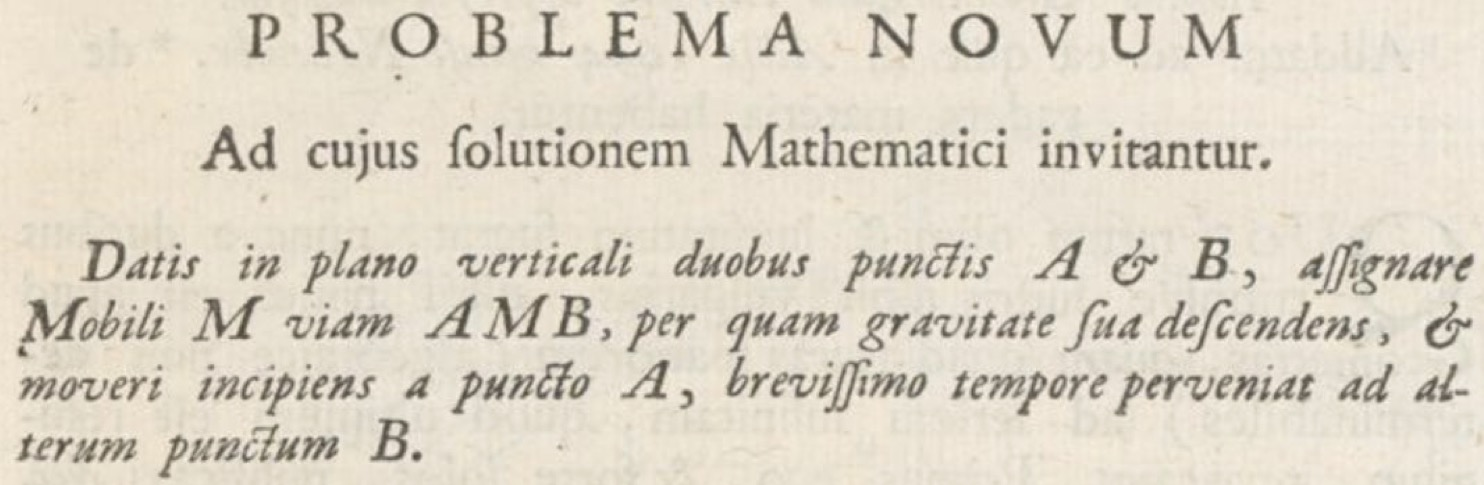
\includegraphics[width=0.8\textwidth]{chapters/020-variation/images/latein.jpg}
\end{center}
Zu deutsch:
\begin{quote}
Neue Aufgabe, zu deren Lösung die Mathematiker eingeladen werden.
Gegeben zwei Punkte $A$ und $B$ in einer vertikalen Ebene, finde
die Bahn $AMB$ eines Punktes $M$, der unter der Wirkung seines
Gewichtes in kürzester Zeit vom Punkt $A$ zum anderen Punkt $B$ absteigt.
\end{quote}
Die Situation der Aufgabenstellung ist in
Abbildung~\ref{buch:variation:fig:brachistochronenproblem}
dargestellt.
Bernoulli hat als Lösung gefunden, dass die Kurve eine Ausschnitt
aus einer Zykloide (in der Abbildung grau) sein muss.
Seine Lösung beruhte auf der Beobachtung, dass sich das Problem analog
zu einem Lichtausbreitungsproblem ist, für welches Fermat bereits
eine Lösung gefunden hat.

Da die Reibung vernachlässigt wird, ist die Energie des Massepunktes
erhalten.
Sie setzt sich aus der potenziellen und der kinetischen Energie
zusammen.
Die potenzielle Energie ist $-mgy$, die kinetische Energie ist
$\frac12mv^2$.
Die Energieerhaltung wird daher zu
\[
E=\frac12mv^2-mgy
\qquad\Rightarrow\qquad
v
=
\sqrt{2g}\!\sqrt{\frac{E}{gm}+y}
=
\!\sqrt{2(C+y)}.
\]
Durch Wahl einer anderen Zeiteinheit kann die Gleichung noch weiter
vereinfacht zu
\(
v = \sqrt{C+y}
\)
vereinfacht werden.
Gesucht ist also die zeitlich kürzeste Bahn eines Teilchens, 
dessen Geschwindigkeit auf bekannte Art $v(y)$ von der vertikalen
Koordinate abhängt.

%
% Das Fermat-Problem
%
\subsection{Das Fermat-Prinzip}
Bereits Fermat hat erkannt, dass das Brechnungsgesetz von Snellius
als Lösung eines Extremalproblems verstanden werden kann.

\begin{satz}[Fermat]
Sie $c/n_i$ die Geschwindigkeit, mit der sich Licht im Medium $M_i$
ausbreitet.
Ein Lichtstrahl von $A_1$ nach $A_2$ geht durch denjenigen Punkt $B$ 
auf der Grenzfläche zwischen den Medien, für den sich die Sinus der
Winkel $\alpha_i$ zwischen den Strahlen und der Normalen zur Grenzfläche
umgekehrt wie die $n_i$ verhalten, wenn also das Brechungsgesetz
\[
\frac{\sin\alpha_1}{\sin\alpha_2}
=
\frac{n_2}{n_1}
\]
gilt.
\end{satz}

\begin{proof}
Ohne der Beschränkung der Allgmeinheit können wir auf die Betrachtung
einer Ebene beschränken, die die beiden Punkte $A_i$ enthält und senkrecht
auf der Grenzfläche steht.
Wir dürfen weiter annehmen, dass die $x$-Achse in der Grenzfläche liegt 
und die Punkte $A_i$ die Koordinaten $(x_i,y_i)$ und der Punkt $B$ die
Koordinaten $(x,0)$ hat.
Es ist derjenige Punkt $x$ zu bestimmen, für den die Lichtzeit entlang 
des Pfades $A_1BA_2$ minimal wird.
Diese Zeit ist
\begin{align*}
t
&=
\frac{\overline{A_1B}}{c/n_1}
+
\frac{\overline{BA_2}}{c/n_2}
\\
ct
&=
n_1\overline{A_1B}
+
n_2\overline{A_2B}
\\
&=
n_1\!\sqrt{(x-x_1)^2 + y_1^2}
+
n_2\!\sqrt{(x_2-x)^2 + y_2^2}
\end{align*}
Das Minimum wird bei einer Nullstelle der Ableitung nach $x$ gefunden,
also bei einer Lösung der Gleichung
\begin{align*}
0
&=
n_1\frac{2(x_1-x)x}{\sqrt{(x_1-x)^2+y_1^2}}
+
n_2\frac{-2(x-x_2)x}{\sqrt{(x_2-x)^2+y_2^2}}.
\intertext{Indem man den zweiten Term auf der rechten Seite auf die linke
Seite bringt und durch $x$ dividiert, erhält man}
n_1
\frac{x_1-x}{\sqrt{(x_1-x)^2+y_1^2}}
&=
n_2
\frac{x-x_2}{\sqrt{(x_2-x)^2+y_2^2}}.
\end{align*}
Der Nenner ist auf beiden Seiten die Hypothenuse eines rechtwinkligen
Dreiecks, welches als Ankathete die Normale zur Grenzfläche hat.
Der Zähler ist die Gegenkathete des Winkels $\alpha_i$ zwischen der
Hypothenuse und der Normalen.
Daher ist der Quotient der Sinus des Winkels oder
\begin{equation}
n_1 \sin\alpha_1 = n_2 \sin\alpha_2.
\label{buch:variation:problem:eqn:snelliusinvariante}
\end{equation}
Die Gleichung~\eqref{buch:variation:problem:eqn:snelliusinvariante}
ist gleichbedeutend mit dem Brechungsgesetz
\[
\frac{\sin\alpha_1}{\sin\alpha_2}
=
\frac{n_2}{n_1}
\]
von Snellius.
\end{proof}

Der Satz von Fermat etabliert das Brechungsgsetz also Lösung eines
Extremalproblems.
Die Natur wählt für einen Lichtstrahl den zeitlich kürzesten Weg.
Der Beweis des Satzes von Fermat zeigt, dass entlang des Lichtstrahls
an jeder Grenzfläche zwischen Medien die Bedingung
\eqref{buch:variation:problem:eqn:snelliusinvariante}
erfüllt.
Wenn die optische Dichte $n$ eine Funktion von $n(y)$ ist, dann
wird der Lichtstrahl nicht nur in diskreten Punkten geknickt, sondern
entlang des ganzen Strahles gekrümmt.
Folgt der Strahl der Kurve $x(y)$, die mit der vertikalen den Winkel
$x'(y) = \tan\alpha(y)$ einschliesst.
Damit lässt sich auch die Sinus-Funktion ausdrücken, es gilt
\[
\sin\alpha(y)
=
\frac{x'(y)}{\pm\!\sqrt{x'(y)^2+1}}.
\]
Aus der Form~\eqref{buch:variation:problem:eqn:snelliusinvariante}
des Brechungsgesetztes wird dann die Gleichung
\begin{equation}
n_1\sin\alpha(y)
=
\frac{n_1(y)x'(y)}{\pm\!\sqrt{x'(y)^2+1}}
=
\operatorname{const}
\qquad\Rightarrow\qquad
\frac{n_1(y)^2x'(y)^2}{x'(y)^2+1}=C.
\label{buch:variation:eqn:fermatdgl}
\end{equation}
Dies ist eine Differentialgleichung für die Funktion $x(y)$.
Sie kann auch in die Form
\[
x'(y)^2
=
\frac{C}{(n_1(y)^2-C)}
\]
gebracht werden.

%
% Das Brachistochronenproblem als Lichtausbreitungsproblem
%
\subsubsection{Das Brachistochronenproblem als Lichtausbreitungsproblem}
Das Fermat-Prinzip besagt, dass ein Lichtstrahl, der sich in einem Medium
mit der Geschwindigkeit $c/n(y)$ ausbreitet, die Gleichung 
\eqref{buch:variation:eqn:fermatdgl} erfüllt.
Beim Brachistochronenproblem ist die Geschwindigkeit $v(y)=\!\sqrt{C-y}$ und 
damit $n(y) = c/\!\sqrt{C-y}$.
Eine Brachistochrone ist also eine Kurve, die die aus
\eqref{buch:variation:eqn:fermatdgl} folgende Gleichung
\begin{equation}
\frac{x'(y)^2}{(1+x'(y)^2)(C-y)} = K
\label{buch:variation:problem:eqn:bernoullidgl}
\end{equation}
erfüllen.

%
% Die Bernoullische Lösung
%
\subsubsection{Die Bernoullische Lösung}
Bernoulli hat gefunden, dass die Brachistochrone ein Zykloidenbogen ist.
Dies lässt sich dadurch verifizieren, dass man die Parametrisierung
einer Zykloide in die
Gleichung~\eqref{buch:variation:problem:eqn:bernoullidgl}
einsetzt.
Die Zykloide hat die Parametrisierung
\[
\left.
\begin{aligned}
x &= r(\varphi - \sin\varphi) 
\\
y &= r(1-\cos\varphi)
\end{aligned}
\right\}
\quad
\text{mit der Ableitung}
\quad
\left\{
\begin{aligned}
\dot{x}(\varphi) &= r(1-\cos\varphi)\\
\dot{y}(\varphi) &= r\sin\varphi
\end{aligned}
\right.
\]
für $\varphi\in\mathbb{R}$.
Die Ableitung ist
\[
x'(y)
=
\frac{\dot{x}(\varphi)}{\dot{y}(\varphi)}
=
\frac{1-\cos\varphi}{\sin\varphi}.
\]
Eingesetzt in \eqref{buch:variation:problem:eqn:bernoullidgl}
wird daraus
\[
\frac{\dot{x}(\varphi)^2}{
(\dot{y}(\varphi)^2 +\dot{x}(\varphi)^2)
(C-r(1-\cos\varphi))
}
=
\frac{(1-\cos\varphi)^2}{
((1-\cos\varphi)^2+\sin^2\varphi)
(C-r+r\cos\varphi)
}
=
K.
\]
Ausmultiplizieren im Nenner ergibt
\[
\frac{(1-\cos\varphi)^2}{
(1-2\cos\varphi+\cos^2\varphi+\sin^2\varphi)
(C-r+r\cos\varphi)
}
=
\frac{1-\cos\varphi}{
2(C-r+r\cos\varphi)
}
\]

%
% Das Brachistochronenproblem als Variationsproblem
%
\subsection{Das Brachistochronenproblem als Variationsproblem
\label{buch:variation:problem:subsection:variationsproblem}}
Die Bernoullische Lösung des Brachistochronenproblems verwendet die
Analogie zum Fermat-Prinzip.
Eine solche Analogie ist nur selten möglich, daher soll das Problem
jetzt in eine Form gebracht werden, in die auch viele ähnliche
Optimierungsproblem gebracht werden können.

Wir erinnern daran, dass die Geschwindigkeit des Massepunktes durch
$v(y)=\sqrt{C-y}$ gegeben ist.
Damit lässt sich die Zeit berechnen, die der Massepunkt entlang der
Lösungskurve braucht, wenn man diese als Funktion $y(x)$ mit beschreibt.
Die Punkte $A$ und $B$ sollen die $x$-Koordinaten $a$ bzw.~$b$ haben.
Für das Kurvenstück zwischen den $x$-Koordinaten $x$ und $x+\Delta x$
braucht der Massepunkt die Zeit
\[
\frac{ \sqrt{\Delta x^2 + \Delta y^2} }{v(y)}
=
\frac{ \sqrt{1 + y'(x)^2} }{ v(y) } \Delta x.
\]
Die Zeit ist das Integral
\begin{equation}
t
=
\int_a^b \frac{\sqrt{1+y'(x)^2}}{v(y(x))}\,dx
=
\int_a^b \sqrt{\frac{1+y'(x)^2}{C-y(x)}}\,dx.
\label{buch:variation:problem:eqn:brachint}
\end{equation}
Der Integrand auf der rechten Seite hängt nur von den Funktion $y(x)$
und $y'(x)$ ab.
Dies kommt vor allem daher, dass die Geschwindigkeit nur von $y$ abhängt,
nicht auch noch von $x$.
Im Allgemeinen wird man also davon ausgehen müssen, dass der Integrand
auch noch von $x$ abhängt.
Die Variationsrechnung befasst sich mit Problemen, in denen Funktionen
gefunden werden müssen, die ein Integral wie das in
\eqref{buch:variation:problem:eqn:brachint}
minimiert oder maximiert werden müssen.

\begin{definition}[Lagrange-Funktion des Brachistochronenproblems]
Die Lagrange-Funk\-tion des Brachistochronenproblems ist der
Integrand des Integrals
\eqref{buch:variation:problem:eqn:brachint},
\index{Lagrange-Funktion}%
also die Funktion
\[
L(x,y,y')
=
\sqrt{\frac{1+y^{\prime 2}}{C-y}}.
\]
\end{definition}

%
% Funktionale
%
\subsection{Funktionale
\label{buch:variation:problem:subsection:funktionale}}
Die Variationsrechnung löst Optimierungsproblem, die von einer
Funktion abhängen.
Um dies mathematisch präzis zu fassen, ist zunächst nötig, die Menge
der in Frage kommenden Funktionen so einzuschränken, dass die interessierende
Grösse überhaupt wohldefiniert ist.

%
% Vektorräume
%
\subsubsection{Vektorräume}
Zunächst sind die gemeinsamen algebraischen Eigenschaften zu charakterisieren,
die wir von den für unsere Untersuchungen zweckmässigen Funktionenmengen
erwarten.

\begin{definition}[Vektorraum]
Ein Vektorraum über den reellen Zahlen $\mathbb{R}$ ist einem Menge $V$ mit
zwei Operationen, der Addition und der Multiplikation mit Skalaren
\begin{align*}
    +\colon V\times V         &\to V : (u,v)\mapsto u+v
&
\cdot\colon \mathbb{R}\times V&\to V : (\lambda,v) \mapsto\lambda v
\end{align*}
mit den folgenden Eigenschaften.
\begin{enumerate}
\item
Es gelten die Assoziativgesetze
\begin{align*}
(u+v)+w&=u+(v+w)&&\text{für alle $u,v,w\in V$}\\
(\lambda \mu)v&=\lambda(\mu v)&&\text{für alle $\lambda,\mu\in\mathbb{R},\;v\in V$.}
\end{align*}
\item
Es gibt einen Vektor $0\in V$ mit der Eigenschaft $0+v=v$ für alle
Vektoren $v\in V$.
\item
Zu jedem Vektor $v\in V$ gibt es den entgegengesetzten Vektor $-v\in V$
mit der Eigenschaft, dass $-v+v=0$ ist.
\item
Die Addition von Vektoren ist kommutativ: $u+v=v+u$ für alle $u,v\in V$.
\item
Es gelten die Distributivgesetze 
\begin{align*}
(\lambda + \mu) v &= \lambda v + \mu v
	&\quad\text{für alle $\lambda,\mu\in\mathbb{R},\;v\in V$}\\
\lambda(u+v)      &= \lambda u + \lambda v
	&\quad\text{für alle $\lambda\in\mathbb{R},\;u,v\in V$}
\end{align*}
\end{enumerate}
\end{definition}

Die Mengen $\mathbb{R}^n$ erfüllen die genannten Eigenschaften, sind
also Vektorräume.
Die Definition eines Vektorraums ist aber viel allgemeiner, insbesondere
gehören dazu auch Mengen von Funktionen.
Damit wird es möglich, die Berechnungen in $\mathbb{R}^n$ auf Funktionen
auszudehnen.
Zum Beispiel bilden die stetigen Funktionen auf einem Intervall einen
Vektorraum, wie das folgende Beispiel zeigt.

\begin{beispiel}
Die Menge
\[
C([a,b])
=
\{f\colon[a,b]\to\mathbb{R}\mid \text{$f$ ist stetig}\}
\]
der stetigen Funktionen bildet einen Vektorraum.
Die Operationen sind die punktweise Addition von Funktionen und die
Multiplikation der Werte mit Skalaren, für $f,g\in C([a,b])$ und
$\lambda\in \mathbb{R}$ ist
\begin{align*}
(f+g)(x) &= f(x)+g(x)
&&\text{und}&
(\lambda f)(x) &= \lambda f(x).
\end{align*}
Entscheidend ist, dass die Addition von Funktionen und die Multiplikation
mit Skalaren nicht aus der Menge herausführt.
Tatsächlich wird in der Analysis gezeigt, dass die Summe stetiger Funktionen
wieder stetig ist und dass die Funktion $x\mapsto \lambda f(x)$ stetig,
wenn $f$ stetig ist.
Die übrigen Eigenschaften sind ebenfalls erfüllt, da sie bereits für die
Funktionswerte erfüllt sind.
\end{beispiel}

%
% Norm und Grenzwerte
%
\subsubsection{Norm und Grenzwerte}
Um Analysis zu betreiben, muss man ausdrücken können, dass eine Folge
von Funktionen konvergiert.
Dazu ist ein Abstandsbegriff zwischen Funktionen nötig.

\begin{definition}[Norm, normierter Raum]
Eine {\em Norm} auf einem Vektorraum $V$ ist eine Abbildung
\index{Norm}%
$\|\cdot\|\colon V\to\mathbb{R}^+_0$ mit nichtnegativen reellen Werten
und den folgenden Eigenschaften
\begin{itemize}
\item Definitheit: $\|v\|\ge 0$ für $v\in V$ mit Gleichheit 
genau dann, wenn $v=0$.
\index{Definitheit}%
\item Absolute Homogenität: Für alle Vektoren $v\in V$ und
\index{Homogenität}%
$\lambda\in\mathbb{R}$ gilt $\|\lambda v\| = |\lambda|\, \|v\|$.
\item Dreiecksungleichung: für alle Vektoren $u,v\in V$ gilt
\index{Dreiecksungleichung}%
$\|u+v\|\le \|u\|+\|v\|$.
\end{itemize}
Ein {\em normierter Raum} ist ein Vektorraum mit einer Norm.
\index{normierter Raum}%
\end{definition}

\begin{beispiel}
Der Vektorraum der stetigen Funktionen kann mit der Supremum-Norm
\[
\|f\| = \sup_{x\in[a,b]} |f(x)|
\]
zu einem normierten Raum gemacht werden.
Die Definitheit ist durch die Definition offensichtlich sichersgtellt.
Für $\|\lambda f\|$ finden wir
\[
\|\lambda f\|
=
\sup_{x\in[a,b]} |\lambda f(x)|
=
|\lambda|\,
\sup_{x\in[a,b]} |f(x)|
=
|\lambda|\, \|f\|,
\]
was die Homogenität zeigt.
Die Dreiecksungleichung folgt aus
\begin{align*}
\|f+g\|
&=
\sup_{x\in[a,b]} |f(x)+g(x)|
\\
&\le
\sup_{x\in[a,b]} (|f(x)|+|g(x)|)
\\
&\le
\sup_{x\in[a,b], y\in[a,b]} (|f(x)|+|g(y)|)
\\
&=
\sup_{x\in[a,b]} |f(x)|
+
\sup_{y\in[a,b]} |g(y)|
=
\|f\| + \|g\|.
\qedhere
\end{align*}
\end{beispiel}

Mit einer Norm ist es jetzt möglich, die Konvergenz von Folgen und den
Begriff des Grenzwertes zu definieren.

\begin{definition}[Cauchy-Folge, Grenzwert]
Eine Folge $(x_n)_{n\in\mathbb{N}}$ in $V$ in einem normierten Raum $V$
mit der Norm $\|\cdot\|$
heisst eine Cauchy-Folge, wenn es für jedes $\varepsilon>0$ eine
\index{Cauchy-Folge}%
$N\in \mathbb{N}$ gibt derart, dass
\[
\| x_n - x_m \| < \varepsilon
\quad\forall n,m\ge N.
\]
Der Vektor $x\in V$ heisst {\em Grenzwert} der Folge $(x_n)_{n\in\mathbb{N}}$,
\index{Grenzwert}%
wenn es zu jedem $\varepsilon > 0$ ein $N\mathbb{N}$ gibt derart, dass
\[
\|x_n-x\| < \varepsilon 
\quad\forall n\ge N.
\]
Die Folge $(x_n)_{n\in\mathbb{N}}$  in $V$ heisst {\em konvergent}, wenn
\index{konvergent}%
$x$ der Grenzwert von $(x_n)_{n\in\mathbb{N}}$ ist.
\end{definition}

Der durch die Supremum-Norm definierte Konvergenzbegriff ist die gleichmässige
Konvergenz.
Zur Erinnerung:
Eine Folge $f_n$ von Funktionen heisst gleichmässig konvergent gegen die
Funktion $f$, wenn es zu jedem
$\varepsilon >0$ ein $N\in\mathbb{N}$ gibt derart, dass
\[
|f_n(x) - f(x)|<\varepsilon\quad\forall n>N\text{ und }x\in [a,b].
\]
Die Supremum-Norm ist
\[
\|f_n(x) - f(x)\|
=
\sup_{x\in[a,b]} |f_n(x)-f(x)| < \varepsilon
\]
für alle $n>N$.
Dies ist genau die Konvergenz in der Norm $\|\cdot\|$.
Aus der Analysis ist bekannt, dass eine gleichmässig konvergente 
Funktionenfolge gegen eine stetige Funktion konvergiert.

\begin{definition}[Banach-Raum]
Ein normierter Raum $V$ heisst ein {\em Banach-Raum},
\index{Banach-Raum}%
wenn jede Cauchy-Folge in $V$ einen Grenzwert hat.
\end{definition}

\begin{beispiel}
Die Menge $C^1([0,2])$
der stetigen Funktionen auf dem Intervall $[0,2]$ ist ein normierter
Raum mit der Norm
\[
\|f\|_1
=
\int_0^2 |f(x)|\,dx,
\]
die auch die $L^1$-Norm heisst.
\index{L1-Norm@$L^1$-Norm}%
Zunächst ist nachzuprüfen, dass dies tatsächlich eine Norm ist.
Die Definitheit und die Homogenität von $\|\cdot\|_1$ ist klar, nur
die Dreiecksungleichung erfordert etwas Arbeit.
Für Funktionen $f,g\in L^1([0,2])$ gilt
\begin{align*}
\|f+g\|_1
&=
\int_0^2 |f(x)+g(x)|\,dx
\\
&\le 
\int_0^2 |f(x)|+|g(x)|\,dx
=
\int_0^2 |f(x)|\,dx
+
\int_0^2 |g(x)|\,dx
=
\|f\|_1+\|g\|_1,
\end{align*}
was die Dreeicksungleichung beweist.

Eine Cauchy-Folge in der $L^1$-Norm muss aber nicht unbedingt einen
stetigen Grenzwert haben.
Die Funktionen
\(
f_n(x) =
\begin{cases}
x^n&\quad x< 1\\
1&\quad x\ge 1
\end{cases}
\)
haben die $L^1$-Norm
\begin{align*}
\|f_n-f_m\|_1
=
\int_0^2 |f_n(x)-f_m|\,dx
\\
&=
\biggl|\int_0^1 x^n-x^m\,dx\biggr|
=
\biggl[
\biggl|
\frac{1}{n+1}x^{n+1}
-
\frac{1}{m+1}x^{m+1}
\biggr|
\biggr]_0^1
\\
&=
\biggl|
\frac{1}{n+1}
-
\frac{1}{m+1}\biggr|.
\end{align*}
Wegen
\[
\|f_n-f_m\|_1
<\varepsilon
\]
für $n,m>2/\varepsilon$ ist $f_n$ eine Cauchy-Folge in $L^1$.
In $L^1$ konvergiert die Folge $f_n$ gegen die Funktion
\[
f(x)
=
\begin{cases}
0&\quad x< 1\\
1&\quad x\ge 1.
\end{cases}
\]
Diese Funktion ist aber nicht stetig, da sie bei $x=1$ einen
Sprung hat.
Bezüglich der $L^1$-Norm ist $C^1([a,b])$ als im Allgemeinen
kein Banach-Raum.
\end{beispiel}

%
% Stetige und differenzierbare Funktionen
%
\subsubsection{Stetige und differenzierbare Funktionen}
Mit der Norm lässt sich auch die Stetigkeit von Abbildungen zwischen
normierten Räumen definieren.

\begin{definition}[Stetigkeit]
Eine Funktion $f\colon U\to V$ zwischen normierten Räumen heisst
{\em stetig im Punkt} $x\in U$, wenn es zu jedem $\varepsilon > 0$
\index{stetig in einem Punkt}%
ein $\delta > 0$
gibt derart, dass
\(
\|f(x)-f(y)\| < \delta
\)
wenn
\(
\|x-y\|<\varepsilon
\).
Eine Funktion $f\colon U\to V$ heisst {\em stetig}, wenn sie in
jedem Punkt von $U$ stetig ist.
\end{definition}

Das Bild einer Folge $x_n\in U$, die gegen $x_0\in U$ konvergiert,
ist eine Folge $f(x_n)$ in $V$.
Man sagt, $y\in V$ sei der Grenzwert von $f(x)$ für $x\to x_0$,
wenn $f(x_n)$ für jede solche Folge $x_n$ gegen $y$ konvergiert.
Der Grenzwert wird auch
\[
\lim_{x\to x_0} f(x)
=
y
\]
geschrieben.
Stetige Funktionen zeichnen sich wie in der Analysis der Funktionen
einer Variablen dadurch aus, dass der Grenzwert der Werte der Funktion
auf einer konvergenten Folge mit dem Funktionswert des Grenzwertes
übereinstimmt.

\begin{satz}
Eine Funktion $f\colon U\to V$ ist genau dann stetig im Punkt $x\in U$,
wenn für jede Folge $x_n$ in $U$ mit Grenzwert $x$ die Folge $f(x_n)$
konvergent ist und
\[
\lim_{n\to\infty} f(x_n) = f(x).
\]
Eine lineare Funktion $f\colon U\to V$ ist genau dann stetig,
wenn für jede Nullfolge $x_n$ in $U$ 
\[
\lim_{n\to \infty} f(x_n) = 0
\]
gilt.
\end{satz}

\begin{definition}
Eine Funktion $f\colon U\to V$ zwischen normierten Räumen heisst
differenzierbar im Punkt $x\in U$ wenn es eine lineare Funktion
$Df(x_0)\colon U\to V$ gibt derart, dass
\[
f(x+v) =f(x) + Df(x_0)\cdot v + o(v),
\]
wobei $o(v)$ bedeutet, dass für diese Funktion
\[
\frac{o(v)}{|v|}\to 0
\quad\text{für $v\to 0$}
\]
gilt.
\end{definition}

Funktionen auf einem Vektorraum mit reellen Werten weren auch
{\em Funktionale} genannt.
\index{Funktional}
Vor dem 20.~Jahrhundert wurde häufig ein Untersschied zwischen
Funktionen von endlich vielen reellen Variablen und Funktionen
von einem unendlichdimensionalen Vektorraum gemacht.
Die Entwicklungen dieses  Abschnittes haben gezeigt, dass eine
solche Unterscheidung nicht gerechtfertigt ist.
Es ist lediglich notwendig, die Definitionen allgemein genug zu
fassen und sich jederzeit über die Funktionenmenge und die zu
verwendende Norm Rechenschaft abzulegen.


%
% 2-fundamtenallemma.tex
%
% (c) 2023 Prof Dr Andreas Müller
%
\section{Das Fundamentallemma
\label{buch:variation:section:fundamentallemma}}
\kopfrechts{Das Fundamentallemma}
Im Fall des endlichdimensionalen Extremalproblems ist aus der
Forderung, dass alle Richtungsableitung verschwinden müssen, 
die Bedingung geworden, dass
\[
v\cdot\grad f = 0
\]
sein muss für alle Vektoren $v\in\mathbb{R}^n$.
Wir haben daraus geschlossen, dass der Gradient $\grad f=0$
sein muss.
Wir hatten dies das endlichdimensionale Fundamentallemma genannt,
wegen $e_k\cdot \grad f = D_kf$ war es eine ziemliche Selbstverständlichkeit.
Bei der Lösung von Variationsproblemen, wo es nicht um endlichdimensionale
Vektoren und das Skalarprodukt, sondern um Funktionen und Integrale
geht, brauchen wir eine ähnliche Aussage für Funktionen.

%
% Positive glatte Funktionen mit kompaktem Träger
%
\subsection{Positive glatte Funktionen mit kompaktem Träger}
Die Aussage des Fundamentallemmas für endlichdimensionale Vektoren 
folgte sofort aus der Tatsache, dass es für jedes $k$ einen Vektor
$e_k$ gibt, der nur in der Koordinaten $k$ von $0$ verschieden ist.
Natürlich gibt es auch Funktionen, die nur in genau einem Punkt
von $0$ verschieden sind.
Eine solche Funktion ist aber im allgemeinen nicht differenzier-
oder integrierbar.
In diesem Abschnitt soll daher gezeigt werden, dass es unendlich
oft stetig differnzierbare Funktionen gibt, die nur in einem beliebig
kleinen vorgegebenen Intervall $\ge 0$ sind.

\begin{definition}[Träger]
Der {\em Träger} einer Funktion $f\colon X\to\mathbb{R}$ ist die Menge
\index{Träger}%
\[
\supp f = \{ x\in X\mid f(x)\ne \}.
\]
\end{definition}

Gesucht ist also eine beliebig oft stetig differenzierbare Funktion,
deren Träger in einem vorgegebenen Intervall $[a,b]$ enthalten ist.
Wir konstruieren so eine Funktion in zwei Schritten.

\input{chapters/020-variation/fig/f.tex}

\begin{satz}
\label{buch:variation:fundamentallemma:satz:glatt}
Die Funktion
\[
f(x)
=
\begin{cases}
e^{-1/x}&\qquad x>0\\
0&\qquad x\le 0
\end{cases}
\]
(siehe auch Abbildung~\ref{buch:variation:fundamentallemma:fig:glatt})
ist beliebig oft stetig differenzierbar.
\end{satz}

\begin{proof}
Es ist klar, dass die Funktion $f$ beliebig oft stetig differenzierbar
ist in jedem Punkt $x\ne 0$.
Es ist also nur nachzuweisen, dass $f(x)$ im Punkt $0$ beliebig
oft stetig differenzierbar ist.

Die ersten drei Ableitungen von $f(x)$ sind
\begin{align}
f'(x) &= \frac{1}{x^2} f(x)
\label{buch:variation:fundamentallemma:eqn:f1}
\\
f''(x) &= \frac{1-2x}{x^4}f(x)
\notag
\\
f'''(x) &= \frac{6x^2-6x+1}{x^6}f(x).
\notag
\end{align}
Daraus lässt sich die Vermutung ableiten, dass
\begin{equation}
f^{(n)}(x)
=
\frac{p_{n-1}(x)}{x^{2n}} f(x)
\label{buch:variation:fundamentallemma:eqn:fabl}
\end{equation}
ist, wobei $p_k(x)$ ein Polynom vom Grad $k$ ist.
Wir beweisen diese Vermutung mit Hilfe von vollständiger Induktion.
Die Induktionsverankerung für die $0$-te Ableitung ist trivial.

Wir nehmen jetzt im Sinne der Induktionsannahme an, dass die $n$-te
Ableitung die Form \eqref{buch:variation:fundamentallemma:eqn:fabl}
hat.
Wir müssen zeigen, dass dann auch $f^{(n+1)}(x)$ diese Form hat.
Dazu berechnen wir
\begin{align}
f^{(n+1)}(x)
&=
\frac{d}{dx}
\frac{p_n(x)}{x^{2n}} f(x)
\notag
\\
&=
\frac{p_n'(x)}{x^{2n}} f(x)
-2n
\frac{p_n(x)}{x^{2n+1}} f(x)
+
\frac{p_n(x)}{x^{2n}} f'(x).
\notag
\intertext{Mit der ersten Ableitung
\eqref{buch:variation:fundamentallemma:eqn:f1} wird dies zu}
&=
\frac{p_n'(x)}{x^{2n}} f(x)
-2n
\frac{p_n(x)}{x^{2n+1}} f(x)
+
\frac{p_n(x)}{x^{2n}} \frac{1}{x^2}f(x)
\notag
\\
&=
\frac{x^2p_n'(x) -2nxp_n(x)+p_n(x)}{x^{2n+2}} f(x).
\label{buch:variation:fundamentallemma:eqn:induktionsschritt}
\end{align}
Die Ableitung $p_n'(x)$ ist ein Polynom vom Grad $n-1$ und damit
ist $x^2p_n'(x)$ ein Polynom vom Grad $n+1$.
Ebenso ist $xp_n(x)$ ein Polynom vom Grad $n+1$ während
$p_n(x)$ ein Polynom vom Grad $n$ ist.
Der Zähler von
\eqref{buch:variation:fundamentallemma:eqn:induktionsschritt}
ist
\[
p_{n+1}(x)
=
x^2p_n'(x)+(1 -2nx)p_n(x),
\]
ein Polynom vom Grad $n+1$.
Damit ist der Induktionsschritt erfolgreich und die Behauptung betreffend
die Form von $f^{(n)}(x)$ ist bewiesen.

Es ist jetzt nur noch zu zeigen, dass der Grenzwert von $f^{(n)}(x)$
für $x\to 0+$ verschwindet.
Da das Polynom $p_n(x)$ stetig ist, folgt
\[
\lim_{x\to 0}
f^{(n)}(x)
=
\lim_{x\to 0}\frac{p_n(x)}{x^{2n}}f(x)
=
p_n(0) \lim_{t\to\infty} t^{2n} e^{-t}
=
0.
\]
Damit ist die beliebige stetige Differenzierbarkeit an der Stelle
$x=0$ gezeigt.
\end{proof}

Die Funktion $f(x)$ von 
Satz~\ref{buch:variation:fundamentallemma:satz:glatt} 
erfüllt noch nicht die Forderung, dass sie nur in einem vorgegebenen
Intervall von $0$ verschieden ist.

\input{chapters/020-variation/fig/g.tex}

\begin{satz}
\label{buch:variation:fundamentallemma:satz:gab}
Sei $f(x)$ die Funktion von
Satz~\ref{buch:variation:fundamentallemma:satz:glatt}.
Dann ist
\[
g_{a,b}(x)
=
f(x-a) f(b-x)
\]
eine unendlich oft stetig differenzierbare, nichtnegative Funktion mit Träger
$\supp g_{a,b}=(a,b)$.
\end{satz}

Die Funktionen $g_{a,b}(x)$ sind beliebig oft differenzierbar und nur im
Intervall $[a,b]$ von $0$ verschieden und sogar positiv.
Weil sie stetig sind, sind sie auch integrierbar, man kann also das
Integral über $\mathbb{R}$ berechnen und die Funktion damit normieren.
Die neue Funktion
\[
\frac{1}{N}
\tilde{g}_{a,b}(x)
\qquad\text{mit}\;
N
=
\int_{-\infty}^{\infty}g_{a,b}(x)\,dx
=
\int_a^b g_{a,b}(x)\,dx
\]
ist immer noch beliebig oft stetig differenzierbar und hat zusätzlich die
Eigenschaft
\[
\int_{-\infty}^{\infty}
\tilde{g}_{a,b}(x)\,dx
=
\int_a^b
\tilde{g}_{a,b}(x)\,dx
=
1.
\]
Wir formulieren dieses Resultat als Satz.

\begin{satz}
\label{buch:variation:satz:gabeins}
Zu jedem Intervall $[a,b]$ gibt es eine beliebig oft stetig
differenzierbare Funktion $g(x)$, genau das Intervall $[a,b]$
als Träger hat und deren Integral über $[a,b]$ den Wert $1$ hat.
\end{satz}

%
% Das Fundamentallemma
%
\subsection{Das Fundamentallemma}
Mit der Funktion $g_{a,b}(x)$ von
Satz~\ref{buch:variation:fundamentallemma:satz:gab}
lässt sich jetzt das Fundamentallemma in der folgenden Form
leicht beweisen.

\begin{satz}[Fundamentallemma]
\label{buch:variation:fundamentallemma:satz:fundamentallemma}
Wenn für die stetige Funktion $f\colon[a,b]\to\mathbb{R}$ 
\begin{equation}
\int_a^b f(x)\varphi(x)\,dx = 0
\label{buch:variation:fundamentallemma:eqn:fundamentalbed}
\end{equation}
gilt für jede beliebig oft stetig differenzierbare Funktion $\varphi(x)$ 
dann ist $f(x)=0$.
Das Resultat gilt selbst dann, wenn
\eqref{buch:variation:fundamentallemma:eqn:fundamentalbed}
nur für beliebig oft stetig differenzierbare Funktionen $\varphi(x)$ 
gilt, die ausserdem an den Intervallenden verschwinden:
$\varphi(a)=\varphi(b)=0$.
\end{satz}

\begin{proof}
Wir zeigen mit Hilfe eines Widerspruchs, dass es keinen Punkt $x_0\in[a,b]$
geben kann, für den $f(x_0)\ne 0$ ist.
Dazu nehmen wir also an, dass $f(x_0)\ne 0$ ist.
Falls $f(x_0)<0$ ist, ersetzen wir $f$ durch $-f$, 
die Bedingung
\eqref{buch:variation:fundamentallemma:eqn:fundamentalbed}
ändert sich dadurch nicht.
\input{chapters/020-variation/fig/fundamentallemma.tex}
Wir dürfen daher annehmen, dass $f(x_0)>0$ ist
(Abbildung~\ref{buch:variation:fundamentallemma:fig:beweis}).
Da $f$ stetig ist, gibt es ein Intervall $[x_0-\varepsilon,x_0+\varepsilon]$
derart, dass $f(x)> \frac12 f(x_0)$ für
$x\in[x_0-\varepsilon,x_0+\varepsilon]$ gilt.
Dann gilt für das Integral
\[
\int_a^b
f(x)
g_{x_0-\varepsilon,x_0+\varepsilon} (x)
\,dx
>
\frac{f(x_0)}{2}
\int_a^b
g_{x_0-\varepsilon,x_0+\varepsilon} (x)
\,dx
>
0
\]
im Widerspruch zur Bedingung
\eqref{buch:variation:fundamentallemma:eqn:fundamentalbed}.
Der Widerspruch zeigt, dass $f(x)=0$ sein muss.
\end{proof}

%
% Skalarproduktformulierung des Fundamentallemmas
%
\subsection{Skalaproduktformulierung des Fundamentallemmas}
Die Richtungsableitung einer Funktion endlich vieler Variablen 
konnte als Skalarprodukt mit dem Gradienten geschrieben werden und
das Fundamentallemma hat besagt, dass der Gradient verschwindet,
wenn alle Richtungsableitungen verschwinden.
Diese Schlussweise ist auch für Funktionen möglich, wenn man Funktionen
ein Skalarprodukt definieren kann.

\begin{definition}[$L^2$-Skalarprodukt]
Das {\em Skalarprodukt} zweier quadratintegrierbarer Funktion $f$ und $g$
auf dem Intervall $[a,b]$ ist definiert durch
\[
\langle f,g\rangle
=
\int_a^b f(x)g(x)\,dx.
\]
\end{definition}

\begin{satz}[Fundamentallemma, Skalarproduktform]
Wenn für eine stetige Funktion $f\colon[a,b]\to\mathbb{R}$ das Skalarprodukt
\[
\langle f,\varphi\rangle = 0
\]
ist für jede unendlich oft differenzierbare Funktion $\varphi$ auf dem
Intervall $[a,b]$, dann ist $f=0$.
\end{satz}



%
% 3-eulerlagrange.tex
%
% (c) 2023 Prof Dr Andreas Müller
%
\section{Die Euler-Lagrange Differentialgleichung
\label{buch:variation:section:eulerlagrange}}
\kopfrechts{Die Euler-Lagrange Differentialgleichung}
Das Neuartige an der Aufgabenstellung des Brachistochronenproblems
war, dass eine Funktion gesucht war, so dass ein damit gebildetes
Integral eine Minimaleigenschaft erfüllt.
Für die damalige Mathematik war die Aufgabe, eine Funktion zu finden,
nicht neu.
Die Theorie der Differentialgleichungen war bereits entwickelt,
Newton hat die Infinitesimalrechnung ja erfunden, um damit die
Bewegungsgleichungen der Physik zu formulieren und zu lösen.
In einer Differentialgleichung werden Werte und Ableitungen einer
Funktion an einer einzigen Stelle miteinander verbunden.
Etwas salop formuliert sagt die Differentialgleichung in jedem
Punkt, in welche Richtung und mit welcher Krümmung die Funktionskurve
weiter zu zeichnen ist.

Im Brachistochronenproblem tragen aber alle Werte der gesuchten
Funktion zum Integral bei, es scheint daher auf den ersten Blick
nicht möglich, das Problem durch schrittweise Konstruktion
``von Punkt zu Punkt'' der Lösungskurve zu konstruieren.

Bernoullis Lösung des Brachistochrononproblems beruht auf der
Beobachtung, dass sich die Bedinung für die schnellste Bahn
durch eine Bedingung ersetzen lässt, die in jedem einzelnen
Punkt ausgewertet werden kann.
Das von ihm verwendete Fermat-Prinzip wurde ursprünglich ebenfalls
als eine globale Eigenschaft eines Lichtstrahls formuliert.
Aus dem Fermat-Prinzip folgt aber das Brechungsgesetz, welches
sagt, dass die Richtung eines Strahls in einem Punkt genau dann
ändert, wenn sich dort auch der Brechungsindex der beiden Medien
ändert.
Das Fermat-Prinzip ist also ein Beispiel dafür, wie eine globale
Bedingung erfüllt werden kann, indem einer lokalen Regel in jedem
Punkt gefolgt wird.

Es ist das Verdienst von Euler und Lagrange, zu erkennen, dass diese
Übersetzung eines globalen Variationsproblems in ein lokales 
Problem immer möglich ist.
Es entsteht dabei die Euler-Lagrange-Differentialgleichung, welche
die Problemstellung auf die Lösung einer Differentialgleichung
reduziert.
Damit ist ein allgemein anwendbares Lösungsverfahren gefunden.
Zu einem Variationsproblem lässt sich immer eine Differentialgleichung
finden, welche die gesuchte Funktion als Lösung hat.

In diesem Abschnitt soll dieser indirekte Weg der Lösung von
Variationsaufgaben dargestellt werden.
Wir werden später zeigen, dass diese Vorgehensweise nicht immer
erfolgreich sein kann.
Zum Beispiel werden wir in Kapitel~\ref{buch:chapter:nichtdiff}
Variationsprobleme kennenlernen, deren Lösungskurven nicht
differenzierbar sind und daher auch nicht von einer Differentialgleichung
gefunden werden können.
Im Kapitel~\ref{buch:chapter:direkt} werden daher die sogenannten
direkten Methodn vorgestellt, die den Umweg über eine
Differentialgleichung vermeiden.

%
% Die Lagrange-Funktion
%
\subsection{Die Lagrange-Funktion
\label{buch:variation:eulerlagrange:subsection:lagrange-funktion}}
Wir betrachten Variationsproblem der folgenden Art.
Gesucht ist eine auf dem Intervall $[x_0,x_1]$ definirte
Funktion $y(x)$, die das Integral
\begin{equation}
I(y)
=
\int_{x_0}^{x_1}
F(x, y(x), y'(x))
\,dx
\label{buch:variation:eulerlagrange:eqn:funktional}
\end{equation}
maximiert oder minimiert.
Der Ausdruck~\eqref{buch:variation:eulerlagrange:eqn:funktional}
wird ein Funktional genannt.
Die Funktion
\[
F
\colon
\mathbb{R}\times
\mathbb{R}\times
\mathbb{R}
\to
\mathbb{R}
\]
von drei Variablen heisst die {\em Lagrange-Funktion}
des Funktionals \eqref{buch:variation:eulerlagrange:eqn:funktional}.

\begin{beispiel}
Die Lagrange-Funktion des Brachistochronenproblems ist
\[
F(x,y,y')
=
\sqrt{ \frac{1+y^{\prime 2}}{y} }.
\]
Die Funktion hängt nicht von $x$ ab, was bedeutet, dass eine
Verschiebung in $x$-Richtung die Form der Lösungsfunktion des
Variationsproblems nicht ändert.
\end{beispiel}

\begin{beispiel}
\label{buch:variation:eulerlagrange:beispiel:gerade}
Wir formulieren die Aufgabe, die kürzeste Verbindung der Punkte
$(x_0,y_0)$ und $(x_1,y_1)$ in einer Ebene zu finden, als Variationsproblem.
Die Länge einer Kurve $y(x)$ ist das Integral
\[
l(y)
=
\int_{x_0}^{x_1}
\sqrt{1+y'(x)^2}\,dx.
\]
Daraus lesen wir ab, dass die Lagrange-Funktion dieses Variationsproblems
\begin{equation}
F(x,y,y') = \sqrt{1+y^{\prime 2}}
\label{buch:variation:eulerlagrange:eqn:geradeL}
\end{equation}
ist.
Die Funktion hängt weder von $x$ noch von $y$ ab.
Dies ist auch zu erwarten, denn die Länge einer Kurve hängt nicht davon
ob, wo in der Ebene sie platziert ist.
Eine Verschiebung in $x$-Richtung würde das $x$-Argument ändern,
eine Verschiebung in $y$-Richtung die $y$-Werte.
Wäre $F$ von $x$ oder $y$ abhängig, könnte auch die Länge der Kurve
davon abhängen.
\end{beispiel}

%
% Euler-Lagrange_Differentialgleichung
%
\subsection{Euler-Lagrange-Differentialgleichung
\label{buch:variation:eulerlagrange:subsection:dgl}}
\input{chapters/020-variation/fig/variation0.tex}
Das Maximum oder Minimum einer Funktionen mehrere Variablen wurde
gefunden, indem die Richtungsableitung berechnet und $=0$ gesetzt
wurde.
Um die Funktion zu bestimmen, die ein Funktional $I(y)$ zu einem
Maximum oder Minimum macht, versuchen wir, die Idee der Richtungsableitung
für ein Funktional nachzuahmen.
Wir nehmen daher an, dass $y(x)$ eine Funktion ist, die das Funktional
$I(y)$ zu einem Minimum macht.
Für die Richtungsableitung addieren wir ein Vielfaches einer
Funktion $\eta(x)$, die Summe $y(x)+\varepsilon\eta(x)$ entspricht
dann einer Geraden mit Richtung $\eta(x)$ im Funktionenraum
(Abbildung~\ref{buch:variation:fig:variation0}).
Die Funktionen $y(x)+\varepsilon\eta(x)$ sind aber nur dann Kandidaten
für eine Lösung des Problems, wenn immer noch
\begin{align*}
y(x_0) + \varepsilon \eta(x_0) &= y_0
&&\text{und}&
y(x_1) + \varepsilon \eta(x_1) &= y_1
\end{align*}
gilt.
Dies ist nur möglich, wenn $\eta(x_0)=\eta(x_1)=0$ ist.

Wir berechnen jetzt die Ableitung der Funktion
$\varepsilon\mapsto I(y+\varepsilon\eta )$ an der Stelle $\varepsilon=0$.
Da die Intervallgrenzen nicht von $\varepsilon$ abhängen, können wir
die Ableitung unter das Integral nehmen:
\begin{align*}
\frac{d}{d\varepsilon}
I(y+\varepsilon\eta)
&=
\int_{x_0}^{x_1}
\frac{d}{d\varepsilon}
F(x,y(x)+\varepsilon\eta(x),y(x)+\varepsilon\eta'(x))
\,dx.
\intertext{Da $F$ differenzierbar ist, kann die Ableitung mit der
Kettenregel berechnet werden, sie ist}
&=
\int_{x_0}^{x_1}
\frac{\partial F}{\partial y}
(x,y(x)+\varepsilon\eta(x),y(x)+\varepsilon\eta'(x))
\eta(x)
\\
&\qquad
+
\frac{\partial F}{\partial y'}
(x,y(x)+\varepsilon\eta(x),y(x)+\varepsilon\eta'(x))
\eta'(x)
\,dx.
\intertext{Uns interessiert aber nur der Wert an der Stelle $\varepsilon=0$,
er ist}
\frac{d}{d\varepsilon}
I(y+\varepsilon\eta)
\bigg|_{\varepsilon=0}
&=
\int_{x_0}^{x_1}
\frac{\partial F}{\partial y}
(x,y(x),y'(x))
\,
\eta(x)
+
\frac{\partial F}{\partial y'}
(x,y(x),y'(x))
\,
\eta'(x)
\,dx
=0.
\end{align*}
Das Integral hängt von den verschiedenen Faktoren $\eta(x)$ und
von $\eta'(x)$ in den beiden Termen unter dem Integral ab.
Wir integrieren den zweiten Term partiell 
\begin{align*}
\int_{x_0}^{x_1}
\frac{\partial F}{\partial y'}(x,y(x),y'(x))\,\eta'(x)\,dx
&=
\biggl[
\frac{\partial F}{\partial y'}(x,y(x),y'(x))\,\eta(x)
\biggr]_{x_0}^{x_1}
\\
&\qquad
-
\int_{x_0}^{x_1}
\frac{d}{dx}
\frac{\partial F}{\partial y'}(x,y(x),y'(x))\,\eta(x)\,dx.
\end{align*}
Da $\eta(x_0)=\eta(x_1)=0$ verschwindet der erste Term
auf der rechten Seite, es bleibt
\[
\frac{d}{d\varepsilon}
I(y+\varepsilon\eta)
\bigg|_{\varepsilon=0}
=
\int_{x_0}^{x_1}
\biggl(
\frac{\partial F}{\partial y}
(x,y(x),y'(x))
-
\frac{d}{dx}
\frac{\partial F}{\partial y'}
(x,y(x),y'(x))
\biggr)
\eta(x)
\,dx.
\]
Dies kann auch als Skalarprodukt
\[
\biggl\langle 
\frac{\partial F}{\partial y}
(x,y(x),y'(x))
-
\frac{d}{dx}
\frac{\partial F}{\partial y'}
(x,y(x),y'(x))
,
\eta(x)
\biggr\rangle
=
0
\]
geschrieben werden.
Da dies für jede differenzierbare Funktion $\eta$ mit Randwerten
$\eta(x_0)=\eta(x_1)$ gelten muss, folgt nach dem
Fundamentallemma~\ref{buch:variation:fundamentallemma:satz:fundamentallemma},
der folgende Satz. 

\begin{satz}[Euler-Lagrange]
\label{buch:variation:eulerlagrange:satz:eulerlagrange}
Wenn die mindestens zweimal stetig differenzierbare Funktion $y(x)$
unter allen solchen Funktionen mit $y(x_0)=y_0$ und $y(x_1)=y_1$
das Funktional
\[
I(y)
=
\int_{x_0}^{x_1}
F(x,y(x),y'(x))\,dx
\]
zu einem Maximum oder Minimum macht, dann ist $y(x)$ eine Lösung der
gewöhnlichen Differentialgleichung
\begin{equation}
\frac{d}{dx}
\frac{\partial F}{\partial y'}(x,y(x),y'(x))
-
\frac{\partial F}{\partial y}(x,y(x),y'(x))
=
0.
\label{buch:variation:eulerlagrange:eqn:eulerlagrange}
\end{equation}
Sie heisst die {\em Euler-Lagrange-Differentialgleichung}.
\end{satz}

Eine Lösung des Variationsproblems kann also als Lösung der
Euler-Lagrange-Dif\-fe\-ren\-tial\-glei\-chung mit den Randwerten
$y(x_0)=x_0$ und $y(x_1)=y_1$ gefunden werden.
Die Bedingung ist notwendig, aber nicht hinreichend.
Wie bei der Bestimmung eines Extremums bei Funktionen endlich
vieler Variablen garantiert das Verschwinden der Richtungsableitung
nicht, dass auch tatsächlich ein Extremum vorliegt.
Man sagt daher auch, dass eine Lösung $y(x)$ der
Euler-Lagrange-Differentialgleichung das Funktional $I(y)$
stationär macht.

Eine weitere Einschränkung ist, dass die Herleitung der
Euler-Lagrange-Differential\-gleichung vorausgesetzt hat,
dass die Lösungsfunktion $y(x)$ mindestens zweimal 
stetig differenzierbar ist.
Es gibt aber durchaus Variationsprobleme, deren Lösungen
nicht differenzierbar sind, dazu mehr im Kapitel~\ref{buch:chapter:nichtdiff}.

\begin{beispiel}
\label{buch:variation:eulerlagrange:beispiel:gerade}
Wir lösen das Variationsproblem von Beispiel
\ref{buch:variation:eulerlagrange:beispiel:gerade}
mit der Lagrange-Funk\-tion
\eqref{buch:variation:eulerlagrange:eqn:geradeL}.
Da die Lagrange-Funktion nicht von $y$ abhängt, bleibt von der 
Euler-Lagrange-Gleichung nur
\[
\frac{d}{dx}
\frac{\partial L}{\partial y'}(x,y(x),y'(x))
=
0
\]
übrig.
Berechnung der Ableitung liefert
\begin{equation}
\frac{\partial}{\partial y'}
\sqrt{1+y^{\prime 2}}
=
\frac{y'}{\sqrt{1+y^{\prime 2}}}.
\label{buch:variation:eulerlagrange:eqn:ableitungFyp}
\end{equation}
Die Ableitung nach $x$ ergibt
\begin{align*}
\frac{d}{dx}
\frac{\partial}{\partial y'}
\sqrt{1+y^{\prime 2}}
&=
\frac{d}{dx}
\frac{y'}{\sqrt{1+y^{\prime 2}}}
\\
&=
\frac{
y''\sqrt{1+y^{\prime 2}}-y'\cdot \frac{y'y''}{\sqrt{1+y^{\prime 2}}}
}{
1+y^{\prime 2}
}
\\
&=
y''
\frac{
1+y^{\prime 2}-y^{\prime 2}
}{
(1+y^{\prime 2})^{\frac32}
}.
\intertext{Die Euler-Lagrange-Differentialgleichung ist daher}
0
&=
\frac{y''}{(1+y^{\prime 2})^{\frac32}} .
\end{align*}
Der Nenner auf der rechten Seite ist immer $\ge 1$, die Gleichung kann
also nur erfüllt sein, wenn $y''=0$ ist.
Die Funktion $y(x)$ muss also eine lineare Funktion $y=ax+b$ sein.
Die Randbedingung wird erfüllt für die Geradengleichung
\[
y(x)
=
\frac{y_1-y_0}{x_1-x_0}(x-x_0) + y_0.
\]
Kürzeste Verbindungen in der Ebene sind daher Geraden.
\end{beispiel}

%
% Freie Randbedingungen
%
\subsection{Freie Randbedingungen
\label{buch:variation:eulerlagrange:subsection:freierb}}
In der Herleitung der Euler-Lagrange-Differentialgleichung wurde angenommen,
dass die Endpunkte der Lösungsfunktion durch $y(x_0)=y_0$ und $y(x_1)=y_1$
fest vorgegeben sind.
Diese Voraussetzung soll in diesem Abschnitt abgeschwächt werden.
Die Funktionswerte in den Endpunkten sollen also nicht mehr fest
vorgegeben sein.

\begin{beispiel}
\label{buch:variation:eulerlagrange:beispiel:freiegerade}
Im Beispiel~\ref{buch:variation:eulerlagrange:beispiel:gerade}
wurde die kürzeste Kurve zwischen zwei Punkten in der Ebene
gesucht und wie erwartet eine Gerade als Lösung gefunden.
Wenn die Werte $y_0$ und $y_1$ jetzt nicht mehr vorgegeben sind,
wird die kürzeste Verbindung zwischen den beiden Geraden
$x=x_0$ und $x=x_1$ gesucht.
Die Lösung dieses Problems ist nicht eindeutig, jede horizontale
Strecke mit $y_0=y_1$ ist eine Lösung.
\end{beispiel}

Das Beispiel zeigt, dass es im Allgemeinen immer noch die Vorgabe
eines der beiden Randwerte braucht, um die Lösung eindeutig zu
bestimmen.
Wir lösen daher die folgende Aufgabe.

\begin{aufgabe}
Gesucht ist eine zweimal stetig differnzierbare Funktion $y(x)$ auf
dem Intervall $[x_0,x_1]$ mit $y(x_0)=y_0$, die das Integral
\[
I(y)
=
\int_{x_0}^{x_1} F(x,y(x),y'(x))\,dx
\]
zu einem Extremum macht.
Am rechten Ende des Intervalls ist der Funktion $y(x)$ keine
Randbedingung auferlegt.
\end{aufgabe}

\begin{proof}[Lösung]
\input{chapters/020-variation/fig/variation1.tex}
Sei $y(x)$ eine Lösung der Aufgabe und sei $y_1:=y(x_1)$ der Wert
der Lösung am rechten Rand des Intervalls.
Wir berechnen wieder die Variation von $I(y)$ mit Hilfe von
stetig differenzierbaren Funktionen $\eta(x)$, die jetzt aber 
nur noch die Bedingungn $\eta(x_0)=0$ erfüllen müssen
(Abbildung~\ref{buch:variation:fig:variation1}).
Die Richtungsableitung ist wie früher
\begin{align*}
\frac{d}{d\varepsilon}
I(y+\varepsilon\eta)
\bigg|_{\varepsilon=0}
&=
\frac{d}{d\varepsilon}
\int_{x_0}^{x_1}
F(x,y(x)+\varepsilon\eta(x),y'(x)+\varepsilon\eta'(x))\,dx
\\
&=
\int_{x_0}^{x_1}
\frac{\partial F}{\partial y}(x,y(x),y'(x)) 
\eta(x)
+
\frac{\partial F}{\partial y'}
(x,y(x),y'(x))
\eta'(x)
\,dx
\intertext{und mit partieller Integration}
&=
\biggl[
\frac{\partial F}{\partial y'}(x,y(x),y'(x)) \eta(x)
\biggr]_{x_0}^{x_1}
\\
&\qquad
+
\int_{x_0}^{x_1}
\biggl(
\frac{\partial F}{\partial y}(x,y(x),y'(x))
-
\frac{d}{dx}
\frac{\partial F}{\partial y'}(x,y(x),y'(x))
\biggr)
\,
\eta(x)
\,dx.
\end{align*}
Im Gegensatz zu früher können wir jetzt aber nicht mehr
schliessen, dass der erste Term verschwindet, da $y(x_1)$ nicht
mehr als $=0$ verausgesetzt wird.
Vielmehr erhalten wir für die erste Variation
\begin{equation*}
\delta I(y)
=
\frac{\partial F}{\partial y'} (x_1,y(x_1),y'(x_1)) \eta(x_1)+
\int_{x_0}^{x_1}
\biggl(
\frac{\partial F}{\partial y}(x,y(x),y'(x))
-
\frac{d}{dx}
\frac{\partial F}{\partial y'}(x,y(x),y'(x))
\biggr)
\,
\eta(x)
\,dx.
\end{equation*}
Die Klammer im Integral ist von der Euler-Lagrange-Differentialgleichung
her bekannt, aber es ist ein weiterer hinzugekommen, der genau dann
verschwindet wenn auch $\eta(x_1)=0$ ist.

Dann ist $y(x)$ natürlich erst recht eine Lösung des Problems, das
Funktional $I(y)$ mit den {\em zwei} Randbedingungen
$y(x_0)=y_0$ und $y(x_1)=y_1$ zu einem Extremum zu machen, also
muss die Funktion $y(x)$ sicher die Euler-Lagrange-Differentialgleichung
erfüllen.
Die Klammer im Integral wird daher verschwinden, die Variation
reduziert sich auf den ersten Term
\[
\delta I(y)
=
\frac{\partial F}{\partial y'} (x_1,y(x_1),y'(x_1)) \eta(x_1)
=
0.
\]
Sie verschwindet nur dann für alle zulässigen Funktionen $\eta(x)$, wenn
\begin{equation*}
\frac{\partial F}{\partial y'}(x_1,y(x_1),y'(x_1))=0
\end{equation*}
gilt.
Dies ist eine zusätzliche Randbedingung für die Funktion $y(x)$, geschrieben
in einer impliziten Form.
\end{proof}

Wir halten das Resultat der Aufgabenlösung als Satz fest:

\begin{satz}
\label{buch:variation:eulerlagrange:satz:zusaetzlicherb}
Wenn die zweimal stetig differenzierbare Funktion $y(x)$ mit dem
Randwert $y(x_0)=y_0$ das Integral
\[
I(y)
=
\int_{x_0}^{x_1} F(x,y(x),y'(x))\,dx
\]
zu einem Extremum macht, dann erfüllt sie am rechten Intervallende
die Randbedingung
\begin{equation}
\frac{\partial F}{\partial y'}(x_1,y(x_1),y'(x_1))=0.
\label{buch:variation:eulerlagrange:eqn:zusaetzlicherb}
\end{equation}
zusätzlich zur Euler-Lagrange-Gleichung für die Lagrange-Funktion $F$.
\end{satz}

\begin{beispiel}
\label{buch:variation:eulerlagrange:beispiel:einseitigegerade}
Wir betrachten wieder das Funktional
\[
I(y)
=
\int_{x_0}^{x_1}
\sqrt{1+y^{\prime 2}(x)}
\,dx
\]
mit der einzigen Randbedingung $y(x_0)=y_0$, der Funktionswert auf 
der rechten Seite ist nicht vorgebeben.
Der Satz~\eqref{buch:variation:eulerlagrange:satz:zusaetzlicherb}
besagt zunächst, dass die Lösungsfunktion wieder eine Gerade sein
muss, da die Euler-Lagrange-Gleichung erfüllt sein muss.
Zusätzlich muss aber auch die Randbedingung
\eqref{buch:variation:eulerlagrange:eqn:zusaetzlicherb}
am rechten Ende des Intervalls erfüllt sein.
Die Ableitung der Lagrange-Funktion ist in diesem Fall durch
\eqref{buch:variation:eulerlagrange:eqn:ableitungFyp}
gegeben, es muss also
\[
\frac{y'(x_1)}{\sqrt{1+y'(x_1)^2}}
=
0
\qquad\Rightarrow\qquad y'(x_1)=0
\]
gelten.
Die Lösung ist daher wie erwartet eine horizontale Strecke.
\end{beispiel}



%
% 5-hoehereableitungen.tex
%
% (c) 2023 Prof Dr Andreas Müller
%
\section{Höhere Ableitungen
\label{buch:variation:section:hoehereableitungen}}
\kopfrechts{Höhere Ableitungen}
Das Beispiel der Spline-Interpolation in
Abschnitt~\ref{buch:nichtdiff:section:splines}
zeigt, dass es manchmal
nötig ist, höhere Ableitungen als die erste in einem Funktional
zu berücksichtigen.
In diesem Abschnitt wird die Theorie der ersten Variation auf
Funktionale erweitert, die von beliebigen Ableitungen der Funktion $y(x)$
abhängen.

%
% Lagrange-Funktion mit höheren Ableitungen
%
\subsection{Lagrange-Funktion mit höheren Ableitungen}
Die Euler-Lagrange-Differentialgleichung wurde bisher für Funktionale
hergeleitet, deren Lagrange-Funktion von $x$, der Funktion $y(x)$ und
der ersten Ableitung $y'(x)$ abhängen.

\begin{definition}
Eine Funktion $L(x,y,y',\dots,y^{(n)})$ heisst eine Lagrange-Funktion
der Ordnung $n$.
\index{Lagrange-Funktion $n$-ter Ordnung}%
\end{definition}

\begin{beispiel}
Das Variationsproblem für die Spline-Integration hat die Lagrange-Funktion
zweiter Ordnung
\[
L(x,y,y',y'') = y^{\prime\prime 2}
\]
verwendet.
\end{beispiel}

Ein elastischer Stab speichert bei Verbiegung Energie, deren Dichte
entlang des Stabes proportional zur Krümmung ist.
Ist $s\mapsto \gamma(s)\in\mathbb{R}^2$ eine differenzierbare
Parametrisierung einer ebenen Kurve, die die Form eines dünnen elastischen
Stabes beschreibt, dann ist die Gesamtenergie des Stabes bis auf
eine Konstante durch das Integral
\[
E
=
\int_a^b \kappa(s)^2 \,ds
\]
gegeben
Ist $s$ ein Bogenlängenparameter, also $|\dot{\gamma}(s)|=1$, dann ist
die Krümmung die zweite Ableitung, also
\[
I = \int_a^b \ddot{\gamma}(s)^2\,ds.
\]
Diese Parameterdarstellung ist aber nicht die Form, in der wir bis jetzt
Kurven in der Ebene beschreiben konnten.

Sei $y(x)$ eine Funktion, deren Graph einen elastisch verbogenen Stab
in der Ebene beschreibt.
Die Krümmung des Graphen kann nach
\[
\kappa(x)
=
\frac{y''(x)}{(1+y'(x)^2)^{\frac32}}
\]
berechnet werden.
Die Energie des Stabes wird dann
\[
E
=
\int_a^b \frac{y''(x)^2}{(1+y'(x)^2)^3}\,dx.
\]
Die Lagrange-Funktion des Problems der Biegung eines Stabes ist daher
\[
L(x,y,y',y'')
=
\frac{y^{\prime\prime 2}}{(1+y^{\prime 2})^3}.
\]

%
% Die verallgemeinerte Euler-Lagrange-Differentialgleichung
%
\subsection{Die verallgemeinerte Euler-Lagrange-Differentialgleichung}
Auch für ein Variationsproblem mit einer Lagrange-Funktion, die höhere
Ableitungen enthält, lässt sich mit der mehr oder weniger gleichen
Vorgehensweise eine Differentialgleichung für die gesuchte Funktion
$y(x)$ herleiten.
Wie auch im Beispiel zur Spline-Interpolation in
Abschnitt~\ref{buch:nichtdiff:section:splines} angedeutet, wird es
notwendig sein, mehrmals partiell zu integrieren.

Sei also $L(x,y,y',\dots,y^{(n)})$ eine Lagrange-Funktion $n$-ter Ordnung
und sei eine Funktion $y(x)$ gesucht, die ein kritischer Punkt des Funktionals
\[
I(y)
=
\int_a^b L\bigl(x,y(x),y'(x),\dots,y^{(n)}(x)\bigr)\,dx
\]
ist.
Wir berechnen wieder die erste Variation mit Hilfe einer beliebig
oft differenzierbaren Funktion $\eta(x)$, welche in den Endpunkten
des Intervalls zusammen mit allen Ableitungen verschwindet.
Die Variation ist definiert als die Richtungsableitung in Richtung
von $\eta(x)$ als
\begin{align*}
\delta I
&=
\frac{d}{dt}
\int_a^b
L\bigl(x,y(x)+t\eta(x),y'(x)+t\eta'(x),\dots,y^{(n)}(x)+t\eta^{(n)}(x)\bigr)
\,dx\biggl|_{t=0}.
\intertext{Durch Ableitung nach $t$ finden wir}
&=
\int_a^b
\frac{\partial L}{\partial y}\bigl(x,y(x),y'(x),\dots,y^{(n)}(x)\bigr)
\,
\eta(x)
+
\frac{\partial L}{\partial y'}\bigl(x,y(x),y'(x),\dots,y^{(n)}(x)\bigr)
\,
\eta'(x)
\\
&\qquad
+
\dots
+
\frac{\partial L}{\partial y^{(n)}}\bigl(x,y(x),y'(x),\dots,y^{(n)}(x)\bigr)
\,
\eta^{(n)}(x)
\,dx.
\end{align*}
Die Terme mit Ableitungen von $\eta(x)$ können durch partielle
Integration in Terme umgewandelt werden, die nur die Funktion 
$\eta(x)$ enthalten:
\begin{align*}
\delta I
&=
\int_a^b
\frac{\partial L}{\partial y^{(k)}}
\bigl(x,y(x),y'(x),\dots,y^{(n)}(x)\bigr)
\,
\eta^{(k)}(x)
\,dx
\\
&=
\biggl[
\frac{\partial L}{\partial y^{(k)}}
\bigl(x,y(x),y'(x),\dots,y^{(n)}(x)\bigr)
\,
\eta^{(k-1)}(x)
\biggr]_a^b
\\
&\qquad
-
\int_a^b
\frac{d}{dx}
\frac{\partial L}{\partial y^{(k)}}
\bigl(x,y(x),y'(x),\dots,y^{(n)}(x)\bigr)
\,
\eta^{(k-1)}(x)
\,dx.
\intertext{Da die Ableitungen von $\eta(x)$ in den Intervallenden
verschwinden, ist dies gleichbedeutend mit}
&=
-\int_a^b \frac{d}{dx} \frac{\partial L}{\partial y^{(k)}}
\bigl(x,y(x),y'(x),\dots,y^{(n)}(x)\bigr)
\,
\eta^{(k-1)}(x)
\,dx.
\intertext{Durch Iterieren dieser Rechnung erhalten wir}
&=
(-1)^{k}
\int_a^b
\frac{d^k}{dx^k}
\frac{\partial L}{\partial y^{(k)}}
\bigl(x,y(x),y'(x),\dots,y^{(n)}(x)\bigr)
\,
\eta(x)
\,dx.
\end{align*}
Die Variation kann jetzt als
\begin{align*}
\delta I
&=
\int_a^b
\biggl(
\frac{\partial L}{\partial y}
-
\frac{d}{dx}
\frac{\partial L}{\partial y'}
+
\frac{d^2}{dx^2}
\frac{\partial L}{\partial y''}
-
\dots
+
(-1)^n
\frac{d^n}{dx^n}
\frac{\partial L}{\partial y^{(n)}}
\biggr)
\,
\eta(x)
\,dx
\end{align*}
geschrieben werden.
Die Variation $\delta I$ muss für jede Wahl von $\eta(x)$ verschwinden,
daher folgt aus dem Fundamentallemma, dass $y(x)$ die Differentialgleichung
\begin{equation}
\frac{\partial L}{\partial y}
-
\frac{d}{dx}
\frac{\partial L}{\partial y'}
+
\frac{d^2}{dx^2}
\frac{\partial L}{\partial y''}
-
\dots
+
(-1)^n
\frac{d^n}{dx^n}
\frac{\partial L}{\partial y^{(n)}}
=
0
\label{buch:variation:hohere:eqn:eulerlagrange}
\end{equation}
erfüllen muss.
Man beachte, dass wir in dieser Rechnung stillschweigend annehmen,
dass die Funktion $y(x)$ genügend oft stetig differenzierbar ist,
so dass die einzelnen Terme der Differentialgleichung
\eqref{buch:variation:hohere:eqn:eulerlagrange} wohldefiniert sind.

\begin{satz}[Euler-Lagrange-Differentialgleichung]
Eine genügend oft differenzierbare Funktion $y(x)$ ist ein stationärer
Punkt des Integrals
\[
I
=
\int_a^b
L\bigl(x,y(x),y'(x),\dots,y^{(n)}(x)\bigr)
\,dx
\]
mit der Lagrange-Funktion $n$-ter Ordnung $L(x,y,y',\dots,y^{(n)})$,
wenn sie die die Euler-Lagrange-Differentialgleichung
\eqref{buch:variation:hohere:eqn:eulerlagrange} erfüllt.
\end{satz}



%
% 6-mehrerefunktionen.tex
%
% (c) 2023 Prof Dr Andreas Müller
%
\section{Varationsproblem für mehrere Funktionen
\label{buch:variation:section:mehrerefunktionen}}
\kopfrechts{Mehrere Funktionen}
Nur sehr spezielle Kurven können dargestellt werden als Graphen
einer Funktion $y(x)$.
Als Lösung des isoperimetrischen Problems wird ein Kreis erwartet,
der sich sicher nicht so darstellen lässt.
Die natürliche Darstellung eines Kreises ist eine Parameterdarstellung
$t\mapsto(\cos t,\sin t)$, auf die die bisherige Theorie nicht
vorbereitet ist.

%
% Lagrange-Funktion für mehrere Funktionen
%
\subsection{Lagrange-Funktion für mehrere Funktionen
\label{buch:variation:mehrerefunction:subsection:lagrangefunktion}}
Eine Parameterdarstellung einer Kurve ist ein Vektor von Funktionen
$y_1(x),\dots,y_n(x)$.
Wir schreiben auch
\[
y(x)
=
\begin{pmatrix}
y_1(x)\\
\vdots\\
y_n(x)
\end{pmatrix}
\qquad\text{und}\qquad
y'(x)
=
\frac{d}{dx}
\begin{pmatrix}
y_1(x)\\
\vdots\\
y_n(x)
\end{pmatrix}
=
\begin{pmatrix}
y_1'(x)\\
\vdots\\
y_n'(x)
\end{pmatrix}
\]
für die Vektorfunktion und ihre erste Ableitung.

Eine {\em Lagrange-Funktion} für ein Variationsproblem wird von
der unabhängigen Variablen $x$, den Funktionswerten aller Funktionen
$y_1(x),\dots,y_n(x)$ und den Ableitungen $y'_1(x),\dots,y'_n(x)$
abhängen.
Sie ist also eine Funktion von $2n+1$ Variablen, die wir als
\begin{equation*}
F
\colon
\mathbb{R}^{2n+1}\to\mathbb{R}
:
(x,y_1,\dots,y_n,y'_1,\dots,y'_n)\mapsto F(x,y_1,\dots,y_n,y'_1,\dots,y'_n)
\end{equation*}
Mit dieser Schreibweise wird das Funktional, das extremal gemacht 
werden soll.
\[
I(y)
=
\int_{x_0}^{x_1}
F(x,y_1(x),\dots,y_n(x),y'_1(x),\dots,y'_n(x))\,dx.
\]
Der Fall $n=1$ ist der bereits früher behandelte.

Besonders elegant lässt sich die Theorie formulieren, wenn wir
die Lagrange-Funktion als Funktion der vektorwertigen Argumente
$y$ und $y'$ schreiben:
\begin{equation}
F
\colon
\mathbb{R}\times\mathbb{R}^n\times\mathbb{R}^n
\to
\mathbb{R}
:
(x,y,y')
\mapsto F(x,y,y').
\label{buch:variation:mehrerefunktionen:eqn:Fvektor}
\end{equation}
Das zu varierende Integral wird dann
\[
I(y)
=
\int_{x_0}^{x_1}
F(x,y(x),y'(x))
\,dx
\]
In dieser Schreibweise unterscheidet sich das Problem formal
nicht mehr vom bereits behandelten.
Es kann in dieser Form aber nicht mit der bereits hergeleiteten
Euler-Lagrange-Differentialgleichung gelöst werden, da die
Ableitung $\partial F/\partial y$ nach einem Vektor $y$ nicht
definiert ist.

%
% Ableitungen nach den Vektorargumenten
%
\subsection{Ableitungen nach den Vektorargumenten
\label{buch:variation:mehrerefunktionen:subsection:vektorableitung}}
Sei $F$ eine Lagrange-Funktion der Form
\eqref{buch:variation:mehrerefunktionen:eqn:Fvektor}.
Wir möchten die Ableitung nach den Vektorargument $y$ und $y'$ 
definieren, damit wir später im
Abschnitt~\ref{buch:variation:mehrerefunktionen:subsection:eulerlagrange}
die Euler-Lagrange-Gleichungen so kompakt wie möglich schreiben können.

Da der Vektor $y$ aus den Variablen $y_1,\dots,y_n$ besteht und $y'$
aus den $y'_1,\dots,y'_n$, ist jede der Ableitungen
\[
\frac{\partial F}{\partial y_k}
\qquad\text{und}\qquad
\frac{\partial F}{\partial y'_k}
\]
wohldefiniert.
Sie bilden zwei Vektoren, die wir als
\begin{equation}
\frac{\partial}{\partial y}
F(x,y,y')
=
\begin{pmatrix}
\frac{\partial}{\partial y_1}F(x,y,y')\\
\vdots\\
\frac{\partial}{\partial y_n}F(x,y,y')
\end{pmatrix}
\qquad\text{und}\qquad
\frac{\partial}{\partial y'} F(x,y,y')
=
\begin{pmatrix}
\frac{\partial}{\partial y'_1}F(x,y,y')\\
\vdots\\
\frac{\partial}{\partial y'_n}F(x,y,y')
\end{pmatrix}
\end{equation}
schreiben wollen.
Ist $\eta(x)$ eine vektorwertige Funktion mit Komponenten
$\eta_k(x)$, dann kann man jetzt 
die in der Variation von
$f(\varepsilon) = F(x,y(x)+\varepsilon\eta(x),y(x)+\varepsilon\eta(x))$
benötigte Ableitung nach $\varepsilon$ schreiben:
\begin{align*}
\frac{d}{d\varepsilon}f(\varepsilon)
&=
\sum_{k=1}^n
\frac{\partial}{\partial y_k}
F(x,y(x)+\varepsilon\eta(x),y'(x)+\varepsilon\eta'(x))
\eta_k(x)
\\
&\qquad
+
\frac{\partial}{\partial y'_k}
F(x,y(x)+\varepsilon\eta(x),y'(x)+\varepsilon\eta'(x))
\eta_k'(x)
\\
&=
\frac{\partial}{\partial y}
F(x,y(x),y'(x))\cdot \eta(x)
+
\frac{\partial}{\partial y'}
F(x,y(x),y'(x))\cdot \eta'(x)
\end{align*}
Der einzige Unterschied in der Notation gegenüber dem skalaren Fall
ist, dass jeweils das Skalarprodukt zur Multiplikation mit $\eta(x)$
bzw.~$\eta'(x)$ verwendet werden muss.

%
% Die Euler-Lagrange-Differentialgleichung
%
\subsection{Die Euler-Lagrange-Differentialgleichung
\label{buch:variation:mehrerefunktionen:subsection:eulerlagrange}}
Für eine Lagrange-Funktion für $r$ Funktionen $y_1(x),\dots,y_r(x)$
lässt sich die Variation des Integrals
\[
I
=
\int_a^b L(x,y_1(x),y_1'(x),\dots,y_r(x),y_r'(x))\,dx
\]
ganz analog zur einer Lagrange-Funktion
mit nur einer Funktion berechnen.
Dazu verwenden wir Funktionen $\eta_1(x),\dots,\eta_r(x)$, die
in den Endpunkten verschwinden und berechnen die Variation
\begin{align}
\delta I
&=
\frac{d}{dt}
\int_a^b
L(x,y_1(x)+t\eta_1(x),y_1'(x)+t\eta_1'(x),\dots,
y_r(x)+t\eta_r(x),y_r'(x)+t\eta_r'(x))
\,dx
\bigg|_{t=0}
\notag
\\
&=
\int_a^b
\frac{\partial L}{\partial y_1}\eta_1(x)
+
\frac{\partial L}{\partial y'_1}\eta'_1(x)
+
\dots
\frac{\partial L}{\partial y_r}\eta_r(x)
+
\frac{\partial L}{\partial y'_r}\eta'_r(x)
\,dx
\notag
\intertext{Die Terme mit Ableitungen von $\eta'_i(x)$ können durch partielle
Integration umgeformt werden:}
&=
\int_a^b
\frac{\partial L}{\partial y_1}\eta_1(x)
+\dots+
\frac{\partial L}{\partial y_r}\eta_r(x)
\,dx
+
\biggl[
\frac{\partial L}{\partial y'_1}\eta_1(x)
+
\frac{\partial L}{\partial y'_r}\eta_r(x)
\biggr]_a^b
\\
&\qquad
-
\int_a^b
\frac{d}{dx}
\frac{\partial L}{\partial y'_1}
\eta_1(x)
+
\dots
+
\frac{d}{dx}
\frac{\partial L}{\partial y'_r}
\eta_r(x).
\notag
\intertext{Der mittlere Term verschwindet, weil die Funktionen
$\eta_i(x)$ an den Intervallenden verschwinden.
Die Variation ist daher}
\delta I
&=
\int_a^b
\biggl(
\frac{\partial L}{\partial y_1}-\frac{d}{dx}\frac{\partial L}{\partial y'_1}
\biggr)\eta_1(x)
\,dx
+
\dots
+
\int_a^b
\biggl(
\frac{\partial L}{\partial y_r}-\frac{d}{dx}\frac{\partial L}{\partial y'_r}
\biggr)\eta_r(x)
\,dx.
\label{buch:variation:mehrere:eqn:summe}
\end{align}
Da die Funktionen $\eta_i(x)$ alle bis auf eine $=0$ gewählt werden können,
muss jedes der Integrale in \eqref{buch:variation:mehrere:eqn:summe}
verschwinden muss.
Nach dem Fundamentallemma folgt daher der folgende Satz.

\begin{satz}
\label{buch:variation:mehrere:satz:rfunktionen}
Das Integral
\[
\int_a^b L(x,y_1(x),y_1'(x),\dots,y_r(x),y'_r(x))\,dx
\]
mit einer Lagrange-Funktion für $r$ Funktionen $y_1(x),\dots,y_r(x)$
nimmt einen stationären Wert an für Funktionen %$y_1(x),\dots,y_r(x)$,
welche das Differentialgiechungssystem
\begin{equation}
\frac{\partial L}{\partial y_k}(x,y_1(x),y'_1(x),\dots,y_r(x),y'_r(x))
-
\frac{d}{dx}
\frac{\partial L}{\partial y'_k}(x,y_1(x),y'_1(x),\dots,y_r(x),y'_r(x))
=
0,
\label{buch:variation:mehrerefunktionen:eqn:reulerlagrange}
\end{equation}
$k=1,\dots,r$ erfüllen.
\end{satz}

In einen Variationsproblem sind im Allgemeinen geeignete Randbedingungen
notwendig, die die Lösung des Differentialgleichungssystems
\eqref{buch:variation:mehrerefunktionen:eqn:reulerlagrange}
eindeutig festlegen.

%
% Vektorform der Euler-Lagrange-Differentialgleichung
%
\subsubsection{Vektorform der Euler-Lagrange-Differentialgleichung}
Die Lagrange-Funktion $L(x,y_1,y'_1,\dots,y_r,y'_r)$ kann auch als
eine Funktion
\[
L\colon
\mathbb{R}\times\mathbb{R}^r \times \mathbb{R}^r
\to
\mathbb{R}
\]
geschrieben werden.
Die Ableitung $D_2L$ ist die Ableitung nach den Variablen $y_1,\dots,y_r$
während $D_3L$ die Ableitung nach den Variablen $y'_1,\dots,y'_r$ ist.
Gesucht ist wie früher ein stationärer Punkt des Integrals
\[
I
=
\int_a^b L(x,y(x),y'(x))\,dx,
\]
wobei $y\colon[a,b]\to\mathbb{R}^r$ eine vektorwertige Funktion ist.
Um die Variation zu bilden, brauchen wir eine vektorwertige Funktion
$\eta\colon[a,b]\to\mathbb{R}$, deren Komponenten in den Endpunkten
des Intervalls verschwinden.
Die Variation ist dann
\begin{align*}
\delta I
&=
\frac{d}{dx}
\int_a^b L(x, y(x)+t\eta(x), y'(x)+t\eta'(x))\,dx
\bigg|_{t=0}
\\
&=
\int_a^b
D_2L(x,y(x),y'(x)) \eta(x)
+
D_3L(x,y(x),y'(x)) \eta'(x)
\,dx
\intertext{$D_2L$ ist eine Linearform, die auf den Vektor $\eta(x)$ 
angewendet wird, und analog für $D_3L$.
Für den Term mit $\eta'(x)$ verwenden wir wieder partielle Integration}
&=
\int_a^b D_2L(x,y(x),y'(x))\eta(x)\,dx
+
\biggl[L(x,y(x),y'(x))\biggr]_a^b
\\
&\qquad
-
\int_a^b \frac{d}{dx}D_eL(x,y(x),y'(x)) \eta(x)\,dx.
\intertext{Da die Komponenten von $\eta(x)$ an den Intervallenden
verschwinden, fällt der mittlere Term weg und es bleibt}
&=
\int_a^b \bigl(D_2L(x,y(x),y'(x))-\frac{d}{dx}D_3L(x,y(x),y'(x))\bigr)
\eta(x)\,dx.
\end{align*}
Nach dem Fundamentallemma folgt die $r$-dimensionale
Vektor-Differentialgleichung
\[
D_2L(x,y(x),y'(x)) - \frac{d}{dx}D_3L(x,y(x),y'(x)) = 0.
\]
Beide Terme sind Linearformen auf $\mathbb{R}^r$, ihre Koeffizienten
sind die einzelnen Differentialgleichungen von
Satz~\ref{buch:variation:mehrere:satz:rfunktionen}.

%
% Parameterdarstellung von Kurven
%
\subsection{Parameterdarstellung von Kurven
\label{buch:variation:mehrerefunktionen:subsection:kurven}}
Ein Kurve im $r$-dimensionalen Raum $\mathbb{R}^r$ ist eine differenzierbare
Abbildung
\[
\gamma
\colon
\mathbb{R} \to \mathbb{R}^r
:
t \mapsto \gamma(t).
\]
Die Koordinaten von $\gamma(t)$ bilden $r$ Funktionen $\gamma_i(t)$
für $i=1,\dots,r$.
Die Ableitung nach dem Kurvenparameter $t$ ist der Tangentialvektor
\[
\frac{d}{dt}\gamma(t) = \dot{\gamma}(t),
\]
er wird mit dem Punkt bezeichnet.

Ein Variationsproblem für eine Kurve basiert auf einer Lagrange-Funktion
\[
L
\colon
\mathbb{R}\times\mathbb{R}^r\times\mathbb{R}^r
:
(t,x,\dot{x})
\mapsto
L(t,x,\dot{x}),
\]
aus der das Funktional
\begin{equation}
I(\gamma)
=
\int_{t_0}^{t_1}
L(t,\gamma(t),\dot{\gamma}(t))
\,dt
\label{buch:variation:mehrerefunktionen:eqn:funktionalkurve}
\end{equation}
abgeleitet werden kann.
Dies ist natürlich ein Variationsproblem für die $r$ Komponentenfunktionen
des Vektors $\gamma(t)$.

Die Euler-Lagrange-Differentialgleichung für das Funktional
\eqref{buch:variation:mehrerefunktionen:eqn:funktionalkurve}
ist die $r$-dimensionale Vektordifferentialgleichung
\begin{equation}
\frac{\partial L}{\partial x}(t,\gamma(t), \dot{\gamma}(t))
-
\frac{d}{dt}
\frac{\partial L}{\partial \dot{x}}(t,\gamma(t),\dot{\gamma}(t))
=
0.
\label{buch:variation:mehrerefunktionen:eqn:eulerlagrangekurve}
\end{equation}
Zusätzlich sind Randbedingungen notwendig, um die Lösung 
eindeutig festzulegen.
Lösungen der Differentialgleichung
\eqref{buch:variation:mehrerefunktionen:eqn:eulerlagrangekurve}
sind stationäre Punkte des Funktionals
\eqref{buch:variation:mehrerefunktionen:eqn:funktionalkurve}.

%
% Das homogene Problem
%
\subsection{Das homogene Variationsproblem
\label{buch:variation:mehrerefunktionen:subsection:homogen}}







%
% 6-allgemein.tex
%
% (c) 2024 Prof Dr Andreas Müller
%
\section{Die allgemeine Theorie der ersten Variation
\label{buch:variation:section:allgemein}}
\kopfrechts{Die allgemeine Theorie der ersten Variation}
In Abschnitt~\ref{buch:variation:eulerlagrange:subsection:freierb}
wurde gezeigt, wie sich in einem Variationsproblem mit vorgegebenem
Randwert nur an einem Ende des Intervalls aus der ersten Variation
automatisch eine zusätzliche Randbedingung am anderen Ende des
Intervalls ergibt.
Die Endpunkte $x_0$ und $x_1$ des Intervalls waren aber immer noch 
fest.
In diesem Abschnitt soll gezeigt werden, wie sich diese Einschränkung
aufheben lässt.

%
% Allgemeine Variation einer Funktion
%
\subsection{Allgemeine Variation einer Funktion $y(x)$
\label{buch:variation:allgemein:subsection:vary}}
In Abschnitt~\ref{buch:variation:section:eulerlagrange} wurde die
erste Variation mit Hilfe von Funktionen der Form
\begin{equation}
x
\mapsto
y(x)+\varepsilon\eta(x)
\label{buch:variation:allgemein:eqn:ansatz}
\end{equation}
konstruiert.
Mit diesem Ansatz ist es nicht möglich, die Endpunkte $x_0$ und $x_1$
des Intervalls zu varieren.
Es war zwar möglich, die $y$-Werte zu varieren, was auf die zusätzliche
Randbedingung von
Satz~\ref{buch:variation:eulerlagrange:satz:zusaetzlicherb}
geführt hat.
Wir möchten aber sogar die Intervallgrenzen varieren können, dieser
Fall wird von den bisherigen Entwicklungen nicht abgedeckt.

%
% Verallgemeinerung des Variationsansatzes
%
\subsubsection{Verallgemeinerung des Variationsansatzes}
\input{chapters/020-variation/fig/variation.tex}%
Statt des Ansatzes~\eqref{buch:variation:allgemein:eqn:ansatz}
verwenden wir jetzt eine Parametrisierung
\begin{equation}
y
\colon
[x_0(\varepsilon),x_1(\varepsilon)]
\to
\mathbb{R}
:
x\mapsto y(x,\varepsilon)
\label{buch:variation:allgemein:eqn:ansatz2}
\end{equation}
für $\varepsilon$-Werte in einer Umgebung von $0$
(Abbildung~\ref{buch:variation:fig:variation}).
Damit
\eqref{buch:variation:allgemein:eqn:ansatz2}
eine Variation der einer Funktion $y(x)$ beschreibt, soll
$y(x) = y(x,0)$ sein.
Die Funktionen $x_0(\varepsilon)$ und $x_1(\varepsilon)$ beschreiben
die Endpunkte des Definitionsintervalls der partiellen Funktion
$x\mapsto y(x,\varepsilon)$.

Der ursprüngliche Ansatz~\eqref{buch:variation:allgemein:eqn:ansatz}
ist in \eqref{buch:variation:allgemein:eqn:ansatz2} enthalten, wenn
man $x_0(\varepsilon)=x_0$, $x_1(\varepsilon)=x_1$ und
\[
y(x,\varepsilon) = y(x) + \varepsilon \eta(x)
\]
setzt.
In der Herleitung der Euler-Lagrange-Differentialgleichung wurde
entscheidend verwendet, dass man diese Funktion nach $\varepsilon$
ableiten kann.
Dass dies möglich ist, ist nach den bisherigen Forderungen an
$y(x,\varepsilon)$ nicht garantiert.
Es muss also zusätzlich Differenzierbarkeit nach $\varepsilon$
gefordert werden.

\begin{definition}[Allgemeine Variation einer Funktion]
\label{buch:variation:allgemein:def:variation}
Eine stetig nach beiden Variablen differenzierbare Funktion $y(x,\varepsilon)$
ist eine {\em allgemeine Variation} der Funktion $y(x)$, wenn es stetig
differenzierbare Funktionen
$x_0(\varepsilon)$ und $x_1(\varepsilon)$ gibt derart, dass
die partielle Funktion $x\mapsto y(x,\varepsilon)$ auf dem
Intervall $[x_0(\varepsilon),x_1(\varepsilon)]$ stetig differenzierbar
ist und für $\varepsilon=0$ mit $y(x)$ übereinstimmt: $y(x)=y(x,0)$.
Der Einfachheit halber wird die partielle Ableitung von $y(x,\varepsilon)$
nach $x$ auch
\[
y'(x,\varepsilon) = \frac{\partial y}{\partial x}(x,\varepsilon)
\]
geschrieben.
Für die Werte an den Endpunkten schreiben wir abkürzend
\begin{align*}
x_i &= x_i(0),
&
y_i &= y(x_i(0),0) = y(x_i)
&&\text{und}&
y_i'
=
y'(x_i(0),0)
=
\frac{\partial y'(x(\varepsilon),\varepsilon)}{\partial\varepsilon}
\bigg|_{\varepsilon=0}
\end{align*}
für $i=0,1$.
\end{definition}

%
% Kurven, auf denen sich die Endpunkte bewegen
%
\subsubsection{Kurven, auf denen sich die Endpunkte bewegen}
Der Ansatz~\eqref{buch:variation:allgemein:eqn:ansatz2} beschreibt
Kurven, die die beiden Punkte
\begin{align*}
P_0(\varepsilon)
&=
(x_0(\varepsilon),y(x_0(\varepsilon),\varepsilon))
&&\text{und}&
P_1
&=
(x_1(\varepsilon),y(x_1(\varepsilon),\varepsilon))
\end{align*}
miteinander verbinden.
Die Endpunkte der Kurve bewegen sich also auf den Kurven
\begin{align*}
\varepsilon
&\mapsto
P_0(\varepsilon)
=
(x_0(\varepsilon),y(x_0(\varepsilon),\varepsilon)
&&\text{und}&
\varepsilon
&\mapsto
P_1(\varepsilon)
=
(x_1(\varepsilon),y(x_1(\varepsilon),\varepsilon).
\end{align*}
Da alle beteiligten Funktionen als differenzierbar vorausgesetzt wurden,
lassen sich auch die Tangenten dieser Kurven bestimmen.
Der Richtungsvektor der Tangente im Punkt $x_i=x_i(0)$ ist
\begin{align}
\vec{r}_i(\varepsilon)
=
\frac{d}{d\varepsilon}
\begin{pmatrix}
x_i(\varepsilon)\\
y(x_i(\varepsilon),\varepsilon)
\end{pmatrix}
\bigg|_{\varepsilon=0}
\label{buch:variation:allgemein:eqn:tangential}
\end{align}
für $i=0,1$.
Die Kurve $\varepsilon\mapsto P_i(\varepsilon)$ lässt sich daher für
genügend kleine $\varepsilon$ beliebig genau durch
\[
x\mapsto
\begin{pmatrix}
x_0(0)\\
y(x,0) 
\end{pmatrix}
+
\varepsilon
\frac{d}{d\varepsilon}
\begin{pmatrix}
x_i(\varepsilon)\\
y(x_i(\varepsilon),\varepsilon)
\end{pmatrix}
\bigg|_{\varepsilon=0}
\]
approximieren.

%
% Erste Variation
%
\subsection{Erste Variation einer einzelnen Funktion
\label{buch:variation:allgemein:subsection:var1}}
Wir betrachten jetzt wieder das Funktional
\[
I(y)
=
\int_{x_0}^{x_1} F(x,y(x),y'(x)) \,dx
\]
für die Lagrange-Funktion $f(x,y,y')$.
Eine allgemeine Variation der Funktion $y(x)$ im Sinne der
Definition~\ref{buch:variation:allgemein:def:variation} macht aus
$I(y)$ eine Funktion 
\[
I(y,\varepsilon)
=
\int_{x_0(\varepsilon)}^{x_1(\varepsilon)}
F(x,y(x,\varepsilon),y'(x,\varepsilon))
\,dx
\]
von $\varepsilon$.
Davon ist wieder die Ableitung nach $\varepsilon$ an der Stelle
$\varepsilon=0$ zu ermitteln.
Sie ist
\begin{align*}
\frac{\partial}{\partial\varepsilon}I(y,\varepsilon)
&=
F(x_1(\varepsilon),y(x_1(\varepsilon),\varepsilon),
y'(x_1(\varepsilon),\varepsilon))
\frac{dx_1(\varepsilon)}{d\varepsilon}
-
F(x_0(\varepsilon),y(x_0(\varepsilon),\varepsilon),
y'(x_0(\varepsilon),\varepsilon))
\frac{dx_0(\varepsilon)}{d\varepsilon}
\\
&\qquad
+
\int_{x_0(\varepsilon)}^{x_1(\varepsilon)}
\frac{\partial F}{\partial y}(x, y(x,\varepsilon), y'(x,\varepsilon))
\frac{\partial y}{\partial \varepsilon}(x,\varepsilon)
\,dx
\\
&\qquad
+
\int_{x_0(\varepsilon)}^{x_1(\varepsilon)}
\frac{\partial F}{\partial y'}(x, y(x,\varepsilon), y'(x,\varepsilon))
\frac{\partial^2 y}{\partial x\,\partial\varepsilon}(x,\varepsilon)
\,dx
\end{align*}
An der Stelle $\varepsilon=0$ vereinfacht sich die Variation zu
\begin{align}
\delta I(y)
&=
F(x_1,y(x_1),y'(x_1))
\frac{dx_0(0)}{d\varepsilon}
-
F(x_0,y(x_0),y'(x_0))
\frac{dx_1(0)}{d\varepsilon}
\notag
\\
&\qquad
+
\int_{x_0}^{x_1}
\frac{\partial F}{\partial y}(x,y(x),y'(x))
\frac{\partial y}{\partial \varepsilon}(x,0)
\,dx
\notag
\\
&\qquad
+
\int_{x_0}^{x_1}
\frac{\partial F}{\partial y'}(x,y(x),y'(x))
\frac{\partial^2 y}{\partial x\,\partial\varepsilon}(x,0)
\,dx.
\label{buch:variation:allgemein:eqn:var1}
\end{align}
Die Ableitung $y'$ im zweiten Integral kann mit partieller Integration 
vereinfacht werden:
\begin{align*}
\int_{x_0}^{x_1}
\frac{\partial F}{\partial y'}(x,y(x),y'(x))
\frac{\partial y'}{\partial \varepsilon}(x,0)
\,dx
&=
\biggl[
\frac{\partial F}{\partial y'}(x,y(x),y'(x))
\frac{\partial y}{\partial\varepsilon}(x,0)
\biggr]_{x_0}^{x_1}
\\
&\qquad
-
\int_{x_0}^{x_1}
\frac{d}{dx}
\frac{\partial F}{\partial y'}(x,y(x),y'(x))
\frac{\partial y}{\partial\varepsilon}(x,0)
\,dx.
\end{align*}
Eingesetzt in 
\eqref{buch:variation:allgemein:eqn:var1}
ist die allgemeine Variation des Funktionals $I(y)$ daher
\begin{equation}
\begin{aligned}
\delta I(y)
&=
F(x_1,y(x_1),y'(x_1))
\frac{dx_0(0)}{d\varepsilon}
-
F(x_0,y(x_0),y'(x_0))
\frac{dx_1(0)}{d\varepsilon}
\\
&\qquad
+
\biggl[
\frac{\partial F}{\partial y'}(x,y(x),y'(x))
\frac{\partial y}{\partial\varepsilon}(x,0)
\biggr]_{x_0}^{x_1}
\\
&\qquad
+
\int_{x_0}^{x_1}
\biggl(
\frac{\partial F}{\partial y}(x,y(x),y'(x))
-
\frac{d}{dx}\frac{\partial F}{\partial y'}(x,y(x),y'(x))
\biggr)
\frac{\partial y}{\partial \varepsilon}(x,0)
\,dx.
\end{aligned}
\label{buch:variation:allgemein:eqn:variation}
\end{equation}

Sei jetzt $y(x)$ eine Funktion, die das Funktional $I(y)$ stationär macht,
für jede Wahl einer Variation von $y(x)$ ist also $\delta I(y)=0$.
Dies gilt insbesondere auch für alle Variationen, die Endpunkte der
Kurve unverändert lassen.
Für eine solche Variation verschwinden die ersten drei Terme, es bleibt
nur das Integral.
Wie früher folgt daher, dass der Ausdruck in der Klammer im Integral
verschwinden muss.
Eine Lösung des Variationsproblems muss also die
Euler-Lagrange-Differentialgleichung erfüllen.

Die verbleibenden Terme in \eqref{buch:variation:allgemein:eqn:variation}
drücken aus, wie sich das Funktional $I(y)$ ändert, wenn sich die
Endpunkte der Kurve verschieben.
Die ersten zwei Terme behandeln offensichtlich den Fall, dass die 
Intervalgrenzen verschoben werden.
Der dritte Term behandelt die Änderung, die ausschliesslich von der
Änderung des zweiten Parameters von $y(x,\varepsilon)$ ausgeht.
Der $y$-Wert kann sich auch dadurch ändern, dass $x$ variert wird.
\begin{align*}
\frac{dy(x_i(\varepsilon),\varepsilon)}{d\varepsilon}
&=
\frac{\partial y(x_i(\varepsilon),\varepsilon)}{\partial x}
\frac{dx_i(\varepsilon)}{d\varepsilon}
+
\frac{\partial y(x_i(\varepsilon), \varepsilon)}{\partial \varepsilon}
\intertext{oder an der Stelle $\varepsilon=0$}
\frac{dy(x_i(0),0)}{d\varepsilon}
&=
\frac{\partial y(x_i(0),0)}{\partial x}
\frac{dx_i(0)}{d\varepsilon}
+
\frac{\partial y(x_i(0), 0)}{\partial \varepsilon}
\intertext{Aufgelöst nach dem letzten Term ist dies}
\frac{\partial y(x_i(0), 0)}{\partial \varepsilon}
&=
\frac{dy(x_i(0),0)}{d\varepsilon}
-
\frac{\partial y(x_i(0),0)}{\partial x}
\frac{dx_i(0)}{d\varepsilon}
\end{align*}
Dies können wir in die Variation
\eqref{buch:variation:allgemein:eqn:variation}
einsetzen und erhalten
\begin{equation}
\begin{aligned}
\delta I(y)
&=
\biggl(
F(x_1,y(x_1),y'(x_1))
-
\frac{\partial y(x_1(0),0)}{\partial x}
\frac{\partial F}{\partial y'}(x_1,y(x_1),y'(x_1))
\biggr)
\frac{dx_1(0)}{d\varepsilon}
\\
&\qquad
+
\frac{\partial F}{\partial y'}(x_1,y(x_1),y'(x_1))
\frac{dy(x_1(0),0)}{d\varepsilon}
\\
&\qquad
-
\biggl(
F(x_0,y(x_0),y'(x_0))
-
\frac{\partial y(x_0(0),0)}{\partial x}
\frac{\partial F}{\partial y'}(x_0,y(x_0),y'(x_0))
\biggr)
\frac{dx_0(0)}{d\varepsilon}
\\
&\qquad
-
\frac{\partial F}{\partial y'}(x_0,y(x_0),y'(x_0))
\frac{dy(x_0(0),0)}{d\varepsilon}
\\
&\qquad
+
\int_{x_0}^{x_1}
\biggl(
\frac{\partial F}{\partial y}(x,y(x),y'(x))
-
\frac{d}{dx}\frac{\partial F}{\partial y'}(x,y(x),y'(x))
\biggr)
\frac{\partial y}{\partial \varepsilon}(x,0)
\,dx.
\end{aligned}
\label{buch:variation:allgemein:eqn:variation}
\end{equation}
Von den ersten vier Terme lassen sich jeweils zwei als ein Skalarprodukt
des Vektors
\[
\vec{f}_i
=
\begin{pmatrix}
\displaystyle
F(x_i,y(x_i),y'(x_i))
-
\frac{\partial F}{\partial y'}(x_i,y(x_i),y'(x_i))
\frac{\partial y(x_i(0),0)}{\partial\varepsilon}
\\[3pt]
\displaystyle
\frac{\partial F}{\partial y'}(x_i,y(x_i),y'(x_i))
\end{pmatrix}
\]
mit dem Richtungsvektor  $\vec{r}_i(0)$ von
\eqref{buch:variation:allgemein:eqn:tangential} schreiben.
Mit dieser Notation erhält die allgemeinste Form der ersten Variation
die Form
\begin{equation}
\delta I(y)
=
\vec{f}_1\cdot \vec{r}_i(0)
-
\vec{f}_0\cdot \vec{r}_0(0)
+
\int_{x_0}^{x_1}
\biggl(
\frac{\partial F}{\partial y}(x,y(x),y'(x))
-
\frac{d}{dx}\frac{\partial F}{\partial y'}(x,y(x),y'(x))
\biggr)
\frac{\partial y}{\partial \varepsilon}(x,0)
\,dx.
\end{equation}

\begin{satz}[Allgemeine Variationsformel]
\label{buch:variation:allgemein:satz:allgemeinvariation1}
Sei $y(x,\varepsilon)$ eine Variation der zweimal stetig differenzierbaren
Funktion $y(x)$ und sei
\[
\vec{r}_i(0)
=
\frac{d}{d\varepsilon}
\begin{pmatrix}
x_i(\varepsilon)\\
y(x_i(\varepsilon),\varepsilon)
\end{pmatrix}\bigg|_{\varepsilon=0}
\]
der Tangentialvektor an die Kurve
$\varepsilon\mapsto P_i(\varepsilon) = (x_i(\varepsilon),y(x_i(\varepsilon)))$,
auf der sich der Endpunkt $P_i$ der Kurve während der Variation
bewegt.
Dann ist die Variation
\begin{equation}
\delta I(y)
=
\vec{f}_1\cdot\vec{r}_1(0)
-
\vec{f}_0\cdot\vec{r}_0(0)
+
\int_{x_0}^{x_1}
\biggl(
\frac{\partial F}{\partial y}(x,y(x),y'(x))
-
\frac{d}{dx}\frac{\partial F}{\partial y'}(x,y(x),y'(x))
\biggr)
\frac{\partial y}{\partial \varepsilon}(x,0)
\,dx
\label{buch:variation:allgemein:eqn:allgemeinvariation1}
\end{equation}
mit
\[
\vec{f}_i
=
\begin{pmatrix}
\displaystyle
F(x_i,y(x_i),y'(x_i))
-
y'(x_i)
\frac{\partial F}{\partial y'}(x_i,y(x_i),y'(x_i))
\\[3pt]
\displaystyle
\frac{\partial F}{\partial y'}(x_i,y(x_i),y'(x_i))
\end{pmatrix}.
\]
\end{satz}

Beliebige Variationen der Endpunkte sind nicht sinnvoll, denn
wären die Endpunkte beliebig wählbar, dann lässt sich $I(y)$ kleiner
(oder grösser) machen, indem der Weg geeignet verkürzt wird.
Das einzig mögliche Minimum für das Funktional wird dann für eine
Funktion erreicht, bei der $x_0=x_1$ gilt.
Es sind daher nur Variationen zielführend, die tangential an eine
Kurve in der $x$-$y$-Ebene sind.
Die Skalarprodukte in 
\eqref{buch:variation:allgemein:eqn:allgemeinvariation1}
bedeuten liefern dann Randbedingungen für $y(x)$.

%
% Erste Variation für mehrere Funktionen 
%
\subsection{Erste Variation mehrere Funktionen
\label{buch:variation:allgemein:subsection:var1n}}
Die Entwicklung des letzten Abschnitts lässt sich auch für mehrere
Funktionen $y_1(x),\dots,y_n(x)$ durchführen.
Seien also $y_k(x,\varepsilon)$ Variationen der Funktionen $y_k(x)$
mit der Variation $x_0(\varepsilon)$ und $x_1(\varepsilon)$ der 
Intervallenden.
Die Endpunkte der Kurven
\[
x\mapsto
=
(x
y_1(x,\varepsilon),\dots
y_n(x,\varepsilon))
\in \mathbb{R}^{n+1}
\]
bewegen sich jetzt auf der Kurve
\[
\varepsilon
\mapsto
P_i(\varepsilon)
=
(x_i(\varepsilon),
y_1(x_i(\varepsilon),\varepsilon),
\dots
y_n(x_i(\varepsilon),\varepsilon))
\]
mit dem Tangentialvektor
\[
\vec{r}_i(\varepsilon)
=
\frac{d}{d\varepsilon}
\begin{pmatrix}
x_i(\varepsilon)\\
y_1(x_i(\varepsilon),\varepsilon)\\
\vdots\\
y_n(x_i(\varepsilon),\varepsilon)
\end{pmatrix}
\]
für $i=0,1$.

Dem Vektor $\vec{f}_i$ im Falle einer Funktion entspricht der Vektor
\[
\vec{f}_i
=
\begin{pmatrix}
F(x_i,y_1(x_i),y'_1(x_i),\dots,y_n(x_i),y_n'(x_i))
-
\sum_{k=1}^n y'_k(x_i) \frac{\partial F}{\partial y_k'}
(x_i,y_1(x_i),y'_1(x_i),\dots,y_n(x_i),y_n'(x_i))
\\
\frac{\partial F}{\partial y_1}
(x_i,y_1(x_i),y'_1(x_i),\dots,y_n(x_i),y_n'(x_i))
\\
\vdots
\\
\frac{\partial F}{\partial y_n}
(x_i,y_1(x_i),y'_1(x_i),\dots,y_n(x_i),y_n'(x_i))
\end{pmatrix}.
\]

Diese Notation ist nicht wirklich lesbar, wir greifen daher wieder
zurück auf die vektorielle Schreibweise, in der 
$y(x)$ und die Variation $y(x,\varepsilon)$ die $n$-dimensionalen
Vektoren
\[
y(x)
=
\begin{pmatrix}
y_1(x)\\
\vdots\\
y_n(x)
\end{pmatrix}
\qquad
\text{und}
\qquad
y(x,\varepsilon)
=
\begin{pmatrix}
y_1(x,\varepsilon)\\
\vdots\\
y_n(x,\varepsilon)
\end{pmatrix}
\]
sind.
Auch die Funktion $F$ können wir jetzt wie in Abschnitt
kompakter als
Funktion
\[
F\colon
\mathbb{R}\times \mathbb{R}^n\times\mathbb{R}^n
\to
\mathbb{R}
:
(x,y,y')
\mapsto
F(x,y,y')
\]
schreiben.
Die unteren $n$ Komponenten der Richtungsvektoren sind einfach
die Ableitung des Vektors
$y(x(\varepsilon),\varepsilon)$ nach $\varepsilon$.

Die unteren $n$ Komponenten von $\vec{r}_i$ und $\vec{f}_i$ bilden jeweils
einen Vektor.
Im Falle von $\vec{r}_i$ schreiben wir
\[
\vec{r}_i(\varepsilon)
=
\frac{d}{d\varepsilon}
\begin{pmatrix}
x_i(\varepsilon)\\
y(x_i(\varepsilon),\varepsilon)
\end{pmatrix}.
\]
Im Falle von $\vec{f}_i$ sind die unteren $n$ Komponenten
die Ableitungen von $F$ nach den $n$ Variablen $y_1,\dots,y_n$.
Dafür wurde in
Abschnitt~\ref{buch:variation:mehrerefunktionen:subsection:vektorableitung}
die Notation $\partial F/\partial y$ eingeführt.
Analog können wir den Vektor der Ableitungen von $F$ nach den
$y_k'$ als $\partial F/\partial y'$.
Mit dieser Notation bekommen wir die sehr kompakte Form
\[
\vec{f}_i
=
\begin{pmatrix}
\displaystyle
F(x_i,y(x_i),y'(x_i)) - \frac{\partial}{\partial y'}(x_i,y(x_i),y'(x_i))
\\[5pt]
\displaystyle
\frac{\partial}{\partial y} F(x_i,y(x_i),y'(x_i))
\end{pmatrix}
\]
für $i=0,1$.

Für die Variation finden wir dann
\begin{align*}
\delta I(y)
&=
\vec{f}_1\cdot \vec{r}_1(0)
-
\vec{f}_0\cdot \vec{r}_0(0)
\\
&\qquad
+
\int_{x_0}^{x_1}
\biggl(
\frac{\partial}{\partial y}F(x,y(x),y'(x))
-
\frac{d}{dx}
\frac{\partial}{\partial y'}F(x,y(x),y'(x))
\biggr)
\cdot
\frac{\partial y}{\partial\varepsilon}(x,0)
\,dx
\end{align*}
Damit die Variation verschwindet, müssen also die
Euler-Lagrange-Differentialgleichungen erfüllt sein.
Zusätzlich müssen aber die Skalarprodukte
$\vec{f}_1\cdot \vec{r}_1(0)$
und
$\vec{f}_0\cdot \vec{r}_0(0)$
verschwinden.
Dies bedeutet, dass die Vektoren $\vec{f}_i$ auf den erlaubten
Tangentialvektoren $\vec{r}_i(0)$ orthogonal sind.


%
% Erste Variation mit höheren Ableitungen
%
\subsection{Erste Variation mit höheren Ableitungen
\label{buch:variation:allgemein:subsection:var2h}}






%%
% chapter.tex
%
% (c) 2023 Prof Dr Andreas Müller
%
\chapter{Erste Variation
\label{buch:chapter:variation}}
\kopflinks{Erste Variation}
In Kapitel~\ref{buch:chapter:fuvar} wurde gezeigt, wie Extremalprobleme
für Funktionen mehrerer Variablen mit Hilfe der Richtungsableitung
gelöst werden können.
Die Unbekannte war ein Vektor in einem endlichdimensionalen $\mathbb{R}^n$.
Die Variationsrechnung verallgemeinert die Fragestellung auf das Problem,
eine Funktion zu finden, die eine von der Funktion abhängige Grösse
minimiert.
Die Menge der Funktion bilden wie die Vektoren in $\mathbb{R}^n$
einen Vektorraum, der aber keine endliche Basis mehr hat.
Die Idee der partiellen Ableitung nach ``Basisrichtungen'' ist
damit nicht mehr anwendbar, es muss ein alternativer Ansatz gefunden
werden.
Es wird sich zeigen, dass die Idee der Richtungsableitung anwendbar
bleibt.
Wie im endlichdimensionalen Fall entsteht eine Bedingung, die sich
mit dem Skalarprodukt formulieren lässt.
Das Fundamentallemma in
Abschnitt~\ref{buch:variation:section:fundamentallemma}
schliesst dann aus dem Verschwinden aller Richtungsableitungen 
auf das Verschwinden einer Funktion, was auf die
Euler-Lagrange-Differentialgleichung und damit auf eine allgemeine
Methode zur Lösung von Variationsproblemen führt.

%
% 1-problem.tex
%
% (c) 2023 Prof Dr Andreas Müller
%
\section{Problemstellung
\label{buch:variation:section:problemstellung}}
\kopfrechts{Problemstellung}
Das Brachistochronenproblem, welches Johann Bernoulli im Jahr 1696
gestellt hat, war nicht das erste Optimierungsproblem für eine 
gesuchte Funktion, welches Physiker betrachtet haben.
Aber es darf als Ausgangspunkt für die Entwicklung der Variationsrechnung
betrachtet werden.
Alle diese Probleme zeichnen sich dadurch aus, dass Extremwerte
einer Grösse, die von allen Werten einer unbekannten Funktion abhängt,
gefunden werden sollen.
Die von Euler und Lagrange entwickelte Theorie zeigt, dass eine
Lösung für diese globale Eigenschaft immer auf eine lokale Bedingungen,
genauer auf eine Differentialgleichung reduziert werden kann, für deren
Lösung bereits eine ausgefeilte Theorie existiert.

%
% Der Anfang: das Brachistochronenproblem von Bernoulli
%
\subsection{Der Anfang: Das Brachistochronenproblem von Bernoulli
\label{buch:variation:problem:subsection:brachistochrone}}
\input{chapters/020-variation/fig/brachistochronenproblem.tex}
Im Jahr 1696 publiziert der Basler Mathematiker Johann Bernoulli, damals
Professor für Mathematik in Groningen das folgende Problem in der
von Leibniz herausgegebenen Zeitschrift {\em Acta eruditorum}:
\begin{center}
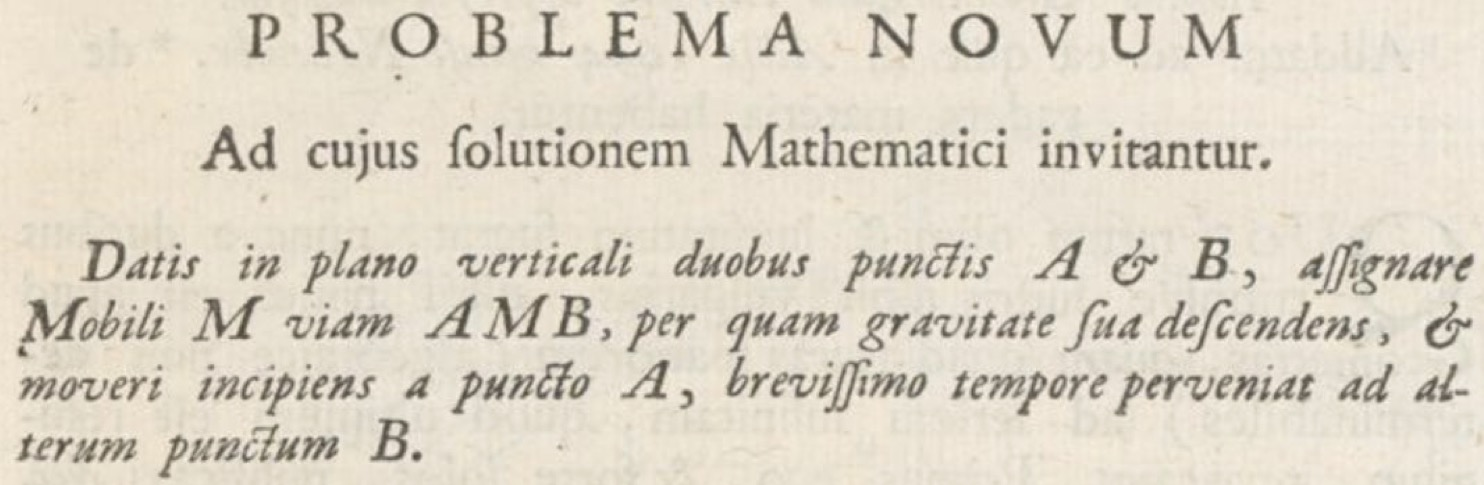
\includegraphics[width=0.8\textwidth]{chapters/020-variation/images/latein.jpg}
\end{center}
Zu deutsch:
\begin{quote}
Neue Aufgabe, zu deren Lösung die Mathematiker eingeladen werden.
Gegeben zwei Punkte $A$ und $B$ in einer vertikalen Ebene, finde
die Bahn $AMB$ eines Punktes $M$, der unter der Wirkung seines
Gewichtes in kürzester Zeit vom Punkt $A$ zum anderen Punkt $B$ absteigt.
\end{quote}
Die Situation der Aufgabenstellung ist in
Abbildung~\ref{buch:variation:fig:brachistochronenproblem}
dargestellt.
Bernoulli hat als Lösung gefunden, dass die Kurve eine Ausschnitt
aus einer Zykloide (in der Abbildung grau) sein muss.
Seine Lösung beruhte auf der Beobachtung, dass sich das Problem analog
zu einem Lichtausbreitungsproblem ist, für welches Fermat bereits
eine Lösung gefunden hat.

Da die Reibung vernachlässigt wird, ist die Energie des Massepunktes
erhalten.
Sie setzt sich aus der potenziellen und der kinetischen Energie
zusammen.
Die potenzielle Energie ist $-mgy$, die kinetische Energie ist
$\frac12mv^2$.
Die Energieerhaltung wird daher zu
\[
E=\frac12mv^2-mgy
\qquad\Rightarrow\qquad
v
=
\sqrt{2g}\!\sqrt{\frac{E}{gm}+y}
=
\!\sqrt{2(C+y)}.
\]
Durch Wahl einer anderen Zeiteinheit kann die Gleichung noch weiter
vereinfacht zu
\(
v = \sqrt{C+y}
\)
vereinfacht werden.
Gesucht ist also die zeitlich kürzeste Bahn eines Teilchens, 
dessen Geschwindigkeit auf bekannte Art $v(y)$ von der vertikalen
Koordinate abhängt.

%
% Das Fermat-Problem
%
\subsection{Das Fermat-Prinzip}
Bereits Fermat hat erkannt, dass das Brechnungsgesetz von Snellius
als Lösung eines Extremalproblems verstanden werden kann.

\begin{satz}[Fermat]
Sie $c/n_i$ die Geschwindigkeit, mit der sich Licht im Medium $M_i$
ausbreitet.
Ein Lichtstrahl von $A_1$ nach $A_2$ geht durch denjenigen Punkt $B$ 
auf der Grenzfläche zwischen den Medien, für den sich die Sinus der
Winkel $\alpha_i$ zwischen den Strahlen und der Normalen zur Grenzfläche
umgekehrt wie die $n_i$ verhalten, wenn also das Brechungsgesetz
\[
\frac{\sin\alpha_1}{\sin\alpha_2}
=
\frac{n_2}{n_1}
\]
gilt.
\end{satz}

\begin{proof}
Ohne der Beschränkung der Allgmeinheit können wir auf die Betrachtung
einer Ebene beschränken, die die beiden Punkte $A_i$ enthält und senkrecht
auf der Grenzfläche steht.
Wir dürfen weiter annehmen, dass die $x$-Achse in der Grenzfläche liegt 
und die Punkte $A_i$ die Koordinaten $(x_i,y_i)$ und der Punkt $B$ die
Koordinaten $(x,0)$ hat.
Es ist derjenige Punkt $x$ zu bestimmen, für den die Lichtzeit entlang 
des Pfades $A_1BA_2$ minimal wird.
Diese Zeit ist
\begin{align*}
t
&=
\frac{\overline{A_1B}}{c/n_1}
+
\frac{\overline{BA_2}}{c/n_2}
\\
ct
&=
n_1\overline{A_1B}
+
n_2\overline{A_2B}
\\
&=
n_1\!\sqrt{(x-x_1)^2 + y_1^2}
+
n_2\!\sqrt{(x_2-x)^2 + y_2^2}
\end{align*}
Das Minimum wird bei einer Nullstelle der Ableitung nach $x$ gefunden,
also bei einer Lösung der Gleichung
\begin{align*}
0
&=
n_1\frac{2(x_1-x)x}{\sqrt{(x_1-x)^2+y_1^2}}
+
n_2\frac{-2(x-x_2)x}{\sqrt{(x_2-x)^2+y_2^2}}.
\intertext{Indem man den zweiten Term auf der rechten Seite auf die linke
Seite bringt und durch $x$ dividiert, erhält man}
n_1
\frac{x_1-x}{\sqrt{(x_1-x)^2+y_1^2}}
&=
n_2
\frac{x-x_2}{\sqrt{(x_2-x)^2+y_2^2}}.
\end{align*}
Der Nenner ist auf beiden Seiten die Hypothenuse eines rechtwinkligen
Dreiecks, welches als Ankathete die Normale zur Grenzfläche hat.
Der Zähler ist die Gegenkathete des Winkels $\alpha_i$ zwischen der
Hypothenuse und der Normalen.
Daher ist der Quotient der Sinus des Winkels oder
\begin{equation}
n_1 \sin\alpha_1 = n_2 \sin\alpha_2.
\label{buch:variation:problem:eqn:snelliusinvariante}
\end{equation}
Die Gleichung~\eqref{buch:variation:problem:eqn:snelliusinvariante}
ist gleichbedeutend mit dem Brechungsgesetz
\[
\frac{\sin\alpha_1}{\sin\alpha_2}
=
\frac{n_2}{n_1}
\]
von Snellius.
\end{proof}

Der Satz von Fermat etabliert das Brechungsgsetz also Lösung eines
Extremalproblems.
Die Natur wählt für einen Lichtstrahl den zeitlich kürzesten Weg.
Der Beweis des Satzes von Fermat zeigt, dass entlang des Lichtstrahls
an jeder Grenzfläche zwischen Medien die Bedingung
\eqref{buch:variation:problem:eqn:snelliusinvariante}
erfüllt.
Wenn die optische Dichte $n$ eine Funktion von $n(y)$ ist, dann
wird der Lichtstrahl nicht nur in diskreten Punkten geknickt, sondern
entlang des ganzen Strahles gekrümmt.
Folgt der Strahl der Kurve $x(y)$, die mit der vertikalen den Winkel
$x'(y) = \tan\alpha(y)$ einschliesst.
Damit lässt sich auch die Sinus-Funktion ausdrücken, es gilt
\[
\sin\alpha(y)
=
\frac{x'(y)}{\pm\!\sqrt{x'(y)^2+1}}.
\]
Aus der Form~\eqref{buch:variation:problem:eqn:snelliusinvariante}
des Brechungsgesetztes wird dann die Gleichung
\begin{equation}
n_1\sin\alpha(y)
=
\frac{n_1(y)x'(y)}{\pm\!\sqrt{x'(y)^2+1}}
=
\operatorname{const}
\qquad\Rightarrow\qquad
\frac{n_1(y)^2x'(y)^2}{x'(y)^2+1}=C.
\label{buch:variation:eqn:fermatdgl}
\end{equation}
Dies ist eine Differentialgleichung für die Funktion $x(y)$.
Sie kann auch in die Form
\[
x'(y)^2
=
\frac{C}{(n_1(y)^2-C)}
\]
gebracht werden.

%
% Das Brachistochronenproblem als Lichtausbreitungsproblem
%
\subsubsection{Das Brachistochronenproblem als Lichtausbreitungsproblem}
Das Fermat-Prinzip besagt, dass ein Lichtstrahl, der sich in einem Medium
mit der Geschwindigkeit $c/n(y)$ ausbreitet, die Gleichung 
\eqref{buch:variation:eqn:fermatdgl} erfüllt.
Beim Brachistochronenproblem ist die Geschwindigkeit $v(y)=\!\sqrt{C-y}$ und 
damit $n(y) = c/\!\sqrt{C-y}$.
Eine Brachistochrone ist also eine Kurve, die die aus
\eqref{buch:variation:eqn:fermatdgl} folgende Gleichung
\begin{equation}
\frac{x'(y)^2}{(1+x'(y)^2)(C-y)} = K
\label{buch:variation:problem:eqn:bernoullidgl}
\end{equation}
erfüllen.

%
% Die Bernoullische Lösung
%
\subsubsection{Die Bernoullische Lösung}
Bernoulli hat gefunden, dass die Brachistochrone ein Zykloidenbogen ist.
Dies lässt sich dadurch verifizieren, dass man die Parametrisierung
einer Zykloide in die
Gleichung~\eqref{buch:variation:problem:eqn:bernoullidgl}
einsetzt.
Die Zykloide hat die Parametrisierung
\[
\left.
\begin{aligned}
x &= r(\varphi - \sin\varphi) 
\\
y &= r(1-\cos\varphi)
\end{aligned}
\right\}
\quad
\text{mit der Ableitung}
\quad
\left\{
\begin{aligned}
\dot{x}(\varphi) &= r(1-\cos\varphi)\\
\dot{y}(\varphi) &= r\sin\varphi
\end{aligned}
\right.
\]
für $\varphi\in\mathbb{R}$.
Die Ableitung ist
\[
x'(y)
=
\frac{\dot{x}(\varphi)}{\dot{y}(\varphi)}
=
\frac{1-\cos\varphi}{\sin\varphi}.
\]
Eingesetzt in \eqref{buch:variation:problem:eqn:bernoullidgl}
wird daraus
\[
\frac{\dot{x}(\varphi)^2}{
(\dot{y}(\varphi)^2 +\dot{x}(\varphi)^2)
(C-r(1-\cos\varphi))
}
=
\frac{(1-\cos\varphi)^2}{
((1-\cos\varphi)^2+\sin^2\varphi)
(C-r+r\cos\varphi)
}
=
K.
\]
Ausmultiplizieren im Nenner ergibt
\[
\frac{(1-\cos\varphi)^2}{
(1-2\cos\varphi+\cos^2\varphi+\sin^2\varphi)
(C-r+r\cos\varphi)
}
=
\frac{1-\cos\varphi}{
2(C-r+r\cos\varphi)
}
\]

%
% Das Brachistochronenproblem als Variationsproblem
%
\subsection{Das Brachistochronenproblem als Variationsproblem
\label{buch:variation:problem:subsection:variationsproblem}}
Die Bernoullische Lösung des Brachistochronenproblems verwendet die
Analogie zum Fermat-Prinzip.
Eine solche Analogie ist nur selten möglich, daher soll das Problem
jetzt in eine Form gebracht werden, in die auch viele ähnliche
Optimierungsproblem gebracht werden können.

Wir erinnern daran, dass die Geschwindigkeit des Massepunktes durch
$v(y)=\sqrt{C-y}$ gegeben ist.
Damit lässt sich die Zeit berechnen, die der Massepunkt entlang der
Lösungskurve braucht, wenn man diese als Funktion $y(x)$ mit beschreibt.
Die Punkte $A$ und $B$ sollen die $x$-Koordinaten $a$ bzw.~$b$ haben.
Für das Kurvenstück zwischen den $x$-Koordinaten $x$ und $x+\Delta x$
braucht der Massepunkt die Zeit
\[
\frac{ \sqrt{\Delta x^2 + \Delta y^2} }{v(y)}
=
\frac{ \sqrt{1 + y'(x)^2} }{ v(y) } \Delta x.
\]
Die Zeit ist das Integral
\begin{equation}
t
=
\int_a^b \frac{\sqrt{1+y'(x)^2}}{v(y(x))}\,dx
=
\int_a^b \sqrt{\frac{1+y'(x)^2}{C-y(x)}}\,dx.
\label{buch:variation:problem:eqn:brachint}
\end{equation}
Der Integrand auf der rechten Seite hängt nur von den Funktion $y(x)$
und $y'(x)$ ab.
Dies kommt vor allem daher, dass die Geschwindigkeit nur von $y$ abhängt,
nicht auch noch von $x$.
Im Allgemeinen wird man also davon ausgehen müssen, dass der Integrand
auch noch von $x$ abhängt.
Die Variationsrechnung befasst sich mit Problemen, in denen Funktionen
gefunden werden müssen, die ein Integral wie das in
\eqref{buch:variation:problem:eqn:brachint}
minimiert oder maximiert werden müssen.

\begin{definition}[Lagrange-Funktion des Brachistochronenproblems]
Die Lagrange-Funk\-tion des Brachistochronenproblems ist der
Integrand des Integrals
\eqref{buch:variation:problem:eqn:brachint},
\index{Lagrange-Funktion}%
also die Funktion
\[
L(x,y,y')
=
\sqrt{\frac{1+y^{\prime 2}}{C-y}}.
\]
\end{definition}

%
% Funktionale
%
\subsection{Funktionale
\label{buch:variation:problem:subsection:funktionale}}
Die Variationsrechnung löst Optimierungsproblem, die von einer
Funktion abhängen.
Um dies mathematisch präzis zu fassen, ist zunächst nötig, die Menge
der in Frage kommenden Funktionen so einzuschränken, dass die interessierende
Grösse überhaupt wohldefiniert ist.

%
% Vektorräume
%
\subsubsection{Vektorräume}
Zunächst sind die gemeinsamen algebraischen Eigenschaften zu charakterisieren,
die wir von den für unsere Untersuchungen zweckmässigen Funktionenmengen
erwarten.

\begin{definition}[Vektorraum]
Ein Vektorraum über den reellen Zahlen $\mathbb{R}$ ist einem Menge $V$ mit
zwei Operationen, der Addition und der Multiplikation mit Skalaren
\begin{align*}
    +\colon V\times V         &\to V : (u,v)\mapsto u+v
&
\cdot\colon \mathbb{R}\times V&\to V : (\lambda,v) \mapsto\lambda v
\end{align*}
mit den folgenden Eigenschaften.
\begin{enumerate}
\item
Es gelten die Assoziativgesetze
\begin{align*}
(u+v)+w&=u+(v+w)&&\text{für alle $u,v,w\in V$}\\
(\lambda \mu)v&=\lambda(\mu v)&&\text{für alle $\lambda,\mu\in\mathbb{R},\;v\in V$.}
\end{align*}
\item
Es gibt einen Vektor $0\in V$ mit der Eigenschaft $0+v=v$ für alle
Vektoren $v\in V$.
\item
Zu jedem Vektor $v\in V$ gibt es den entgegengesetzten Vektor $-v\in V$
mit der Eigenschaft, dass $-v+v=0$ ist.
\item
Die Addition von Vektoren ist kommutativ: $u+v=v+u$ für alle $u,v\in V$.
\item
Es gelten die Distributivgesetze 
\begin{align*}
(\lambda + \mu) v &= \lambda v + \mu v
	&\quad\text{für alle $\lambda,\mu\in\mathbb{R},\;v\in V$}\\
\lambda(u+v)      &= \lambda u + \lambda v
	&\quad\text{für alle $\lambda\in\mathbb{R},\;u,v\in V$}
\end{align*}
\end{enumerate}
\end{definition}

Die Mengen $\mathbb{R}^n$ erfüllen die genannten Eigenschaften, sind
also Vektorräume.
Die Definition eines Vektorraums ist aber viel allgemeiner, insbesondere
gehören dazu auch Mengen von Funktionen.
Damit wird es möglich, die Berechnungen in $\mathbb{R}^n$ auf Funktionen
auszudehnen.
Zum Beispiel bilden die stetigen Funktionen auf einem Intervall einen
Vektorraum, wie das folgende Beispiel zeigt.

\begin{beispiel}
Die Menge
\[
C([a,b])
=
\{f\colon[a,b]\to\mathbb{R}\mid \text{$f$ ist stetig}\}
\]
der stetigen Funktionen bildet einen Vektorraum.
Die Operationen sind die punktweise Addition von Funktionen und die
Multiplikation der Werte mit Skalaren, für $f,g\in C([a,b])$ und
$\lambda\in \mathbb{R}$ ist
\begin{align*}
(f+g)(x) &= f(x)+g(x)
&&\text{und}&
(\lambda f)(x) &= \lambda f(x).
\end{align*}
Entscheidend ist, dass die Addition von Funktionen und die Multiplikation
mit Skalaren nicht aus der Menge herausführt.
Tatsächlich wird in der Analysis gezeigt, dass die Summe stetiger Funktionen
wieder stetig ist und dass die Funktion $x\mapsto \lambda f(x)$ stetig,
wenn $f$ stetig ist.
Die übrigen Eigenschaften sind ebenfalls erfüllt, da sie bereits für die
Funktionswerte erfüllt sind.
\end{beispiel}

%
% Norm und Grenzwerte
%
\subsubsection{Norm und Grenzwerte}
Um Analysis zu betreiben, muss man ausdrücken können, dass eine Folge
von Funktionen konvergiert.
Dazu ist ein Abstandsbegriff zwischen Funktionen nötig.

\begin{definition}[Norm, normierter Raum]
Eine {\em Norm} auf einem Vektorraum $V$ ist eine Abbildung
\index{Norm}%
$\|\cdot\|\colon V\to\mathbb{R}^+_0$ mit nichtnegativen reellen Werten
und den folgenden Eigenschaften
\begin{itemize}
\item Definitheit: $\|v\|\ge 0$ für $v\in V$ mit Gleichheit 
genau dann, wenn $v=0$.
\index{Definitheit}%
\item Absolute Homogenität: Für alle Vektoren $v\in V$ und
\index{Homogenität}%
$\lambda\in\mathbb{R}$ gilt $\|\lambda v\| = |\lambda|\, \|v\|$.
\item Dreiecksungleichung: für alle Vektoren $u,v\in V$ gilt
\index{Dreiecksungleichung}%
$\|u+v\|\le \|u\|+\|v\|$.
\end{itemize}
Ein {\em normierter Raum} ist ein Vektorraum mit einer Norm.
\index{normierter Raum}%
\end{definition}

\begin{beispiel}
Der Vektorraum der stetigen Funktionen kann mit der Supremum-Norm
\[
\|f\| = \sup_{x\in[a,b]} |f(x)|
\]
zu einem normierten Raum gemacht werden.
Die Definitheit ist durch die Definition offensichtlich sichersgtellt.
Für $\|\lambda f\|$ finden wir
\[
\|\lambda f\|
=
\sup_{x\in[a,b]} |\lambda f(x)|
=
|\lambda|\,
\sup_{x\in[a,b]} |f(x)|
=
|\lambda|\, \|f\|,
\]
was die Homogenität zeigt.
Die Dreiecksungleichung folgt aus
\begin{align*}
\|f+g\|
&=
\sup_{x\in[a,b]} |f(x)+g(x)|
\\
&\le
\sup_{x\in[a,b]} (|f(x)|+|g(x)|)
\\
&\le
\sup_{x\in[a,b], y\in[a,b]} (|f(x)|+|g(y)|)
\\
&=
\sup_{x\in[a,b]} |f(x)|
+
\sup_{y\in[a,b]} |g(y)|
=
\|f\| + \|g\|.
\qedhere
\end{align*}
\end{beispiel}

Mit einer Norm ist es jetzt möglich, die Konvergenz von Folgen und den
Begriff des Grenzwertes zu definieren.

\begin{definition}[Cauchy-Folge, Grenzwert]
Eine Folge $(x_n)_{n\in\mathbb{N}}$ in $V$ in einem normierten Raum $V$
mit der Norm $\|\cdot\|$
heisst eine Cauchy-Folge, wenn es für jedes $\varepsilon>0$ eine
\index{Cauchy-Folge}%
$N\in \mathbb{N}$ gibt derart, dass
\[
\| x_n - x_m \| < \varepsilon
\quad\forall n,m\ge N.
\]
Der Vektor $x\in V$ heisst {\em Grenzwert} der Folge $(x_n)_{n\in\mathbb{N}}$,
\index{Grenzwert}%
wenn es zu jedem $\varepsilon > 0$ ein $N\mathbb{N}$ gibt derart, dass
\[
\|x_n-x\| < \varepsilon 
\quad\forall n\ge N.
\]
Die Folge $(x_n)_{n\in\mathbb{N}}$  in $V$ heisst {\em konvergent}, wenn
\index{konvergent}%
$x$ der Grenzwert von $(x_n)_{n\in\mathbb{N}}$ ist.
\end{definition}

Der durch die Supremum-Norm definierte Konvergenzbegriff ist die gleichmässige
Konvergenz.
Zur Erinnerung:
Eine Folge $f_n$ von Funktionen heisst gleichmässig konvergent gegen die
Funktion $f$, wenn es zu jedem
$\varepsilon >0$ ein $N\in\mathbb{N}$ gibt derart, dass
\[
|f_n(x) - f(x)|<\varepsilon\quad\forall n>N\text{ und }x\in [a,b].
\]
Die Supremum-Norm ist
\[
\|f_n(x) - f(x)\|
=
\sup_{x\in[a,b]} |f_n(x)-f(x)| < \varepsilon
\]
für alle $n>N$.
Dies ist genau die Konvergenz in der Norm $\|\cdot\|$.
Aus der Analysis ist bekannt, dass eine gleichmässig konvergente 
Funktionenfolge gegen eine stetige Funktion konvergiert.

\begin{definition}[Banach-Raum]
Ein normierter Raum $V$ heisst ein {\em Banach-Raum},
\index{Banach-Raum}%
wenn jede Cauchy-Folge in $V$ einen Grenzwert hat.
\end{definition}

\begin{beispiel}
Die Menge $C^1([0,2])$
der stetigen Funktionen auf dem Intervall $[0,2]$ ist ein normierter
Raum mit der Norm
\[
\|f\|_1
=
\int_0^2 |f(x)|\,dx,
\]
die auch die $L^1$-Norm heisst.
\index{L1-Norm@$L^1$-Norm}%
Zunächst ist nachzuprüfen, dass dies tatsächlich eine Norm ist.
Die Definitheit und die Homogenität von $\|\cdot\|_1$ ist klar, nur
die Dreiecksungleichung erfordert etwas Arbeit.
Für Funktionen $f,g\in L^1([0,2])$ gilt
\begin{align*}
\|f+g\|_1
&=
\int_0^2 |f(x)+g(x)|\,dx
\\
&\le 
\int_0^2 |f(x)|+|g(x)|\,dx
=
\int_0^2 |f(x)|\,dx
+
\int_0^2 |g(x)|\,dx
=
\|f\|_1+\|g\|_1,
\end{align*}
was die Dreeicksungleichung beweist.

Eine Cauchy-Folge in der $L^1$-Norm muss aber nicht unbedingt einen
stetigen Grenzwert haben.
Die Funktionen
\(
f_n(x) =
\begin{cases}
x^n&\quad x< 1\\
1&\quad x\ge 1
\end{cases}
\)
haben die $L^1$-Norm
\begin{align*}
\|f_n-f_m\|_1
=
\int_0^2 |f_n(x)-f_m|\,dx
\\
&=
\biggl|\int_0^1 x^n-x^m\,dx\biggr|
=
\biggl[
\biggl|
\frac{1}{n+1}x^{n+1}
-
\frac{1}{m+1}x^{m+1}
\biggr|
\biggr]_0^1
\\
&=
\biggl|
\frac{1}{n+1}
-
\frac{1}{m+1}\biggr|.
\end{align*}
Wegen
\[
\|f_n-f_m\|_1
<\varepsilon
\]
für $n,m>2/\varepsilon$ ist $f_n$ eine Cauchy-Folge in $L^1$.
In $L^1$ konvergiert die Folge $f_n$ gegen die Funktion
\[
f(x)
=
\begin{cases}
0&\quad x< 1\\
1&\quad x\ge 1.
\end{cases}
\]
Diese Funktion ist aber nicht stetig, da sie bei $x=1$ einen
Sprung hat.
Bezüglich der $L^1$-Norm ist $C^1([a,b])$ als im Allgemeinen
kein Banach-Raum.
\end{beispiel}

%
% Stetige und differenzierbare Funktionen
%
\subsubsection{Stetige und differenzierbare Funktionen}
Mit der Norm lässt sich auch die Stetigkeit von Abbildungen zwischen
normierten Räumen definieren.

\begin{definition}[Stetigkeit]
Eine Funktion $f\colon U\to V$ zwischen normierten Räumen heisst
{\em stetig im Punkt} $x\in U$, wenn es zu jedem $\varepsilon > 0$
\index{stetig in einem Punkt}%
ein $\delta > 0$
gibt derart, dass
\(
\|f(x)-f(y)\| < \delta
\)
wenn
\(
\|x-y\|<\varepsilon
\).
Eine Funktion $f\colon U\to V$ heisst {\em stetig}, wenn sie in
jedem Punkt von $U$ stetig ist.
\end{definition}

Das Bild einer Folge $x_n\in U$, die gegen $x_0\in U$ konvergiert,
ist eine Folge $f(x_n)$ in $V$.
Man sagt, $y\in V$ sei der Grenzwert von $f(x)$ für $x\to x_0$,
wenn $f(x_n)$ für jede solche Folge $x_n$ gegen $y$ konvergiert.
Der Grenzwert wird auch
\[
\lim_{x\to x_0} f(x)
=
y
\]
geschrieben.
Stetige Funktionen zeichnen sich wie in der Analysis der Funktionen
einer Variablen dadurch aus, dass der Grenzwert der Werte der Funktion
auf einer konvergenten Folge mit dem Funktionswert des Grenzwertes
übereinstimmt.

\begin{satz}
Eine Funktion $f\colon U\to V$ ist genau dann stetig im Punkt $x\in U$,
wenn für jede Folge $x_n$ in $U$ mit Grenzwert $x$ die Folge $f(x_n)$
konvergent ist und
\[
\lim_{n\to\infty} f(x_n) = f(x).
\]
Eine lineare Funktion $f\colon U\to V$ ist genau dann stetig,
wenn für jede Nullfolge $x_n$ in $U$ 
\[
\lim_{n\to \infty} f(x_n) = 0
\]
gilt.
\end{satz}

\begin{definition}
Eine Funktion $f\colon U\to V$ zwischen normierten Räumen heisst
differenzierbar im Punkt $x\in U$ wenn es eine lineare Funktion
$Df(x_0)\colon U\to V$ gibt derart, dass
\[
f(x+v) =f(x) + Df(x_0)\cdot v + o(v),
\]
wobei $o(v)$ bedeutet, dass für diese Funktion
\[
\frac{o(v)}{|v|}\to 0
\quad\text{für $v\to 0$}
\]
gilt.
\end{definition}

Funktionen auf einem Vektorraum mit reellen Werten weren auch
{\em Funktionale} genannt.
\index{Funktional}
Vor dem 20.~Jahrhundert wurde häufig ein Untersschied zwischen
Funktionen von endlich vielen reellen Variablen und Funktionen
von einem unendlichdimensionalen Vektorraum gemacht.
Die Entwicklungen dieses  Abschnittes haben gezeigt, dass eine
solche Unterscheidung nicht gerechtfertigt ist.
Es ist lediglich notwendig, die Definitionen allgemein genug zu
fassen und sich jederzeit über die Funktionenmenge und die zu
verwendende Norm Rechenschaft abzulegen.


%
% 2-fundamtenallemma.tex
%
% (c) 2023 Prof Dr Andreas Müller
%
\section{Das Fundamentallemma
\label{buch:variation:section:fundamentallemma}}
\kopfrechts{Das Fundamentallemma}
Im Fall des endlichdimensionalen Extremalproblems ist aus der
Forderung, dass alle Richtungsableitung verschwinden müssen, 
die Bedingung geworden, dass
\[
v\cdot\grad f = 0
\]
sein muss für alle Vektoren $v\in\mathbb{R}^n$.
Wir haben daraus geschlossen, dass der Gradient $\grad f=0$
sein muss.
Wir hatten dies das endlichdimensionale Fundamentallemma genannt,
wegen $e_k\cdot \grad f = D_kf$ war es eine ziemliche Selbstverständlichkeit.
Bei der Lösung von Variationsproblemen, wo es nicht um endlichdimensionale
Vektoren und das Skalarprodukt, sondern um Funktionen und Integrale
geht, brauchen wir eine ähnliche Aussage für Funktionen.

%
% Positive glatte Funktionen mit kompaktem Träger
%
\subsection{Positive glatte Funktionen mit kompaktem Träger}
Die Aussage des Fundamentallemmas für endlichdimensionale Vektoren 
folgte sofort aus der Tatsache, dass es für jedes $k$ einen Vektor
$e_k$ gibt, der nur in der Koordinaten $k$ von $0$ verschieden ist.
Natürlich gibt es auch Funktionen, die nur in genau einem Punkt
von $0$ verschieden sind.
Eine solche Funktion ist aber im allgemeinen nicht differenzier-
oder integrierbar.
In diesem Abschnitt soll daher gezeigt werden, dass es unendlich
oft stetig differnzierbare Funktionen gibt, die nur in einem beliebig
kleinen vorgegebenen Intervall $\ge 0$ sind.

\begin{definition}[Träger]
Der {\em Träger} einer Funktion $f\colon X\to\mathbb{R}$ ist die Menge
\index{Träger}%
\[
\supp f = \{ x\in X\mid f(x)\ne \}.
\]
\end{definition}

Gesucht ist also eine beliebig oft stetig differenzierbare Funktion,
deren Träger in einem vorgegebenen Intervall $[a,b]$ enthalten ist.
Wir konstruieren so eine Funktion in zwei Schritten.

\input{chapters/020-variation/fig/f.tex}

\begin{satz}
\label{buch:variation:fundamentallemma:satz:glatt}
Die Funktion
\[
f(x)
=
\begin{cases}
e^{-1/x}&\qquad x>0\\
0&\qquad x\le 0
\end{cases}
\]
(siehe auch Abbildung~\ref{buch:variation:fundamentallemma:fig:glatt})
ist beliebig oft stetig differenzierbar.
\end{satz}

\begin{proof}
Es ist klar, dass die Funktion $f$ beliebig oft stetig differenzierbar
ist in jedem Punkt $x\ne 0$.
Es ist also nur nachzuweisen, dass $f(x)$ im Punkt $0$ beliebig
oft stetig differenzierbar ist.

Die ersten drei Ableitungen von $f(x)$ sind
\begin{align}
f'(x) &= \frac{1}{x^2} f(x)
\label{buch:variation:fundamentallemma:eqn:f1}
\\
f''(x) &= \frac{1-2x}{x^4}f(x)
\notag
\\
f'''(x) &= \frac{6x^2-6x+1}{x^6}f(x).
\notag
\end{align}
Daraus lässt sich die Vermutung ableiten, dass
\begin{equation}
f^{(n)}(x)
=
\frac{p_{n-1}(x)}{x^{2n}} f(x)
\label{buch:variation:fundamentallemma:eqn:fabl}
\end{equation}
ist, wobei $p_k(x)$ ein Polynom vom Grad $k$ ist.
Wir beweisen diese Vermutung mit Hilfe von vollständiger Induktion.
Die Induktionsverankerung für die $0$-te Ableitung ist trivial.

Wir nehmen jetzt im Sinne der Induktionsannahme an, dass die $n$-te
Ableitung die Form \eqref{buch:variation:fundamentallemma:eqn:fabl}
hat.
Wir müssen zeigen, dass dann auch $f^{(n+1)}(x)$ diese Form hat.
Dazu berechnen wir
\begin{align}
f^{(n+1)}(x)
&=
\frac{d}{dx}
\frac{p_n(x)}{x^{2n}} f(x)
\notag
\\
&=
\frac{p_n'(x)}{x^{2n}} f(x)
-2n
\frac{p_n(x)}{x^{2n+1}} f(x)
+
\frac{p_n(x)}{x^{2n}} f'(x).
\notag
\intertext{Mit der ersten Ableitung
\eqref{buch:variation:fundamentallemma:eqn:f1} wird dies zu}
&=
\frac{p_n'(x)}{x^{2n}} f(x)
-2n
\frac{p_n(x)}{x^{2n+1}} f(x)
+
\frac{p_n(x)}{x^{2n}} \frac{1}{x^2}f(x)
\notag
\\
&=
\frac{x^2p_n'(x) -2nxp_n(x)+p_n(x)}{x^{2n+2}} f(x).
\label{buch:variation:fundamentallemma:eqn:induktionsschritt}
\end{align}
Die Ableitung $p_n'(x)$ ist ein Polynom vom Grad $n-1$ und damit
ist $x^2p_n'(x)$ ein Polynom vom Grad $n+1$.
Ebenso ist $xp_n(x)$ ein Polynom vom Grad $n+1$ während
$p_n(x)$ ein Polynom vom Grad $n$ ist.
Der Zähler von
\eqref{buch:variation:fundamentallemma:eqn:induktionsschritt}
ist
\[
p_{n+1}(x)
=
x^2p_n'(x)+(1 -2nx)p_n(x),
\]
ein Polynom vom Grad $n+1$.
Damit ist der Induktionsschritt erfolgreich und die Behauptung betreffend
die Form von $f^{(n)}(x)$ ist bewiesen.

Es ist jetzt nur noch zu zeigen, dass der Grenzwert von $f^{(n)}(x)$
für $x\to 0+$ verschwindet.
Da das Polynom $p_n(x)$ stetig ist, folgt
\[
\lim_{x\to 0}
f^{(n)}(x)
=
\lim_{x\to 0}\frac{p_n(x)}{x^{2n}}f(x)
=
p_n(0) \lim_{t\to\infty} t^{2n} e^{-t}
=
0.
\]
Damit ist die beliebige stetige Differenzierbarkeit an der Stelle
$x=0$ gezeigt.
\end{proof}

Die Funktion $f(x)$ von 
Satz~\ref{buch:variation:fundamentallemma:satz:glatt} 
erfüllt noch nicht die Forderung, dass sie nur in einem vorgegebenen
Intervall von $0$ verschieden ist.

\input{chapters/020-variation/fig/g.tex}

\begin{satz}
\label{buch:variation:fundamentallemma:satz:gab}
Sei $f(x)$ die Funktion von
Satz~\ref{buch:variation:fundamentallemma:satz:glatt}.
Dann ist
\[
g_{a,b}(x)
=
f(x-a) f(b-x)
\]
eine unendlich oft stetig differenzierbare, nichtnegative Funktion mit Träger
$\supp g_{a,b}=(a,b)$.
\end{satz}

Die Funktionen $g_{a,b}(x)$ sind beliebig oft differenzierbar und nur im
Intervall $[a,b]$ von $0$ verschieden und sogar positiv.
Weil sie stetig sind, sind sie auch integrierbar, man kann also das
Integral über $\mathbb{R}$ berechnen und die Funktion damit normieren.
Die neue Funktion
\[
\frac{1}{N}
\tilde{g}_{a,b}(x)
\qquad\text{mit}\;
N
=
\int_{-\infty}^{\infty}g_{a,b}(x)\,dx
=
\int_a^b g_{a,b}(x)\,dx
\]
ist immer noch beliebig oft stetig differenzierbar und hat zusätzlich die
Eigenschaft
\[
\int_{-\infty}^{\infty}
\tilde{g}_{a,b}(x)\,dx
=
\int_a^b
\tilde{g}_{a,b}(x)\,dx
=
1.
\]
Wir formulieren dieses Resultat als Satz.

\begin{satz}
\label{buch:variation:satz:gabeins}
Zu jedem Intervall $[a,b]$ gibt es eine beliebig oft stetig
differenzierbare Funktion $g(x)$, genau das Intervall $[a,b]$
als Träger hat und deren Integral über $[a,b]$ den Wert $1$ hat.
\end{satz}

%
% Das Fundamentallemma
%
\subsection{Das Fundamentallemma}
Mit der Funktion $g_{a,b}(x)$ von
Satz~\ref{buch:variation:fundamentallemma:satz:gab}
lässt sich jetzt das Fundamentallemma in der folgenden Form
leicht beweisen.

\begin{satz}[Fundamentallemma]
\label{buch:variation:fundamentallemma:satz:fundamentallemma}
Wenn für die stetige Funktion $f\colon[a,b]\to\mathbb{R}$ 
\begin{equation}
\int_a^b f(x)\varphi(x)\,dx = 0
\label{buch:variation:fundamentallemma:eqn:fundamentalbed}
\end{equation}
gilt für jede beliebig oft stetig differenzierbare Funktion $\varphi(x)$ 
dann ist $f(x)=0$.
Das Resultat gilt selbst dann, wenn
\eqref{buch:variation:fundamentallemma:eqn:fundamentalbed}
nur für beliebig oft stetig differenzierbare Funktionen $\varphi(x)$ 
gilt, die ausserdem an den Intervallenden verschwinden:
$\varphi(a)=\varphi(b)=0$.
\end{satz}

\begin{proof}
Wir zeigen mit Hilfe eines Widerspruchs, dass es keinen Punkt $x_0\in[a,b]$
geben kann, für den $f(x_0)\ne 0$ ist.
Dazu nehmen wir also an, dass $f(x_0)\ne 0$ ist.
Falls $f(x_0)<0$ ist, ersetzen wir $f$ durch $-f$, 
die Bedingung
\eqref{buch:variation:fundamentallemma:eqn:fundamentalbed}
ändert sich dadurch nicht.
\input{chapters/020-variation/fig/fundamentallemma.tex}
Wir dürfen daher annehmen, dass $f(x_0)>0$ ist
(Abbildung~\ref{buch:variation:fundamentallemma:fig:beweis}).
Da $f$ stetig ist, gibt es ein Intervall $[x_0-\varepsilon,x_0+\varepsilon]$
derart, dass $f(x)> \frac12 f(x_0)$ für
$x\in[x_0-\varepsilon,x_0+\varepsilon]$ gilt.
Dann gilt für das Integral
\[
\int_a^b
f(x)
g_{x_0-\varepsilon,x_0+\varepsilon} (x)
\,dx
>
\frac{f(x_0)}{2}
\int_a^b
g_{x_0-\varepsilon,x_0+\varepsilon} (x)
\,dx
>
0
\]
im Widerspruch zur Bedingung
\eqref{buch:variation:fundamentallemma:eqn:fundamentalbed}.
Der Widerspruch zeigt, dass $f(x)=0$ sein muss.
\end{proof}

%
% Skalarproduktformulierung des Fundamentallemmas
%
\subsection{Skalaproduktformulierung des Fundamentallemmas}
Die Richtungsableitung einer Funktion endlich vieler Variablen 
konnte als Skalarprodukt mit dem Gradienten geschrieben werden und
das Fundamentallemma hat besagt, dass der Gradient verschwindet,
wenn alle Richtungsableitungen verschwinden.
Diese Schlussweise ist auch für Funktionen möglich, wenn man Funktionen
ein Skalarprodukt definieren kann.

\begin{definition}[$L^2$-Skalarprodukt]
Das {\em Skalarprodukt} zweier quadratintegrierbarer Funktion $f$ und $g$
auf dem Intervall $[a,b]$ ist definiert durch
\[
\langle f,g\rangle
=
\int_a^b f(x)g(x)\,dx.
\]
\end{definition}

\begin{satz}[Fundamentallemma, Skalarproduktform]
Wenn für eine stetige Funktion $f\colon[a,b]\to\mathbb{R}$ das Skalarprodukt
\[
\langle f,\varphi\rangle = 0
\]
ist für jede unendlich oft differenzierbare Funktion $\varphi$ auf dem
Intervall $[a,b]$, dann ist $f=0$.
\end{satz}



%
% 3-eulerlagrange.tex
%
% (c) 2023 Prof Dr Andreas Müller
%
\section{Die Euler-Lagrange Differentialgleichung
\label{buch:variation:section:eulerlagrange}}
\kopfrechts{Die Euler-Lagrange Differentialgleichung}
Das Neuartige an der Aufgabenstellung des Brachistochronenproblems
war, dass eine Funktion gesucht war, so dass ein damit gebildetes
Integral eine Minimaleigenschaft erfüllt.
Für die damalige Mathematik war die Aufgabe, eine Funktion zu finden,
nicht neu.
Die Theorie der Differentialgleichungen war bereits entwickelt,
Newton hat die Infinitesimalrechnung ja erfunden, um damit die
Bewegungsgleichungen der Physik zu formulieren und zu lösen.
In einer Differentialgleichung werden Werte und Ableitungen einer
Funktion an einer einzigen Stelle miteinander verbunden.
Etwas salop formuliert sagt die Differentialgleichung in jedem
Punkt, in welche Richtung und mit welcher Krümmung die Funktionskurve
weiter zu zeichnen ist.

Im Brachistochronenproblem tragen aber alle Werte der gesuchten
Funktion zum Integral bei, es scheint daher auf den ersten Blick
nicht möglich, das Problem durch schrittweise Konstruktion
``von Punkt zu Punkt'' der Lösungskurve zu konstruieren.

Bernoullis Lösung des Brachistochrononproblems beruht auf der
Beobachtung, dass sich die Bedinung für die schnellste Bahn
durch eine Bedingung ersetzen lässt, die in jedem einzelnen
Punkt ausgewertet werden kann.
Das von ihm verwendete Fermat-Prinzip wurde ursprünglich ebenfalls
als eine globale Eigenschaft eines Lichtstrahls formuliert.
Aus dem Fermat-Prinzip folgt aber das Brechungsgesetz, welches
sagt, dass die Richtung eines Strahls in einem Punkt genau dann
ändert, wenn sich dort auch der Brechungsindex der beiden Medien
ändert.
Das Fermat-Prinzip ist also ein Beispiel dafür, wie eine globale
Bedingung erfüllt werden kann, indem einer lokalen Regel in jedem
Punkt gefolgt wird.

Es ist das Verdienst von Euler und Lagrange, zu erkennen, dass diese
Übersetzung eines globalen Variationsproblems in ein lokales 
Problem immer möglich ist.
Es entsteht dabei die Euler-Lagrange-Differentialgleichung, welche
die Problemstellung auf die Lösung einer Differentialgleichung
reduziert.
Damit ist ein allgemein anwendbares Lösungsverfahren gefunden.
Zu einem Variationsproblem lässt sich immer eine Differentialgleichung
finden, welche die gesuchte Funktion als Lösung hat.

In diesem Abschnitt soll dieser indirekte Weg der Lösung von
Variationsaufgaben dargestellt werden.
Wir werden später zeigen, dass diese Vorgehensweise nicht immer
erfolgreich sein kann.
Zum Beispiel werden wir in Kapitel~\ref{buch:chapter:nichtdiff}
Variationsprobleme kennenlernen, deren Lösungskurven nicht
differenzierbar sind und daher auch nicht von einer Differentialgleichung
gefunden werden können.
Im Kapitel~\ref{buch:chapter:direkt} werden daher die sogenannten
direkten Methodn vorgestellt, die den Umweg über eine
Differentialgleichung vermeiden.

%
% Die Lagrange-Funktion
%
\subsection{Die Lagrange-Funktion
\label{buch:variation:eulerlagrange:subsection:lagrange-funktion}}
Wir betrachten Variationsproblem der folgenden Art.
Gesucht ist eine auf dem Intervall $[x_0,x_1]$ definirte
Funktion $y(x)$, die das Integral
\begin{equation}
I(y)
=
\int_{x_0}^{x_1}
F(x, y(x), y'(x))
\,dx
\label{buch:variation:eulerlagrange:eqn:funktional}
\end{equation}
maximiert oder minimiert.
Der Ausdruck~\eqref{buch:variation:eulerlagrange:eqn:funktional}
wird ein Funktional genannt.
Die Funktion
\[
F
\colon
\mathbb{R}\times
\mathbb{R}\times
\mathbb{R}
\to
\mathbb{R}
\]
von drei Variablen heisst die {\em Lagrange-Funktion}
des Funktionals \eqref{buch:variation:eulerlagrange:eqn:funktional}.

\begin{beispiel}
Die Lagrange-Funktion des Brachistochronenproblems ist
\[
F(x,y,y')
=
\sqrt{ \frac{1+y^{\prime 2}}{y} }.
\]
Die Funktion hängt nicht von $x$ ab, was bedeutet, dass eine
Verschiebung in $x$-Richtung die Form der Lösungsfunktion des
Variationsproblems nicht ändert.
\end{beispiel}

\begin{beispiel}
\label{buch:variation:eulerlagrange:beispiel:gerade}
Wir formulieren die Aufgabe, die kürzeste Verbindung der Punkte
$(x_0,y_0)$ und $(x_1,y_1)$ in einer Ebene zu finden, als Variationsproblem.
Die Länge einer Kurve $y(x)$ ist das Integral
\[
l(y)
=
\int_{x_0}^{x_1}
\sqrt{1+y'(x)^2}\,dx.
\]
Daraus lesen wir ab, dass die Lagrange-Funktion dieses Variationsproblems
\begin{equation}
F(x,y,y') = \sqrt{1+y^{\prime 2}}
\label{buch:variation:eulerlagrange:eqn:geradeL}
\end{equation}
ist.
Die Funktion hängt weder von $x$ noch von $y$ ab.
Dies ist auch zu erwarten, denn die Länge einer Kurve hängt nicht davon
ob, wo in der Ebene sie platziert ist.
Eine Verschiebung in $x$-Richtung würde das $x$-Argument ändern,
eine Verschiebung in $y$-Richtung die $y$-Werte.
Wäre $F$ von $x$ oder $y$ abhängig, könnte auch die Länge der Kurve
davon abhängen.
\end{beispiel}

%
% Euler-Lagrange_Differentialgleichung
%
\subsection{Euler-Lagrange-Differentialgleichung
\label{buch:variation:eulerlagrange:subsection:dgl}}
\input{chapters/020-variation/fig/variation0.tex}
Das Maximum oder Minimum einer Funktionen mehrere Variablen wurde
gefunden, indem die Richtungsableitung berechnet und $=0$ gesetzt
wurde.
Um die Funktion zu bestimmen, die ein Funktional $I(y)$ zu einem
Maximum oder Minimum macht, versuchen wir, die Idee der Richtungsableitung
für ein Funktional nachzuahmen.
Wir nehmen daher an, dass $y(x)$ eine Funktion ist, die das Funktional
$I(y)$ zu einem Minimum macht.
Für die Richtungsableitung addieren wir ein Vielfaches einer
Funktion $\eta(x)$, die Summe $y(x)+\varepsilon\eta(x)$ entspricht
dann einer Geraden mit Richtung $\eta(x)$ im Funktionenraum
(Abbildung~\ref{buch:variation:fig:variation0}).
Die Funktionen $y(x)+\varepsilon\eta(x)$ sind aber nur dann Kandidaten
für eine Lösung des Problems, wenn immer noch
\begin{align*}
y(x_0) + \varepsilon \eta(x_0) &= y_0
&&\text{und}&
y(x_1) + \varepsilon \eta(x_1) &= y_1
\end{align*}
gilt.
Dies ist nur möglich, wenn $\eta(x_0)=\eta(x_1)=0$ ist.

Wir berechnen jetzt die Ableitung der Funktion
$\varepsilon\mapsto I(y+\varepsilon\eta )$ an der Stelle $\varepsilon=0$.
Da die Intervallgrenzen nicht von $\varepsilon$ abhängen, können wir
die Ableitung unter das Integral nehmen:
\begin{align*}
\frac{d}{d\varepsilon}
I(y+\varepsilon\eta)
&=
\int_{x_0}^{x_1}
\frac{d}{d\varepsilon}
F(x,y(x)+\varepsilon\eta(x),y(x)+\varepsilon\eta'(x))
\,dx.
\intertext{Da $F$ differenzierbar ist, kann die Ableitung mit der
Kettenregel berechnet werden, sie ist}
&=
\int_{x_0}^{x_1}
\frac{\partial F}{\partial y}
(x,y(x)+\varepsilon\eta(x),y(x)+\varepsilon\eta'(x))
\eta(x)
\\
&\qquad
+
\frac{\partial F}{\partial y'}
(x,y(x)+\varepsilon\eta(x),y(x)+\varepsilon\eta'(x))
\eta'(x)
\,dx.
\intertext{Uns interessiert aber nur der Wert an der Stelle $\varepsilon=0$,
er ist}
\frac{d}{d\varepsilon}
I(y+\varepsilon\eta)
\bigg|_{\varepsilon=0}
&=
\int_{x_0}^{x_1}
\frac{\partial F}{\partial y}
(x,y(x),y'(x))
\,
\eta(x)
+
\frac{\partial F}{\partial y'}
(x,y(x),y'(x))
\,
\eta'(x)
\,dx
=0.
\end{align*}
Das Integral hängt von den verschiedenen Faktoren $\eta(x)$ und
von $\eta'(x)$ in den beiden Termen unter dem Integral ab.
Wir integrieren den zweiten Term partiell 
\begin{align*}
\int_{x_0}^{x_1}
\frac{\partial F}{\partial y'}(x,y(x),y'(x))\,\eta'(x)\,dx
&=
\biggl[
\frac{\partial F}{\partial y'}(x,y(x),y'(x))\,\eta(x)
\biggr]_{x_0}^{x_1}
\\
&\qquad
-
\int_{x_0}^{x_1}
\frac{d}{dx}
\frac{\partial F}{\partial y'}(x,y(x),y'(x))\,\eta(x)\,dx.
\end{align*}
Da $\eta(x_0)=\eta(x_1)=0$ verschwindet der erste Term
auf der rechten Seite, es bleibt
\[
\frac{d}{d\varepsilon}
I(y+\varepsilon\eta)
\bigg|_{\varepsilon=0}
=
\int_{x_0}^{x_1}
\biggl(
\frac{\partial F}{\partial y}
(x,y(x),y'(x))
-
\frac{d}{dx}
\frac{\partial F}{\partial y'}
(x,y(x),y'(x))
\biggr)
\eta(x)
\,dx.
\]
Dies kann auch als Skalarprodukt
\[
\biggl\langle 
\frac{\partial F}{\partial y}
(x,y(x),y'(x))
-
\frac{d}{dx}
\frac{\partial F}{\partial y'}
(x,y(x),y'(x))
,
\eta(x)
\biggr\rangle
=
0
\]
geschrieben werden.
Da dies für jede differenzierbare Funktion $\eta$ mit Randwerten
$\eta(x_0)=\eta(x_1)$ gelten muss, folgt nach dem
Fundamentallemma~\ref{buch:variation:fundamentallemma:satz:fundamentallemma},
der folgende Satz. 

\begin{satz}[Euler-Lagrange]
\label{buch:variation:eulerlagrange:satz:eulerlagrange}
Wenn die mindestens zweimal stetig differenzierbare Funktion $y(x)$
unter allen solchen Funktionen mit $y(x_0)=y_0$ und $y(x_1)=y_1$
das Funktional
\[
I(y)
=
\int_{x_0}^{x_1}
F(x,y(x),y'(x))\,dx
\]
zu einem Maximum oder Minimum macht, dann ist $y(x)$ eine Lösung der
gewöhnlichen Differentialgleichung
\begin{equation}
\frac{d}{dx}
\frac{\partial F}{\partial y'}(x,y(x),y'(x))
-
\frac{\partial F}{\partial y}(x,y(x),y'(x))
=
0.
\label{buch:variation:eulerlagrange:eqn:eulerlagrange}
\end{equation}
Sie heisst die {\em Euler-Lagrange-Differentialgleichung}.
\end{satz}

Eine Lösung des Variationsproblems kann also als Lösung der
Euler-Lagrange-Dif\-fe\-ren\-tial\-glei\-chung mit den Randwerten
$y(x_0)=x_0$ und $y(x_1)=y_1$ gefunden werden.
Die Bedingung ist notwendig, aber nicht hinreichend.
Wie bei der Bestimmung eines Extremums bei Funktionen endlich
vieler Variablen garantiert das Verschwinden der Richtungsableitung
nicht, dass auch tatsächlich ein Extremum vorliegt.
Man sagt daher auch, dass eine Lösung $y(x)$ der
Euler-Lagrange-Differentialgleichung das Funktional $I(y)$
stationär macht.

Eine weitere Einschränkung ist, dass die Herleitung der
Euler-Lagrange-Differential\-gleichung vorausgesetzt hat,
dass die Lösungsfunktion $y(x)$ mindestens zweimal 
stetig differenzierbar ist.
Es gibt aber durchaus Variationsprobleme, deren Lösungen
nicht differenzierbar sind, dazu mehr im Kapitel~\ref{buch:chapter:nichtdiff}.

\begin{beispiel}
\label{buch:variation:eulerlagrange:beispiel:gerade}
Wir lösen das Variationsproblem von Beispiel
\ref{buch:variation:eulerlagrange:beispiel:gerade}
mit der Lagrange-Funk\-tion
\eqref{buch:variation:eulerlagrange:eqn:geradeL}.
Da die Lagrange-Funktion nicht von $y$ abhängt, bleibt von der 
Euler-Lagrange-Gleichung nur
\[
\frac{d}{dx}
\frac{\partial L}{\partial y'}(x,y(x),y'(x))
=
0
\]
übrig.
Berechnung der Ableitung liefert
\begin{equation}
\frac{\partial}{\partial y'}
\sqrt{1+y^{\prime 2}}
=
\frac{y'}{\sqrt{1+y^{\prime 2}}}.
\label{buch:variation:eulerlagrange:eqn:ableitungFyp}
\end{equation}
Die Ableitung nach $x$ ergibt
\begin{align*}
\frac{d}{dx}
\frac{\partial}{\partial y'}
\sqrt{1+y^{\prime 2}}
&=
\frac{d}{dx}
\frac{y'}{\sqrt{1+y^{\prime 2}}}
\\
&=
\frac{
y''\sqrt{1+y^{\prime 2}}-y'\cdot \frac{y'y''}{\sqrt{1+y^{\prime 2}}}
}{
1+y^{\prime 2}
}
\\
&=
y''
\frac{
1+y^{\prime 2}-y^{\prime 2}
}{
(1+y^{\prime 2})^{\frac32}
}.
\intertext{Die Euler-Lagrange-Differentialgleichung ist daher}
0
&=
\frac{y''}{(1+y^{\prime 2})^{\frac32}} .
\end{align*}
Der Nenner auf der rechten Seite ist immer $\ge 1$, die Gleichung kann
also nur erfüllt sein, wenn $y''=0$ ist.
Die Funktion $y(x)$ muss also eine lineare Funktion $y=ax+b$ sein.
Die Randbedingung wird erfüllt für die Geradengleichung
\[
y(x)
=
\frac{y_1-y_0}{x_1-x_0}(x-x_0) + y_0.
\]
Kürzeste Verbindungen in der Ebene sind daher Geraden.
\end{beispiel}

%
% Freie Randbedingungen
%
\subsection{Freie Randbedingungen
\label{buch:variation:eulerlagrange:subsection:freierb}}
In der Herleitung der Euler-Lagrange-Differentialgleichung wurde angenommen,
dass die Endpunkte der Lösungsfunktion durch $y(x_0)=y_0$ und $y(x_1)=y_1$
fest vorgegeben sind.
Diese Voraussetzung soll in diesem Abschnitt abgeschwächt werden.
Die Funktionswerte in den Endpunkten sollen also nicht mehr fest
vorgegeben sein.

\begin{beispiel}
\label{buch:variation:eulerlagrange:beispiel:freiegerade}
Im Beispiel~\ref{buch:variation:eulerlagrange:beispiel:gerade}
wurde die kürzeste Kurve zwischen zwei Punkten in der Ebene
gesucht und wie erwartet eine Gerade als Lösung gefunden.
Wenn die Werte $y_0$ und $y_1$ jetzt nicht mehr vorgegeben sind,
wird die kürzeste Verbindung zwischen den beiden Geraden
$x=x_0$ und $x=x_1$ gesucht.
Die Lösung dieses Problems ist nicht eindeutig, jede horizontale
Strecke mit $y_0=y_1$ ist eine Lösung.
\end{beispiel}

Das Beispiel zeigt, dass es im Allgemeinen immer noch die Vorgabe
eines der beiden Randwerte braucht, um die Lösung eindeutig zu
bestimmen.
Wir lösen daher die folgende Aufgabe.

\begin{aufgabe}
Gesucht ist eine zweimal stetig differnzierbare Funktion $y(x)$ auf
dem Intervall $[x_0,x_1]$ mit $y(x_0)=y_0$, die das Integral
\[
I(y)
=
\int_{x_0}^{x_1} F(x,y(x),y'(x))\,dx
\]
zu einem Extremum macht.
Am rechten Ende des Intervalls ist der Funktion $y(x)$ keine
Randbedingung auferlegt.
\end{aufgabe}

\begin{proof}[Lösung]
\input{chapters/020-variation/fig/variation1.tex}
Sei $y(x)$ eine Lösung der Aufgabe und sei $y_1:=y(x_1)$ der Wert
der Lösung am rechten Rand des Intervalls.
Wir berechnen wieder die Variation von $I(y)$ mit Hilfe von
stetig differenzierbaren Funktionen $\eta(x)$, die jetzt aber 
nur noch die Bedingungn $\eta(x_0)=0$ erfüllen müssen
(Abbildung~\ref{buch:variation:fig:variation1}).
Die Richtungsableitung ist wie früher
\begin{align*}
\frac{d}{d\varepsilon}
I(y+\varepsilon\eta)
\bigg|_{\varepsilon=0}
&=
\frac{d}{d\varepsilon}
\int_{x_0}^{x_1}
F(x,y(x)+\varepsilon\eta(x),y'(x)+\varepsilon\eta'(x))\,dx
\\
&=
\int_{x_0}^{x_1}
\frac{\partial F}{\partial y}(x,y(x),y'(x)) 
\eta(x)
+
\frac{\partial F}{\partial y'}
(x,y(x),y'(x))
\eta'(x)
\,dx
\intertext{und mit partieller Integration}
&=
\biggl[
\frac{\partial F}{\partial y'}(x,y(x),y'(x)) \eta(x)
\biggr]_{x_0}^{x_1}
\\
&\qquad
+
\int_{x_0}^{x_1}
\biggl(
\frac{\partial F}{\partial y}(x,y(x),y'(x))
-
\frac{d}{dx}
\frac{\partial F}{\partial y'}(x,y(x),y'(x))
\biggr)
\,
\eta(x)
\,dx.
\end{align*}
Im Gegensatz zu früher können wir jetzt aber nicht mehr
schliessen, dass der erste Term verschwindet, da $y(x_1)$ nicht
mehr als $=0$ verausgesetzt wird.
Vielmehr erhalten wir für die erste Variation
\begin{equation*}
\delta I(y)
=
\frac{\partial F}{\partial y'} (x_1,y(x_1),y'(x_1)) \eta(x_1)+
\int_{x_0}^{x_1}
\biggl(
\frac{\partial F}{\partial y}(x,y(x),y'(x))
-
\frac{d}{dx}
\frac{\partial F}{\partial y'}(x,y(x),y'(x))
\biggr)
\,
\eta(x)
\,dx.
\end{equation*}
Die Klammer im Integral ist von der Euler-Lagrange-Differentialgleichung
her bekannt, aber es ist ein weiterer hinzugekommen, der genau dann
verschwindet wenn auch $\eta(x_1)=0$ ist.

Dann ist $y(x)$ natürlich erst recht eine Lösung des Problems, das
Funktional $I(y)$ mit den {\em zwei} Randbedingungen
$y(x_0)=y_0$ und $y(x_1)=y_1$ zu einem Extremum zu machen, also
muss die Funktion $y(x)$ sicher die Euler-Lagrange-Differentialgleichung
erfüllen.
Die Klammer im Integral wird daher verschwinden, die Variation
reduziert sich auf den ersten Term
\[
\delta I(y)
=
\frac{\partial F}{\partial y'} (x_1,y(x_1),y'(x_1)) \eta(x_1)
=
0.
\]
Sie verschwindet nur dann für alle zulässigen Funktionen $\eta(x)$, wenn
\begin{equation*}
\frac{\partial F}{\partial y'}(x_1,y(x_1),y'(x_1))=0
\end{equation*}
gilt.
Dies ist eine zusätzliche Randbedingung für die Funktion $y(x)$, geschrieben
in einer impliziten Form.
\end{proof}

Wir halten das Resultat der Aufgabenlösung als Satz fest:

\begin{satz}
\label{buch:variation:eulerlagrange:satz:zusaetzlicherb}
Wenn die zweimal stetig differenzierbare Funktion $y(x)$ mit dem
Randwert $y(x_0)=y_0$ das Integral
\[
I(y)
=
\int_{x_0}^{x_1} F(x,y(x),y'(x))\,dx
\]
zu einem Extremum macht, dann erfüllt sie am rechten Intervallende
die Randbedingung
\begin{equation}
\frac{\partial F}{\partial y'}(x_1,y(x_1),y'(x_1))=0.
\label{buch:variation:eulerlagrange:eqn:zusaetzlicherb}
\end{equation}
zusätzlich zur Euler-Lagrange-Gleichung für die Lagrange-Funktion $F$.
\end{satz}

\begin{beispiel}
\label{buch:variation:eulerlagrange:beispiel:einseitigegerade}
Wir betrachten wieder das Funktional
\[
I(y)
=
\int_{x_0}^{x_1}
\sqrt{1+y^{\prime 2}(x)}
\,dx
\]
mit der einzigen Randbedingung $y(x_0)=y_0$, der Funktionswert auf 
der rechten Seite ist nicht vorgebeben.
Der Satz~\eqref{buch:variation:eulerlagrange:satz:zusaetzlicherb}
besagt zunächst, dass die Lösungsfunktion wieder eine Gerade sein
muss, da die Euler-Lagrange-Gleichung erfüllt sein muss.
Zusätzlich muss aber auch die Randbedingung
\eqref{buch:variation:eulerlagrange:eqn:zusaetzlicherb}
am rechten Ende des Intervalls erfüllt sein.
Die Ableitung der Lagrange-Funktion ist in diesem Fall durch
\eqref{buch:variation:eulerlagrange:eqn:ableitungFyp}
gegeben, es muss also
\[
\frac{y'(x_1)}{\sqrt{1+y'(x_1)^2}}
=
0
\qquad\Rightarrow\qquad y'(x_1)=0
\]
gelten.
Die Lösung ist daher wie erwartet eine horizontale Strecke.
\end{beispiel}



%
% 5-hoehereableitungen.tex
%
% (c) 2023 Prof Dr Andreas Müller
%
\section{Höhere Ableitungen
\label{buch:variation:section:hoehereableitungen}}
\kopfrechts{Höhere Ableitungen}
Das Beispiel der Spline-Interpolation in
Abschnitt~\ref{buch:nichtdiff:section:splines}
zeigt, dass es manchmal
nötig ist, höhere Ableitungen als die erste in einem Funktional
zu berücksichtigen.
In diesem Abschnitt wird die Theorie der ersten Variation auf
Funktionale erweitert, die von beliebigen Ableitungen der Funktion $y(x)$
abhängen.

%
% Lagrange-Funktion mit höheren Ableitungen
%
\subsection{Lagrange-Funktion mit höheren Ableitungen}
Die Euler-Lagrange-Differentialgleichung wurde bisher für Funktionale
hergeleitet, deren Lagrange-Funktion von $x$, der Funktion $y(x)$ und
der ersten Ableitung $y'(x)$ abhängen.

\begin{definition}
Eine Funktion $L(x,y,y',\dots,y^{(n)})$ heisst eine Lagrange-Funktion
der Ordnung $n$.
\index{Lagrange-Funktion $n$-ter Ordnung}%
\end{definition}

\begin{beispiel}
Das Variationsproblem für die Spline-Integration hat die Lagrange-Funktion
zweiter Ordnung
\[
L(x,y,y',y'') = y^{\prime\prime 2}
\]
verwendet.
\end{beispiel}

Ein elastischer Stab speichert bei Verbiegung Energie, deren Dichte
entlang des Stabes proportional zur Krümmung ist.
Ist $s\mapsto \gamma(s)\in\mathbb{R}^2$ eine differenzierbare
Parametrisierung einer ebenen Kurve, die die Form eines dünnen elastischen
Stabes beschreibt, dann ist die Gesamtenergie des Stabes bis auf
eine Konstante durch das Integral
\[
E
=
\int_a^b \kappa(s)^2 \,ds
\]
gegeben
Ist $s$ ein Bogenlängenparameter, also $|\dot{\gamma}(s)|=1$, dann ist
die Krümmung die zweite Ableitung, also
\[
I = \int_a^b \ddot{\gamma}(s)^2\,ds.
\]
Diese Parameterdarstellung ist aber nicht die Form, in der wir bis jetzt
Kurven in der Ebene beschreiben konnten.

Sei $y(x)$ eine Funktion, deren Graph einen elastisch verbogenen Stab
in der Ebene beschreibt.
Die Krümmung des Graphen kann nach
\[
\kappa(x)
=
\frac{y''(x)}{(1+y'(x)^2)^{\frac32}}
\]
berechnet werden.
Die Energie des Stabes wird dann
\[
E
=
\int_a^b \frac{y''(x)^2}{(1+y'(x)^2)^3}\,dx.
\]
Die Lagrange-Funktion des Problems der Biegung eines Stabes ist daher
\[
L(x,y,y',y'')
=
\frac{y^{\prime\prime 2}}{(1+y^{\prime 2})^3}.
\]

%
% Die verallgemeinerte Euler-Lagrange-Differentialgleichung
%
\subsection{Die verallgemeinerte Euler-Lagrange-Differentialgleichung}
Auch für ein Variationsproblem mit einer Lagrange-Funktion, die höhere
Ableitungen enthält, lässt sich mit der mehr oder weniger gleichen
Vorgehensweise eine Differentialgleichung für die gesuchte Funktion
$y(x)$ herleiten.
Wie auch im Beispiel zur Spline-Interpolation in
Abschnitt~\ref{buch:nichtdiff:section:splines} angedeutet, wird es
notwendig sein, mehrmals partiell zu integrieren.

Sei also $L(x,y,y',\dots,y^{(n)})$ eine Lagrange-Funktion $n$-ter Ordnung
und sei eine Funktion $y(x)$ gesucht, die ein kritischer Punkt des Funktionals
\[
I(y)
=
\int_a^b L\bigl(x,y(x),y'(x),\dots,y^{(n)}(x)\bigr)\,dx
\]
ist.
Wir berechnen wieder die erste Variation mit Hilfe einer beliebig
oft differenzierbaren Funktion $\eta(x)$, welche in den Endpunkten
des Intervalls zusammen mit allen Ableitungen verschwindet.
Die Variation ist definiert als die Richtungsableitung in Richtung
von $\eta(x)$ als
\begin{align*}
\delta I
&=
\frac{d}{dt}
\int_a^b
L\bigl(x,y(x)+t\eta(x),y'(x)+t\eta'(x),\dots,y^{(n)}(x)+t\eta^{(n)}(x)\bigr)
\,dx\biggl|_{t=0}.
\intertext{Durch Ableitung nach $t$ finden wir}
&=
\int_a^b
\frac{\partial L}{\partial y}\bigl(x,y(x),y'(x),\dots,y^{(n)}(x)\bigr)
\,
\eta(x)
+
\frac{\partial L}{\partial y'}\bigl(x,y(x),y'(x),\dots,y^{(n)}(x)\bigr)
\,
\eta'(x)
\\
&\qquad
+
\dots
+
\frac{\partial L}{\partial y^{(n)}}\bigl(x,y(x),y'(x),\dots,y^{(n)}(x)\bigr)
\,
\eta^{(n)}(x)
\,dx.
\end{align*}
Die Terme mit Ableitungen von $\eta(x)$ können durch partielle
Integration in Terme umgewandelt werden, die nur die Funktion 
$\eta(x)$ enthalten:
\begin{align*}
\delta I
&=
\int_a^b
\frac{\partial L}{\partial y^{(k)}}
\bigl(x,y(x),y'(x),\dots,y^{(n)}(x)\bigr)
\,
\eta^{(k)}(x)
\,dx
\\
&=
\biggl[
\frac{\partial L}{\partial y^{(k)}}
\bigl(x,y(x),y'(x),\dots,y^{(n)}(x)\bigr)
\,
\eta^{(k-1)}(x)
\biggr]_a^b
\\
&\qquad
-
\int_a^b
\frac{d}{dx}
\frac{\partial L}{\partial y^{(k)}}
\bigl(x,y(x),y'(x),\dots,y^{(n)}(x)\bigr)
\,
\eta^{(k-1)}(x)
\,dx.
\intertext{Da die Ableitungen von $\eta(x)$ in den Intervallenden
verschwinden, ist dies gleichbedeutend mit}
&=
-\int_a^b \frac{d}{dx} \frac{\partial L}{\partial y^{(k)}}
\bigl(x,y(x),y'(x),\dots,y^{(n)}(x)\bigr)
\,
\eta^{(k-1)}(x)
\,dx.
\intertext{Durch Iterieren dieser Rechnung erhalten wir}
&=
(-1)^{k}
\int_a^b
\frac{d^k}{dx^k}
\frac{\partial L}{\partial y^{(k)}}
\bigl(x,y(x),y'(x),\dots,y^{(n)}(x)\bigr)
\,
\eta(x)
\,dx.
\end{align*}
Die Variation kann jetzt als
\begin{align*}
\delta I
&=
\int_a^b
\biggl(
\frac{\partial L}{\partial y}
-
\frac{d}{dx}
\frac{\partial L}{\partial y'}
+
\frac{d^2}{dx^2}
\frac{\partial L}{\partial y''}
-
\dots
+
(-1)^n
\frac{d^n}{dx^n}
\frac{\partial L}{\partial y^{(n)}}
\biggr)
\,
\eta(x)
\,dx
\end{align*}
geschrieben werden.
Die Variation $\delta I$ muss für jede Wahl von $\eta(x)$ verschwinden,
daher folgt aus dem Fundamentallemma, dass $y(x)$ die Differentialgleichung
\begin{equation}
\frac{\partial L}{\partial y}
-
\frac{d}{dx}
\frac{\partial L}{\partial y'}
+
\frac{d^2}{dx^2}
\frac{\partial L}{\partial y''}
-
\dots
+
(-1)^n
\frac{d^n}{dx^n}
\frac{\partial L}{\partial y^{(n)}}
=
0
\label{buch:variation:hohere:eqn:eulerlagrange}
\end{equation}
erfüllen muss.
Man beachte, dass wir in dieser Rechnung stillschweigend annehmen,
dass die Funktion $y(x)$ genügend oft stetig differenzierbar ist,
so dass die einzelnen Terme der Differentialgleichung
\eqref{buch:variation:hohere:eqn:eulerlagrange} wohldefiniert sind.

\begin{satz}[Euler-Lagrange-Differentialgleichung]
Eine genügend oft differenzierbare Funktion $y(x)$ ist ein stationärer
Punkt des Integrals
\[
I
=
\int_a^b
L\bigl(x,y(x),y'(x),\dots,y^{(n)}(x)\bigr)
\,dx
\]
mit der Lagrange-Funktion $n$-ter Ordnung $L(x,y,y',\dots,y^{(n)})$,
wenn sie die die Euler-Lagrange-Differentialgleichung
\eqref{buch:variation:hohere:eqn:eulerlagrange} erfüllt.
\end{satz}



%
% 6-mehrerefunktionen.tex
%
% (c) 2023 Prof Dr Andreas Müller
%
\section{Varationsproblem für mehrere Funktionen
\label{buch:variation:section:mehrerefunktionen}}
\kopfrechts{Mehrere Funktionen}
Nur sehr spezielle Kurven können dargestellt werden als Graphen
einer Funktion $y(x)$.
Als Lösung des isoperimetrischen Problems wird ein Kreis erwartet,
der sich sicher nicht so darstellen lässt.
Die natürliche Darstellung eines Kreises ist eine Parameterdarstellung
$t\mapsto(\cos t,\sin t)$, auf die die bisherige Theorie nicht
vorbereitet ist.

%
% Lagrange-Funktion für mehrere Funktionen
%
\subsection{Lagrange-Funktion für mehrere Funktionen
\label{buch:variation:mehrerefunction:subsection:lagrangefunktion}}
Eine Parameterdarstellung einer Kurve ist ein Vektor von Funktionen
$y_1(x),\dots,y_n(x)$.
Wir schreiben auch
\[
y(x)
=
\begin{pmatrix}
y_1(x)\\
\vdots\\
y_n(x)
\end{pmatrix}
\qquad\text{und}\qquad
y'(x)
=
\frac{d}{dx}
\begin{pmatrix}
y_1(x)\\
\vdots\\
y_n(x)
\end{pmatrix}
=
\begin{pmatrix}
y_1'(x)\\
\vdots\\
y_n'(x)
\end{pmatrix}
\]
für die Vektorfunktion und ihre erste Ableitung.

Eine {\em Lagrange-Funktion} für ein Variationsproblem wird von
der unabhängigen Variablen $x$, den Funktionswerten aller Funktionen
$y_1(x),\dots,y_n(x)$ und den Ableitungen $y'_1(x),\dots,y'_n(x)$
abhängen.
Sie ist also eine Funktion von $2n+1$ Variablen, die wir als
\begin{equation*}
F
\colon
\mathbb{R}^{2n+1}\to\mathbb{R}
:
(x,y_1,\dots,y_n,y'_1,\dots,y'_n)\mapsto F(x,y_1,\dots,y_n,y'_1,\dots,y'_n)
\end{equation*}
Mit dieser Schreibweise wird das Funktional, das extremal gemacht 
werden soll.
\[
I(y)
=
\int_{x_0}^{x_1}
F(x,y_1(x),\dots,y_n(x),y'_1(x),\dots,y'_n(x))\,dx.
\]
Der Fall $n=1$ ist der bereits früher behandelte.

Besonders elegant lässt sich die Theorie formulieren, wenn wir
die Lagrange-Funktion als Funktion der vektorwertigen Argumente
$y$ und $y'$ schreiben:
\begin{equation}
F
\colon
\mathbb{R}\times\mathbb{R}^n\times\mathbb{R}^n
\to
\mathbb{R}
:
(x,y,y')
\mapsto F(x,y,y').
\label{buch:variation:mehrerefunktionen:eqn:Fvektor}
\end{equation}
Das zu varierende Integral wird dann
\[
I(y)
=
\int_{x_0}^{x_1}
F(x,y(x),y'(x))
\,dx
\]
In dieser Schreibweise unterscheidet sich das Problem formal
nicht mehr vom bereits behandelten.
Es kann in dieser Form aber nicht mit der bereits hergeleiteten
Euler-Lagrange-Differentialgleichung gelöst werden, da die
Ableitung $\partial F/\partial y$ nach einem Vektor $y$ nicht
definiert ist.

%
% Ableitungen nach den Vektorargumenten
%
\subsection{Ableitungen nach den Vektorargumenten
\label{buch:variation:mehrerefunktionen:subsection:vektorableitung}}
Sei $F$ eine Lagrange-Funktion der Form
\eqref{buch:variation:mehrerefunktionen:eqn:Fvektor}.
Wir möchten die Ableitung nach den Vektorargument $y$ und $y'$ 
definieren, damit wir später im
Abschnitt~\ref{buch:variation:mehrerefunktionen:subsection:eulerlagrange}
die Euler-Lagrange-Gleichungen so kompakt wie möglich schreiben können.

Da der Vektor $y$ aus den Variablen $y_1,\dots,y_n$ besteht und $y'$
aus den $y'_1,\dots,y'_n$, ist jede der Ableitungen
\[
\frac{\partial F}{\partial y_k}
\qquad\text{und}\qquad
\frac{\partial F}{\partial y'_k}
\]
wohldefiniert.
Sie bilden zwei Vektoren, die wir als
\begin{equation}
\frac{\partial}{\partial y}
F(x,y,y')
=
\begin{pmatrix}
\frac{\partial}{\partial y_1}F(x,y,y')\\
\vdots\\
\frac{\partial}{\partial y_n}F(x,y,y')
\end{pmatrix}
\qquad\text{und}\qquad
\frac{\partial}{\partial y'} F(x,y,y')
=
\begin{pmatrix}
\frac{\partial}{\partial y'_1}F(x,y,y')\\
\vdots\\
\frac{\partial}{\partial y'_n}F(x,y,y')
\end{pmatrix}
\end{equation}
schreiben wollen.
Ist $\eta(x)$ eine vektorwertige Funktion mit Komponenten
$\eta_k(x)$, dann kann man jetzt 
die in der Variation von
$f(\varepsilon) = F(x,y(x)+\varepsilon\eta(x),y(x)+\varepsilon\eta(x))$
benötigte Ableitung nach $\varepsilon$ schreiben:
\begin{align*}
\frac{d}{d\varepsilon}f(\varepsilon)
&=
\sum_{k=1}^n
\frac{\partial}{\partial y_k}
F(x,y(x)+\varepsilon\eta(x),y'(x)+\varepsilon\eta'(x))
\eta_k(x)
\\
&\qquad
+
\frac{\partial}{\partial y'_k}
F(x,y(x)+\varepsilon\eta(x),y'(x)+\varepsilon\eta'(x))
\eta_k'(x)
\\
&=
\frac{\partial}{\partial y}
F(x,y(x),y'(x))\cdot \eta(x)
+
\frac{\partial}{\partial y'}
F(x,y(x),y'(x))\cdot \eta'(x)
\end{align*}
Der einzige Unterschied in der Notation gegenüber dem skalaren Fall
ist, dass jeweils das Skalarprodukt zur Multiplikation mit $\eta(x)$
bzw.~$\eta'(x)$ verwendet werden muss.

%
% Die Euler-Lagrange-Differentialgleichung
%
\subsection{Die Euler-Lagrange-Differentialgleichung
\label{buch:variation:mehrerefunktionen:subsection:eulerlagrange}}
Für eine Lagrange-Funktion für $r$ Funktionen $y_1(x),\dots,y_r(x)$
lässt sich die Variation des Integrals
\[
I
=
\int_a^b L(x,y_1(x),y_1'(x),\dots,y_r(x),y_r'(x))\,dx
\]
ganz analog zur einer Lagrange-Funktion
mit nur einer Funktion berechnen.
Dazu verwenden wir Funktionen $\eta_1(x),\dots,\eta_r(x)$, die
in den Endpunkten verschwinden und berechnen die Variation
\begin{align}
\delta I
&=
\frac{d}{dt}
\int_a^b
L(x,y_1(x)+t\eta_1(x),y_1'(x)+t\eta_1'(x),\dots,
y_r(x)+t\eta_r(x),y_r'(x)+t\eta_r'(x))
\,dx
\bigg|_{t=0}
\notag
\\
&=
\int_a^b
\frac{\partial L}{\partial y_1}\eta_1(x)
+
\frac{\partial L}{\partial y'_1}\eta'_1(x)
+
\dots
\frac{\partial L}{\partial y_r}\eta_r(x)
+
\frac{\partial L}{\partial y'_r}\eta'_r(x)
\,dx
\notag
\intertext{Die Terme mit Ableitungen von $\eta'_i(x)$ können durch partielle
Integration umgeformt werden:}
&=
\int_a^b
\frac{\partial L}{\partial y_1}\eta_1(x)
+\dots+
\frac{\partial L}{\partial y_r}\eta_r(x)
\,dx
+
\biggl[
\frac{\partial L}{\partial y'_1}\eta_1(x)
+
\frac{\partial L}{\partial y'_r}\eta_r(x)
\biggr]_a^b
\\
&\qquad
-
\int_a^b
\frac{d}{dx}
\frac{\partial L}{\partial y'_1}
\eta_1(x)
+
\dots
+
\frac{d}{dx}
\frac{\partial L}{\partial y'_r}
\eta_r(x).
\notag
\intertext{Der mittlere Term verschwindet, weil die Funktionen
$\eta_i(x)$ an den Intervallenden verschwinden.
Die Variation ist daher}
\delta I
&=
\int_a^b
\biggl(
\frac{\partial L}{\partial y_1}-\frac{d}{dx}\frac{\partial L}{\partial y'_1}
\biggr)\eta_1(x)
\,dx
+
\dots
+
\int_a^b
\biggl(
\frac{\partial L}{\partial y_r}-\frac{d}{dx}\frac{\partial L}{\partial y'_r}
\biggr)\eta_r(x)
\,dx.
\label{buch:variation:mehrere:eqn:summe}
\end{align}
Da die Funktionen $\eta_i(x)$ alle bis auf eine $=0$ gewählt werden können,
muss jedes der Integrale in \eqref{buch:variation:mehrere:eqn:summe}
verschwinden muss.
Nach dem Fundamentallemma folgt daher der folgende Satz.

\begin{satz}
\label{buch:variation:mehrere:satz:rfunktionen}
Das Integral
\[
\int_a^b L(x,y_1(x),y_1'(x),\dots,y_r(x),y'_r(x))\,dx
\]
mit einer Lagrange-Funktion für $r$ Funktionen $y_1(x),\dots,y_r(x)$
nimmt einen stationären Wert an für Funktionen %$y_1(x),\dots,y_r(x)$,
welche das Differentialgiechungssystem
\begin{equation}
\frac{\partial L}{\partial y_k}(x,y_1(x),y'_1(x),\dots,y_r(x),y'_r(x))
-
\frac{d}{dx}
\frac{\partial L}{\partial y'_k}(x,y_1(x),y'_1(x),\dots,y_r(x),y'_r(x))
=
0,
\label{buch:variation:mehrerefunktionen:eqn:reulerlagrange}
\end{equation}
$k=1,\dots,r$ erfüllen.
\end{satz}

In einen Variationsproblem sind im Allgemeinen geeignete Randbedingungen
notwendig, die die Lösung des Differentialgleichungssystems
\eqref{buch:variation:mehrerefunktionen:eqn:reulerlagrange}
eindeutig festlegen.

%
% Vektorform der Euler-Lagrange-Differentialgleichung
%
\subsubsection{Vektorform der Euler-Lagrange-Differentialgleichung}
Die Lagrange-Funktion $L(x,y_1,y'_1,\dots,y_r,y'_r)$ kann auch als
eine Funktion
\[
L\colon
\mathbb{R}\times\mathbb{R}^r \times \mathbb{R}^r
\to
\mathbb{R}
\]
geschrieben werden.
Die Ableitung $D_2L$ ist die Ableitung nach den Variablen $y_1,\dots,y_r$
während $D_3L$ die Ableitung nach den Variablen $y'_1,\dots,y'_r$ ist.
Gesucht ist wie früher ein stationärer Punkt des Integrals
\[
I
=
\int_a^b L(x,y(x),y'(x))\,dx,
\]
wobei $y\colon[a,b]\to\mathbb{R}^r$ eine vektorwertige Funktion ist.
Um die Variation zu bilden, brauchen wir eine vektorwertige Funktion
$\eta\colon[a,b]\to\mathbb{R}$, deren Komponenten in den Endpunkten
des Intervalls verschwinden.
Die Variation ist dann
\begin{align*}
\delta I
&=
\frac{d}{dx}
\int_a^b L(x, y(x)+t\eta(x), y'(x)+t\eta'(x))\,dx
\bigg|_{t=0}
\\
&=
\int_a^b
D_2L(x,y(x),y'(x)) \eta(x)
+
D_3L(x,y(x),y'(x)) \eta'(x)
\,dx
\intertext{$D_2L$ ist eine Linearform, die auf den Vektor $\eta(x)$ 
angewendet wird, und analog für $D_3L$.
Für den Term mit $\eta'(x)$ verwenden wir wieder partielle Integration}
&=
\int_a^b D_2L(x,y(x),y'(x))\eta(x)\,dx
+
\biggl[L(x,y(x),y'(x))\biggr]_a^b
\\
&\qquad
-
\int_a^b \frac{d}{dx}D_eL(x,y(x),y'(x)) \eta(x)\,dx.
\intertext{Da die Komponenten von $\eta(x)$ an den Intervallenden
verschwinden, fällt der mittlere Term weg und es bleibt}
&=
\int_a^b \bigl(D_2L(x,y(x),y'(x))-\frac{d}{dx}D_3L(x,y(x),y'(x))\bigr)
\eta(x)\,dx.
\end{align*}
Nach dem Fundamentallemma folgt die $r$-dimensionale
Vektor-Differentialgleichung
\[
D_2L(x,y(x),y'(x)) - \frac{d}{dx}D_3L(x,y(x),y'(x)) = 0.
\]
Beide Terme sind Linearformen auf $\mathbb{R}^r$, ihre Koeffizienten
sind die einzelnen Differentialgleichungen von
Satz~\ref{buch:variation:mehrere:satz:rfunktionen}.

%
% Parameterdarstellung von Kurven
%
\subsection{Parameterdarstellung von Kurven
\label{buch:variation:mehrerefunktionen:subsection:kurven}}
Ein Kurve im $r$-dimensionalen Raum $\mathbb{R}^r$ ist eine differenzierbare
Abbildung
\[
\gamma
\colon
\mathbb{R} \to \mathbb{R}^r
:
t \mapsto \gamma(t).
\]
Die Koordinaten von $\gamma(t)$ bilden $r$ Funktionen $\gamma_i(t)$
für $i=1,\dots,r$.
Die Ableitung nach dem Kurvenparameter $t$ ist der Tangentialvektor
\[
\frac{d}{dt}\gamma(t) = \dot{\gamma}(t),
\]
er wird mit dem Punkt bezeichnet.

Ein Variationsproblem für eine Kurve basiert auf einer Lagrange-Funktion
\[
L
\colon
\mathbb{R}\times\mathbb{R}^r\times\mathbb{R}^r
:
(t,x,\dot{x})
\mapsto
L(t,x,\dot{x}),
\]
aus der das Funktional
\begin{equation}
I(\gamma)
=
\int_{t_0}^{t_1}
L(t,\gamma(t),\dot{\gamma}(t))
\,dt
\label{buch:variation:mehrerefunktionen:eqn:funktionalkurve}
\end{equation}
abgeleitet werden kann.
Dies ist natürlich ein Variationsproblem für die $r$ Komponentenfunktionen
des Vektors $\gamma(t)$.

Die Euler-Lagrange-Differentialgleichung für das Funktional
\eqref{buch:variation:mehrerefunktionen:eqn:funktionalkurve}
ist die $r$-dimensionale Vektordifferentialgleichung
\begin{equation}
\frac{\partial L}{\partial x}(t,\gamma(t), \dot{\gamma}(t))
-
\frac{d}{dt}
\frac{\partial L}{\partial \dot{x}}(t,\gamma(t),\dot{\gamma}(t))
=
0.
\label{buch:variation:mehrerefunktionen:eqn:eulerlagrangekurve}
\end{equation}
Zusätzlich sind Randbedingungen notwendig, um die Lösung 
eindeutig festzulegen.
Lösungen der Differentialgleichung
\eqref{buch:variation:mehrerefunktionen:eqn:eulerlagrangekurve}
sind stationäre Punkte des Funktionals
\eqref{buch:variation:mehrerefunktionen:eqn:funktionalkurve}.

%
% Das homogene Problem
%
\subsection{Das homogene Variationsproblem
\label{buch:variation:mehrerefunktionen:subsection:homogen}}







%
% 6-allgemein.tex
%
% (c) 2024 Prof Dr Andreas Müller
%
\section{Die allgemeine Theorie der ersten Variation
\label{buch:variation:section:allgemein}}
\kopfrechts{Die allgemeine Theorie der ersten Variation}
In Abschnitt~\ref{buch:variation:eulerlagrange:subsection:freierb}
wurde gezeigt, wie sich in einem Variationsproblem mit vorgegebenem
Randwert nur an einem Ende des Intervalls aus der ersten Variation
automatisch eine zusätzliche Randbedingung am anderen Ende des
Intervalls ergibt.
Die Endpunkte $x_0$ und $x_1$ des Intervalls waren aber immer noch 
fest.
In diesem Abschnitt soll gezeigt werden, wie sich diese Einschränkung
aufheben lässt.

%
% Allgemeine Variation einer Funktion
%
\subsection{Allgemeine Variation einer Funktion $y(x)$
\label{buch:variation:allgemein:subsection:vary}}
In Abschnitt~\ref{buch:variation:section:eulerlagrange} wurde die
erste Variation mit Hilfe von Funktionen der Form
\begin{equation}
x
\mapsto
y(x)+\varepsilon\eta(x)
\label{buch:variation:allgemein:eqn:ansatz}
\end{equation}
konstruiert.
Mit diesem Ansatz ist es nicht möglich, die Endpunkte $x_0$ und $x_1$
des Intervalls zu varieren.
Es war zwar möglich, die $y$-Werte zu varieren, was auf die zusätzliche
Randbedingung von
Satz~\ref{buch:variation:eulerlagrange:satz:zusaetzlicherb}
geführt hat.
Wir möchten aber sogar die Intervallgrenzen varieren können, dieser
Fall wird von den bisherigen Entwicklungen nicht abgedeckt.

%
% Verallgemeinerung des Variationsansatzes
%
\subsubsection{Verallgemeinerung des Variationsansatzes}
\input{chapters/020-variation/fig/variation.tex}%
Statt des Ansatzes~\eqref{buch:variation:allgemein:eqn:ansatz}
verwenden wir jetzt eine Parametrisierung
\begin{equation}
y
\colon
[x_0(\varepsilon),x_1(\varepsilon)]
\to
\mathbb{R}
:
x\mapsto y(x,\varepsilon)
\label{buch:variation:allgemein:eqn:ansatz2}
\end{equation}
für $\varepsilon$-Werte in einer Umgebung von $0$
(Abbildung~\ref{buch:variation:fig:variation}).
Damit
\eqref{buch:variation:allgemein:eqn:ansatz2}
eine Variation der einer Funktion $y(x)$ beschreibt, soll
$y(x) = y(x,0)$ sein.
Die Funktionen $x_0(\varepsilon)$ und $x_1(\varepsilon)$ beschreiben
die Endpunkte des Definitionsintervalls der partiellen Funktion
$x\mapsto y(x,\varepsilon)$.

Der ursprüngliche Ansatz~\eqref{buch:variation:allgemein:eqn:ansatz}
ist in \eqref{buch:variation:allgemein:eqn:ansatz2} enthalten, wenn
man $x_0(\varepsilon)=x_0$, $x_1(\varepsilon)=x_1$ und
\[
y(x,\varepsilon) = y(x) + \varepsilon \eta(x)
\]
setzt.
In der Herleitung der Euler-Lagrange-Differentialgleichung wurde
entscheidend verwendet, dass man diese Funktion nach $\varepsilon$
ableiten kann.
Dass dies möglich ist, ist nach den bisherigen Forderungen an
$y(x,\varepsilon)$ nicht garantiert.
Es muss also zusätzlich Differenzierbarkeit nach $\varepsilon$
gefordert werden.

\begin{definition}[Allgemeine Variation einer Funktion]
\label{buch:variation:allgemein:def:variation}
Eine stetig nach beiden Variablen differenzierbare Funktion $y(x,\varepsilon)$
ist eine {\em allgemeine Variation} der Funktion $y(x)$, wenn es stetig
differenzierbare Funktionen
$x_0(\varepsilon)$ und $x_1(\varepsilon)$ gibt derart, dass
die partielle Funktion $x\mapsto y(x,\varepsilon)$ auf dem
Intervall $[x_0(\varepsilon),x_1(\varepsilon)]$ stetig differenzierbar
ist und für $\varepsilon=0$ mit $y(x)$ übereinstimmt: $y(x)=y(x,0)$.
Der Einfachheit halber wird die partielle Ableitung von $y(x,\varepsilon)$
nach $x$ auch
\[
y'(x,\varepsilon) = \frac{\partial y}{\partial x}(x,\varepsilon)
\]
geschrieben.
Für die Werte an den Endpunkten schreiben wir abkürzend
\begin{align*}
x_i &= x_i(0),
&
y_i &= y(x_i(0),0) = y(x_i)
&&\text{und}&
y_i'
=
y'(x_i(0),0)
=
\frac{\partial y'(x(\varepsilon),\varepsilon)}{\partial\varepsilon}
\bigg|_{\varepsilon=0}
\end{align*}
für $i=0,1$.
\end{definition}

%
% Kurven, auf denen sich die Endpunkte bewegen
%
\subsubsection{Kurven, auf denen sich die Endpunkte bewegen}
Der Ansatz~\eqref{buch:variation:allgemein:eqn:ansatz2} beschreibt
Kurven, die die beiden Punkte
\begin{align*}
P_0(\varepsilon)
&=
(x_0(\varepsilon),y(x_0(\varepsilon),\varepsilon))
&&\text{und}&
P_1
&=
(x_1(\varepsilon),y(x_1(\varepsilon),\varepsilon))
\end{align*}
miteinander verbinden.
Die Endpunkte der Kurve bewegen sich also auf den Kurven
\begin{align*}
\varepsilon
&\mapsto
P_0(\varepsilon)
=
(x_0(\varepsilon),y(x_0(\varepsilon),\varepsilon)
&&\text{und}&
\varepsilon
&\mapsto
P_1(\varepsilon)
=
(x_1(\varepsilon),y(x_1(\varepsilon),\varepsilon).
\end{align*}
Da alle beteiligten Funktionen als differenzierbar vorausgesetzt wurden,
lassen sich auch die Tangenten dieser Kurven bestimmen.
Der Richtungsvektor der Tangente im Punkt $x_i=x_i(0)$ ist
\begin{align}
\vec{r}_i(\varepsilon)
=
\frac{d}{d\varepsilon}
\begin{pmatrix}
x_i(\varepsilon)\\
y(x_i(\varepsilon),\varepsilon)
\end{pmatrix}
\bigg|_{\varepsilon=0}
\label{buch:variation:allgemein:eqn:tangential}
\end{align}
für $i=0,1$.
Die Kurve $\varepsilon\mapsto P_i(\varepsilon)$ lässt sich daher für
genügend kleine $\varepsilon$ beliebig genau durch
\[
x\mapsto
\begin{pmatrix}
x_0(0)\\
y(x,0) 
\end{pmatrix}
+
\varepsilon
\frac{d}{d\varepsilon}
\begin{pmatrix}
x_i(\varepsilon)\\
y(x_i(\varepsilon),\varepsilon)
\end{pmatrix}
\bigg|_{\varepsilon=0}
\]
approximieren.

%
% Erste Variation
%
\subsection{Erste Variation einer einzelnen Funktion
\label{buch:variation:allgemein:subsection:var1}}
Wir betrachten jetzt wieder das Funktional
\[
I(y)
=
\int_{x_0}^{x_1} F(x,y(x),y'(x)) \,dx
\]
für die Lagrange-Funktion $f(x,y,y')$.
Eine allgemeine Variation der Funktion $y(x)$ im Sinne der
Definition~\ref{buch:variation:allgemein:def:variation} macht aus
$I(y)$ eine Funktion 
\[
I(y,\varepsilon)
=
\int_{x_0(\varepsilon)}^{x_1(\varepsilon)}
F(x,y(x,\varepsilon),y'(x,\varepsilon))
\,dx
\]
von $\varepsilon$.
Davon ist wieder die Ableitung nach $\varepsilon$ an der Stelle
$\varepsilon=0$ zu ermitteln.
Sie ist
\begin{align*}
\frac{\partial}{\partial\varepsilon}I(y,\varepsilon)
&=
F(x_1(\varepsilon),y(x_1(\varepsilon),\varepsilon),
y'(x_1(\varepsilon),\varepsilon))
\frac{dx_1(\varepsilon)}{d\varepsilon}
-
F(x_0(\varepsilon),y(x_0(\varepsilon),\varepsilon),
y'(x_0(\varepsilon),\varepsilon))
\frac{dx_0(\varepsilon)}{d\varepsilon}
\\
&\qquad
+
\int_{x_0(\varepsilon)}^{x_1(\varepsilon)}
\frac{\partial F}{\partial y}(x, y(x,\varepsilon), y'(x,\varepsilon))
\frac{\partial y}{\partial \varepsilon}(x,\varepsilon)
\,dx
\\
&\qquad
+
\int_{x_0(\varepsilon)}^{x_1(\varepsilon)}
\frac{\partial F}{\partial y'}(x, y(x,\varepsilon), y'(x,\varepsilon))
\frac{\partial^2 y}{\partial x\,\partial\varepsilon}(x,\varepsilon)
\,dx
\end{align*}
An der Stelle $\varepsilon=0$ vereinfacht sich die Variation zu
\begin{align}
\delta I(y)
&=
F(x_1,y(x_1),y'(x_1))
\frac{dx_0(0)}{d\varepsilon}
-
F(x_0,y(x_0),y'(x_0))
\frac{dx_1(0)}{d\varepsilon}
\notag
\\
&\qquad
+
\int_{x_0}^{x_1}
\frac{\partial F}{\partial y}(x,y(x),y'(x))
\frac{\partial y}{\partial \varepsilon}(x,0)
\,dx
\notag
\\
&\qquad
+
\int_{x_0}^{x_1}
\frac{\partial F}{\partial y'}(x,y(x),y'(x))
\frac{\partial^2 y}{\partial x\,\partial\varepsilon}(x,0)
\,dx.
\label{buch:variation:allgemein:eqn:var1}
\end{align}
Die Ableitung $y'$ im zweiten Integral kann mit partieller Integration 
vereinfacht werden:
\begin{align*}
\int_{x_0}^{x_1}
\frac{\partial F}{\partial y'}(x,y(x),y'(x))
\frac{\partial y'}{\partial \varepsilon}(x,0)
\,dx
&=
\biggl[
\frac{\partial F}{\partial y'}(x,y(x),y'(x))
\frac{\partial y}{\partial\varepsilon}(x,0)
\biggr]_{x_0}^{x_1}
\\
&\qquad
-
\int_{x_0}^{x_1}
\frac{d}{dx}
\frac{\partial F}{\partial y'}(x,y(x),y'(x))
\frac{\partial y}{\partial\varepsilon}(x,0)
\,dx.
\end{align*}
Eingesetzt in 
\eqref{buch:variation:allgemein:eqn:var1}
ist die allgemeine Variation des Funktionals $I(y)$ daher
\begin{equation}
\begin{aligned}
\delta I(y)
&=
F(x_1,y(x_1),y'(x_1))
\frac{dx_0(0)}{d\varepsilon}
-
F(x_0,y(x_0),y'(x_0))
\frac{dx_1(0)}{d\varepsilon}
\\
&\qquad
+
\biggl[
\frac{\partial F}{\partial y'}(x,y(x),y'(x))
\frac{\partial y}{\partial\varepsilon}(x,0)
\biggr]_{x_0}^{x_1}
\\
&\qquad
+
\int_{x_0}^{x_1}
\biggl(
\frac{\partial F}{\partial y}(x,y(x),y'(x))
-
\frac{d}{dx}\frac{\partial F}{\partial y'}(x,y(x),y'(x))
\biggr)
\frac{\partial y}{\partial \varepsilon}(x,0)
\,dx.
\end{aligned}
\label{buch:variation:allgemein:eqn:variation}
\end{equation}

Sei jetzt $y(x)$ eine Funktion, die das Funktional $I(y)$ stationär macht,
für jede Wahl einer Variation von $y(x)$ ist also $\delta I(y)=0$.
Dies gilt insbesondere auch für alle Variationen, die Endpunkte der
Kurve unverändert lassen.
Für eine solche Variation verschwinden die ersten drei Terme, es bleibt
nur das Integral.
Wie früher folgt daher, dass der Ausdruck in der Klammer im Integral
verschwinden muss.
Eine Lösung des Variationsproblems muss also die
Euler-Lagrange-Differentialgleichung erfüllen.

Die verbleibenden Terme in \eqref{buch:variation:allgemein:eqn:variation}
drücken aus, wie sich das Funktional $I(y)$ ändert, wenn sich die
Endpunkte der Kurve verschieben.
Die ersten zwei Terme behandeln offensichtlich den Fall, dass die 
Intervalgrenzen verschoben werden.
Der dritte Term behandelt die Änderung, die ausschliesslich von der
Änderung des zweiten Parameters von $y(x,\varepsilon)$ ausgeht.
Der $y$-Wert kann sich auch dadurch ändern, dass $x$ variert wird.
\begin{align*}
\frac{dy(x_i(\varepsilon),\varepsilon)}{d\varepsilon}
&=
\frac{\partial y(x_i(\varepsilon),\varepsilon)}{\partial x}
\frac{dx_i(\varepsilon)}{d\varepsilon}
+
\frac{\partial y(x_i(\varepsilon), \varepsilon)}{\partial \varepsilon}
\intertext{oder an der Stelle $\varepsilon=0$}
\frac{dy(x_i(0),0)}{d\varepsilon}
&=
\frac{\partial y(x_i(0),0)}{\partial x}
\frac{dx_i(0)}{d\varepsilon}
+
\frac{\partial y(x_i(0), 0)}{\partial \varepsilon}
\intertext{Aufgelöst nach dem letzten Term ist dies}
\frac{\partial y(x_i(0), 0)}{\partial \varepsilon}
&=
\frac{dy(x_i(0),0)}{d\varepsilon}
-
\frac{\partial y(x_i(0),0)}{\partial x}
\frac{dx_i(0)}{d\varepsilon}
\end{align*}
Dies können wir in die Variation
\eqref{buch:variation:allgemein:eqn:variation}
einsetzen und erhalten
\begin{equation}
\begin{aligned}
\delta I(y)
&=
\biggl(
F(x_1,y(x_1),y'(x_1))
-
\frac{\partial y(x_1(0),0)}{\partial x}
\frac{\partial F}{\partial y'}(x_1,y(x_1),y'(x_1))
\biggr)
\frac{dx_1(0)}{d\varepsilon}
\\
&\qquad
+
\frac{\partial F}{\partial y'}(x_1,y(x_1),y'(x_1))
\frac{dy(x_1(0),0)}{d\varepsilon}
\\
&\qquad
-
\biggl(
F(x_0,y(x_0),y'(x_0))
-
\frac{\partial y(x_0(0),0)}{\partial x}
\frac{\partial F}{\partial y'}(x_0,y(x_0),y'(x_0))
\biggr)
\frac{dx_0(0)}{d\varepsilon}
\\
&\qquad
-
\frac{\partial F}{\partial y'}(x_0,y(x_0),y'(x_0))
\frac{dy(x_0(0),0)}{d\varepsilon}
\\
&\qquad
+
\int_{x_0}^{x_1}
\biggl(
\frac{\partial F}{\partial y}(x,y(x),y'(x))
-
\frac{d}{dx}\frac{\partial F}{\partial y'}(x,y(x),y'(x))
\biggr)
\frac{\partial y}{\partial \varepsilon}(x,0)
\,dx.
\end{aligned}
\label{buch:variation:allgemein:eqn:variation}
\end{equation}
Von den ersten vier Terme lassen sich jeweils zwei als ein Skalarprodukt
des Vektors
\[
\vec{f}_i
=
\begin{pmatrix}
\displaystyle
F(x_i,y(x_i),y'(x_i))
-
\frac{\partial F}{\partial y'}(x_i,y(x_i),y'(x_i))
\frac{\partial y(x_i(0),0)}{\partial\varepsilon}
\\[3pt]
\displaystyle
\frac{\partial F}{\partial y'}(x_i,y(x_i),y'(x_i))
\end{pmatrix}
\]
mit dem Richtungsvektor  $\vec{r}_i(0)$ von
\eqref{buch:variation:allgemein:eqn:tangential} schreiben.
Mit dieser Notation erhält die allgemeinste Form der ersten Variation
die Form
\begin{equation}
\delta I(y)
=
\vec{f}_1\cdot \vec{r}_i(0)
-
\vec{f}_0\cdot \vec{r}_0(0)
+
\int_{x_0}^{x_1}
\biggl(
\frac{\partial F}{\partial y}(x,y(x),y'(x))
-
\frac{d}{dx}\frac{\partial F}{\partial y'}(x,y(x),y'(x))
\biggr)
\frac{\partial y}{\partial \varepsilon}(x,0)
\,dx.
\end{equation}

\begin{satz}[Allgemeine Variationsformel]
\label{buch:variation:allgemein:satz:allgemeinvariation1}
Sei $y(x,\varepsilon)$ eine Variation der zweimal stetig differenzierbaren
Funktion $y(x)$ und sei
\[
\vec{r}_i(0)
=
\frac{d}{d\varepsilon}
\begin{pmatrix}
x_i(\varepsilon)\\
y(x_i(\varepsilon),\varepsilon)
\end{pmatrix}\bigg|_{\varepsilon=0}
\]
der Tangentialvektor an die Kurve
$\varepsilon\mapsto P_i(\varepsilon) = (x_i(\varepsilon),y(x_i(\varepsilon)))$,
auf der sich der Endpunkt $P_i$ der Kurve während der Variation
bewegt.
Dann ist die Variation
\begin{equation}
\delta I(y)
=
\vec{f}_1\cdot\vec{r}_1(0)
-
\vec{f}_0\cdot\vec{r}_0(0)
+
\int_{x_0}^{x_1}
\biggl(
\frac{\partial F}{\partial y}(x,y(x),y'(x))
-
\frac{d}{dx}\frac{\partial F}{\partial y'}(x,y(x),y'(x))
\biggr)
\frac{\partial y}{\partial \varepsilon}(x,0)
\,dx
\label{buch:variation:allgemein:eqn:allgemeinvariation1}
\end{equation}
mit
\[
\vec{f}_i
=
\begin{pmatrix}
\displaystyle
F(x_i,y(x_i),y'(x_i))
-
y'(x_i)
\frac{\partial F}{\partial y'}(x_i,y(x_i),y'(x_i))
\\[3pt]
\displaystyle
\frac{\partial F}{\partial y'}(x_i,y(x_i),y'(x_i))
\end{pmatrix}.
\]
\end{satz}

Beliebige Variationen der Endpunkte sind nicht sinnvoll, denn
wären die Endpunkte beliebig wählbar, dann lässt sich $I(y)$ kleiner
(oder grösser) machen, indem der Weg geeignet verkürzt wird.
Das einzig mögliche Minimum für das Funktional wird dann für eine
Funktion erreicht, bei der $x_0=x_1$ gilt.
Es sind daher nur Variationen zielführend, die tangential an eine
Kurve in der $x$-$y$-Ebene sind.
Die Skalarprodukte in 
\eqref{buch:variation:allgemein:eqn:allgemeinvariation1}
bedeuten liefern dann Randbedingungen für $y(x)$.

%
% Erste Variation für mehrere Funktionen 
%
\subsection{Erste Variation mehrere Funktionen
\label{buch:variation:allgemein:subsection:var1n}}
Die Entwicklung des letzten Abschnitts lässt sich auch für mehrere
Funktionen $y_1(x),\dots,y_n(x)$ durchführen.
Seien also $y_k(x,\varepsilon)$ Variationen der Funktionen $y_k(x)$
mit der Variation $x_0(\varepsilon)$ und $x_1(\varepsilon)$ der 
Intervallenden.
Die Endpunkte der Kurven
\[
x\mapsto
=
(x
y_1(x,\varepsilon),\dots
y_n(x,\varepsilon))
\in \mathbb{R}^{n+1}
\]
bewegen sich jetzt auf der Kurve
\[
\varepsilon
\mapsto
P_i(\varepsilon)
=
(x_i(\varepsilon),
y_1(x_i(\varepsilon),\varepsilon),
\dots
y_n(x_i(\varepsilon),\varepsilon))
\]
mit dem Tangentialvektor
\[
\vec{r}_i(\varepsilon)
=
\frac{d}{d\varepsilon}
\begin{pmatrix}
x_i(\varepsilon)\\
y_1(x_i(\varepsilon),\varepsilon)\\
\vdots\\
y_n(x_i(\varepsilon),\varepsilon)
\end{pmatrix}
\]
für $i=0,1$.

Dem Vektor $\vec{f}_i$ im Falle einer Funktion entspricht der Vektor
\[
\vec{f}_i
=
\begin{pmatrix}
F(x_i,y_1(x_i),y'_1(x_i),\dots,y_n(x_i),y_n'(x_i))
-
\sum_{k=1}^n y'_k(x_i) \frac{\partial F}{\partial y_k'}
(x_i,y_1(x_i),y'_1(x_i),\dots,y_n(x_i),y_n'(x_i))
\\
\frac{\partial F}{\partial y_1}
(x_i,y_1(x_i),y'_1(x_i),\dots,y_n(x_i),y_n'(x_i))
\\
\vdots
\\
\frac{\partial F}{\partial y_n}
(x_i,y_1(x_i),y'_1(x_i),\dots,y_n(x_i),y_n'(x_i))
\end{pmatrix}.
\]

Diese Notation ist nicht wirklich lesbar, wir greifen daher wieder
zurück auf die vektorielle Schreibweise, in der 
$y(x)$ und die Variation $y(x,\varepsilon)$ die $n$-dimensionalen
Vektoren
\[
y(x)
=
\begin{pmatrix}
y_1(x)\\
\vdots\\
y_n(x)
\end{pmatrix}
\qquad
\text{und}
\qquad
y(x,\varepsilon)
=
\begin{pmatrix}
y_1(x,\varepsilon)\\
\vdots\\
y_n(x,\varepsilon)
\end{pmatrix}
\]
sind.
Auch die Funktion $F$ können wir jetzt wie in Abschnitt
kompakter als
Funktion
\[
F\colon
\mathbb{R}\times \mathbb{R}^n\times\mathbb{R}^n
\to
\mathbb{R}
:
(x,y,y')
\mapsto
F(x,y,y')
\]
schreiben.
Die unteren $n$ Komponenten der Richtungsvektoren sind einfach
die Ableitung des Vektors
$y(x(\varepsilon),\varepsilon)$ nach $\varepsilon$.

Die unteren $n$ Komponenten von $\vec{r}_i$ und $\vec{f}_i$ bilden jeweils
einen Vektor.
Im Falle von $\vec{r}_i$ schreiben wir
\[
\vec{r}_i(\varepsilon)
=
\frac{d}{d\varepsilon}
\begin{pmatrix}
x_i(\varepsilon)\\
y(x_i(\varepsilon),\varepsilon)
\end{pmatrix}.
\]
Im Falle von $\vec{f}_i$ sind die unteren $n$ Komponenten
die Ableitungen von $F$ nach den $n$ Variablen $y_1,\dots,y_n$.
Dafür wurde in
Abschnitt~\ref{buch:variation:mehrerefunktionen:subsection:vektorableitung}
die Notation $\partial F/\partial y$ eingeführt.
Analog können wir den Vektor der Ableitungen von $F$ nach den
$y_k'$ als $\partial F/\partial y'$.
Mit dieser Notation bekommen wir die sehr kompakte Form
\[
\vec{f}_i
=
\begin{pmatrix}
\displaystyle
F(x_i,y(x_i),y'(x_i)) - \frac{\partial}{\partial y'}(x_i,y(x_i),y'(x_i))
\\[5pt]
\displaystyle
\frac{\partial}{\partial y} F(x_i,y(x_i),y'(x_i))
\end{pmatrix}
\]
für $i=0,1$.

Für die Variation finden wir dann
\begin{align*}
\delta I(y)
&=
\vec{f}_1\cdot \vec{r}_1(0)
-
\vec{f}_0\cdot \vec{r}_0(0)
\\
&\qquad
+
\int_{x_0}^{x_1}
\biggl(
\frac{\partial}{\partial y}F(x,y(x),y'(x))
-
\frac{d}{dx}
\frac{\partial}{\partial y'}F(x,y(x),y'(x))
\biggr)
\cdot
\frac{\partial y}{\partial\varepsilon}(x,0)
\,dx
\end{align*}
Damit die Variation verschwindet, müssen also die
Euler-Lagrange-Differentialgleichungen erfüllt sein.
Zusätzlich müssen aber die Skalarprodukte
$\vec{f}_1\cdot \vec{r}_1(0)$
und
$\vec{f}_0\cdot \vec{r}_0(0)$
verschwinden.
Dies bedeutet, dass die Vektoren $\vec{f}_i$ auf den erlaubten
Tangentialvektoren $\vec{r}_i(0)$ orthogonal sind.


%
% Erste Variation mit höheren Ableitungen
%
\subsection{Erste Variation mit höheren Ableitungen
\label{buch:variation:allgemein:subsection:var2h}}






%%
% chapter.tex
%
% (c) 2023 Prof Dr Andreas Müller
%
\chapter{Erste Variation
\label{buch:chapter:variation}}
\kopflinks{Erste Variation}
In Kapitel~\ref{buch:chapter:fuvar} wurde gezeigt, wie Extremalprobleme
für Funktionen mehrerer Variablen mit Hilfe der Richtungsableitung
gelöst werden können.
Die Unbekannte war ein Vektor in einem endlichdimensionalen $\mathbb{R}^n$.
Die Variationsrechnung verallgemeinert die Fragestellung auf das Problem,
eine Funktion zu finden, die eine von der Funktion abhängige Grösse
minimiert.
Die Menge der Funktion bilden wie die Vektoren in $\mathbb{R}^n$
einen Vektorraum, der aber keine endliche Basis mehr hat.
Die Idee der partiellen Ableitung nach ``Basisrichtungen'' ist
damit nicht mehr anwendbar, es muss ein alternativer Ansatz gefunden
werden.
Es wird sich zeigen, dass die Idee der Richtungsableitung anwendbar
bleibt.
Wie im endlichdimensionalen Fall entsteht eine Bedingung, die sich
mit dem Skalarprodukt formulieren lässt.
Das Fundamentallemma in
Abschnitt~\ref{buch:variation:section:fundamentallemma}
schliesst dann aus dem Verschwinden aller Richtungsableitungen 
auf das Verschwinden einer Funktion, was auf die
Euler-Lagrange-Differentialgleichung und damit auf eine allgemeine
Methode zur Lösung von Variationsproblemen führt.

%
% 1-problem.tex
%
% (c) 2023 Prof Dr Andreas Müller
%
\section{Problemstellung
\label{buch:variation:section:problemstellung}}
\kopfrechts{Problemstellung}
Das Brachistochronenproblem, welches Johann Bernoulli im Jahr 1696
gestellt hat, war nicht das erste Optimierungsproblem für eine 
gesuchte Funktion, welches Physiker betrachtet haben.
Aber es darf als Ausgangspunkt für die Entwicklung der Variationsrechnung
betrachtet werden.
Alle diese Probleme zeichnen sich dadurch aus, dass Extremwerte
einer Grösse, die von allen Werten einer unbekannten Funktion abhängt,
gefunden werden sollen.
Die von Euler und Lagrange entwickelte Theorie zeigt, dass eine
Lösung für diese globale Eigenschaft immer auf eine lokale Bedingungen,
genauer auf eine Differentialgleichung reduziert werden kann, für deren
Lösung bereits eine ausgefeilte Theorie existiert.

%
% Der Anfang: das Brachistochronenproblem von Bernoulli
%
\subsection{Der Anfang: Das Brachistochronenproblem von Bernoulli
\label{buch:variation:problem:subsection:brachistochrone}}
\input{chapters/020-variation/fig/brachistochronenproblem.tex}
Im Jahr 1696 publiziert der Basler Mathematiker Johann Bernoulli, damals
Professor für Mathematik in Groningen das folgende Problem in der
von Leibniz herausgegebenen Zeitschrift {\em Acta eruditorum}:
\begin{center}
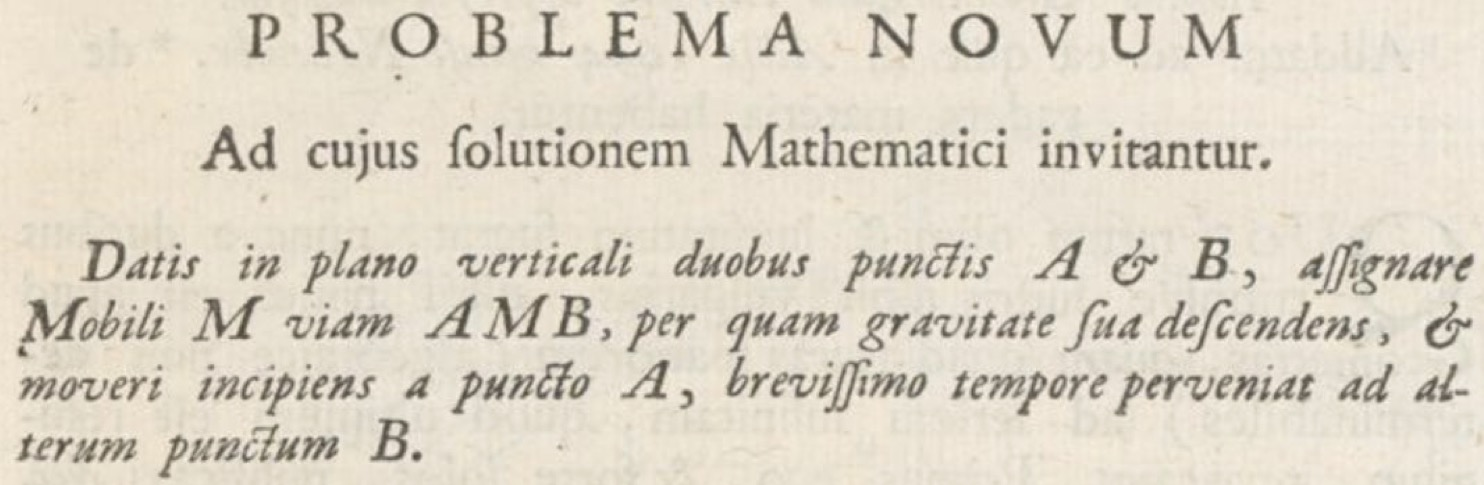
\includegraphics[width=0.8\textwidth]{chapters/020-variation/images/latein.jpg}
\end{center}
Zu deutsch:
\begin{quote}
Neue Aufgabe, zu deren Lösung die Mathematiker eingeladen werden.
Gegeben zwei Punkte $A$ und $B$ in einer vertikalen Ebene, finde
die Bahn $AMB$ eines Punktes $M$, der unter der Wirkung seines
Gewichtes in kürzester Zeit vom Punkt $A$ zum anderen Punkt $B$ absteigt.
\end{quote}
Die Situation der Aufgabenstellung ist in
Abbildung~\ref{buch:variation:fig:brachistochronenproblem}
dargestellt.
Bernoulli hat als Lösung gefunden, dass die Kurve eine Ausschnitt
aus einer Zykloide (in der Abbildung grau) sein muss.
Seine Lösung beruhte auf der Beobachtung, dass sich das Problem analog
zu einem Lichtausbreitungsproblem ist, für welches Fermat bereits
eine Lösung gefunden hat.

Da die Reibung vernachlässigt wird, ist die Energie des Massepunktes
erhalten.
Sie setzt sich aus der potenziellen und der kinetischen Energie
zusammen.
Die potenzielle Energie ist $-mgy$, die kinetische Energie ist
$\frac12mv^2$.
Die Energieerhaltung wird daher zu
\[
E=\frac12mv^2-mgy
\qquad\Rightarrow\qquad
v
=
\sqrt{2g}\!\sqrt{\frac{E}{gm}+y}
=
\!\sqrt{2(C+y)}.
\]
Durch Wahl einer anderen Zeiteinheit kann die Gleichung noch weiter
vereinfacht zu
\(
v = \sqrt{C+y}
\)
vereinfacht werden.
Gesucht ist also die zeitlich kürzeste Bahn eines Teilchens, 
dessen Geschwindigkeit auf bekannte Art $v(y)$ von der vertikalen
Koordinate abhängt.

%
% Das Fermat-Problem
%
\subsection{Das Fermat-Prinzip}
Bereits Fermat hat erkannt, dass das Brechnungsgesetz von Snellius
als Lösung eines Extremalproblems verstanden werden kann.

\begin{satz}[Fermat]
Sie $c/n_i$ die Geschwindigkeit, mit der sich Licht im Medium $M_i$
ausbreitet.
Ein Lichtstrahl von $A_1$ nach $A_2$ geht durch denjenigen Punkt $B$ 
auf der Grenzfläche zwischen den Medien, für den sich die Sinus der
Winkel $\alpha_i$ zwischen den Strahlen und der Normalen zur Grenzfläche
umgekehrt wie die $n_i$ verhalten, wenn also das Brechungsgesetz
\[
\frac{\sin\alpha_1}{\sin\alpha_2}
=
\frac{n_2}{n_1}
\]
gilt.
\end{satz}

\begin{proof}
Ohne der Beschränkung der Allgmeinheit können wir auf die Betrachtung
einer Ebene beschränken, die die beiden Punkte $A_i$ enthält und senkrecht
auf der Grenzfläche steht.
Wir dürfen weiter annehmen, dass die $x$-Achse in der Grenzfläche liegt 
und die Punkte $A_i$ die Koordinaten $(x_i,y_i)$ und der Punkt $B$ die
Koordinaten $(x,0)$ hat.
Es ist derjenige Punkt $x$ zu bestimmen, für den die Lichtzeit entlang 
des Pfades $A_1BA_2$ minimal wird.
Diese Zeit ist
\begin{align*}
t
&=
\frac{\overline{A_1B}}{c/n_1}
+
\frac{\overline{BA_2}}{c/n_2}
\\
ct
&=
n_1\overline{A_1B}
+
n_2\overline{A_2B}
\\
&=
n_1\!\sqrt{(x-x_1)^2 + y_1^2}
+
n_2\!\sqrt{(x_2-x)^2 + y_2^2}
\end{align*}
Das Minimum wird bei einer Nullstelle der Ableitung nach $x$ gefunden,
also bei einer Lösung der Gleichung
\begin{align*}
0
&=
n_1\frac{2(x_1-x)x}{\sqrt{(x_1-x)^2+y_1^2}}
+
n_2\frac{-2(x-x_2)x}{\sqrt{(x_2-x)^2+y_2^2}}.
\intertext{Indem man den zweiten Term auf der rechten Seite auf die linke
Seite bringt und durch $x$ dividiert, erhält man}
n_1
\frac{x_1-x}{\sqrt{(x_1-x)^2+y_1^2}}
&=
n_2
\frac{x-x_2}{\sqrt{(x_2-x)^2+y_2^2}}.
\end{align*}
Der Nenner ist auf beiden Seiten die Hypothenuse eines rechtwinkligen
Dreiecks, welches als Ankathete die Normale zur Grenzfläche hat.
Der Zähler ist die Gegenkathete des Winkels $\alpha_i$ zwischen der
Hypothenuse und der Normalen.
Daher ist der Quotient der Sinus des Winkels oder
\begin{equation}
n_1 \sin\alpha_1 = n_2 \sin\alpha_2.
\label{buch:variation:problem:eqn:snelliusinvariante}
\end{equation}
Die Gleichung~\eqref{buch:variation:problem:eqn:snelliusinvariante}
ist gleichbedeutend mit dem Brechungsgesetz
\[
\frac{\sin\alpha_1}{\sin\alpha_2}
=
\frac{n_2}{n_1}
\]
von Snellius.
\end{proof}

Der Satz von Fermat etabliert das Brechungsgsetz also Lösung eines
Extremalproblems.
Die Natur wählt für einen Lichtstrahl den zeitlich kürzesten Weg.
Der Beweis des Satzes von Fermat zeigt, dass entlang des Lichtstrahls
an jeder Grenzfläche zwischen Medien die Bedingung
\eqref{buch:variation:problem:eqn:snelliusinvariante}
erfüllt.
Wenn die optische Dichte $n$ eine Funktion von $n(y)$ ist, dann
wird der Lichtstrahl nicht nur in diskreten Punkten geknickt, sondern
entlang des ganzen Strahles gekrümmt.
Folgt der Strahl der Kurve $x(y)$, die mit der vertikalen den Winkel
$x'(y) = \tan\alpha(y)$ einschliesst.
Damit lässt sich auch die Sinus-Funktion ausdrücken, es gilt
\[
\sin\alpha(y)
=
\frac{x'(y)}{\pm\!\sqrt{x'(y)^2+1}}.
\]
Aus der Form~\eqref{buch:variation:problem:eqn:snelliusinvariante}
des Brechungsgesetztes wird dann die Gleichung
\begin{equation}
n_1\sin\alpha(y)
=
\frac{n_1(y)x'(y)}{\pm\!\sqrt{x'(y)^2+1}}
=
\operatorname{const}
\qquad\Rightarrow\qquad
\frac{n_1(y)^2x'(y)^2}{x'(y)^2+1}=C.
\label{buch:variation:eqn:fermatdgl}
\end{equation}
Dies ist eine Differentialgleichung für die Funktion $x(y)$.
Sie kann auch in die Form
\[
x'(y)^2
=
\frac{C}{(n_1(y)^2-C)}
\]
gebracht werden.

%
% Das Brachistochronenproblem als Lichtausbreitungsproblem
%
\subsubsection{Das Brachistochronenproblem als Lichtausbreitungsproblem}
Das Fermat-Prinzip besagt, dass ein Lichtstrahl, der sich in einem Medium
mit der Geschwindigkeit $c/n(y)$ ausbreitet, die Gleichung 
\eqref{buch:variation:eqn:fermatdgl} erfüllt.
Beim Brachistochronenproblem ist die Geschwindigkeit $v(y)=\!\sqrt{C-y}$ und 
damit $n(y) = c/\!\sqrt{C-y}$.
Eine Brachistochrone ist also eine Kurve, die die aus
\eqref{buch:variation:eqn:fermatdgl} folgende Gleichung
\begin{equation}
\frac{x'(y)^2}{(1+x'(y)^2)(C-y)} = K
\label{buch:variation:problem:eqn:bernoullidgl}
\end{equation}
erfüllen.

%
% Die Bernoullische Lösung
%
\subsubsection{Die Bernoullische Lösung}
Bernoulli hat gefunden, dass die Brachistochrone ein Zykloidenbogen ist.
Dies lässt sich dadurch verifizieren, dass man die Parametrisierung
einer Zykloide in die
Gleichung~\eqref{buch:variation:problem:eqn:bernoullidgl}
einsetzt.
Die Zykloide hat die Parametrisierung
\[
\left.
\begin{aligned}
x &= r(\varphi - \sin\varphi) 
\\
y &= r(1-\cos\varphi)
\end{aligned}
\right\}
\quad
\text{mit der Ableitung}
\quad
\left\{
\begin{aligned}
\dot{x}(\varphi) &= r(1-\cos\varphi)\\
\dot{y}(\varphi) &= r\sin\varphi
\end{aligned}
\right.
\]
für $\varphi\in\mathbb{R}$.
Die Ableitung ist
\[
x'(y)
=
\frac{\dot{x}(\varphi)}{\dot{y}(\varphi)}
=
\frac{1-\cos\varphi}{\sin\varphi}.
\]
Eingesetzt in \eqref{buch:variation:problem:eqn:bernoullidgl}
wird daraus
\[
\frac{\dot{x}(\varphi)^2}{
(\dot{y}(\varphi)^2 +\dot{x}(\varphi)^2)
(C-r(1-\cos\varphi))
}
=
\frac{(1-\cos\varphi)^2}{
((1-\cos\varphi)^2+\sin^2\varphi)
(C-r+r\cos\varphi)
}
=
K.
\]
Ausmultiplizieren im Nenner ergibt
\[
\frac{(1-\cos\varphi)^2}{
(1-2\cos\varphi+\cos^2\varphi+\sin^2\varphi)
(C-r+r\cos\varphi)
}
=
\frac{1-\cos\varphi}{
2(C-r+r\cos\varphi)
}
\]

%
% Das Brachistochronenproblem als Variationsproblem
%
\subsection{Das Brachistochronenproblem als Variationsproblem
\label{buch:variation:problem:subsection:variationsproblem}}
Die Bernoullische Lösung des Brachistochronenproblems verwendet die
Analogie zum Fermat-Prinzip.
Eine solche Analogie ist nur selten möglich, daher soll das Problem
jetzt in eine Form gebracht werden, in die auch viele ähnliche
Optimierungsproblem gebracht werden können.

Wir erinnern daran, dass die Geschwindigkeit des Massepunktes durch
$v(y)=\sqrt{C-y}$ gegeben ist.
Damit lässt sich die Zeit berechnen, die der Massepunkt entlang der
Lösungskurve braucht, wenn man diese als Funktion $y(x)$ mit beschreibt.
Die Punkte $A$ und $B$ sollen die $x$-Koordinaten $a$ bzw.~$b$ haben.
Für das Kurvenstück zwischen den $x$-Koordinaten $x$ und $x+\Delta x$
braucht der Massepunkt die Zeit
\[
\frac{ \sqrt{\Delta x^2 + \Delta y^2} }{v(y)}
=
\frac{ \sqrt{1 + y'(x)^2} }{ v(y) } \Delta x.
\]
Die Zeit ist das Integral
\begin{equation}
t
=
\int_a^b \frac{\sqrt{1+y'(x)^2}}{v(y(x))}\,dx
=
\int_a^b \sqrt{\frac{1+y'(x)^2}{C-y(x)}}\,dx.
\label{buch:variation:problem:eqn:brachint}
\end{equation}
Der Integrand auf der rechten Seite hängt nur von den Funktion $y(x)$
und $y'(x)$ ab.
Dies kommt vor allem daher, dass die Geschwindigkeit nur von $y$ abhängt,
nicht auch noch von $x$.
Im Allgemeinen wird man also davon ausgehen müssen, dass der Integrand
auch noch von $x$ abhängt.
Die Variationsrechnung befasst sich mit Problemen, in denen Funktionen
gefunden werden müssen, die ein Integral wie das in
\eqref{buch:variation:problem:eqn:brachint}
minimiert oder maximiert werden müssen.

\begin{definition}[Lagrange-Funktion des Brachistochronenproblems]
Die Lagrange-Funk\-tion des Brachistochronenproblems ist der
Integrand des Integrals
\eqref{buch:variation:problem:eqn:brachint},
\index{Lagrange-Funktion}%
also die Funktion
\[
L(x,y,y')
=
\sqrt{\frac{1+y^{\prime 2}}{C-y}}.
\]
\end{definition}

%
% Funktionale
%
\subsection{Funktionale
\label{buch:variation:problem:subsection:funktionale}}
Die Variationsrechnung löst Optimierungsproblem, die von einer
Funktion abhängen.
Um dies mathematisch präzis zu fassen, ist zunächst nötig, die Menge
der in Frage kommenden Funktionen so einzuschränken, dass die interessierende
Grösse überhaupt wohldefiniert ist.

%
% Vektorräume
%
\subsubsection{Vektorräume}
Zunächst sind die gemeinsamen algebraischen Eigenschaften zu charakterisieren,
die wir von den für unsere Untersuchungen zweckmässigen Funktionenmengen
erwarten.

\begin{definition}[Vektorraum]
Ein Vektorraum über den reellen Zahlen $\mathbb{R}$ ist einem Menge $V$ mit
zwei Operationen, der Addition und der Multiplikation mit Skalaren
\begin{align*}
    +\colon V\times V         &\to V : (u,v)\mapsto u+v
&
\cdot\colon \mathbb{R}\times V&\to V : (\lambda,v) \mapsto\lambda v
\end{align*}
mit den folgenden Eigenschaften.
\begin{enumerate}
\item
Es gelten die Assoziativgesetze
\begin{align*}
(u+v)+w&=u+(v+w)&&\text{für alle $u,v,w\in V$}\\
(\lambda \mu)v&=\lambda(\mu v)&&\text{für alle $\lambda,\mu\in\mathbb{R},\;v\in V$.}
\end{align*}
\item
Es gibt einen Vektor $0\in V$ mit der Eigenschaft $0+v=v$ für alle
Vektoren $v\in V$.
\item
Zu jedem Vektor $v\in V$ gibt es den entgegengesetzten Vektor $-v\in V$
mit der Eigenschaft, dass $-v+v=0$ ist.
\item
Die Addition von Vektoren ist kommutativ: $u+v=v+u$ für alle $u,v\in V$.
\item
Es gelten die Distributivgesetze 
\begin{align*}
(\lambda + \mu) v &= \lambda v + \mu v
	&\quad\text{für alle $\lambda,\mu\in\mathbb{R},\;v\in V$}\\
\lambda(u+v)      &= \lambda u + \lambda v
	&\quad\text{für alle $\lambda\in\mathbb{R},\;u,v\in V$}
\end{align*}
\end{enumerate}
\end{definition}

Die Mengen $\mathbb{R}^n$ erfüllen die genannten Eigenschaften, sind
also Vektorräume.
Die Definition eines Vektorraums ist aber viel allgemeiner, insbesondere
gehören dazu auch Mengen von Funktionen.
Damit wird es möglich, die Berechnungen in $\mathbb{R}^n$ auf Funktionen
auszudehnen.
Zum Beispiel bilden die stetigen Funktionen auf einem Intervall einen
Vektorraum, wie das folgende Beispiel zeigt.

\begin{beispiel}
Die Menge
\[
C([a,b])
=
\{f\colon[a,b]\to\mathbb{R}\mid \text{$f$ ist stetig}\}
\]
der stetigen Funktionen bildet einen Vektorraum.
Die Operationen sind die punktweise Addition von Funktionen und die
Multiplikation der Werte mit Skalaren, für $f,g\in C([a,b])$ und
$\lambda\in \mathbb{R}$ ist
\begin{align*}
(f+g)(x) &= f(x)+g(x)
&&\text{und}&
(\lambda f)(x) &= \lambda f(x).
\end{align*}
Entscheidend ist, dass die Addition von Funktionen und die Multiplikation
mit Skalaren nicht aus der Menge herausführt.
Tatsächlich wird in der Analysis gezeigt, dass die Summe stetiger Funktionen
wieder stetig ist und dass die Funktion $x\mapsto \lambda f(x)$ stetig,
wenn $f$ stetig ist.
Die übrigen Eigenschaften sind ebenfalls erfüllt, da sie bereits für die
Funktionswerte erfüllt sind.
\end{beispiel}

%
% Norm und Grenzwerte
%
\subsubsection{Norm und Grenzwerte}
Um Analysis zu betreiben, muss man ausdrücken können, dass eine Folge
von Funktionen konvergiert.
Dazu ist ein Abstandsbegriff zwischen Funktionen nötig.

\begin{definition}[Norm, normierter Raum]
Eine {\em Norm} auf einem Vektorraum $V$ ist eine Abbildung
\index{Norm}%
$\|\cdot\|\colon V\to\mathbb{R}^+_0$ mit nichtnegativen reellen Werten
und den folgenden Eigenschaften
\begin{itemize}
\item Definitheit: $\|v\|\ge 0$ für $v\in V$ mit Gleichheit 
genau dann, wenn $v=0$.
\index{Definitheit}%
\item Absolute Homogenität: Für alle Vektoren $v\in V$ und
\index{Homogenität}%
$\lambda\in\mathbb{R}$ gilt $\|\lambda v\| = |\lambda|\, \|v\|$.
\item Dreiecksungleichung: für alle Vektoren $u,v\in V$ gilt
\index{Dreiecksungleichung}%
$\|u+v\|\le \|u\|+\|v\|$.
\end{itemize}
Ein {\em normierter Raum} ist ein Vektorraum mit einer Norm.
\index{normierter Raum}%
\end{definition}

\begin{beispiel}
Der Vektorraum der stetigen Funktionen kann mit der Supremum-Norm
\[
\|f\| = \sup_{x\in[a,b]} |f(x)|
\]
zu einem normierten Raum gemacht werden.
Die Definitheit ist durch die Definition offensichtlich sichersgtellt.
Für $\|\lambda f\|$ finden wir
\[
\|\lambda f\|
=
\sup_{x\in[a,b]} |\lambda f(x)|
=
|\lambda|\,
\sup_{x\in[a,b]} |f(x)|
=
|\lambda|\, \|f\|,
\]
was die Homogenität zeigt.
Die Dreiecksungleichung folgt aus
\begin{align*}
\|f+g\|
&=
\sup_{x\in[a,b]} |f(x)+g(x)|
\\
&\le
\sup_{x\in[a,b]} (|f(x)|+|g(x)|)
\\
&\le
\sup_{x\in[a,b], y\in[a,b]} (|f(x)|+|g(y)|)
\\
&=
\sup_{x\in[a,b]} |f(x)|
+
\sup_{y\in[a,b]} |g(y)|
=
\|f\| + \|g\|.
\qedhere
\end{align*}
\end{beispiel}

Mit einer Norm ist es jetzt möglich, die Konvergenz von Folgen und den
Begriff des Grenzwertes zu definieren.

\begin{definition}[Cauchy-Folge, Grenzwert]
Eine Folge $(x_n)_{n\in\mathbb{N}}$ in $V$ in einem normierten Raum $V$
mit der Norm $\|\cdot\|$
heisst eine Cauchy-Folge, wenn es für jedes $\varepsilon>0$ eine
\index{Cauchy-Folge}%
$N\in \mathbb{N}$ gibt derart, dass
\[
\| x_n - x_m \| < \varepsilon
\quad\forall n,m\ge N.
\]
Der Vektor $x\in V$ heisst {\em Grenzwert} der Folge $(x_n)_{n\in\mathbb{N}}$,
\index{Grenzwert}%
wenn es zu jedem $\varepsilon > 0$ ein $N\mathbb{N}$ gibt derart, dass
\[
\|x_n-x\| < \varepsilon 
\quad\forall n\ge N.
\]
Die Folge $(x_n)_{n\in\mathbb{N}}$  in $V$ heisst {\em konvergent}, wenn
\index{konvergent}%
$x$ der Grenzwert von $(x_n)_{n\in\mathbb{N}}$ ist.
\end{definition}

Der durch die Supremum-Norm definierte Konvergenzbegriff ist die gleichmässige
Konvergenz.
Zur Erinnerung:
Eine Folge $f_n$ von Funktionen heisst gleichmässig konvergent gegen die
Funktion $f$, wenn es zu jedem
$\varepsilon >0$ ein $N\in\mathbb{N}$ gibt derart, dass
\[
|f_n(x) - f(x)|<\varepsilon\quad\forall n>N\text{ und }x\in [a,b].
\]
Die Supremum-Norm ist
\[
\|f_n(x) - f(x)\|
=
\sup_{x\in[a,b]} |f_n(x)-f(x)| < \varepsilon
\]
für alle $n>N$.
Dies ist genau die Konvergenz in der Norm $\|\cdot\|$.
Aus der Analysis ist bekannt, dass eine gleichmässig konvergente 
Funktionenfolge gegen eine stetige Funktion konvergiert.

\begin{definition}[Banach-Raum]
Ein normierter Raum $V$ heisst ein {\em Banach-Raum},
\index{Banach-Raum}%
wenn jede Cauchy-Folge in $V$ einen Grenzwert hat.
\end{definition}

\begin{beispiel}
Die Menge $C^1([0,2])$
der stetigen Funktionen auf dem Intervall $[0,2]$ ist ein normierter
Raum mit der Norm
\[
\|f\|_1
=
\int_0^2 |f(x)|\,dx,
\]
die auch die $L^1$-Norm heisst.
\index{L1-Norm@$L^1$-Norm}%
Zunächst ist nachzuprüfen, dass dies tatsächlich eine Norm ist.
Die Definitheit und die Homogenität von $\|\cdot\|_1$ ist klar, nur
die Dreiecksungleichung erfordert etwas Arbeit.
Für Funktionen $f,g\in L^1([0,2])$ gilt
\begin{align*}
\|f+g\|_1
&=
\int_0^2 |f(x)+g(x)|\,dx
\\
&\le 
\int_0^2 |f(x)|+|g(x)|\,dx
=
\int_0^2 |f(x)|\,dx
+
\int_0^2 |g(x)|\,dx
=
\|f\|_1+\|g\|_1,
\end{align*}
was die Dreeicksungleichung beweist.

Eine Cauchy-Folge in der $L^1$-Norm muss aber nicht unbedingt einen
stetigen Grenzwert haben.
Die Funktionen
\(
f_n(x) =
\begin{cases}
x^n&\quad x< 1\\
1&\quad x\ge 1
\end{cases}
\)
haben die $L^1$-Norm
\begin{align*}
\|f_n-f_m\|_1
=
\int_0^2 |f_n(x)-f_m|\,dx
\\
&=
\biggl|\int_0^1 x^n-x^m\,dx\biggr|
=
\biggl[
\biggl|
\frac{1}{n+1}x^{n+1}
-
\frac{1}{m+1}x^{m+1}
\biggr|
\biggr]_0^1
\\
&=
\biggl|
\frac{1}{n+1}
-
\frac{1}{m+1}\biggr|.
\end{align*}
Wegen
\[
\|f_n-f_m\|_1
<\varepsilon
\]
für $n,m>2/\varepsilon$ ist $f_n$ eine Cauchy-Folge in $L^1$.
In $L^1$ konvergiert die Folge $f_n$ gegen die Funktion
\[
f(x)
=
\begin{cases}
0&\quad x< 1\\
1&\quad x\ge 1.
\end{cases}
\]
Diese Funktion ist aber nicht stetig, da sie bei $x=1$ einen
Sprung hat.
Bezüglich der $L^1$-Norm ist $C^1([a,b])$ als im Allgemeinen
kein Banach-Raum.
\end{beispiel}

%
% Stetige und differenzierbare Funktionen
%
\subsubsection{Stetige und differenzierbare Funktionen}
Mit der Norm lässt sich auch die Stetigkeit von Abbildungen zwischen
normierten Räumen definieren.

\begin{definition}[Stetigkeit]
Eine Funktion $f\colon U\to V$ zwischen normierten Räumen heisst
{\em stetig im Punkt} $x\in U$, wenn es zu jedem $\varepsilon > 0$
\index{stetig in einem Punkt}%
ein $\delta > 0$
gibt derart, dass
\(
\|f(x)-f(y)\| < \delta
\)
wenn
\(
\|x-y\|<\varepsilon
\).
Eine Funktion $f\colon U\to V$ heisst {\em stetig}, wenn sie in
jedem Punkt von $U$ stetig ist.
\end{definition}

Das Bild einer Folge $x_n\in U$, die gegen $x_0\in U$ konvergiert,
ist eine Folge $f(x_n)$ in $V$.
Man sagt, $y\in V$ sei der Grenzwert von $f(x)$ für $x\to x_0$,
wenn $f(x_n)$ für jede solche Folge $x_n$ gegen $y$ konvergiert.
Der Grenzwert wird auch
\[
\lim_{x\to x_0} f(x)
=
y
\]
geschrieben.
Stetige Funktionen zeichnen sich wie in der Analysis der Funktionen
einer Variablen dadurch aus, dass der Grenzwert der Werte der Funktion
auf einer konvergenten Folge mit dem Funktionswert des Grenzwertes
übereinstimmt.

\begin{satz}
Eine Funktion $f\colon U\to V$ ist genau dann stetig im Punkt $x\in U$,
wenn für jede Folge $x_n$ in $U$ mit Grenzwert $x$ die Folge $f(x_n)$
konvergent ist und
\[
\lim_{n\to\infty} f(x_n) = f(x).
\]
Eine lineare Funktion $f\colon U\to V$ ist genau dann stetig,
wenn für jede Nullfolge $x_n$ in $U$ 
\[
\lim_{n\to \infty} f(x_n) = 0
\]
gilt.
\end{satz}

\begin{definition}
Eine Funktion $f\colon U\to V$ zwischen normierten Räumen heisst
differenzierbar im Punkt $x\in U$ wenn es eine lineare Funktion
$Df(x_0)\colon U\to V$ gibt derart, dass
\[
f(x+v) =f(x) + Df(x_0)\cdot v + o(v),
\]
wobei $o(v)$ bedeutet, dass für diese Funktion
\[
\frac{o(v)}{|v|}\to 0
\quad\text{für $v\to 0$}
\]
gilt.
\end{definition}

Funktionen auf einem Vektorraum mit reellen Werten weren auch
{\em Funktionale} genannt.
\index{Funktional}
Vor dem 20.~Jahrhundert wurde häufig ein Untersschied zwischen
Funktionen von endlich vielen reellen Variablen und Funktionen
von einem unendlichdimensionalen Vektorraum gemacht.
Die Entwicklungen dieses  Abschnittes haben gezeigt, dass eine
solche Unterscheidung nicht gerechtfertigt ist.
Es ist lediglich notwendig, die Definitionen allgemein genug zu
fassen und sich jederzeit über die Funktionenmenge und die zu
verwendende Norm Rechenschaft abzulegen.


%
% 2-fundamtenallemma.tex
%
% (c) 2023 Prof Dr Andreas Müller
%
\section{Das Fundamentallemma
\label{buch:variation:section:fundamentallemma}}
\kopfrechts{Das Fundamentallemma}
Im Fall des endlichdimensionalen Extremalproblems ist aus der
Forderung, dass alle Richtungsableitung verschwinden müssen, 
die Bedingung geworden, dass
\[
v\cdot\grad f = 0
\]
sein muss für alle Vektoren $v\in\mathbb{R}^n$.
Wir haben daraus geschlossen, dass der Gradient $\grad f=0$
sein muss.
Wir hatten dies das endlichdimensionale Fundamentallemma genannt,
wegen $e_k\cdot \grad f = D_kf$ war es eine ziemliche Selbstverständlichkeit.
Bei der Lösung von Variationsproblemen, wo es nicht um endlichdimensionale
Vektoren und das Skalarprodukt, sondern um Funktionen und Integrale
geht, brauchen wir eine ähnliche Aussage für Funktionen.

%
% Positive glatte Funktionen mit kompaktem Träger
%
\subsection{Positive glatte Funktionen mit kompaktem Träger}
Die Aussage des Fundamentallemmas für endlichdimensionale Vektoren 
folgte sofort aus der Tatsache, dass es für jedes $k$ einen Vektor
$e_k$ gibt, der nur in der Koordinaten $k$ von $0$ verschieden ist.
Natürlich gibt es auch Funktionen, die nur in genau einem Punkt
von $0$ verschieden sind.
Eine solche Funktion ist aber im allgemeinen nicht differenzier-
oder integrierbar.
In diesem Abschnitt soll daher gezeigt werden, dass es unendlich
oft stetig differnzierbare Funktionen gibt, die nur in einem beliebig
kleinen vorgegebenen Intervall $\ge 0$ sind.

\begin{definition}[Träger]
Der {\em Träger} einer Funktion $f\colon X\to\mathbb{R}$ ist die Menge
\index{Träger}%
\[
\supp f = \{ x\in X\mid f(x)\ne \}.
\]
\end{definition}

Gesucht ist also eine beliebig oft stetig differenzierbare Funktion,
deren Träger in einem vorgegebenen Intervall $[a,b]$ enthalten ist.
Wir konstruieren so eine Funktion in zwei Schritten.

\input{chapters/020-variation/fig/f.tex}

\begin{satz}
\label{buch:variation:fundamentallemma:satz:glatt}
Die Funktion
\[
f(x)
=
\begin{cases}
e^{-1/x}&\qquad x>0\\
0&\qquad x\le 0
\end{cases}
\]
(siehe auch Abbildung~\ref{buch:variation:fundamentallemma:fig:glatt})
ist beliebig oft stetig differenzierbar.
\end{satz}

\begin{proof}
Es ist klar, dass die Funktion $f$ beliebig oft stetig differenzierbar
ist in jedem Punkt $x\ne 0$.
Es ist also nur nachzuweisen, dass $f(x)$ im Punkt $0$ beliebig
oft stetig differenzierbar ist.

Die ersten drei Ableitungen von $f(x)$ sind
\begin{align}
f'(x) &= \frac{1}{x^2} f(x)
\label{buch:variation:fundamentallemma:eqn:f1}
\\
f''(x) &= \frac{1-2x}{x^4}f(x)
\notag
\\
f'''(x) &= \frac{6x^2-6x+1}{x^6}f(x).
\notag
\end{align}
Daraus lässt sich die Vermutung ableiten, dass
\begin{equation}
f^{(n)}(x)
=
\frac{p_{n-1}(x)}{x^{2n}} f(x)
\label{buch:variation:fundamentallemma:eqn:fabl}
\end{equation}
ist, wobei $p_k(x)$ ein Polynom vom Grad $k$ ist.
Wir beweisen diese Vermutung mit Hilfe von vollständiger Induktion.
Die Induktionsverankerung für die $0$-te Ableitung ist trivial.

Wir nehmen jetzt im Sinne der Induktionsannahme an, dass die $n$-te
Ableitung die Form \eqref{buch:variation:fundamentallemma:eqn:fabl}
hat.
Wir müssen zeigen, dass dann auch $f^{(n+1)}(x)$ diese Form hat.
Dazu berechnen wir
\begin{align}
f^{(n+1)}(x)
&=
\frac{d}{dx}
\frac{p_n(x)}{x^{2n}} f(x)
\notag
\\
&=
\frac{p_n'(x)}{x^{2n}} f(x)
-2n
\frac{p_n(x)}{x^{2n+1}} f(x)
+
\frac{p_n(x)}{x^{2n}} f'(x).
\notag
\intertext{Mit der ersten Ableitung
\eqref{buch:variation:fundamentallemma:eqn:f1} wird dies zu}
&=
\frac{p_n'(x)}{x^{2n}} f(x)
-2n
\frac{p_n(x)}{x^{2n+1}} f(x)
+
\frac{p_n(x)}{x^{2n}} \frac{1}{x^2}f(x)
\notag
\\
&=
\frac{x^2p_n'(x) -2nxp_n(x)+p_n(x)}{x^{2n+2}} f(x).
\label{buch:variation:fundamentallemma:eqn:induktionsschritt}
\end{align}
Die Ableitung $p_n'(x)$ ist ein Polynom vom Grad $n-1$ und damit
ist $x^2p_n'(x)$ ein Polynom vom Grad $n+1$.
Ebenso ist $xp_n(x)$ ein Polynom vom Grad $n+1$ während
$p_n(x)$ ein Polynom vom Grad $n$ ist.
Der Zähler von
\eqref{buch:variation:fundamentallemma:eqn:induktionsschritt}
ist
\[
p_{n+1}(x)
=
x^2p_n'(x)+(1 -2nx)p_n(x),
\]
ein Polynom vom Grad $n+1$.
Damit ist der Induktionsschritt erfolgreich und die Behauptung betreffend
die Form von $f^{(n)}(x)$ ist bewiesen.

Es ist jetzt nur noch zu zeigen, dass der Grenzwert von $f^{(n)}(x)$
für $x\to 0+$ verschwindet.
Da das Polynom $p_n(x)$ stetig ist, folgt
\[
\lim_{x\to 0}
f^{(n)}(x)
=
\lim_{x\to 0}\frac{p_n(x)}{x^{2n}}f(x)
=
p_n(0) \lim_{t\to\infty} t^{2n} e^{-t}
=
0.
\]
Damit ist die beliebige stetige Differenzierbarkeit an der Stelle
$x=0$ gezeigt.
\end{proof}

Die Funktion $f(x)$ von 
Satz~\ref{buch:variation:fundamentallemma:satz:glatt} 
erfüllt noch nicht die Forderung, dass sie nur in einem vorgegebenen
Intervall von $0$ verschieden ist.

\input{chapters/020-variation/fig/g.tex}

\begin{satz}
\label{buch:variation:fundamentallemma:satz:gab}
Sei $f(x)$ die Funktion von
Satz~\ref{buch:variation:fundamentallemma:satz:glatt}.
Dann ist
\[
g_{a,b}(x)
=
f(x-a) f(b-x)
\]
eine unendlich oft stetig differenzierbare, nichtnegative Funktion mit Träger
$\supp g_{a,b}=(a,b)$.
\end{satz}

Die Funktionen $g_{a,b}(x)$ sind beliebig oft differenzierbar und nur im
Intervall $[a,b]$ von $0$ verschieden und sogar positiv.
Weil sie stetig sind, sind sie auch integrierbar, man kann also das
Integral über $\mathbb{R}$ berechnen und die Funktion damit normieren.
Die neue Funktion
\[
\frac{1}{N}
\tilde{g}_{a,b}(x)
\qquad\text{mit}\;
N
=
\int_{-\infty}^{\infty}g_{a,b}(x)\,dx
=
\int_a^b g_{a,b}(x)\,dx
\]
ist immer noch beliebig oft stetig differenzierbar und hat zusätzlich die
Eigenschaft
\[
\int_{-\infty}^{\infty}
\tilde{g}_{a,b}(x)\,dx
=
\int_a^b
\tilde{g}_{a,b}(x)\,dx
=
1.
\]
Wir formulieren dieses Resultat als Satz.

\begin{satz}
\label{buch:variation:satz:gabeins}
Zu jedem Intervall $[a,b]$ gibt es eine beliebig oft stetig
differenzierbare Funktion $g(x)$, genau das Intervall $[a,b]$
als Träger hat und deren Integral über $[a,b]$ den Wert $1$ hat.
\end{satz}

%
% Das Fundamentallemma
%
\subsection{Das Fundamentallemma}
Mit der Funktion $g_{a,b}(x)$ von
Satz~\ref{buch:variation:fundamentallemma:satz:gab}
lässt sich jetzt das Fundamentallemma in der folgenden Form
leicht beweisen.

\begin{satz}[Fundamentallemma]
\label{buch:variation:fundamentallemma:satz:fundamentallemma}
Wenn für die stetige Funktion $f\colon[a,b]\to\mathbb{R}$ 
\begin{equation}
\int_a^b f(x)\varphi(x)\,dx = 0
\label{buch:variation:fundamentallemma:eqn:fundamentalbed}
\end{equation}
gilt für jede beliebig oft stetig differenzierbare Funktion $\varphi(x)$ 
dann ist $f(x)=0$.
Das Resultat gilt selbst dann, wenn
\eqref{buch:variation:fundamentallemma:eqn:fundamentalbed}
nur für beliebig oft stetig differenzierbare Funktionen $\varphi(x)$ 
gilt, die ausserdem an den Intervallenden verschwinden:
$\varphi(a)=\varphi(b)=0$.
\end{satz}

\begin{proof}
Wir zeigen mit Hilfe eines Widerspruchs, dass es keinen Punkt $x_0\in[a,b]$
geben kann, für den $f(x_0)\ne 0$ ist.
Dazu nehmen wir also an, dass $f(x_0)\ne 0$ ist.
Falls $f(x_0)<0$ ist, ersetzen wir $f$ durch $-f$, 
die Bedingung
\eqref{buch:variation:fundamentallemma:eqn:fundamentalbed}
ändert sich dadurch nicht.
\input{chapters/020-variation/fig/fundamentallemma.tex}
Wir dürfen daher annehmen, dass $f(x_0)>0$ ist
(Abbildung~\ref{buch:variation:fundamentallemma:fig:beweis}).
Da $f$ stetig ist, gibt es ein Intervall $[x_0-\varepsilon,x_0+\varepsilon]$
derart, dass $f(x)> \frac12 f(x_0)$ für
$x\in[x_0-\varepsilon,x_0+\varepsilon]$ gilt.
Dann gilt für das Integral
\[
\int_a^b
f(x)
g_{x_0-\varepsilon,x_0+\varepsilon} (x)
\,dx
>
\frac{f(x_0)}{2}
\int_a^b
g_{x_0-\varepsilon,x_0+\varepsilon} (x)
\,dx
>
0
\]
im Widerspruch zur Bedingung
\eqref{buch:variation:fundamentallemma:eqn:fundamentalbed}.
Der Widerspruch zeigt, dass $f(x)=0$ sein muss.
\end{proof}

%
% Skalarproduktformulierung des Fundamentallemmas
%
\subsection{Skalaproduktformulierung des Fundamentallemmas}
Die Richtungsableitung einer Funktion endlich vieler Variablen 
konnte als Skalarprodukt mit dem Gradienten geschrieben werden und
das Fundamentallemma hat besagt, dass der Gradient verschwindet,
wenn alle Richtungsableitungen verschwinden.
Diese Schlussweise ist auch für Funktionen möglich, wenn man Funktionen
ein Skalarprodukt definieren kann.

\begin{definition}[$L^2$-Skalarprodukt]
Das {\em Skalarprodukt} zweier quadratintegrierbarer Funktion $f$ und $g$
auf dem Intervall $[a,b]$ ist definiert durch
\[
\langle f,g\rangle
=
\int_a^b f(x)g(x)\,dx.
\]
\end{definition}

\begin{satz}[Fundamentallemma, Skalarproduktform]
Wenn für eine stetige Funktion $f\colon[a,b]\to\mathbb{R}$ das Skalarprodukt
\[
\langle f,\varphi\rangle = 0
\]
ist für jede unendlich oft differenzierbare Funktion $\varphi$ auf dem
Intervall $[a,b]$, dann ist $f=0$.
\end{satz}



%
% 3-eulerlagrange.tex
%
% (c) 2023 Prof Dr Andreas Müller
%
\section{Die Euler-Lagrange Differentialgleichung
\label{buch:variation:section:eulerlagrange}}
\kopfrechts{Die Euler-Lagrange Differentialgleichung}
Das Neuartige an der Aufgabenstellung des Brachistochronenproblems
war, dass eine Funktion gesucht war, so dass ein damit gebildetes
Integral eine Minimaleigenschaft erfüllt.
Für die damalige Mathematik war die Aufgabe, eine Funktion zu finden,
nicht neu.
Die Theorie der Differentialgleichungen war bereits entwickelt,
Newton hat die Infinitesimalrechnung ja erfunden, um damit die
Bewegungsgleichungen der Physik zu formulieren und zu lösen.
In einer Differentialgleichung werden Werte und Ableitungen einer
Funktion an einer einzigen Stelle miteinander verbunden.
Etwas salop formuliert sagt die Differentialgleichung in jedem
Punkt, in welche Richtung und mit welcher Krümmung die Funktionskurve
weiter zu zeichnen ist.

Im Brachistochronenproblem tragen aber alle Werte der gesuchten
Funktion zum Integral bei, es scheint daher auf den ersten Blick
nicht möglich, das Problem durch schrittweise Konstruktion
``von Punkt zu Punkt'' der Lösungskurve zu konstruieren.

Bernoullis Lösung des Brachistochrononproblems beruht auf der
Beobachtung, dass sich die Bedinung für die schnellste Bahn
durch eine Bedingung ersetzen lässt, die in jedem einzelnen
Punkt ausgewertet werden kann.
Das von ihm verwendete Fermat-Prinzip wurde ursprünglich ebenfalls
als eine globale Eigenschaft eines Lichtstrahls formuliert.
Aus dem Fermat-Prinzip folgt aber das Brechungsgesetz, welches
sagt, dass die Richtung eines Strahls in einem Punkt genau dann
ändert, wenn sich dort auch der Brechungsindex der beiden Medien
ändert.
Das Fermat-Prinzip ist also ein Beispiel dafür, wie eine globale
Bedingung erfüllt werden kann, indem einer lokalen Regel in jedem
Punkt gefolgt wird.

Es ist das Verdienst von Euler und Lagrange, zu erkennen, dass diese
Übersetzung eines globalen Variationsproblems in ein lokales 
Problem immer möglich ist.
Es entsteht dabei die Euler-Lagrange-Differentialgleichung, welche
die Problemstellung auf die Lösung einer Differentialgleichung
reduziert.
Damit ist ein allgemein anwendbares Lösungsverfahren gefunden.
Zu einem Variationsproblem lässt sich immer eine Differentialgleichung
finden, welche die gesuchte Funktion als Lösung hat.

In diesem Abschnitt soll dieser indirekte Weg der Lösung von
Variationsaufgaben dargestellt werden.
Wir werden später zeigen, dass diese Vorgehensweise nicht immer
erfolgreich sein kann.
Zum Beispiel werden wir in Kapitel~\ref{buch:chapter:nichtdiff}
Variationsprobleme kennenlernen, deren Lösungskurven nicht
differenzierbar sind und daher auch nicht von einer Differentialgleichung
gefunden werden können.
Im Kapitel~\ref{buch:chapter:direkt} werden daher die sogenannten
direkten Methodn vorgestellt, die den Umweg über eine
Differentialgleichung vermeiden.

%
% Die Lagrange-Funktion
%
\subsection{Die Lagrange-Funktion
\label{buch:variation:eulerlagrange:subsection:lagrange-funktion}}
Wir betrachten Variationsproblem der folgenden Art.
Gesucht ist eine auf dem Intervall $[x_0,x_1]$ definirte
Funktion $y(x)$, die das Integral
\begin{equation}
I(y)
=
\int_{x_0}^{x_1}
F(x, y(x), y'(x))
\,dx
\label{buch:variation:eulerlagrange:eqn:funktional}
\end{equation}
maximiert oder minimiert.
Der Ausdruck~\eqref{buch:variation:eulerlagrange:eqn:funktional}
wird ein Funktional genannt.
Die Funktion
\[
F
\colon
\mathbb{R}\times
\mathbb{R}\times
\mathbb{R}
\to
\mathbb{R}
\]
von drei Variablen heisst die {\em Lagrange-Funktion}
des Funktionals \eqref{buch:variation:eulerlagrange:eqn:funktional}.

\begin{beispiel}
Die Lagrange-Funktion des Brachistochronenproblems ist
\[
F(x,y,y')
=
\sqrt{ \frac{1+y^{\prime 2}}{y} }.
\]
Die Funktion hängt nicht von $x$ ab, was bedeutet, dass eine
Verschiebung in $x$-Richtung die Form der Lösungsfunktion des
Variationsproblems nicht ändert.
\end{beispiel}

\begin{beispiel}
\label{buch:variation:eulerlagrange:beispiel:gerade}
Wir formulieren die Aufgabe, die kürzeste Verbindung der Punkte
$(x_0,y_0)$ und $(x_1,y_1)$ in einer Ebene zu finden, als Variationsproblem.
Die Länge einer Kurve $y(x)$ ist das Integral
\[
l(y)
=
\int_{x_0}^{x_1}
\sqrt{1+y'(x)^2}\,dx.
\]
Daraus lesen wir ab, dass die Lagrange-Funktion dieses Variationsproblems
\begin{equation}
F(x,y,y') = \sqrt{1+y^{\prime 2}}
\label{buch:variation:eulerlagrange:eqn:geradeL}
\end{equation}
ist.
Die Funktion hängt weder von $x$ noch von $y$ ab.
Dies ist auch zu erwarten, denn die Länge einer Kurve hängt nicht davon
ob, wo in der Ebene sie platziert ist.
Eine Verschiebung in $x$-Richtung würde das $x$-Argument ändern,
eine Verschiebung in $y$-Richtung die $y$-Werte.
Wäre $F$ von $x$ oder $y$ abhängig, könnte auch die Länge der Kurve
davon abhängen.
\end{beispiel}

%
% Euler-Lagrange_Differentialgleichung
%
\subsection{Euler-Lagrange-Differentialgleichung
\label{buch:variation:eulerlagrange:subsection:dgl}}
\input{chapters/020-variation/fig/variation0.tex}
Das Maximum oder Minimum einer Funktionen mehrere Variablen wurde
gefunden, indem die Richtungsableitung berechnet und $=0$ gesetzt
wurde.
Um die Funktion zu bestimmen, die ein Funktional $I(y)$ zu einem
Maximum oder Minimum macht, versuchen wir, die Idee der Richtungsableitung
für ein Funktional nachzuahmen.
Wir nehmen daher an, dass $y(x)$ eine Funktion ist, die das Funktional
$I(y)$ zu einem Minimum macht.
Für die Richtungsableitung addieren wir ein Vielfaches einer
Funktion $\eta(x)$, die Summe $y(x)+\varepsilon\eta(x)$ entspricht
dann einer Geraden mit Richtung $\eta(x)$ im Funktionenraum
(Abbildung~\ref{buch:variation:fig:variation0}).
Die Funktionen $y(x)+\varepsilon\eta(x)$ sind aber nur dann Kandidaten
für eine Lösung des Problems, wenn immer noch
\begin{align*}
y(x_0) + \varepsilon \eta(x_0) &= y_0
&&\text{und}&
y(x_1) + \varepsilon \eta(x_1) &= y_1
\end{align*}
gilt.
Dies ist nur möglich, wenn $\eta(x_0)=\eta(x_1)=0$ ist.

Wir berechnen jetzt die Ableitung der Funktion
$\varepsilon\mapsto I(y+\varepsilon\eta )$ an der Stelle $\varepsilon=0$.
Da die Intervallgrenzen nicht von $\varepsilon$ abhängen, können wir
die Ableitung unter das Integral nehmen:
\begin{align*}
\frac{d}{d\varepsilon}
I(y+\varepsilon\eta)
&=
\int_{x_0}^{x_1}
\frac{d}{d\varepsilon}
F(x,y(x)+\varepsilon\eta(x),y(x)+\varepsilon\eta'(x))
\,dx.
\intertext{Da $F$ differenzierbar ist, kann die Ableitung mit der
Kettenregel berechnet werden, sie ist}
&=
\int_{x_0}^{x_1}
\frac{\partial F}{\partial y}
(x,y(x)+\varepsilon\eta(x),y(x)+\varepsilon\eta'(x))
\eta(x)
\\
&\qquad
+
\frac{\partial F}{\partial y'}
(x,y(x)+\varepsilon\eta(x),y(x)+\varepsilon\eta'(x))
\eta'(x)
\,dx.
\intertext{Uns interessiert aber nur der Wert an der Stelle $\varepsilon=0$,
er ist}
\frac{d}{d\varepsilon}
I(y+\varepsilon\eta)
\bigg|_{\varepsilon=0}
&=
\int_{x_0}^{x_1}
\frac{\partial F}{\partial y}
(x,y(x),y'(x))
\,
\eta(x)
+
\frac{\partial F}{\partial y'}
(x,y(x),y'(x))
\,
\eta'(x)
\,dx
=0.
\end{align*}
Das Integral hängt von den verschiedenen Faktoren $\eta(x)$ und
von $\eta'(x)$ in den beiden Termen unter dem Integral ab.
Wir integrieren den zweiten Term partiell 
\begin{align*}
\int_{x_0}^{x_1}
\frac{\partial F}{\partial y'}(x,y(x),y'(x))\,\eta'(x)\,dx
&=
\biggl[
\frac{\partial F}{\partial y'}(x,y(x),y'(x))\,\eta(x)
\biggr]_{x_0}^{x_1}
\\
&\qquad
-
\int_{x_0}^{x_1}
\frac{d}{dx}
\frac{\partial F}{\partial y'}(x,y(x),y'(x))\,\eta(x)\,dx.
\end{align*}
Da $\eta(x_0)=\eta(x_1)=0$ verschwindet der erste Term
auf der rechten Seite, es bleibt
\[
\frac{d}{d\varepsilon}
I(y+\varepsilon\eta)
\bigg|_{\varepsilon=0}
=
\int_{x_0}^{x_1}
\biggl(
\frac{\partial F}{\partial y}
(x,y(x),y'(x))
-
\frac{d}{dx}
\frac{\partial F}{\partial y'}
(x,y(x),y'(x))
\biggr)
\eta(x)
\,dx.
\]
Dies kann auch als Skalarprodukt
\[
\biggl\langle 
\frac{\partial F}{\partial y}
(x,y(x),y'(x))
-
\frac{d}{dx}
\frac{\partial F}{\partial y'}
(x,y(x),y'(x))
,
\eta(x)
\biggr\rangle
=
0
\]
geschrieben werden.
Da dies für jede differenzierbare Funktion $\eta$ mit Randwerten
$\eta(x_0)=\eta(x_1)$ gelten muss, folgt nach dem
Fundamentallemma~\ref{buch:variation:fundamentallemma:satz:fundamentallemma},
der folgende Satz. 

\begin{satz}[Euler-Lagrange]
\label{buch:variation:eulerlagrange:satz:eulerlagrange}
Wenn die mindestens zweimal stetig differenzierbare Funktion $y(x)$
unter allen solchen Funktionen mit $y(x_0)=y_0$ und $y(x_1)=y_1$
das Funktional
\[
I(y)
=
\int_{x_0}^{x_1}
F(x,y(x),y'(x))\,dx
\]
zu einem Maximum oder Minimum macht, dann ist $y(x)$ eine Lösung der
gewöhnlichen Differentialgleichung
\begin{equation}
\frac{d}{dx}
\frac{\partial F}{\partial y'}(x,y(x),y'(x))
-
\frac{\partial F}{\partial y}(x,y(x),y'(x))
=
0.
\label{buch:variation:eulerlagrange:eqn:eulerlagrange}
\end{equation}
Sie heisst die {\em Euler-Lagrange-Differentialgleichung}.
\end{satz}

Eine Lösung des Variationsproblems kann also als Lösung der
Euler-Lagrange-Dif\-fe\-ren\-tial\-glei\-chung mit den Randwerten
$y(x_0)=x_0$ und $y(x_1)=y_1$ gefunden werden.
Die Bedingung ist notwendig, aber nicht hinreichend.
Wie bei der Bestimmung eines Extremums bei Funktionen endlich
vieler Variablen garantiert das Verschwinden der Richtungsableitung
nicht, dass auch tatsächlich ein Extremum vorliegt.
Man sagt daher auch, dass eine Lösung $y(x)$ der
Euler-Lagrange-Differentialgleichung das Funktional $I(y)$
stationär macht.

Eine weitere Einschränkung ist, dass die Herleitung der
Euler-Lagrange-Differential\-gleichung vorausgesetzt hat,
dass die Lösungsfunktion $y(x)$ mindestens zweimal 
stetig differenzierbar ist.
Es gibt aber durchaus Variationsprobleme, deren Lösungen
nicht differenzierbar sind, dazu mehr im Kapitel~\ref{buch:chapter:nichtdiff}.

\begin{beispiel}
\label{buch:variation:eulerlagrange:beispiel:gerade}
Wir lösen das Variationsproblem von Beispiel
\ref{buch:variation:eulerlagrange:beispiel:gerade}
mit der Lagrange-Funk\-tion
\eqref{buch:variation:eulerlagrange:eqn:geradeL}.
Da die Lagrange-Funktion nicht von $y$ abhängt, bleibt von der 
Euler-Lagrange-Gleichung nur
\[
\frac{d}{dx}
\frac{\partial L}{\partial y'}(x,y(x),y'(x))
=
0
\]
übrig.
Berechnung der Ableitung liefert
\begin{equation}
\frac{\partial}{\partial y'}
\sqrt{1+y^{\prime 2}}
=
\frac{y'}{\sqrt{1+y^{\prime 2}}}.
\label{buch:variation:eulerlagrange:eqn:ableitungFyp}
\end{equation}
Die Ableitung nach $x$ ergibt
\begin{align*}
\frac{d}{dx}
\frac{\partial}{\partial y'}
\sqrt{1+y^{\prime 2}}
&=
\frac{d}{dx}
\frac{y'}{\sqrt{1+y^{\prime 2}}}
\\
&=
\frac{
y''\sqrt{1+y^{\prime 2}}-y'\cdot \frac{y'y''}{\sqrt{1+y^{\prime 2}}}
}{
1+y^{\prime 2}
}
\\
&=
y''
\frac{
1+y^{\prime 2}-y^{\prime 2}
}{
(1+y^{\prime 2})^{\frac32}
}.
\intertext{Die Euler-Lagrange-Differentialgleichung ist daher}
0
&=
\frac{y''}{(1+y^{\prime 2})^{\frac32}} .
\end{align*}
Der Nenner auf der rechten Seite ist immer $\ge 1$, die Gleichung kann
also nur erfüllt sein, wenn $y''=0$ ist.
Die Funktion $y(x)$ muss also eine lineare Funktion $y=ax+b$ sein.
Die Randbedingung wird erfüllt für die Geradengleichung
\[
y(x)
=
\frac{y_1-y_0}{x_1-x_0}(x-x_0) + y_0.
\]
Kürzeste Verbindungen in der Ebene sind daher Geraden.
\end{beispiel}

%
% Freie Randbedingungen
%
\subsection{Freie Randbedingungen
\label{buch:variation:eulerlagrange:subsection:freierb}}
In der Herleitung der Euler-Lagrange-Differentialgleichung wurde angenommen,
dass die Endpunkte der Lösungsfunktion durch $y(x_0)=y_0$ und $y(x_1)=y_1$
fest vorgegeben sind.
Diese Voraussetzung soll in diesem Abschnitt abgeschwächt werden.
Die Funktionswerte in den Endpunkten sollen also nicht mehr fest
vorgegeben sein.

\begin{beispiel}
\label{buch:variation:eulerlagrange:beispiel:freiegerade}
Im Beispiel~\ref{buch:variation:eulerlagrange:beispiel:gerade}
wurde die kürzeste Kurve zwischen zwei Punkten in der Ebene
gesucht und wie erwartet eine Gerade als Lösung gefunden.
Wenn die Werte $y_0$ und $y_1$ jetzt nicht mehr vorgegeben sind,
wird die kürzeste Verbindung zwischen den beiden Geraden
$x=x_0$ und $x=x_1$ gesucht.
Die Lösung dieses Problems ist nicht eindeutig, jede horizontale
Strecke mit $y_0=y_1$ ist eine Lösung.
\end{beispiel}

Das Beispiel zeigt, dass es im Allgemeinen immer noch die Vorgabe
eines der beiden Randwerte braucht, um die Lösung eindeutig zu
bestimmen.
Wir lösen daher die folgende Aufgabe.

\begin{aufgabe}
Gesucht ist eine zweimal stetig differnzierbare Funktion $y(x)$ auf
dem Intervall $[x_0,x_1]$ mit $y(x_0)=y_0$, die das Integral
\[
I(y)
=
\int_{x_0}^{x_1} F(x,y(x),y'(x))\,dx
\]
zu einem Extremum macht.
Am rechten Ende des Intervalls ist der Funktion $y(x)$ keine
Randbedingung auferlegt.
\end{aufgabe}

\begin{proof}[Lösung]
\input{chapters/020-variation/fig/variation1.tex}
Sei $y(x)$ eine Lösung der Aufgabe und sei $y_1:=y(x_1)$ der Wert
der Lösung am rechten Rand des Intervalls.
Wir berechnen wieder die Variation von $I(y)$ mit Hilfe von
stetig differenzierbaren Funktionen $\eta(x)$, die jetzt aber 
nur noch die Bedingungn $\eta(x_0)=0$ erfüllen müssen
(Abbildung~\ref{buch:variation:fig:variation1}).
Die Richtungsableitung ist wie früher
\begin{align*}
\frac{d}{d\varepsilon}
I(y+\varepsilon\eta)
\bigg|_{\varepsilon=0}
&=
\frac{d}{d\varepsilon}
\int_{x_0}^{x_1}
F(x,y(x)+\varepsilon\eta(x),y'(x)+\varepsilon\eta'(x))\,dx
\\
&=
\int_{x_0}^{x_1}
\frac{\partial F}{\partial y}(x,y(x),y'(x)) 
\eta(x)
+
\frac{\partial F}{\partial y'}
(x,y(x),y'(x))
\eta'(x)
\,dx
\intertext{und mit partieller Integration}
&=
\biggl[
\frac{\partial F}{\partial y'}(x,y(x),y'(x)) \eta(x)
\biggr]_{x_0}^{x_1}
\\
&\qquad
+
\int_{x_0}^{x_1}
\biggl(
\frac{\partial F}{\partial y}(x,y(x),y'(x))
-
\frac{d}{dx}
\frac{\partial F}{\partial y'}(x,y(x),y'(x))
\biggr)
\,
\eta(x)
\,dx.
\end{align*}
Im Gegensatz zu früher können wir jetzt aber nicht mehr
schliessen, dass der erste Term verschwindet, da $y(x_1)$ nicht
mehr als $=0$ verausgesetzt wird.
Vielmehr erhalten wir für die erste Variation
\begin{equation*}
\delta I(y)
=
\frac{\partial F}{\partial y'} (x_1,y(x_1),y'(x_1)) \eta(x_1)+
\int_{x_0}^{x_1}
\biggl(
\frac{\partial F}{\partial y}(x,y(x),y'(x))
-
\frac{d}{dx}
\frac{\partial F}{\partial y'}(x,y(x),y'(x))
\biggr)
\,
\eta(x)
\,dx.
\end{equation*}
Die Klammer im Integral ist von der Euler-Lagrange-Differentialgleichung
her bekannt, aber es ist ein weiterer hinzugekommen, der genau dann
verschwindet wenn auch $\eta(x_1)=0$ ist.

Dann ist $y(x)$ natürlich erst recht eine Lösung des Problems, das
Funktional $I(y)$ mit den {\em zwei} Randbedingungen
$y(x_0)=y_0$ und $y(x_1)=y_1$ zu einem Extremum zu machen, also
muss die Funktion $y(x)$ sicher die Euler-Lagrange-Differentialgleichung
erfüllen.
Die Klammer im Integral wird daher verschwinden, die Variation
reduziert sich auf den ersten Term
\[
\delta I(y)
=
\frac{\partial F}{\partial y'} (x_1,y(x_1),y'(x_1)) \eta(x_1)
=
0.
\]
Sie verschwindet nur dann für alle zulässigen Funktionen $\eta(x)$, wenn
\begin{equation*}
\frac{\partial F}{\partial y'}(x_1,y(x_1),y'(x_1))=0
\end{equation*}
gilt.
Dies ist eine zusätzliche Randbedingung für die Funktion $y(x)$, geschrieben
in einer impliziten Form.
\end{proof}

Wir halten das Resultat der Aufgabenlösung als Satz fest:

\begin{satz}
\label{buch:variation:eulerlagrange:satz:zusaetzlicherb}
Wenn die zweimal stetig differenzierbare Funktion $y(x)$ mit dem
Randwert $y(x_0)=y_0$ das Integral
\[
I(y)
=
\int_{x_0}^{x_1} F(x,y(x),y'(x))\,dx
\]
zu einem Extremum macht, dann erfüllt sie am rechten Intervallende
die Randbedingung
\begin{equation}
\frac{\partial F}{\partial y'}(x_1,y(x_1),y'(x_1))=0.
\label{buch:variation:eulerlagrange:eqn:zusaetzlicherb}
\end{equation}
zusätzlich zur Euler-Lagrange-Gleichung für die Lagrange-Funktion $F$.
\end{satz}

\begin{beispiel}
\label{buch:variation:eulerlagrange:beispiel:einseitigegerade}
Wir betrachten wieder das Funktional
\[
I(y)
=
\int_{x_0}^{x_1}
\sqrt{1+y^{\prime 2}(x)}
\,dx
\]
mit der einzigen Randbedingung $y(x_0)=y_0$, der Funktionswert auf 
der rechten Seite ist nicht vorgebeben.
Der Satz~\eqref{buch:variation:eulerlagrange:satz:zusaetzlicherb}
besagt zunächst, dass die Lösungsfunktion wieder eine Gerade sein
muss, da die Euler-Lagrange-Gleichung erfüllt sein muss.
Zusätzlich muss aber auch die Randbedingung
\eqref{buch:variation:eulerlagrange:eqn:zusaetzlicherb}
am rechten Ende des Intervalls erfüllt sein.
Die Ableitung der Lagrange-Funktion ist in diesem Fall durch
\eqref{buch:variation:eulerlagrange:eqn:ableitungFyp}
gegeben, es muss also
\[
\frac{y'(x_1)}{\sqrt{1+y'(x_1)^2}}
=
0
\qquad\Rightarrow\qquad y'(x_1)=0
\]
gelten.
Die Lösung ist daher wie erwartet eine horizontale Strecke.
\end{beispiel}



%
% 5-hoehereableitungen.tex
%
% (c) 2023 Prof Dr Andreas Müller
%
\section{Höhere Ableitungen
\label{buch:variation:section:hoehereableitungen}}
\kopfrechts{Höhere Ableitungen}
Das Beispiel der Spline-Interpolation in
Abschnitt~\ref{buch:nichtdiff:section:splines}
zeigt, dass es manchmal
nötig ist, höhere Ableitungen als die erste in einem Funktional
zu berücksichtigen.
In diesem Abschnitt wird die Theorie der ersten Variation auf
Funktionale erweitert, die von beliebigen Ableitungen der Funktion $y(x)$
abhängen.

%
% Lagrange-Funktion mit höheren Ableitungen
%
\subsection{Lagrange-Funktion mit höheren Ableitungen}
Die Euler-Lagrange-Differentialgleichung wurde bisher für Funktionale
hergeleitet, deren Lagrange-Funktion von $x$, der Funktion $y(x)$ und
der ersten Ableitung $y'(x)$ abhängen.

\begin{definition}
Eine Funktion $L(x,y,y',\dots,y^{(n)})$ heisst eine Lagrange-Funktion
der Ordnung $n$.
\index{Lagrange-Funktion $n$-ter Ordnung}%
\end{definition}

\begin{beispiel}
Das Variationsproblem für die Spline-Integration hat die Lagrange-Funktion
zweiter Ordnung
\[
L(x,y,y',y'') = y^{\prime\prime 2}
\]
verwendet.
\end{beispiel}

Ein elastischer Stab speichert bei Verbiegung Energie, deren Dichte
entlang des Stabes proportional zur Krümmung ist.
Ist $s\mapsto \gamma(s)\in\mathbb{R}^2$ eine differenzierbare
Parametrisierung einer ebenen Kurve, die die Form eines dünnen elastischen
Stabes beschreibt, dann ist die Gesamtenergie des Stabes bis auf
eine Konstante durch das Integral
\[
E
=
\int_a^b \kappa(s)^2 \,ds
\]
gegeben
Ist $s$ ein Bogenlängenparameter, also $|\dot{\gamma}(s)|=1$, dann ist
die Krümmung die zweite Ableitung, also
\[
I = \int_a^b \ddot{\gamma}(s)^2\,ds.
\]
Diese Parameterdarstellung ist aber nicht die Form, in der wir bis jetzt
Kurven in der Ebene beschreiben konnten.

Sei $y(x)$ eine Funktion, deren Graph einen elastisch verbogenen Stab
in der Ebene beschreibt.
Die Krümmung des Graphen kann nach
\[
\kappa(x)
=
\frac{y''(x)}{(1+y'(x)^2)^{\frac32}}
\]
berechnet werden.
Die Energie des Stabes wird dann
\[
E
=
\int_a^b \frac{y''(x)^2}{(1+y'(x)^2)^3}\,dx.
\]
Die Lagrange-Funktion des Problems der Biegung eines Stabes ist daher
\[
L(x,y,y',y'')
=
\frac{y^{\prime\prime 2}}{(1+y^{\prime 2})^3}.
\]

%
% Die verallgemeinerte Euler-Lagrange-Differentialgleichung
%
\subsection{Die verallgemeinerte Euler-Lagrange-Differentialgleichung}
Auch für ein Variationsproblem mit einer Lagrange-Funktion, die höhere
Ableitungen enthält, lässt sich mit der mehr oder weniger gleichen
Vorgehensweise eine Differentialgleichung für die gesuchte Funktion
$y(x)$ herleiten.
Wie auch im Beispiel zur Spline-Interpolation in
Abschnitt~\ref{buch:nichtdiff:section:splines} angedeutet, wird es
notwendig sein, mehrmals partiell zu integrieren.

Sei also $L(x,y,y',\dots,y^{(n)})$ eine Lagrange-Funktion $n$-ter Ordnung
und sei eine Funktion $y(x)$ gesucht, die ein kritischer Punkt des Funktionals
\[
I(y)
=
\int_a^b L\bigl(x,y(x),y'(x),\dots,y^{(n)}(x)\bigr)\,dx
\]
ist.
Wir berechnen wieder die erste Variation mit Hilfe einer beliebig
oft differenzierbaren Funktion $\eta(x)$, welche in den Endpunkten
des Intervalls zusammen mit allen Ableitungen verschwindet.
Die Variation ist definiert als die Richtungsableitung in Richtung
von $\eta(x)$ als
\begin{align*}
\delta I
&=
\frac{d}{dt}
\int_a^b
L\bigl(x,y(x)+t\eta(x),y'(x)+t\eta'(x),\dots,y^{(n)}(x)+t\eta^{(n)}(x)\bigr)
\,dx\biggl|_{t=0}.
\intertext{Durch Ableitung nach $t$ finden wir}
&=
\int_a^b
\frac{\partial L}{\partial y}\bigl(x,y(x),y'(x),\dots,y^{(n)}(x)\bigr)
\,
\eta(x)
+
\frac{\partial L}{\partial y'}\bigl(x,y(x),y'(x),\dots,y^{(n)}(x)\bigr)
\,
\eta'(x)
\\
&\qquad
+
\dots
+
\frac{\partial L}{\partial y^{(n)}}\bigl(x,y(x),y'(x),\dots,y^{(n)}(x)\bigr)
\,
\eta^{(n)}(x)
\,dx.
\end{align*}
Die Terme mit Ableitungen von $\eta(x)$ können durch partielle
Integration in Terme umgewandelt werden, die nur die Funktion 
$\eta(x)$ enthalten:
\begin{align*}
\delta I
&=
\int_a^b
\frac{\partial L}{\partial y^{(k)}}
\bigl(x,y(x),y'(x),\dots,y^{(n)}(x)\bigr)
\,
\eta^{(k)}(x)
\,dx
\\
&=
\biggl[
\frac{\partial L}{\partial y^{(k)}}
\bigl(x,y(x),y'(x),\dots,y^{(n)}(x)\bigr)
\,
\eta^{(k-1)}(x)
\biggr]_a^b
\\
&\qquad
-
\int_a^b
\frac{d}{dx}
\frac{\partial L}{\partial y^{(k)}}
\bigl(x,y(x),y'(x),\dots,y^{(n)}(x)\bigr)
\,
\eta^{(k-1)}(x)
\,dx.
\intertext{Da die Ableitungen von $\eta(x)$ in den Intervallenden
verschwinden, ist dies gleichbedeutend mit}
&=
-\int_a^b \frac{d}{dx} \frac{\partial L}{\partial y^{(k)}}
\bigl(x,y(x),y'(x),\dots,y^{(n)}(x)\bigr)
\,
\eta^{(k-1)}(x)
\,dx.
\intertext{Durch Iterieren dieser Rechnung erhalten wir}
&=
(-1)^{k}
\int_a^b
\frac{d^k}{dx^k}
\frac{\partial L}{\partial y^{(k)}}
\bigl(x,y(x),y'(x),\dots,y^{(n)}(x)\bigr)
\,
\eta(x)
\,dx.
\end{align*}
Die Variation kann jetzt als
\begin{align*}
\delta I
&=
\int_a^b
\biggl(
\frac{\partial L}{\partial y}
-
\frac{d}{dx}
\frac{\partial L}{\partial y'}
+
\frac{d^2}{dx^2}
\frac{\partial L}{\partial y''}
-
\dots
+
(-1)^n
\frac{d^n}{dx^n}
\frac{\partial L}{\partial y^{(n)}}
\biggr)
\,
\eta(x)
\,dx
\end{align*}
geschrieben werden.
Die Variation $\delta I$ muss für jede Wahl von $\eta(x)$ verschwinden,
daher folgt aus dem Fundamentallemma, dass $y(x)$ die Differentialgleichung
\begin{equation}
\frac{\partial L}{\partial y}
-
\frac{d}{dx}
\frac{\partial L}{\partial y'}
+
\frac{d^2}{dx^2}
\frac{\partial L}{\partial y''}
-
\dots
+
(-1)^n
\frac{d^n}{dx^n}
\frac{\partial L}{\partial y^{(n)}}
=
0
\label{buch:variation:hohere:eqn:eulerlagrange}
\end{equation}
erfüllen muss.
Man beachte, dass wir in dieser Rechnung stillschweigend annehmen,
dass die Funktion $y(x)$ genügend oft stetig differenzierbar ist,
so dass die einzelnen Terme der Differentialgleichung
\eqref{buch:variation:hohere:eqn:eulerlagrange} wohldefiniert sind.

\begin{satz}[Euler-Lagrange-Differentialgleichung]
Eine genügend oft differenzierbare Funktion $y(x)$ ist ein stationärer
Punkt des Integrals
\[
I
=
\int_a^b
L\bigl(x,y(x),y'(x),\dots,y^{(n)}(x)\bigr)
\,dx
\]
mit der Lagrange-Funktion $n$-ter Ordnung $L(x,y,y',\dots,y^{(n)})$,
wenn sie die die Euler-Lagrange-Differentialgleichung
\eqref{buch:variation:hohere:eqn:eulerlagrange} erfüllt.
\end{satz}



%
% 6-mehrerefunktionen.tex
%
% (c) 2023 Prof Dr Andreas Müller
%
\section{Varationsproblem für mehrere Funktionen
\label{buch:variation:section:mehrerefunktionen}}
\kopfrechts{Mehrere Funktionen}
Nur sehr spezielle Kurven können dargestellt werden als Graphen
einer Funktion $y(x)$.
Als Lösung des isoperimetrischen Problems wird ein Kreis erwartet,
der sich sicher nicht so darstellen lässt.
Die natürliche Darstellung eines Kreises ist eine Parameterdarstellung
$t\mapsto(\cos t,\sin t)$, auf die die bisherige Theorie nicht
vorbereitet ist.

%
% Lagrange-Funktion für mehrere Funktionen
%
\subsection{Lagrange-Funktion für mehrere Funktionen
\label{buch:variation:mehrerefunction:subsection:lagrangefunktion}}
Eine Parameterdarstellung einer Kurve ist ein Vektor von Funktionen
$y_1(x),\dots,y_n(x)$.
Wir schreiben auch
\[
y(x)
=
\begin{pmatrix}
y_1(x)\\
\vdots\\
y_n(x)
\end{pmatrix}
\qquad\text{und}\qquad
y'(x)
=
\frac{d}{dx}
\begin{pmatrix}
y_1(x)\\
\vdots\\
y_n(x)
\end{pmatrix}
=
\begin{pmatrix}
y_1'(x)\\
\vdots\\
y_n'(x)
\end{pmatrix}
\]
für die Vektorfunktion und ihre erste Ableitung.

Eine {\em Lagrange-Funktion} für ein Variationsproblem wird von
der unabhängigen Variablen $x$, den Funktionswerten aller Funktionen
$y_1(x),\dots,y_n(x)$ und den Ableitungen $y'_1(x),\dots,y'_n(x)$
abhängen.
Sie ist also eine Funktion von $2n+1$ Variablen, die wir als
\begin{equation*}
F
\colon
\mathbb{R}^{2n+1}\to\mathbb{R}
:
(x,y_1,\dots,y_n,y'_1,\dots,y'_n)\mapsto F(x,y_1,\dots,y_n,y'_1,\dots,y'_n)
\end{equation*}
Mit dieser Schreibweise wird das Funktional, das extremal gemacht 
werden soll.
\[
I(y)
=
\int_{x_0}^{x_1}
F(x,y_1(x),\dots,y_n(x),y'_1(x),\dots,y'_n(x))\,dx.
\]
Der Fall $n=1$ ist der bereits früher behandelte.

Besonders elegant lässt sich die Theorie formulieren, wenn wir
die Lagrange-Funktion als Funktion der vektorwertigen Argumente
$y$ und $y'$ schreiben:
\begin{equation}
F
\colon
\mathbb{R}\times\mathbb{R}^n\times\mathbb{R}^n
\to
\mathbb{R}
:
(x,y,y')
\mapsto F(x,y,y').
\label{buch:variation:mehrerefunktionen:eqn:Fvektor}
\end{equation}
Das zu varierende Integral wird dann
\[
I(y)
=
\int_{x_0}^{x_1}
F(x,y(x),y'(x))
\,dx
\]
In dieser Schreibweise unterscheidet sich das Problem formal
nicht mehr vom bereits behandelten.
Es kann in dieser Form aber nicht mit der bereits hergeleiteten
Euler-Lagrange-Differentialgleichung gelöst werden, da die
Ableitung $\partial F/\partial y$ nach einem Vektor $y$ nicht
definiert ist.

%
% Ableitungen nach den Vektorargumenten
%
\subsection{Ableitungen nach den Vektorargumenten
\label{buch:variation:mehrerefunktionen:subsection:vektorableitung}}
Sei $F$ eine Lagrange-Funktion der Form
\eqref{buch:variation:mehrerefunktionen:eqn:Fvektor}.
Wir möchten die Ableitung nach den Vektorargument $y$ und $y'$ 
definieren, damit wir später im
Abschnitt~\ref{buch:variation:mehrerefunktionen:subsection:eulerlagrange}
die Euler-Lagrange-Gleichungen so kompakt wie möglich schreiben können.

Da der Vektor $y$ aus den Variablen $y_1,\dots,y_n$ besteht und $y'$
aus den $y'_1,\dots,y'_n$, ist jede der Ableitungen
\[
\frac{\partial F}{\partial y_k}
\qquad\text{und}\qquad
\frac{\partial F}{\partial y'_k}
\]
wohldefiniert.
Sie bilden zwei Vektoren, die wir als
\begin{equation}
\frac{\partial}{\partial y}
F(x,y,y')
=
\begin{pmatrix}
\frac{\partial}{\partial y_1}F(x,y,y')\\
\vdots\\
\frac{\partial}{\partial y_n}F(x,y,y')
\end{pmatrix}
\qquad\text{und}\qquad
\frac{\partial}{\partial y'} F(x,y,y')
=
\begin{pmatrix}
\frac{\partial}{\partial y'_1}F(x,y,y')\\
\vdots\\
\frac{\partial}{\partial y'_n}F(x,y,y')
\end{pmatrix}
\end{equation}
schreiben wollen.
Ist $\eta(x)$ eine vektorwertige Funktion mit Komponenten
$\eta_k(x)$, dann kann man jetzt 
die in der Variation von
$f(\varepsilon) = F(x,y(x)+\varepsilon\eta(x),y(x)+\varepsilon\eta(x))$
benötigte Ableitung nach $\varepsilon$ schreiben:
\begin{align*}
\frac{d}{d\varepsilon}f(\varepsilon)
&=
\sum_{k=1}^n
\frac{\partial}{\partial y_k}
F(x,y(x)+\varepsilon\eta(x),y'(x)+\varepsilon\eta'(x))
\eta_k(x)
\\
&\qquad
+
\frac{\partial}{\partial y'_k}
F(x,y(x)+\varepsilon\eta(x),y'(x)+\varepsilon\eta'(x))
\eta_k'(x)
\\
&=
\frac{\partial}{\partial y}
F(x,y(x),y'(x))\cdot \eta(x)
+
\frac{\partial}{\partial y'}
F(x,y(x),y'(x))\cdot \eta'(x)
\end{align*}
Der einzige Unterschied in der Notation gegenüber dem skalaren Fall
ist, dass jeweils das Skalarprodukt zur Multiplikation mit $\eta(x)$
bzw.~$\eta'(x)$ verwendet werden muss.

%
% Die Euler-Lagrange-Differentialgleichung
%
\subsection{Die Euler-Lagrange-Differentialgleichung
\label{buch:variation:mehrerefunktionen:subsection:eulerlagrange}}
Für eine Lagrange-Funktion für $r$ Funktionen $y_1(x),\dots,y_r(x)$
lässt sich die Variation des Integrals
\[
I
=
\int_a^b L(x,y_1(x),y_1'(x),\dots,y_r(x),y_r'(x))\,dx
\]
ganz analog zur einer Lagrange-Funktion
mit nur einer Funktion berechnen.
Dazu verwenden wir Funktionen $\eta_1(x),\dots,\eta_r(x)$, die
in den Endpunkten verschwinden und berechnen die Variation
\begin{align}
\delta I
&=
\frac{d}{dt}
\int_a^b
L(x,y_1(x)+t\eta_1(x),y_1'(x)+t\eta_1'(x),\dots,
y_r(x)+t\eta_r(x),y_r'(x)+t\eta_r'(x))
\,dx
\bigg|_{t=0}
\notag
\\
&=
\int_a^b
\frac{\partial L}{\partial y_1}\eta_1(x)
+
\frac{\partial L}{\partial y'_1}\eta'_1(x)
+
\dots
\frac{\partial L}{\partial y_r}\eta_r(x)
+
\frac{\partial L}{\partial y'_r}\eta'_r(x)
\,dx
\notag
\intertext{Die Terme mit Ableitungen von $\eta'_i(x)$ können durch partielle
Integration umgeformt werden:}
&=
\int_a^b
\frac{\partial L}{\partial y_1}\eta_1(x)
+\dots+
\frac{\partial L}{\partial y_r}\eta_r(x)
\,dx
+
\biggl[
\frac{\partial L}{\partial y'_1}\eta_1(x)
+
\frac{\partial L}{\partial y'_r}\eta_r(x)
\biggr]_a^b
\\
&\qquad
-
\int_a^b
\frac{d}{dx}
\frac{\partial L}{\partial y'_1}
\eta_1(x)
+
\dots
+
\frac{d}{dx}
\frac{\partial L}{\partial y'_r}
\eta_r(x).
\notag
\intertext{Der mittlere Term verschwindet, weil die Funktionen
$\eta_i(x)$ an den Intervallenden verschwinden.
Die Variation ist daher}
\delta I
&=
\int_a^b
\biggl(
\frac{\partial L}{\partial y_1}-\frac{d}{dx}\frac{\partial L}{\partial y'_1}
\biggr)\eta_1(x)
\,dx
+
\dots
+
\int_a^b
\biggl(
\frac{\partial L}{\partial y_r}-\frac{d}{dx}\frac{\partial L}{\partial y'_r}
\biggr)\eta_r(x)
\,dx.
\label{buch:variation:mehrere:eqn:summe}
\end{align}
Da die Funktionen $\eta_i(x)$ alle bis auf eine $=0$ gewählt werden können,
muss jedes der Integrale in \eqref{buch:variation:mehrere:eqn:summe}
verschwinden muss.
Nach dem Fundamentallemma folgt daher der folgende Satz.

\begin{satz}
\label{buch:variation:mehrere:satz:rfunktionen}
Das Integral
\[
\int_a^b L(x,y_1(x),y_1'(x),\dots,y_r(x),y'_r(x))\,dx
\]
mit einer Lagrange-Funktion für $r$ Funktionen $y_1(x),\dots,y_r(x)$
nimmt einen stationären Wert an für Funktionen %$y_1(x),\dots,y_r(x)$,
welche das Differentialgiechungssystem
\begin{equation}
\frac{\partial L}{\partial y_k}(x,y_1(x),y'_1(x),\dots,y_r(x),y'_r(x))
-
\frac{d}{dx}
\frac{\partial L}{\partial y'_k}(x,y_1(x),y'_1(x),\dots,y_r(x),y'_r(x))
=
0,
\label{buch:variation:mehrerefunktionen:eqn:reulerlagrange}
\end{equation}
$k=1,\dots,r$ erfüllen.
\end{satz}

In einen Variationsproblem sind im Allgemeinen geeignete Randbedingungen
notwendig, die die Lösung des Differentialgleichungssystems
\eqref{buch:variation:mehrerefunktionen:eqn:reulerlagrange}
eindeutig festlegen.

%
% Vektorform der Euler-Lagrange-Differentialgleichung
%
\subsubsection{Vektorform der Euler-Lagrange-Differentialgleichung}
Die Lagrange-Funktion $L(x,y_1,y'_1,\dots,y_r,y'_r)$ kann auch als
eine Funktion
\[
L\colon
\mathbb{R}\times\mathbb{R}^r \times \mathbb{R}^r
\to
\mathbb{R}
\]
geschrieben werden.
Die Ableitung $D_2L$ ist die Ableitung nach den Variablen $y_1,\dots,y_r$
während $D_3L$ die Ableitung nach den Variablen $y'_1,\dots,y'_r$ ist.
Gesucht ist wie früher ein stationärer Punkt des Integrals
\[
I
=
\int_a^b L(x,y(x),y'(x))\,dx,
\]
wobei $y\colon[a,b]\to\mathbb{R}^r$ eine vektorwertige Funktion ist.
Um die Variation zu bilden, brauchen wir eine vektorwertige Funktion
$\eta\colon[a,b]\to\mathbb{R}$, deren Komponenten in den Endpunkten
des Intervalls verschwinden.
Die Variation ist dann
\begin{align*}
\delta I
&=
\frac{d}{dx}
\int_a^b L(x, y(x)+t\eta(x), y'(x)+t\eta'(x))\,dx
\bigg|_{t=0}
\\
&=
\int_a^b
D_2L(x,y(x),y'(x)) \eta(x)
+
D_3L(x,y(x),y'(x)) \eta'(x)
\,dx
\intertext{$D_2L$ ist eine Linearform, die auf den Vektor $\eta(x)$ 
angewendet wird, und analog für $D_3L$.
Für den Term mit $\eta'(x)$ verwenden wir wieder partielle Integration}
&=
\int_a^b D_2L(x,y(x),y'(x))\eta(x)\,dx
+
\biggl[L(x,y(x),y'(x))\biggr]_a^b
\\
&\qquad
-
\int_a^b \frac{d}{dx}D_eL(x,y(x),y'(x)) \eta(x)\,dx.
\intertext{Da die Komponenten von $\eta(x)$ an den Intervallenden
verschwinden, fällt der mittlere Term weg und es bleibt}
&=
\int_a^b \bigl(D_2L(x,y(x),y'(x))-\frac{d}{dx}D_3L(x,y(x),y'(x))\bigr)
\eta(x)\,dx.
\end{align*}
Nach dem Fundamentallemma folgt die $r$-dimensionale
Vektor-Differentialgleichung
\[
D_2L(x,y(x),y'(x)) - \frac{d}{dx}D_3L(x,y(x),y'(x)) = 0.
\]
Beide Terme sind Linearformen auf $\mathbb{R}^r$, ihre Koeffizienten
sind die einzelnen Differentialgleichungen von
Satz~\ref{buch:variation:mehrere:satz:rfunktionen}.

%
% Parameterdarstellung von Kurven
%
\subsection{Parameterdarstellung von Kurven
\label{buch:variation:mehrerefunktionen:subsection:kurven}}
Ein Kurve im $r$-dimensionalen Raum $\mathbb{R}^r$ ist eine differenzierbare
Abbildung
\[
\gamma
\colon
\mathbb{R} \to \mathbb{R}^r
:
t \mapsto \gamma(t).
\]
Die Koordinaten von $\gamma(t)$ bilden $r$ Funktionen $\gamma_i(t)$
für $i=1,\dots,r$.
Die Ableitung nach dem Kurvenparameter $t$ ist der Tangentialvektor
\[
\frac{d}{dt}\gamma(t) = \dot{\gamma}(t),
\]
er wird mit dem Punkt bezeichnet.

Ein Variationsproblem für eine Kurve basiert auf einer Lagrange-Funktion
\[
L
\colon
\mathbb{R}\times\mathbb{R}^r\times\mathbb{R}^r
:
(t,x,\dot{x})
\mapsto
L(t,x,\dot{x}),
\]
aus der das Funktional
\begin{equation}
I(\gamma)
=
\int_{t_0}^{t_1}
L(t,\gamma(t),\dot{\gamma}(t))
\,dt
\label{buch:variation:mehrerefunktionen:eqn:funktionalkurve}
\end{equation}
abgeleitet werden kann.
Dies ist natürlich ein Variationsproblem für die $r$ Komponentenfunktionen
des Vektors $\gamma(t)$.

Die Euler-Lagrange-Differentialgleichung für das Funktional
\eqref{buch:variation:mehrerefunktionen:eqn:funktionalkurve}
ist die $r$-dimensionale Vektordifferentialgleichung
\begin{equation}
\frac{\partial L}{\partial x}(t,\gamma(t), \dot{\gamma}(t))
-
\frac{d}{dt}
\frac{\partial L}{\partial \dot{x}}(t,\gamma(t),\dot{\gamma}(t))
=
0.
\label{buch:variation:mehrerefunktionen:eqn:eulerlagrangekurve}
\end{equation}
Zusätzlich sind Randbedingungen notwendig, um die Lösung 
eindeutig festzulegen.
Lösungen der Differentialgleichung
\eqref{buch:variation:mehrerefunktionen:eqn:eulerlagrangekurve}
sind stationäre Punkte des Funktionals
\eqref{buch:variation:mehrerefunktionen:eqn:funktionalkurve}.

%
% Das homogene Problem
%
\subsection{Das homogene Variationsproblem
\label{buch:variation:mehrerefunktionen:subsection:homogen}}







%
% 6-allgemein.tex
%
% (c) 2024 Prof Dr Andreas Müller
%
\section{Die allgemeine Theorie der ersten Variation
\label{buch:variation:section:allgemein}}
\kopfrechts{Die allgemeine Theorie der ersten Variation}
In Abschnitt~\ref{buch:variation:eulerlagrange:subsection:freierb}
wurde gezeigt, wie sich in einem Variationsproblem mit vorgegebenem
Randwert nur an einem Ende des Intervalls aus der ersten Variation
automatisch eine zusätzliche Randbedingung am anderen Ende des
Intervalls ergibt.
Die Endpunkte $x_0$ und $x_1$ des Intervalls waren aber immer noch 
fest.
In diesem Abschnitt soll gezeigt werden, wie sich diese Einschränkung
aufheben lässt.

%
% Allgemeine Variation einer Funktion
%
\subsection{Allgemeine Variation einer Funktion $y(x)$
\label{buch:variation:allgemein:subsection:vary}}
In Abschnitt~\ref{buch:variation:section:eulerlagrange} wurde die
erste Variation mit Hilfe von Funktionen der Form
\begin{equation}
x
\mapsto
y(x)+\varepsilon\eta(x)
\label{buch:variation:allgemein:eqn:ansatz}
\end{equation}
konstruiert.
Mit diesem Ansatz ist es nicht möglich, die Endpunkte $x_0$ und $x_1$
des Intervalls zu varieren.
Es war zwar möglich, die $y$-Werte zu varieren, was auf die zusätzliche
Randbedingung von
Satz~\ref{buch:variation:eulerlagrange:satz:zusaetzlicherb}
geführt hat.
Wir möchten aber sogar die Intervallgrenzen varieren können, dieser
Fall wird von den bisherigen Entwicklungen nicht abgedeckt.

%
% Verallgemeinerung des Variationsansatzes
%
\subsubsection{Verallgemeinerung des Variationsansatzes}
\input{chapters/020-variation/fig/variation.tex}%
Statt des Ansatzes~\eqref{buch:variation:allgemein:eqn:ansatz}
verwenden wir jetzt eine Parametrisierung
\begin{equation}
y
\colon
[x_0(\varepsilon),x_1(\varepsilon)]
\to
\mathbb{R}
:
x\mapsto y(x,\varepsilon)
\label{buch:variation:allgemein:eqn:ansatz2}
\end{equation}
für $\varepsilon$-Werte in einer Umgebung von $0$
(Abbildung~\ref{buch:variation:fig:variation}).
Damit
\eqref{buch:variation:allgemein:eqn:ansatz2}
eine Variation der einer Funktion $y(x)$ beschreibt, soll
$y(x) = y(x,0)$ sein.
Die Funktionen $x_0(\varepsilon)$ und $x_1(\varepsilon)$ beschreiben
die Endpunkte des Definitionsintervalls der partiellen Funktion
$x\mapsto y(x,\varepsilon)$.

Der ursprüngliche Ansatz~\eqref{buch:variation:allgemein:eqn:ansatz}
ist in \eqref{buch:variation:allgemein:eqn:ansatz2} enthalten, wenn
man $x_0(\varepsilon)=x_0$, $x_1(\varepsilon)=x_1$ und
\[
y(x,\varepsilon) = y(x) + \varepsilon \eta(x)
\]
setzt.
In der Herleitung der Euler-Lagrange-Differentialgleichung wurde
entscheidend verwendet, dass man diese Funktion nach $\varepsilon$
ableiten kann.
Dass dies möglich ist, ist nach den bisherigen Forderungen an
$y(x,\varepsilon)$ nicht garantiert.
Es muss also zusätzlich Differenzierbarkeit nach $\varepsilon$
gefordert werden.

\begin{definition}[Allgemeine Variation einer Funktion]
\label{buch:variation:allgemein:def:variation}
Eine stetig nach beiden Variablen differenzierbare Funktion $y(x,\varepsilon)$
ist eine {\em allgemeine Variation} der Funktion $y(x)$, wenn es stetig
differenzierbare Funktionen
$x_0(\varepsilon)$ und $x_1(\varepsilon)$ gibt derart, dass
die partielle Funktion $x\mapsto y(x,\varepsilon)$ auf dem
Intervall $[x_0(\varepsilon),x_1(\varepsilon)]$ stetig differenzierbar
ist und für $\varepsilon=0$ mit $y(x)$ übereinstimmt: $y(x)=y(x,0)$.
Der Einfachheit halber wird die partielle Ableitung von $y(x,\varepsilon)$
nach $x$ auch
\[
y'(x,\varepsilon) = \frac{\partial y}{\partial x}(x,\varepsilon)
\]
geschrieben.
Für die Werte an den Endpunkten schreiben wir abkürzend
\begin{align*}
x_i &= x_i(0),
&
y_i &= y(x_i(0),0) = y(x_i)
&&\text{und}&
y_i'
=
y'(x_i(0),0)
=
\frac{\partial y'(x(\varepsilon),\varepsilon)}{\partial\varepsilon}
\bigg|_{\varepsilon=0}
\end{align*}
für $i=0,1$.
\end{definition}

%
% Kurven, auf denen sich die Endpunkte bewegen
%
\subsubsection{Kurven, auf denen sich die Endpunkte bewegen}
Der Ansatz~\eqref{buch:variation:allgemein:eqn:ansatz2} beschreibt
Kurven, die die beiden Punkte
\begin{align*}
P_0(\varepsilon)
&=
(x_0(\varepsilon),y(x_0(\varepsilon),\varepsilon))
&&\text{und}&
P_1
&=
(x_1(\varepsilon),y(x_1(\varepsilon),\varepsilon))
\end{align*}
miteinander verbinden.
Die Endpunkte der Kurve bewegen sich also auf den Kurven
\begin{align*}
\varepsilon
&\mapsto
P_0(\varepsilon)
=
(x_0(\varepsilon),y(x_0(\varepsilon),\varepsilon)
&&\text{und}&
\varepsilon
&\mapsto
P_1(\varepsilon)
=
(x_1(\varepsilon),y(x_1(\varepsilon),\varepsilon).
\end{align*}
Da alle beteiligten Funktionen als differenzierbar vorausgesetzt wurden,
lassen sich auch die Tangenten dieser Kurven bestimmen.
Der Richtungsvektor der Tangente im Punkt $x_i=x_i(0)$ ist
\begin{align}
\vec{r}_i(\varepsilon)
=
\frac{d}{d\varepsilon}
\begin{pmatrix}
x_i(\varepsilon)\\
y(x_i(\varepsilon),\varepsilon)
\end{pmatrix}
\bigg|_{\varepsilon=0}
\label{buch:variation:allgemein:eqn:tangential}
\end{align}
für $i=0,1$.
Die Kurve $\varepsilon\mapsto P_i(\varepsilon)$ lässt sich daher für
genügend kleine $\varepsilon$ beliebig genau durch
\[
x\mapsto
\begin{pmatrix}
x_0(0)\\
y(x,0) 
\end{pmatrix}
+
\varepsilon
\frac{d}{d\varepsilon}
\begin{pmatrix}
x_i(\varepsilon)\\
y(x_i(\varepsilon),\varepsilon)
\end{pmatrix}
\bigg|_{\varepsilon=0}
\]
approximieren.

%
% Erste Variation
%
\subsection{Erste Variation einer einzelnen Funktion
\label{buch:variation:allgemein:subsection:var1}}
Wir betrachten jetzt wieder das Funktional
\[
I(y)
=
\int_{x_0}^{x_1} F(x,y(x),y'(x)) \,dx
\]
für die Lagrange-Funktion $f(x,y,y')$.
Eine allgemeine Variation der Funktion $y(x)$ im Sinne der
Definition~\ref{buch:variation:allgemein:def:variation} macht aus
$I(y)$ eine Funktion 
\[
I(y,\varepsilon)
=
\int_{x_0(\varepsilon)}^{x_1(\varepsilon)}
F(x,y(x,\varepsilon),y'(x,\varepsilon))
\,dx
\]
von $\varepsilon$.
Davon ist wieder die Ableitung nach $\varepsilon$ an der Stelle
$\varepsilon=0$ zu ermitteln.
Sie ist
\begin{align*}
\frac{\partial}{\partial\varepsilon}I(y,\varepsilon)
&=
F(x_1(\varepsilon),y(x_1(\varepsilon),\varepsilon),
y'(x_1(\varepsilon),\varepsilon))
\frac{dx_1(\varepsilon)}{d\varepsilon}
-
F(x_0(\varepsilon),y(x_0(\varepsilon),\varepsilon),
y'(x_0(\varepsilon),\varepsilon))
\frac{dx_0(\varepsilon)}{d\varepsilon}
\\
&\qquad
+
\int_{x_0(\varepsilon)}^{x_1(\varepsilon)}
\frac{\partial F}{\partial y}(x, y(x,\varepsilon), y'(x,\varepsilon))
\frac{\partial y}{\partial \varepsilon}(x,\varepsilon)
\,dx
\\
&\qquad
+
\int_{x_0(\varepsilon)}^{x_1(\varepsilon)}
\frac{\partial F}{\partial y'}(x, y(x,\varepsilon), y'(x,\varepsilon))
\frac{\partial^2 y}{\partial x\,\partial\varepsilon}(x,\varepsilon)
\,dx
\end{align*}
An der Stelle $\varepsilon=0$ vereinfacht sich die Variation zu
\begin{align}
\delta I(y)
&=
F(x_1,y(x_1),y'(x_1))
\frac{dx_0(0)}{d\varepsilon}
-
F(x_0,y(x_0),y'(x_0))
\frac{dx_1(0)}{d\varepsilon}
\notag
\\
&\qquad
+
\int_{x_0}^{x_1}
\frac{\partial F}{\partial y}(x,y(x),y'(x))
\frac{\partial y}{\partial \varepsilon}(x,0)
\,dx
\notag
\\
&\qquad
+
\int_{x_0}^{x_1}
\frac{\partial F}{\partial y'}(x,y(x),y'(x))
\frac{\partial^2 y}{\partial x\,\partial\varepsilon}(x,0)
\,dx.
\label{buch:variation:allgemein:eqn:var1}
\end{align}
Die Ableitung $y'$ im zweiten Integral kann mit partieller Integration 
vereinfacht werden:
\begin{align*}
\int_{x_0}^{x_1}
\frac{\partial F}{\partial y'}(x,y(x),y'(x))
\frac{\partial y'}{\partial \varepsilon}(x,0)
\,dx
&=
\biggl[
\frac{\partial F}{\partial y'}(x,y(x),y'(x))
\frac{\partial y}{\partial\varepsilon}(x,0)
\biggr]_{x_0}^{x_1}
\\
&\qquad
-
\int_{x_0}^{x_1}
\frac{d}{dx}
\frac{\partial F}{\partial y'}(x,y(x),y'(x))
\frac{\partial y}{\partial\varepsilon}(x,0)
\,dx.
\end{align*}
Eingesetzt in 
\eqref{buch:variation:allgemein:eqn:var1}
ist die allgemeine Variation des Funktionals $I(y)$ daher
\begin{equation}
\begin{aligned}
\delta I(y)
&=
F(x_1,y(x_1),y'(x_1))
\frac{dx_0(0)}{d\varepsilon}
-
F(x_0,y(x_0),y'(x_0))
\frac{dx_1(0)}{d\varepsilon}
\\
&\qquad
+
\biggl[
\frac{\partial F}{\partial y'}(x,y(x),y'(x))
\frac{\partial y}{\partial\varepsilon}(x,0)
\biggr]_{x_0}^{x_1}
\\
&\qquad
+
\int_{x_0}^{x_1}
\biggl(
\frac{\partial F}{\partial y}(x,y(x),y'(x))
-
\frac{d}{dx}\frac{\partial F}{\partial y'}(x,y(x),y'(x))
\biggr)
\frac{\partial y}{\partial \varepsilon}(x,0)
\,dx.
\end{aligned}
\label{buch:variation:allgemein:eqn:variation}
\end{equation}

Sei jetzt $y(x)$ eine Funktion, die das Funktional $I(y)$ stationär macht,
für jede Wahl einer Variation von $y(x)$ ist also $\delta I(y)=0$.
Dies gilt insbesondere auch für alle Variationen, die Endpunkte der
Kurve unverändert lassen.
Für eine solche Variation verschwinden die ersten drei Terme, es bleibt
nur das Integral.
Wie früher folgt daher, dass der Ausdruck in der Klammer im Integral
verschwinden muss.
Eine Lösung des Variationsproblems muss also die
Euler-Lagrange-Differentialgleichung erfüllen.

Die verbleibenden Terme in \eqref{buch:variation:allgemein:eqn:variation}
drücken aus, wie sich das Funktional $I(y)$ ändert, wenn sich die
Endpunkte der Kurve verschieben.
Die ersten zwei Terme behandeln offensichtlich den Fall, dass die 
Intervalgrenzen verschoben werden.
Der dritte Term behandelt die Änderung, die ausschliesslich von der
Änderung des zweiten Parameters von $y(x,\varepsilon)$ ausgeht.
Der $y$-Wert kann sich auch dadurch ändern, dass $x$ variert wird.
\begin{align*}
\frac{dy(x_i(\varepsilon),\varepsilon)}{d\varepsilon}
&=
\frac{\partial y(x_i(\varepsilon),\varepsilon)}{\partial x}
\frac{dx_i(\varepsilon)}{d\varepsilon}
+
\frac{\partial y(x_i(\varepsilon), \varepsilon)}{\partial \varepsilon}
\intertext{oder an der Stelle $\varepsilon=0$}
\frac{dy(x_i(0),0)}{d\varepsilon}
&=
\frac{\partial y(x_i(0),0)}{\partial x}
\frac{dx_i(0)}{d\varepsilon}
+
\frac{\partial y(x_i(0), 0)}{\partial \varepsilon}
\intertext{Aufgelöst nach dem letzten Term ist dies}
\frac{\partial y(x_i(0), 0)}{\partial \varepsilon}
&=
\frac{dy(x_i(0),0)}{d\varepsilon}
-
\frac{\partial y(x_i(0),0)}{\partial x}
\frac{dx_i(0)}{d\varepsilon}
\end{align*}
Dies können wir in die Variation
\eqref{buch:variation:allgemein:eqn:variation}
einsetzen und erhalten
\begin{equation}
\begin{aligned}
\delta I(y)
&=
\biggl(
F(x_1,y(x_1),y'(x_1))
-
\frac{\partial y(x_1(0),0)}{\partial x}
\frac{\partial F}{\partial y'}(x_1,y(x_1),y'(x_1))
\biggr)
\frac{dx_1(0)}{d\varepsilon}
\\
&\qquad
+
\frac{\partial F}{\partial y'}(x_1,y(x_1),y'(x_1))
\frac{dy(x_1(0),0)}{d\varepsilon}
\\
&\qquad
-
\biggl(
F(x_0,y(x_0),y'(x_0))
-
\frac{\partial y(x_0(0),0)}{\partial x}
\frac{\partial F}{\partial y'}(x_0,y(x_0),y'(x_0))
\biggr)
\frac{dx_0(0)}{d\varepsilon}
\\
&\qquad
-
\frac{\partial F}{\partial y'}(x_0,y(x_0),y'(x_0))
\frac{dy(x_0(0),0)}{d\varepsilon}
\\
&\qquad
+
\int_{x_0}^{x_1}
\biggl(
\frac{\partial F}{\partial y}(x,y(x),y'(x))
-
\frac{d}{dx}\frac{\partial F}{\partial y'}(x,y(x),y'(x))
\biggr)
\frac{\partial y}{\partial \varepsilon}(x,0)
\,dx.
\end{aligned}
\label{buch:variation:allgemein:eqn:variation}
\end{equation}
Von den ersten vier Terme lassen sich jeweils zwei als ein Skalarprodukt
des Vektors
\[
\vec{f}_i
=
\begin{pmatrix}
\displaystyle
F(x_i,y(x_i),y'(x_i))
-
\frac{\partial F}{\partial y'}(x_i,y(x_i),y'(x_i))
\frac{\partial y(x_i(0),0)}{\partial\varepsilon}
\\[3pt]
\displaystyle
\frac{\partial F}{\partial y'}(x_i,y(x_i),y'(x_i))
\end{pmatrix}
\]
mit dem Richtungsvektor  $\vec{r}_i(0)$ von
\eqref{buch:variation:allgemein:eqn:tangential} schreiben.
Mit dieser Notation erhält die allgemeinste Form der ersten Variation
die Form
\begin{equation}
\delta I(y)
=
\vec{f}_1\cdot \vec{r}_i(0)
-
\vec{f}_0\cdot \vec{r}_0(0)
+
\int_{x_0}^{x_1}
\biggl(
\frac{\partial F}{\partial y}(x,y(x),y'(x))
-
\frac{d}{dx}\frac{\partial F}{\partial y'}(x,y(x),y'(x))
\biggr)
\frac{\partial y}{\partial \varepsilon}(x,0)
\,dx.
\end{equation}

\begin{satz}[Allgemeine Variationsformel]
\label{buch:variation:allgemein:satz:allgemeinvariation1}
Sei $y(x,\varepsilon)$ eine Variation der zweimal stetig differenzierbaren
Funktion $y(x)$ und sei
\[
\vec{r}_i(0)
=
\frac{d}{d\varepsilon}
\begin{pmatrix}
x_i(\varepsilon)\\
y(x_i(\varepsilon),\varepsilon)
\end{pmatrix}\bigg|_{\varepsilon=0}
\]
der Tangentialvektor an die Kurve
$\varepsilon\mapsto P_i(\varepsilon) = (x_i(\varepsilon),y(x_i(\varepsilon)))$,
auf der sich der Endpunkt $P_i$ der Kurve während der Variation
bewegt.
Dann ist die Variation
\begin{equation}
\delta I(y)
=
\vec{f}_1\cdot\vec{r}_1(0)
-
\vec{f}_0\cdot\vec{r}_0(0)
+
\int_{x_0}^{x_1}
\biggl(
\frac{\partial F}{\partial y}(x,y(x),y'(x))
-
\frac{d}{dx}\frac{\partial F}{\partial y'}(x,y(x),y'(x))
\biggr)
\frac{\partial y}{\partial \varepsilon}(x,0)
\,dx
\label{buch:variation:allgemein:eqn:allgemeinvariation1}
\end{equation}
mit
\[
\vec{f}_i
=
\begin{pmatrix}
\displaystyle
F(x_i,y(x_i),y'(x_i))
-
y'(x_i)
\frac{\partial F}{\partial y'}(x_i,y(x_i),y'(x_i))
\\[3pt]
\displaystyle
\frac{\partial F}{\partial y'}(x_i,y(x_i),y'(x_i))
\end{pmatrix}.
\]
\end{satz}

Beliebige Variationen der Endpunkte sind nicht sinnvoll, denn
wären die Endpunkte beliebig wählbar, dann lässt sich $I(y)$ kleiner
(oder grösser) machen, indem der Weg geeignet verkürzt wird.
Das einzig mögliche Minimum für das Funktional wird dann für eine
Funktion erreicht, bei der $x_0=x_1$ gilt.
Es sind daher nur Variationen zielführend, die tangential an eine
Kurve in der $x$-$y$-Ebene sind.
Die Skalarprodukte in 
\eqref{buch:variation:allgemein:eqn:allgemeinvariation1}
bedeuten liefern dann Randbedingungen für $y(x)$.

%
% Erste Variation für mehrere Funktionen 
%
\subsection{Erste Variation mehrere Funktionen
\label{buch:variation:allgemein:subsection:var1n}}
Die Entwicklung des letzten Abschnitts lässt sich auch für mehrere
Funktionen $y_1(x),\dots,y_n(x)$ durchführen.
Seien also $y_k(x,\varepsilon)$ Variationen der Funktionen $y_k(x)$
mit der Variation $x_0(\varepsilon)$ und $x_1(\varepsilon)$ der 
Intervallenden.
Die Endpunkte der Kurven
\[
x\mapsto
=
(x
y_1(x,\varepsilon),\dots
y_n(x,\varepsilon))
\in \mathbb{R}^{n+1}
\]
bewegen sich jetzt auf der Kurve
\[
\varepsilon
\mapsto
P_i(\varepsilon)
=
(x_i(\varepsilon),
y_1(x_i(\varepsilon),\varepsilon),
\dots
y_n(x_i(\varepsilon),\varepsilon))
\]
mit dem Tangentialvektor
\[
\vec{r}_i(\varepsilon)
=
\frac{d}{d\varepsilon}
\begin{pmatrix}
x_i(\varepsilon)\\
y_1(x_i(\varepsilon),\varepsilon)\\
\vdots\\
y_n(x_i(\varepsilon),\varepsilon)
\end{pmatrix}
\]
für $i=0,1$.

Dem Vektor $\vec{f}_i$ im Falle einer Funktion entspricht der Vektor
\[
\vec{f}_i
=
\begin{pmatrix}
F(x_i,y_1(x_i),y'_1(x_i),\dots,y_n(x_i),y_n'(x_i))
-
\sum_{k=1}^n y'_k(x_i) \frac{\partial F}{\partial y_k'}
(x_i,y_1(x_i),y'_1(x_i),\dots,y_n(x_i),y_n'(x_i))
\\
\frac{\partial F}{\partial y_1}
(x_i,y_1(x_i),y'_1(x_i),\dots,y_n(x_i),y_n'(x_i))
\\
\vdots
\\
\frac{\partial F}{\partial y_n}
(x_i,y_1(x_i),y'_1(x_i),\dots,y_n(x_i),y_n'(x_i))
\end{pmatrix}.
\]

Diese Notation ist nicht wirklich lesbar, wir greifen daher wieder
zurück auf die vektorielle Schreibweise, in der 
$y(x)$ und die Variation $y(x,\varepsilon)$ die $n$-dimensionalen
Vektoren
\[
y(x)
=
\begin{pmatrix}
y_1(x)\\
\vdots\\
y_n(x)
\end{pmatrix}
\qquad
\text{und}
\qquad
y(x,\varepsilon)
=
\begin{pmatrix}
y_1(x,\varepsilon)\\
\vdots\\
y_n(x,\varepsilon)
\end{pmatrix}
\]
sind.
Auch die Funktion $F$ können wir jetzt wie in Abschnitt
kompakter als
Funktion
\[
F\colon
\mathbb{R}\times \mathbb{R}^n\times\mathbb{R}^n
\to
\mathbb{R}
:
(x,y,y')
\mapsto
F(x,y,y')
\]
schreiben.
Die unteren $n$ Komponenten der Richtungsvektoren sind einfach
die Ableitung des Vektors
$y(x(\varepsilon),\varepsilon)$ nach $\varepsilon$.

Die unteren $n$ Komponenten von $\vec{r}_i$ und $\vec{f}_i$ bilden jeweils
einen Vektor.
Im Falle von $\vec{r}_i$ schreiben wir
\[
\vec{r}_i(\varepsilon)
=
\frac{d}{d\varepsilon}
\begin{pmatrix}
x_i(\varepsilon)\\
y(x_i(\varepsilon),\varepsilon)
\end{pmatrix}.
\]
Im Falle von $\vec{f}_i$ sind die unteren $n$ Komponenten
die Ableitungen von $F$ nach den $n$ Variablen $y_1,\dots,y_n$.
Dafür wurde in
Abschnitt~\ref{buch:variation:mehrerefunktionen:subsection:vektorableitung}
die Notation $\partial F/\partial y$ eingeführt.
Analog können wir den Vektor der Ableitungen von $F$ nach den
$y_k'$ als $\partial F/\partial y'$.
Mit dieser Notation bekommen wir die sehr kompakte Form
\[
\vec{f}_i
=
\begin{pmatrix}
\displaystyle
F(x_i,y(x_i),y'(x_i)) - \frac{\partial}{\partial y'}(x_i,y(x_i),y'(x_i))
\\[5pt]
\displaystyle
\frac{\partial}{\partial y} F(x_i,y(x_i),y'(x_i))
\end{pmatrix}
\]
für $i=0,1$.

Für die Variation finden wir dann
\begin{align*}
\delta I(y)
&=
\vec{f}_1\cdot \vec{r}_1(0)
-
\vec{f}_0\cdot \vec{r}_0(0)
\\
&\qquad
+
\int_{x_0}^{x_1}
\biggl(
\frac{\partial}{\partial y}F(x,y(x),y'(x))
-
\frac{d}{dx}
\frac{\partial}{\partial y'}F(x,y(x),y'(x))
\biggr)
\cdot
\frac{\partial y}{\partial\varepsilon}(x,0)
\,dx
\end{align*}
Damit die Variation verschwindet, müssen also die
Euler-Lagrange-Differentialgleichungen erfüllt sein.
Zusätzlich müssen aber die Skalarprodukte
$\vec{f}_1\cdot \vec{r}_1(0)$
und
$\vec{f}_0\cdot \vec{r}_0(0)$
verschwinden.
Dies bedeutet, dass die Vektoren $\vec{f}_i$ auf den erlaubten
Tangentialvektoren $\vec{r}_i(0)$ orthogonal sind.


%
% Erste Variation mit höheren Ableitungen
%
\subsection{Erste Variation mit höheren Ableitungen
\label{buch:variation:allgemein:subsection:var2h}}






%%
% chapter.tex
%
% (c) 2023 Prof Dr Andreas Müller
%
\chapter{Erste Variation
\label{buch:chapter:variation}}
\kopflinks{Erste Variation}
In Kapitel~\ref{buch:chapter:fuvar} wurde gezeigt, wie Extremalprobleme
für Funktionen mehrerer Variablen mit Hilfe der Richtungsableitung
gelöst werden können.
Die Unbekannte war ein Vektor in einem endlichdimensionalen $\mathbb{R}^n$.
Die Variationsrechnung verallgemeinert die Fragestellung auf das Problem,
eine Funktion zu finden, die eine von der Funktion abhängige Grösse
minimiert.
Die Menge der Funktion bilden wie die Vektoren in $\mathbb{R}^n$
einen Vektorraum, der aber keine endliche Basis mehr hat.
Die Idee der partiellen Ableitung nach ``Basisrichtungen'' ist
damit nicht mehr anwendbar, es muss ein alternativer Ansatz gefunden
werden.
Es wird sich zeigen, dass die Idee der Richtungsableitung anwendbar
bleibt.
Wie im endlichdimensionalen Fall entsteht eine Bedingung, die sich
mit dem Skalarprodukt formulieren lässt.
Das Fundamentallemma in
Abschnitt~\ref{buch:variation:section:fundamentallemma}
schliesst dann aus dem Verschwinden aller Richtungsableitungen 
auf das Verschwinden einer Funktion, was auf die
Euler-Lagrange-Differentialgleichung und damit auf eine allgemeine
Methode zur Lösung von Variationsproblemen führt.

%
% 1-problem.tex
%
% (c) 2023 Prof Dr Andreas Müller
%
\section{Problemstellung
\label{buch:variation:section:problemstellung}}
\kopfrechts{Problemstellung}
Das Brachistochronenproblem, welches Johann Bernoulli im Jahr 1696
gestellt hat, war nicht das erste Optimierungsproblem für eine 
gesuchte Funktion, welches Physiker betrachtet haben.
Aber es darf als Ausgangspunkt für die Entwicklung der Variationsrechnung
betrachtet werden.
Alle diese Probleme zeichnen sich dadurch aus, dass Extremwerte
einer Grösse, die von allen Werten einer unbekannten Funktion abhängt,
gefunden werden sollen.
Die von Euler und Lagrange entwickelte Theorie zeigt, dass eine
Lösung für diese globale Eigenschaft immer auf eine lokale Bedingungen,
genauer auf eine Differentialgleichung reduziert werden kann, für deren
Lösung bereits eine ausgefeilte Theorie existiert.

%
% Der Anfang: das Brachistochronenproblem von Bernoulli
%
\subsection{Der Anfang: Das Brachistochronenproblem von Bernoulli
\label{buch:variation:problem:subsection:brachistochrone}}
\input{chapters/020-variation/fig/brachistochronenproblem.tex}
Im Jahr 1696 publiziert der Basler Mathematiker Johann Bernoulli, damals
Professor für Mathematik in Groningen das folgende Problem in der
von Leibniz herausgegebenen Zeitschrift {\em Acta eruditorum}:
\begin{center}
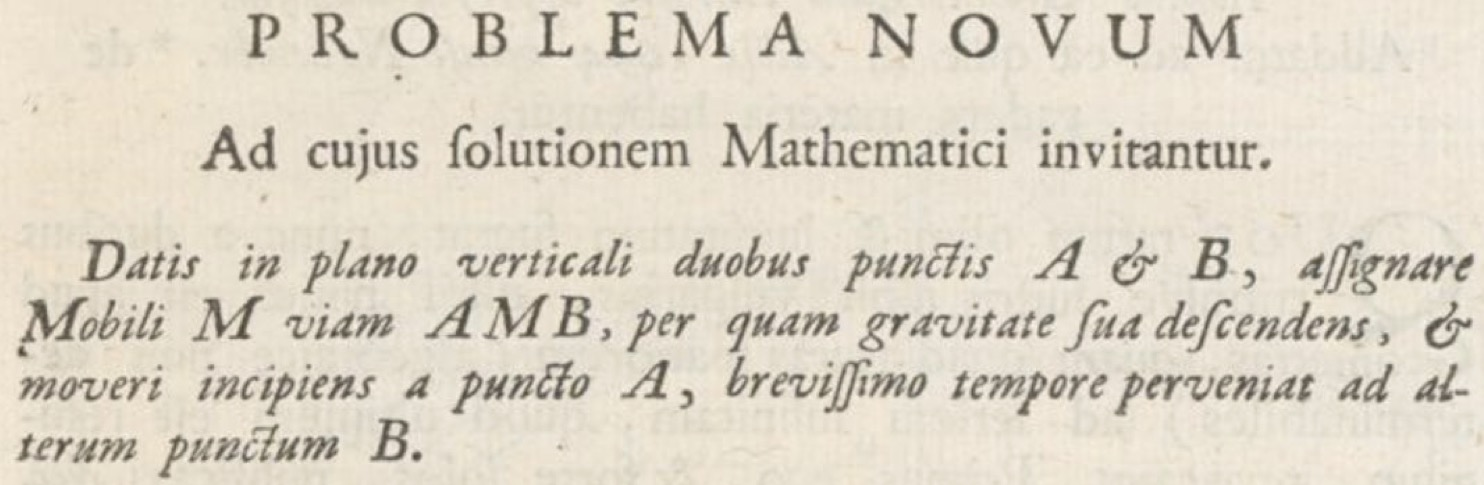
\includegraphics[width=0.8\textwidth]{chapters/020-variation/images/latein.jpg}
\end{center}
Zu deutsch:
\begin{quote}
Neue Aufgabe, zu deren Lösung die Mathematiker eingeladen werden.
Gegeben zwei Punkte $A$ und $B$ in einer vertikalen Ebene, finde
die Bahn $AMB$ eines Punktes $M$, der unter der Wirkung seines
Gewichtes in kürzester Zeit vom Punkt $A$ zum anderen Punkt $B$ absteigt.
\end{quote}
Die Situation der Aufgabenstellung ist in
Abbildung~\ref{buch:variation:fig:brachistochronenproblem}
dargestellt.
Bernoulli hat als Lösung gefunden, dass die Kurve eine Ausschnitt
aus einer Zykloide (in der Abbildung grau) sein muss.
Seine Lösung beruhte auf der Beobachtung, dass sich das Problem analog
zu einem Lichtausbreitungsproblem ist, für welches Fermat bereits
eine Lösung gefunden hat.

Da die Reibung vernachlässigt wird, ist die Energie des Massepunktes
erhalten.
Sie setzt sich aus der potenziellen und der kinetischen Energie
zusammen.
Die potenzielle Energie ist $-mgy$, die kinetische Energie ist
$\frac12mv^2$.
Die Energieerhaltung wird daher zu
\[
E=\frac12mv^2-mgy
\qquad\Rightarrow\qquad
v
=
\sqrt{2g}\!\sqrt{\frac{E}{gm}+y}
=
\!\sqrt{2(C+y)}.
\]
Durch Wahl einer anderen Zeiteinheit kann die Gleichung noch weiter
vereinfacht zu
\(
v = \sqrt{C+y}
\)
vereinfacht werden.
Gesucht ist also die zeitlich kürzeste Bahn eines Teilchens, 
dessen Geschwindigkeit auf bekannte Art $v(y)$ von der vertikalen
Koordinate abhängt.

%
% Das Fermat-Problem
%
\subsection{Das Fermat-Prinzip}
Bereits Fermat hat erkannt, dass das Brechnungsgesetz von Snellius
als Lösung eines Extremalproblems verstanden werden kann.

\begin{satz}[Fermat]
Sie $c/n_i$ die Geschwindigkeit, mit der sich Licht im Medium $M_i$
ausbreitet.
Ein Lichtstrahl von $A_1$ nach $A_2$ geht durch denjenigen Punkt $B$ 
auf der Grenzfläche zwischen den Medien, für den sich die Sinus der
Winkel $\alpha_i$ zwischen den Strahlen und der Normalen zur Grenzfläche
umgekehrt wie die $n_i$ verhalten, wenn also das Brechungsgesetz
\[
\frac{\sin\alpha_1}{\sin\alpha_2}
=
\frac{n_2}{n_1}
\]
gilt.
\end{satz}

\begin{proof}
Ohne der Beschränkung der Allgmeinheit können wir auf die Betrachtung
einer Ebene beschränken, die die beiden Punkte $A_i$ enthält und senkrecht
auf der Grenzfläche steht.
Wir dürfen weiter annehmen, dass die $x$-Achse in der Grenzfläche liegt 
und die Punkte $A_i$ die Koordinaten $(x_i,y_i)$ und der Punkt $B$ die
Koordinaten $(x,0)$ hat.
Es ist derjenige Punkt $x$ zu bestimmen, für den die Lichtzeit entlang 
des Pfades $A_1BA_2$ minimal wird.
Diese Zeit ist
\begin{align*}
t
&=
\frac{\overline{A_1B}}{c/n_1}
+
\frac{\overline{BA_2}}{c/n_2}
\\
ct
&=
n_1\overline{A_1B}
+
n_2\overline{A_2B}
\\
&=
n_1\!\sqrt{(x-x_1)^2 + y_1^2}
+
n_2\!\sqrt{(x_2-x)^2 + y_2^2}
\end{align*}
Das Minimum wird bei einer Nullstelle der Ableitung nach $x$ gefunden,
also bei einer Lösung der Gleichung
\begin{align*}
0
&=
n_1\frac{2(x_1-x)x}{\sqrt{(x_1-x)^2+y_1^2}}
+
n_2\frac{-2(x-x_2)x}{\sqrt{(x_2-x)^2+y_2^2}}.
\intertext{Indem man den zweiten Term auf der rechten Seite auf die linke
Seite bringt und durch $x$ dividiert, erhält man}
n_1
\frac{x_1-x}{\sqrt{(x_1-x)^2+y_1^2}}
&=
n_2
\frac{x-x_2}{\sqrt{(x_2-x)^2+y_2^2}}.
\end{align*}
Der Nenner ist auf beiden Seiten die Hypothenuse eines rechtwinkligen
Dreiecks, welches als Ankathete die Normale zur Grenzfläche hat.
Der Zähler ist die Gegenkathete des Winkels $\alpha_i$ zwischen der
Hypothenuse und der Normalen.
Daher ist der Quotient der Sinus des Winkels oder
\begin{equation}
n_1 \sin\alpha_1 = n_2 \sin\alpha_2.
\label{buch:variation:problem:eqn:snelliusinvariante}
\end{equation}
Die Gleichung~\eqref{buch:variation:problem:eqn:snelliusinvariante}
ist gleichbedeutend mit dem Brechungsgesetz
\[
\frac{\sin\alpha_1}{\sin\alpha_2}
=
\frac{n_2}{n_1}
\]
von Snellius.
\end{proof}

Der Satz von Fermat etabliert das Brechungsgsetz also Lösung eines
Extremalproblems.
Die Natur wählt für einen Lichtstrahl den zeitlich kürzesten Weg.
Der Beweis des Satzes von Fermat zeigt, dass entlang des Lichtstrahls
an jeder Grenzfläche zwischen Medien die Bedingung
\eqref{buch:variation:problem:eqn:snelliusinvariante}
erfüllt.
Wenn die optische Dichte $n$ eine Funktion von $n(y)$ ist, dann
wird der Lichtstrahl nicht nur in diskreten Punkten geknickt, sondern
entlang des ganzen Strahles gekrümmt.
Folgt der Strahl der Kurve $x(y)$, die mit der vertikalen den Winkel
$x'(y) = \tan\alpha(y)$ einschliesst.
Damit lässt sich auch die Sinus-Funktion ausdrücken, es gilt
\[
\sin\alpha(y)
=
\frac{x'(y)}{\pm\!\sqrt{x'(y)^2+1}}.
\]
Aus der Form~\eqref{buch:variation:problem:eqn:snelliusinvariante}
des Brechungsgesetztes wird dann die Gleichung
\begin{equation}
n_1\sin\alpha(y)
=
\frac{n_1(y)x'(y)}{\pm\!\sqrt{x'(y)^2+1}}
=
\operatorname{const}
\qquad\Rightarrow\qquad
\frac{n_1(y)^2x'(y)^2}{x'(y)^2+1}=C.
\label{buch:variation:eqn:fermatdgl}
\end{equation}
Dies ist eine Differentialgleichung für die Funktion $x(y)$.
Sie kann auch in die Form
\[
x'(y)^2
=
\frac{C}{(n_1(y)^2-C)}
\]
gebracht werden.

%
% Das Brachistochronenproblem als Lichtausbreitungsproblem
%
\subsubsection{Das Brachistochronenproblem als Lichtausbreitungsproblem}
Das Fermat-Prinzip besagt, dass ein Lichtstrahl, der sich in einem Medium
mit der Geschwindigkeit $c/n(y)$ ausbreitet, die Gleichung 
\eqref{buch:variation:eqn:fermatdgl} erfüllt.
Beim Brachistochronenproblem ist die Geschwindigkeit $v(y)=\!\sqrt{C-y}$ und 
damit $n(y) = c/\!\sqrt{C-y}$.
Eine Brachistochrone ist also eine Kurve, die die aus
\eqref{buch:variation:eqn:fermatdgl} folgende Gleichung
\begin{equation}
\frac{x'(y)^2}{(1+x'(y)^2)(C-y)} = K
\label{buch:variation:problem:eqn:bernoullidgl}
\end{equation}
erfüllen.

%
% Die Bernoullische Lösung
%
\subsubsection{Die Bernoullische Lösung}
Bernoulli hat gefunden, dass die Brachistochrone ein Zykloidenbogen ist.
Dies lässt sich dadurch verifizieren, dass man die Parametrisierung
einer Zykloide in die
Gleichung~\eqref{buch:variation:problem:eqn:bernoullidgl}
einsetzt.
Die Zykloide hat die Parametrisierung
\[
\left.
\begin{aligned}
x &= r(\varphi - \sin\varphi) 
\\
y &= r(1-\cos\varphi)
\end{aligned}
\right\}
\quad
\text{mit der Ableitung}
\quad
\left\{
\begin{aligned}
\dot{x}(\varphi) &= r(1-\cos\varphi)\\
\dot{y}(\varphi) &= r\sin\varphi
\end{aligned}
\right.
\]
für $\varphi\in\mathbb{R}$.
Die Ableitung ist
\[
x'(y)
=
\frac{\dot{x}(\varphi)}{\dot{y}(\varphi)}
=
\frac{1-\cos\varphi}{\sin\varphi}.
\]
Eingesetzt in \eqref{buch:variation:problem:eqn:bernoullidgl}
wird daraus
\[
\frac{\dot{x}(\varphi)^2}{
(\dot{y}(\varphi)^2 +\dot{x}(\varphi)^2)
(C-r(1-\cos\varphi))
}
=
\frac{(1-\cos\varphi)^2}{
((1-\cos\varphi)^2+\sin^2\varphi)
(C-r+r\cos\varphi)
}
=
K.
\]
Ausmultiplizieren im Nenner ergibt
\[
\frac{(1-\cos\varphi)^2}{
(1-2\cos\varphi+\cos^2\varphi+\sin^2\varphi)
(C-r+r\cos\varphi)
}
=
\frac{1-\cos\varphi}{
2(C-r+r\cos\varphi)
}
\]

%
% Das Brachistochronenproblem als Variationsproblem
%
\subsection{Das Brachistochronenproblem als Variationsproblem
\label{buch:variation:problem:subsection:variationsproblem}}
Die Bernoullische Lösung des Brachistochronenproblems verwendet die
Analogie zum Fermat-Prinzip.
Eine solche Analogie ist nur selten möglich, daher soll das Problem
jetzt in eine Form gebracht werden, in die auch viele ähnliche
Optimierungsproblem gebracht werden können.

Wir erinnern daran, dass die Geschwindigkeit des Massepunktes durch
$v(y)=\sqrt{C-y}$ gegeben ist.
Damit lässt sich die Zeit berechnen, die der Massepunkt entlang der
Lösungskurve braucht, wenn man diese als Funktion $y(x)$ mit beschreibt.
Die Punkte $A$ und $B$ sollen die $x$-Koordinaten $a$ bzw.~$b$ haben.
Für das Kurvenstück zwischen den $x$-Koordinaten $x$ und $x+\Delta x$
braucht der Massepunkt die Zeit
\[
\frac{ \sqrt{\Delta x^2 + \Delta y^2} }{v(y)}
=
\frac{ \sqrt{1 + y'(x)^2} }{ v(y) } \Delta x.
\]
Die Zeit ist das Integral
\begin{equation}
t
=
\int_a^b \frac{\sqrt{1+y'(x)^2}}{v(y(x))}\,dx
=
\int_a^b \sqrt{\frac{1+y'(x)^2}{C-y(x)}}\,dx.
\label{buch:variation:problem:eqn:brachint}
\end{equation}
Der Integrand auf der rechten Seite hängt nur von den Funktion $y(x)$
und $y'(x)$ ab.
Dies kommt vor allem daher, dass die Geschwindigkeit nur von $y$ abhängt,
nicht auch noch von $x$.
Im Allgemeinen wird man also davon ausgehen müssen, dass der Integrand
auch noch von $x$ abhängt.
Die Variationsrechnung befasst sich mit Problemen, in denen Funktionen
gefunden werden müssen, die ein Integral wie das in
\eqref{buch:variation:problem:eqn:brachint}
minimiert oder maximiert werden müssen.

\begin{definition}[Lagrange-Funktion des Brachistochronenproblems]
Die Lagrange-Funk\-tion des Brachistochronenproblems ist der
Integrand des Integrals
\eqref{buch:variation:problem:eqn:brachint},
\index{Lagrange-Funktion}%
also die Funktion
\[
L(x,y,y')
=
\sqrt{\frac{1+y^{\prime 2}}{C-y}}.
\]
\end{definition}

%
% Funktionale
%
\subsection{Funktionale
\label{buch:variation:problem:subsection:funktionale}}
Die Variationsrechnung löst Optimierungsproblem, die von einer
Funktion abhängen.
Um dies mathematisch präzis zu fassen, ist zunächst nötig, die Menge
der in Frage kommenden Funktionen so einzuschränken, dass die interessierende
Grösse überhaupt wohldefiniert ist.

%
% Vektorräume
%
\subsubsection{Vektorräume}
Zunächst sind die gemeinsamen algebraischen Eigenschaften zu charakterisieren,
die wir von den für unsere Untersuchungen zweckmässigen Funktionenmengen
erwarten.

\begin{definition}[Vektorraum]
Ein Vektorraum über den reellen Zahlen $\mathbb{R}$ ist einem Menge $V$ mit
zwei Operationen, der Addition und der Multiplikation mit Skalaren
\begin{align*}
    +\colon V\times V         &\to V : (u,v)\mapsto u+v
&
\cdot\colon \mathbb{R}\times V&\to V : (\lambda,v) \mapsto\lambda v
\end{align*}
mit den folgenden Eigenschaften.
\begin{enumerate}
\item
Es gelten die Assoziativgesetze
\begin{align*}
(u+v)+w&=u+(v+w)&&\text{für alle $u,v,w\in V$}\\
(\lambda \mu)v&=\lambda(\mu v)&&\text{für alle $\lambda,\mu\in\mathbb{R},\;v\in V$.}
\end{align*}
\item
Es gibt einen Vektor $0\in V$ mit der Eigenschaft $0+v=v$ für alle
Vektoren $v\in V$.
\item
Zu jedem Vektor $v\in V$ gibt es den entgegengesetzten Vektor $-v\in V$
mit der Eigenschaft, dass $-v+v=0$ ist.
\item
Die Addition von Vektoren ist kommutativ: $u+v=v+u$ für alle $u,v\in V$.
\item
Es gelten die Distributivgesetze 
\begin{align*}
(\lambda + \mu) v &= \lambda v + \mu v
	&\quad\text{für alle $\lambda,\mu\in\mathbb{R},\;v\in V$}\\
\lambda(u+v)      &= \lambda u + \lambda v
	&\quad\text{für alle $\lambda\in\mathbb{R},\;u,v\in V$}
\end{align*}
\end{enumerate}
\end{definition}

Die Mengen $\mathbb{R}^n$ erfüllen die genannten Eigenschaften, sind
also Vektorräume.
Die Definition eines Vektorraums ist aber viel allgemeiner, insbesondere
gehören dazu auch Mengen von Funktionen.
Damit wird es möglich, die Berechnungen in $\mathbb{R}^n$ auf Funktionen
auszudehnen.
Zum Beispiel bilden die stetigen Funktionen auf einem Intervall einen
Vektorraum, wie das folgende Beispiel zeigt.

\begin{beispiel}
Die Menge
\[
C([a,b])
=
\{f\colon[a,b]\to\mathbb{R}\mid \text{$f$ ist stetig}\}
\]
der stetigen Funktionen bildet einen Vektorraum.
Die Operationen sind die punktweise Addition von Funktionen und die
Multiplikation der Werte mit Skalaren, für $f,g\in C([a,b])$ und
$\lambda\in \mathbb{R}$ ist
\begin{align*}
(f+g)(x) &= f(x)+g(x)
&&\text{und}&
(\lambda f)(x) &= \lambda f(x).
\end{align*}
Entscheidend ist, dass die Addition von Funktionen und die Multiplikation
mit Skalaren nicht aus der Menge herausführt.
Tatsächlich wird in der Analysis gezeigt, dass die Summe stetiger Funktionen
wieder stetig ist und dass die Funktion $x\mapsto \lambda f(x)$ stetig,
wenn $f$ stetig ist.
Die übrigen Eigenschaften sind ebenfalls erfüllt, da sie bereits für die
Funktionswerte erfüllt sind.
\end{beispiel}

%
% Norm und Grenzwerte
%
\subsubsection{Norm und Grenzwerte}
Um Analysis zu betreiben, muss man ausdrücken können, dass eine Folge
von Funktionen konvergiert.
Dazu ist ein Abstandsbegriff zwischen Funktionen nötig.

\begin{definition}[Norm, normierter Raum]
Eine {\em Norm} auf einem Vektorraum $V$ ist eine Abbildung
\index{Norm}%
$\|\cdot\|\colon V\to\mathbb{R}^+_0$ mit nichtnegativen reellen Werten
und den folgenden Eigenschaften
\begin{itemize}
\item Definitheit: $\|v\|\ge 0$ für $v\in V$ mit Gleichheit 
genau dann, wenn $v=0$.
\index{Definitheit}%
\item Absolute Homogenität: Für alle Vektoren $v\in V$ und
\index{Homogenität}%
$\lambda\in\mathbb{R}$ gilt $\|\lambda v\| = |\lambda|\, \|v\|$.
\item Dreiecksungleichung: für alle Vektoren $u,v\in V$ gilt
\index{Dreiecksungleichung}%
$\|u+v\|\le \|u\|+\|v\|$.
\end{itemize}
Ein {\em normierter Raum} ist ein Vektorraum mit einer Norm.
\index{normierter Raum}%
\end{definition}

\begin{beispiel}
Der Vektorraum der stetigen Funktionen kann mit der Supremum-Norm
\[
\|f\| = \sup_{x\in[a,b]} |f(x)|
\]
zu einem normierten Raum gemacht werden.
Die Definitheit ist durch die Definition offensichtlich sichersgtellt.
Für $\|\lambda f\|$ finden wir
\[
\|\lambda f\|
=
\sup_{x\in[a,b]} |\lambda f(x)|
=
|\lambda|\,
\sup_{x\in[a,b]} |f(x)|
=
|\lambda|\, \|f\|,
\]
was die Homogenität zeigt.
Die Dreiecksungleichung folgt aus
\begin{align*}
\|f+g\|
&=
\sup_{x\in[a,b]} |f(x)+g(x)|
\\
&\le
\sup_{x\in[a,b]} (|f(x)|+|g(x)|)
\\
&\le
\sup_{x\in[a,b], y\in[a,b]} (|f(x)|+|g(y)|)
\\
&=
\sup_{x\in[a,b]} |f(x)|
+
\sup_{y\in[a,b]} |g(y)|
=
\|f\| + \|g\|.
\qedhere
\end{align*}
\end{beispiel}

Mit einer Norm ist es jetzt möglich, die Konvergenz von Folgen und den
Begriff des Grenzwertes zu definieren.

\begin{definition}[Cauchy-Folge, Grenzwert]
Eine Folge $(x_n)_{n\in\mathbb{N}}$ in $V$ in einem normierten Raum $V$
mit der Norm $\|\cdot\|$
heisst eine Cauchy-Folge, wenn es für jedes $\varepsilon>0$ eine
\index{Cauchy-Folge}%
$N\in \mathbb{N}$ gibt derart, dass
\[
\| x_n - x_m \| < \varepsilon
\quad\forall n,m\ge N.
\]
Der Vektor $x\in V$ heisst {\em Grenzwert} der Folge $(x_n)_{n\in\mathbb{N}}$,
\index{Grenzwert}%
wenn es zu jedem $\varepsilon > 0$ ein $N\mathbb{N}$ gibt derart, dass
\[
\|x_n-x\| < \varepsilon 
\quad\forall n\ge N.
\]
Die Folge $(x_n)_{n\in\mathbb{N}}$  in $V$ heisst {\em konvergent}, wenn
\index{konvergent}%
$x$ der Grenzwert von $(x_n)_{n\in\mathbb{N}}$ ist.
\end{definition}

Der durch die Supremum-Norm definierte Konvergenzbegriff ist die gleichmässige
Konvergenz.
Zur Erinnerung:
Eine Folge $f_n$ von Funktionen heisst gleichmässig konvergent gegen die
Funktion $f$, wenn es zu jedem
$\varepsilon >0$ ein $N\in\mathbb{N}$ gibt derart, dass
\[
|f_n(x) - f(x)|<\varepsilon\quad\forall n>N\text{ und }x\in [a,b].
\]
Die Supremum-Norm ist
\[
\|f_n(x) - f(x)\|
=
\sup_{x\in[a,b]} |f_n(x)-f(x)| < \varepsilon
\]
für alle $n>N$.
Dies ist genau die Konvergenz in der Norm $\|\cdot\|$.
Aus der Analysis ist bekannt, dass eine gleichmässig konvergente 
Funktionenfolge gegen eine stetige Funktion konvergiert.

\begin{definition}[Banach-Raum]
Ein normierter Raum $V$ heisst ein {\em Banach-Raum},
\index{Banach-Raum}%
wenn jede Cauchy-Folge in $V$ einen Grenzwert hat.
\end{definition}

\begin{beispiel}
Die Menge $C^1([0,2])$
der stetigen Funktionen auf dem Intervall $[0,2]$ ist ein normierter
Raum mit der Norm
\[
\|f\|_1
=
\int_0^2 |f(x)|\,dx,
\]
die auch die $L^1$-Norm heisst.
\index{L1-Norm@$L^1$-Norm}%
Zunächst ist nachzuprüfen, dass dies tatsächlich eine Norm ist.
Die Definitheit und die Homogenität von $\|\cdot\|_1$ ist klar, nur
die Dreiecksungleichung erfordert etwas Arbeit.
Für Funktionen $f,g\in L^1([0,2])$ gilt
\begin{align*}
\|f+g\|_1
&=
\int_0^2 |f(x)+g(x)|\,dx
\\
&\le 
\int_0^2 |f(x)|+|g(x)|\,dx
=
\int_0^2 |f(x)|\,dx
+
\int_0^2 |g(x)|\,dx
=
\|f\|_1+\|g\|_1,
\end{align*}
was die Dreeicksungleichung beweist.

Eine Cauchy-Folge in der $L^1$-Norm muss aber nicht unbedingt einen
stetigen Grenzwert haben.
Die Funktionen
\(
f_n(x) =
\begin{cases}
x^n&\quad x< 1\\
1&\quad x\ge 1
\end{cases}
\)
haben die $L^1$-Norm
\begin{align*}
\|f_n-f_m\|_1
=
\int_0^2 |f_n(x)-f_m|\,dx
\\
&=
\biggl|\int_0^1 x^n-x^m\,dx\biggr|
=
\biggl[
\biggl|
\frac{1}{n+1}x^{n+1}
-
\frac{1}{m+1}x^{m+1}
\biggr|
\biggr]_0^1
\\
&=
\biggl|
\frac{1}{n+1}
-
\frac{1}{m+1}\biggr|.
\end{align*}
Wegen
\[
\|f_n-f_m\|_1
<\varepsilon
\]
für $n,m>2/\varepsilon$ ist $f_n$ eine Cauchy-Folge in $L^1$.
In $L^1$ konvergiert die Folge $f_n$ gegen die Funktion
\[
f(x)
=
\begin{cases}
0&\quad x< 1\\
1&\quad x\ge 1.
\end{cases}
\]
Diese Funktion ist aber nicht stetig, da sie bei $x=1$ einen
Sprung hat.
Bezüglich der $L^1$-Norm ist $C^1([a,b])$ als im Allgemeinen
kein Banach-Raum.
\end{beispiel}

%
% Stetige und differenzierbare Funktionen
%
\subsubsection{Stetige und differenzierbare Funktionen}
Mit der Norm lässt sich auch die Stetigkeit von Abbildungen zwischen
normierten Räumen definieren.

\begin{definition}[Stetigkeit]
Eine Funktion $f\colon U\to V$ zwischen normierten Räumen heisst
{\em stetig im Punkt} $x\in U$, wenn es zu jedem $\varepsilon > 0$
\index{stetig in einem Punkt}%
ein $\delta > 0$
gibt derart, dass
\(
\|f(x)-f(y)\| < \delta
\)
wenn
\(
\|x-y\|<\varepsilon
\).
Eine Funktion $f\colon U\to V$ heisst {\em stetig}, wenn sie in
jedem Punkt von $U$ stetig ist.
\end{definition}

Das Bild einer Folge $x_n\in U$, die gegen $x_0\in U$ konvergiert,
ist eine Folge $f(x_n)$ in $V$.
Man sagt, $y\in V$ sei der Grenzwert von $f(x)$ für $x\to x_0$,
wenn $f(x_n)$ für jede solche Folge $x_n$ gegen $y$ konvergiert.
Der Grenzwert wird auch
\[
\lim_{x\to x_0} f(x)
=
y
\]
geschrieben.
Stetige Funktionen zeichnen sich wie in der Analysis der Funktionen
einer Variablen dadurch aus, dass der Grenzwert der Werte der Funktion
auf einer konvergenten Folge mit dem Funktionswert des Grenzwertes
übereinstimmt.

\begin{satz}
Eine Funktion $f\colon U\to V$ ist genau dann stetig im Punkt $x\in U$,
wenn für jede Folge $x_n$ in $U$ mit Grenzwert $x$ die Folge $f(x_n)$
konvergent ist und
\[
\lim_{n\to\infty} f(x_n) = f(x).
\]
Eine lineare Funktion $f\colon U\to V$ ist genau dann stetig,
wenn für jede Nullfolge $x_n$ in $U$ 
\[
\lim_{n\to \infty} f(x_n) = 0
\]
gilt.
\end{satz}

\begin{definition}
Eine Funktion $f\colon U\to V$ zwischen normierten Räumen heisst
differenzierbar im Punkt $x\in U$ wenn es eine lineare Funktion
$Df(x_0)\colon U\to V$ gibt derart, dass
\[
f(x+v) =f(x) + Df(x_0)\cdot v + o(v),
\]
wobei $o(v)$ bedeutet, dass für diese Funktion
\[
\frac{o(v)}{|v|}\to 0
\quad\text{für $v\to 0$}
\]
gilt.
\end{definition}

Funktionen auf einem Vektorraum mit reellen Werten weren auch
{\em Funktionale} genannt.
\index{Funktional}
Vor dem 20.~Jahrhundert wurde häufig ein Untersschied zwischen
Funktionen von endlich vielen reellen Variablen und Funktionen
von einem unendlichdimensionalen Vektorraum gemacht.
Die Entwicklungen dieses  Abschnittes haben gezeigt, dass eine
solche Unterscheidung nicht gerechtfertigt ist.
Es ist lediglich notwendig, die Definitionen allgemein genug zu
fassen und sich jederzeit über die Funktionenmenge und die zu
verwendende Norm Rechenschaft abzulegen.


%
% 2-fundamtenallemma.tex
%
% (c) 2023 Prof Dr Andreas Müller
%
\section{Das Fundamentallemma
\label{buch:variation:section:fundamentallemma}}
\kopfrechts{Das Fundamentallemma}
Im Fall des endlichdimensionalen Extremalproblems ist aus der
Forderung, dass alle Richtungsableitung verschwinden müssen, 
die Bedingung geworden, dass
\[
v\cdot\grad f = 0
\]
sein muss für alle Vektoren $v\in\mathbb{R}^n$.
Wir haben daraus geschlossen, dass der Gradient $\grad f=0$
sein muss.
Wir hatten dies das endlichdimensionale Fundamentallemma genannt,
wegen $e_k\cdot \grad f = D_kf$ war es eine ziemliche Selbstverständlichkeit.
Bei der Lösung von Variationsproblemen, wo es nicht um endlichdimensionale
Vektoren und das Skalarprodukt, sondern um Funktionen und Integrale
geht, brauchen wir eine ähnliche Aussage für Funktionen.

%
% Positive glatte Funktionen mit kompaktem Träger
%
\subsection{Positive glatte Funktionen mit kompaktem Träger}
Die Aussage des Fundamentallemmas für endlichdimensionale Vektoren 
folgte sofort aus der Tatsache, dass es für jedes $k$ einen Vektor
$e_k$ gibt, der nur in der Koordinaten $k$ von $0$ verschieden ist.
Natürlich gibt es auch Funktionen, die nur in genau einem Punkt
von $0$ verschieden sind.
Eine solche Funktion ist aber im allgemeinen nicht differenzier-
oder integrierbar.
In diesem Abschnitt soll daher gezeigt werden, dass es unendlich
oft stetig differnzierbare Funktionen gibt, die nur in einem beliebig
kleinen vorgegebenen Intervall $\ge 0$ sind.

\begin{definition}[Träger]
Der {\em Träger} einer Funktion $f\colon X\to\mathbb{R}$ ist die Menge
\index{Träger}%
\[
\supp f = \{ x\in X\mid f(x)\ne \}.
\]
\end{definition}

Gesucht ist also eine beliebig oft stetig differenzierbare Funktion,
deren Träger in einem vorgegebenen Intervall $[a,b]$ enthalten ist.
Wir konstruieren so eine Funktion in zwei Schritten.

\input{chapters/020-variation/fig/f.tex}

\begin{satz}
\label{buch:variation:fundamentallemma:satz:glatt}
Die Funktion
\[
f(x)
=
\begin{cases}
e^{-1/x}&\qquad x>0\\
0&\qquad x\le 0
\end{cases}
\]
(siehe auch Abbildung~\ref{buch:variation:fundamentallemma:fig:glatt})
ist beliebig oft stetig differenzierbar.
\end{satz}

\begin{proof}
Es ist klar, dass die Funktion $f$ beliebig oft stetig differenzierbar
ist in jedem Punkt $x\ne 0$.
Es ist also nur nachzuweisen, dass $f(x)$ im Punkt $0$ beliebig
oft stetig differenzierbar ist.

Die ersten drei Ableitungen von $f(x)$ sind
\begin{align}
f'(x) &= \frac{1}{x^2} f(x)
\label{buch:variation:fundamentallemma:eqn:f1}
\\
f''(x) &= \frac{1-2x}{x^4}f(x)
\notag
\\
f'''(x) &= \frac{6x^2-6x+1}{x^6}f(x).
\notag
\end{align}
Daraus lässt sich die Vermutung ableiten, dass
\begin{equation}
f^{(n)}(x)
=
\frac{p_{n-1}(x)}{x^{2n}} f(x)
\label{buch:variation:fundamentallemma:eqn:fabl}
\end{equation}
ist, wobei $p_k(x)$ ein Polynom vom Grad $k$ ist.
Wir beweisen diese Vermutung mit Hilfe von vollständiger Induktion.
Die Induktionsverankerung für die $0$-te Ableitung ist trivial.

Wir nehmen jetzt im Sinne der Induktionsannahme an, dass die $n$-te
Ableitung die Form \eqref{buch:variation:fundamentallemma:eqn:fabl}
hat.
Wir müssen zeigen, dass dann auch $f^{(n+1)}(x)$ diese Form hat.
Dazu berechnen wir
\begin{align}
f^{(n+1)}(x)
&=
\frac{d}{dx}
\frac{p_n(x)}{x^{2n}} f(x)
\notag
\\
&=
\frac{p_n'(x)}{x^{2n}} f(x)
-2n
\frac{p_n(x)}{x^{2n+1}} f(x)
+
\frac{p_n(x)}{x^{2n}} f'(x).
\notag
\intertext{Mit der ersten Ableitung
\eqref{buch:variation:fundamentallemma:eqn:f1} wird dies zu}
&=
\frac{p_n'(x)}{x^{2n}} f(x)
-2n
\frac{p_n(x)}{x^{2n+1}} f(x)
+
\frac{p_n(x)}{x^{2n}} \frac{1}{x^2}f(x)
\notag
\\
&=
\frac{x^2p_n'(x) -2nxp_n(x)+p_n(x)}{x^{2n+2}} f(x).
\label{buch:variation:fundamentallemma:eqn:induktionsschritt}
\end{align}
Die Ableitung $p_n'(x)$ ist ein Polynom vom Grad $n-1$ und damit
ist $x^2p_n'(x)$ ein Polynom vom Grad $n+1$.
Ebenso ist $xp_n(x)$ ein Polynom vom Grad $n+1$ während
$p_n(x)$ ein Polynom vom Grad $n$ ist.
Der Zähler von
\eqref{buch:variation:fundamentallemma:eqn:induktionsschritt}
ist
\[
p_{n+1}(x)
=
x^2p_n'(x)+(1 -2nx)p_n(x),
\]
ein Polynom vom Grad $n+1$.
Damit ist der Induktionsschritt erfolgreich und die Behauptung betreffend
die Form von $f^{(n)}(x)$ ist bewiesen.

Es ist jetzt nur noch zu zeigen, dass der Grenzwert von $f^{(n)}(x)$
für $x\to 0+$ verschwindet.
Da das Polynom $p_n(x)$ stetig ist, folgt
\[
\lim_{x\to 0}
f^{(n)}(x)
=
\lim_{x\to 0}\frac{p_n(x)}{x^{2n}}f(x)
=
p_n(0) \lim_{t\to\infty} t^{2n} e^{-t}
=
0.
\]
Damit ist die beliebige stetige Differenzierbarkeit an der Stelle
$x=0$ gezeigt.
\end{proof}

Die Funktion $f(x)$ von 
Satz~\ref{buch:variation:fundamentallemma:satz:glatt} 
erfüllt noch nicht die Forderung, dass sie nur in einem vorgegebenen
Intervall von $0$ verschieden ist.

\input{chapters/020-variation/fig/g.tex}

\begin{satz}
\label{buch:variation:fundamentallemma:satz:gab}
Sei $f(x)$ die Funktion von
Satz~\ref{buch:variation:fundamentallemma:satz:glatt}.
Dann ist
\[
g_{a,b}(x)
=
f(x-a) f(b-x)
\]
eine unendlich oft stetig differenzierbare, nichtnegative Funktion mit Träger
$\supp g_{a,b}=(a,b)$.
\end{satz}

Die Funktionen $g_{a,b}(x)$ sind beliebig oft differenzierbar und nur im
Intervall $[a,b]$ von $0$ verschieden und sogar positiv.
Weil sie stetig sind, sind sie auch integrierbar, man kann also das
Integral über $\mathbb{R}$ berechnen und die Funktion damit normieren.
Die neue Funktion
\[
\frac{1}{N}
\tilde{g}_{a,b}(x)
\qquad\text{mit}\;
N
=
\int_{-\infty}^{\infty}g_{a,b}(x)\,dx
=
\int_a^b g_{a,b}(x)\,dx
\]
ist immer noch beliebig oft stetig differenzierbar und hat zusätzlich die
Eigenschaft
\[
\int_{-\infty}^{\infty}
\tilde{g}_{a,b}(x)\,dx
=
\int_a^b
\tilde{g}_{a,b}(x)\,dx
=
1.
\]
Wir formulieren dieses Resultat als Satz.

\begin{satz}
\label{buch:variation:satz:gabeins}
Zu jedem Intervall $[a,b]$ gibt es eine beliebig oft stetig
differenzierbare Funktion $g(x)$, genau das Intervall $[a,b]$
als Träger hat und deren Integral über $[a,b]$ den Wert $1$ hat.
\end{satz}

%
% Das Fundamentallemma
%
\subsection{Das Fundamentallemma}
Mit der Funktion $g_{a,b}(x)$ von
Satz~\ref{buch:variation:fundamentallemma:satz:gab}
lässt sich jetzt das Fundamentallemma in der folgenden Form
leicht beweisen.

\begin{satz}[Fundamentallemma]
\label{buch:variation:fundamentallemma:satz:fundamentallemma}
Wenn für die stetige Funktion $f\colon[a,b]\to\mathbb{R}$ 
\begin{equation}
\int_a^b f(x)\varphi(x)\,dx = 0
\label{buch:variation:fundamentallemma:eqn:fundamentalbed}
\end{equation}
gilt für jede beliebig oft stetig differenzierbare Funktion $\varphi(x)$ 
dann ist $f(x)=0$.
Das Resultat gilt selbst dann, wenn
\eqref{buch:variation:fundamentallemma:eqn:fundamentalbed}
nur für beliebig oft stetig differenzierbare Funktionen $\varphi(x)$ 
gilt, die ausserdem an den Intervallenden verschwinden:
$\varphi(a)=\varphi(b)=0$.
\end{satz}

\begin{proof}
Wir zeigen mit Hilfe eines Widerspruchs, dass es keinen Punkt $x_0\in[a,b]$
geben kann, für den $f(x_0)\ne 0$ ist.
Dazu nehmen wir also an, dass $f(x_0)\ne 0$ ist.
Falls $f(x_0)<0$ ist, ersetzen wir $f$ durch $-f$, 
die Bedingung
\eqref{buch:variation:fundamentallemma:eqn:fundamentalbed}
ändert sich dadurch nicht.
\input{chapters/020-variation/fig/fundamentallemma.tex}
Wir dürfen daher annehmen, dass $f(x_0)>0$ ist
(Abbildung~\ref{buch:variation:fundamentallemma:fig:beweis}).
Da $f$ stetig ist, gibt es ein Intervall $[x_0-\varepsilon,x_0+\varepsilon]$
derart, dass $f(x)> \frac12 f(x_0)$ für
$x\in[x_0-\varepsilon,x_0+\varepsilon]$ gilt.
Dann gilt für das Integral
\[
\int_a^b
f(x)
g_{x_0-\varepsilon,x_0+\varepsilon} (x)
\,dx
>
\frac{f(x_0)}{2}
\int_a^b
g_{x_0-\varepsilon,x_0+\varepsilon} (x)
\,dx
>
0
\]
im Widerspruch zur Bedingung
\eqref{buch:variation:fundamentallemma:eqn:fundamentalbed}.
Der Widerspruch zeigt, dass $f(x)=0$ sein muss.
\end{proof}

%
% Skalarproduktformulierung des Fundamentallemmas
%
\subsection{Skalaproduktformulierung des Fundamentallemmas}
Die Richtungsableitung einer Funktion endlich vieler Variablen 
konnte als Skalarprodukt mit dem Gradienten geschrieben werden und
das Fundamentallemma hat besagt, dass der Gradient verschwindet,
wenn alle Richtungsableitungen verschwinden.
Diese Schlussweise ist auch für Funktionen möglich, wenn man Funktionen
ein Skalarprodukt definieren kann.

\begin{definition}[$L^2$-Skalarprodukt]
Das {\em Skalarprodukt} zweier quadratintegrierbarer Funktion $f$ und $g$
auf dem Intervall $[a,b]$ ist definiert durch
\[
\langle f,g\rangle
=
\int_a^b f(x)g(x)\,dx.
\]
\end{definition}

\begin{satz}[Fundamentallemma, Skalarproduktform]
Wenn für eine stetige Funktion $f\colon[a,b]\to\mathbb{R}$ das Skalarprodukt
\[
\langle f,\varphi\rangle = 0
\]
ist für jede unendlich oft differenzierbare Funktion $\varphi$ auf dem
Intervall $[a,b]$, dann ist $f=0$.
\end{satz}



%
% 3-eulerlagrange.tex
%
% (c) 2023 Prof Dr Andreas Müller
%
\section{Die Euler-Lagrange Differentialgleichung
\label{buch:variation:section:eulerlagrange}}
\kopfrechts{Die Euler-Lagrange Differentialgleichung}
Das Neuartige an der Aufgabenstellung des Brachistochronenproblems
war, dass eine Funktion gesucht war, so dass ein damit gebildetes
Integral eine Minimaleigenschaft erfüllt.
Für die damalige Mathematik war die Aufgabe, eine Funktion zu finden,
nicht neu.
Die Theorie der Differentialgleichungen war bereits entwickelt,
Newton hat die Infinitesimalrechnung ja erfunden, um damit die
Bewegungsgleichungen der Physik zu formulieren und zu lösen.
In einer Differentialgleichung werden Werte und Ableitungen einer
Funktion an einer einzigen Stelle miteinander verbunden.
Etwas salop formuliert sagt die Differentialgleichung in jedem
Punkt, in welche Richtung und mit welcher Krümmung die Funktionskurve
weiter zu zeichnen ist.

Im Brachistochronenproblem tragen aber alle Werte der gesuchten
Funktion zum Integral bei, es scheint daher auf den ersten Blick
nicht möglich, das Problem durch schrittweise Konstruktion
``von Punkt zu Punkt'' der Lösungskurve zu konstruieren.

Bernoullis Lösung des Brachistochrononproblems beruht auf der
Beobachtung, dass sich die Bedinung für die schnellste Bahn
durch eine Bedingung ersetzen lässt, die in jedem einzelnen
Punkt ausgewertet werden kann.
Das von ihm verwendete Fermat-Prinzip wurde ursprünglich ebenfalls
als eine globale Eigenschaft eines Lichtstrahls formuliert.
Aus dem Fermat-Prinzip folgt aber das Brechungsgesetz, welches
sagt, dass die Richtung eines Strahls in einem Punkt genau dann
ändert, wenn sich dort auch der Brechungsindex der beiden Medien
ändert.
Das Fermat-Prinzip ist also ein Beispiel dafür, wie eine globale
Bedingung erfüllt werden kann, indem einer lokalen Regel in jedem
Punkt gefolgt wird.

Es ist das Verdienst von Euler und Lagrange, zu erkennen, dass diese
Übersetzung eines globalen Variationsproblems in ein lokales 
Problem immer möglich ist.
Es entsteht dabei die Euler-Lagrange-Differentialgleichung, welche
die Problemstellung auf die Lösung einer Differentialgleichung
reduziert.
Damit ist ein allgemein anwendbares Lösungsverfahren gefunden.
Zu einem Variationsproblem lässt sich immer eine Differentialgleichung
finden, welche die gesuchte Funktion als Lösung hat.

In diesem Abschnitt soll dieser indirekte Weg der Lösung von
Variationsaufgaben dargestellt werden.
Wir werden später zeigen, dass diese Vorgehensweise nicht immer
erfolgreich sein kann.
Zum Beispiel werden wir in Kapitel~\ref{buch:chapter:nichtdiff}
Variationsprobleme kennenlernen, deren Lösungskurven nicht
differenzierbar sind und daher auch nicht von einer Differentialgleichung
gefunden werden können.
Im Kapitel~\ref{buch:chapter:direkt} werden daher die sogenannten
direkten Methodn vorgestellt, die den Umweg über eine
Differentialgleichung vermeiden.

%
% Die Lagrange-Funktion
%
\subsection{Die Lagrange-Funktion
\label{buch:variation:eulerlagrange:subsection:lagrange-funktion}}
Wir betrachten Variationsproblem der folgenden Art.
Gesucht ist eine auf dem Intervall $[x_0,x_1]$ definirte
Funktion $y(x)$, die das Integral
\begin{equation}
I(y)
=
\int_{x_0}^{x_1}
F(x, y(x), y'(x))
\,dx
\label{buch:variation:eulerlagrange:eqn:funktional}
\end{equation}
maximiert oder minimiert.
Der Ausdruck~\eqref{buch:variation:eulerlagrange:eqn:funktional}
wird ein Funktional genannt.
Die Funktion
\[
F
\colon
\mathbb{R}\times
\mathbb{R}\times
\mathbb{R}
\to
\mathbb{R}
\]
von drei Variablen heisst die {\em Lagrange-Funktion}
des Funktionals \eqref{buch:variation:eulerlagrange:eqn:funktional}.

\begin{beispiel}
Die Lagrange-Funktion des Brachistochronenproblems ist
\[
F(x,y,y')
=
\sqrt{ \frac{1+y^{\prime 2}}{y} }.
\]
Die Funktion hängt nicht von $x$ ab, was bedeutet, dass eine
Verschiebung in $x$-Richtung die Form der Lösungsfunktion des
Variationsproblems nicht ändert.
\end{beispiel}

\begin{beispiel}
\label{buch:variation:eulerlagrange:beispiel:gerade}
Wir formulieren die Aufgabe, die kürzeste Verbindung der Punkte
$(x_0,y_0)$ und $(x_1,y_1)$ in einer Ebene zu finden, als Variationsproblem.
Die Länge einer Kurve $y(x)$ ist das Integral
\[
l(y)
=
\int_{x_0}^{x_1}
\sqrt{1+y'(x)^2}\,dx.
\]
Daraus lesen wir ab, dass die Lagrange-Funktion dieses Variationsproblems
\begin{equation}
F(x,y,y') = \sqrt{1+y^{\prime 2}}
\label{buch:variation:eulerlagrange:eqn:geradeL}
\end{equation}
ist.
Die Funktion hängt weder von $x$ noch von $y$ ab.
Dies ist auch zu erwarten, denn die Länge einer Kurve hängt nicht davon
ob, wo in der Ebene sie platziert ist.
Eine Verschiebung in $x$-Richtung würde das $x$-Argument ändern,
eine Verschiebung in $y$-Richtung die $y$-Werte.
Wäre $F$ von $x$ oder $y$ abhängig, könnte auch die Länge der Kurve
davon abhängen.
\end{beispiel}

%
% Euler-Lagrange_Differentialgleichung
%
\subsection{Euler-Lagrange-Differentialgleichung
\label{buch:variation:eulerlagrange:subsection:dgl}}
\input{chapters/020-variation/fig/variation0.tex}
Das Maximum oder Minimum einer Funktionen mehrere Variablen wurde
gefunden, indem die Richtungsableitung berechnet und $=0$ gesetzt
wurde.
Um die Funktion zu bestimmen, die ein Funktional $I(y)$ zu einem
Maximum oder Minimum macht, versuchen wir, die Idee der Richtungsableitung
für ein Funktional nachzuahmen.
Wir nehmen daher an, dass $y(x)$ eine Funktion ist, die das Funktional
$I(y)$ zu einem Minimum macht.
Für die Richtungsableitung addieren wir ein Vielfaches einer
Funktion $\eta(x)$, die Summe $y(x)+\varepsilon\eta(x)$ entspricht
dann einer Geraden mit Richtung $\eta(x)$ im Funktionenraum
(Abbildung~\ref{buch:variation:fig:variation0}).
Die Funktionen $y(x)+\varepsilon\eta(x)$ sind aber nur dann Kandidaten
für eine Lösung des Problems, wenn immer noch
\begin{align*}
y(x_0) + \varepsilon \eta(x_0) &= y_0
&&\text{und}&
y(x_1) + \varepsilon \eta(x_1) &= y_1
\end{align*}
gilt.
Dies ist nur möglich, wenn $\eta(x_0)=\eta(x_1)=0$ ist.

Wir berechnen jetzt die Ableitung der Funktion
$\varepsilon\mapsto I(y+\varepsilon\eta )$ an der Stelle $\varepsilon=0$.
Da die Intervallgrenzen nicht von $\varepsilon$ abhängen, können wir
die Ableitung unter das Integral nehmen:
\begin{align*}
\frac{d}{d\varepsilon}
I(y+\varepsilon\eta)
&=
\int_{x_0}^{x_1}
\frac{d}{d\varepsilon}
F(x,y(x)+\varepsilon\eta(x),y(x)+\varepsilon\eta'(x))
\,dx.
\intertext{Da $F$ differenzierbar ist, kann die Ableitung mit der
Kettenregel berechnet werden, sie ist}
&=
\int_{x_0}^{x_1}
\frac{\partial F}{\partial y}
(x,y(x)+\varepsilon\eta(x),y(x)+\varepsilon\eta'(x))
\eta(x)
\\
&\qquad
+
\frac{\partial F}{\partial y'}
(x,y(x)+\varepsilon\eta(x),y(x)+\varepsilon\eta'(x))
\eta'(x)
\,dx.
\intertext{Uns interessiert aber nur der Wert an der Stelle $\varepsilon=0$,
er ist}
\frac{d}{d\varepsilon}
I(y+\varepsilon\eta)
\bigg|_{\varepsilon=0}
&=
\int_{x_0}^{x_1}
\frac{\partial F}{\partial y}
(x,y(x),y'(x))
\,
\eta(x)
+
\frac{\partial F}{\partial y'}
(x,y(x),y'(x))
\,
\eta'(x)
\,dx
=0.
\end{align*}
Das Integral hängt von den verschiedenen Faktoren $\eta(x)$ und
von $\eta'(x)$ in den beiden Termen unter dem Integral ab.
Wir integrieren den zweiten Term partiell 
\begin{align*}
\int_{x_0}^{x_1}
\frac{\partial F}{\partial y'}(x,y(x),y'(x))\,\eta'(x)\,dx
&=
\biggl[
\frac{\partial F}{\partial y'}(x,y(x),y'(x))\,\eta(x)
\biggr]_{x_0}^{x_1}
\\
&\qquad
-
\int_{x_0}^{x_1}
\frac{d}{dx}
\frac{\partial F}{\partial y'}(x,y(x),y'(x))\,\eta(x)\,dx.
\end{align*}
Da $\eta(x_0)=\eta(x_1)=0$ verschwindet der erste Term
auf der rechten Seite, es bleibt
\[
\frac{d}{d\varepsilon}
I(y+\varepsilon\eta)
\bigg|_{\varepsilon=0}
=
\int_{x_0}^{x_1}
\biggl(
\frac{\partial F}{\partial y}
(x,y(x),y'(x))
-
\frac{d}{dx}
\frac{\partial F}{\partial y'}
(x,y(x),y'(x))
\biggr)
\eta(x)
\,dx.
\]
Dies kann auch als Skalarprodukt
\[
\biggl\langle 
\frac{\partial F}{\partial y}
(x,y(x),y'(x))
-
\frac{d}{dx}
\frac{\partial F}{\partial y'}
(x,y(x),y'(x))
,
\eta(x)
\biggr\rangle
=
0
\]
geschrieben werden.
Da dies für jede differenzierbare Funktion $\eta$ mit Randwerten
$\eta(x_0)=\eta(x_1)$ gelten muss, folgt nach dem
Fundamentallemma~\ref{buch:variation:fundamentallemma:satz:fundamentallemma},
der folgende Satz. 

\begin{satz}[Euler-Lagrange]
\label{buch:variation:eulerlagrange:satz:eulerlagrange}
Wenn die mindestens zweimal stetig differenzierbare Funktion $y(x)$
unter allen solchen Funktionen mit $y(x_0)=y_0$ und $y(x_1)=y_1$
das Funktional
\[
I(y)
=
\int_{x_0}^{x_1}
F(x,y(x),y'(x))\,dx
\]
zu einem Maximum oder Minimum macht, dann ist $y(x)$ eine Lösung der
gewöhnlichen Differentialgleichung
\begin{equation}
\frac{d}{dx}
\frac{\partial F}{\partial y'}(x,y(x),y'(x))
-
\frac{\partial F}{\partial y}(x,y(x),y'(x))
=
0.
\label{buch:variation:eulerlagrange:eqn:eulerlagrange}
\end{equation}
Sie heisst die {\em Euler-Lagrange-Differentialgleichung}.
\end{satz}

Eine Lösung des Variationsproblems kann also als Lösung der
Euler-Lagrange-Dif\-fe\-ren\-tial\-glei\-chung mit den Randwerten
$y(x_0)=x_0$ und $y(x_1)=y_1$ gefunden werden.
Die Bedingung ist notwendig, aber nicht hinreichend.
Wie bei der Bestimmung eines Extremums bei Funktionen endlich
vieler Variablen garantiert das Verschwinden der Richtungsableitung
nicht, dass auch tatsächlich ein Extremum vorliegt.
Man sagt daher auch, dass eine Lösung $y(x)$ der
Euler-Lagrange-Differentialgleichung das Funktional $I(y)$
stationär macht.

Eine weitere Einschränkung ist, dass die Herleitung der
Euler-Lagrange-Differential\-gleichung vorausgesetzt hat,
dass die Lösungsfunktion $y(x)$ mindestens zweimal 
stetig differenzierbar ist.
Es gibt aber durchaus Variationsprobleme, deren Lösungen
nicht differenzierbar sind, dazu mehr im Kapitel~\ref{buch:chapter:nichtdiff}.

\begin{beispiel}
\label{buch:variation:eulerlagrange:beispiel:gerade}
Wir lösen das Variationsproblem von Beispiel
\ref{buch:variation:eulerlagrange:beispiel:gerade}
mit der Lagrange-Funk\-tion
\eqref{buch:variation:eulerlagrange:eqn:geradeL}.
Da die Lagrange-Funktion nicht von $y$ abhängt, bleibt von der 
Euler-Lagrange-Gleichung nur
\[
\frac{d}{dx}
\frac{\partial L}{\partial y'}(x,y(x),y'(x))
=
0
\]
übrig.
Berechnung der Ableitung liefert
\begin{equation}
\frac{\partial}{\partial y'}
\sqrt{1+y^{\prime 2}}
=
\frac{y'}{\sqrt{1+y^{\prime 2}}}.
\label{buch:variation:eulerlagrange:eqn:ableitungFyp}
\end{equation}
Die Ableitung nach $x$ ergibt
\begin{align*}
\frac{d}{dx}
\frac{\partial}{\partial y'}
\sqrt{1+y^{\prime 2}}
&=
\frac{d}{dx}
\frac{y'}{\sqrt{1+y^{\prime 2}}}
\\
&=
\frac{
y''\sqrt{1+y^{\prime 2}}-y'\cdot \frac{y'y''}{\sqrt{1+y^{\prime 2}}}
}{
1+y^{\prime 2}
}
\\
&=
y''
\frac{
1+y^{\prime 2}-y^{\prime 2}
}{
(1+y^{\prime 2})^{\frac32}
}.
\intertext{Die Euler-Lagrange-Differentialgleichung ist daher}
0
&=
\frac{y''}{(1+y^{\prime 2})^{\frac32}} .
\end{align*}
Der Nenner auf der rechten Seite ist immer $\ge 1$, die Gleichung kann
also nur erfüllt sein, wenn $y''=0$ ist.
Die Funktion $y(x)$ muss also eine lineare Funktion $y=ax+b$ sein.
Die Randbedingung wird erfüllt für die Geradengleichung
\[
y(x)
=
\frac{y_1-y_0}{x_1-x_0}(x-x_0) + y_0.
\]
Kürzeste Verbindungen in der Ebene sind daher Geraden.
\end{beispiel}

%
% Freie Randbedingungen
%
\subsection{Freie Randbedingungen
\label{buch:variation:eulerlagrange:subsection:freierb}}
In der Herleitung der Euler-Lagrange-Differentialgleichung wurde angenommen,
dass die Endpunkte der Lösungsfunktion durch $y(x_0)=y_0$ und $y(x_1)=y_1$
fest vorgegeben sind.
Diese Voraussetzung soll in diesem Abschnitt abgeschwächt werden.
Die Funktionswerte in den Endpunkten sollen also nicht mehr fest
vorgegeben sein.

\begin{beispiel}
\label{buch:variation:eulerlagrange:beispiel:freiegerade}
Im Beispiel~\ref{buch:variation:eulerlagrange:beispiel:gerade}
wurde die kürzeste Kurve zwischen zwei Punkten in der Ebene
gesucht und wie erwartet eine Gerade als Lösung gefunden.
Wenn die Werte $y_0$ und $y_1$ jetzt nicht mehr vorgegeben sind,
wird die kürzeste Verbindung zwischen den beiden Geraden
$x=x_0$ und $x=x_1$ gesucht.
Die Lösung dieses Problems ist nicht eindeutig, jede horizontale
Strecke mit $y_0=y_1$ ist eine Lösung.
\end{beispiel}

Das Beispiel zeigt, dass es im Allgemeinen immer noch die Vorgabe
eines der beiden Randwerte braucht, um die Lösung eindeutig zu
bestimmen.
Wir lösen daher die folgende Aufgabe.

\begin{aufgabe}
Gesucht ist eine zweimal stetig differnzierbare Funktion $y(x)$ auf
dem Intervall $[x_0,x_1]$ mit $y(x_0)=y_0$, die das Integral
\[
I(y)
=
\int_{x_0}^{x_1} F(x,y(x),y'(x))\,dx
\]
zu einem Extremum macht.
Am rechten Ende des Intervalls ist der Funktion $y(x)$ keine
Randbedingung auferlegt.
\end{aufgabe}

\begin{proof}[Lösung]
\input{chapters/020-variation/fig/variation1.tex}
Sei $y(x)$ eine Lösung der Aufgabe und sei $y_1:=y(x_1)$ der Wert
der Lösung am rechten Rand des Intervalls.
Wir berechnen wieder die Variation von $I(y)$ mit Hilfe von
stetig differenzierbaren Funktionen $\eta(x)$, die jetzt aber 
nur noch die Bedingungn $\eta(x_0)=0$ erfüllen müssen
(Abbildung~\ref{buch:variation:fig:variation1}).
Die Richtungsableitung ist wie früher
\begin{align*}
\frac{d}{d\varepsilon}
I(y+\varepsilon\eta)
\bigg|_{\varepsilon=0}
&=
\frac{d}{d\varepsilon}
\int_{x_0}^{x_1}
F(x,y(x)+\varepsilon\eta(x),y'(x)+\varepsilon\eta'(x))\,dx
\\
&=
\int_{x_0}^{x_1}
\frac{\partial F}{\partial y}(x,y(x),y'(x)) 
\eta(x)
+
\frac{\partial F}{\partial y'}
(x,y(x),y'(x))
\eta'(x)
\,dx
\intertext{und mit partieller Integration}
&=
\biggl[
\frac{\partial F}{\partial y'}(x,y(x),y'(x)) \eta(x)
\biggr]_{x_0}^{x_1}
\\
&\qquad
+
\int_{x_0}^{x_1}
\biggl(
\frac{\partial F}{\partial y}(x,y(x),y'(x))
-
\frac{d}{dx}
\frac{\partial F}{\partial y'}(x,y(x),y'(x))
\biggr)
\,
\eta(x)
\,dx.
\end{align*}
Im Gegensatz zu früher können wir jetzt aber nicht mehr
schliessen, dass der erste Term verschwindet, da $y(x_1)$ nicht
mehr als $=0$ verausgesetzt wird.
Vielmehr erhalten wir für die erste Variation
\begin{equation*}
\delta I(y)
=
\frac{\partial F}{\partial y'} (x_1,y(x_1),y'(x_1)) \eta(x_1)+
\int_{x_0}^{x_1}
\biggl(
\frac{\partial F}{\partial y}(x,y(x),y'(x))
-
\frac{d}{dx}
\frac{\partial F}{\partial y'}(x,y(x),y'(x))
\biggr)
\,
\eta(x)
\,dx.
\end{equation*}
Die Klammer im Integral ist von der Euler-Lagrange-Differentialgleichung
her bekannt, aber es ist ein weiterer hinzugekommen, der genau dann
verschwindet wenn auch $\eta(x_1)=0$ ist.

Dann ist $y(x)$ natürlich erst recht eine Lösung des Problems, das
Funktional $I(y)$ mit den {\em zwei} Randbedingungen
$y(x_0)=y_0$ und $y(x_1)=y_1$ zu einem Extremum zu machen, also
muss die Funktion $y(x)$ sicher die Euler-Lagrange-Differentialgleichung
erfüllen.
Die Klammer im Integral wird daher verschwinden, die Variation
reduziert sich auf den ersten Term
\[
\delta I(y)
=
\frac{\partial F}{\partial y'} (x_1,y(x_1),y'(x_1)) \eta(x_1)
=
0.
\]
Sie verschwindet nur dann für alle zulässigen Funktionen $\eta(x)$, wenn
\begin{equation*}
\frac{\partial F}{\partial y'}(x_1,y(x_1),y'(x_1))=0
\end{equation*}
gilt.
Dies ist eine zusätzliche Randbedingung für die Funktion $y(x)$, geschrieben
in einer impliziten Form.
\end{proof}

Wir halten das Resultat der Aufgabenlösung als Satz fest:

\begin{satz}
\label{buch:variation:eulerlagrange:satz:zusaetzlicherb}
Wenn die zweimal stetig differenzierbare Funktion $y(x)$ mit dem
Randwert $y(x_0)=y_0$ das Integral
\[
I(y)
=
\int_{x_0}^{x_1} F(x,y(x),y'(x))\,dx
\]
zu einem Extremum macht, dann erfüllt sie am rechten Intervallende
die Randbedingung
\begin{equation}
\frac{\partial F}{\partial y'}(x_1,y(x_1),y'(x_1))=0.
\label{buch:variation:eulerlagrange:eqn:zusaetzlicherb}
\end{equation}
zusätzlich zur Euler-Lagrange-Gleichung für die Lagrange-Funktion $F$.
\end{satz}

\begin{beispiel}
\label{buch:variation:eulerlagrange:beispiel:einseitigegerade}
Wir betrachten wieder das Funktional
\[
I(y)
=
\int_{x_0}^{x_1}
\sqrt{1+y^{\prime 2}(x)}
\,dx
\]
mit der einzigen Randbedingung $y(x_0)=y_0$, der Funktionswert auf 
der rechten Seite ist nicht vorgebeben.
Der Satz~\eqref{buch:variation:eulerlagrange:satz:zusaetzlicherb}
besagt zunächst, dass die Lösungsfunktion wieder eine Gerade sein
muss, da die Euler-Lagrange-Gleichung erfüllt sein muss.
Zusätzlich muss aber auch die Randbedingung
\eqref{buch:variation:eulerlagrange:eqn:zusaetzlicherb}
am rechten Ende des Intervalls erfüllt sein.
Die Ableitung der Lagrange-Funktion ist in diesem Fall durch
\eqref{buch:variation:eulerlagrange:eqn:ableitungFyp}
gegeben, es muss also
\[
\frac{y'(x_1)}{\sqrt{1+y'(x_1)^2}}
=
0
\qquad\Rightarrow\qquad y'(x_1)=0
\]
gelten.
Die Lösung ist daher wie erwartet eine horizontale Strecke.
\end{beispiel}



%
% 5-hoehereableitungen.tex
%
% (c) 2023 Prof Dr Andreas Müller
%
\section{Höhere Ableitungen
\label{buch:variation:section:hoehereableitungen}}
\kopfrechts{Höhere Ableitungen}
Das Beispiel der Spline-Interpolation in
Abschnitt~\ref{buch:nichtdiff:section:splines}
zeigt, dass es manchmal
nötig ist, höhere Ableitungen als die erste in einem Funktional
zu berücksichtigen.
In diesem Abschnitt wird die Theorie der ersten Variation auf
Funktionale erweitert, die von beliebigen Ableitungen der Funktion $y(x)$
abhängen.

%
% Lagrange-Funktion mit höheren Ableitungen
%
\subsection{Lagrange-Funktion mit höheren Ableitungen}
Die Euler-Lagrange-Differentialgleichung wurde bisher für Funktionale
hergeleitet, deren Lagrange-Funktion von $x$, der Funktion $y(x)$ und
der ersten Ableitung $y'(x)$ abhängen.

\begin{definition}
Eine Funktion $L(x,y,y',\dots,y^{(n)})$ heisst eine Lagrange-Funktion
der Ordnung $n$.
\index{Lagrange-Funktion $n$-ter Ordnung}%
\end{definition}

\begin{beispiel}
Das Variationsproblem für die Spline-Integration hat die Lagrange-Funktion
zweiter Ordnung
\[
L(x,y,y',y'') = y^{\prime\prime 2}
\]
verwendet.
\end{beispiel}

Ein elastischer Stab speichert bei Verbiegung Energie, deren Dichte
entlang des Stabes proportional zur Krümmung ist.
Ist $s\mapsto \gamma(s)\in\mathbb{R}^2$ eine differenzierbare
Parametrisierung einer ebenen Kurve, die die Form eines dünnen elastischen
Stabes beschreibt, dann ist die Gesamtenergie des Stabes bis auf
eine Konstante durch das Integral
\[
E
=
\int_a^b \kappa(s)^2 \,ds
\]
gegeben
Ist $s$ ein Bogenlängenparameter, also $|\dot{\gamma}(s)|=1$, dann ist
die Krümmung die zweite Ableitung, also
\[
I = \int_a^b \ddot{\gamma}(s)^2\,ds.
\]
Diese Parameterdarstellung ist aber nicht die Form, in der wir bis jetzt
Kurven in der Ebene beschreiben konnten.

Sei $y(x)$ eine Funktion, deren Graph einen elastisch verbogenen Stab
in der Ebene beschreibt.
Die Krümmung des Graphen kann nach
\[
\kappa(x)
=
\frac{y''(x)}{(1+y'(x)^2)^{\frac32}}
\]
berechnet werden.
Die Energie des Stabes wird dann
\[
E
=
\int_a^b \frac{y''(x)^2}{(1+y'(x)^2)^3}\,dx.
\]
Die Lagrange-Funktion des Problems der Biegung eines Stabes ist daher
\[
L(x,y,y',y'')
=
\frac{y^{\prime\prime 2}}{(1+y^{\prime 2})^3}.
\]

%
% Die verallgemeinerte Euler-Lagrange-Differentialgleichung
%
\subsection{Die verallgemeinerte Euler-Lagrange-Differentialgleichung}
Auch für ein Variationsproblem mit einer Lagrange-Funktion, die höhere
Ableitungen enthält, lässt sich mit der mehr oder weniger gleichen
Vorgehensweise eine Differentialgleichung für die gesuchte Funktion
$y(x)$ herleiten.
Wie auch im Beispiel zur Spline-Interpolation in
Abschnitt~\ref{buch:nichtdiff:section:splines} angedeutet, wird es
notwendig sein, mehrmals partiell zu integrieren.

Sei also $L(x,y,y',\dots,y^{(n)})$ eine Lagrange-Funktion $n$-ter Ordnung
und sei eine Funktion $y(x)$ gesucht, die ein kritischer Punkt des Funktionals
\[
I(y)
=
\int_a^b L\bigl(x,y(x),y'(x),\dots,y^{(n)}(x)\bigr)\,dx
\]
ist.
Wir berechnen wieder die erste Variation mit Hilfe einer beliebig
oft differenzierbaren Funktion $\eta(x)$, welche in den Endpunkten
des Intervalls zusammen mit allen Ableitungen verschwindet.
Die Variation ist definiert als die Richtungsableitung in Richtung
von $\eta(x)$ als
\begin{align*}
\delta I
&=
\frac{d}{dt}
\int_a^b
L\bigl(x,y(x)+t\eta(x),y'(x)+t\eta'(x),\dots,y^{(n)}(x)+t\eta^{(n)}(x)\bigr)
\,dx\biggl|_{t=0}.
\intertext{Durch Ableitung nach $t$ finden wir}
&=
\int_a^b
\frac{\partial L}{\partial y}\bigl(x,y(x),y'(x),\dots,y^{(n)}(x)\bigr)
\,
\eta(x)
+
\frac{\partial L}{\partial y'}\bigl(x,y(x),y'(x),\dots,y^{(n)}(x)\bigr)
\,
\eta'(x)
\\
&\qquad
+
\dots
+
\frac{\partial L}{\partial y^{(n)}}\bigl(x,y(x),y'(x),\dots,y^{(n)}(x)\bigr)
\,
\eta^{(n)}(x)
\,dx.
\end{align*}
Die Terme mit Ableitungen von $\eta(x)$ können durch partielle
Integration in Terme umgewandelt werden, die nur die Funktion 
$\eta(x)$ enthalten:
\begin{align*}
\delta I
&=
\int_a^b
\frac{\partial L}{\partial y^{(k)}}
\bigl(x,y(x),y'(x),\dots,y^{(n)}(x)\bigr)
\,
\eta^{(k)}(x)
\,dx
\\
&=
\biggl[
\frac{\partial L}{\partial y^{(k)}}
\bigl(x,y(x),y'(x),\dots,y^{(n)}(x)\bigr)
\,
\eta^{(k-1)}(x)
\biggr]_a^b
\\
&\qquad
-
\int_a^b
\frac{d}{dx}
\frac{\partial L}{\partial y^{(k)}}
\bigl(x,y(x),y'(x),\dots,y^{(n)}(x)\bigr)
\,
\eta^{(k-1)}(x)
\,dx.
\intertext{Da die Ableitungen von $\eta(x)$ in den Intervallenden
verschwinden, ist dies gleichbedeutend mit}
&=
-\int_a^b \frac{d}{dx} \frac{\partial L}{\partial y^{(k)}}
\bigl(x,y(x),y'(x),\dots,y^{(n)}(x)\bigr)
\,
\eta^{(k-1)}(x)
\,dx.
\intertext{Durch Iterieren dieser Rechnung erhalten wir}
&=
(-1)^{k}
\int_a^b
\frac{d^k}{dx^k}
\frac{\partial L}{\partial y^{(k)}}
\bigl(x,y(x),y'(x),\dots,y^{(n)}(x)\bigr)
\,
\eta(x)
\,dx.
\end{align*}
Die Variation kann jetzt als
\begin{align*}
\delta I
&=
\int_a^b
\biggl(
\frac{\partial L}{\partial y}
-
\frac{d}{dx}
\frac{\partial L}{\partial y'}
+
\frac{d^2}{dx^2}
\frac{\partial L}{\partial y''}
-
\dots
+
(-1)^n
\frac{d^n}{dx^n}
\frac{\partial L}{\partial y^{(n)}}
\biggr)
\,
\eta(x)
\,dx
\end{align*}
geschrieben werden.
Die Variation $\delta I$ muss für jede Wahl von $\eta(x)$ verschwinden,
daher folgt aus dem Fundamentallemma, dass $y(x)$ die Differentialgleichung
\begin{equation}
\frac{\partial L}{\partial y}
-
\frac{d}{dx}
\frac{\partial L}{\partial y'}
+
\frac{d^2}{dx^2}
\frac{\partial L}{\partial y''}
-
\dots
+
(-1)^n
\frac{d^n}{dx^n}
\frac{\partial L}{\partial y^{(n)}}
=
0
\label{buch:variation:hohere:eqn:eulerlagrange}
\end{equation}
erfüllen muss.
Man beachte, dass wir in dieser Rechnung stillschweigend annehmen,
dass die Funktion $y(x)$ genügend oft stetig differenzierbar ist,
so dass die einzelnen Terme der Differentialgleichung
\eqref{buch:variation:hohere:eqn:eulerlagrange} wohldefiniert sind.

\begin{satz}[Euler-Lagrange-Differentialgleichung]
Eine genügend oft differenzierbare Funktion $y(x)$ ist ein stationärer
Punkt des Integrals
\[
I
=
\int_a^b
L\bigl(x,y(x),y'(x),\dots,y^{(n)}(x)\bigr)
\,dx
\]
mit der Lagrange-Funktion $n$-ter Ordnung $L(x,y,y',\dots,y^{(n)})$,
wenn sie die die Euler-Lagrange-Differentialgleichung
\eqref{buch:variation:hohere:eqn:eulerlagrange} erfüllt.
\end{satz}



%
% 6-mehrerefunktionen.tex
%
% (c) 2023 Prof Dr Andreas Müller
%
\section{Varationsproblem für mehrere Funktionen
\label{buch:variation:section:mehrerefunktionen}}
\kopfrechts{Mehrere Funktionen}
Nur sehr spezielle Kurven können dargestellt werden als Graphen
einer Funktion $y(x)$.
Als Lösung des isoperimetrischen Problems wird ein Kreis erwartet,
der sich sicher nicht so darstellen lässt.
Die natürliche Darstellung eines Kreises ist eine Parameterdarstellung
$t\mapsto(\cos t,\sin t)$, auf die die bisherige Theorie nicht
vorbereitet ist.

%
% Lagrange-Funktion für mehrere Funktionen
%
\subsection{Lagrange-Funktion für mehrere Funktionen
\label{buch:variation:mehrerefunction:subsection:lagrangefunktion}}
Eine Parameterdarstellung einer Kurve ist ein Vektor von Funktionen
$y_1(x),\dots,y_n(x)$.
Wir schreiben auch
\[
y(x)
=
\begin{pmatrix}
y_1(x)\\
\vdots\\
y_n(x)
\end{pmatrix}
\qquad\text{und}\qquad
y'(x)
=
\frac{d}{dx}
\begin{pmatrix}
y_1(x)\\
\vdots\\
y_n(x)
\end{pmatrix}
=
\begin{pmatrix}
y_1'(x)\\
\vdots\\
y_n'(x)
\end{pmatrix}
\]
für die Vektorfunktion und ihre erste Ableitung.

Eine {\em Lagrange-Funktion} für ein Variationsproblem wird von
der unabhängigen Variablen $x$, den Funktionswerten aller Funktionen
$y_1(x),\dots,y_n(x)$ und den Ableitungen $y'_1(x),\dots,y'_n(x)$
abhängen.
Sie ist also eine Funktion von $2n+1$ Variablen, die wir als
\begin{equation*}
F
\colon
\mathbb{R}^{2n+1}\to\mathbb{R}
:
(x,y_1,\dots,y_n,y'_1,\dots,y'_n)\mapsto F(x,y_1,\dots,y_n,y'_1,\dots,y'_n)
\end{equation*}
Mit dieser Schreibweise wird das Funktional, das extremal gemacht 
werden soll.
\[
I(y)
=
\int_{x_0}^{x_1}
F(x,y_1(x),\dots,y_n(x),y'_1(x),\dots,y'_n(x))\,dx.
\]
Der Fall $n=1$ ist der bereits früher behandelte.

Besonders elegant lässt sich die Theorie formulieren, wenn wir
die Lagrange-Funktion als Funktion der vektorwertigen Argumente
$y$ und $y'$ schreiben:
\begin{equation}
F
\colon
\mathbb{R}\times\mathbb{R}^n\times\mathbb{R}^n
\to
\mathbb{R}
:
(x,y,y')
\mapsto F(x,y,y').
\label{buch:variation:mehrerefunktionen:eqn:Fvektor}
\end{equation}
Das zu varierende Integral wird dann
\[
I(y)
=
\int_{x_0}^{x_1}
F(x,y(x),y'(x))
\,dx
\]
In dieser Schreibweise unterscheidet sich das Problem formal
nicht mehr vom bereits behandelten.
Es kann in dieser Form aber nicht mit der bereits hergeleiteten
Euler-Lagrange-Differentialgleichung gelöst werden, da die
Ableitung $\partial F/\partial y$ nach einem Vektor $y$ nicht
definiert ist.

%
% Ableitungen nach den Vektorargumenten
%
\subsection{Ableitungen nach den Vektorargumenten
\label{buch:variation:mehrerefunktionen:subsection:vektorableitung}}
Sei $F$ eine Lagrange-Funktion der Form
\eqref{buch:variation:mehrerefunktionen:eqn:Fvektor}.
Wir möchten die Ableitung nach den Vektorargument $y$ und $y'$ 
definieren, damit wir später im
Abschnitt~\ref{buch:variation:mehrerefunktionen:subsection:eulerlagrange}
die Euler-Lagrange-Gleichungen so kompakt wie möglich schreiben können.

Da der Vektor $y$ aus den Variablen $y_1,\dots,y_n$ besteht und $y'$
aus den $y'_1,\dots,y'_n$, ist jede der Ableitungen
\[
\frac{\partial F}{\partial y_k}
\qquad\text{und}\qquad
\frac{\partial F}{\partial y'_k}
\]
wohldefiniert.
Sie bilden zwei Vektoren, die wir als
\begin{equation}
\frac{\partial}{\partial y}
F(x,y,y')
=
\begin{pmatrix}
\frac{\partial}{\partial y_1}F(x,y,y')\\
\vdots\\
\frac{\partial}{\partial y_n}F(x,y,y')
\end{pmatrix}
\qquad\text{und}\qquad
\frac{\partial}{\partial y'} F(x,y,y')
=
\begin{pmatrix}
\frac{\partial}{\partial y'_1}F(x,y,y')\\
\vdots\\
\frac{\partial}{\partial y'_n}F(x,y,y')
\end{pmatrix}
\end{equation}
schreiben wollen.
Ist $\eta(x)$ eine vektorwertige Funktion mit Komponenten
$\eta_k(x)$, dann kann man jetzt 
die in der Variation von
$f(\varepsilon) = F(x,y(x)+\varepsilon\eta(x),y(x)+\varepsilon\eta(x))$
benötigte Ableitung nach $\varepsilon$ schreiben:
\begin{align*}
\frac{d}{d\varepsilon}f(\varepsilon)
&=
\sum_{k=1}^n
\frac{\partial}{\partial y_k}
F(x,y(x)+\varepsilon\eta(x),y'(x)+\varepsilon\eta'(x))
\eta_k(x)
\\
&\qquad
+
\frac{\partial}{\partial y'_k}
F(x,y(x)+\varepsilon\eta(x),y'(x)+\varepsilon\eta'(x))
\eta_k'(x)
\\
&=
\frac{\partial}{\partial y}
F(x,y(x),y'(x))\cdot \eta(x)
+
\frac{\partial}{\partial y'}
F(x,y(x),y'(x))\cdot \eta'(x)
\end{align*}
Der einzige Unterschied in der Notation gegenüber dem skalaren Fall
ist, dass jeweils das Skalarprodukt zur Multiplikation mit $\eta(x)$
bzw.~$\eta'(x)$ verwendet werden muss.

%
% Die Euler-Lagrange-Differentialgleichung
%
\subsection{Die Euler-Lagrange-Differentialgleichung
\label{buch:variation:mehrerefunktionen:subsection:eulerlagrange}}
Für eine Lagrange-Funktion für $r$ Funktionen $y_1(x),\dots,y_r(x)$
lässt sich die Variation des Integrals
\[
I
=
\int_a^b L(x,y_1(x),y_1'(x),\dots,y_r(x),y_r'(x))\,dx
\]
ganz analog zur einer Lagrange-Funktion
mit nur einer Funktion berechnen.
Dazu verwenden wir Funktionen $\eta_1(x),\dots,\eta_r(x)$, die
in den Endpunkten verschwinden und berechnen die Variation
\begin{align}
\delta I
&=
\frac{d}{dt}
\int_a^b
L(x,y_1(x)+t\eta_1(x),y_1'(x)+t\eta_1'(x),\dots,
y_r(x)+t\eta_r(x),y_r'(x)+t\eta_r'(x))
\,dx
\bigg|_{t=0}
\notag
\\
&=
\int_a^b
\frac{\partial L}{\partial y_1}\eta_1(x)
+
\frac{\partial L}{\partial y'_1}\eta'_1(x)
+
\dots
\frac{\partial L}{\partial y_r}\eta_r(x)
+
\frac{\partial L}{\partial y'_r}\eta'_r(x)
\,dx
\notag
\intertext{Die Terme mit Ableitungen von $\eta'_i(x)$ können durch partielle
Integration umgeformt werden:}
&=
\int_a^b
\frac{\partial L}{\partial y_1}\eta_1(x)
+\dots+
\frac{\partial L}{\partial y_r}\eta_r(x)
\,dx
+
\biggl[
\frac{\partial L}{\partial y'_1}\eta_1(x)
+
\frac{\partial L}{\partial y'_r}\eta_r(x)
\biggr]_a^b
\\
&\qquad
-
\int_a^b
\frac{d}{dx}
\frac{\partial L}{\partial y'_1}
\eta_1(x)
+
\dots
+
\frac{d}{dx}
\frac{\partial L}{\partial y'_r}
\eta_r(x).
\notag
\intertext{Der mittlere Term verschwindet, weil die Funktionen
$\eta_i(x)$ an den Intervallenden verschwinden.
Die Variation ist daher}
\delta I
&=
\int_a^b
\biggl(
\frac{\partial L}{\partial y_1}-\frac{d}{dx}\frac{\partial L}{\partial y'_1}
\biggr)\eta_1(x)
\,dx
+
\dots
+
\int_a^b
\biggl(
\frac{\partial L}{\partial y_r}-\frac{d}{dx}\frac{\partial L}{\partial y'_r}
\biggr)\eta_r(x)
\,dx.
\label{buch:variation:mehrere:eqn:summe}
\end{align}
Da die Funktionen $\eta_i(x)$ alle bis auf eine $=0$ gewählt werden können,
muss jedes der Integrale in \eqref{buch:variation:mehrere:eqn:summe}
verschwinden muss.
Nach dem Fundamentallemma folgt daher der folgende Satz.

\begin{satz}
\label{buch:variation:mehrere:satz:rfunktionen}
Das Integral
\[
\int_a^b L(x,y_1(x),y_1'(x),\dots,y_r(x),y'_r(x))\,dx
\]
mit einer Lagrange-Funktion für $r$ Funktionen $y_1(x),\dots,y_r(x)$
nimmt einen stationären Wert an für Funktionen %$y_1(x),\dots,y_r(x)$,
welche das Differentialgiechungssystem
\begin{equation}
\frac{\partial L}{\partial y_k}(x,y_1(x),y'_1(x),\dots,y_r(x),y'_r(x))
-
\frac{d}{dx}
\frac{\partial L}{\partial y'_k}(x,y_1(x),y'_1(x),\dots,y_r(x),y'_r(x))
=
0,
\label{buch:variation:mehrerefunktionen:eqn:reulerlagrange}
\end{equation}
$k=1,\dots,r$ erfüllen.
\end{satz}

In einen Variationsproblem sind im Allgemeinen geeignete Randbedingungen
notwendig, die die Lösung des Differentialgleichungssystems
\eqref{buch:variation:mehrerefunktionen:eqn:reulerlagrange}
eindeutig festlegen.

%
% Vektorform der Euler-Lagrange-Differentialgleichung
%
\subsubsection{Vektorform der Euler-Lagrange-Differentialgleichung}
Die Lagrange-Funktion $L(x,y_1,y'_1,\dots,y_r,y'_r)$ kann auch als
eine Funktion
\[
L\colon
\mathbb{R}\times\mathbb{R}^r \times \mathbb{R}^r
\to
\mathbb{R}
\]
geschrieben werden.
Die Ableitung $D_2L$ ist die Ableitung nach den Variablen $y_1,\dots,y_r$
während $D_3L$ die Ableitung nach den Variablen $y'_1,\dots,y'_r$ ist.
Gesucht ist wie früher ein stationärer Punkt des Integrals
\[
I
=
\int_a^b L(x,y(x),y'(x))\,dx,
\]
wobei $y\colon[a,b]\to\mathbb{R}^r$ eine vektorwertige Funktion ist.
Um die Variation zu bilden, brauchen wir eine vektorwertige Funktion
$\eta\colon[a,b]\to\mathbb{R}$, deren Komponenten in den Endpunkten
des Intervalls verschwinden.
Die Variation ist dann
\begin{align*}
\delta I
&=
\frac{d}{dx}
\int_a^b L(x, y(x)+t\eta(x), y'(x)+t\eta'(x))\,dx
\bigg|_{t=0}
\\
&=
\int_a^b
D_2L(x,y(x),y'(x)) \eta(x)
+
D_3L(x,y(x),y'(x)) \eta'(x)
\,dx
\intertext{$D_2L$ ist eine Linearform, die auf den Vektor $\eta(x)$ 
angewendet wird, und analog für $D_3L$.
Für den Term mit $\eta'(x)$ verwenden wir wieder partielle Integration}
&=
\int_a^b D_2L(x,y(x),y'(x))\eta(x)\,dx
+
\biggl[L(x,y(x),y'(x))\biggr]_a^b
\\
&\qquad
-
\int_a^b \frac{d}{dx}D_eL(x,y(x),y'(x)) \eta(x)\,dx.
\intertext{Da die Komponenten von $\eta(x)$ an den Intervallenden
verschwinden, fällt der mittlere Term weg und es bleibt}
&=
\int_a^b \bigl(D_2L(x,y(x),y'(x))-\frac{d}{dx}D_3L(x,y(x),y'(x))\bigr)
\eta(x)\,dx.
\end{align*}
Nach dem Fundamentallemma folgt die $r$-dimensionale
Vektor-Differentialgleichung
\[
D_2L(x,y(x),y'(x)) - \frac{d}{dx}D_3L(x,y(x),y'(x)) = 0.
\]
Beide Terme sind Linearformen auf $\mathbb{R}^r$, ihre Koeffizienten
sind die einzelnen Differentialgleichungen von
Satz~\ref{buch:variation:mehrere:satz:rfunktionen}.

%
% Parameterdarstellung von Kurven
%
\subsection{Parameterdarstellung von Kurven
\label{buch:variation:mehrerefunktionen:subsection:kurven}}
Ein Kurve im $r$-dimensionalen Raum $\mathbb{R}^r$ ist eine differenzierbare
Abbildung
\[
\gamma
\colon
\mathbb{R} \to \mathbb{R}^r
:
t \mapsto \gamma(t).
\]
Die Koordinaten von $\gamma(t)$ bilden $r$ Funktionen $\gamma_i(t)$
für $i=1,\dots,r$.
Die Ableitung nach dem Kurvenparameter $t$ ist der Tangentialvektor
\[
\frac{d}{dt}\gamma(t) = \dot{\gamma}(t),
\]
er wird mit dem Punkt bezeichnet.

Ein Variationsproblem für eine Kurve basiert auf einer Lagrange-Funktion
\[
L
\colon
\mathbb{R}\times\mathbb{R}^r\times\mathbb{R}^r
:
(t,x,\dot{x})
\mapsto
L(t,x,\dot{x}),
\]
aus der das Funktional
\begin{equation}
I(\gamma)
=
\int_{t_0}^{t_1}
L(t,\gamma(t),\dot{\gamma}(t))
\,dt
\label{buch:variation:mehrerefunktionen:eqn:funktionalkurve}
\end{equation}
abgeleitet werden kann.
Dies ist natürlich ein Variationsproblem für die $r$ Komponentenfunktionen
des Vektors $\gamma(t)$.

Die Euler-Lagrange-Differentialgleichung für das Funktional
\eqref{buch:variation:mehrerefunktionen:eqn:funktionalkurve}
ist die $r$-dimensionale Vektordifferentialgleichung
\begin{equation}
\frac{\partial L}{\partial x}(t,\gamma(t), \dot{\gamma}(t))
-
\frac{d}{dt}
\frac{\partial L}{\partial \dot{x}}(t,\gamma(t),\dot{\gamma}(t))
=
0.
\label{buch:variation:mehrerefunktionen:eqn:eulerlagrangekurve}
\end{equation}
Zusätzlich sind Randbedingungen notwendig, um die Lösung 
eindeutig festzulegen.
Lösungen der Differentialgleichung
\eqref{buch:variation:mehrerefunktionen:eqn:eulerlagrangekurve}
sind stationäre Punkte des Funktionals
\eqref{buch:variation:mehrerefunktionen:eqn:funktionalkurve}.

%
% Das homogene Problem
%
\subsection{Das homogene Variationsproblem
\label{buch:variation:mehrerefunktionen:subsection:homogen}}







%
% 6-allgemein.tex
%
% (c) 2024 Prof Dr Andreas Müller
%
\section{Die allgemeine Theorie der ersten Variation
\label{buch:variation:section:allgemein}}
\kopfrechts{Die allgemeine Theorie der ersten Variation}
In Abschnitt~\ref{buch:variation:eulerlagrange:subsection:freierb}
wurde gezeigt, wie sich in einem Variationsproblem mit vorgegebenem
Randwert nur an einem Ende des Intervalls aus der ersten Variation
automatisch eine zusätzliche Randbedingung am anderen Ende des
Intervalls ergibt.
Die Endpunkte $x_0$ und $x_1$ des Intervalls waren aber immer noch 
fest.
In diesem Abschnitt soll gezeigt werden, wie sich diese Einschränkung
aufheben lässt.

%
% Allgemeine Variation einer Funktion
%
\subsection{Allgemeine Variation einer Funktion $y(x)$
\label{buch:variation:allgemein:subsection:vary}}
In Abschnitt~\ref{buch:variation:section:eulerlagrange} wurde die
erste Variation mit Hilfe von Funktionen der Form
\begin{equation}
x
\mapsto
y(x)+\varepsilon\eta(x)
\label{buch:variation:allgemein:eqn:ansatz}
\end{equation}
konstruiert.
Mit diesem Ansatz ist es nicht möglich, die Endpunkte $x_0$ und $x_1$
des Intervalls zu varieren.
Es war zwar möglich, die $y$-Werte zu varieren, was auf die zusätzliche
Randbedingung von
Satz~\ref{buch:variation:eulerlagrange:satz:zusaetzlicherb}
geführt hat.
Wir möchten aber sogar die Intervallgrenzen varieren können, dieser
Fall wird von den bisherigen Entwicklungen nicht abgedeckt.

%
% Verallgemeinerung des Variationsansatzes
%
\subsubsection{Verallgemeinerung des Variationsansatzes}
\input{chapters/020-variation/fig/variation.tex}%
Statt des Ansatzes~\eqref{buch:variation:allgemein:eqn:ansatz}
verwenden wir jetzt eine Parametrisierung
\begin{equation}
y
\colon
[x_0(\varepsilon),x_1(\varepsilon)]
\to
\mathbb{R}
:
x\mapsto y(x,\varepsilon)
\label{buch:variation:allgemein:eqn:ansatz2}
\end{equation}
für $\varepsilon$-Werte in einer Umgebung von $0$
(Abbildung~\ref{buch:variation:fig:variation}).
Damit
\eqref{buch:variation:allgemein:eqn:ansatz2}
eine Variation der einer Funktion $y(x)$ beschreibt, soll
$y(x) = y(x,0)$ sein.
Die Funktionen $x_0(\varepsilon)$ und $x_1(\varepsilon)$ beschreiben
die Endpunkte des Definitionsintervalls der partiellen Funktion
$x\mapsto y(x,\varepsilon)$.

Der ursprüngliche Ansatz~\eqref{buch:variation:allgemein:eqn:ansatz}
ist in \eqref{buch:variation:allgemein:eqn:ansatz2} enthalten, wenn
man $x_0(\varepsilon)=x_0$, $x_1(\varepsilon)=x_1$ und
\[
y(x,\varepsilon) = y(x) + \varepsilon \eta(x)
\]
setzt.
In der Herleitung der Euler-Lagrange-Differentialgleichung wurde
entscheidend verwendet, dass man diese Funktion nach $\varepsilon$
ableiten kann.
Dass dies möglich ist, ist nach den bisherigen Forderungen an
$y(x,\varepsilon)$ nicht garantiert.
Es muss also zusätzlich Differenzierbarkeit nach $\varepsilon$
gefordert werden.

\begin{definition}[Allgemeine Variation einer Funktion]
\label{buch:variation:allgemein:def:variation}
Eine stetig nach beiden Variablen differenzierbare Funktion $y(x,\varepsilon)$
ist eine {\em allgemeine Variation} der Funktion $y(x)$, wenn es stetig
differenzierbare Funktionen
$x_0(\varepsilon)$ und $x_1(\varepsilon)$ gibt derart, dass
die partielle Funktion $x\mapsto y(x,\varepsilon)$ auf dem
Intervall $[x_0(\varepsilon),x_1(\varepsilon)]$ stetig differenzierbar
ist und für $\varepsilon=0$ mit $y(x)$ übereinstimmt: $y(x)=y(x,0)$.
Der Einfachheit halber wird die partielle Ableitung von $y(x,\varepsilon)$
nach $x$ auch
\[
y'(x,\varepsilon) = \frac{\partial y}{\partial x}(x,\varepsilon)
\]
geschrieben.
Für die Werte an den Endpunkten schreiben wir abkürzend
\begin{align*}
x_i &= x_i(0),
&
y_i &= y(x_i(0),0) = y(x_i)
&&\text{und}&
y_i'
=
y'(x_i(0),0)
=
\frac{\partial y'(x(\varepsilon),\varepsilon)}{\partial\varepsilon}
\bigg|_{\varepsilon=0}
\end{align*}
für $i=0,1$.
\end{definition}

%
% Kurven, auf denen sich die Endpunkte bewegen
%
\subsubsection{Kurven, auf denen sich die Endpunkte bewegen}
Der Ansatz~\eqref{buch:variation:allgemein:eqn:ansatz2} beschreibt
Kurven, die die beiden Punkte
\begin{align*}
P_0(\varepsilon)
&=
(x_0(\varepsilon),y(x_0(\varepsilon),\varepsilon))
&&\text{und}&
P_1
&=
(x_1(\varepsilon),y(x_1(\varepsilon),\varepsilon))
\end{align*}
miteinander verbinden.
Die Endpunkte der Kurve bewegen sich also auf den Kurven
\begin{align*}
\varepsilon
&\mapsto
P_0(\varepsilon)
=
(x_0(\varepsilon),y(x_0(\varepsilon),\varepsilon)
&&\text{und}&
\varepsilon
&\mapsto
P_1(\varepsilon)
=
(x_1(\varepsilon),y(x_1(\varepsilon),\varepsilon).
\end{align*}
Da alle beteiligten Funktionen als differenzierbar vorausgesetzt wurden,
lassen sich auch die Tangenten dieser Kurven bestimmen.
Der Richtungsvektor der Tangente im Punkt $x_i=x_i(0)$ ist
\begin{align}
\vec{r}_i(\varepsilon)
=
\frac{d}{d\varepsilon}
\begin{pmatrix}
x_i(\varepsilon)\\
y(x_i(\varepsilon),\varepsilon)
\end{pmatrix}
\bigg|_{\varepsilon=0}
\label{buch:variation:allgemein:eqn:tangential}
\end{align}
für $i=0,1$.
Die Kurve $\varepsilon\mapsto P_i(\varepsilon)$ lässt sich daher für
genügend kleine $\varepsilon$ beliebig genau durch
\[
x\mapsto
\begin{pmatrix}
x_0(0)\\
y(x,0) 
\end{pmatrix}
+
\varepsilon
\frac{d}{d\varepsilon}
\begin{pmatrix}
x_i(\varepsilon)\\
y(x_i(\varepsilon),\varepsilon)
\end{pmatrix}
\bigg|_{\varepsilon=0}
\]
approximieren.

%
% Erste Variation
%
\subsection{Erste Variation einer einzelnen Funktion
\label{buch:variation:allgemein:subsection:var1}}
Wir betrachten jetzt wieder das Funktional
\[
I(y)
=
\int_{x_0}^{x_1} F(x,y(x),y'(x)) \,dx
\]
für die Lagrange-Funktion $f(x,y,y')$.
Eine allgemeine Variation der Funktion $y(x)$ im Sinne der
Definition~\ref{buch:variation:allgemein:def:variation} macht aus
$I(y)$ eine Funktion 
\[
I(y,\varepsilon)
=
\int_{x_0(\varepsilon)}^{x_1(\varepsilon)}
F(x,y(x,\varepsilon),y'(x,\varepsilon))
\,dx
\]
von $\varepsilon$.
Davon ist wieder die Ableitung nach $\varepsilon$ an der Stelle
$\varepsilon=0$ zu ermitteln.
Sie ist
\begin{align*}
\frac{\partial}{\partial\varepsilon}I(y,\varepsilon)
&=
F(x_1(\varepsilon),y(x_1(\varepsilon),\varepsilon),
y'(x_1(\varepsilon),\varepsilon))
\frac{dx_1(\varepsilon)}{d\varepsilon}
-
F(x_0(\varepsilon),y(x_0(\varepsilon),\varepsilon),
y'(x_0(\varepsilon),\varepsilon))
\frac{dx_0(\varepsilon)}{d\varepsilon}
\\
&\qquad
+
\int_{x_0(\varepsilon)}^{x_1(\varepsilon)}
\frac{\partial F}{\partial y}(x, y(x,\varepsilon), y'(x,\varepsilon))
\frac{\partial y}{\partial \varepsilon}(x,\varepsilon)
\,dx
\\
&\qquad
+
\int_{x_0(\varepsilon)}^{x_1(\varepsilon)}
\frac{\partial F}{\partial y'}(x, y(x,\varepsilon), y'(x,\varepsilon))
\frac{\partial^2 y}{\partial x\,\partial\varepsilon}(x,\varepsilon)
\,dx
\end{align*}
An der Stelle $\varepsilon=0$ vereinfacht sich die Variation zu
\begin{align}
\delta I(y)
&=
F(x_1,y(x_1),y'(x_1))
\frac{dx_0(0)}{d\varepsilon}
-
F(x_0,y(x_0),y'(x_0))
\frac{dx_1(0)}{d\varepsilon}
\notag
\\
&\qquad
+
\int_{x_0}^{x_1}
\frac{\partial F}{\partial y}(x,y(x),y'(x))
\frac{\partial y}{\partial \varepsilon}(x,0)
\,dx
\notag
\\
&\qquad
+
\int_{x_0}^{x_1}
\frac{\partial F}{\partial y'}(x,y(x),y'(x))
\frac{\partial^2 y}{\partial x\,\partial\varepsilon}(x,0)
\,dx.
\label{buch:variation:allgemein:eqn:var1}
\end{align}
Die Ableitung $y'$ im zweiten Integral kann mit partieller Integration 
vereinfacht werden:
\begin{align*}
\int_{x_0}^{x_1}
\frac{\partial F}{\partial y'}(x,y(x),y'(x))
\frac{\partial y'}{\partial \varepsilon}(x,0)
\,dx
&=
\biggl[
\frac{\partial F}{\partial y'}(x,y(x),y'(x))
\frac{\partial y}{\partial\varepsilon}(x,0)
\biggr]_{x_0}^{x_1}
\\
&\qquad
-
\int_{x_0}^{x_1}
\frac{d}{dx}
\frac{\partial F}{\partial y'}(x,y(x),y'(x))
\frac{\partial y}{\partial\varepsilon}(x,0)
\,dx.
\end{align*}
Eingesetzt in 
\eqref{buch:variation:allgemein:eqn:var1}
ist die allgemeine Variation des Funktionals $I(y)$ daher
\begin{equation}
\begin{aligned}
\delta I(y)
&=
F(x_1,y(x_1),y'(x_1))
\frac{dx_0(0)}{d\varepsilon}
-
F(x_0,y(x_0),y'(x_0))
\frac{dx_1(0)}{d\varepsilon}
\\
&\qquad
+
\biggl[
\frac{\partial F}{\partial y'}(x,y(x),y'(x))
\frac{\partial y}{\partial\varepsilon}(x,0)
\biggr]_{x_0}^{x_1}
\\
&\qquad
+
\int_{x_0}^{x_1}
\biggl(
\frac{\partial F}{\partial y}(x,y(x),y'(x))
-
\frac{d}{dx}\frac{\partial F}{\partial y'}(x,y(x),y'(x))
\biggr)
\frac{\partial y}{\partial \varepsilon}(x,0)
\,dx.
\end{aligned}
\label{buch:variation:allgemein:eqn:variation}
\end{equation}

Sei jetzt $y(x)$ eine Funktion, die das Funktional $I(y)$ stationär macht,
für jede Wahl einer Variation von $y(x)$ ist also $\delta I(y)=0$.
Dies gilt insbesondere auch für alle Variationen, die Endpunkte der
Kurve unverändert lassen.
Für eine solche Variation verschwinden die ersten drei Terme, es bleibt
nur das Integral.
Wie früher folgt daher, dass der Ausdruck in der Klammer im Integral
verschwinden muss.
Eine Lösung des Variationsproblems muss also die
Euler-Lagrange-Differentialgleichung erfüllen.

Die verbleibenden Terme in \eqref{buch:variation:allgemein:eqn:variation}
drücken aus, wie sich das Funktional $I(y)$ ändert, wenn sich die
Endpunkte der Kurve verschieben.
Die ersten zwei Terme behandeln offensichtlich den Fall, dass die 
Intervalgrenzen verschoben werden.
Der dritte Term behandelt die Änderung, die ausschliesslich von der
Änderung des zweiten Parameters von $y(x,\varepsilon)$ ausgeht.
Der $y$-Wert kann sich auch dadurch ändern, dass $x$ variert wird.
\begin{align*}
\frac{dy(x_i(\varepsilon),\varepsilon)}{d\varepsilon}
&=
\frac{\partial y(x_i(\varepsilon),\varepsilon)}{\partial x}
\frac{dx_i(\varepsilon)}{d\varepsilon}
+
\frac{\partial y(x_i(\varepsilon), \varepsilon)}{\partial \varepsilon}
\intertext{oder an der Stelle $\varepsilon=0$}
\frac{dy(x_i(0),0)}{d\varepsilon}
&=
\frac{\partial y(x_i(0),0)}{\partial x}
\frac{dx_i(0)}{d\varepsilon}
+
\frac{\partial y(x_i(0), 0)}{\partial \varepsilon}
\intertext{Aufgelöst nach dem letzten Term ist dies}
\frac{\partial y(x_i(0), 0)}{\partial \varepsilon}
&=
\frac{dy(x_i(0),0)}{d\varepsilon}
-
\frac{\partial y(x_i(0),0)}{\partial x}
\frac{dx_i(0)}{d\varepsilon}
\end{align*}
Dies können wir in die Variation
\eqref{buch:variation:allgemein:eqn:variation}
einsetzen und erhalten
\begin{equation}
\begin{aligned}
\delta I(y)
&=
\biggl(
F(x_1,y(x_1),y'(x_1))
-
\frac{\partial y(x_1(0),0)}{\partial x}
\frac{\partial F}{\partial y'}(x_1,y(x_1),y'(x_1))
\biggr)
\frac{dx_1(0)}{d\varepsilon}
\\
&\qquad
+
\frac{\partial F}{\partial y'}(x_1,y(x_1),y'(x_1))
\frac{dy(x_1(0),0)}{d\varepsilon}
\\
&\qquad
-
\biggl(
F(x_0,y(x_0),y'(x_0))
-
\frac{\partial y(x_0(0),0)}{\partial x}
\frac{\partial F}{\partial y'}(x_0,y(x_0),y'(x_0))
\biggr)
\frac{dx_0(0)}{d\varepsilon}
\\
&\qquad
-
\frac{\partial F}{\partial y'}(x_0,y(x_0),y'(x_0))
\frac{dy(x_0(0),0)}{d\varepsilon}
\\
&\qquad
+
\int_{x_0}^{x_1}
\biggl(
\frac{\partial F}{\partial y}(x,y(x),y'(x))
-
\frac{d}{dx}\frac{\partial F}{\partial y'}(x,y(x),y'(x))
\biggr)
\frac{\partial y}{\partial \varepsilon}(x,0)
\,dx.
\end{aligned}
\label{buch:variation:allgemein:eqn:variation}
\end{equation}
Von den ersten vier Terme lassen sich jeweils zwei als ein Skalarprodukt
des Vektors
\[
\vec{f}_i
=
\begin{pmatrix}
\displaystyle
F(x_i,y(x_i),y'(x_i))
-
\frac{\partial F}{\partial y'}(x_i,y(x_i),y'(x_i))
\frac{\partial y(x_i(0),0)}{\partial\varepsilon}
\\[3pt]
\displaystyle
\frac{\partial F}{\partial y'}(x_i,y(x_i),y'(x_i))
\end{pmatrix}
\]
mit dem Richtungsvektor  $\vec{r}_i(0)$ von
\eqref{buch:variation:allgemein:eqn:tangential} schreiben.
Mit dieser Notation erhält die allgemeinste Form der ersten Variation
die Form
\begin{equation}
\delta I(y)
=
\vec{f}_1\cdot \vec{r}_i(0)
-
\vec{f}_0\cdot \vec{r}_0(0)
+
\int_{x_0}^{x_1}
\biggl(
\frac{\partial F}{\partial y}(x,y(x),y'(x))
-
\frac{d}{dx}\frac{\partial F}{\partial y'}(x,y(x),y'(x))
\biggr)
\frac{\partial y}{\partial \varepsilon}(x,0)
\,dx.
\end{equation}

\begin{satz}[Allgemeine Variationsformel]
\label{buch:variation:allgemein:satz:allgemeinvariation1}
Sei $y(x,\varepsilon)$ eine Variation der zweimal stetig differenzierbaren
Funktion $y(x)$ und sei
\[
\vec{r}_i(0)
=
\frac{d}{d\varepsilon}
\begin{pmatrix}
x_i(\varepsilon)\\
y(x_i(\varepsilon),\varepsilon)
\end{pmatrix}\bigg|_{\varepsilon=0}
\]
der Tangentialvektor an die Kurve
$\varepsilon\mapsto P_i(\varepsilon) = (x_i(\varepsilon),y(x_i(\varepsilon)))$,
auf der sich der Endpunkt $P_i$ der Kurve während der Variation
bewegt.
Dann ist die Variation
\begin{equation}
\delta I(y)
=
\vec{f}_1\cdot\vec{r}_1(0)
-
\vec{f}_0\cdot\vec{r}_0(0)
+
\int_{x_0}^{x_1}
\biggl(
\frac{\partial F}{\partial y}(x,y(x),y'(x))
-
\frac{d}{dx}\frac{\partial F}{\partial y'}(x,y(x),y'(x))
\biggr)
\frac{\partial y}{\partial \varepsilon}(x,0)
\,dx
\label{buch:variation:allgemein:eqn:allgemeinvariation1}
\end{equation}
mit
\[
\vec{f}_i
=
\begin{pmatrix}
\displaystyle
F(x_i,y(x_i),y'(x_i))
-
y'(x_i)
\frac{\partial F}{\partial y'}(x_i,y(x_i),y'(x_i))
\\[3pt]
\displaystyle
\frac{\partial F}{\partial y'}(x_i,y(x_i),y'(x_i))
\end{pmatrix}.
\]
\end{satz}

Beliebige Variationen der Endpunkte sind nicht sinnvoll, denn
wären die Endpunkte beliebig wählbar, dann lässt sich $I(y)$ kleiner
(oder grösser) machen, indem der Weg geeignet verkürzt wird.
Das einzig mögliche Minimum für das Funktional wird dann für eine
Funktion erreicht, bei der $x_0=x_1$ gilt.
Es sind daher nur Variationen zielführend, die tangential an eine
Kurve in der $x$-$y$-Ebene sind.
Die Skalarprodukte in 
\eqref{buch:variation:allgemein:eqn:allgemeinvariation1}
bedeuten liefern dann Randbedingungen für $y(x)$.

%
% Erste Variation für mehrere Funktionen 
%
\subsection{Erste Variation mehrere Funktionen
\label{buch:variation:allgemein:subsection:var1n}}
Die Entwicklung des letzten Abschnitts lässt sich auch für mehrere
Funktionen $y_1(x),\dots,y_n(x)$ durchführen.
Seien also $y_k(x,\varepsilon)$ Variationen der Funktionen $y_k(x)$
mit der Variation $x_0(\varepsilon)$ und $x_1(\varepsilon)$ der 
Intervallenden.
Die Endpunkte der Kurven
\[
x\mapsto
=
(x
y_1(x,\varepsilon),\dots
y_n(x,\varepsilon))
\in \mathbb{R}^{n+1}
\]
bewegen sich jetzt auf der Kurve
\[
\varepsilon
\mapsto
P_i(\varepsilon)
=
(x_i(\varepsilon),
y_1(x_i(\varepsilon),\varepsilon),
\dots
y_n(x_i(\varepsilon),\varepsilon))
\]
mit dem Tangentialvektor
\[
\vec{r}_i(\varepsilon)
=
\frac{d}{d\varepsilon}
\begin{pmatrix}
x_i(\varepsilon)\\
y_1(x_i(\varepsilon),\varepsilon)\\
\vdots\\
y_n(x_i(\varepsilon),\varepsilon)
\end{pmatrix}
\]
für $i=0,1$.

Dem Vektor $\vec{f}_i$ im Falle einer Funktion entspricht der Vektor
\[
\vec{f}_i
=
\begin{pmatrix}
F(x_i,y_1(x_i),y'_1(x_i),\dots,y_n(x_i),y_n'(x_i))
-
\sum_{k=1}^n y'_k(x_i) \frac{\partial F}{\partial y_k'}
(x_i,y_1(x_i),y'_1(x_i),\dots,y_n(x_i),y_n'(x_i))
\\
\frac{\partial F}{\partial y_1}
(x_i,y_1(x_i),y'_1(x_i),\dots,y_n(x_i),y_n'(x_i))
\\
\vdots
\\
\frac{\partial F}{\partial y_n}
(x_i,y_1(x_i),y'_1(x_i),\dots,y_n(x_i),y_n'(x_i))
\end{pmatrix}.
\]

Diese Notation ist nicht wirklich lesbar, wir greifen daher wieder
zurück auf die vektorielle Schreibweise, in der 
$y(x)$ und die Variation $y(x,\varepsilon)$ die $n$-dimensionalen
Vektoren
\[
y(x)
=
\begin{pmatrix}
y_1(x)\\
\vdots\\
y_n(x)
\end{pmatrix}
\qquad
\text{und}
\qquad
y(x,\varepsilon)
=
\begin{pmatrix}
y_1(x,\varepsilon)\\
\vdots\\
y_n(x,\varepsilon)
\end{pmatrix}
\]
sind.
Auch die Funktion $F$ können wir jetzt wie in Abschnitt
kompakter als
Funktion
\[
F\colon
\mathbb{R}\times \mathbb{R}^n\times\mathbb{R}^n
\to
\mathbb{R}
:
(x,y,y')
\mapsto
F(x,y,y')
\]
schreiben.
Die unteren $n$ Komponenten der Richtungsvektoren sind einfach
die Ableitung des Vektors
$y(x(\varepsilon),\varepsilon)$ nach $\varepsilon$.

Die unteren $n$ Komponenten von $\vec{r}_i$ und $\vec{f}_i$ bilden jeweils
einen Vektor.
Im Falle von $\vec{r}_i$ schreiben wir
\[
\vec{r}_i(\varepsilon)
=
\frac{d}{d\varepsilon}
\begin{pmatrix}
x_i(\varepsilon)\\
y(x_i(\varepsilon),\varepsilon)
\end{pmatrix}.
\]
Im Falle von $\vec{f}_i$ sind die unteren $n$ Komponenten
die Ableitungen von $F$ nach den $n$ Variablen $y_1,\dots,y_n$.
Dafür wurde in
Abschnitt~\ref{buch:variation:mehrerefunktionen:subsection:vektorableitung}
die Notation $\partial F/\partial y$ eingeführt.
Analog können wir den Vektor der Ableitungen von $F$ nach den
$y_k'$ als $\partial F/\partial y'$.
Mit dieser Notation bekommen wir die sehr kompakte Form
\[
\vec{f}_i
=
\begin{pmatrix}
\displaystyle
F(x_i,y(x_i),y'(x_i)) - \frac{\partial}{\partial y'}(x_i,y(x_i),y'(x_i))
\\[5pt]
\displaystyle
\frac{\partial}{\partial y} F(x_i,y(x_i),y'(x_i))
\end{pmatrix}
\]
für $i=0,1$.

Für die Variation finden wir dann
\begin{align*}
\delta I(y)
&=
\vec{f}_1\cdot \vec{r}_1(0)
-
\vec{f}_0\cdot \vec{r}_0(0)
\\
&\qquad
+
\int_{x_0}^{x_1}
\biggl(
\frac{\partial}{\partial y}F(x,y(x),y'(x))
-
\frac{d}{dx}
\frac{\partial}{\partial y'}F(x,y(x),y'(x))
\biggr)
\cdot
\frac{\partial y}{\partial\varepsilon}(x,0)
\,dx
\end{align*}
Damit die Variation verschwindet, müssen also die
Euler-Lagrange-Differentialgleichungen erfüllt sein.
Zusätzlich müssen aber die Skalarprodukte
$\vec{f}_1\cdot \vec{r}_1(0)$
und
$\vec{f}_0\cdot \vec{r}_0(0)$
verschwinden.
Dies bedeutet, dass die Vektoren $\vec{f}_i$ auf den erlaubten
Tangentialvektoren $\vec{r}_i(0)$ orthogonal sind.


%
% Erste Variation mit höheren Ableitungen
%
\subsection{Erste Variation mit höheren Ableitungen
\label{buch:variation:allgemein:subsection:var2h}}







% more chapters

%\begin{appendices}
%\end{appendices}
\vfill
\pagebreak

\ifodd\value{page}\else\null\clearpage\fi
\kopflinks{Literatur}
\kopfrechts{}
\printbibliography[heading=subbibliography]
\label{buch:literatur}

\end{refsection}




%
% part2.tex -- format the second part
%
\part{Anwendungen und weiterführende Themen}
\fancyhead[RE]{Anwendungen}
\fancyhead[LO]{Anwendungen}
%
% uebersicht.tex -- Uebersicht ueber die Seminar-Arbeiten
%
% (c) 2022 Prof Dr Andreas Mueller, OST Ostschweizer Fachhochschule
%
\chapter*{Übersicht}
\fancyhead[RE]{}
\fancyhead[LO]{Übersicht}
\label{buch:uebersicht}
Im zweiten Teil kommen die Teilnehmer des Seminars selbst zu Wort.
Die im ersten Teil dargelegten mathematischen Methoden und
grundlegenden Modelle werden dabei verfeinert, verallgemeinert
und auch numerisch überprüft.

Die Lagrange-Mechanik kann die Herleitung von Bewegungsgleichungen
in komplizierten mechanischen Systemen stark vereinfachen.
\textit{Shaarujan Kamalanathan} führt dies am Beispiel des
Doppelpendels durch.
Seine Simulation zeigt auch das chaotische Verhalten des Doppelpendels.

Ein klassische Anwendung der Variationsrechnung ist die Bestimmung
der Kurve, der eine frei hängende Kette folgt.
\textit{Tobias Locher} und \textit{Nico Tuscano}
führen die Rechnung durch, illustrieren sie aber auch durch schöne
eigene Experimente.

Die Kettenlinie tritt auch als Merdiankurve einer Rotationsfläche
minimalen Inhalts auf.
\textit{Ronja Allenfort} und \textit{Ana Milivojevic} führen in die
Theorie der Minimalflächen ein und zeigen, dass das Katenoid,
die Rotationsfläche der Kettenlinie, minimalen Flächeninhalt hat.
Die beiden Autorinnen haben auch ein Katenoid als Seifenhaut
realisiert und damit das Umschlagbild dieses Buches beigesteuert.

Die Mechanik der Massepunkte lässt sich aus Variationsprinzipien
herleiten.
\textit{Sofia Aaltonen} und \textit{Gebriella Rodrigues} zeigen
am Beispiel der Balkengleichung, dass dies auch für die elastische 
Verformung von Körpern gilt.

Noch komplexer als die Mechanik der elastischen Körper ist die
Strömungsmechanik.
\textit{Sven Schlömmer} zeigt, wie man aus einem Variationsprinzip,
der Lagrange-Funktion von Luke, eine partielle Differentialgleichung
für nichtlineare Oberflächenwasserwellen, die Saint-Venant-Gleichung,
bekommen kann.

Die Anwendung von Variationsprinzipien ist nicht auf die
klassische Mechanik beschränkt.
\begin{figure}
\centering
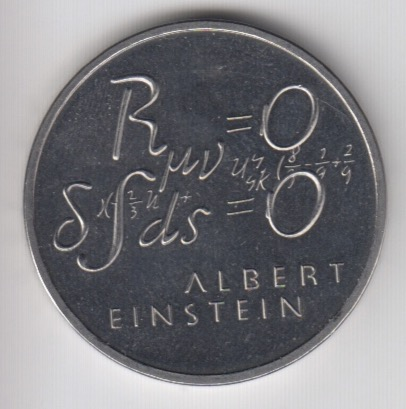
\includegraphics[width=5cm]{papers/Einstein5Fr.jpg}
\caption{Variationsprinzip der Relativitätstheorie auf dem
Gedenkfünfliber zum 100.~Geburtstag von Albert Einstein
aus dem Jahr 1979.
Die Bewegungsgleichungen der Relativitätstheorie lassen sich aus
dem Variationsproblen $\delta \int ds=0$ ableiten.
\label{buch:papers:fig:5liber}}
\end{figure}%
Auch in der relativistische Mechanik lassen sich die Bewegungsgleichungen
aus einem Variationsprinzip ableiten, welches man sogar auf
dem Gedenkfünfliber zum 100.~Geburtstag Albert Einsteins aus dem
Jahr 1975 finden kann (Abbildung~\ref{buch:papers:fig:5liber}).
\textit{Selvin Blöchlinger} leitet die relativistischen
Bewegungsgleichungen für ein geladenes Teilchen in einem
elektromagnetischen Feld ab.

Die Gleichungen des elektromagnetischen Feldes werden normalerweise
durch die Maxwell-Gleichungen beschrieben.
\textit{Maurin Doswald}
und
\textit{Stephan Oseghale}
leiten sie aus einem Variationsprinzip her.

Das Variationsprinzip, welches die relativistischen Bewegungsgleichungen
liefern, ist eigentlich ein Minimalproblem für die Kurvenlänge.
Solche Kurven heissen Geodäten.
\textit{Andrin Kälin}
und
\textit{Marco Rouge}
entwickeln den Formalismus der Geodätendifferentialgleichung aus
den Euler-Lagrange-Differentialgleichungen für die Kurvenlänge.

Auch für die Gleichungen, die das Verhalten elektrischer Ströme in 
einer Schaltung beschreiben, lässt sich ein Variationsprinzip 
finden.
Es ermöglicht, die Stromverteilung auch in kontinuierlich verteilten
Medien zu berechnen, wie dies \textit{Matthias Meyer} durchführt.

An der Schnittstelle zwischen einer Schaltung und dem elektromagnetischen
Feld steht jeweils eine Antenne.
\textit{Baris Catan}
und
\textit{Jannis Gull}
zeigen, wie man die Form einer Antenne mit dem Ritz-Verfahren,
einem direkten Verfahren der Variationsrechnung,
optimieren kann.

Schon Leonhard Euler hat sich mit der Frage befasst, wie man 
am schnellsten durch die Strömung eines Flusses schwimmt.
\textit{Anna Pietak} untersucht dieser Frage in Ihrer Arbeit.

Allgemeiner einsetzbar als das Ritz-Verfahren ist die Methode
der finiten Elemente, in die \textit{Flurin Brechbühler} einführt.

Ein besonders anspruchsvolles Minimalproblem ist die Aufgabe,
eine Nutzlast mit Hilfe einer Rakete in eine Erdumlaufbahn zu
bringen.
\textit{Joel Stohler}
und
\textit{David Peter}
zeigen, dass diese Aufgabe auf ein optimales Steuerungsproblem
führt.

Warum sind alle Planeten kugelförmig?
\textit{Jakob Gierer}
und 
\textit{Lukas Schöpf}
lösen das Problem des hydrostatischen Gleichgewichts und
zeigen so, dass die Form geringster Energie eine Kugel ist.

Der Begriff Variation wird auch für Algorithmen verwendet.
\textit{Kevin Kempf} führt in dieses Thema ein und stellt
einen Vergleich zur Variationsrechnung an.

Die Entmischung von Legierungen wird durch die Cahn-Hilliard-Gleichung
beschrieben.
\textit{Patrik Müller} stellt den unmittelbaren Praxisbezug her,
indem er nicht nur die Gleichung herleitet, sondern auch auf
das Problem anwendet, eine gute Salatsauce herzustellen.








% einzelne Artikel 
\label{buch:part2:anwendungen}
%
% addpapers.tex -- file to add all paper main files
%
% (c) 2023 Prof Dr Andreas Müller, OST Ostschweizer Fachhochschule
%
%
% main.tex -- Paper zum Thema <relativ>
%
% (c) 2020 Autor, OST Ostschweizer Fachhochschule
%
% !TEX root = ../../buch.tex
% !TEX encoding = UTF-8
%
% git checkout dev -- sections images main.tex packages.tex references.bib Makefile Makefile.inc .gitignore
%

\chapter{Relativistische Mechanik\label{chapter:relativ}}
\kopflinks{Thema}
\begin{refsection}
\chapterauthor{Selvin Blöchlinger}

Das vorliegende Kapitel behandelt die Herleitung der Gesetze der relativistischen Mechanik
mithilfe der Variationsrechnung.
Es stützt sich grösstenteils auf~\cite{relativ:landau}.

\input{papers/relativ/sections/relativistik.tex}
\input{papers/relativ/sections/rel_mechanik.tex}
\input{papers/relativ/sections/em_feld.tex}


\printbibliography[heading=subbibliography]
\end{refsection}

%
% main.tex -- Paper zum Thema <relativ>
%
% (c) 2020 Autor, OST Ostschweizer Fachhochschule
%
% !TEX root = ../../buch.tex
% !TEX encoding = UTF-8
%
% git checkout dev -- sections images main.tex packages.tex references.bib Makefile Makefile.inc .gitignore
%

\chapter{Relativistische Mechanik\label{chapter:relativ}}
\kopflinks{Thema}
\begin{refsection}
\chapterauthor{Selvin Blöchlinger}

Das vorliegende Kapitel behandelt die Herleitung der Gesetze der relativistischen Mechanik
mithilfe der Variationsrechnung.
Es stützt sich grösstenteils auf~\cite{relativ:landau}.

\input{papers/relativ/sections/relativistik.tex}
\input{papers/relativ/sections/rel_mechanik.tex}
\input{papers/relativ/sections/em_feld.tex}


\printbibliography[heading=subbibliography]
\end{refsection}

%
% main.tex -- Paper zum Thema <relativ>
%
% (c) 2020 Autor, OST Ostschweizer Fachhochschule
%
% !TEX root = ../../buch.tex
% !TEX encoding = UTF-8
%
% git checkout dev -- sections images main.tex packages.tex references.bib Makefile Makefile.inc .gitignore
%

\chapter{Relativistische Mechanik\label{chapter:relativ}}
\kopflinks{Thema}
\begin{refsection}
\chapterauthor{Selvin Blöchlinger}

Das vorliegende Kapitel behandelt die Herleitung der Gesetze der relativistischen Mechanik
mithilfe der Variationsrechnung.
Es stützt sich grösstenteils auf~\cite{relativ:landau}.

\input{papers/relativ/sections/relativistik.tex}
\input{papers/relativ/sections/rel_mechanik.tex}
\input{papers/relativ/sections/em_feld.tex}


\printbibliography[heading=subbibliography]
\end{refsection}

%
% main.tex -- Paper zum Thema <relativ>
%
% (c) 2020 Autor, OST Ostschweizer Fachhochschule
%
% !TEX root = ../../buch.tex
% !TEX encoding = UTF-8
%
% git checkout dev -- sections images main.tex packages.tex references.bib Makefile Makefile.inc .gitignore
%

\chapter{Relativistische Mechanik\label{chapter:relativ}}
\kopflinks{Thema}
\begin{refsection}
\chapterauthor{Selvin Blöchlinger}

Das vorliegende Kapitel behandelt die Herleitung der Gesetze der relativistischen Mechanik
mithilfe der Variationsrechnung.
Es stützt sich grösstenteils auf~\cite{relativ:landau}.

\input{papers/relativ/sections/relativistik.tex}
\input{papers/relativ/sections/rel_mechanik.tex}
\input{papers/relativ/sections/em_feld.tex}


\printbibliography[heading=subbibliography]
\end{refsection}

%
% main.tex -- Paper zum Thema <relativ>
%
% (c) 2020 Autor, OST Ostschweizer Fachhochschule
%
% !TEX root = ../../buch.tex
% !TEX encoding = UTF-8
%
% git checkout dev -- sections images main.tex packages.tex references.bib Makefile Makefile.inc .gitignore
%

\chapter{Relativistische Mechanik\label{chapter:relativ}}
\kopflinks{Thema}
\begin{refsection}
\chapterauthor{Selvin Blöchlinger}

Das vorliegende Kapitel behandelt die Herleitung der Gesetze der relativistischen Mechanik
mithilfe der Variationsrechnung.
Es stützt sich grösstenteils auf~\cite{relativ:landau}.

\input{papers/relativ/sections/relativistik.tex}
\input{papers/relativ/sections/rel_mechanik.tex}
\input{papers/relativ/sections/em_feld.tex}


\printbibliography[heading=subbibliography]
\end{refsection}

%
% main.tex -- Paper zum Thema <relativ>
%
% (c) 2020 Autor, OST Ostschweizer Fachhochschule
%
% !TEX root = ../../buch.tex
% !TEX encoding = UTF-8
%
% git checkout dev -- sections images main.tex packages.tex references.bib Makefile Makefile.inc .gitignore
%

\chapter{Relativistische Mechanik\label{chapter:relativ}}
\kopflinks{Thema}
\begin{refsection}
\chapterauthor{Selvin Blöchlinger}

Das vorliegende Kapitel behandelt die Herleitung der Gesetze der relativistischen Mechanik
mithilfe der Variationsrechnung.
Es stützt sich grösstenteils auf~\cite{relativ:landau}.

\input{papers/relativ/sections/relativistik.tex}
\input{papers/relativ/sections/rel_mechanik.tex}
\input{papers/relativ/sections/em_feld.tex}


\printbibliography[heading=subbibliography]
\end{refsection}

%
% main.tex -- Paper zum Thema <relativ>
%
% (c) 2020 Autor, OST Ostschweizer Fachhochschule
%
% !TEX root = ../../buch.tex
% !TEX encoding = UTF-8
%
% git checkout dev -- sections images main.tex packages.tex references.bib Makefile Makefile.inc .gitignore
%

\chapter{Relativistische Mechanik\label{chapter:relativ}}
\kopflinks{Thema}
\begin{refsection}
\chapterauthor{Selvin Blöchlinger}

Das vorliegende Kapitel behandelt die Herleitung der Gesetze der relativistischen Mechanik
mithilfe der Variationsrechnung.
Es stützt sich grösstenteils auf~\cite{relativ:landau}.

\input{papers/relativ/sections/relativistik.tex}
\input{papers/relativ/sections/rel_mechanik.tex}
\input{papers/relativ/sections/em_feld.tex}


\printbibliography[heading=subbibliography]
\end{refsection}

%
% main.tex -- Paper zum Thema <relativ>
%
% (c) 2020 Autor, OST Ostschweizer Fachhochschule
%
% !TEX root = ../../buch.tex
% !TEX encoding = UTF-8
%
% git checkout dev -- sections images main.tex packages.tex references.bib Makefile Makefile.inc .gitignore
%

\chapter{Relativistische Mechanik\label{chapter:relativ}}
\kopflinks{Thema}
\begin{refsection}
\chapterauthor{Selvin Blöchlinger}

Das vorliegende Kapitel behandelt die Herleitung der Gesetze der relativistischen Mechanik
mithilfe der Variationsrechnung.
Es stützt sich grösstenteils auf~\cite{relativ:landau}.

\input{papers/relativ/sections/relativistik.tex}
\input{papers/relativ/sections/rel_mechanik.tex}
\input{papers/relativ/sections/em_feld.tex}


\printbibliography[heading=subbibliography]
\end{refsection}

%
% main.tex -- Paper zum Thema <relativ>
%
% (c) 2020 Autor, OST Ostschweizer Fachhochschule
%
% !TEX root = ../../buch.tex
% !TEX encoding = UTF-8
%
% git checkout dev -- sections images main.tex packages.tex references.bib Makefile Makefile.inc .gitignore
%

\chapter{Relativistische Mechanik\label{chapter:relativ}}
\kopflinks{Thema}
\begin{refsection}
\chapterauthor{Selvin Blöchlinger}

Das vorliegende Kapitel behandelt die Herleitung der Gesetze der relativistischen Mechanik
mithilfe der Variationsrechnung.
Es stützt sich grösstenteils auf~\cite{relativ:landau}.

\input{papers/relativ/sections/relativistik.tex}
\input{papers/relativ/sections/rel_mechanik.tex}
\input{papers/relativ/sections/em_feld.tex}


\printbibliography[heading=subbibliography]
\end{refsection}

%
% main.tex -- Paper zum Thema <relativ>
%
% (c) 2020 Autor, OST Ostschweizer Fachhochschule
%
% !TEX root = ../../buch.tex
% !TEX encoding = UTF-8
%
% git checkout dev -- sections images main.tex packages.tex references.bib Makefile Makefile.inc .gitignore
%

\chapter{Relativistische Mechanik\label{chapter:relativ}}
\kopflinks{Thema}
\begin{refsection}
\chapterauthor{Selvin Blöchlinger}

Das vorliegende Kapitel behandelt die Herleitung der Gesetze der relativistischen Mechanik
mithilfe der Variationsrechnung.
Es stützt sich grösstenteils auf~\cite{relativ:landau}.

\input{papers/relativ/sections/relativistik.tex}
\input{papers/relativ/sections/rel_mechanik.tex}
\input{papers/relativ/sections/em_feld.tex}


\printbibliography[heading=subbibliography]
\end{refsection}

%
% main.tex -- Paper zum Thema <relativ>
%
% (c) 2020 Autor, OST Ostschweizer Fachhochschule
%
% !TEX root = ../../buch.tex
% !TEX encoding = UTF-8
%
% git checkout dev -- sections images main.tex packages.tex references.bib Makefile Makefile.inc .gitignore
%

\chapter{Relativistische Mechanik\label{chapter:relativ}}
\kopflinks{Thema}
\begin{refsection}
\chapterauthor{Selvin Blöchlinger}

Das vorliegende Kapitel behandelt die Herleitung der Gesetze der relativistischen Mechanik
mithilfe der Variationsrechnung.
Es stützt sich grösstenteils auf~\cite{relativ:landau}.

\input{papers/relativ/sections/relativistik.tex}
\input{papers/relativ/sections/rel_mechanik.tex}
\input{papers/relativ/sections/em_feld.tex}


\printbibliography[heading=subbibliography]
\end{refsection}

%
% main.tex -- Paper zum Thema <relativ>
%
% (c) 2020 Autor, OST Ostschweizer Fachhochschule
%
% !TEX root = ../../buch.tex
% !TEX encoding = UTF-8
%
% git checkout dev -- sections images main.tex packages.tex references.bib Makefile Makefile.inc .gitignore
%

\chapter{Relativistische Mechanik\label{chapter:relativ}}
\kopflinks{Thema}
\begin{refsection}
\chapterauthor{Selvin Blöchlinger}

Das vorliegende Kapitel behandelt die Herleitung der Gesetze der relativistischen Mechanik
mithilfe der Variationsrechnung.
Es stützt sich grösstenteils auf~\cite{relativ:landau}.

\input{papers/relativ/sections/relativistik.tex}
\input{papers/relativ/sections/rel_mechanik.tex}
\input{papers/relativ/sections/em_feld.tex}


\printbibliography[heading=subbibliography]
\end{refsection}

%
% main.tex -- Paper zum Thema <relativ>
%
% (c) 2020 Autor, OST Ostschweizer Fachhochschule
%
% !TEX root = ../../buch.tex
% !TEX encoding = UTF-8
%
% git checkout dev -- sections images main.tex packages.tex references.bib Makefile Makefile.inc .gitignore
%

\chapter{Relativistische Mechanik\label{chapter:relativ}}
\kopflinks{Thema}
\begin{refsection}
\chapterauthor{Selvin Blöchlinger}

Das vorliegende Kapitel behandelt die Herleitung der Gesetze der relativistischen Mechanik
mithilfe der Variationsrechnung.
Es stützt sich grösstenteils auf~\cite{relativ:landau}.

\input{papers/relativ/sections/relativistik.tex}
\input{papers/relativ/sections/rel_mechanik.tex}
\input{papers/relativ/sections/em_feld.tex}


\printbibliography[heading=subbibliography]
\end{refsection}

%
% main.tex -- Paper zum Thema <relativ>
%
% (c) 2020 Autor, OST Ostschweizer Fachhochschule
%
% !TEX root = ../../buch.tex
% !TEX encoding = UTF-8
%
% git checkout dev -- sections images main.tex packages.tex references.bib Makefile Makefile.inc .gitignore
%

\chapter{Relativistische Mechanik\label{chapter:relativ}}
\kopflinks{Thema}
\begin{refsection}
\chapterauthor{Selvin Blöchlinger}

Das vorliegende Kapitel behandelt die Herleitung der Gesetze der relativistischen Mechanik
mithilfe der Variationsrechnung.
Es stützt sich grösstenteils auf~\cite{relativ:landau}.

\input{papers/relativ/sections/relativistik.tex}
\input{papers/relativ/sections/rel_mechanik.tex}
\input{papers/relativ/sections/em_feld.tex}


\printbibliography[heading=subbibliography]
\end{refsection}

%
% main.tex -- Paper zum Thema <relativ>
%
% (c) 2020 Autor, OST Ostschweizer Fachhochschule
%
% !TEX root = ../../buch.tex
% !TEX encoding = UTF-8
%
% git checkout dev -- sections images main.tex packages.tex references.bib Makefile Makefile.inc .gitignore
%

\chapter{Relativistische Mechanik\label{chapter:relativ}}
\kopflinks{Thema}
\begin{refsection}
\chapterauthor{Selvin Blöchlinger}

Das vorliegende Kapitel behandelt die Herleitung der Gesetze der relativistischen Mechanik
mithilfe der Variationsrechnung.
Es stützt sich grösstenteils auf~\cite{relativ:landau}.

\input{papers/relativ/sections/relativistik.tex}
\input{papers/relativ/sections/rel_mechanik.tex}
\input{papers/relativ/sections/em_feld.tex}


\printbibliography[heading=subbibliography]
\end{refsection}

%
% main.tex -- Paper zum Thema <relativ>
%
% (c) 2020 Autor, OST Ostschweizer Fachhochschule
%
% !TEX root = ../../buch.tex
% !TEX encoding = UTF-8
%
% git checkout dev -- sections images main.tex packages.tex references.bib Makefile Makefile.inc .gitignore
%

\chapter{Relativistische Mechanik\label{chapter:relativ}}
\kopflinks{Thema}
\begin{refsection}
\chapterauthor{Selvin Blöchlinger}

Das vorliegende Kapitel behandelt die Herleitung der Gesetze der relativistischen Mechanik
mithilfe der Variationsrechnung.
Es stützt sich grösstenteils auf~\cite{relativ:landau}.

\input{papers/relativ/sections/relativistik.tex}
\input{papers/relativ/sections/rel_mechanik.tex}
\input{papers/relativ/sections/em_feld.tex}


\printbibliography[heading=subbibliography]
\end{refsection}

%
% main.tex -- Paper zum Thema <relativ>
%
% (c) 2020 Autor, OST Ostschweizer Fachhochschule
%
% !TEX root = ../../buch.tex
% !TEX encoding = UTF-8
%
% git checkout dev -- sections images main.tex packages.tex references.bib Makefile Makefile.inc .gitignore
%

\chapter{Relativistische Mechanik\label{chapter:relativ}}
\kopflinks{Thema}
\begin{refsection}
\chapterauthor{Selvin Blöchlinger}

Das vorliegende Kapitel behandelt die Herleitung der Gesetze der relativistischen Mechanik
mithilfe der Variationsrechnung.
Es stützt sich grösstenteils auf~\cite{relativ:landau}.

\input{papers/relativ/sections/relativistik.tex}
\input{papers/relativ/sections/rel_mechanik.tex}
\input{papers/relativ/sections/em_feld.tex}


\printbibliography[heading=subbibliography]
\end{refsection}

%
% main.tex -- Paper zum Thema <relativ>
%
% (c) 2020 Autor, OST Ostschweizer Fachhochschule
%
% !TEX root = ../../buch.tex
% !TEX encoding = UTF-8
%
% git checkout dev -- sections images main.tex packages.tex references.bib Makefile Makefile.inc .gitignore
%

\chapter{Relativistische Mechanik\label{chapter:relativ}}
\kopflinks{Thema}
\begin{refsection}
\chapterauthor{Selvin Blöchlinger}

Das vorliegende Kapitel behandelt die Herleitung der Gesetze der relativistischen Mechanik
mithilfe der Variationsrechnung.
Es stützt sich grösstenteils auf~\cite{relativ:landau}.

\input{papers/relativ/sections/relativistik.tex}
\input{papers/relativ/sections/rel_mechanik.tex}
\input{papers/relativ/sections/em_feld.tex}


\printbibliography[heading=subbibliography]
\end{refsection}





\vfill
\pagebreak
\ifodd\value{page}\else\null\clearpage\fi
\fancyhead[RE]{Index}
\fancyhead[LO]{Index}
\addcontentsline{toc}{chapter}{\indexname}
\ifthenelse{\boolean{includecover}}{
\InputIfFileExists{build/SeminarVariation.ind}{}{}
}{
\InputIfFileExists{build/buch.ind}{}{}
}

% cover page
\ifthenelse{\boolean{includecover}}{
%\newpage\null%
\thispagestyle{empty}%
\newpage%
\incgraph[documentpaper][width=\paperwidth,height=\paperheight]{../cover/back2.jpg}
}{}%
\end{document}
